\documentclass[twoside]{article}

% Packages required by doxygen
\usepackage{calc}
\usepackage{doxygen}
\usepackage{graphicx}
\usepackage[utf8]{inputenc}
\usepackage{makeidx}
\usepackage{multicol}
\usepackage{multirow}
\usepackage{textcomp}
\usepackage[table]{xcolor}

% Font selection
\usepackage[T1]{fontenc}
\usepackage{mathptmx}
\usepackage[scaled=.90]{helvet}
\usepackage{courier}
\usepackage{amssymb}
\usepackage{sectsty}
\renewcommand{\familydefault}{\sfdefault}
\allsectionsfont{%
  \fontseries{bc}\selectfont%
  \color{darkgray}%
}
\renewcommand{\DoxyLabelFont}{%
  \fontseries{bc}\selectfont%
  \color{darkgray}%
}

% Page & text layout
\usepackage{geometry}
\geometry{%
  a4paper,%
  top=2.5cm,%
  bottom=2.5cm,%
  left=2.5cm,%
  right=2.5cm%
}
\tolerance=750
\hfuzz=15pt
\hbadness=750
\setlength{\emergencystretch}{15pt}
\setlength{\parindent}{0cm}
\setlength{\parskip}{0.2cm}
\makeatletter
\renewcommand{\paragraph}{%
  \@startsection{paragraph}{4}{0ex}{-1.0ex}{1.0ex}{%
    \normalfont\normalsize\bfseries\SS@parafont%
  }%
}
\renewcommand{\subparagraph}{%
  \@startsection{subparagraph}{5}{0ex}{-1.0ex}{1.0ex}{%
    \normalfont\normalsize\bfseries\SS@subparafont%
  }%
}
\makeatother

% Headers & footers
\usepackage{fancyhdr}
\pagestyle{fancyplain}
\fancyhead[LE]{\fancyplain{}{\bfseries\thepage}}
\fancyhead[CE]{\fancyplain{}{}}
\fancyhead[RE]{\fancyplain{}{\bfseries\leftmark}}
\fancyhead[LO]{\fancyplain{}{\bfseries\rightmark}}
\fancyhead[CO]{\fancyplain{}{}}
\fancyhead[RO]{\fancyplain{}{\bfseries\thepage}}
\fancyfoot[LE]{\fancyplain{}{}}
\fancyfoot[CE]{\fancyplain{}{}}
\fancyfoot[RE]{\fancyplain{}{\bfseries\scriptsize Generated on Sat Nov 30 2013 20\-:21\-:20 for e\-Solid -\/ Real-\/\-Time Kernel by Doxygen }}
\fancyfoot[LO]{\fancyplain{}{\bfseries\scriptsize Generated on Sat Nov 30 2013 20\-:21\-:20 for e\-Solid -\/ Real-\/\-Time Kernel by Doxygen }}
\fancyfoot[CO]{\fancyplain{}{}}
\fancyfoot[RO]{\fancyplain{}{}}
\renewcommand{\footrulewidth}{0.4pt}
\renewcommand{\sectionmark}[1]{%
  \markright{\thesection\ #1}%
}

% Indices & bibliography
\usepackage{natbib}
\usepackage[titles]{tocloft}
\setcounter{tocdepth}{3}
\setcounter{secnumdepth}{5}
\makeindex

% Hyperlinks (required, but should be loaded last)
\usepackage{ifpdf}
\ifpdf
  \usepackage[pdftex,pagebackref=true]{hyperref}
\else
  \usepackage[ps2pdf,pagebackref=true]{hyperref}
\fi
\hypersetup{%
  colorlinks=true,%
  linkcolor=blue,%
  citecolor=blue,%
  unicode%
}

% Custom commands
\newcommand{\clearemptydoublepage}{%
  \newpage{\pagestyle{empty}\cleardoublepage}%
}


%===== C O N T E N T S =====

\begin{document}

% Titlepage & ToC
\hypersetup{pageanchor=false}
\pagenumbering{roman}
\begin{titlepage}
\vspace*{7cm}
\begin{center}%
{\Large e\-Solid -\/ Real-\/\-Time Kernel \\[1ex]\large 1.\-0\-Beta\-R02 }\\
\vspace*{1cm}
{\large Generated by Doxygen 1.8.5}\\
\vspace*{0.5cm}
{\small Sat Nov 30 2013 20:21:20}\\
\end{center}
\end{titlepage}
\tableofcontents
\pagenumbering{arabic}
\hypersetup{pageanchor=true}

%--- Begin generated contents ---
\section{Overview}
\label{index}\hypertarget{index}{}\hypertarget{index_kernel_specs}{}\subsection{e\-Solid -\/ R\-T Kernel Features}\label{index_kernel_specs}
\hypertarget{index_spec_source}{}\subsubsection{Source code}\label{index_spec_source}
The source code of the kernel and all of it's ports are published under {\bfseries free software license}, which guarantees end users (individuals, organizations, companies) the freedoms to use, study, share (copy), and modify the software.

The G\-P\-L grants the recipients of a computer software the rights of the Free Software Definition (written by Richard Stallman) and uses copyleft to ensure the freedoms are preserved whenever the work is distributed, even when the work is changed or added to. The G\-P\-L is a copyleft license, which means that derived works can only be distributed under the same license terms.

For more details visit\-: \href{https://gnu.org/licenses/gpl.html}{\tt https\-://gnu.\-org/licenses/gpl.\-html}\hypertarget{index_spec_api}{}\subsubsection{Consistent Application Programming Interface}\label{index_spec_api}
\begin{DoxyParagraph}{Coding style}
All public objects declared in Application Programming Interface are following this coding style\-:
\begin{DoxyItemize}
\item All objects except macros are using {\ttfamily camel\-Case} style names
\item All functions, structures and unions are prefixed with\-: {\ttfamily es}
\item All typedef-\/ed types are prefixed with\-: {\ttfamily es} and postfixed with\-: {\ttfamily \-\_\-\-T}
\item All macro names are in {\ttfamily U\-P\-P\-E\-R\-C\-A\-S\-E} style, words are delimited by underscore sign
\item All macro names are prefixed with\-: {\ttfamily E\-S\-\_\-}
\item The first letter of global variables is in upper case.
\end{DoxyItemize}
\end{DoxyParagraph}
\begin{DoxyParagraph}{A\-P\-I object naming rules}
All A\-P\-I objects are named following this convention\-: {\ttfamily $<$group$>$$<$action$>$$<$suffix$>$}
\end{DoxyParagraph}

\begin{DoxyItemize}
\item Group\-:
\begin{DoxyItemize}
\item {\ttfamily Kern} -\/ General Kernel services
\item {\ttfamily Thd} -\/ Thread management
\item {\ttfamily Thd\-Q} -\/ Thread Queue management
\item {\ttfamily Sched} -\/ Scheduler invocation and Scheduler Ready Queue management
\item {\ttfamily V\-Tmr} -\/ Virtual Timer management
\item {\ttfamily user} -\/ Application callback functions
\end{DoxyItemize}
\item Suffix\-:
\begin{DoxyItemize}
\item {\ttfamily none} -\/ normal A\-P\-I object
\item {\ttfamily I} -\/ I class -\/ Regular Interrupts are locked
\end{DoxyItemize}
\end{DoxyItemize}

All Port Interface objects are named using the rules stated above with certain differences\-:
\begin{DoxyItemize}
\item All functions, structures and unions are prefixed with\-: {\ttfamily port}
\item All macro names are prefixed with\-: {\ttfamily P\-O\-R\-T\-\_\-}
\item Port specific objects are prefixed with {\ttfamily C\-P\-U\-\_\-} or {\ttfamily cpu}.
\end{DoxyItemize}\hypertarget{index_spec_preempt}{}\subsubsection{Preemptive multi-\/threading}\label{index_spec_preempt}
e\-Solid -\/ R\-T Kernel uses a {\bfseries preemptive scheduler}, which has the power to preempt, or interrupt, and later resume, other threads in the system. The scheduler always runs ready thread with the highest priority.\hypertarget{index_spec_rr}{}\subsubsection{Round-\/\-Robin scheduling}\label{index_spec_rr}
Round-\/\-Robin scheduling is very {\bfseries simple algorithm} to implement and it is starvation free$\ast$$\ast$. It employs time-\/sharing, giving to each thread a time slice or {\ttfamily quantum}. Processor's time is shared between a number of threads, giving the illusion that it is dealing with these threads {\bfseries concurrently}. This scheduling is only used when there are two or more threads of the same priority ready for execution.\hypertarget{index_spec_deterministic}{}\subsubsection{Deterministic}\label{index_spec_deterministic}
Majority of algorithms used in e\-Solid -\/ R\-T Kernel implementation are belonging to Constant Time Complexity$\ast$$\ast$ category. Constant Time {\ttfamily O(1)} functions needs fixed amount of time to execute an algorithm. In other words the execution time of Constant Time Complexity functions does not depend on number of inputs. For more information see \hyperlink{time_complexity}{Time complexity}.\hypertarget{index_spec_cfg}{}\subsubsection{Configurable}\label{index_spec_cfg}
The kernel provides two configuration files \hyperlink{kernel__cfg_8h}{kernel\-\_\-cfg.\-h} and cpu\-\_\-cfg.\-h which can be used to tailor the kernel to application needs.

In addition, the kernel implements a number of hooks which can alter or augment the behavior of the kernel or applications, by intercepting function calls between software components.\hypertarget{index_spec_portable}{}\subsubsection{Portable}\label{index_spec_portable}
During the design stage of the kernel a special attention was given to achieve high portability of the kernel. Some data structures and algorithms are tailored to exploit new hardware features.\hypertarget{index_spec_static}{}\subsubsection{Static object allocation}\label{index_spec_static}
All objects used in e\-Solid -\/ R\-T Kernel can be statically allocated. There is no need to use any memory management functionality which makes it very easy to verify the application.\hypertarget{index_spec_unlimited}{}\subsubsection{Unlimited number of threads}\label{index_spec_unlimited}
e\-Solid -\/ R\-T Kernel allows applications to have any number of threads. The only limiting factors for the maximum number of threads are the amount of R\-A\-M and R\-O\-M memory capacity and required processing time.\hypertarget{index_spec_prio}{}\subsubsection{Up to 256 thread priority levels}\label{index_spec_prio}
Each thread has a defined priority. Lowest priority level is 0, while the highest available level is configurable. If Round-\/\-Robin scheduling is used then multiple threads can be in the same priority level. If Round-\/\-Robin scheduling is disabled then each thread must have unique priority level. The priority sorting algorithm has constant time complexity which means it always executes in the same time period regardles of the levels of priority used.\hypertarget{index_spec_tickless}{}\subsubsection{Tickless idle}\label{index_spec_tickless}
Classic kernel architectures periodically interrupted C\-P\-U at a predetermined frequency — 100 Hz, 250 Hz, or 1000 Hz, depending on the application needs. Known as the system timer tick, the kernel performed this interrupt regardless of the power state of the C\-P\-U. Therefore, even an idle C\-P\-U was responding to up to 1000 of these requests every second. On systems that implemented power saving measures for idle C\-P\-Us, the timer tick prevented the C\-P\-U from remaining idle long enough for the system to benefit from these power savings.

The e\-Solid R\-T kernel runs in tickless idle\-: that is, it replaces the old periodic timer interrupts with on-\/demand interrupts. Therefore, idle C\-P\-Us are allowed to remain idle until a new task is queued for processing, and C\-P\-Us that have entered lower power states can remain in these states longer.\hypertarget{index_spec_errchk}{}\subsubsection{Error checking}\label{index_spec_errchk}
All e\-Solid software is using design methods very similar to approaches of contract programming$\ast$$\ast$ paradigm for software design. The contract programming prescribes that Application Programming Interface should have formal, precise and verifiable specifications, which extend the ordinary definition of abstract data types with preconditions and postconditions. These specifications are referred to as \char`\"{}contracts\char`\"{}. The contract for each method will normally contain the following pieces of information\-:


\begin{DoxyItemize}
\item Acceptable and unacceptable input values
\item Return values and their meanings
\item Error and exception condition values that can occur during the execution
\item Side effects
\item Preconditions
\item Postconditions
\item Invariants
\end{DoxyItemize}

The contract validations are done by {\bfseries assert} macros. They have the responsibility of informing the programmer when a contract can not be validated.\hypertarget{index_spec_prof}{}\subsubsection{Profiling}\label{index_spec_prof}
\begin{DoxyNote}{Note}
This feature is not implemented 
\end{DoxyNote}

\section{Directory and file organization}
\label{files_org}
\hypertarget{files_org}{}
Details about directory and file organization\hypertarget{files_org_files_intro}{}\subsection{Intro}\label{files_org_files_intro}
The directory structure of e\-Solid -\/ R\-T Kernel is should be easy to understand. Once the organization of directories and files is understood it is fairly easy to integrate e\-Solid -\/ R\-T Kernel into application project.\hypertarget{files_org_files_porting}{}\subsubsection{What is a port?}\label{files_org_files_porting}
Porting is a process of adapting software to an architecture that is different from the one for which it was originally designed. The term is also used when software is changed to make it usable in different environments. Software is portable when the cost of porting it to a new platform is less than the cost of writing it from beginning.\hypertarget{files_org_files_sections}{}\subsection{Code Sections}\label{files_org_files_sections}
The kernel is divided into three sections. One section is port independent code, the second one is port dependent code and the third sections is code templates.\hypertarget{files_org_files_icode}{}\subsubsection{Port independent code}\label{files_org_files_icode}
Port independent code is the code which does not change from port to port, e.\-g. when the C\-P\-U is changed this code is not changed at all and it is still correctly executed. Code can be developed and tested on another machine, which greatly reduces design efforts. It provides A\-P\-I and some common data structures. Port independent code lives under {\ttfamily /inc} and {\ttfamily /src} directories\-:
\begin{DoxyItemize}
\item {\ttfamily \hyperlink{kernel_8h}{inc/kernel/kernel.\-h}}
\item {\ttfamily inc/kernel/kernel\-\_\-cfg.\-h} (application specific -\/ see template)
\item {\ttfamily \hyperlink{kernel_8c}{src/kernel.\-c}}
\item {\ttfamily inc/kernel/dbg.\-h}
\item {\ttfamily inc/kernel/dbg\-\_\-cfg.\-h} (application specific -\/ see template)
\item {\ttfamily src/dbg.\-c}
\end{DoxyItemize}

Click on file name for further description of the file.\hypertarget{files_org_files_dcode}{}\subsubsection{Port dependent code}\label{files_org_files_dcode}
Second section is the port dependent code. This code provides low-\/level functions which are needed to interact with interrupt controllers, manipulate C\-P\-U settings and do the context switching. They are highly C\-P\-U/compiler bounded and are often written in assembly language.

Each port has it's name which is also the name of directory which holds all the port files. Usually each port has some kind of variant/architecture. In that case each variant is a subdirectory of the containing port. Common code for all variants will be in common subdirectory. Each e\-Solid -\/ R\-T Kernel port will have at least the following files\-:
\begin{DoxyItemize}
\item {\ttfamily port/\mbox{[}port\-\_\-name\mbox{]}/common/arch/compiler.h}
\item {\ttfamily port/\mbox{[}port\-\_\-name\mbox{]}/\mbox{[}architecture\-\_\-name\mbox{]}/arch/cpu\-\_\-cfg.h}
\item {\ttfamily port/\mbox{[}port\-\_\-name\mbox{]}/\mbox{[}architecture\-\_\-name\mbox{]}/arch/cpu.h}
\item {\ttfamily port/\mbox{[}port\-\_\-name\mbox{]}/\mbox{[}architecture\-\_\-name\mbox{]}/cpu.c}
\item {\ttfamily port/\mbox{[}port\-\_\-name\mbox{]}/\mbox{[}family\-\_\-name\mbox{]}/family/profile.h}
\end{DoxyItemize}

\begin{DoxyNote}{Note}
Port dependent code is separately described in documentation for relevant port. 
\end{DoxyNote}
\hypertarget{files_org_files_template}{}\subsubsection{Template and example code}\label{files_org_files_template}
Templates are some predefined configuration settings for various scenarios where e\-Solid -\/ R\-T Kernel can be used. Templates also contain some example code for how to write new ports.

In the example below is given {\ttfamily Generic} template which holds files with default configuration settings and some example code for new ports. New port files are in template/generic/port directory. When porting to a new architecture/compiler use provided template files for starters. This will greatly reduce the time needed to become familiar with the kernel port requirements. Generic template files are the following\-:
\begin{DoxyItemize}
\item {\ttfamily \hyperlink{compiler_8h}{template/generic/\-\_\-port\-\_\-/common/arch/compiler.\-h}}
\item {\ttfamily template/generic/\-\_\-port\-\_\-/\-\_\-cpu\-\_\-/arch/cpu\-\_\-cfg.\-h}
\item {\ttfamily template/generic/\-\_\-port\-\_\-/\-\_\-cpu\-\_\-/arch/cpu.\-h}
\item {\ttfamily template/generic/\-\_\-port\-\_\-/\-\_\-cpu\-\_\-/cpu.\-c}
\item {\ttfamily \hyperlink{profile_8h}{template/generic/\-\_\-port\-\_\-/\-\_\-mcu\-\_\-/family/profile.\-h}}
\item {\ttfamily \hyperlink{kernel__cfg_8h}{template/generic/kernel\-\_\-cfg.\-h}}
\item {\ttfamily template/generic/dbg\-\_\-cfg.\-h} 
\end{DoxyItemize}
\section{Kernel states}
\label{states}
\hypertarget{states}{}
Details about kernel states

\par
\par
\par
\hypertarget{states_states_intro}{}\subsection{Intro}\label{states_states_intro}
A Kernel state machine is a behavior model of the kernel core. Each state defines what methods are allowed.\hypertarget{states_states_fsm}{}\subsection{e\-Solid R\-T Kernel states}\label{states_states_fsm}
The kernel can be in one of the following states\-: \begin{center}

\begin{DoxyImageNoCaption}
  \mbox{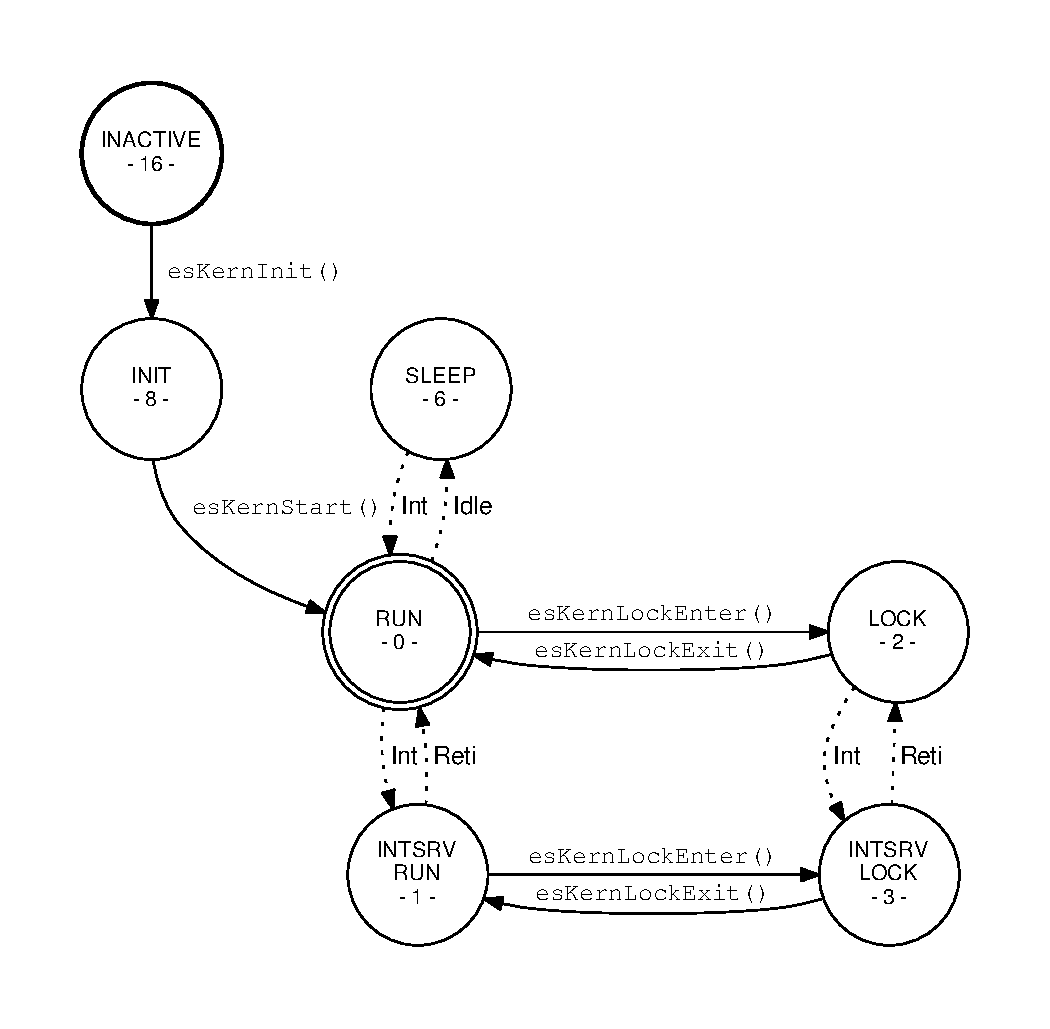
\includegraphics[width=\textwidth,height=\textheight/2,keepaspectratio=true]{dot_inline_dotgraph_1}}
\end{DoxyImageNoCaption}
\end{center}
 \begin{DoxyParagraph}{I\-N\-A\-C\-T\-I\-V\-E}
Inactive state of the kernel (Level 5). This state is entered after a physical reset. When the system is in this state all the maskable interrupt sources are disabled. In this state none of kernel internal data structures are initialized. In this state it is not possible to use any Kernel A\-P\-I except \hyperlink{group__kern__intf_ga9e9ff699d62d6035cd51121bb3140704}{es\-Kern\-Init()}.
\end{DoxyParagraph}
\begin{DoxyParagraph}{I\-N\-I\-T}
Initialization state of the kernel (Level 4). In this state all internal data structures are initialized but the kernel is still not running. In this stage new threads can be created by calling \hyperlink{group__kern__intf_gac91734f3ee867b519f59bf81cc7fde88}{es\-Thd\-Init()} function. Also, the application is allowed to use A\-P\-I which is used to create kernel structures like Thread Queues \hyperlink{structesThdQ}{es\-Thd\-Q}. All the maskable interrupt sources are D\-I\-S\-A\-B\-L\-E\-D.
\end{DoxyParagraph}
\begin{DoxyParagraph}{R\-U\-N}
Normal, running state of the kernel (Level 0). To start multi-\/threading just call the \hyperlink{group__kern__intf_ga0e7a0a6b9c02df58de0f98de0229a09d}{es\-Kern\-Start()} function. This function will switch the kernel into {\ttfamily R\-U\-N} state and multi-\/threading of created threads will commence. During the {\ttfamily R\-U\-N} state you are allowed to create other task as well. All the interrupt sources are enabled and the system A\-P\-Is are accessible, threads are running. All the maskable interrupt sources are E\-N\-A\-B\-L\-E\-D.
\end{DoxyParagraph}
\begin{DoxyParagraph}{L\-O\-C\-K}
Scheduler locked state, no context switching (Level 2). The running state of the kernel can be switched to {\ttfamily L\-O\-C\-K} state where the scheduler is locked and no context switching is allowed. {\ttfamily L\-O\-C\-K} state is one way of preventing the access to a shared resource. One more reason to lock the scheduler would be during the accessing of special hardware (e.\-g. programming the F\-L\-A\-S\-H memory) which does not allow interruption of the running operation. Usage of scheduler locks should be kept at minimum. All the maskable interrupt sources are E\-N\-A\-B\-L\-E\-D.
\end{DoxyParagraph}
\begin{DoxyParagraph}{I\-N\-T\-S\-R\-V\-\_\-\-R\-U\-N or I\-N\-T\-S\-R\-V\-\_\-\-L\-O\-C\-K}
Interrupt Service state, no context switching (Levels 1 and 3). During the both states {\ttfamily R\-U\-N} and {\ttfamily L\-O\-C\-K}, an interrupt event can occur. When Interrupt Service Routine is executing the kernel is in {\ttfamily I\-N\-T\-S\-R\-V\-\_\-\-R\-U\-N} or {\ttfamily I\-N\-T\-S\-R\-V\-\_\-\-L\-O\-C\-K} state. Each state corresponds to the state where the execution was interrupted from and the kernel will return to it's original state.
\end{DoxyParagraph}
\begin{DoxyParagraph}{S\-L\-E\-E\-P}
When idle condition occurs the kernel will switch to {\ttfamily S\-L\-E\-E\-P} state (if power saving is enabled). In order to return to {\ttfamily R\-U\-N} state an interrupt must occur whether from system timer or any other interrupt source which must request a context switch upon exit from I\-S\-R.
\end{DoxyParagraph}
\begin{DoxyNote}{Note}
The level of state {\ttfamily I\-N\-A\-C\-T\-I\-V\-E} is the highest. As the kernel boots up the level is decremented. The running state is level 0. 
\end{DoxyNote}

\section{Thread Management}
\label{threads}
\hypertarget{threads}{}
Introduction to threads and how to use them

\par
\par
\par
\hypertarget{threads_threads_intro}{}\subsection{Intro}\label{threads_threads_intro}
A thread, also called a thread of execution is the smallest sequence of program instructions that can be managed by an operating system scheduler. Multi-\/threading is implemented by time-\/division multiplexing where the processor switches between threads. Context switching occurs fast enough that the user perceives the threads as running at the same time. By using threads a programmer can split the work into the threads, each responsible for a smaller portion of the problem. From a threads view he thinks it has the processor all to itself.\hypertarget{threads_kern_threads}{}\subsubsection{e\-Solid R\-T Kernel thread}\label{threads_kern_threads}
e\-Solid R\-T Kernel supports multi-\/threading and allows applications to have any number of threads. The only limiting factors for the maximum number of threads are the amount of R\-A\-M and R\-O\-M memory and processing time.

Threads are implemented as normal {\ttfamily C} functions. Thread functions must have the following prototype\-:


\begin{DoxyCode}
\textcolor{keywordtype}{void} fn (\textcolor{keywordtype}{void} *);
\end{DoxyCode}


Which in plain english means\-: {\itshape fn is a function (pointer to void) returning void}.\hypertarget{threads_kern_threads_state}{}\subsubsection{Thread states}\label{threads_kern_threads_state}
A thread can be in one of the following states\-: \begin{center}

\begin{DoxyImageNoCaption}
  \mbox{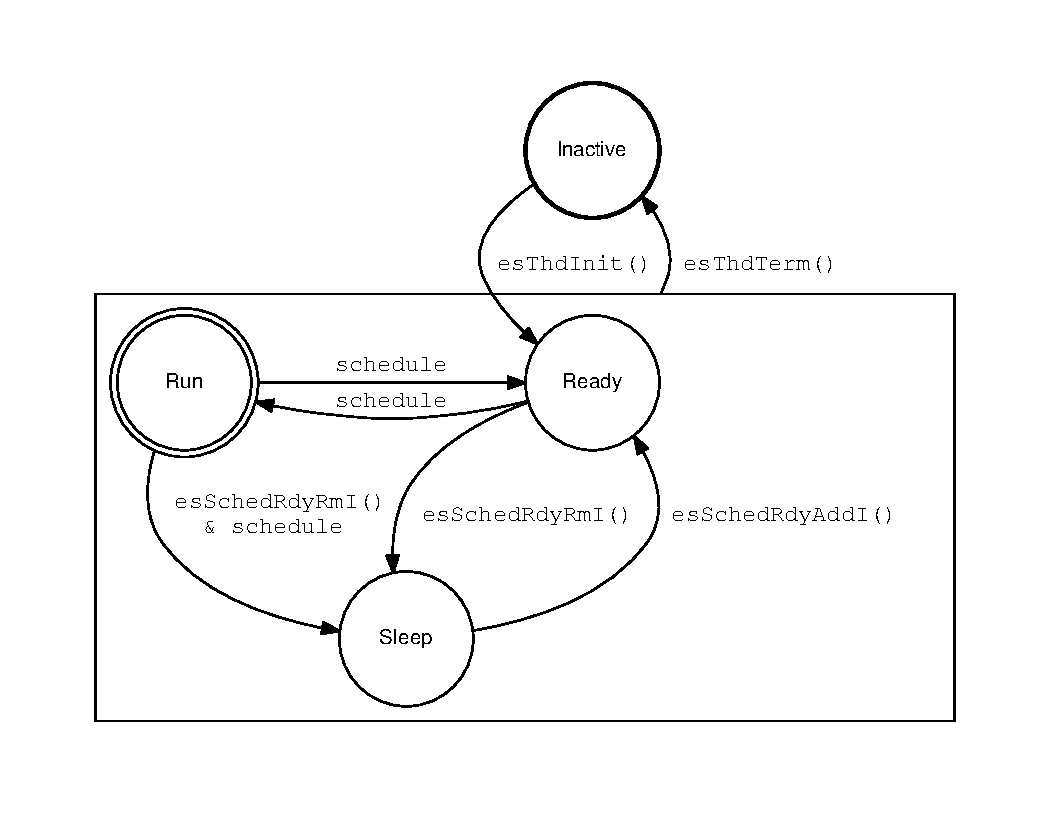
\includegraphics[width=\textwidth,height=\textheight/2,keepaspectratio=true]{dot_inline_dotgraph_2}}
\end{DoxyImageNoCaption}
\end{center}
 \begin{DoxyParagraph}{Inactive}
This is thread initial state. Threads in this state are still not activated ({\bfseries inactive}) by \hyperlink{group__kern__intf_gac91734f3ee867b519f59bf81cc7fde88}{es\-Thd\-Init()} function or they were deleted by \hyperlink{group__kern__intf_gac9d1eac76f26096614e8196bcfd8b905}{es\-Thd\-Term()} function. The scheduler does not recognize these threads and they will never execute.
\end{DoxyParagraph}
\begin{DoxyParagraph}{Ready}
Threads waiting to execute. There are the threads that are {\bfseries ready} to execute but are not currently executing because a different thread (equal or higher priority) is already executing.
\end{DoxyParagraph}
\begin{DoxyParagraph}{Run}
Thread is currently executing. When the thread is in this state then the code is actually being {\bfseries run} on the processor.
\end{DoxyParagraph}
\begin{DoxyParagraph}{Sleep}
Thread is sleeping. These threads are {\bfseries sleeping} while waiting for an event to occur.
\end{DoxyParagraph}
\hypertarget{threads_thd_create}{}\subsection{Initializing Threads}\label{threads_thd_create}
\hypertarget{threads_thd_create_init}{}\subsubsection{es\-Thd\-Init() A\-P\-I function}\label{threads_thd_create_init}
Threads are initialized by using \hyperlink{group__kern__intf_gac91734f3ee867b519f59bf81cc7fde88}{es\-Thd\-Init()} A\-P\-I function.

\begin{DoxyParagraph}{Stack size}

\end{DoxyParagraph}
There is no easy way to determine the stack size required by a thread. It is possible to calculate approximate stack size for simple threads, but for more complex ones (e.\-g. which calls library A\-P\-I function) this can be a daunting task. In this case stack size will be set to a size more than adequate for the thread and then use the profiling features provided by the kernel to ensure both that the space allocated is adequate, and that R\-A\-M space is not being unnecessarily wasted. 
\section{Critical sections}
\label{critical_section}
\hypertarget{critical_section}{}
How to deal with critical sections in an application\hypertarget{critical_section_cs_intro}{}\subsection{Intro}\label{critical_section_cs_intro}
In concurrent programming, a critical section is a piece of code that accesses a shared resource (data structure or device) that must not be concurrently accessed by more than one thread of execution. A critical section will usually terminate in fixed time, and a thread will have to wait for a fixed time to enter it (aka bounded waiting). Some synchronization mechanism is required at the entry and exit of the critical section to ensure exclusive use, for example a semaphore.\hypertarget{critical_section_kern_critical_sections}{}\subsubsection{e\-Solid -\/ R\-T Kernel internal critical sections}\label{critical_section_kern_critical_sections}
In contrast to application code in kernel code there is no other mechanism to protect critical code except disabling interrupts. Fortunately, some ports have ability to mask certain interrupts with low priority and allow interrupts with higher priority. By masking low priority interrupts the kernel can protect its critical sections. However for this scheme to work its forbidden to call any O\-S service function from a high priority interrupt. If this rule is not followed then the high priority interrupt with an O\-S service function call can preempt the kernel low priority interrupt which will in that case corrupt the kernel internal data structures.

\begin{DoxyNote}{Note}
1) It is forbidden to call any O\-S service function from an interrupt with the priority higher than the kernel interrupt priority. 

2) On some ports the kernel never completely disables interrupts.
\end{DoxyNote}
\hypertarget{critical_section_cs_implementation}{}\subsection{Implementation}\label{critical_section_cs_implementation}
There are multiple ways how are critical sections implemented\-:
\begin{DoxyItemize}
\item The simplest method is to prevent interrupts on entry into the critical section, and restoring interrupts to their previous state on exit from critical section. Any thread of execution entering any critical section anywhere in the system, with this implementation, will prevent any other thread, including an interrupt, from being executed on the C\-P\-U.
\item This approach can be improved upon by using semaphores. To enter a critical section, a thread must obtain a semaphore, which it releases on leaving the section. Other threads are prevented from entering the critical section at the same time as the original thread, but are free to gain control of the C\-P\-U and execute other code, including other critical sections that are protected by different semaphores.
\end{DoxyItemize}\hypertarget{critical_section_cs_interrupt_lock}{}\subsubsection{Disabling interrupts}\label{critical_section_cs_interrupt_lock}
In order to properly disable interrupts the application must follow these steps\-:
\begin{DoxyItemize}
\item declare an {\ttfamily auto} variable which will hold interrupt state
\item save interrupt status into {\ttfamily auto} variable and disable interrupts
\item access the shared resource
\item restore previously saved interrupt state
\end{DoxyItemize}

The {\ttfamily auto} variable must be of portable type {\ttfamily port\-Reg\-\_\-\-T}. This variable will hold temporary interrupt status. Then by using the macro {\ttfamily E\-S\-\_\-\-C\-R\-I\-T\-I\-C\-A\-L\-\_\-\-L\-O\-C\-K\-\_\-\-E\-N\-T\-E\-R()} the state of enabled interrupts will be saved in interrupt context variable declared earlier. Immediately after saving the interrupt state the macro will lock interrupts. Now the code can safely access and use the shared resource. When code finishes using the resource it will call {\ttfamily E\-S\-\_\-\-C\-R\-I\-T\-I\-C\-A\-L\-\_\-\-L\-O\-C\-K\-\_\-\-E\-X\-I\-T()} macro. This macro will restore interrupts from the previously saved interrupt state.


\begin{DoxyCode}
portReg\_T intCtx;                   \textcolor{comment}{/* Declare an interrupt context status variable */}
    :
    :
    :
ES\_CRITICAL\_LOCK\_ENTER(&intCtx);    \textcolor{comment}{/* Save state and lock interrupts */}
\textcolor{comment}{/*}
\textcolor{comment}{ * Access the shared resource}
\textcolor{comment}{ */}
ES\_CRITICAL\_LOCK\_EXIT(intCtx);      \textcolor{comment}{/* Restore previous state unlocking the interrupts */}
\end{DoxyCode}
 \begin{DoxyParagraph}{When to use this scheme}

\begin{DoxyItemize}
\item If interrupt service routine {\itshape changes} the shared resource state.
\item If the processing time of critical section is very small.
\end{DoxyItemize}
\end{DoxyParagraph}
\begin{DoxyParagraph}{When not to use this scheme}

\begin{DoxyItemize}
\item If interrupt service routine takes a lot of C\-P\-U time to process critical section do not use this method. If a critical section is long, then the system clock will drift every time a critical section is executed because the system timer interrupt can not be serviced. Also, if a program execution halts during its critical section, control will never be returned to another thread, effectively halting the entire system.
\end{DoxyItemize}
\end{DoxyParagraph}
\begin{DoxyNote}{Note}
Context switching is disabled during critical code section execution.
\end{DoxyNote}
\hypertarget{critical_section_cs_kernel_lock}{}\subsubsection{Disabling Kernel scheduler}\label{critical_section_cs_kernel_lock}
Another way to deal with a critical section and protect your shared resource is by locking the kernel scheduler. The kernel locking can be used only if you know that protected data will be modified only by other threads. This protection scheme can not be used when data is modified by interrupt service routines.


\begin{DoxyCode}
\hyperlink{group__kern__lock_ga86ec4f4cbaa889b0f23c7e2ebdcbbb97}{esKernLockEnter}();                  \textcolor{comment}{/* Temporarily disable kernel scheduler  */}
\textcolor{comment}{/*}
\textcolor{comment}{ * Access the shared resource}
\textcolor{comment}{ */}
\hyperlink{group__kern__lock_gaf1eec663f7cc5c414b113901382ccd82}{esKernLockExit}();                   \textcolor{comment}{/* Enable kernel scheduler */}
\end{DoxyCode}
 \begin{DoxyParagraph}{When to use this scheme}

\begin{DoxyItemize}
\item If interrupt service routine {\itshape never changes} the shared resource state.
\item If the processing time of critical section is very small.
\end{DoxyItemize}
\end{DoxyParagraph}
\begin{DoxyParagraph}{When not to use this scheme}

\begin{DoxyItemize}
\item If interrupt service routine takes a lot of C\-P\-U time to process critical section do not use this method. If a critical section is long, then the system will be {\itshape partially} unresponsive to other events since interrupt service routines can be invoked, but note that any further processing by other threads is still disabled.
\end{DoxyItemize}
\end{DoxyParagraph}
\hypertarget{critical_section_cs_sem_lock}{}\subsubsection{Using semaphores}\label{critical_section_cs_sem_lock}

\section{Time complexity}
\label{time_complexity}
\hypertarget{time_complexity}{}
About time categories of algorithms\hypertarget{time_complexity_tc_intro}{}\subsection{Intro}\label{time_complexity_tc_intro}
In computer science, the time complexity of an algorithm quantifies the amount of time taken by an algorithm to run as a function of the length of the input. The time complexity of an algorithm is commonly expressed using {\bfseries big O} notation, which excludes coefficients and lower order terms. When expressed this way, the time complexity is said to be described asymptotically, i.\-e., as the input size goes to infinity. For example, if the time required by an algorithm on all inputs of size {\ttfamily n} is at most {\ttfamily 5n$^\wedge$3 + 3n}, the asymptotic time complexity is {\ttfamily O(n$^\wedge$3)}.

Time complexity is commonly estimated by counting the number of elementary operations performed by the algorithm, where an elementary operation takes a fixed amount of time to perform. Thus the amount of time taken and the number of elementary operations performed by the algorithm differ by at most a constant factor.

Since an algorithm’s performance time may vary with different inputs of the same size, one commonly uses the worst-\/case time complexity of an algorithm, denoted as {\bfseries T(n)}, which is defined as the maximum amount of time taken on any input of size {\ttfamily n}. Time complexities are classified by the nature of the function {\ttfamily T(n)}. For instance, an algorithm with {\ttfamily T(n) = O(n)} is called a linear time algorithm, and an algorithm with {\ttfamily T(n) = O(2$^\wedge$n)} is said to be an exponential time algorithm.

\begin{DoxyNote}{Note}
Worst-\/case time-\/complexity {\ttfamily T(n)} indicates the longest running time performed by an algorithm given any input of size {\ttfamily n}, and thus this guarantees that the algorithm finishes on time.
\end{DoxyNote}
\hypertarget{time_complexity_tc_big_o}{}\subsubsection{Big O notation}\label{time_complexity_tc_big_o}
Big O notation describes the limiting behavior of a function when the argument tends towards a particular value or infinity, usually in terms of simpler functions and it is used to classify algorithms by how they respond (e.\-g., in their processing time or working space requirements) to changes in input size.\hypertarget{time_complexity_tc_constant_time}{}\subsection{Constant time}\label{time_complexity_tc_constant_time}
An algorithm is said to be constant time (also written as {\ttfamily O(1)} time) if the value of {\ttfamily T(n)} is bounded by a value that does not depend on the size of the input.

Despite the name {\itshape constant time}, the running time does not have to be independent of the problem size, but an upper bound for the running time has to be bounded independently of the problem size.

\begin{DoxyNote}{Note}
Constant time effectively means that there is a constant upper bound to how long the function will take to run which isn’t affected by any of the input argument.
\end{DoxyNote}
\hypertarget{time_complexity_tc_esolid}{}\subsubsection{e\-Solid -\/ R\-T Kernel time complexity}\label{time_complexity_tc_esolid}
All e\-Solid -\/ R\-T Kernel functions are using {\ttfamily constant time O(1)} algorithms. This is especially important for Real Time applications. 
\section{Scheduler}
\label{scheduler}
\hypertarget{scheduler}{}
About the scheduler and Ready Threads Queue\hypertarget{scheduler_sched_quantum}{}\subsection{Quantum}\label{scheduler_sched_quantum}
The period of time for which a thread is allowed to execute in a preemptive multi-\/threading system is generally called the time slice, or {\ttfamily quantum}. The scheduler is run once every quantum to choose the next thread for execution. If the quantum is too short then the scheduler overhead may become high.

An interrupt is used to allow the kernel to switch between threads when their quantum expires, effectively allowing the processor's time to be shared between a number of threads, giving the illusion that it is dealing with these threads concurrently.\hypertarget{scheduler_sched_thdL}{}\subsection{Threads List}\label{scheduler_sched_thdL}
Each thread structure \hyperlink{structesThd}{es\-Thd} contains Thread List structure \hyperlink{structesThd_a69f72ac3b1f6199da48b41804f353325}{es\-Thd\-::thd\-L}. All threads of the same priority are linked together via {\itshape next} and {\itshape prev} members in \hyperlink{structesThd_a69f72ac3b1f6199da48b41804f353325}{es\-Thd\-::thd\-L} structure. The first member of the structure is pointer {\itshape q} which points back to the Threads Queue structure (\hyperlink{structesThdQ}{es\-Thd\-Q}) which contains the threads.

The list is organized as {\bfseries circular doubly linked list}, which means that {\itshape tail} and {\itshape head} nodes are linked together just like every other node in the list. This provides easy and efficient traversal of the list.


\begin{DoxyImage}
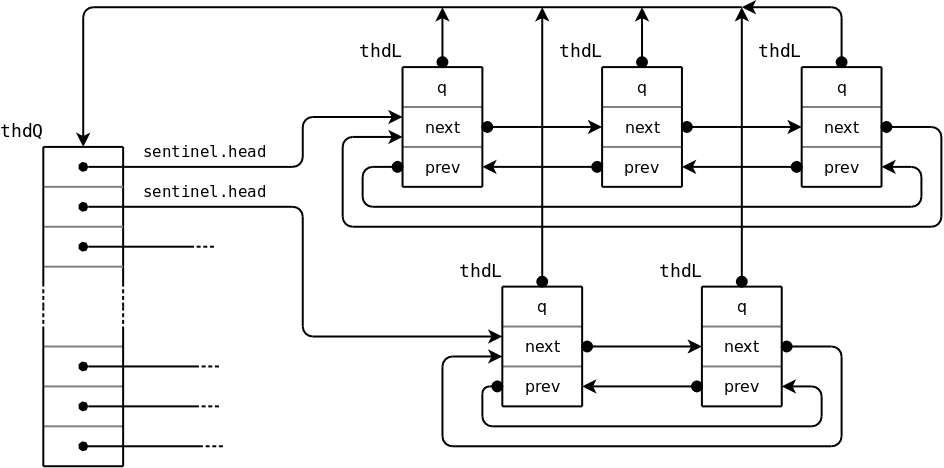
\includegraphics[width=12cm]{thdL.png}
\caption{Detailed view of Threads List (sentinel.next pointers not shown)}
\end{DoxyImage}


Each sentinel of a list has two pointers, {\itshape head} and {\itshape next}. Pointer sentinel.\-head$\ast$ always points to the first entry of the list which is called head$\ast$. Every new thread is added at the {\itshape tail} of the list which is essentialy just after the node {\itshape head}. When a first thread is added to the list the pointer sentinel.\-next$\ast$ points to the thread, too. When the list is rotated using function \hyperlink{group__kern__thdq_gae365b14292f1496a90d876baec84fb4e}{es\-Thd\-Q\-Fetch\-Rotate\-I()} the pointer {\itshape sentinel.\-next} is advanced forward and points to the next thread in list.


\begin{DoxyImage}
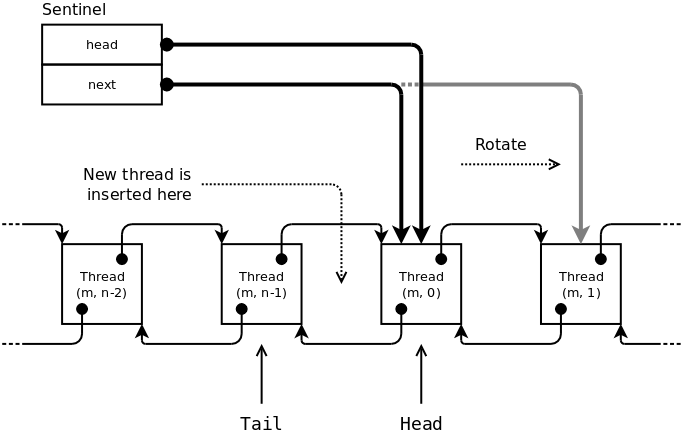
\includegraphics[width=12cm]{thdL-rotate.png}
\caption{Detailed view of the sentinel and linked list}
\end{DoxyImage}
\hypertarget{scheduler_sched_thdQ}{}\subsection{Threads Queue}\label{scheduler_sched_thdQ}
Based on the number of configured priority levels (see \hyperlink{group__template__kern__cfg_ga56bd89fe76f7fe22f3d8805bc3c68892}{C\-F\-G\-\_\-\-S\-C\-H\-E\-D\-\_\-\-P\-R\-I\-O\-\_\-\-L\-V\-L}) and on the number of data register bits (see {\ttfamily P\-O\-R\-T\-\_\-\-D\-E\-F\-\_\-\-D\-A\-T\-A\-\_\-\-W\-I\-D\-T\-H}) of the used C\-P\-U, two configurations are possible\-:
\begin{DoxyItemize}
\item Simple Ready Threads Queue
\item Complex Ready Threads Queue
\end{DoxyItemize}

Simple Ready Threads Queue configuration is used when the number of configured priority levels is lower or equal to the number of bits in general purpose data register. For example if application is using 9 priority levels on 32-\/bit C\-P\-U than simple Ready Threads Queue configuration is used. In contrast, when using 9 priority levels on an 8-\/bit C\-P\-U than the kernel is forced to use the Complex Ready Threads Queue configuration since 8-\/bit register cannot carry 9 bits of data.\hypertarget{scheduler_sched_rdyThdQ_simple}{}\subsubsection{Simple Ready Threads Queue}\label{scheduler_sched_rdyThdQ_simple}
Each bit in {\ttfamily bit\mbox{[}0\mbox{]}} variable represents one priority level. The number of bits used in this variable depends on \hyperlink{group__template__kern__cfg_ga56bd89fe76f7fe22f3d8805bc3c68892}{C\-F\-G\-\_\-\-S\-C\-H\-E\-D\-\_\-\-P\-R\-I\-O\-\_\-\-L\-V\-L} value. If a bit at {\ttfamily Nth} position is set then there is a thread inserted in Thread List at {\ttfamily Nth} priority level.

\par

\begin{DoxyImage}
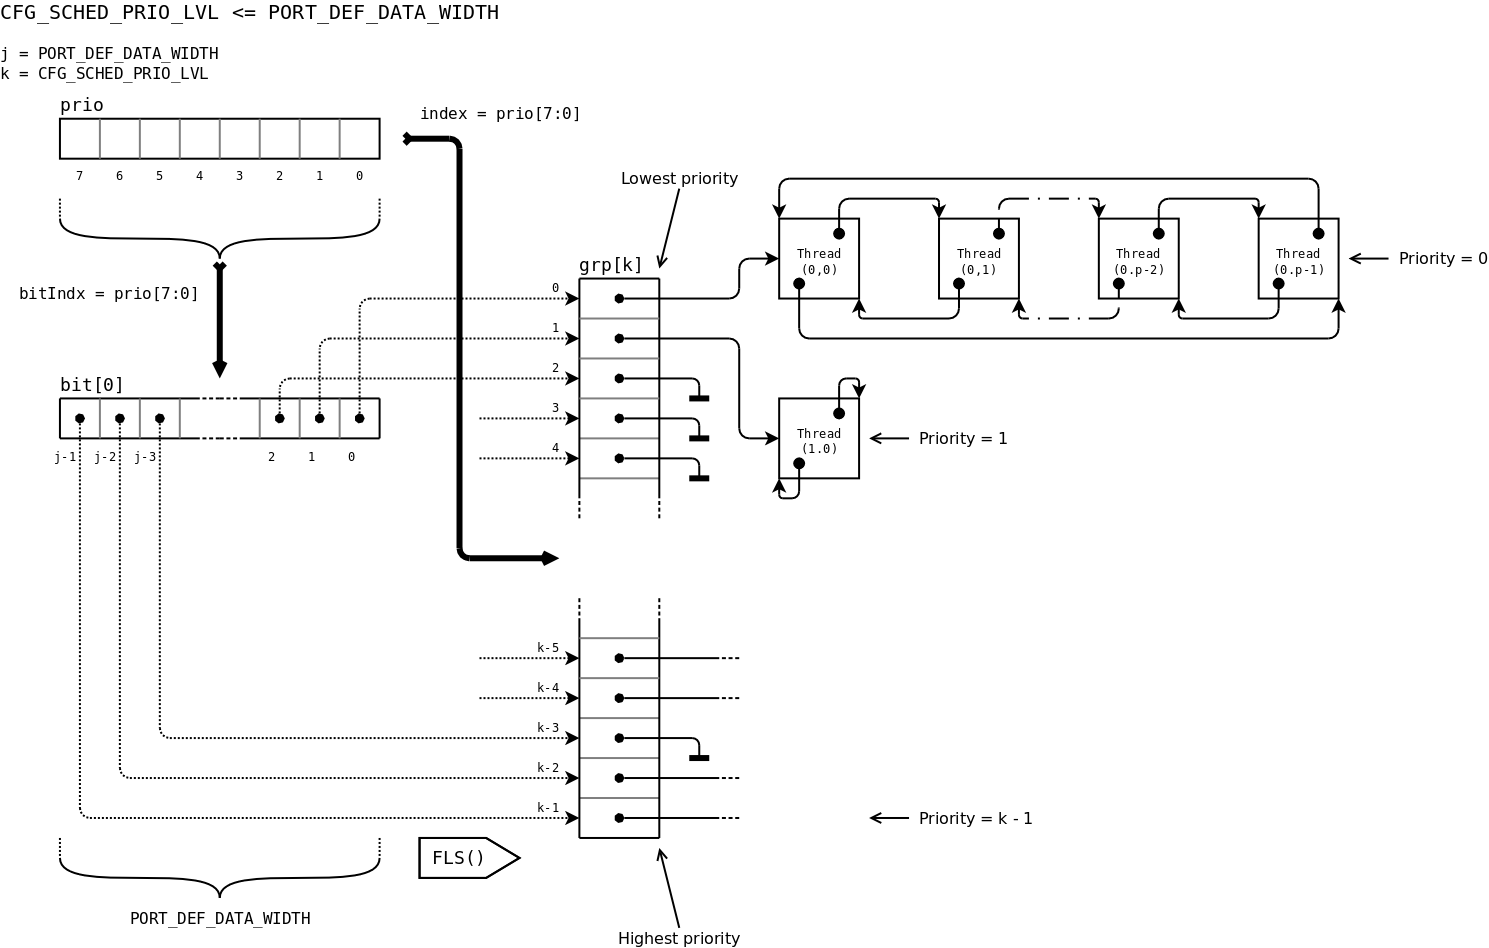
\includegraphics[width=15cm]{thdQ-simple.png}
\caption{Ready Threads Queue -\/ low number of priority levels}
\end{DoxyImage}


\begin{DoxyParagraph}{Inserting a thread}
The process of a thread insertion into a thread queue can be described using the following pseudo-\/code\-: 
\begin{DoxyCode}
\textcolor{keyword}{function} insert(thread)
    priority := thread.priority                             \textcolor{preprocessor}{# Get the priority of the thread}
\textcolor{preprocessor}{}
    \textcolor{keywordflow}{if} (grp[priority].head == NULL)                         # If \textcolor{keyword}{this} priority level has a list
        grp[priority].head := thread                        # Create a list with \textcolor{keyword}{this} thread as head
        grp[priority].next := thread
        bitIndx := 2^priority                               # bitIndx equals to 2 raised to the power of 
      priority
        bit[0]  := bit[0] or bitIndx                        # Set the calculated bit in Bit Map
    \textcolor{keywordflow}{else}
        listInsertAtTail(grp[priority].head, thread)        \textcolor{preprocessor}{# Add thread at tail of existing list}
\textcolor{preprocessor}{}    end \textcolor{keywordflow}{if}
end \textcolor{keyword}{function}
\end{DoxyCode}

\end{DoxyParagraph}
\begin{DoxyParagraph}{Removing a thread}
The process of a thread removal can be described with the following pseudo-\/code\-: 
\begin{DoxyCode}
\textcolor{keyword}{function} \textcolor{keyword}{remove}(thread)
    priority := thread.priority                             # Get the priority of the thread

    if (listIsEntryLast(thread))                            # In \textcolor{keywordflow}{case} we are removing the last entry
        grp[priority].head := NULL                          # List is deleted
        bitIndx := 2^priority                               # bitIndx equals to 2 raised to the power of 
      priority
        bit[0]  := bit[0] and not bitIndx                   # Clear the calculated bit in Bit Map
    \textcolor{keywordflow}{else}
        listRemove(thread)                                  # Remove the thread from list
    end \textcolor{keywordflow}{if}
end \textcolor{keyword}{function}
\end{DoxyCode}

\end{DoxyParagraph}
\begin{DoxyParagraph}{Fetching the highest priority thread}
The process of fetching the highest priority thread is inverse function of {\ttfamily 2$^\wedge$priority} which was used in {\ttfamily insert()} function\-: 
\begin{DoxyCode}
\textcolor{keyword}{function} fetch()
    priority := log2(bit[0])                                \textcolor{preprocessor}{# Find Last Set bit position in bit[0]}
\textcolor{preprocessor}{}
    \textcolor{keywordflow}{return} grp[priority]
end \textcolor{keyword}{function}
\end{DoxyCode}

\end{DoxyParagraph}
\begin{DoxyParagraph}{Rotating the threads queue}
The process can be described with the following algorithm\-: 
\begin{DoxyCode}
\textcolor{keyword}{function} rotate()
    priority := log2(bit[0])                                \textcolor{preprocessor}{# Find Last Set bit position in bit[0]}
\textcolor{preprocessor}{}
    grp[priority].next := grp[priority].next.next

    \textcolor{keywordflow}{return} grp[priority].next
end \textcolor{keyword}{function}
\end{DoxyCode}
 
\end{DoxyParagraph}
\hypertarget{scheduler_sched_rdyThdQ_complex}{}\subsubsection{Complex Ready Threads Queue}\label{scheduler_sched_rdyThdQ_complex}

\begin{DoxyImage}
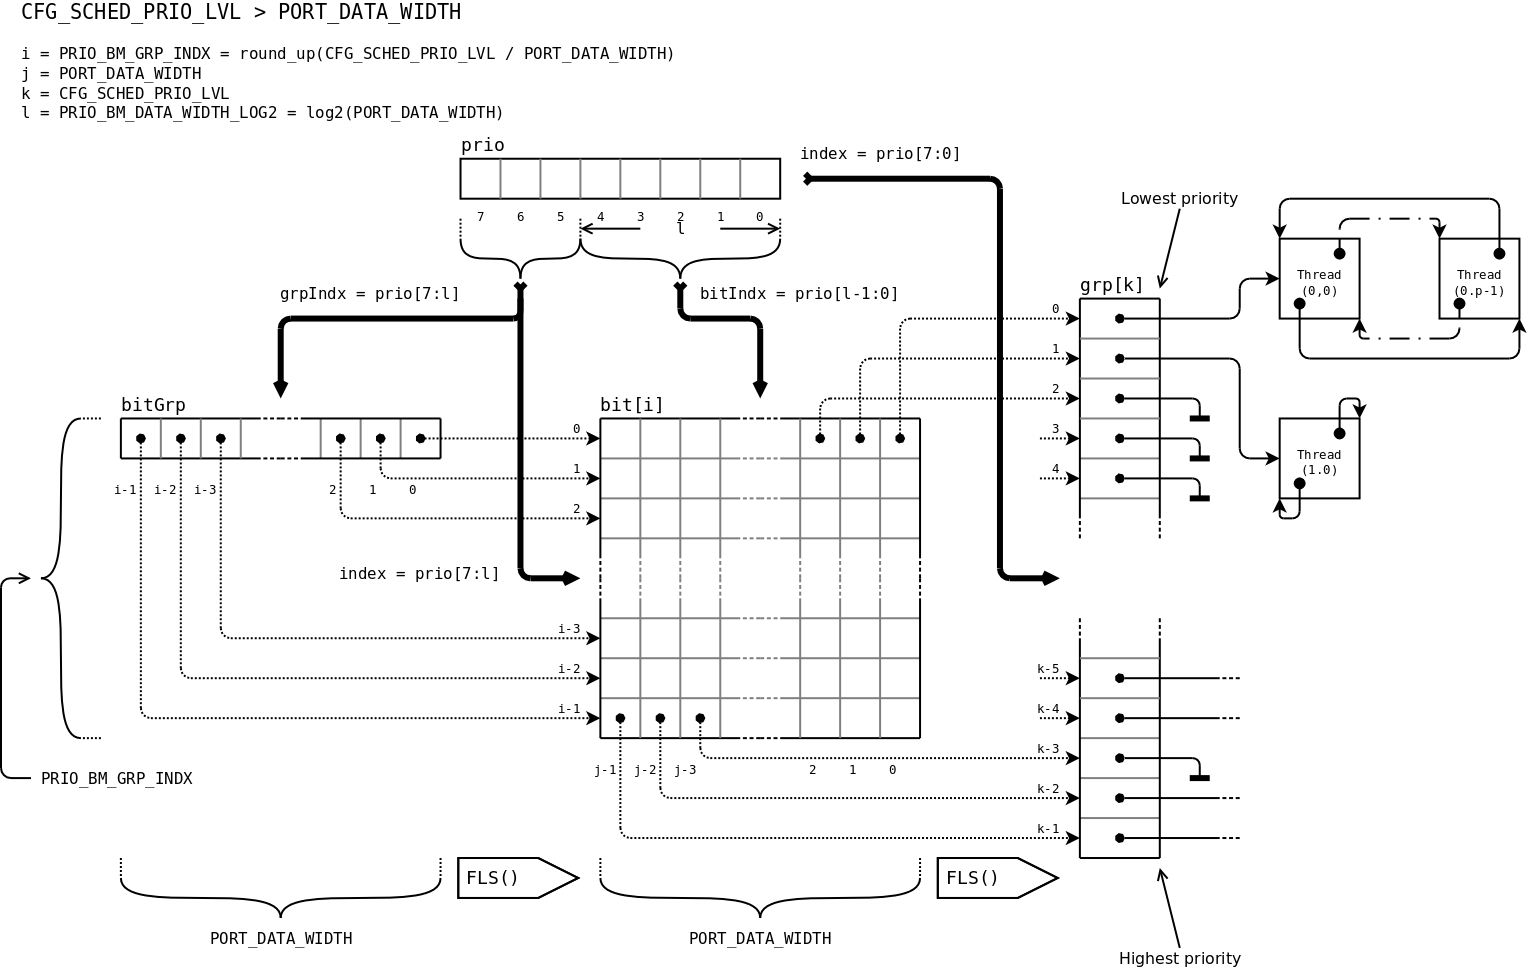
\includegraphics[width=17cm]{thdQ-complex.png}
\caption{Ready Threads Queue -\/ high number of priority levels}
\end{DoxyImage}
\hypertarget{scheduler_sched_rdyThdQ}{}\subsection{Ready Threads Queue}\label{scheduler_sched_rdyThdQ}
Ready Threads Queue holds threads that are ready for execution. 
\section{Change Log}
\label{changelog}
\hypertarget{changelog}{}
Brief change log

2013-\/07-\/03 Nenad Radulovic


\begin{DoxyItemize}
\item {\ttfamily N\-E\-W\-:} Initial implementation of system timer
\item {\ttfamily N\-E\-W\-:} Initial implementation of power savings features
\item {\ttfamily U\-P\-D\-A\-T\-E\-:} Many functions have full A\-P\-I contract restrictions
\end{DoxyItemize}

2013-\/05-\/28 Nenad Radulovic


\begin{DoxyItemize}
\item {\ttfamily N\-E\-W\-:} Initial project import
\item {\ttfamily N\-E\-W\-:} Initial commit
\item {\ttfamily U\-P\-D\-A\-T\-E\-:} Eclipse project files are added to gitignore 
\end{DoxyItemize}
\section{Abbreviations}
\label{abbreviation}
\hypertarget{abbreviation}{}
Common abbreviations used in code

\begin{TabularC}{2}
\hline
\rowcolor{lightgray}{\bf Word }&{\bf Abbreviation  }\\\cline{1-2}
interrupt &intr \\\cline{1-2}
interrupt service routine &isr \\\cline{1-2}
interrupt request &irq \\\cline{1-2}
priority &prio \\\cline{1-2}
stack &stck \\\cline{1-2}
system &sys \\\cline{1-2}
thread &thd \\\cline{1-2}
timer &tmr \\\cline{1-2}
queue &q \\\cline{1-2}
virtual &v \\\cline{1-2}
\end{TabularC}

\section{Quick-\/start guide}
\label{md__home_nenad_git_nradulovic_esolid-kernel_README}
\hypertarget{md__home_nenad_git_nradulovic_esolid-kernel_README}{}
This is a bare-\/kernel, the result of two weeks of work. It is intended for a bigger project which already includes some synchronization mechanisms. The initial idea was that this kernel would only provide minimal functionality for context switching, but the kernel implementation went so nicely that I think that it would be great to share it.

e\-Solid is a collection of resources for embedded system design and this Real-\/\-Time kernel is only a piece of that collection. Because of that fact remember\-: {\itshape there are (still) no synchronization or I\-P\-C mechanisms in this kernel}, and it can be viewed as a preemptive Round-\/\-Robin scheduler, only.

\subsubsection*{T\-O\-D\-O list}


\begin{DoxyItemize}
\item Integrate a profiling system (memory/stack usage, cpu usage...)
\item test, test, test...
\end{DoxyItemize}

\subsection*{Using e\-Solid -\/ Real-\/\-Time Kernel}

\subsubsection*{Configuration and ports}

Configuration is done in two files\-: {\ttfamily \hyperlink{kernel__cfg_8h}{kernel\-\_\-cfg.\-h}} (port independent settings) and in {\ttfamily cpu\-\_\-cfg.\-h} (port depended settings, located in port structure). Currently, kernel is ported only to A\-R\-Mv7-\/\-M architecture range of microcontrollers. It was tested on S\-T\-M32\-F100 series of microcontrollers, but it should work, with minimal modifications, on any A\-R\-Mv7-\/\-M C\-P\-U. Some other ports like A\-V\-R-\/\-G\-C\-C are planned, too.

\subsubsection*{Building}

The kernel was built using arm-\/none-\/eabi G\-C\-C v4.\-7.\-3 compiler toolchain (from \href{https://launchpad.net/gcc-arm-embedded/+download}{\tt https\-://launchpad.\-net/gcc-\/arm-\/embedded/+download}) and binary was downloaded to the M\-C\-U using {\itshape texane} gdb-\/server. There are no makefiles, it is assumed that I\-D\-E will generate them for you.

\subparagraph*{Example for S\-T\-M32\-F10x family port}

There are two groups of source files which need to be compiled for A\-R\-Mv7-\/\-M architecture\-:
\begin{DoxyItemize}
\item \hyperlink{kernel_8c}{kernel.\-c}, semaphore.\-c, dbg.\-c in {\ttfamily ./src} source directory and
\item cpu.\-c in {\ttfamily ./port/arm-\/none-\/eabi-\/gcc/v7-\/m} port directory.
\end{DoxyItemize}

The following include paths are needed\-:
\begin{DoxyItemize}
\item {\ttfamily ./inc}
\item {\ttfamily ./port/arm-\/none-\/eabi-\/gcc/common}
\item {\ttfamily ./port/arm-\/none-\/eabi-\/gcc/v7-\/m}
\item {\ttfamily ./port/arm-\/none-\/eabi-\/gcc/stm32f10x}
\end{DoxyItemize}

\subsubsection*{Documentation}

Some documentation is available under Wiki \href{https://github.com/nradulovic/esolid-kernel/wiki}{\tt https\-://github.\-com/nradulovic/esolid-\/kernel/wiki}. Doxygen configuration and full documentation source files are available in {\ttfamily /doc} directory. Go to the directory {\ttfamily doc} create a directory named {\ttfamily kernel} and than run doxygen\-: \begin{DoxyVerb}# doxygen doxyfile-kernel
# doxygen doxyfile-kernel-port
\end{DoxyVerb}


This will generate H\-T\-M\-L, La\-Tex and man documentation in {\ttfamily ./doc/kernel} and {\ttfamily ./doc/kernel-\/port} directories, respectively.

\subsubsection*{Running}

To successfully use and run kernel you will need to study the kernel documentation. The documentation is still being written and some examples will be added later. 
\section{Todo List}
\label{todo}
\hypertarget{todo}{}

\begin{DoxyRefList}
\item[\label{todo__todo000002}%
\hypertarget{todo__todo000002}{}%
Global \hyperlink{group__template__cpu__intf_ga31d47ffb78c3755575e66821b3a72a62}{P\-O\-R\-T\-\_\-\-D\-E\-F\-\_\-\-K\-I\-D\-L\-E\-\_\-\-S\-T\-C\-K\-\_\-\-S\-I\-Z\-E} ]This value needs tweaking  
\item[\label{todo__todo000001}%
\hypertarget{todo__todo000001}{}%
Global \hyperlink{group__template__cpu__intf_gabaa296d76c28043a60531ad8ed81504b}{P\-O\-R\-T\-\_\-\-D\-E\-F\-\_\-\-K\-V\-T\-M\-R\-\_\-\-S\-T\-C\-K\-\_\-\-S\-I\-Z\-E} ]This value needs tweaking 
\end{DoxyRefList}
\section{Module Documentation}
\hypertarget{group__kern__sync}{\subsection{Synchronization services}
\label{group__kern__sync}\index{Synchronization services@{Synchronization services}}
}


Basic synchronization services.  


Collaboration diagram for Synchronization services\-:\nopagebreak
\begin{figure}[H]
\begin{center}
\leavevmode
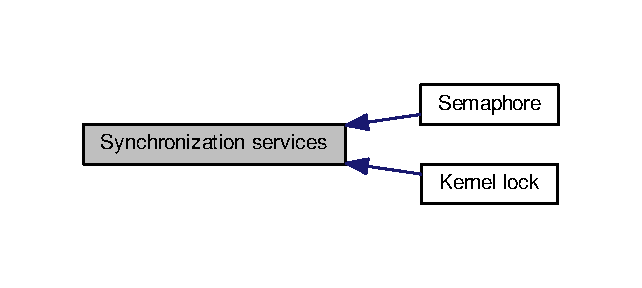
\includegraphics[width=308pt]{group__kern__sync}
\end{center}
\end{figure}
\subsubsection*{Modules}
\begin{DoxyCompactItemize}
\item 
\hyperlink{group__lock__intf}{Kernel lock}
\begin{DoxyCompactList}\small\item\em Kernel locking. \end{DoxyCompactList}\item 
\hyperlink{group__sem__intf}{Semaphore}
\begin{DoxyCompactList}\small\item\em Counting semaphore. \end{DoxyCompactList}\end{DoxyCompactItemize}


\subsubsection{Detailed Description}
Basic synchronization services. 
\hypertarget{group__lock__intf}{\subsection{Kernel lock}
\label{group__lock__intf}\index{Kernel lock@{Kernel lock}}
}


Kernel locking.  


Collaboration diagram for Kernel lock\-:\nopagebreak
\begin{figure}[H]
\begin{center}
\leavevmode
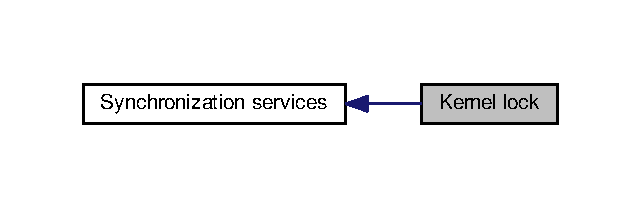
\includegraphics[width=308pt]{group__lock__intf}
\end{center}
\end{figure}
Kernel locking. The simplest method to protect a shared resource is by using kernel locks. For details see \hyperlink{group__kern__lock}{Kernel lock}. 
\hypertarget{group__sem__intf}{\subsection{Semaphore}
\label{group__sem__intf}\index{Semaphore@{Semaphore}}
}


Counting semaphore.  


Collaboration diagram for Semaphore\-:\nopagebreak
\begin{figure}[H]
\begin{center}
\leavevmode
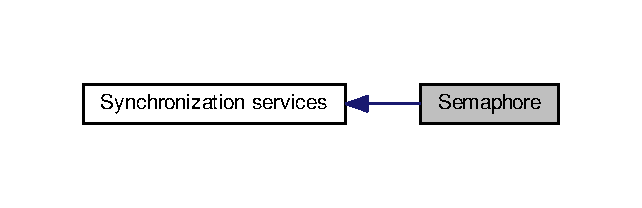
\includegraphics[width=308pt]{group__sem__intf}
\end{center}
\end{figure}
\subsubsection*{Data types group}
\label{_amgrpca30459c90d6b7a12b3df0a1317e654e}%
brief description \begin{DoxyCompactItemize}
\item 
\hypertarget{group__sem__intf_gaa080a10f59ad14ffb1e27d577b10e870}{typedef C\-F\-G\-\_\-\-S\-E\-M\-A\-P\-H\-O\-R\-E\-\_\-\-C\-N\-T\-\_\-\-T {\bfseries es\-Sem\-Cnt\-\_\-\-T}}\label{group__sem__intf_gaa080a10f59ad14ffb1e27d577b10e870}

\item 
\hypertarget{group__sem__intf_ga076de09738f0febcd417f15a9ac15a7e}{typedef struct es\-Sem {\bfseries es\-Sem\-\_\-\-T}}\label{group__sem__intf_ga076de09738f0febcd417f15a9ac15a7e}

\item 
\hypertarget{group__sem__intf_gaf38e40d531c3eb3d03ab29c0a116b235}{\#define {\bfseries C\-F\-G\-\_\-\-S\-E\-M\-A\-P\-H\-O\-R\-E\-\_\-\-C\-N\-T\-\_\-\-T}~int16\-\_\-t}\label{group__sem__intf_gaf38e40d531c3eb3d03ab29c0a116b235}

\end{DoxyCompactItemize}
\subsubsection*{Function group}
\label{_amgrpec1f4104dc63801ceee35db9d6f5502d}%
brief description \begin{DoxyCompactItemize}
\item 
void \hyperlink{group__sem__intf_gae4481945af3c671b99e87b151de98085}{es\-Sem\-Init} (es\-Sem\-\_\-\-T $\ast$sem, es\-Sem\-Cnt\-\_\-\-T cnt)
\begin{DoxyCompactList}\small\item\em Initialize a semaphore. \end{DoxyCompactList}\item 
\hypertarget{group__sem__intf_ga897ad9e48bcf3fea3fa68897cbcf33d9}{void {\bfseries es\-Sem\-Term} (es\-Sem\-\_\-\-T $\ast$sem)}\label{group__sem__intf_ga897ad9e48bcf3fea3fa68897cbcf33d9}

\item 
void \hyperlink{group__sem__intf_gaf742af1a3888b602a45e4cd394f28550}{es\-Sem\-Wait} (es\-Sem\-\_\-\-T $\ast$sem)
\begin{DoxyCompactList}\small\item\em Wait on a semaphore. \end{DoxyCompactList}\item 
void \hyperlink{group__sem__intf_ga4f11d79edca489a754f9385ca7c89b36}{es\-Sem\-Wait\-Timeout} (es\-Sem\-\_\-\-T $\ast$sem, \hyperlink{group__kern__vtmr_ga844873888c186ee81eb66620dadb0451}{es\-Tick\-\_\-\-T} time)
\begin{DoxyCompactList}\small\item\em Wait on a semaphore. \end{DoxyCompactList}\item 
void \hyperlink{group__sem__intf_ga372df852afd413b4fe2e65591da2fe79}{es\-Sem\-Post} (es\-Sem\-\_\-\-T $\ast$sem)
\begin{DoxyCompactList}\small\item\em Increment the value of a semaphore. \end{DoxyCompactList}\end{DoxyCompactItemize}


\subsubsection{Detailed Description}
Counting semaphore. 

\subsubsection{Function Documentation}
\hypertarget{group__sem__intf_gae4481945af3c671b99e87b151de98085}{\index{Semaphore@{Semaphore}!es\-Sem\-Init@{es\-Sem\-Init}}
\index{es\-Sem\-Init@{es\-Sem\-Init}!Semaphore@{Semaphore}}
\paragraph[{es\-Sem\-Init}]{\setlength{\rightskip}{0pt plus 5cm}void es\-Sem\-Init (
\begin{DoxyParamCaption}
\item[{es\-Sem\-\_\-\-T $\ast$}]{sem, }
\item[{es\-Sem\-Cnt\-\_\-\-T}]{cnt}
\end{DoxyParamCaption}
)}}\label{group__sem__intf_gae4481945af3c671b99e87b151de98085}


Initialize a semaphore. 


\begin{DoxyParams}{Parameters}
{\em sem} & Semaphore\-: points to a semaphore object to initialize. \\
\hline
{\em cnt} & Count\-: is an initial value to set the semaphore to. \\
\hline
\end{DoxyParams}
\hypertarget{group__sem__intf_gaf742af1a3888b602a45e4cd394f28550}{\index{Semaphore@{Semaphore}!es\-Sem\-Wait@{es\-Sem\-Wait}}
\index{es\-Sem\-Wait@{es\-Sem\-Wait}!Semaphore@{Semaphore}}
\paragraph[{es\-Sem\-Wait}]{\setlength{\rightskip}{0pt plus 5cm}void es\-Sem\-Wait (
\begin{DoxyParamCaption}
\item[{es\-Sem\-\_\-\-T $\ast$}]{sem}
\end{DoxyParamCaption}
)}}\label{group__sem__intf_gaf742af1a3888b602a45e4cd394f28550}


Wait on a semaphore. 


\begin{DoxyParams}{Parameters}
{\em sem} & Semaphore\-: points to a semaphore object to initialize. \\
\hline
\end{DoxyParams}
\hypertarget{group__sem__intf_ga4f11d79edca489a754f9385ca7c89b36}{\index{Semaphore@{Semaphore}!es\-Sem\-Wait\-Timeout@{es\-Sem\-Wait\-Timeout}}
\index{es\-Sem\-Wait\-Timeout@{es\-Sem\-Wait\-Timeout}!Semaphore@{Semaphore}}
\paragraph[{es\-Sem\-Wait\-Timeout}]{\setlength{\rightskip}{0pt plus 5cm}void es\-Sem\-Wait\-Timeout (
\begin{DoxyParamCaption}
\item[{es\-Sem\-\_\-\-T $\ast$}]{sem, }
\item[{{\bf es\-Tick\-\_\-\-T}}]{time}
\end{DoxyParamCaption}
)}}\label{group__sem__intf_ga4f11d79edca489a754f9385ca7c89b36}


Wait on a semaphore. 


\begin{DoxyParams}{Parameters}
{\em sem} & Semaphore\-: points to a semaphore object to initialize. \\
\hline
{\em time} & Time\-: the timeout time specified in system ticks. \\
\hline
\end{DoxyParams}
\hypertarget{group__sem__intf_ga372df852afd413b4fe2e65591da2fe79}{\index{Semaphore@{Semaphore}!es\-Sem\-Post@{es\-Sem\-Post}}
\index{es\-Sem\-Post@{es\-Sem\-Post}!Semaphore@{Semaphore}}
\paragraph[{es\-Sem\-Post}]{\setlength{\rightskip}{0pt plus 5cm}void es\-Sem\-Post (
\begin{DoxyParamCaption}
\item[{es\-Sem\-\_\-\-T $\ast$}]{sem}
\end{DoxyParamCaption}
)}}\label{group__sem__intf_ga372df852afd413b4fe2e65591da2fe79}


Increment the value of a semaphore. 


\begin{DoxyParams}{Parameters}
{\em sem} & Semaphore\-: points to a semaphore object to initialize. \\
\hline
\end{DoxyParams}

\hypertarget{group__template}{\subsection{Port template}
\label{group__template}\index{Port template@{Port template}}
}


Templates.  


Collaboration diagram for Port template\-:\nopagebreak
\begin{figure}[H]
\begin{center}
\leavevmode
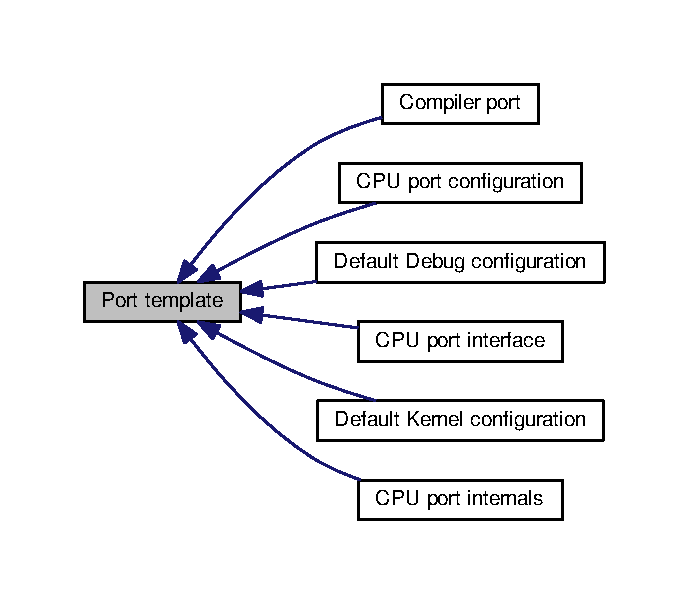
\includegraphics[width=330pt]{group__template}
\end{center}
\end{figure}
\subsubsection*{Modules}
\begin{DoxyCompactItemize}
\item 
\hyperlink{group__template__cpu__cfg}{C\-P\-U port configuration}
\begin{DoxyCompactList}\small\item\em C\-P\-U port specific configuration options. \end{DoxyCompactList}\item 
\hyperlink{group__template__cpu__intf}{C\-P\-U port interface}
\begin{DoxyCompactList}\small\item\em C\-P\-U port macros and functions. \end{DoxyCompactList}\item 
\hyperlink{group__template__cpu__impl}{C\-P\-U port internals}
\begin{DoxyCompactList}\small\item\em C\-P\-U port inner work. \end{DoxyCompactList}\item 
\hyperlink{group__template__compiler}{Compiler port}
\begin{DoxyCompactList}\small\item\em Compiler provided macros and data types. \end{DoxyCompactList}\item 
\hyperlink{group__template__dbg__cfg}{Default Debug configuration}
\begin{DoxyCompactList}\small\item\em Default Debug Configuration settings. \end{DoxyCompactList}\item 
\hyperlink{group__template__kern__cfg}{Default Kernel configuration}
\begin{DoxyCompactList}\small\item\em Default Kernel Configuration settings. \end{DoxyCompactList}\end{DoxyCompactItemize}


\subsubsection{Detailed Description}
Templates. 
\hypertarget{group__template__compiler}{\subsection{Compiler port}
\label{group__template__compiler}\index{Compiler port@{Compiler port}}
}


Compiler provided macros and data types.  


Collaboration diagram for Compiler port\-:\nopagebreak
\begin{figure}[H]
\begin{center}
\leavevmode
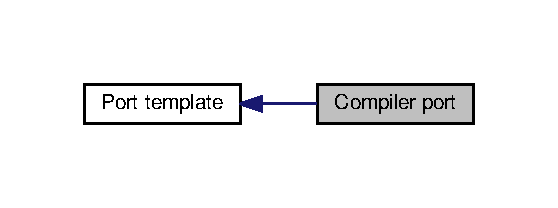
\includegraphics[width=268pt]{group__template__compiler}
\end{center}
\end{figure}
\subsubsection*{Compiler provided macros}
\label{_amgrp0f21e649732376f8320c53f1472d5e53}%
Port interface macros and port specific macros

These macros are used to ease the writing of ports. All macros prefixed with {\bfseries P\-O\-R\-T\-\_\-} are part of the port interface. \begin{DoxyCompactItemize}
\item 
\#define \hyperlink{group__template__compiler_ga87952d6e574c7f437503926e833ba345}{P\-O\-R\-T\-\_\-\-C\-\_\-\-I\-N\-L\-I\-N\-E}~inline
\begin{DoxyCompactList}\small\item\em C extension -\/ make a function inline. \end{DoxyCompactList}\item 
\#define \hyperlink{group__template__compiler_ga89152d5aab4045f552113b32920741ce}{P\-O\-R\-T\-\_\-\-C\-\_\-\-I\-N\-L\-I\-N\-E\-\_\-\-A\-L\-W\-A\-Y\-S}~inline
\begin{DoxyCompactList}\small\item\em C extension -\/ make a function inline -\/ always. \end{DoxyCompactList}\item 
\#define \hyperlink{group__template__compiler_gaf50b092bb255c796c99927cebbdb8631}{P\-O\-R\-T\-\_\-\-C\-\_\-\-N\-A\-K\-E\-D}
\begin{DoxyCompactList}\small\item\em Omit function prologue/epilogue sequences. \end{DoxyCompactList}\item 
\#define \hyperlink{group__template__compiler_ga6fe63660c6d0ccbabb032c026714863e}{P\-O\-R\-T\-\_\-\-C\-\_\-\-F\-U\-N\-C}~\char`\"{}unknown\char`\"{}
\begin{DoxyCompactList}\small\item\em Provides function name for assert macros. \end{DoxyCompactList}\item 
\#define \hyperlink{group__template__compiler_ga70c3ad4cff78229fae591d039b59f4d1}{P\-O\-R\-T\-\_\-\-C\-\_\-\-W\-E\-A\-K}
\begin{DoxyCompactList}\small\item\em Declares a weak function. \end{DoxyCompactList}\item 
\#define \hyperlink{group__template__compiler_ga4d6b8bd33e54fa5af4c5291c92dda288}{P\-O\-R\-T\-\_\-\-C\-\_\-\-A\-L\-I\-G\-N\-E\-D}(expr)
\begin{DoxyCompactList}\small\item\em This attribute specifies a minimum alignment (in bytes) for variables of the specified type. \end{DoxyCompactList}\item 
\#define \hyperlink{group__template__compiler_ga47fdf2153dba3df8c6a840829f02bd66}{P\-O\-R\-T\-\_\-\-H\-W\-R\-E\-G\-\_\-\-S\-E\-T}(reg, mask, val)
\begin{DoxyCompactList}\small\item\em A standardized way of properly setting the value of H\-W register. \end{DoxyCompactList}\end{DoxyCompactItemize}
\subsubsection*{Compiler provided data types}
\label{_amgrp0fa76376c1171116a77221ec211612f0}%
The compiler port must provide some C90 (C99) data types

The compiler port must\-:
\begin{DoxyItemize}
\item declare sets of integer types having specified widths, standard type definitions and shall define corresponding sets of macros.
\end{DoxyItemize}

Types are defined in the following categories\-:
\begin{DoxyItemize}
\item Integer types having certain exact widths
\item Fastest integer types having at least certain specified widths
\item Integer types wide enough to hold pointers to objects
\item standard type definitions
\end{DoxyItemize}

The following exact-\/width integer types are required\-:
\begin{DoxyItemize}
\item int8\-\_\-t
\item int16\-\_\-t
\item int32\-\_\-t
\item uint8\-\_\-t
\item uint16\-\_\-t
\item uint32\-\_\-t
\end{DoxyItemize}

The following fastest minimum-\/width integer types are required\-:
\begin{DoxyItemize}
\item int\-\_\-fast8\-\_\-t
\item int\-\_\-fast16\-\_\-t
\item int\-\_\-fast32\-\_\-t
\item uint\-\_\-fast8\-\_\-t
\item uint\-\_\-fast16\-\_\-t
\item uint\-\_\-fast32\-\_\-t
\end{DoxyItemize}

The following integer types capable of holding object pointers are required\-:
\begin{DoxyItemize}
\item intptr\-\_\-t
\item uintptr\-\_\-t
\end{DoxyItemize}

The following standard type definitions are required\-:
\begin{DoxyItemize}
\item N\-U\-L\-L
\item ptrdiff\-\_\-t
\item size\-\_\-t 
\end{DoxyItemize}\begin{DoxyCompactItemize}
\item 
enum \hyperlink{group__template__compiler_ga05f6c3f21a0d28271ad754637673d8fa}{bool\-Type} \{ \\*
\hyperlink{group__template__compiler_gga05f6c3f21a0d28271ad754637673d8faaa82764c3079aea4e60c80e45befbb839}{T\-R\-U\-E} = 1\-U, 
\\*
\hyperlink{group__template__compiler_gga05f6c3f21a0d28271ad754637673d8faaa1e095cc966dbecf6a0d8aad75348d1a}{F\-A\-L\-S\-E} = 0\-U
 \}
\begin{DoxyCompactList}\small\item\em Bool data type. \end{DoxyCompactList}\item 
typedef enum \hyperlink{group__template__compiler_ga05f6c3f21a0d28271ad754637673d8fa}{bool\-Type} \hyperlink{group__template__compiler_ga74fbee312f9185efb602f89d21b53404}{bool\-\_\-\-T}
\begin{DoxyCompactList}\small\item\em Bool data type. \end{DoxyCompactList}\end{DoxyCompactItemize}


\subsubsection{Detailed Description}
Compiler provided macros and data types. 

\subsubsection{Macro Definition Documentation}
\hypertarget{group__template__compiler_ga87952d6e574c7f437503926e833ba345}{\index{Compiler port@{Compiler port}!P\-O\-R\-T\-\_\-\-C\-\_\-\-I\-N\-L\-I\-N\-E@{P\-O\-R\-T\-\_\-\-C\-\_\-\-I\-N\-L\-I\-N\-E}}
\index{P\-O\-R\-T\-\_\-\-C\-\_\-\-I\-N\-L\-I\-N\-E@{P\-O\-R\-T\-\_\-\-C\-\_\-\-I\-N\-L\-I\-N\-E}!Compiler port@{Compiler port}}
\paragraph[{P\-O\-R\-T\-\_\-\-C\-\_\-\-I\-N\-L\-I\-N\-E}]{\setlength{\rightskip}{0pt plus 5cm}\#define P\-O\-R\-T\-\_\-\-C\-\_\-\-I\-N\-L\-I\-N\-E~inline}}\label{group__template__compiler_ga87952d6e574c7f437503926e833ba345}


C extension -\/ make a function inline. 

The point of making a function {\ttfamily inline} is to hint to the compiler that it is worth making some form of extra effort to call the function faster than it would otherwise -\/ generally by substituting the code of the function into its caller. As well as eliminating the need for a call and return sequence, it might allow the compiler to perform certain optimizations between the bodies of both functions. \hypertarget{group__template__compiler_ga89152d5aab4045f552113b32920741ce}{\index{Compiler port@{Compiler port}!P\-O\-R\-T\-\_\-\-C\-\_\-\-I\-N\-L\-I\-N\-E\-\_\-\-A\-L\-W\-A\-Y\-S@{P\-O\-R\-T\-\_\-\-C\-\_\-\-I\-N\-L\-I\-N\-E\-\_\-\-A\-L\-W\-A\-Y\-S}}
\index{P\-O\-R\-T\-\_\-\-C\-\_\-\-I\-N\-L\-I\-N\-E\-\_\-\-A\-L\-W\-A\-Y\-S@{P\-O\-R\-T\-\_\-\-C\-\_\-\-I\-N\-L\-I\-N\-E\-\_\-\-A\-L\-W\-A\-Y\-S}!Compiler port@{Compiler port}}
\paragraph[{P\-O\-R\-T\-\_\-\-C\-\_\-\-I\-N\-L\-I\-N\-E\-\_\-\-A\-L\-W\-A\-Y\-S}]{\setlength{\rightskip}{0pt plus 5cm}\#define P\-O\-R\-T\-\_\-\-C\-\_\-\-I\-N\-L\-I\-N\-E\-\_\-\-A\-L\-W\-A\-Y\-S~inline}}\label{group__template__compiler_ga89152d5aab4045f552113b32920741ce}


C extension -\/ make a function inline -\/ always. 

Generally, functions are not inlined unless optimization is specified. For functions declared inline, this attribute inlines the function even if no optimization level was specified. \hypertarget{group__template__compiler_gaf50b092bb255c796c99927cebbdb8631}{\index{Compiler port@{Compiler port}!P\-O\-R\-T\-\_\-\-C\-\_\-\-N\-A\-K\-E\-D@{P\-O\-R\-T\-\_\-\-C\-\_\-\-N\-A\-K\-E\-D}}
\index{P\-O\-R\-T\-\_\-\-C\-\_\-\-N\-A\-K\-E\-D@{P\-O\-R\-T\-\_\-\-C\-\_\-\-N\-A\-K\-E\-D}!Compiler port@{Compiler port}}
\paragraph[{P\-O\-R\-T\-\_\-\-C\-\_\-\-N\-A\-K\-E\-D}]{\setlength{\rightskip}{0pt plus 5cm}\#define P\-O\-R\-T\-\_\-\-C\-\_\-\-N\-A\-K\-E\-D}}\label{group__template__compiler_gaf50b092bb255c796c99927cebbdb8631}


Omit function prologue/epilogue sequences. 

This attribute will indicate that the specified function does not need prologue/epilogue sequences generated by the compiler. It is up to the programmer to provide these sequences. The only statements that can be safely included in naked functions are {\ttfamily asm} statements that do not have operands. All other statements, including declarations of local variables, {\ttfamily if} statements, and so forth, should be avoided. Naked functions should be used to implement the body of an assembly function, while allowing the compiler to construct the requisite function declaration for the assembler. \hypertarget{group__template__compiler_ga6fe63660c6d0ccbabb032c026714863e}{\index{Compiler port@{Compiler port}!P\-O\-R\-T\-\_\-\-C\-\_\-\-F\-U\-N\-C@{P\-O\-R\-T\-\_\-\-C\-\_\-\-F\-U\-N\-C}}
\index{P\-O\-R\-T\-\_\-\-C\-\_\-\-F\-U\-N\-C@{P\-O\-R\-T\-\_\-\-C\-\_\-\-F\-U\-N\-C}!Compiler port@{Compiler port}}
\paragraph[{P\-O\-R\-T\-\_\-\-C\-\_\-\-F\-U\-N\-C}]{\setlength{\rightskip}{0pt plus 5cm}\#define P\-O\-R\-T\-\_\-\-C\-\_\-\-F\-U\-N\-C~\char`\"{}unknown\char`\"{}}}\label{group__template__compiler_ga6fe63660c6d0ccbabb032c026714863e}


Provides function name for assert macros. 

\hypertarget{group__template__compiler_ga70c3ad4cff78229fae591d039b59f4d1}{\index{Compiler port@{Compiler port}!P\-O\-R\-T\-\_\-\-C\-\_\-\-W\-E\-A\-K@{P\-O\-R\-T\-\_\-\-C\-\_\-\-W\-E\-A\-K}}
\index{P\-O\-R\-T\-\_\-\-C\-\_\-\-W\-E\-A\-K@{P\-O\-R\-T\-\_\-\-C\-\_\-\-W\-E\-A\-K}!Compiler port@{Compiler port}}
\paragraph[{P\-O\-R\-T\-\_\-\-C\-\_\-\-W\-E\-A\-K}]{\setlength{\rightskip}{0pt plus 5cm}\#define P\-O\-R\-T\-\_\-\-C\-\_\-\-W\-E\-A\-K}}\label{group__template__compiler_ga70c3ad4cff78229fae591d039b59f4d1}


Declares a weak function. 

The weak attribute causes the declaration to be emitted as a weak symbol rather than a global. This is primarily useful in defining library functions that can be overridden in user code, though it can also be used with non-\/function declarations. \hypertarget{group__template__compiler_ga4d6b8bd33e54fa5af4c5291c92dda288}{\index{Compiler port@{Compiler port}!P\-O\-R\-T\-\_\-\-C\-\_\-\-A\-L\-I\-G\-N\-E\-D@{P\-O\-R\-T\-\_\-\-C\-\_\-\-A\-L\-I\-G\-N\-E\-D}}
\index{P\-O\-R\-T\-\_\-\-C\-\_\-\-A\-L\-I\-G\-N\-E\-D@{P\-O\-R\-T\-\_\-\-C\-\_\-\-A\-L\-I\-G\-N\-E\-D}!Compiler port@{Compiler port}}
\paragraph[{P\-O\-R\-T\-\_\-\-C\-\_\-\-A\-L\-I\-G\-N\-E\-D}]{\setlength{\rightskip}{0pt plus 5cm}\#define P\-O\-R\-T\-\_\-\-C\-\_\-\-A\-L\-I\-G\-N\-E\-D(
\begin{DoxyParamCaption}
\item[{}]{expr}
\end{DoxyParamCaption}
)}}\label{group__template__compiler_ga4d6b8bd33e54fa5af4c5291c92dda288}


This attribute specifies a minimum alignment (in bytes) for variables of the specified type. 

\begin{DoxyNote}{Note}
The alignment of any given struct or union type is required by the I\-S\-O C standard to be at least a perfect multiple of the lowest common multiple of the alignments of all of the members of the struct or union in question. 
\end{DoxyNote}
\hypertarget{group__template__compiler_ga47fdf2153dba3df8c6a840829f02bd66}{\index{Compiler port@{Compiler port}!P\-O\-R\-T\-\_\-\-H\-W\-R\-E\-G\-\_\-\-S\-E\-T@{P\-O\-R\-T\-\_\-\-H\-W\-R\-E\-G\-\_\-\-S\-E\-T}}
\index{P\-O\-R\-T\-\_\-\-H\-W\-R\-E\-G\-\_\-\-S\-E\-T@{P\-O\-R\-T\-\_\-\-H\-W\-R\-E\-G\-\_\-\-S\-E\-T}!Compiler port@{Compiler port}}
\paragraph[{P\-O\-R\-T\-\_\-\-H\-W\-R\-E\-G\-\_\-\-S\-E\-T}]{\setlength{\rightskip}{0pt plus 5cm}\#define P\-O\-R\-T\-\_\-\-H\-W\-R\-E\-G\-\_\-\-S\-E\-T(
\begin{DoxyParamCaption}
\item[{}]{reg, }
\item[{}]{mask, }
\item[{}]{val}
\end{DoxyParamCaption}
)}}\label{group__template__compiler_ga47fdf2153dba3df8c6a840829f02bd66}
{\bfseries Value\-:}
\begin{DoxyCode}
\textcolor{keywordflow}{do} \{                                                                        \(\backslash\)
        portReg\_T tmp;                                                          \(\backslash\)
        tmp = (reg);                                                            \(\backslash\)
        tmp &= ~(mask);                                                         \(\backslash\)
        tmp |= ((mask) & (val));                                                \(\backslash\)
        (reg) = tmp;                                                            \(\backslash\)
    \} \textcolor{keywordflow}{while} (0U)
\end{DoxyCode}


A standardized way of properly setting the value of H\-W register. 


\begin{DoxyParams}{Parameters}
{\em reg} & Register which will be written to \\
\hline
{\em mask} & The bit mask which will be applied to register and {\ttfamily val} argument \\
\hline
{\em val} & Value to be written into the register \\
\hline
\end{DoxyParams}


\subsubsection{Typedef Documentation}
\hypertarget{group__template__compiler_ga74fbee312f9185efb602f89d21b53404}{\index{Compiler port@{Compiler port}!bool\-\_\-\-T@{bool\-\_\-\-T}}
\index{bool\-\_\-\-T@{bool\-\_\-\-T}!Compiler port@{Compiler port}}
\paragraph[{bool\-\_\-\-T}]{\setlength{\rightskip}{0pt plus 5cm}typedef enum {\bf bool\-Type}  {\bf bool\-\_\-\-T}}}\label{group__template__compiler_ga74fbee312f9185efb602f89d21b53404}


Bool data type. 



\subsubsection{Enumeration Type Documentation}
\hypertarget{group__template__compiler_ga05f6c3f21a0d28271ad754637673d8fa}{\index{Compiler port@{Compiler port}!bool\-Type@{bool\-Type}}
\index{bool\-Type@{bool\-Type}!Compiler port@{Compiler port}}
\paragraph[{bool\-Type}]{\setlength{\rightskip}{0pt plus 5cm}enum {\bf bool\-Type}}}\label{group__template__compiler_ga05f6c3f21a0d28271ad754637673d8fa}


Bool data type. 

\begin{Desc}
\item[Enumerator]\par
\begin{description}
\index{T\-R\-U\-E@{T\-R\-U\-E}!Compiler port@{Compiler port}}\index{Compiler port@{Compiler port}!T\-R\-U\-E@{T\-R\-U\-E}}\item[{\em 
\hypertarget{group__template__compiler_gga05f6c3f21a0d28271ad754637673d8faaa82764c3079aea4e60c80e45befbb839}{T\-R\-U\-E}\label{group__template__compiler_gga05f6c3f21a0d28271ad754637673d8faaa82764c3079aea4e60c80e45befbb839}
}]T\-R\-U\-E. T\-R\-U\-E \index{F\-A\-L\-S\-E@{F\-A\-L\-S\-E}!Compiler port@{Compiler port}}\index{Compiler port@{Compiler port}!F\-A\-L\-S\-E@{F\-A\-L\-S\-E}}\item[{\em 
\hypertarget{group__template__compiler_gga05f6c3f21a0d28271ad754637673d8faaa1e095cc966dbecf6a0d8aad75348d1a}{F\-A\-L\-S\-E}\label{group__template__compiler_gga05f6c3f21a0d28271ad754637673d8faaa1e095cc966dbecf6a0d8aad75348d1a}
}]F\-A\-L\-S\-E. F\-A\-L\-S\-E \end{description}
\end{Desc}

\hypertarget{group__template__cpu__intf}{\subsection{C\-P\-U port interface}
\label{group__template__cpu__intf}\index{C\-P\-U port interface@{C\-P\-U port interface}}
}


C\-P\-U port macros and functions.  


Collaboration diagram for C\-P\-U port interface\-:\nopagebreak
\begin{figure}[H]
\begin{center}
\leavevmode
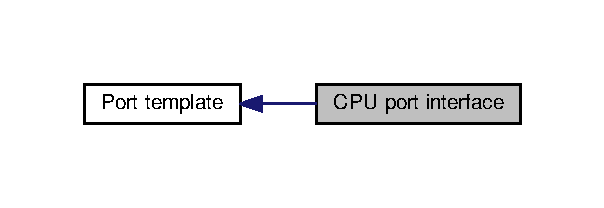
\includegraphics[width=290pt]{group__template__cpu__intf}
\end{center}
\end{figure}
\subsubsection*{Data Structures}
\begin{DoxyCompactItemize}
\item 
struct \hyperlink{structportStck}{port\-Stck}
\begin{DoxyCompactList}\small\item\em Stack structure used for stack declaration in order to force the alignment Alignment of stack structure. \end{DoxyCompactList}\item 
struct \hyperlink{structportCtx}{port\-Ctx}
\begin{DoxyCompactList}\small\item\em Port context structure. \end{DoxyCompactList}\end{DoxyCompactItemize}
\subsubsection*{Typedefs}
\begin{DoxyCompactItemize}
\item 
typedef struct \hyperlink{structportStck}{port\-Stck} \hyperlink{group__template__cpu__intf_ga13cc91970e3e05fe4210440c068d3f4a}{port\-Stck\-\_\-\-T}
\begin{DoxyCompactList}\small\item\em Stack type. \end{DoxyCompactList}\end{DoxyCompactItemize}
\subsubsection*{Variables}
\begin{DoxyCompactItemize}
\item 
port\-Reg\-\_\-\-T \hyperlink{group__template__cpu__intf_gab0ad3c664e66a9a334daa4109c14e585}{Port\-Isr\-Nesting}
\begin{DoxyCompactList}\small\item\em Variable to keep track of I\-S\-R nesting. \end{DoxyCompactList}\end{DoxyCompactItemize}
\subsubsection*{Port constants}
\begin{DoxyCompactItemize}
\item 
\#define \hyperlink{group__template__cpu__intf_ga5a629fee11006b5b0b97f7cb7176efd4}{P\-O\-R\-T\-\_\-\-D\-E\-F\-\_\-\-S\-T\-C\-K\-\_\-\-M\-I\-N\-S\-I\-Z\-E}~(sizeof(struct \hyperlink{structportCtx}{port\-Ctx}) / sizeof(port\-Reg\-\_\-\-T))
\begin{DoxyCompactList}\small\item\em This macro specifies the minimal size of the thread stack. \end{DoxyCompactList}\end{DoxyCompactItemize}
\subsubsection*{System timer constants}
\begin{DoxyCompactItemize}
\item 
\#define \hyperlink{group__template__cpu__intf_ga96e15dd16b285b0feb6e225b0834ad10}{P\-O\-R\-T\-\_\-\-D\-E\-F\-\_\-\-S\-Y\-S\-T\-M\-R\-\_\-\-W\-A\-K\-E\-U\-P\-\_\-\-T\-H\-\_\-\-V\-A\-L}~600u
\begin{DoxyCompactList}\small\item\em Threshold system timer value for new tick. \end{DoxyCompactList}\end{DoxyCompactItemize}
\subsubsection*{Kernel threads port dependent settings}
\label{_amgrp0e6f87e4f5cc0437b98e154b3e410859}%
Kernel uses several threads for system management. This section defines port dependent settings for the threads. \begin{DoxyCompactItemize}
\item 
\#define \hyperlink{group__template__cpu__intf_gabaa296d76c28043a60531ad8ed81504b}{P\-O\-R\-T\-\_\-\-D\-E\-F\-\_\-\-K\-V\-T\-M\-R\-\_\-\-S\-T\-C\-K\-\_\-\-S\-I\-Z\-E}~40u
\begin{DoxyCompactList}\small\item\em Kernel Virtual Timer Thread stack size. \end{DoxyCompactList}\item 
\#define \hyperlink{group__template__cpu__intf_ga31d47ffb78c3755575e66821b3a72a62}{P\-O\-R\-T\-\_\-\-D\-E\-F\-\_\-\-K\-I\-D\-L\-E\-\_\-\-S\-T\-C\-K\-\_\-\-S\-I\-Z\-E}~40u
\begin{DoxyCompactList}\small\item\em Kernel Idle Thread stack size. \end{DoxyCompactList}\end{DoxyCompactItemize}
\subsubsection*{Interrupt management}
\label{_amgrp0762f598cbb5b37886374004ead985d4}%
P\-O\-R\-T\-\_\-\-I\-S\-R\-\_\-... macros are used by es\-Kern\-Isr\-Enter() and es\-Kern\-Isr\-Exit() functions. They are used to keep the current level of I\-S\-R nesting. Scheduler should be invoked only from the last I\-S\-R that is executing. \begin{DoxyCompactItemize}
\item 
\#define \hyperlink{group__template__cpu__intf_gaccad9298c874b29753b318d4f900cb75}{P\-O\-R\-T\-\_\-\-I\-S\-R\-\_\-\-E\-N\-T\-E\-R}()
\begin{DoxyCompactList}\small\item\em Enter I\-S\-R. Increment Port\-Isr\-Nesting variable to keep track of I\-S\-R nesting. \end{DoxyCompactList}\item 
\#define \hyperlink{group__template__cpu__intf_ga267c312d7321e9361b454f4274bbc087}{P\-O\-R\-T\-\_\-\-I\-S\-R\-\_\-\-E\-X\-I\-T}()
\begin{DoxyCompactList}\small\item\em Exit I\-S\-R. Decrement Port\-Isr\-Nesting variable to keep track of I\-S\-R nesting. \end{DoxyCompactList}\item 
\#define \hyperlink{group__template__cpu__intf_ga6c0ea20c8e1f6b9751f51916da8e2aee}{P\-O\-R\-T\-\_\-\-I\-S\-R\-\_\-\-I\-S\-\_\-\-L\-A\-S\-T}()~(0u == Port\-Isr\-Nesting ? T\-R\-U\-E \-: F\-A\-L\-S\-E)
\begin{DoxyCompactList}\small\item\em If isr\-Nesting variable is zero then the last I\-S\-R is executing and scheduler should be invoked. \end{DoxyCompactList}\end{DoxyCompactItemize}
\subsubsection*{Dispatcher context switching}
\begin{DoxyCompactItemize}
\item 
void $\ast$ \hyperlink{group__template__cpu__intf_gaa097ec2ead487892969bcd2806539822}{port\-Ctx\-Init} (void $\ast$stck, size\-\_\-t stck\-Size, void($\ast$fn)(void $\ast$), void $\ast$arg)
\begin{DoxyCompactList}\small\item\em Initialize the thread context. \end{DoxyCompactList}\item 
\#define \hyperlink{group__template__cpu__intf_ga80d15a56d61c9d4e786e52006ff4ac43}{P\-O\-R\-T\-\_\-\-C\-T\-X\-\_\-\-I\-N\-I\-T}(stck, stack\-Size, thread, arg)
\begin{DoxyCompactList}\small\item\em Initialize the thread context. \end{DoxyCompactList}\item 
\#define \hyperlink{group__template__cpu__intf_ga50a3b72a7f2065922811f0d6dedda01a}{P\-O\-R\-T\-\_\-\-C\-T\-X\-\_\-\-S\-W}()
\begin{DoxyCompactList}\small\item\em Do the context switch -\/ invoked from A\-P\-I level. \end{DoxyCompactList}\item 
\#define \hyperlink{group__template__cpu__intf_ga20bba8f9c5a2f38fd7c63b9d2320e511}{P\-O\-R\-T\-\_\-\-C\-T\-X\-\_\-\-S\-W\-\_\-\-I\-S\-R}()
\begin{DoxyCompactList}\small\item\em Do the context switch -\/ invoked from I\-S\-R level. \end{DoxyCompactList}\item 
\#define \hyperlink{group__template__cpu__intf_ga58056289ebeda87723f99f5431c6239e}{P\-O\-R\-T\-\_\-\-C\-T\-X\-\_\-\-S\-W\-\_\-\-S\-T\-A\-R\-T}()
\begin{DoxyCompactList}\small\item\em Start the first thread. \end{DoxyCompactList}\end{DoxyCompactItemize}
\subsubsection*{General port macros}
\begin{DoxyCompactItemize}
\item 
\#define \hyperlink{group__template__cpu__intf_gabf0ea7d36355a7133ee9e9f8abafa6ff}{P\-O\-R\-T\-\_\-\-K\-C\-O\-R\-E\-\_\-\-I\-N\-I\-T\-\_\-\-E\-A\-R\-L\-Y}()
\begin{DoxyCompactList}\small\item\em Early port initialization. \end{DoxyCompactList}\item 
\#define \hyperlink{group__template__cpu__intf_ga682a913f5439544d4f0ee14ae68507fd}{P\-O\-R\-T\-\_\-\-K\-C\-O\-R\-E\-\_\-\-I\-N\-I\-T}()
\begin{DoxyCompactList}\small\item\em Port initialization. \end{DoxyCompactList}\item 
\#define \hyperlink{group__template__cpu__intf_ga5c133105168261f1744abf3c5917a515}{P\-O\-R\-T\-\_\-\-K\-C\-O\-R\-E\-\_\-\-I\-N\-I\-T\-\_\-\-L\-A\-T\-E}()
\begin{DoxyCompactList}\small\item\em Late port initialization. \end{DoxyCompactList}\item 
\#define \hyperlink{group__template__cpu__intf_gac386e206a8b5225c9aa56be88b625837}{P\-O\-R\-T\-\_\-\-K\-C\-O\-R\-E\-\_\-\-T\-E\-R\-M}()
\begin{DoxyCompactList}\small\item\em Terminate port. \end{DoxyCompactList}\item 
\#define \hyperlink{group__template__cpu__intf_gacb3a46e89d327fbaf5c122fe23877b24}{P\-O\-R\-T\-\_\-\-S\-T\-C\-K\-\_\-\-S\-I\-Z\-E}(size)~(size + \hyperlink{group__template__cpu__intf_ga5a629fee11006b5b0b97f7cb7176efd4}{P\-O\-R\-T\-\_\-\-D\-E\-F\-\_\-\-S\-T\-C\-K\-\_\-\-M\-I\-N\-S\-I\-Z\-E})
\begin{DoxyCompactList}\small\item\em Calculate the stack size. \end{DoxyCompactList}\item 
\#define \hyperlink{group__template__cpu__intf_gad699a79233d442ae90a69c113e314542}{P\-O\-R\-T\-\_\-\-C\-R\-I\-T\-I\-C\-A\-L\-\_\-\-E\-X\-I\-T\-\_\-\-S\-L\-E\-E\-P}()~port\-Int\-Set\-Sleep\-Enter\-\_\-(int\-Status\-\_\-)
\begin{DoxyCompactList}\small\item\em Exit critical section and enter sleep state. \end{DoxyCompactList}\end{DoxyCompactItemize}


\subsubsection{Detailed Description}
C\-P\-U port macros and functions. Since this header file is included with the A\-P\-I of the kernel a few naming conventions are defined in order to avoid name clashing with the names of objects from libraries included by application code.

\begin{DoxyParagraph}{1) Macro naming conventions}
For macro naming try to follow these rules\-:
\begin{DoxyItemize}
\item All standard P\-O\-R\-T A\-P\-I macro names are prefixed with\-: {\bfseries {\ttfamily P\-O\-R\-T\-\_\-}.} 
\item All other macros which are specific to the port used are prefixed with\-: {\bfseries {\ttfamily C\-P\-U\-\_\-}.} 
\end{DoxyItemize}
\end{DoxyParagraph}
\begin{DoxyParagraph}{2) Type declaration naming conventions}
For type declaration naming try to follow these rules\-:
\begin{DoxyItemize}
\item All type declaration names are prefixed with\-: {\bfseries {\ttfamily port}.} 
\end{DoxyItemize}
\end{DoxyParagraph}
\begin{DoxyParagraph}{3) Global variable naming conventions}
For global variable naming try to follow these rules\-:
\begin{DoxyItemize}
\item All global variable names are prefixed with\-: {\bfseries {\ttfamily Port}.} 
\end{DoxyItemize}
\end{DoxyParagraph}
\begin{DoxyParagraph}{4) Function naming conventions}
For functions naming try to follow these rules\-:
\begin{DoxyItemize}
\item All standard P\-O\-R\-T A\-P\-I function names are prefixed with\-: {\bfseries {\ttfamily port}}.
\item All other functions which are specific to the port used are prefixed with\-: {\bfseries {\ttfamily cpu}}
\item All inline functions are additionally postfixed with\-: {\bfseries {\ttfamily \-\_\-} }(underscore).
\item The {\ttfamily exception} to above two rules are the names of functions used for Interrupt Service Routines. They can have any name required by the port. 
\end{DoxyItemize}
\end{DoxyParagraph}


\subsubsection{Macro Definition Documentation}
\hypertarget{group__template__cpu__intf_ga5a629fee11006b5b0b97f7cb7176efd4}{\index{C\-P\-U port interface@{C\-P\-U port interface}!P\-O\-R\-T\-\_\-\-D\-E\-F\-\_\-\-S\-T\-C\-K\-\_\-\-M\-I\-N\-S\-I\-Z\-E@{P\-O\-R\-T\-\_\-\-D\-E\-F\-\_\-\-S\-T\-C\-K\-\_\-\-M\-I\-N\-S\-I\-Z\-E}}
\index{P\-O\-R\-T\-\_\-\-D\-E\-F\-\_\-\-S\-T\-C\-K\-\_\-\-M\-I\-N\-S\-I\-Z\-E@{P\-O\-R\-T\-\_\-\-D\-E\-F\-\_\-\-S\-T\-C\-K\-\_\-\-M\-I\-N\-S\-I\-Z\-E}!CPU port interface@{C\-P\-U port interface}}
\paragraph[{P\-O\-R\-T\-\_\-\-D\-E\-F\-\_\-\-S\-T\-C\-K\-\_\-\-M\-I\-N\-S\-I\-Z\-E}]{\setlength{\rightskip}{0pt plus 5cm}\#define P\-O\-R\-T\-\_\-\-D\-E\-F\-\_\-\-S\-T\-C\-K\-\_\-\-M\-I\-N\-S\-I\-Z\-E~(sizeof(struct {\bf port\-Ctx}) / sizeof(port\-Reg\-\_\-\-T))}}\label{group__template__cpu__intf_ga5a629fee11006b5b0b97f7cb7176efd4}


This macro specifies the minimal size of the thread stack. 

Generally minimal stack size is equal to the size of context structure \hypertarget{group__template__cpu__intf_ga96e15dd16b285b0feb6e225b0834ad10}{\index{C\-P\-U port interface@{C\-P\-U port interface}!P\-O\-R\-T\-\_\-\-D\-E\-F\-\_\-\-S\-Y\-S\-T\-M\-R\-\_\-\-W\-A\-K\-E\-U\-P\-\_\-\-T\-H\-\_\-\-V\-A\-L@{P\-O\-R\-T\-\_\-\-D\-E\-F\-\_\-\-S\-Y\-S\-T\-M\-R\-\_\-\-W\-A\-K\-E\-U\-P\-\_\-\-T\-H\-\_\-\-V\-A\-L}}
\index{P\-O\-R\-T\-\_\-\-D\-E\-F\-\_\-\-S\-Y\-S\-T\-M\-R\-\_\-\-W\-A\-K\-E\-U\-P\-\_\-\-T\-H\-\_\-\-V\-A\-L@{P\-O\-R\-T\-\_\-\-D\-E\-F\-\_\-\-S\-Y\-S\-T\-M\-R\-\_\-\-W\-A\-K\-E\-U\-P\-\_\-\-T\-H\-\_\-\-V\-A\-L}!CPU port interface@{C\-P\-U port interface}}
\paragraph[{P\-O\-R\-T\-\_\-\-D\-E\-F\-\_\-\-S\-Y\-S\-T\-M\-R\-\_\-\-W\-A\-K\-E\-U\-P\-\_\-\-T\-H\-\_\-\-V\-A\-L}]{\setlength{\rightskip}{0pt plus 5cm}\#define P\-O\-R\-T\-\_\-\-D\-E\-F\-\_\-\-S\-Y\-S\-T\-M\-R\-\_\-\-W\-A\-K\-E\-U\-P\-\_\-\-T\-H\-\_\-\-V\-A\-L~600u}}\label{group__template__cpu__intf_ga96e15dd16b285b0feb6e225b0834ad10}


Threshold system timer value for new tick. 

\hypertarget{group__template__cpu__intf_gabaa296d76c28043a60531ad8ed81504b}{\index{C\-P\-U port interface@{C\-P\-U port interface}!P\-O\-R\-T\-\_\-\-D\-E\-F\-\_\-\-K\-V\-T\-M\-R\-\_\-\-S\-T\-C\-K\-\_\-\-S\-I\-Z\-E@{P\-O\-R\-T\-\_\-\-D\-E\-F\-\_\-\-K\-V\-T\-M\-R\-\_\-\-S\-T\-C\-K\-\_\-\-S\-I\-Z\-E}}
\index{P\-O\-R\-T\-\_\-\-D\-E\-F\-\_\-\-K\-V\-T\-M\-R\-\_\-\-S\-T\-C\-K\-\_\-\-S\-I\-Z\-E@{P\-O\-R\-T\-\_\-\-D\-E\-F\-\_\-\-K\-V\-T\-M\-R\-\_\-\-S\-T\-C\-K\-\_\-\-S\-I\-Z\-E}!CPU port interface@{C\-P\-U port interface}}
\paragraph[{P\-O\-R\-T\-\_\-\-D\-E\-F\-\_\-\-K\-V\-T\-M\-R\-\_\-\-S\-T\-C\-K\-\_\-\-S\-I\-Z\-E}]{\setlength{\rightskip}{0pt plus 5cm}\#define P\-O\-R\-T\-\_\-\-D\-E\-F\-\_\-\-K\-V\-T\-M\-R\-\_\-\-S\-T\-C\-K\-\_\-\-S\-I\-Z\-E~40u}}\label{group__template__cpu__intf_gabaa296d76c28043a60531ad8ed81504b}


Kernel Virtual Timer Thread stack size. 

\begin{DoxyRefDesc}{Todo}
\item[\hyperlink{todo__todo000001}{Todo}]This value needs tweaking \end{DoxyRefDesc}
\hypertarget{group__template__cpu__intf_ga31d47ffb78c3755575e66821b3a72a62}{\index{C\-P\-U port interface@{C\-P\-U port interface}!P\-O\-R\-T\-\_\-\-D\-E\-F\-\_\-\-K\-I\-D\-L\-E\-\_\-\-S\-T\-C\-K\-\_\-\-S\-I\-Z\-E@{P\-O\-R\-T\-\_\-\-D\-E\-F\-\_\-\-K\-I\-D\-L\-E\-\_\-\-S\-T\-C\-K\-\_\-\-S\-I\-Z\-E}}
\index{P\-O\-R\-T\-\_\-\-D\-E\-F\-\_\-\-K\-I\-D\-L\-E\-\_\-\-S\-T\-C\-K\-\_\-\-S\-I\-Z\-E@{P\-O\-R\-T\-\_\-\-D\-E\-F\-\_\-\-K\-I\-D\-L\-E\-\_\-\-S\-T\-C\-K\-\_\-\-S\-I\-Z\-E}!CPU port interface@{C\-P\-U port interface}}
\paragraph[{P\-O\-R\-T\-\_\-\-D\-E\-F\-\_\-\-K\-I\-D\-L\-E\-\_\-\-S\-T\-C\-K\-\_\-\-S\-I\-Z\-E}]{\setlength{\rightskip}{0pt plus 5cm}\#define P\-O\-R\-T\-\_\-\-D\-E\-F\-\_\-\-K\-I\-D\-L\-E\-\_\-\-S\-T\-C\-K\-\_\-\-S\-I\-Z\-E~40u}}\label{group__template__cpu__intf_ga31d47ffb78c3755575e66821b3a72a62}


Kernel Idle Thread stack size. 

\begin{DoxyRefDesc}{Todo}
\item[\hyperlink{todo__todo000002}{Todo}]This value needs tweaking \end{DoxyRefDesc}
\hypertarget{group__template__cpu__intf_gaccad9298c874b29753b318d4f900cb75}{\index{C\-P\-U port interface@{C\-P\-U port interface}!P\-O\-R\-T\-\_\-\-I\-S\-R\-\_\-\-E\-N\-T\-E\-R@{P\-O\-R\-T\-\_\-\-I\-S\-R\-\_\-\-E\-N\-T\-E\-R}}
\index{P\-O\-R\-T\-\_\-\-I\-S\-R\-\_\-\-E\-N\-T\-E\-R@{P\-O\-R\-T\-\_\-\-I\-S\-R\-\_\-\-E\-N\-T\-E\-R}!CPU port interface@{C\-P\-U port interface}}
\paragraph[{P\-O\-R\-T\-\_\-\-I\-S\-R\-\_\-\-E\-N\-T\-E\-R}]{\setlength{\rightskip}{0pt plus 5cm}\#define P\-O\-R\-T\-\_\-\-I\-S\-R\-\_\-\-E\-N\-T\-E\-R(
\begin{DoxyParamCaption}
{}
\end{DoxyParamCaption}
)}}\label{group__template__cpu__intf_gaccad9298c874b29753b318d4f900cb75}
{\bfseries Value\-:}
\begin{DoxyCode}
\textcolor{keywordflow}{do} \{                                                                        \hyperlink{group__template__cpu__intf_gab0ad3c664e66a9a334daa4109c14e585}{\(\backslash\)}
\hyperlink{group__template__cpu__intf_gab0ad3c664e66a9a334daa4109c14e585}{        PortIsrNesting}++;                                                       
      \hyperlink{group__kern__general_gac0d578bcd4a10b2c8e5fc90f0b86ccec}{\(\backslash\)}
\hyperlink{group__kern__general_gac0d578bcd4a10b2c8e5fc90f0b86ccec}{        esKernIsrEnterI}();                                                      \(\backslash\)
    \} \textcolor{keywordflow}{while} (0u)
\end{DoxyCode}


Enter I\-S\-R. Increment Port\-Isr\-Nesting variable to keep track of I\-S\-R nesting. 

Variable Port\-Isr\-Nesting is needed only if the port does not support any other method of detecting when the last I\-S\-R is executing. \hypertarget{group__template__cpu__intf_ga267c312d7321e9361b454f4274bbc087}{\index{C\-P\-U port interface@{C\-P\-U port interface}!P\-O\-R\-T\-\_\-\-I\-S\-R\-\_\-\-E\-X\-I\-T@{P\-O\-R\-T\-\_\-\-I\-S\-R\-\_\-\-E\-X\-I\-T}}
\index{P\-O\-R\-T\-\_\-\-I\-S\-R\-\_\-\-E\-X\-I\-T@{P\-O\-R\-T\-\_\-\-I\-S\-R\-\_\-\-E\-X\-I\-T}!CPU port interface@{C\-P\-U port interface}}
\paragraph[{P\-O\-R\-T\-\_\-\-I\-S\-R\-\_\-\-E\-X\-I\-T}]{\setlength{\rightskip}{0pt plus 5cm}\#define P\-O\-R\-T\-\_\-\-I\-S\-R\-\_\-\-E\-X\-I\-T(
\begin{DoxyParamCaption}
{}
\end{DoxyParamCaption}
)}}\label{group__template__cpu__intf_ga267c312d7321e9361b454f4274bbc087}
{\bfseries Value\-:}
\begin{DoxyCode}
\textcolor{keywordflow}{do} \{                                                                        \hyperlink{group__template__cpu__intf_gab0ad3c664e66a9a334daa4109c14e585}{\(\backslash\)}
\hyperlink{group__template__cpu__intf_gab0ad3c664e66a9a334daa4109c14e585}{        PortIsrNesting}--;                                                       
      \hyperlink{group__kern__general_gaa6347925fff1684b5425dd2857c27129}{\(\backslash\)}
\hyperlink{group__kern__general_gaa6347925fff1684b5425dd2857c27129}{        esKernIsrExitI}();                                                       \(\backslash\)
    \} \textcolor{keywordflow}{while} (0u)
\end{DoxyCode}


Exit I\-S\-R. Decrement Port\-Isr\-Nesting variable to keep track of I\-S\-R nesting. 

Variable Port\-Isr\-Nesting is needed only if the port does not support any other method of detecting when the last I\-S\-R is executing. \hypertarget{group__template__cpu__intf_ga6c0ea20c8e1f6b9751f51916da8e2aee}{\index{C\-P\-U port interface@{C\-P\-U port interface}!P\-O\-R\-T\-\_\-\-I\-S\-R\-\_\-\-I\-S\-\_\-\-L\-A\-S\-T@{P\-O\-R\-T\-\_\-\-I\-S\-R\-\_\-\-I\-S\-\_\-\-L\-A\-S\-T}}
\index{P\-O\-R\-T\-\_\-\-I\-S\-R\-\_\-\-I\-S\-\_\-\-L\-A\-S\-T@{P\-O\-R\-T\-\_\-\-I\-S\-R\-\_\-\-I\-S\-\_\-\-L\-A\-S\-T}!CPU port interface@{C\-P\-U port interface}}
\paragraph[{P\-O\-R\-T\-\_\-\-I\-S\-R\-\_\-\-I\-S\-\_\-\-L\-A\-S\-T}]{\setlength{\rightskip}{0pt plus 5cm}\#define P\-O\-R\-T\-\_\-\-I\-S\-R\-\_\-\-I\-S\-\_\-\-L\-A\-S\-T(
\begin{DoxyParamCaption}
{}
\end{DoxyParamCaption}
)~(0u == Port\-Isr\-Nesting ? T\-R\-U\-E \-: F\-A\-L\-S\-E)}}\label{group__template__cpu__intf_ga6c0ea20c8e1f6b9751f51916da8e2aee}


If isr\-Nesting variable is zero then the last I\-S\-R is executing and scheduler should be invoked. 

\begin{DoxyReturn}{Returns}
Is the currently executed I\-S\-R the last one? 
\end{DoxyReturn}

\begin{DoxyRetVals}{Return values}
{\em T\-R\-U\-E} & -\/ this is last I\-S\-R \\
\hline
{\em F\-A\-L\-S\-E} & -\/ this is not the last I\-S\-R \\
\hline
\end{DoxyRetVals}
\hypertarget{group__template__cpu__intf_ga80d15a56d61c9d4e786e52006ff4ac43}{\index{C\-P\-U port interface@{C\-P\-U port interface}!P\-O\-R\-T\-\_\-\-C\-T\-X\-\_\-\-I\-N\-I\-T@{P\-O\-R\-T\-\_\-\-C\-T\-X\-\_\-\-I\-N\-I\-T}}
\index{P\-O\-R\-T\-\_\-\-C\-T\-X\-\_\-\-I\-N\-I\-T@{P\-O\-R\-T\-\_\-\-C\-T\-X\-\_\-\-I\-N\-I\-T}!CPU port interface@{C\-P\-U port interface}}
\paragraph[{P\-O\-R\-T\-\_\-\-C\-T\-X\-\_\-\-I\-N\-I\-T}]{\setlength{\rightskip}{0pt plus 5cm}\#define P\-O\-R\-T\-\_\-\-C\-T\-X\-\_\-\-I\-N\-I\-T(
\begin{DoxyParamCaption}
\item[{}]{stck, }
\item[{}]{stack\-Size, }
\item[{}]{thread, }
\item[{}]{arg}
\end{DoxyParamCaption}
)}}\label{group__template__cpu__intf_ga80d15a56d61c9d4e786e52006ff4ac43}


Initialize the thread context. 


\begin{DoxyParams}[1]{Parameters}
\mbox{\tt in,out}  & {\em stck} & Pointer to the allocated thread stack. The pointer points to the beginning of the memory as defined per C language. It's up to port function to adjust the pointer according to the stack type\-: full descending or full ascending one. \\
\hline
 & {\em stack\-Size} & The size of allocated stack in bytes. \\
\hline
\mbox{\tt in}  & {\em thread} & Pointer to the thread function. \\
\hline
\mbox{\tt in}  & {\em arg} & Argument that will be passed to thread function at the starting of execution. \\
\hline
\end{DoxyParams}
\begin{DoxyReturn}{Returns}
The new top of stack after thread context initialization. 
\end{DoxyReturn}
\hypertarget{group__template__cpu__intf_ga50a3b72a7f2065922811f0d6dedda01a}{\index{C\-P\-U port interface@{C\-P\-U port interface}!P\-O\-R\-T\-\_\-\-C\-T\-X\-\_\-\-S\-W@{P\-O\-R\-T\-\_\-\-C\-T\-X\-\_\-\-S\-W}}
\index{P\-O\-R\-T\-\_\-\-C\-T\-X\-\_\-\-S\-W@{P\-O\-R\-T\-\_\-\-C\-T\-X\-\_\-\-S\-W}!CPU port interface@{C\-P\-U port interface}}
\paragraph[{P\-O\-R\-T\-\_\-\-C\-T\-X\-\_\-\-S\-W}]{\setlength{\rightskip}{0pt plus 5cm}\#define P\-O\-R\-T\-\_\-\-C\-T\-X\-\_\-\-S\-W(
\begin{DoxyParamCaption}
{}
\end{DoxyParamCaption}
)}}\label{group__template__cpu__intf_ga50a3b72a7f2065922811f0d6dedda01a}


Do the context switch -\/ invoked from A\-P\-I level. 

\hypertarget{group__template__cpu__intf_ga20bba8f9c5a2f38fd7c63b9d2320e511}{\index{C\-P\-U port interface@{C\-P\-U port interface}!P\-O\-R\-T\-\_\-\-C\-T\-X\-\_\-\-S\-W\-\_\-\-I\-S\-R@{P\-O\-R\-T\-\_\-\-C\-T\-X\-\_\-\-S\-W\-\_\-\-I\-S\-R}}
\index{P\-O\-R\-T\-\_\-\-C\-T\-X\-\_\-\-S\-W\-\_\-\-I\-S\-R@{P\-O\-R\-T\-\_\-\-C\-T\-X\-\_\-\-S\-W\-\_\-\-I\-S\-R}!CPU port interface@{C\-P\-U port interface}}
\paragraph[{P\-O\-R\-T\-\_\-\-C\-T\-X\-\_\-\-S\-W\-\_\-\-I\-S\-R}]{\setlength{\rightskip}{0pt plus 5cm}\#define P\-O\-R\-T\-\_\-\-C\-T\-X\-\_\-\-S\-W\-\_\-\-I\-S\-R(
\begin{DoxyParamCaption}
{}
\end{DoxyParamCaption}
)}}\label{group__template__cpu__intf_ga20bba8f9c5a2f38fd7c63b9d2320e511}


Do the context switch -\/ invoked from I\-S\-R level. 

\hypertarget{group__template__cpu__intf_ga58056289ebeda87723f99f5431c6239e}{\index{C\-P\-U port interface@{C\-P\-U port interface}!P\-O\-R\-T\-\_\-\-C\-T\-X\-\_\-\-S\-W\-\_\-\-S\-T\-A\-R\-T@{P\-O\-R\-T\-\_\-\-C\-T\-X\-\_\-\-S\-W\-\_\-\-S\-T\-A\-R\-T}}
\index{P\-O\-R\-T\-\_\-\-C\-T\-X\-\_\-\-S\-W\-\_\-\-S\-T\-A\-R\-T@{P\-O\-R\-T\-\_\-\-C\-T\-X\-\_\-\-S\-W\-\_\-\-S\-T\-A\-R\-T}!CPU port interface@{C\-P\-U port interface}}
\paragraph[{P\-O\-R\-T\-\_\-\-C\-T\-X\-\_\-\-S\-W\-\_\-\-S\-T\-A\-R\-T}]{\setlength{\rightskip}{0pt plus 5cm}\#define P\-O\-R\-T\-\_\-\-C\-T\-X\-\_\-\-S\-W\-\_\-\-S\-T\-A\-R\-T(
\begin{DoxyParamCaption}
{}
\end{DoxyParamCaption}
)}}\label{group__template__cpu__intf_ga58056289ebeda87723f99f5431c6239e}


Start the first thread. 

\hypertarget{group__template__cpu__intf_gabf0ea7d36355a7133ee9e9f8abafa6ff}{\index{C\-P\-U port interface@{C\-P\-U port interface}!P\-O\-R\-T\-\_\-\-K\-C\-O\-R\-E\-\_\-\-I\-N\-I\-T\-\_\-\-E\-A\-R\-L\-Y@{P\-O\-R\-T\-\_\-\-K\-C\-O\-R\-E\-\_\-\-I\-N\-I\-T\-\_\-\-E\-A\-R\-L\-Y}}
\index{P\-O\-R\-T\-\_\-\-K\-C\-O\-R\-E\-\_\-\-I\-N\-I\-T\-\_\-\-E\-A\-R\-L\-Y@{P\-O\-R\-T\-\_\-\-K\-C\-O\-R\-E\-\_\-\-I\-N\-I\-T\-\_\-\-E\-A\-R\-L\-Y}!CPU port interface@{C\-P\-U port interface}}
\paragraph[{P\-O\-R\-T\-\_\-\-K\-C\-O\-R\-E\-\_\-\-I\-N\-I\-T\-\_\-\-E\-A\-R\-L\-Y}]{\setlength{\rightskip}{0pt plus 5cm}\#define P\-O\-R\-T\-\_\-\-K\-C\-O\-R\-E\-\_\-\-I\-N\-I\-T\-\_\-\-E\-A\-R\-L\-Y(
\begin{DoxyParamCaption}
{}
\end{DoxyParamCaption}
)}}\label{group__template__cpu__intf_gabf0ea7d36355a7133ee9e9f8abafa6ff}


Early port initialization. 

This macro will be called at early initialization stage from \hyperlink{group__kern__general_ga9e9ff699d62d6035cd51121bb3140704}{es\-Kern\-Init()} function. It is called before any kernel data initialization. Usually this macro would be used to setup memory space, fill the memory with debug value or something similar. \hypertarget{group__template__cpu__intf_ga682a913f5439544d4f0ee14ae68507fd}{\index{C\-P\-U port interface@{C\-P\-U port interface}!P\-O\-R\-T\-\_\-\-K\-C\-O\-R\-E\-\_\-\-I\-N\-I\-T@{P\-O\-R\-T\-\_\-\-K\-C\-O\-R\-E\-\_\-\-I\-N\-I\-T}}
\index{P\-O\-R\-T\-\_\-\-K\-C\-O\-R\-E\-\_\-\-I\-N\-I\-T@{P\-O\-R\-T\-\_\-\-K\-C\-O\-R\-E\-\_\-\-I\-N\-I\-T}!CPU port interface@{C\-P\-U port interface}}
\paragraph[{P\-O\-R\-T\-\_\-\-K\-C\-O\-R\-E\-\_\-\-I\-N\-I\-T}]{\setlength{\rightskip}{0pt plus 5cm}\#define P\-O\-R\-T\-\_\-\-K\-C\-O\-R\-E\-\_\-\-I\-N\-I\-T(
\begin{DoxyParamCaption}
{}
\end{DoxyParamCaption}
)}}\label{group__template__cpu__intf_ga682a913f5439544d4f0ee14ae68507fd}


Port initialization. 

This macro will be called after kernel data structure initialization from \hyperlink{group__kern__general_ga9e9ff699d62d6035cd51121bb3140704}{es\-Kern\-Init()} function. \hypertarget{group__template__cpu__intf_ga5c133105168261f1744abf3c5917a515}{\index{C\-P\-U port interface@{C\-P\-U port interface}!P\-O\-R\-T\-\_\-\-K\-C\-O\-R\-E\-\_\-\-I\-N\-I\-T\-\_\-\-L\-A\-T\-E@{P\-O\-R\-T\-\_\-\-K\-C\-O\-R\-E\-\_\-\-I\-N\-I\-T\-\_\-\-L\-A\-T\-E}}
\index{P\-O\-R\-T\-\_\-\-K\-C\-O\-R\-E\-\_\-\-I\-N\-I\-T\-\_\-\-L\-A\-T\-E@{P\-O\-R\-T\-\_\-\-K\-C\-O\-R\-E\-\_\-\-I\-N\-I\-T\-\_\-\-L\-A\-T\-E}!CPU port interface@{C\-P\-U port interface}}
\paragraph[{P\-O\-R\-T\-\_\-\-K\-C\-O\-R\-E\-\_\-\-I\-N\-I\-T\-\_\-\-L\-A\-T\-E}]{\setlength{\rightskip}{0pt plus 5cm}\#define P\-O\-R\-T\-\_\-\-K\-C\-O\-R\-E\-\_\-\-I\-N\-I\-T\-\_\-\-L\-A\-T\-E(
\begin{DoxyParamCaption}
{}
\end{DoxyParamCaption}
)}}\label{group__template__cpu__intf_ga5c133105168261f1744abf3c5917a515}


Late port initialization. 

This macro will be called just a moment before the multitasking is started. The macro is called from \hyperlink{group__kern__general_ga0e7a0a6b9c02df58de0f98de0229a09d}{es\-Kern\-Start()} function. \hypertarget{group__template__cpu__intf_gac386e206a8b5225c9aa56be88b625837}{\index{C\-P\-U port interface@{C\-P\-U port interface}!P\-O\-R\-T\-\_\-\-K\-C\-O\-R\-E\-\_\-\-T\-E\-R\-M@{P\-O\-R\-T\-\_\-\-K\-C\-O\-R\-E\-\_\-\-T\-E\-R\-M}}
\index{P\-O\-R\-T\-\_\-\-K\-C\-O\-R\-E\-\_\-\-T\-E\-R\-M@{P\-O\-R\-T\-\_\-\-K\-C\-O\-R\-E\-\_\-\-T\-E\-R\-M}!CPU port interface@{C\-P\-U port interface}}
\paragraph[{P\-O\-R\-T\-\_\-\-K\-C\-O\-R\-E\-\_\-\-T\-E\-R\-M}]{\setlength{\rightskip}{0pt plus 5cm}\#define P\-O\-R\-T\-\_\-\-K\-C\-O\-R\-E\-\_\-\-T\-E\-R\-M(
\begin{DoxyParamCaption}
{}
\end{DoxyParamCaption}
)}}\label{group__template__cpu__intf_gac386e206a8b5225c9aa56be88b625837}


Terminate port. 

This macro will be called when there is a need to stop any further execution (example\-: an error occurred and C\-P\-U needs to stop). \hypertarget{group__template__cpu__intf_gacb3a46e89d327fbaf5c122fe23877b24}{\index{C\-P\-U port interface@{C\-P\-U port interface}!P\-O\-R\-T\-\_\-\-S\-T\-C\-K\-\_\-\-S\-I\-Z\-E@{P\-O\-R\-T\-\_\-\-S\-T\-C\-K\-\_\-\-S\-I\-Z\-E}}
\index{P\-O\-R\-T\-\_\-\-S\-T\-C\-K\-\_\-\-S\-I\-Z\-E@{P\-O\-R\-T\-\_\-\-S\-T\-C\-K\-\_\-\-S\-I\-Z\-E}!CPU port interface@{C\-P\-U port interface}}
\paragraph[{P\-O\-R\-T\-\_\-\-S\-T\-C\-K\-\_\-\-S\-I\-Z\-E}]{\setlength{\rightskip}{0pt plus 5cm}\#define P\-O\-R\-T\-\_\-\-S\-T\-C\-K\-\_\-\-S\-I\-Z\-E(
\begin{DoxyParamCaption}
\item[{}]{size}
\end{DoxyParamCaption}
)~(size + {\bf P\-O\-R\-T\-\_\-\-D\-E\-F\-\_\-\-S\-T\-C\-K\-\_\-\-M\-I\-N\-S\-I\-Z\-E})}}\label{group__template__cpu__intf_gacb3a46e89d327fbaf5c122fe23877b24}


Calculate the stack size. 

This macro is used when specifying the size of thread stack. Responsibility\-:
\begin{DoxyItemize}
\item add to {\ttfamily size} the minimal stack size specified by {\ttfamily P\-O\-R\-T\-\_\-\-D\-E\-F\-\_\-\-D\-A\-T\-A\-\_\-\-W\-I\-D\-T\-H} macro.
\item if it is needed by the port make sure the alignment is correct. 
\end{DoxyItemize}\hypertarget{group__template__cpu__intf_gad699a79233d442ae90a69c113e314542}{\index{C\-P\-U port interface@{C\-P\-U port interface}!P\-O\-R\-T\-\_\-\-C\-R\-I\-T\-I\-C\-A\-L\-\_\-\-E\-X\-I\-T\-\_\-\-S\-L\-E\-E\-P@{P\-O\-R\-T\-\_\-\-C\-R\-I\-T\-I\-C\-A\-L\-\_\-\-E\-X\-I\-T\-\_\-\-S\-L\-E\-E\-P}}
\index{P\-O\-R\-T\-\_\-\-C\-R\-I\-T\-I\-C\-A\-L\-\_\-\-E\-X\-I\-T\-\_\-\-S\-L\-E\-E\-P@{P\-O\-R\-T\-\_\-\-C\-R\-I\-T\-I\-C\-A\-L\-\_\-\-E\-X\-I\-T\-\_\-\-S\-L\-E\-E\-P}!CPU port interface@{C\-P\-U port interface}}
\paragraph[{P\-O\-R\-T\-\_\-\-C\-R\-I\-T\-I\-C\-A\-L\-\_\-\-E\-X\-I\-T\-\_\-\-S\-L\-E\-E\-P}]{\setlength{\rightskip}{0pt plus 5cm}\#define P\-O\-R\-T\-\_\-\-C\-R\-I\-T\-I\-C\-A\-L\-\_\-\-E\-X\-I\-T\-\_\-\-S\-L\-E\-E\-P(
\begin{DoxyParamCaption}
{}
\end{DoxyParamCaption}
)~port\-Int\-Set\-Sleep\-Enter\-\_\-(int\-Status\-\_\-)}}\label{group__template__cpu__intf_gad699a79233d442ae90a69c113e314542}


Exit critical section and enter sleep state. 



\subsubsection{Typedef Documentation}
\hypertarget{group__template__cpu__intf_ga13cc91970e3e05fe4210440c068d3f4a}{\index{C\-P\-U port interface@{C\-P\-U port interface}!port\-Stck\-\_\-\-T@{port\-Stck\-\_\-\-T}}
\index{port\-Stck\-\_\-\-T@{port\-Stck\-\_\-\-T}!CPU port interface@{C\-P\-U port interface}}
\paragraph[{port\-Stck\-\_\-\-T}]{\setlength{\rightskip}{0pt plus 5cm}typedef struct {\bf port\-Stck} {\bf port\-Stck\-\_\-\-T}}}\label{group__template__cpu__intf_ga13cc91970e3e05fe4210440c068d3f4a}


Stack type. 

Stack type 

\subsubsection{Function Documentation}
\hypertarget{group__template__cpu__intf_gaa097ec2ead487892969bcd2806539822}{\index{C\-P\-U port interface@{C\-P\-U port interface}!port\-Ctx\-Init@{port\-Ctx\-Init}}
\index{port\-Ctx\-Init@{port\-Ctx\-Init}!CPU port interface@{C\-P\-U port interface}}
\paragraph[{port\-Ctx\-Init}]{\setlength{\rightskip}{0pt plus 5cm}void$\ast$ port\-Ctx\-Init (
\begin{DoxyParamCaption}
\item[{void $\ast$}]{stck, }
\item[{size\-\_\-t}]{stck\-Size, }
\item[{void($\ast$)(void $\ast$)}]{fn, }
\item[{void $\ast$}]{arg}
\end{DoxyParamCaption}
)}}\label{group__template__cpu__intf_gaa097ec2ead487892969bcd2806539822}


Initialize the thread context. 


\begin{DoxyParams}{Parameters}
{\em stck} & Pointer to the allocated thread stack. The pointer points to the beginning of the memory as defined per C language. It's up to port function to adjust the pointer according to the stack type\-: full descending or full ascending one. \\
\hline
{\em stck\-Size} & The size of allocated stack in bytes. \\
\hline
{\em fn} & Pointer to the thread function. \\
\hline
{\em arg} & Argument that will be passed to thread function at the starting of execution. \\
\hline
\end{DoxyParams}
\begin{DoxyReturn}{Returns}
The new top of stack after thread context initialization. 
\end{DoxyReturn}


\subsubsection{Variable Documentation}
\hypertarget{group__template__cpu__intf_gab0ad3c664e66a9a334daa4109c14e585}{\index{C\-P\-U port interface@{C\-P\-U port interface}!Port\-Isr\-Nesting@{Port\-Isr\-Nesting}}
\index{Port\-Isr\-Nesting@{Port\-Isr\-Nesting}!CPU port interface@{C\-P\-U port interface}}
\paragraph[{Port\-Isr\-Nesting}]{\setlength{\rightskip}{0pt plus 5cm}port\-Reg\-\_\-\-T Port\-Isr\-Nesting}}\label{group__template__cpu__intf_gab0ad3c664e66a9a334daa4109c14e585}


Variable to keep track of I\-S\-R nesting. 


\hypertarget{group__template__cpu__impl}{\subsection{C\-P\-U port internals}
\label{group__template__cpu__impl}\index{C\-P\-U port internals@{C\-P\-U port internals}}
}


C\-P\-U port inner work.  


Collaboration diagram for C\-P\-U port internals\-:\nopagebreak
\begin{figure}[H]
\begin{center}
\leavevmode
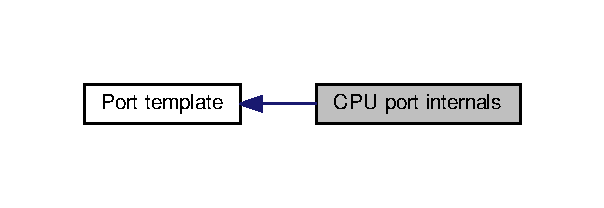
\includegraphics[width=290pt]{group__template__cpu__impl}
\end{center}
\end{figure}
\subsubsection*{Functions}
\begin{DoxyCompactItemize}
\item 
uint\-\_\-fast8\-\_\-t \hyperlink{group__template__cpu__impl_ga548cbf806bfd34904f60a1f8db0ce965}{port\-Find\-Last\-Set\-\_\-} (\hyperlink{group__template__cpu__intf_ga99980ab56ce9857e7380210d12e3d41f}{port\-Reg\-\_\-\-T} val)
\begin{DoxyCompactList}\small\item\em Find last set bit in a word. \end{DoxyCompactList}\item 
void $\ast$ \hyperlink{group__template__cpu__impl_ga91a1dc500f743c80ec573148a99add67}{port\-Ctx\-Init\-\_\-} (void $\ast$stck, size\-\_\-t stck\-Size, void($\ast$fn)(void $\ast$), void $\ast$arg)
\begin{DoxyCompactList}\small\item\em Initialize the thread context. \end{DoxyCompactList}\end{DoxyCompactItemize}
\subsubsection*{Variables}
\begin{DoxyCompactItemize}
\item 
\hyperlink{group__template__cpu__intf_ga99980ab56ce9857e7380210d12e3d41f}{port\-Reg\-\_\-\-T} \hyperlink{group__template__cpu__impl_ga76dd98d1f19ff5ce4b4e880dfcedadb9}{g\-Port\-Isr\-Nesting\-\_\-}
\begin{DoxyCompactList}\small\item\em Variable to keep track of I\-S\-R nesting. \end{DoxyCompactList}\item 
const P\-O\-R\-T\-\_\-\-C\-\_\-\-R\-O\-M \hyperlink{group__template__cpu__intf_ga99980ab56ce9857e7380210d12e3d41f}{port\-Reg\-\_\-\-T} \hyperlink{group__template__cpu__impl_ga7c74d77135d5a694029ce4805f5dbc13}{pwr2\-L\-K\-P} \mbox{[}\hyperlink{group__template__cpu__intf_gac4d9e19c50315dec7721d4bc4d6b0605}{P\-O\-R\-T\-\_\-\-D\-A\-T\-A\-\_\-\-W\-I\-D\-T\-H\-\_\-\-V\-A\-L}\mbox{]}
\begin{DoxyCompactList}\small\item\em Look up table for\-: 2$^\wedge$n expression. \end{DoxyCompactList}\end{DoxyCompactItemize}


\subsubsection{Detailed Description}
C\-P\-U port inner work. 

\subsubsection{Function Documentation}
\hypertarget{group__template__cpu__impl_ga548cbf806bfd34904f60a1f8db0ce965}{\index{C\-P\-U port internals@{C\-P\-U port internals}!port\-Find\-Last\-Set\-\_\-@{port\-Find\-Last\-Set\-\_\-}}
\index{port\-Find\-Last\-Set\-\_\-@{port\-Find\-Last\-Set\-\_\-}!CPU port internals@{C\-P\-U port internals}}
\paragraph[{port\-Find\-Last\-Set\-\_\-}]{\setlength{\rightskip}{0pt plus 5cm}uint\-\_\-fast8\-\_\-t port\-Find\-Last\-Set\-\_\- (
\begin{DoxyParamCaption}
\item[{{\bf port\-Reg\-\_\-\-T}}]{val}
\end{DoxyParamCaption}
)}}\label{group__template__cpu__impl_ga548cbf806bfd34904f60a1f8db0ce965}


Find last set bit in a word. 


\begin{DoxyParams}{Parameters}
{\em val} & Value which needs to be evaluated\\
\hline
\end{DoxyParams}
This function is used by the scheduler to efficiently determine the highest priority of thread ready for execution. For algorithm details see\-: \href{http://en.wikipedia.org/wiki/Find_first_set}{\tt http\-://en.\-wikipedia.\-org/wiki/\-Find\-\_\-first\-\_\-set}. \begin{DoxyReturn}{Returns}
The position of the last set bit in a word 
\end{DoxyReturn}
\hypertarget{group__template__cpu__impl_ga91a1dc500f743c80ec573148a99add67}{\index{C\-P\-U port internals@{C\-P\-U port internals}!port\-Ctx\-Init\-\_\-@{port\-Ctx\-Init\-\_\-}}
\index{port\-Ctx\-Init\-\_\-@{port\-Ctx\-Init\-\_\-}!CPU port internals@{C\-P\-U port internals}}
\paragraph[{port\-Ctx\-Init\-\_\-}]{\setlength{\rightskip}{0pt plus 5cm}void$\ast$ port\-Ctx\-Init\-\_\- (
\begin{DoxyParamCaption}
\item[{void $\ast$}]{stck, }
\item[{size\-\_\-t}]{stck\-Size, }
\item[{void($\ast$)(void $\ast$)}]{fn, }
\item[{void $\ast$}]{arg}
\end{DoxyParamCaption}
)}}\label{group__template__cpu__impl_ga91a1dc500f743c80ec573148a99add67}


Initialize the thread context. 


\begin{DoxyParams}{Parameters}
{\em stck} & Pointer to the allocated thread stck. The pointer points to the beginning of the memory as defined per C language. It's up to port function to adjust the pointer according to the stck type\-: full descending or full ascending one. \\
\hline
{\em stck\-Size} & The size of allocated stck in bytes. \\
\hline
{\em fn} & Pointer to the thread function. \\
\hline
{\em arg} & Argument that will be passed to thread function at the starting of execution. \\
\hline
\end{DoxyParams}
\begin{DoxyReturn}{Returns}
The new top of stck after thread context initialization. 
\end{DoxyReturn}


\subsubsection{Variable Documentation}
\hypertarget{group__template__cpu__impl_ga76dd98d1f19ff5ce4b4e880dfcedadb9}{\index{C\-P\-U port internals@{C\-P\-U port internals}!g\-Port\-Isr\-Nesting\-\_\-@{g\-Port\-Isr\-Nesting\-\_\-}}
\index{g\-Port\-Isr\-Nesting\-\_\-@{g\-Port\-Isr\-Nesting\-\_\-}!CPU port internals@{C\-P\-U port internals}}
\paragraph[{g\-Port\-Isr\-Nesting\-\_\-}]{\setlength{\rightskip}{0pt plus 5cm}{\bf port\-Reg\-\_\-\-T} g\-Port\-Isr\-Nesting\-\_\-}}\label{group__template__cpu__impl_ga76dd98d1f19ff5ce4b4e880dfcedadb9}


Variable to keep track of I\-S\-R nesting. 

\hypertarget{group__template__cpu__impl_ga7c74d77135d5a694029ce4805f5dbc13}{\index{C\-P\-U port internals@{C\-P\-U port internals}!pwr2\-L\-K\-P@{pwr2\-L\-K\-P}}
\index{pwr2\-L\-K\-P@{pwr2\-L\-K\-P}!CPU port internals@{C\-P\-U port internals}}
\paragraph[{pwr2\-L\-K\-P}]{\setlength{\rightskip}{0pt plus 5cm}const P\-O\-R\-T\-\_\-\-C\-\_\-\-R\-O\-M {\bf port\-Reg\-\_\-\-T} pwr2\-L\-K\-P\mbox{[}{\bf P\-O\-R\-T\-\_\-\-D\-A\-T\-A\-\_\-\-W\-I\-D\-T\-H\-\_\-\-V\-A\-L}\mbox{]}}}\label{group__template__cpu__impl_ga7c74d77135d5a694029ce4805f5dbc13}
{\bfseries Initial value\-:}
\begin{DoxyCode}
= \{
    (1U <<  0), (1U <<  1), (1U <<  2), (1U <<  3),
    (1U <<  4), (1U <<  5), (1U <<  6), (1U <<  7),










\}
\end{DoxyCode}


Look up table for\-: 2$^\wedge$n expression. 

This look up table can be used to accelerate the Logical Shift Left operations which are needed to set bits inside the priority bit map. In plain C this operation would be written as\-: {\ttfamily (1\-U $<$$<$ n)}, but in many 8-\/bit C\-P\-Us this operation can be lengthy. If there is a need for faster operation than this table can be used instead of the mentioned C code.

To use the look up table change \hyperlink{group__template__cpu__intf_ga4b938b55e8398b93969cfb7bc64177cd}{P\-O\-R\-T\-\_\-\-P\-W\-R2} macro implementation from\-: {\ttfamily (1\-U $<$$<$ (pwr))} to {\ttfamily pwr2\-L\-K\-P\mbox{[}pwr\mbox{]}} 
\hypertarget{group__template__cpu__cfg}{\subsection{C\-P\-U port configuration}
\label{group__template__cpu__cfg}\index{C\-P\-U port configuration@{C\-P\-U port configuration}}
}


C\-P\-U port specific configuration options.  


Collaboration diagram for C\-P\-U port configuration\-:\nopagebreak
\begin{figure}[H]
\begin{center}
\leavevmode
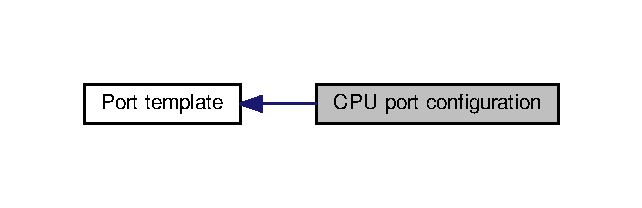
\includegraphics[width=308pt]{group__template__cpu__cfg}
\end{center}
\end{figure}
C\-P\-U port specific configuration options. 
\hypertarget{group__template__family__cfg}{\subsection{Family port configuration}
\label{group__template__family__cfg}\index{Family port configuration@{Family port configuration}}
}


Family port specific configuration options.  


Collaboration diagram for Family port configuration\-:\nopagebreak
\begin{figure}[H]
\begin{center}
\leavevmode
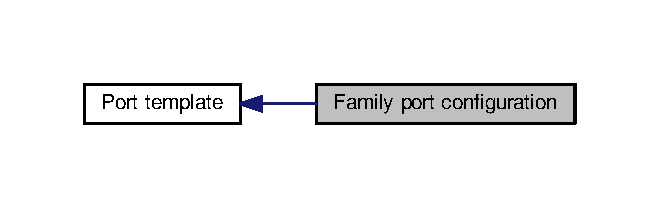
\includegraphics[width=316pt]{group__template__family__cfg}
\end{center}
\end{figure}
\subsubsection*{Generic family defaults}
\begin{DoxyCompactItemize}
\item 
\#define \hyperlink{group__template__family__cfg_gaed6437f330e7be6f8d5a04a19cbe8776}{C\-P\-U\-\_\-\-D\-E\-F\-\_\-\-S\-Y\-S\-T\-M\-R\-\_\-\-M\-A\-X\-\_\-\-V\-A\-L}~0xfful
\begin{DoxyCompactList}\small\item\em System timer maximum value. \end{DoxyCompactList}\end{DoxyCompactItemize}


\subsubsection{Detailed Description}
Family port specific configuration options. 

\subsubsection{Macro Definition Documentation}
\hypertarget{group__template__family__cfg_gaed6437f330e7be6f8d5a04a19cbe8776}{\index{Family port configuration@{Family port configuration}!C\-P\-U\-\_\-\-D\-E\-F\-\_\-\-S\-Y\-S\-T\-M\-R\-\_\-\-M\-A\-X\-\_\-\-V\-A\-L@{C\-P\-U\-\_\-\-D\-E\-F\-\_\-\-S\-Y\-S\-T\-M\-R\-\_\-\-M\-A\-X\-\_\-\-V\-A\-L}}
\index{C\-P\-U\-\_\-\-D\-E\-F\-\_\-\-S\-Y\-S\-T\-M\-R\-\_\-\-M\-A\-X\-\_\-\-V\-A\-L@{C\-P\-U\-\_\-\-D\-E\-F\-\_\-\-S\-Y\-S\-T\-M\-R\-\_\-\-M\-A\-X\-\_\-\-V\-A\-L}!Family port configuration@{Family port configuration}}
\paragraph[{C\-P\-U\-\_\-\-D\-E\-F\-\_\-\-S\-Y\-S\-T\-M\-R\-\_\-\-M\-A\-X\-\_\-\-V\-A\-L}]{\setlength{\rightskip}{0pt plus 5cm}\#define C\-P\-U\-\_\-\-D\-E\-F\-\_\-\-S\-Y\-S\-T\-M\-R\-\_\-\-M\-A\-X\-\_\-\-V\-A\-L~0xfful}}\label{group__template__family__cfg_gaed6437f330e7be6f8d5a04a19cbe8776}


System timer maximum value. 

This macro specifies maximum value that can be reloaded into system timer counter. For example, if the system timer is an 8-\/bit counter than this macro would have the value of 0xffu (255). 
\hypertarget{group__template__kern__cfg}{\subsection{Default Kernel configuration}
\label{group__template__kern__cfg}\index{Default Kernel configuration@{Default Kernel configuration}}
}


Default Kernel Configuration settings.  


Collaboration diagram for Default Kernel configuration\-:\nopagebreak
\begin{figure}[H]
\begin{center}
\leavevmode
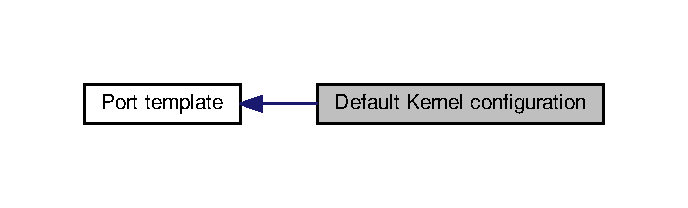
\includegraphics[width=330pt]{group__template__kern__cfg}
\end{center}
\end{figure}
\subsubsection*{Kernel configuration options and settings}
\label{_amgrpb927dce21981a007b6ce68c2f03fc275}%
Kernel default configuration \begin{DoxyCompactItemize}
\item 
\#define \hyperlink{group__template__kern__cfg_ga56bd89fe76f7fe22f3d8805bc3c68892}{C\-F\-G\-\_\-\-S\-C\-H\-E\-D\-\_\-\-P\-R\-I\-O\-\_\-\-L\-V\-L}~8\-U
\begin{DoxyCompactList}\small\item\em Scheduler priority levels. \end{DoxyCompactList}\item 
\#define \hyperlink{group__template__kern__cfg_ga0bd286f16bb67585f14c4d1e45be8ad1}{C\-F\-G\-\_\-\-S\-C\-H\-E\-D\-\_\-\-T\-I\-M\-E\-\_\-\-Q\-U\-A\-N\-T\-U\-M}~10\-U
\begin{DoxyCompactList}\small\item\em Scheduler Round-\/\-Robin time quantum. \end{DoxyCompactList}\item 
\#define \hyperlink{group__template__kern__cfg_ga4e6ab4994b34501bb71e75717b093376}{C\-F\-G\-\_\-\-S\-C\-H\-E\-D\-\_\-\-P\-O\-W\-E\-R\-\_\-\-S\-A\-V\-E}~0\-U
\begin{DoxyCompactList}\small\item\em Enable/disable scheduler power savings mode. \end{DoxyCompactList}\item 
\#define \hyperlink{group__template__kern__cfg_ga5f07eea2a4be92cf0358f52eba6800c9}{C\-F\-G\-\_\-\-S\-Y\-S\-T\-M\-R\-\_\-\-A\-D\-A\-P\-T\-I\-V\-E\-\_\-\-M\-O\-D\-E}~0\-U
\begin{DoxyCompactList}\small\item\em System timer mode. \end{DoxyCompactList}\item 
\#define \hyperlink{group__template__kern__cfg_ga4e46164ae5a37bfc54c67b6f01d93eb1}{C\-F\-G\-\_\-\-S\-Y\-S\-T\-M\-R\-\_\-\-E\-V\-E\-N\-T\-\_\-\-F\-R\-E\-Q\-U\-E\-N\-C\-Y}~100\-U\-L
\begin{DoxyCompactList}\small\item\em The frequency of system tick event. \end{DoxyCompactList}\item 
\#define \hyperlink{group__template__kern__cfg_gad69eef523459c5ab485ce2f62bddceca}{C\-F\-G\-\_\-\-S\-Y\-S\-T\-M\-R\-\_\-\-T\-I\-C\-K\-\_\-\-T\-Y\-P\-E}~2\-U
\begin{DoxyCompactList}\small\item\em The size of the system timer counter. \end{DoxyCompactList}\end{DoxyCompactItemize}
\subsubsection*{Kernel hooks}
\begin{DoxyCompactItemize}
\item 
\#define \hyperlink{group__template__kern__cfg_gaa130bc9f72010b44b4b06618d8f8d0bc}{C\-F\-G\-\_\-\-H\-O\-O\-K\-\_\-\-P\-R\-E\-\_\-\-S\-Y\-S\-T\-M\-R\-\_\-\-E\-V\-E\-N\-T}~0\-U
\begin{DoxyCompactList}\small\item\em System timer event hook function. \end{DoxyCompactList}\item 
\#define \hyperlink{group__template__kern__cfg_ga4093113f2105d2716f86c6509a6e643a}{C\-F\-G\-\_\-\-H\-O\-O\-K\-\_\-\-P\-R\-E\-\_\-\-K\-E\-R\-N\-\_\-\-I\-N\-I\-T}~0\-U
\begin{DoxyCompactList}\small\item\em Pre kernel initialization hook function. \end{DoxyCompactList}\item 
\#define \hyperlink{group__template__kern__cfg_ga85dea823714335c2ec9e9f7750996e83}{C\-F\-G\-\_\-\-H\-O\-O\-K\-\_\-\-P\-O\-S\-T\-\_\-\-K\-E\-R\-N\-\_\-\-I\-N\-I\-T}~0\-U
\begin{DoxyCompactList}\small\item\em Post kernel initialization hook function. \end{DoxyCompactList}\item 
\#define \hyperlink{group__template__kern__cfg_gad67d998118375811b0f3e63543311661}{C\-F\-G\-\_\-\-H\-O\-O\-K\-\_\-\-P\-R\-E\-\_\-\-K\-E\-R\-N\-\_\-\-S\-T\-A\-R\-T}~0\-U
\begin{DoxyCompactList}\small\item\em Pre kernel start hook function. \end{DoxyCompactList}\item 
\#define \hyperlink{group__template__kern__cfg_ga23deae306171d1a8dda4d0e33efdb6bb}{C\-F\-G\-\_\-\-H\-O\-O\-K\-\_\-\-P\-O\-S\-T\-\_\-\-T\-H\-D\-\_\-\-I\-N\-I\-T}~0\-U
\begin{DoxyCompactList}\small\item\em Post thread initialization hook function. \end{DoxyCompactList}\item 
\#define \hyperlink{group__template__kern__cfg_ga9c7dd4e009a89e9cffb0f9b404bc6250}{C\-F\-G\-\_\-\-H\-O\-O\-K\-\_\-\-P\-R\-E\-\_\-\-T\-H\-D\-\_\-\-T\-E\-R\-M}~0\-U
\begin{DoxyCompactList}\small\item\em Pre thread termination hook function. \end{DoxyCompactList}\item 
\#define \hyperlink{group__template__kern__cfg_ga7c2b0410404256c4804758090401f7e4}{C\-F\-G\-\_\-\-H\-O\-O\-K\-\_\-\-P\-R\-E\-\_\-\-I\-D\-L\-E}~0\-U
\begin{DoxyCompactList}\small\item\em Pre idle hook function. \end{DoxyCompactList}\item 
\#define \hyperlink{group__template__kern__cfg_ga8f8751efe94964bef25673deca6b9b26}{C\-F\-G\-\_\-\-H\-O\-O\-K\-\_\-\-P\-O\-S\-T\-\_\-\-I\-D\-L\-E}~0\-U
\begin{DoxyCompactList}\small\item\em Post idle hook function. \end{DoxyCompactList}\item 
\#define \hyperlink{group__template__kern__cfg_gac84acbf84222018398089920dd429635}{C\-F\-G\-\_\-\-H\-O\-O\-K\-\_\-\-P\-R\-E\-\_\-\-C\-T\-X\-\_\-\-S\-W}~0\-U
\begin{DoxyCompactList}\small\item\em Pre context switch hook function. \end{DoxyCompactList}\end{DoxyCompactItemize}


\subsubsection{Detailed Description}
Default Kernel Configuration settings. Each configuration option or setting has its own default value when not defined by the application. When application needs to change a setting it just needs to define a configuration macro with another value and the default configuration macro will be overridden. 

\subsubsection{Macro Definition Documentation}
\hypertarget{group__template__kern__cfg_ga56bd89fe76f7fe22f3d8805bc3c68892}{\index{Default Kernel configuration@{Default Kernel configuration}!C\-F\-G\-\_\-\-S\-C\-H\-E\-D\-\_\-\-P\-R\-I\-O\-\_\-\-L\-V\-L@{C\-F\-G\-\_\-\-S\-C\-H\-E\-D\-\_\-\-P\-R\-I\-O\-\_\-\-L\-V\-L}}
\index{C\-F\-G\-\_\-\-S\-C\-H\-E\-D\-\_\-\-P\-R\-I\-O\-\_\-\-L\-V\-L@{C\-F\-G\-\_\-\-S\-C\-H\-E\-D\-\_\-\-P\-R\-I\-O\-\_\-\-L\-V\-L}!Default Kernel configuration@{Default Kernel configuration}}
\paragraph[{C\-F\-G\-\_\-\-S\-C\-H\-E\-D\-\_\-\-P\-R\-I\-O\-\_\-\-L\-V\-L}]{\setlength{\rightskip}{0pt plus 5cm}\#define C\-F\-G\-\_\-\-S\-C\-H\-E\-D\-\_\-\-P\-R\-I\-O\-\_\-\-L\-V\-L~8\-U}}\label{group__template__kern__cfg_ga56bd89fe76f7fe22f3d8805bc3c68892}


Scheduler priority levels. 

The number of priority levels. Each priority level can have several threads. Possible values\-:
\begin{DoxyItemize}
\item Min\-: 3\-U (three priority levels)
\item Max\-: 256\-U 
\end{DoxyItemize}\hypertarget{group__template__kern__cfg_ga0bd286f16bb67585f14c4d1e45be8ad1}{\index{Default Kernel configuration@{Default Kernel configuration}!C\-F\-G\-\_\-\-S\-C\-H\-E\-D\-\_\-\-T\-I\-M\-E\-\_\-\-Q\-U\-A\-N\-T\-U\-M@{C\-F\-G\-\_\-\-S\-C\-H\-E\-D\-\_\-\-T\-I\-M\-E\-\_\-\-Q\-U\-A\-N\-T\-U\-M}}
\index{C\-F\-G\-\_\-\-S\-C\-H\-E\-D\-\_\-\-T\-I\-M\-E\-\_\-\-Q\-U\-A\-N\-T\-U\-M@{C\-F\-G\-\_\-\-S\-C\-H\-E\-D\-\_\-\-T\-I\-M\-E\-\_\-\-Q\-U\-A\-N\-T\-U\-M}!Default Kernel configuration@{Default Kernel configuration}}
\paragraph[{C\-F\-G\-\_\-\-S\-C\-H\-E\-D\-\_\-\-T\-I\-M\-E\-\_\-\-Q\-U\-A\-N\-T\-U\-M}]{\setlength{\rightskip}{0pt plus 5cm}\#define C\-F\-G\-\_\-\-S\-C\-H\-E\-D\-\_\-\-T\-I\-M\-E\-\_\-\-Q\-U\-A\-N\-T\-U\-M~10\-U}}\label{group__template__kern__cfg_ga0bd286f16bb67585f14c4d1e45be8ad1}


Scheduler Round-\/\-Robin time quantum. 

This constant is the number of system ticks allowed for the threads before preemption occurs. Setting this value to zero disables the preemption for threads with equal priority and the round robin becomes cooperative. Note that higher priority threads can still preempt, the kernel is always preemptive. \begin{DoxyNote}{Note}
Disabling the round robin preemption makes the kernel more compact and generally faster. 
\end{DoxyNote}
\hypertarget{group__template__kern__cfg_ga4e6ab4994b34501bb71e75717b093376}{\index{Default Kernel configuration@{Default Kernel configuration}!C\-F\-G\-\_\-\-S\-C\-H\-E\-D\-\_\-\-P\-O\-W\-E\-R\-\_\-\-S\-A\-V\-E@{C\-F\-G\-\_\-\-S\-C\-H\-E\-D\-\_\-\-P\-O\-W\-E\-R\-\_\-\-S\-A\-V\-E}}
\index{C\-F\-G\-\_\-\-S\-C\-H\-E\-D\-\_\-\-P\-O\-W\-E\-R\-\_\-\-S\-A\-V\-E@{C\-F\-G\-\_\-\-S\-C\-H\-E\-D\-\_\-\-P\-O\-W\-E\-R\-\_\-\-S\-A\-V\-E}!Default Kernel configuration@{Default Kernel configuration}}
\paragraph[{C\-F\-G\-\_\-\-S\-C\-H\-E\-D\-\_\-\-P\-O\-W\-E\-R\-\_\-\-S\-A\-V\-E}]{\setlength{\rightskip}{0pt plus 5cm}\#define C\-F\-G\-\_\-\-S\-C\-H\-E\-D\-\_\-\-P\-O\-W\-E\-R\-\_\-\-S\-A\-V\-E~0\-U}}\label{group__template__kern__cfg_ga4e6ab4994b34501bb71e75717b093376}


Enable/disable scheduler power savings mode. 

Possible values are\-:
\begin{DoxyItemize}
\item 0\-U -\/ power saving is disabled
\item 1\-U -\/ power saving is enabled 
\end{DoxyItemize}\hypertarget{group__template__kern__cfg_ga5f07eea2a4be92cf0358f52eba6800c9}{\index{Default Kernel configuration@{Default Kernel configuration}!C\-F\-G\-\_\-\-S\-Y\-S\-T\-M\-R\-\_\-\-A\-D\-A\-P\-T\-I\-V\-E\-\_\-\-M\-O\-D\-E@{C\-F\-G\-\_\-\-S\-Y\-S\-T\-M\-R\-\_\-\-A\-D\-A\-P\-T\-I\-V\-E\-\_\-\-M\-O\-D\-E}}
\index{C\-F\-G\-\_\-\-S\-Y\-S\-T\-M\-R\-\_\-\-A\-D\-A\-P\-T\-I\-V\-E\-\_\-\-M\-O\-D\-E@{C\-F\-G\-\_\-\-S\-Y\-S\-T\-M\-R\-\_\-\-A\-D\-A\-P\-T\-I\-V\-E\-\_\-\-M\-O\-D\-E}!Default Kernel configuration@{Default Kernel configuration}}
\paragraph[{C\-F\-G\-\_\-\-S\-Y\-S\-T\-M\-R\-\_\-\-A\-D\-A\-P\-T\-I\-V\-E\-\_\-\-M\-O\-D\-E}]{\setlength{\rightskip}{0pt plus 5cm}\#define C\-F\-G\-\_\-\-S\-Y\-S\-T\-M\-R\-\_\-\-A\-D\-A\-P\-T\-I\-V\-E\-\_\-\-M\-O\-D\-E~0\-U}}\label{group__template__kern__cfg_ga5f07eea2a4be92cf0358f52eba6800c9}


System timer mode. 

Possible values are\-:
\begin{DoxyItemize}
\item 0\-U -\/ adaptive mode is disabled
\item 1\-U -\/ adaptive mode is enabled 
\end{DoxyItemize}\hypertarget{group__template__kern__cfg_ga4e46164ae5a37bfc54c67b6f01d93eb1}{\index{Default Kernel configuration@{Default Kernel configuration}!C\-F\-G\-\_\-\-S\-Y\-S\-T\-M\-R\-\_\-\-E\-V\-E\-N\-T\-\_\-\-F\-R\-E\-Q\-U\-E\-N\-C\-Y@{C\-F\-G\-\_\-\-S\-Y\-S\-T\-M\-R\-\_\-\-E\-V\-E\-N\-T\-\_\-\-F\-R\-E\-Q\-U\-E\-N\-C\-Y}}
\index{C\-F\-G\-\_\-\-S\-Y\-S\-T\-M\-R\-\_\-\-E\-V\-E\-N\-T\-\_\-\-F\-R\-E\-Q\-U\-E\-N\-C\-Y@{C\-F\-G\-\_\-\-S\-Y\-S\-T\-M\-R\-\_\-\-E\-V\-E\-N\-T\-\_\-\-F\-R\-E\-Q\-U\-E\-N\-C\-Y}!Default Kernel configuration@{Default Kernel configuration}}
\paragraph[{C\-F\-G\-\_\-\-S\-Y\-S\-T\-M\-R\-\_\-\-E\-V\-E\-N\-T\-\_\-\-F\-R\-E\-Q\-U\-E\-N\-C\-Y}]{\setlength{\rightskip}{0pt plus 5cm}\#define C\-F\-G\-\_\-\-S\-Y\-S\-T\-M\-R\-\_\-\-E\-V\-E\-N\-T\-\_\-\-F\-R\-E\-Q\-U\-E\-N\-C\-Y~100\-U\-L}}\label{group__template__kern__cfg_ga4e46164ae5a37bfc54c67b6f01d93eb1}


The frequency of system tick event. 

Specify the desired resolution system tick time source. This setting is valid only if configuration option \hyperlink{group__template__cpu__cfg_gac85c592962ba2c968d13f867533196a1}{C\-F\-G\-\_\-\-S\-Y\-S\-T\-M\-R\-\_\-\-C\-L\-O\-C\-K\-\_\-\-F\-R\-E\-Q\-U\-E\-N\-C\-Y} is properly set in port configuration file \hyperlink{cpu__cfg_8h}{cpu\-\_\-cfg.\-h} \hypertarget{group__template__kern__cfg_gad69eef523459c5ab485ce2f62bddceca}{\index{Default Kernel configuration@{Default Kernel configuration}!C\-F\-G\-\_\-\-S\-Y\-S\-T\-M\-R\-\_\-\-T\-I\-C\-K\-\_\-\-T\-Y\-P\-E@{C\-F\-G\-\_\-\-S\-Y\-S\-T\-M\-R\-\_\-\-T\-I\-C\-K\-\_\-\-T\-Y\-P\-E}}
\index{C\-F\-G\-\_\-\-S\-Y\-S\-T\-M\-R\-\_\-\-T\-I\-C\-K\-\_\-\-T\-Y\-P\-E@{C\-F\-G\-\_\-\-S\-Y\-S\-T\-M\-R\-\_\-\-T\-I\-C\-K\-\_\-\-T\-Y\-P\-E}!Default Kernel configuration@{Default Kernel configuration}}
\paragraph[{C\-F\-G\-\_\-\-S\-Y\-S\-T\-M\-R\-\_\-\-T\-I\-C\-K\-\_\-\-T\-Y\-P\-E}]{\setlength{\rightskip}{0pt plus 5cm}\#define C\-F\-G\-\_\-\-S\-Y\-S\-T\-M\-R\-\_\-\-T\-I\-C\-K\-\_\-\-T\-Y\-P\-E~2\-U}}\label{group__template__kern__cfg_gad69eef523459c5ab485ce2f62bddceca}


The size of the system timer counter. 

Possible values are\-:
\begin{DoxyItemize}
\item 0\-U -\/ 8 bit counter
\item 1\-U -\/ 16 bit counter
\item 2\-U -\/ 32 bit counter 
\end{DoxyItemize}\hypertarget{group__template__kern__cfg_gaa130bc9f72010b44b4b06618d8f8d0bc}{\index{Default Kernel configuration@{Default Kernel configuration}!C\-F\-G\-\_\-\-H\-O\-O\-K\-\_\-\-P\-R\-E\-\_\-\-S\-Y\-S\-T\-M\-R\-\_\-\-E\-V\-E\-N\-T@{C\-F\-G\-\_\-\-H\-O\-O\-K\-\_\-\-P\-R\-E\-\_\-\-S\-Y\-S\-T\-M\-R\-\_\-\-E\-V\-E\-N\-T}}
\index{C\-F\-G\-\_\-\-H\-O\-O\-K\-\_\-\-P\-R\-E\-\_\-\-S\-Y\-S\-T\-M\-R\-\_\-\-E\-V\-E\-N\-T@{C\-F\-G\-\_\-\-H\-O\-O\-K\-\_\-\-P\-R\-E\-\_\-\-S\-Y\-S\-T\-M\-R\-\_\-\-E\-V\-E\-N\-T}!Default Kernel configuration@{Default Kernel configuration}}
\paragraph[{C\-F\-G\-\_\-\-H\-O\-O\-K\-\_\-\-P\-R\-E\-\_\-\-S\-Y\-S\-T\-M\-R\-\_\-\-E\-V\-E\-N\-T}]{\setlength{\rightskip}{0pt plus 5cm}\#define C\-F\-G\-\_\-\-H\-O\-O\-K\-\_\-\-P\-R\-E\-\_\-\-S\-Y\-S\-T\-M\-R\-\_\-\-E\-V\-E\-N\-T~0\-U}}\label{group__template__kern__cfg_gaa130bc9f72010b44b4b06618d8f8d0bc}


System timer event hook function. 

This hook is called just a moment before a system timer event is processed. \begin{DoxyNote}{Note}
This hook will call \hyperlink{group__kern__intf_ga9a0d562969acef0121136b11be7b4728}{user\-Pre\-Sys\-Tmr()} function. 
\end{DoxyNote}
\hypertarget{group__template__kern__cfg_ga4093113f2105d2716f86c6509a6e643a}{\index{Default Kernel configuration@{Default Kernel configuration}!C\-F\-G\-\_\-\-H\-O\-O\-K\-\_\-\-P\-R\-E\-\_\-\-K\-E\-R\-N\-\_\-\-I\-N\-I\-T@{C\-F\-G\-\_\-\-H\-O\-O\-K\-\_\-\-P\-R\-E\-\_\-\-K\-E\-R\-N\-\_\-\-I\-N\-I\-T}}
\index{C\-F\-G\-\_\-\-H\-O\-O\-K\-\_\-\-P\-R\-E\-\_\-\-K\-E\-R\-N\-\_\-\-I\-N\-I\-T@{C\-F\-G\-\_\-\-H\-O\-O\-K\-\_\-\-P\-R\-E\-\_\-\-K\-E\-R\-N\-\_\-\-I\-N\-I\-T}!Default Kernel configuration@{Default Kernel configuration}}
\paragraph[{C\-F\-G\-\_\-\-H\-O\-O\-K\-\_\-\-P\-R\-E\-\_\-\-K\-E\-R\-N\-\_\-\-I\-N\-I\-T}]{\setlength{\rightskip}{0pt plus 5cm}\#define C\-F\-G\-\_\-\-H\-O\-O\-K\-\_\-\-P\-R\-E\-\_\-\-K\-E\-R\-N\-\_\-\-I\-N\-I\-T~0\-U}}\label{group__template__kern__cfg_ga4093113f2105d2716f86c6509a6e643a}


Pre kernel initialization hook function. 

This hook is called at the beginning of \hyperlink{group__kern__intf_ga9e9ff699d62d6035cd51121bb3140704}{es\-Kern\-Init()} function. \begin{DoxyNote}{Note}
This hook will call \hyperlink{group__kern__intf_gaac77966856c9a299cda4794cbcc87edf}{user\-Pre\-Kern\-Init()} function. 
\end{DoxyNote}
\hypertarget{group__template__kern__cfg_ga85dea823714335c2ec9e9f7750996e83}{\index{Default Kernel configuration@{Default Kernel configuration}!C\-F\-G\-\_\-\-H\-O\-O\-K\-\_\-\-P\-O\-S\-T\-\_\-\-K\-E\-R\-N\-\_\-\-I\-N\-I\-T@{C\-F\-G\-\_\-\-H\-O\-O\-K\-\_\-\-P\-O\-S\-T\-\_\-\-K\-E\-R\-N\-\_\-\-I\-N\-I\-T}}
\index{C\-F\-G\-\_\-\-H\-O\-O\-K\-\_\-\-P\-O\-S\-T\-\_\-\-K\-E\-R\-N\-\_\-\-I\-N\-I\-T@{C\-F\-G\-\_\-\-H\-O\-O\-K\-\_\-\-P\-O\-S\-T\-\_\-\-K\-E\-R\-N\-\_\-\-I\-N\-I\-T}!Default Kernel configuration@{Default Kernel configuration}}
\paragraph[{C\-F\-G\-\_\-\-H\-O\-O\-K\-\_\-\-P\-O\-S\-T\-\_\-\-K\-E\-R\-N\-\_\-\-I\-N\-I\-T}]{\setlength{\rightskip}{0pt plus 5cm}\#define C\-F\-G\-\_\-\-H\-O\-O\-K\-\_\-\-P\-O\-S\-T\-\_\-\-K\-E\-R\-N\-\_\-\-I\-N\-I\-T~0\-U}}\label{group__template__kern__cfg_ga85dea823714335c2ec9e9f7750996e83}


Post kernel initialization hook function. 

\begin{DoxyNote}{Note}
This hook will call \hyperlink{group__kern__intf_ga3579ac6964a314ad03d13da0507f57e8}{user\-Post\-Kern\-Init()} function. 
\end{DoxyNote}
\hypertarget{group__template__kern__cfg_gad67d998118375811b0f3e63543311661}{\index{Default Kernel configuration@{Default Kernel configuration}!C\-F\-G\-\_\-\-H\-O\-O\-K\-\_\-\-P\-R\-E\-\_\-\-K\-E\-R\-N\-\_\-\-S\-T\-A\-R\-T@{C\-F\-G\-\_\-\-H\-O\-O\-K\-\_\-\-P\-R\-E\-\_\-\-K\-E\-R\-N\-\_\-\-S\-T\-A\-R\-T}}
\index{C\-F\-G\-\_\-\-H\-O\-O\-K\-\_\-\-P\-R\-E\-\_\-\-K\-E\-R\-N\-\_\-\-S\-T\-A\-R\-T@{C\-F\-G\-\_\-\-H\-O\-O\-K\-\_\-\-P\-R\-E\-\_\-\-K\-E\-R\-N\-\_\-\-S\-T\-A\-R\-T}!Default Kernel configuration@{Default Kernel configuration}}
\paragraph[{C\-F\-G\-\_\-\-H\-O\-O\-K\-\_\-\-P\-R\-E\-\_\-\-K\-E\-R\-N\-\_\-\-S\-T\-A\-R\-T}]{\setlength{\rightskip}{0pt plus 5cm}\#define C\-F\-G\-\_\-\-H\-O\-O\-K\-\_\-\-P\-R\-E\-\_\-\-K\-E\-R\-N\-\_\-\-S\-T\-A\-R\-T~0\-U}}\label{group__template__kern__cfg_gad67d998118375811b0f3e63543311661}


Pre kernel start hook function. 

This hook is called at the beginning of \hyperlink{group__kern__intf_ga0e7a0a6b9c02df58de0f98de0229a09d}{es\-Kern\-Start()} function. \begin{DoxyNote}{Note}
This hook will call \hyperlink{group__kern__intf_gaac505ab4c72e0fb346ca441d6def327d}{user\-Pre\-Kern\-Start()} function. 
\end{DoxyNote}
\hypertarget{group__template__kern__cfg_ga23deae306171d1a8dda4d0e33efdb6bb}{\index{Default Kernel configuration@{Default Kernel configuration}!C\-F\-G\-\_\-\-H\-O\-O\-K\-\_\-\-P\-O\-S\-T\-\_\-\-T\-H\-D\-\_\-\-I\-N\-I\-T@{C\-F\-G\-\_\-\-H\-O\-O\-K\-\_\-\-P\-O\-S\-T\-\_\-\-T\-H\-D\-\_\-\-I\-N\-I\-T}}
\index{C\-F\-G\-\_\-\-H\-O\-O\-K\-\_\-\-P\-O\-S\-T\-\_\-\-T\-H\-D\-\_\-\-I\-N\-I\-T@{C\-F\-G\-\_\-\-H\-O\-O\-K\-\_\-\-P\-O\-S\-T\-\_\-\-T\-H\-D\-\_\-\-I\-N\-I\-T}!Default Kernel configuration@{Default Kernel configuration}}
\paragraph[{C\-F\-G\-\_\-\-H\-O\-O\-K\-\_\-\-P\-O\-S\-T\-\_\-\-T\-H\-D\-\_\-\-I\-N\-I\-T}]{\setlength{\rightskip}{0pt plus 5cm}\#define C\-F\-G\-\_\-\-H\-O\-O\-K\-\_\-\-P\-O\-S\-T\-\_\-\-T\-H\-D\-\_\-\-I\-N\-I\-T~0\-U}}\label{group__template__kern__cfg_ga23deae306171d1a8dda4d0e33efdb6bb}


Post thread initialization hook function. 

This hook is called at the end of \hyperlink{group__kern__intf_gac91734f3ee867b519f59bf81cc7fde88}{es\-Thd\-Init()} function. \begin{DoxyNote}{Note}
This hook will call \hyperlink{group__kern__intf_ga64ca864d0ff2aaa532208d7c2b88bdb3}{user\-Post\-Thd\-Init()} function. 
\end{DoxyNote}
\hypertarget{group__template__kern__cfg_ga9c7dd4e009a89e9cffb0f9b404bc6250}{\index{Default Kernel configuration@{Default Kernel configuration}!C\-F\-G\-\_\-\-H\-O\-O\-K\-\_\-\-P\-R\-E\-\_\-\-T\-H\-D\-\_\-\-T\-E\-R\-M@{C\-F\-G\-\_\-\-H\-O\-O\-K\-\_\-\-P\-R\-E\-\_\-\-T\-H\-D\-\_\-\-T\-E\-R\-M}}
\index{C\-F\-G\-\_\-\-H\-O\-O\-K\-\_\-\-P\-R\-E\-\_\-\-T\-H\-D\-\_\-\-T\-E\-R\-M@{C\-F\-G\-\_\-\-H\-O\-O\-K\-\_\-\-P\-R\-E\-\_\-\-T\-H\-D\-\_\-\-T\-E\-R\-M}!Default Kernel configuration@{Default Kernel configuration}}
\paragraph[{C\-F\-G\-\_\-\-H\-O\-O\-K\-\_\-\-P\-R\-E\-\_\-\-T\-H\-D\-\_\-\-T\-E\-R\-M}]{\setlength{\rightskip}{0pt plus 5cm}\#define C\-F\-G\-\_\-\-H\-O\-O\-K\-\_\-\-P\-R\-E\-\_\-\-T\-H\-D\-\_\-\-T\-E\-R\-M~0\-U}}\label{group__template__kern__cfg_ga9c7dd4e009a89e9cffb0f9b404bc6250}


Pre thread termination hook function. 

This hook is called when a thread terminates. \begin{DoxyNote}{Note}
This hook will call \hyperlink{group__kern__intf_ga076ad76633999c9d5e245e3b5c6e0c09}{user\-Pre\-Thd\-Term()} function. 
\end{DoxyNote}
\hypertarget{group__template__kern__cfg_ga7c2b0410404256c4804758090401f7e4}{\index{Default Kernel configuration@{Default Kernel configuration}!C\-F\-G\-\_\-\-H\-O\-O\-K\-\_\-\-P\-R\-E\-\_\-\-I\-D\-L\-E@{C\-F\-G\-\_\-\-H\-O\-O\-K\-\_\-\-P\-R\-E\-\_\-\-I\-D\-L\-E}}
\index{C\-F\-G\-\_\-\-H\-O\-O\-K\-\_\-\-P\-R\-E\-\_\-\-I\-D\-L\-E@{C\-F\-G\-\_\-\-H\-O\-O\-K\-\_\-\-P\-R\-E\-\_\-\-I\-D\-L\-E}!Default Kernel configuration@{Default Kernel configuration}}
\paragraph[{C\-F\-G\-\_\-\-H\-O\-O\-K\-\_\-\-P\-R\-E\-\_\-\-I\-D\-L\-E}]{\setlength{\rightskip}{0pt plus 5cm}\#define C\-F\-G\-\_\-\-H\-O\-O\-K\-\_\-\-P\-R\-E\-\_\-\-I\-D\-L\-E~0\-U}}\label{group__template__kern__cfg_ga7c2b0410404256c4804758090401f7e4}


Pre idle hook function. 

\begin{DoxyNote}{Note}
This hook will call \hyperlink{group__kern__intf_ga2bd40d82f768787c3dab2f4df336685e}{user\-Pre\-Idle()} function. 
\end{DoxyNote}
\hypertarget{group__template__kern__cfg_ga8f8751efe94964bef25673deca6b9b26}{\index{Default Kernel configuration@{Default Kernel configuration}!C\-F\-G\-\_\-\-H\-O\-O\-K\-\_\-\-P\-O\-S\-T\-\_\-\-I\-D\-L\-E@{C\-F\-G\-\_\-\-H\-O\-O\-K\-\_\-\-P\-O\-S\-T\-\_\-\-I\-D\-L\-E}}
\index{C\-F\-G\-\_\-\-H\-O\-O\-K\-\_\-\-P\-O\-S\-T\-\_\-\-I\-D\-L\-E@{C\-F\-G\-\_\-\-H\-O\-O\-K\-\_\-\-P\-O\-S\-T\-\_\-\-I\-D\-L\-E}!Default Kernel configuration@{Default Kernel configuration}}
\paragraph[{C\-F\-G\-\_\-\-H\-O\-O\-K\-\_\-\-P\-O\-S\-T\-\_\-\-I\-D\-L\-E}]{\setlength{\rightskip}{0pt plus 5cm}\#define C\-F\-G\-\_\-\-H\-O\-O\-K\-\_\-\-P\-O\-S\-T\-\_\-\-I\-D\-L\-E~0\-U}}\label{group__template__kern__cfg_ga8f8751efe94964bef25673deca6b9b26}


Post idle hook function. 

\begin{DoxyNote}{Note}
This hook will call \hyperlink{group__kern__intf_ga7ca4a96cbe5064d633298d1d172fd4e7}{user\-Post\-Idle()} function. 
\end{DoxyNote}
\hypertarget{group__template__kern__cfg_gac84acbf84222018398089920dd429635}{\index{Default Kernel configuration@{Default Kernel configuration}!C\-F\-G\-\_\-\-H\-O\-O\-K\-\_\-\-P\-R\-E\-\_\-\-C\-T\-X\-\_\-\-S\-W@{C\-F\-G\-\_\-\-H\-O\-O\-K\-\_\-\-P\-R\-E\-\_\-\-C\-T\-X\-\_\-\-S\-W}}
\index{C\-F\-G\-\_\-\-H\-O\-O\-K\-\_\-\-P\-R\-E\-\_\-\-C\-T\-X\-\_\-\-S\-W@{C\-F\-G\-\_\-\-H\-O\-O\-K\-\_\-\-P\-R\-E\-\_\-\-C\-T\-X\-\_\-\-S\-W}!Default Kernel configuration@{Default Kernel configuration}}
\paragraph[{C\-F\-G\-\_\-\-H\-O\-O\-K\-\_\-\-P\-R\-E\-\_\-\-C\-T\-X\-\_\-\-S\-W}]{\setlength{\rightskip}{0pt plus 5cm}\#define C\-F\-G\-\_\-\-H\-O\-O\-K\-\_\-\-P\-R\-E\-\_\-\-C\-T\-X\-\_\-\-S\-W~0\-U}}\label{group__template__kern__cfg_gac84acbf84222018398089920dd429635}


Pre context switch hook function. 

This hook is called before each context switch. \begin{DoxyNote}{Note}
This hook will call \hyperlink{group__kern__intf_ga74a38c965110d0f2f2e44e13571fe3fc}{user\-Pre\-Ctx\-Sw()} function. 
\end{DoxyNote}

\hypertarget{group__template__dbg__cfg}{\subsection{Default Debug configuration}
\label{group__template__dbg__cfg}\index{Default Debug configuration@{Default Debug configuration}}
}


Default Debug Configuration settings.  


Collaboration diagram for Default Debug configuration\-:\nopagebreak
\begin{figure}[H]
\begin{center}
\leavevmode
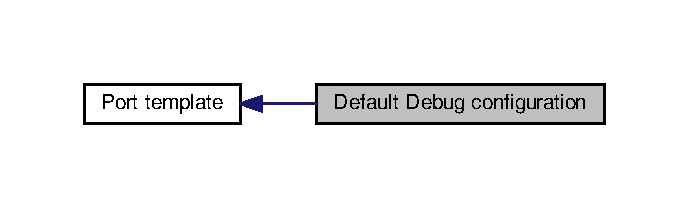
\includegraphics[width=330pt]{group__template__dbg__cfg}
\end{center}
\end{figure}
\subsubsection*{Macros}
\begin{DoxyCompactItemize}
\item 
\#define \hyperlink{group__template__dbg__cfg_ga2ee37a5fa7efdba7d0014328e6c623a8}{C\-F\-G\-\_\-\-D\-B\-G\-\_\-\-E\-N\-A\-B\-L\-E}~1\-U
\begin{DoxyCompactList}\small\item\em Enable/disable Debug module. \end{DoxyCompactList}\item 
\#define \hyperlink{group__template__dbg__cfg_ga64e39c477ef9d900b82585150329e3f0}{C\-F\-G\-\_\-\-D\-B\-G\-\_\-\-A\-P\-I\-\_\-\-V\-A\-L\-I\-D\-A\-T\-I\-O\-N}~1\-U
\begin{DoxyCompactList}\small\item\em Enable/disable A\-P\-I arguments validation. \end{DoxyCompactList}\item 
\#define \hyperlink{group__template__dbg__cfg_ga530daa344716eca7cf87075dd7a8fca1}{C\-F\-G\-\_\-\-D\-B\-G\-\_\-\-I\-N\-T\-E\-R\-N\-A\-L\-\_\-\-C\-H\-E\-C\-K}~1\-U
\begin{DoxyCompactList}\small\item\em Enable/disable internal checks. \end{DoxyCompactList}\end{DoxyCompactItemize}


\subsubsection{Detailed Description}
Default Debug Configuration settings. Each configuration option or setting has its own default value when not defined by the application. When application needs to change a setting it just needs to define a configuration macro with another value and the default configuration macro will be overridden. 

\subsubsection{Macro Definition Documentation}
\hypertarget{group__template__dbg__cfg_ga2ee37a5fa7efdba7d0014328e6c623a8}{\index{Default Debug configuration@{Default Debug configuration}!C\-F\-G\-\_\-\-D\-B\-G\-\_\-\-E\-N\-A\-B\-L\-E@{C\-F\-G\-\_\-\-D\-B\-G\-\_\-\-E\-N\-A\-B\-L\-E}}
\index{C\-F\-G\-\_\-\-D\-B\-G\-\_\-\-E\-N\-A\-B\-L\-E@{C\-F\-G\-\_\-\-D\-B\-G\-\_\-\-E\-N\-A\-B\-L\-E}!Default Debug configuration@{Default Debug configuration}}
\paragraph[{C\-F\-G\-\_\-\-D\-B\-G\-\_\-\-E\-N\-A\-B\-L\-E}]{\setlength{\rightskip}{0pt plus 5cm}\#define C\-F\-G\-\_\-\-D\-B\-G\-\_\-\-E\-N\-A\-B\-L\-E~1\-U}}\label{group__template__dbg__cfg_ga2ee37a5fa7efdba7d0014328e6c623a8}


Enable/disable Debug module. 

Possible values\-:
\begin{DoxyItemize}
\item 0\-U -\/ Debug is disabled
\item 1\-U -\/ Debug is enabled 
\end{DoxyItemize}\hypertarget{group__template__dbg__cfg_ga64e39c477ef9d900b82585150329e3f0}{\index{Default Debug configuration@{Default Debug configuration}!C\-F\-G\-\_\-\-D\-B\-G\-\_\-\-A\-P\-I\-\_\-\-V\-A\-L\-I\-D\-A\-T\-I\-O\-N@{C\-F\-G\-\_\-\-D\-B\-G\-\_\-\-A\-P\-I\-\_\-\-V\-A\-L\-I\-D\-A\-T\-I\-O\-N}}
\index{C\-F\-G\-\_\-\-D\-B\-G\-\_\-\-A\-P\-I\-\_\-\-V\-A\-L\-I\-D\-A\-T\-I\-O\-N@{C\-F\-G\-\_\-\-D\-B\-G\-\_\-\-A\-P\-I\-\_\-\-V\-A\-L\-I\-D\-A\-T\-I\-O\-N}!Default Debug configuration@{Default Debug configuration}}
\paragraph[{C\-F\-G\-\_\-\-D\-B\-G\-\_\-\-A\-P\-I\-\_\-\-V\-A\-L\-I\-D\-A\-T\-I\-O\-N}]{\setlength{\rightskip}{0pt plus 5cm}\#define C\-F\-G\-\_\-\-D\-B\-G\-\_\-\-A\-P\-I\-\_\-\-V\-A\-L\-I\-D\-A\-T\-I\-O\-N~1\-U}}\label{group__template__dbg__cfg_ga64e39c477ef9d900b82585150329e3f0}


Enable/disable A\-P\-I arguments validation. 

During the development cycle of the application this option should be turned on. When this configuration option is turned on the kernel A\-P\-I functions will also check arguments passed to them. If an invalid argument is detected the execution of the application will stop and the user will be informed about the error condition.

Possible values\-:
\begin{DoxyItemize}
\item 0\-U -\/ A\-P\-I validation is disabled
\item 1\-U -\/ A\-P\-I validation is enabled
\end{DoxyItemize}

\begin{DoxyNote}{Note}
1) The error checking use \hyperlink{group__dbg__intf_gaeffe9bfb4bdcfe9d824bfa4686cc969e}{user\-Assert()} hook function to provide the information about the error condition. 

2) This option is enabled only if \hyperlink{group__dbg__cfg_ga2ee37a5fa7efdba7d0014328e6c623a8}{C\-F\-G\-\_\-\-D\-B\-G\-\_\-\-E\-N\-A\-B\-L\-E} is enabled, too. 
\end{DoxyNote}
\hypertarget{group__template__dbg__cfg_ga530daa344716eca7cf87075dd7a8fca1}{\index{Default Debug configuration@{Default Debug configuration}!C\-F\-G\-\_\-\-D\-B\-G\-\_\-\-I\-N\-T\-E\-R\-N\-A\-L\-\_\-\-C\-H\-E\-C\-K@{C\-F\-G\-\_\-\-D\-B\-G\-\_\-\-I\-N\-T\-E\-R\-N\-A\-L\-\_\-\-C\-H\-E\-C\-K}}
\index{C\-F\-G\-\_\-\-D\-B\-G\-\_\-\-I\-N\-T\-E\-R\-N\-A\-L\-\_\-\-C\-H\-E\-C\-K@{C\-F\-G\-\_\-\-D\-B\-G\-\_\-\-I\-N\-T\-E\-R\-N\-A\-L\-\_\-\-C\-H\-E\-C\-K}!Default Debug configuration@{Default Debug configuration}}
\paragraph[{C\-F\-G\-\_\-\-D\-B\-G\-\_\-\-I\-N\-T\-E\-R\-N\-A\-L\-\_\-\-C\-H\-E\-C\-K}]{\setlength{\rightskip}{0pt plus 5cm}\#define C\-F\-G\-\_\-\-D\-B\-G\-\_\-\-I\-N\-T\-E\-R\-N\-A\-L\-\_\-\-C\-H\-E\-C\-K~1\-U}}\label{group__template__dbg__cfg_ga530daa344716eca7cf87075dd7a8fca1}


Enable/disable internal checks. 

Possible values\-:
\begin{DoxyItemize}
\item 0\-U -\/ A\-P\-I validation is disabled
\item 1\-U -\/ A\-P\-I validation is enabled \begin{DoxyNote}{Note}
This option is enabled only if \hyperlink{group__dbg__cfg_ga2ee37a5fa7efdba7d0014328e6c623a8}{C\-F\-G\-\_\-\-D\-B\-G\-\_\-\-E\-N\-A\-B\-L\-E} is enabled, too. 
\end{DoxyNote}

\end{DoxyItemize}
\hypertarget{group__kern}{\subsection{Kernel}
\label{group__kern}\index{Kernel@{Kernel}}
}


Kernel overview.  


Collaboration diagram for Kernel\-:\nopagebreak
\begin{figure}[H]
\begin{center}
\leavevmode
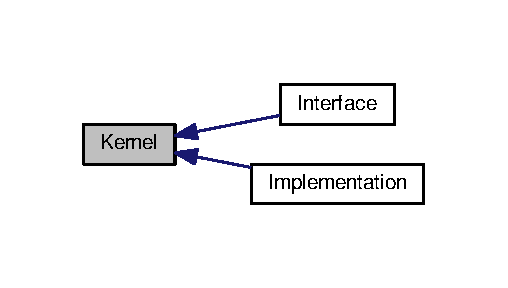
\includegraphics[width=244pt]{group__kern}
\end{center}
\end{figure}
\subsubsection*{Modules}
\begin{DoxyCompactItemize}
\item 
\hyperlink{group__kern__impl}{Implementation}
\begin{DoxyCompactList}\small\item\em Kernel port independent code implementation. \end{DoxyCompactList}\item 
\hyperlink{group__kern__intf}{Interface}
\begin{DoxyCompactList}\small\item\em Kernel main interface. \end{DoxyCompactList}\end{DoxyCompactItemize}


\subsubsection{Detailed Description}
Kernel overview. Main kernel interface is divided into several sections. 
\hypertarget{group__kern__intf}{\subsection{Interface}
\label{group__kern__intf}\index{Interface@{Interface}}
}


Application programming interface.  


Collaboration diagram for Interface\-:\nopagebreak
\begin{figure}[H]
\begin{center}
\leavevmode
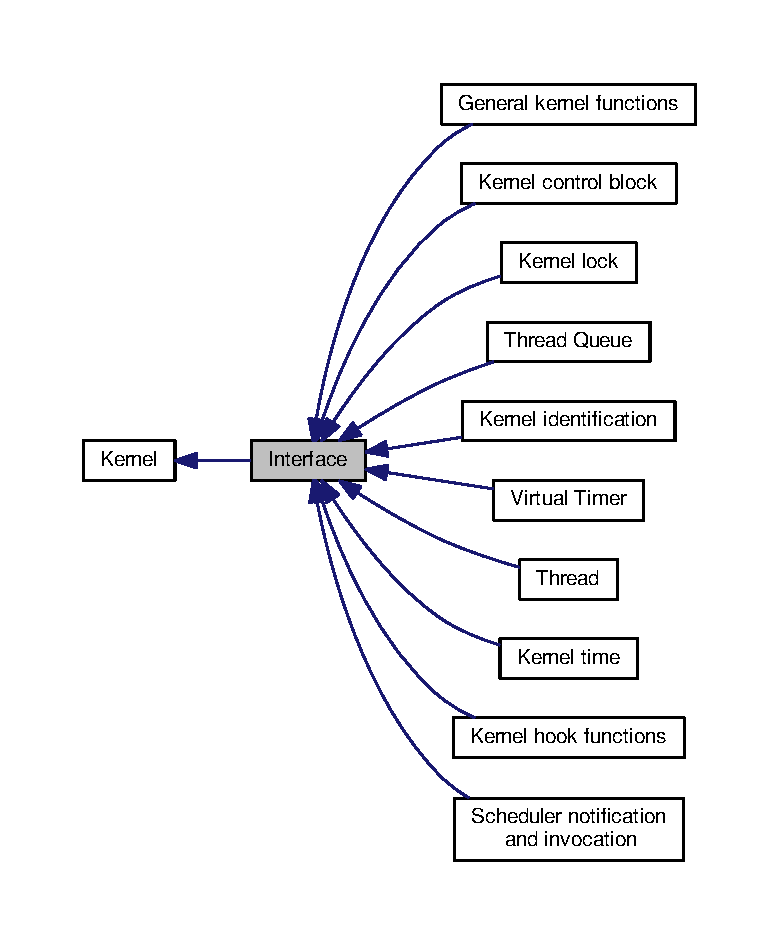
\includegraphics[width=216pt]{group__kern__intf}
\end{center}
\end{figure}
\subsubsection*{Data Structures}
\begin{DoxyCompactItemize}
\item 
struct \hyperlink{structesThd}{es\-Thd}
\begin{DoxyCompactList}\small\item\em Thread structure. \end{DoxyCompactList}\item 
struct \hyperlink{structesVTmr}{es\-V\-Tmr}
\begin{DoxyCompactList}\small\item\em Virtual Timer structure. \end{DoxyCompactList}\item 
struct \hyperlink{structesThdQ}{es\-Thd\-Q}
\begin{DoxyCompactList}\small\item\em Thread Queue structure. \end{DoxyCompactList}\item 
struct \hyperlink{structesKernCtrl}{es\-Kern\-Ctrl}
\begin{DoxyCompactList}\small\item\em Kernel control block structure. \end{DoxyCompactList}\end{DoxyCompactItemize}
\subsubsection*{Kernel identification and version number}
\begin{DoxyCompactItemize}
\item 
\#define \hyperlink{group__kern__intf_gacde22f7336a3c1c032dfc0ee3b94f506}{E\-S\-\_\-\-K\-E\-R\-N\-\_\-\-V\-E\-R}~0x10000ul
\begin{DoxyCompactList}\small\item\em Identifies the underlying kernel version number. \end{DoxyCompactList}\item 
\#define \hyperlink{group__kern__intf_ga7a9484c6b09349e4eb82ba67c0989e25}{E\-S\-\_\-\-K\-E\-R\-N\-\_\-\-I\-D}~\char`\"{}e\-Solid Kernel v1.\-0\char`\"{}
\begin{DoxyCompactList}\small\item\em Kernel identification string. \end{DoxyCompactList}\end{DoxyCompactItemize}
\subsubsection*{Critical section management}
\label{_amgrp43784aebc31664bf2b83e85766997ec9}%
These macros are used to prevent interrupts on entry into the critical section, and restoring interrupts to their previous state on exit from critical section.

For more details see \hyperlink{critical_section}{Critical sections}. \begin{DoxyCompactItemize}
\item 
\#define \hyperlink{group__kern__intf_ga0420d9c03ac590d6e3e46fd17f6a739e}{E\-S\-\_\-\-C\-R\-I\-T\-I\-C\-A\-L\-\_\-\-T}~P\-O\-R\-T\-\_\-\-C\-R\-I\-T\-I\-C\-A\-L\-\_\-\-T
\begin{DoxyCompactList}\small\item\em Critical section context variable type. \end{DoxyCompactList}\item 
\#define \hyperlink{group__kern__intf_ga90ec47263e8a05b91fe9359c97eb1c9c}{E\-S\-\_\-\-C\-R\-I\-T\-I\-C\-A\-L\-\_\-\-E\-N\-T\-E\-R}(ctx)~\hyperlink{group__template__cpu__intf_gad230b116bf8bc513e64c533d4e946054}{P\-O\-R\-T\-\_\-\-C\-R\-I\-T\-I\-C\-A\-L\-\_\-\-E\-N\-T\-E\-R}(ctx)
\begin{DoxyCompactList}\small\item\em Enter a critical section. \end{DoxyCompactList}\item 
\#define \hyperlink{group__kern__intf_gade4fcc55ee1325723ed798a8c5e11e56}{E\-S\-\_\-\-C\-R\-I\-T\-I\-C\-A\-L\-\_\-\-E\-X\-I\-T}(ctx)~\hyperlink{group__template__cpu__intf_ga95082ec189f12ed8e39efbda811dea77}{P\-O\-R\-T\-\_\-\-C\-R\-I\-T\-I\-C\-A\-L\-\_\-\-E\-X\-I\-T}(ctx)
\begin{DoxyCompactList}\small\item\em Exit from critical section. \end{DoxyCompactList}\item 
\#define \hyperlink{group__kern__intf_gacf1dc7063de829a77484e4c9e1e942a5}{E\-S\-\_\-\-C\-R\-I\-T\-I\-C\-A\-L\-\_\-\-E\-N\-T\-E\-R\-\_\-\-L\-O\-C\-K\-\_\-\-E\-X\-I\-T}()
\begin{DoxyCompactList}\small\item\em Enter critical section and exit scheduler lock. \end{DoxyCompactList}\item 
\#define \hyperlink{group__kern__intf_ga4466c8aea583e299815926cd4d262a2c}{E\-S\-\_\-\-C\-R\-I\-T\-I\-C\-A\-L\-\_\-\-E\-X\-I\-T\-\_\-\-L\-O\-C\-K\-\_\-\-E\-N\-T\-E\-R}()
\begin{DoxyCompactList}\small\item\em Exit critical section and enter scheduler lock. \end{DoxyCompactList}\end{DoxyCompactItemize}
\subsubsection*{Thread management}
\label{_amgrp46313fcfd6f520b7cdcbf505c023e3a2}%
Basic thread management services

For more details see \hyperlink{threads}{Thread Management}. \begin{DoxyCompactItemize}
\item 
typedef struct \hyperlink{structesThd}{es\-Thd} \hyperlink{group__kern__intf_ga62e3a3ca0a4597a19c43cb8868810d82}{es\-Thd\-\_\-\-T}
\begin{DoxyCompactList}\small\item\em Thread type. \end{DoxyCompactList}\item 
typedef \hyperlink{group__template__cpu__intf_ga13cc91970e3e05fe4210440c068d3f4a}{port\-Stck\-\_\-\-T} \hyperlink{group__kern__intf_ga24160ddd0cb0327108cc652bfe6a49e5}{es\-Stck\-\_\-\-T}
\begin{DoxyCompactList}\small\item\em Stack type. \end{DoxyCompactList}\item 
void \hyperlink{group__kern__intf_gac91734f3ee867b519f59bf81cc7fde88}{es\-Thd\-Init} (\hyperlink{group__kern__intf_ga62e3a3ca0a4597a19c43cb8868810d82}{es\-Thd\-\_\-\-T} $\ast$thd, void($\ast$fn)(void $\ast$), void $\ast$arg, \hyperlink{group__template__cpu__intf_ga13cc91970e3e05fe4210440c068d3f4a}{port\-Stck\-\_\-\-T} $\ast$stck, size\-\_\-t stck\-Size, uint8\-\_\-t prio)
\begin{DoxyCompactList}\small\item\em Initialize the specified thread. \end{DoxyCompactList}\item 
void \hyperlink{group__kern__intf_gac9d1eac76f26096614e8196bcfd8b905}{es\-Thd\-Term} (\hyperlink{group__kern__intf_ga62e3a3ca0a4597a19c43cb8868810d82}{es\-Thd\-\_\-\-T} $\ast$thd)
\begin{DoxyCompactList}\small\item\em Terminate the specified thread. \end{DoxyCompactList}\item 
static \hyperlink{group__template__compiler_ga87952d6e574c7f437503926e833ba345}{P\-O\-R\-T\-\_\-\-C\-\_\-\-I\-N\-L\-I\-N\-E} \hyperlink{group__kern__intf_ga62e3a3ca0a4597a19c43cb8868810d82}{es\-Thd\-\_\-\-T} $\ast$ \hyperlink{group__kern__intf_gae2a2c5fe0128d446a64512b0714bfb6d}{es\-Thd\-Get\-Id} (void)
\begin{DoxyCompactList}\small\item\em Get the current thread I\-D. \end{DoxyCompactList}\item 
static \hyperlink{group__template__compiler_ga87952d6e574c7f437503926e833ba345}{P\-O\-R\-T\-\_\-\-C\-\_\-\-I\-N\-L\-I\-N\-E} uint8\-\_\-t \hyperlink{group__kern__intf_ga6d2d033dc7e1226eccf4a51c666678ad}{es\-Thd\-Get\-Prio} (\hyperlink{group__kern__intf_ga62e3a3ca0a4597a19c43cb8868810d82}{es\-Thd\-\_\-\-T} $\ast$thd)
\begin{DoxyCompactList}\small\item\em Get the priority of a thread. \end{DoxyCompactList}\item 
void \hyperlink{group__kern__intf_ga8eaa731d0026a8a1667d4422d5031df6}{es\-Thd\-Set\-Prio\-I} (\hyperlink{group__kern__intf_ga62e3a3ca0a4597a19c43cb8868810d82}{es\-Thd\-\_\-\-T} $\ast$thd, uint8\-\_\-t prio)
\begin{DoxyCompactList}\small\item\em Set the priority of a thread. \end{DoxyCompactList}\item 
void \hyperlink{group__kern__intf_ga1c846f96eb842774a35fb1f8f720a229}{es\-Thd\-Post\-I} (\hyperlink{group__kern__intf_ga62e3a3ca0a4597a19c43cb8868810d82}{es\-Thd\-\_\-\-T} $\ast$thd)
\begin{DoxyCompactList}\small\item\em Post to thread semaphore. \end{DoxyCompactList}\item 
void \hyperlink{group__kern__intf_ga2505a886a7bc006061317a4924651e7c}{es\-Thd\-Post} (\hyperlink{group__kern__intf_ga62e3a3ca0a4597a19c43cb8868810d82}{es\-Thd\-\_\-\-T} $\ast$thd)
\begin{DoxyCompactList}\small\item\em Post to thread semaphore. \end{DoxyCompactList}\item 
void \hyperlink{group__kern__intf_ga6835afa8c355e01dc35a83310770a47c}{es\-Thd\-Wait\-I} (void)
\begin{DoxyCompactList}\small\item\em Wait for thread semaphore. \end{DoxyCompactList}\item 
void \hyperlink{group__kern__intf_gabbe4d89d1eba04a007fc39a9db6a5db9}{es\-Thd\-Wait} (void)
\begin{DoxyCompactList}\small\item\em Wait for thread semaphore. \end{DoxyCompactList}\item 
\#define \hyperlink{group__kern__intf_gaa707debebe3f98439911212b0cc8b3d1}{E\-S\-\_\-\-S\-T\-C\-K\-\_\-\-S\-I\-Z\-E}(elem)~\hyperlink{group__template__cpu__intf_gacb3a46e89d327fbaf5c122fe23877b24}{P\-O\-R\-T\-\_\-\-S\-T\-C\-K\-\_\-\-S\-I\-Z\-E}(elem)
\begin{DoxyCompactList}\small\item\em Converts the required stack elements into the stack array index. \end{DoxyCompactList}\item 
\hypertarget{group__kern__intf_gaea99f5a5153b96c419c384323a9e7bca}{\#define {\bfseries E\-S\-\_\-\-T\-H\-D\-\_\-\-P\-R\-I\-O\-\_\-\-M\-A\-X}~(\hyperlink{group__template__kern__cfg_ga56bd89fe76f7fe22f3d8805bc3c68892}{C\-F\-G\-\_\-\-S\-C\-H\-E\-D\-\_\-\-P\-R\-I\-O\-\_\-\-L\-V\-L} -\/ 2u)}\label{group__kern__intf_gaea99f5a5153b96c419c384323a9e7bca}

\item 
\hypertarget{group__kern__intf_gaec52780457f8ad9d4701b0d44a7ee0bc}{\#define {\bfseries E\-S\-\_\-\-T\-H\-D\-\_\-\-P\-R\-I\-O\-\_\-\-M\-I\-N}~(1u)}\label{group__kern__intf_gaec52780457f8ad9d4701b0d44a7ee0bc}

\end{DoxyCompactItemize}
\subsubsection*{Virtual Timer management}
\begin{DoxyCompactItemize}
\item 
typedef uint\-\_\-fast32\-\_\-t \hyperlink{group__kern__intf_ga844873888c186ee81eb66620dadb0451}{es\-Tick\-\_\-\-T}
\begin{DoxyCompactList}\small\item\em Timer tick type. \end{DoxyCompactList}\item 
typedef struct \hyperlink{structesVTmr}{es\-V\-Tmr} \hyperlink{group__kern__intf_ga3c020f0ca54ff412bc1d1505502d2afc}{es\-V\-Tmr\-\_\-\-T}
\begin{DoxyCompactList}\small\item\em Virtual Timer type. \end{DoxyCompactList}\item 
void \hyperlink{group__kern__intf_ga45fe650eac73e7fe203cc81565401555}{es\-V\-Tmr\-Init\-I} (\hyperlink{group__kern__intf_ga3c020f0ca54ff412bc1d1505502d2afc}{es\-V\-Tmr\-\_\-\-T} $\ast$v\-Tmr, \hyperlink{group__kern__intf_ga844873888c186ee81eb66620dadb0451}{es\-Tick\-\_\-\-T} tick, void($\ast$fn)(void $\ast$), void $\ast$arg)
\begin{DoxyCompactList}\small\item\em Add and start a new virtual timer. \end{DoxyCompactList}\item 
void \hyperlink{group__kern__intf_gad932cf00aec4ba03a0df02ccc493c4c2}{es\-V\-Tmr\-Init} (\hyperlink{group__kern__intf_ga3c020f0ca54ff412bc1d1505502d2afc}{es\-V\-Tmr\-\_\-\-T} $\ast$v\-Tmr, \hyperlink{group__kern__intf_ga844873888c186ee81eb66620dadb0451}{es\-Tick\-\_\-\-T} tick, void($\ast$fn)(void $\ast$), void $\ast$arg)
\begin{DoxyCompactList}\small\item\em Add and start a new virtual timer. \end{DoxyCompactList}\item 
void \hyperlink{group__kern__intf_ga96bb2c81f649c0305dfd08d1c79b2e37}{es\-V\-Tmr\-Term\-I} (\hyperlink{group__kern__intf_ga3c020f0ca54ff412bc1d1505502d2afc}{es\-V\-Tmr\-\_\-\-T} $\ast$v\-Tmr)
\begin{DoxyCompactList}\small\item\em Cancel and remove a virtual timer. \end{DoxyCompactList}\item 
void \hyperlink{group__kern__intf_gad6ec93a68e3526f18ed926cd441878cd}{es\-V\-Tmr\-Term} (\hyperlink{group__kern__intf_ga3c020f0ca54ff412bc1d1505502d2afc}{es\-V\-Tmr\-\_\-\-T} $\ast$v\-Tmr)
\begin{DoxyCompactList}\small\item\em Cancel and remove a virtual timer. \end{DoxyCompactList}\item 
void \hyperlink{group__kern__intf_ga26d10c6aaa0cd1d04261d2c9911e890d}{es\-V\-Tmr\-Delay} (\hyperlink{group__kern__intf_ga844873888c186ee81eb66620dadb0451}{es\-Tick\-\_\-\-T} tick)
\begin{DoxyCompactList}\small\item\em Delay for specified amount of ticks. \end{DoxyCompactList}\item 
\hypertarget{group__kern__intf_gacb0d88d6a7e467dc37a6a9a85945aaa6}{\hyperlink{group__kern__intf_ga844873888c186ee81eb66620dadb0451}{es\-Tick\-\_\-\-T} {\bfseries es\-Sys\-Tmr\-Tick\-Get} (void)}\label{group__kern__intf_gacb0d88d6a7e467dc37a6a9a85945aaa6}

\end{DoxyCompactItemize}
\subsubsection*{Thread Queue management}
\begin{DoxyCompactItemize}
\item 
typedef struct \hyperlink{structesThdQ}{es\-Thd\-Q} \hyperlink{group__kern__intf_ga7a1a060699e83a01512ebb5540019556}{es\-Thd\-Q\-\_\-\-T}
\begin{DoxyCompactList}\small\item\em Thread queue type. \end{DoxyCompactList}\item 
void \hyperlink{group__kern__intf_gaddd5fe0557c91559b9452beb0fc236fd}{es\-Thd\-Q\-Init} (\hyperlink{group__kern__intf_ga7a1a060699e83a01512ebb5540019556}{es\-Thd\-Q\-\_\-\-T} $\ast$thd\-Q)
\begin{DoxyCompactList}\small\item\em Initialize Thread Queue. \end{DoxyCompactList}\item 
void \hyperlink{group__kern__intf_gaa5f19b32a7f0c42616b5270dcbd73a3e}{es\-Thd\-Q\-Term} (\hyperlink{group__kern__intf_ga7a1a060699e83a01512ebb5540019556}{es\-Thd\-Q\-\_\-\-T} $\ast$thd\-Q)
\begin{DoxyCompactList}\small\item\em Terminate Thread Queue. \end{DoxyCompactList}\item 
void \hyperlink{group__kern__intf_ga9da1e71c137d8adb8c9bdead7052b5fa}{es\-Thd\-Q\-Add\-I} (\hyperlink{group__kern__intf_ga7a1a060699e83a01512ebb5540019556}{es\-Thd\-Q\-\_\-\-T} $\ast$thd\-Q, \hyperlink{group__kern__intf_ga62e3a3ca0a4597a19c43cb8868810d82}{es\-Thd\-\_\-\-T} $\ast$thd)
\begin{DoxyCompactList}\small\item\em Add a thread to the Thread Queue. \end{DoxyCompactList}\item 
void \hyperlink{group__kern__intf_gaa18afa95e34035da03c5cb7ea3a96320}{es\-Thd\-Q\-Rm\-I} (\hyperlink{group__kern__intf_ga7a1a060699e83a01512ebb5540019556}{es\-Thd\-Q\-\_\-\-T} $\ast$thd\-Q, \hyperlink{group__kern__intf_ga62e3a3ca0a4597a19c43cb8868810d82}{es\-Thd\-\_\-\-T} $\ast$thd)
\begin{DoxyCompactList}\small\item\em Removes the thread from the Thread Queue. \end{DoxyCompactList}\item 
\hyperlink{group__kern__intf_ga62e3a3ca0a4597a19c43cb8868810d82}{es\-Thd\-\_\-\-T} $\ast$ \hyperlink{group__kern__intf_ga1670c123f31c346b24ec9d2b7ae35f88}{es\-Thd\-Q\-Fetch\-I} (const \hyperlink{group__kern__intf_ga7a1a060699e83a01512ebb5540019556}{es\-Thd\-Q\-\_\-\-T} $\ast$thd\-Q)
\begin{DoxyCompactList}\small\item\em Fetch the first high priority thread from the Thread Queue. \end{DoxyCompactList}\item 
\hyperlink{group__kern__intf_ga62e3a3ca0a4597a19c43cb8868810d82}{es\-Thd\-\_\-\-T} $\ast$ \hyperlink{group__kern__intf_gae365b14292f1496a90d876baec84fb4e}{es\-Thd\-Q\-Fetch\-Rotate\-I} (\hyperlink{group__kern__intf_ga7a1a060699e83a01512ebb5540019556}{es\-Thd\-Q\-\_\-\-T} $\ast$thd\-Q, uint\-\_\-fast8\-\_\-t prio)
\begin{DoxyCompactList}\small\item\em Fetch the next thread and rotate thread linked list. \end{DoxyCompactList}\item 
\hyperlink{group__template__compiler_ga74fbee312f9185efb602f89d21b53404}{bool\-\_\-\-T} \hyperlink{group__kern__intf_gacf2687b82ce64e2154d97fd3b69a4ab5}{es\-Thd\-Q\-Is\-Empty} (const \hyperlink{group__kern__intf_ga7a1a060699e83a01512ebb5540019556}{es\-Thd\-Q\-\_\-\-T} $\ast$thd\-Q)
\begin{DoxyCompactList}\small\item\em Is thread queue empty. \end{DoxyCompactList}\item 
\#define \hyperlink{group__kern__intf_ga28fb55234bec595dbeb2c264ac084cc1}{P\-R\-I\-O\-\_\-\-B\-M\-\_\-\-G\-R\-P\-\_\-\-I\-N\-D\-X}~((\hyperlink{group__template__kern__cfg_ga56bd89fe76f7fe22f3d8805bc3c68892}{C\-F\-G\-\_\-\-S\-C\-H\-E\-D\-\_\-\-P\-R\-I\-O\-\_\-\-L\-V\-L} + P\-O\-R\-T\-\_\-\-D\-E\-F\-\_\-\-D\-A\-T\-A\-\_\-\-W\-I\-D\-T\-H -\/ 1u) / P\-O\-R\-T\-\_\-\-D\-E\-F\-\_\-\-D\-A\-T\-A\-\_\-\-W\-I\-D\-T\-H)
\begin{DoxyCompactList}\small\item\em Priority Bit Map Group Index. \end{DoxyCompactList}\end{DoxyCompactItemize}
\subsubsection*{Kernel control block}
\begin{DoxyCompactItemize}
\item 
enum \hyperlink{group__kern__intf_gac9be6bfeddbd6af148cdb3867fbc24af}{es\-Kern\-State} \{ \\*
\hyperlink{group__kern__intf_ggac9be6bfeddbd6af148cdb3867fbc24afa31a7e1ee10bcd82aaf8f5eca06ecdbe8}{E\-S\-\_\-\-K\-E\-R\-N\-\_\-\-R\-U\-N} = 0x00u, 
\\*
\hyperlink{group__kern__intf_ggac9be6bfeddbd6af148cdb3867fbc24afa62e34103bea61ea0b7a9816180a43905}{E\-S\-\_\-\-K\-E\-R\-N\-\_\-\-I\-N\-T\-S\-R\-V\-\_\-\-R\-U\-N} = 0x01u, 
\\*
\hyperlink{group__kern__intf_ggac9be6bfeddbd6af148cdb3867fbc24afa4e5b5c809ea9cdbae536b701003278cc}{E\-S\-\_\-\-K\-E\-R\-N\-\_\-\-L\-O\-C\-K} = 0x02u, 
\\*
\hyperlink{group__kern__intf_ggac9be6bfeddbd6af148cdb3867fbc24afa2b35c503975df4c289e9cbff3e815f8b}{E\-S\-\_\-\-K\-E\-R\-N\-\_\-\-I\-N\-T\-S\-R\-V\-\_\-\-L\-O\-C\-K} = 0x03u, 
\\*
\hyperlink{group__kern__intf_ggac9be6bfeddbd6af148cdb3867fbc24afad45a94c8b4975fd162d683201a75cceb}{E\-S\-\_\-\-K\-E\-R\-N\-\_\-\-S\-L\-E\-E\-P} = 0x06u, 
\\*
\hyperlink{group__kern__intf_ggac9be6bfeddbd6af148cdb3867fbc24afacad35dc43528f96d27696db584f05cff}{E\-S\-\_\-\-K\-E\-R\-N\-\_\-\-I\-N\-I\-T} = 0x08u, 
\\*
\hyperlink{group__kern__intf_ggac9be6bfeddbd6af148cdb3867fbc24afa089165cac55f315953335f5ffe41b7c4}{E\-S\-\_\-\-K\-E\-R\-N\-\_\-\-I\-N\-A\-C\-T\-I\-V\-E} = 0x10u
 \}
\begin{DoxyCompactList}\small\item\em Kernel state enumeration. \end{DoxyCompactList}\item 
typedef enum \hyperlink{group__kern__intf_gac9be6bfeddbd6af148cdb3867fbc24af}{es\-Kern\-State} \hyperlink{group__kern__intf_gab5edef44fe53303f96dc5e9f567babaf}{es\-Kern\-State\-\_\-\-T}
\begin{DoxyCompactList}\small\item\em Kernel state type. \end{DoxyCompactList}\item 
typedef struct \hyperlink{structesKernCtrl}{es\-Kern\-Ctrl} \hyperlink{group__kern__intf_gaae54a9918d92a2105b1d331b083d21b7}{es\-Kern\-Ctrl\-\_\-\-T}
\begin{DoxyCompactList}\small\item\em Kernel control block type. \end{DoxyCompactList}\item 
const volatile \hyperlink{group__kern__intf_gaae54a9918d92a2105b1d331b083d21b7}{es\-Kern\-Ctrl\-\_\-\-T} \hyperlink{group__kern__intf_ga299ac766f155bf1ef931627e2a0b895b}{g\-Kern\-Ctrl}
\begin{DoxyCompactList}\small\item\em Kernel control block. \end{DoxyCompactList}\end{DoxyCompactItemize}
\subsubsection*{General kernel functions}
\label{_amgrp41382adffec1bac51ecae38edaa569b6}%
There are several groups of functions\-:
\begin{DoxyItemize}
\item kernel initialization and start
\item I\-S\-R prologue and epilogue 
\end{DoxyItemize}\begin{DoxyCompactItemize}
\item 
void \hyperlink{group__kern__intf_ga9e9ff699d62d6035cd51121bb3140704}{es\-Kern\-Init} (void)
\begin{DoxyCompactList}\small\item\em Initialize kernel internal data structures. \end{DoxyCompactList}\item 
P\-O\-R\-T\-\_\-\-C\-\_\-\-N\-O\-R\-E\-T\-U\-R\-N void \hyperlink{group__kern__intf_ga0e7a0a6b9c02df58de0f98de0229a09d}{es\-Kern\-Start} (void)
\begin{DoxyCompactList}\small\item\em Start the multi-\/threading. \end{DoxyCompactList}\item 
void \hyperlink{group__kern__intf_ga3182e4c1a47897109d0a429b10a2483e}{es\-Kern\-Sys\-Tmr} (void)
\begin{DoxyCompactList}\small\item\em Process the system timer event. \end{DoxyCompactList}\item 
void \hyperlink{group__kern__intf_ga194f9cbc5398fe0938504a378fcff810}{es\-Kern\-Isr\-Prologue\-I} (void)
\begin{DoxyCompactList}\small\item\em Enter Interrupt Service Routine. \end{DoxyCompactList}\item 
void \hyperlink{group__kern__intf_ga62d9b43eb8faf6c5df37e7b89811ac8d}{es\-Kern\-Isr\-Epilogue\-I} (void)
\begin{DoxyCompactList}\small\item\em Exit Interrupt Service Routine. \end{DoxyCompactList}\end{DoxyCompactItemize}
\subsubsection*{Scheduler notification and invocation}
\begin{DoxyCompactItemize}
\item 
void \hyperlink{group__kern__intf_ga73e14b1860ce824c822adc407aee0977}{es\-Sched\-Rdy\-Add\-I} (\hyperlink{group__kern__intf_ga62e3a3ca0a4597a19c43cb8868810d82}{es\-Thd\-\_\-\-T} $\ast$thd)
\begin{DoxyCompactList}\small\item\em Add thread {\ttfamily thd} to the ready thread list and notify the scheduler. \end{DoxyCompactList}\item 
void \hyperlink{group__kern__intf_ga0b8263c5024ebb59cd9b95cc9253b44d}{es\-Sched\-Rdy\-Rm\-I} (\hyperlink{group__kern__intf_ga62e3a3ca0a4597a19c43cb8868810d82}{es\-Thd\-\_\-\-T} $\ast$thd)
\begin{DoxyCompactList}\small\item\em Remove thread {\ttfamily thd} from the ready thread list and notify the scheduler. \end{DoxyCompactList}\item 
void \hyperlink{group__kern__intf_gaf90e487bfce974dafaeed5009e189810}{es\-Sched\-Yield\-I} (void)
\begin{DoxyCompactList}\small\item\em Force the scheduler invocation which will evaluate all ready threads and switch to ready thread with the highest priority. \end{DoxyCompactList}\item 
void \hyperlink{group__kern__intf_gafbea29b376b29f11bbfc48a0f5144e9a}{es\-Sched\-Yield\-Isr\-I} (void)
\begin{DoxyCompactList}\small\item\em Force the scheduler invocation which will evaluate all ready threads and switch to ready thread with the highest priority. \end{DoxyCompactList}\item 
void \hyperlink{group__kern__intf_ga1e60d9df6ad1712ed57cd4ca038fcad2}{es\-Sched\-Lock\-Enter\-I} (void)
\begin{DoxyCompactList}\small\item\em Lock the scheduler. \end{DoxyCompactList}\item 
void \hyperlink{group__kern__intf_gaddd9b2fcbc03765f63f81b64e6663934}{es\-Sched\-Lock\-Exit\-I} (void)
\begin{DoxyCompactList}\small\item\em Unlock the scheduler. \end{DoxyCompactList}\item 
void \hyperlink{group__kern__intf_ga4b70a0e213b791b4e51840352d144a22}{es\-Sched\-Lock\-Enter} (void)
\begin{DoxyCompactList}\small\item\em Lock the scheduler. \end{DoxyCompactList}\item 
void \hyperlink{group__kern__intf_gac4c263203fcf700d96fe21782cfde219}{es\-Sched\-Lock\-Exit} (void)
\begin{DoxyCompactList}\small\item\em Unlock the scheduler. \end{DoxyCompactList}\end{DoxyCompactItemize}
\subsubsection*{Kernel hook functions}
\label{_amgrp1ac47bb3ac7873775afb0f49bf86f38e}%
\begin{DoxyNote}{Note}
1) The definition of this functions must be written by the user. 
\end{DoxyNote}
\begin{DoxyCompactItemize}
\item 
void \hyperlink{group__kern__intf_ga9a0d562969acef0121136b11be7b4728}{user\-Pre\-Sys\-Tmr} (void)
\begin{DoxyCompactList}\small\item\em System timer hook function, called from system system timer I\-S\-R function before the kernel functions. \end{DoxyCompactList}\item 
void \hyperlink{group__kern__intf_gaac77966856c9a299cda4794cbcc87edf}{user\-Pre\-Kern\-Init} (void)
\begin{DoxyCompactList}\small\item\em Kernel initialization hook function, called from \hyperlink{group__kern__intf_ga9e9ff699d62d6035cd51121bb3140704}{es\-Kern\-Init()} function before kernel initialization. \end{DoxyCompactList}\item 
void \hyperlink{group__kern__intf_ga3579ac6964a314ad03d13da0507f57e8}{user\-Post\-Kern\-Init} (void)
\begin{DoxyCompactList}\small\item\em Kernel initialization hook function, called from \hyperlink{group__kern__intf_ga9e9ff699d62d6035cd51121bb3140704}{es\-Kern\-Init()} function after kernel initialization. \end{DoxyCompactList}\item 
void \hyperlink{group__kern__intf_gaac505ab4c72e0fb346ca441d6def327d}{user\-Pre\-Kern\-Start} (void)
\begin{DoxyCompactList}\small\item\em Kernel start hook function, called from \hyperlink{group__kern__intf_ga0e7a0a6b9c02df58de0f98de0229a09d}{es\-Kern\-Start()} function. \end{DoxyCompactList}\item 
void \hyperlink{group__kern__intf_ga64ca864d0ff2aaa532208d7c2b88bdb3}{user\-Post\-Thd\-Init} (\hyperlink{group__kern__intf_ga62e3a3ca0a4597a19c43cb8868810d82}{es\-Thd\-\_\-\-T} $\ast$thd)
\begin{DoxyCompactList}\small\item\em Thread initialization end hook function, called from \hyperlink{group__kern__intf_gac91734f3ee867b519f59bf81cc7fde88}{es\-Thd\-Init()} function. \end{DoxyCompactList}\item 
void \hyperlink{group__kern__intf_ga076ad76633999c9d5e245e3b5c6e0c09}{user\-Pre\-Thd\-Term} (void)
\begin{DoxyCompactList}\small\item\em Thread terminate hook function, called from \hyperlink{group__kern__intf_gac9d1eac76f26096614e8196bcfd8b905}{es\-Thd\-Term()} or when a thread terminates itself. \end{DoxyCompactList}\item 
void \hyperlink{group__kern__intf_ga2bd40d82f768787c3dab2f4df336685e}{user\-Pre\-Idle} (void)
\begin{DoxyCompactList}\small\item\em Pre Idle hook function, called from idle thread, just before entering idle period. \end{DoxyCompactList}\item 
void \hyperlink{group__kern__intf_ga7ca4a96cbe5064d633298d1d172fd4e7}{user\-Post\-Idle} (void)
\begin{DoxyCompactList}\small\item\em Post idle hook function, called from idle thread, just after exiting idle period. \end{DoxyCompactList}\item 
void \hyperlink{group__kern__intf_ga74a38c965110d0f2f2e44e13571fe3fc}{user\-Pre\-Ctx\-Sw} (\hyperlink{group__kern__intf_ga62e3a3ca0a4597a19c43cb8868810d82}{es\-Thd\-\_\-\-T} $\ast$old\-Thd, \hyperlink{group__kern__intf_ga62e3a3ca0a4597a19c43cb8868810d82}{es\-Thd\-\_\-\-T} $\ast$new\-Thd)
\begin{DoxyCompactList}\small\item\em Kernel context switch hook function, called from \hyperlink{group__kern__intf_gaf90e487bfce974dafaeed5009e189810}{es\-Sched\-Yield\-I()} and \hyperlink{group__kern__intf_gafbea29b376b29f11bbfc48a0f5144e9a}{es\-Sched\-Yield\-Isr\-I()} functions just before context switch. \end{DoxyCompactList}\end{DoxyCompactItemize}


\subsubsection{Detailed Description}
Application programming interface. 

\subsubsection{Macro Definition Documentation}
\hypertarget{group__kern__intf_gacde22f7336a3c1c032dfc0ee3b94f506}{\index{Interface@{Interface}!E\-S\-\_\-\-K\-E\-R\-N\-\_\-\-V\-E\-R@{E\-S\-\_\-\-K\-E\-R\-N\-\_\-\-V\-E\-R}}
\index{E\-S\-\_\-\-K\-E\-R\-N\-\_\-\-V\-E\-R@{E\-S\-\_\-\-K\-E\-R\-N\-\_\-\-V\-E\-R}!Interface@{Interface}}
\paragraph[{E\-S\-\_\-\-K\-E\-R\-N\-\_\-\-V\-E\-R}]{\setlength{\rightskip}{0pt plus 5cm}\#define E\-S\-\_\-\-K\-E\-R\-N\-\_\-\-V\-E\-R~0x10000ul}}\label{group__kern__intf_gacde22f7336a3c1c032dfc0ee3b94f506}


Identifies the underlying kernel version number. 

Kernel identification and version (main \mbox{[}31\-:16\mbox{]} .sub \mbox{[}15\-:0\mbox{]}) \hypertarget{group__kern__intf_ga7a9484c6b09349e4eb82ba67c0989e25}{\index{Interface@{Interface}!E\-S\-\_\-\-K\-E\-R\-N\-\_\-\-I\-D@{E\-S\-\_\-\-K\-E\-R\-N\-\_\-\-I\-D}}
\index{E\-S\-\_\-\-K\-E\-R\-N\-\_\-\-I\-D@{E\-S\-\_\-\-K\-E\-R\-N\-\_\-\-I\-D}!Interface@{Interface}}
\paragraph[{E\-S\-\_\-\-K\-E\-R\-N\-\_\-\-I\-D}]{\setlength{\rightskip}{0pt plus 5cm}\#define E\-S\-\_\-\-K\-E\-R\-N\-\_\-\-I\-D~\char`\"{}e\-Solid Kernel v1.\-0\char`\"{}}}\label{group__kern__intf_ga7a9484c6b09349e4eb82ba67c0989e25}


Kernel identification string. 

\hypertarget{group__kern__intf_ga0420d9c03ac590d6e3e46fd17f6a739e}{\index{Interface@{Interface}!E\-S\-\_\-\-C\-R\-I\-T\-I\-C\-A\-L\-\_\-\-T@{E\-S\-\_\-\-C\-R\-I\-T\-I\-C\-A\-L\-\_\-\-T}}
\index{E\-S\-\_\-\-C\-R\-I\-T\-I\-C\-A\-L\-\_\-\-T@{E\-S\-\_\-\-C\-R\-I\-T\-I\-C\-A\-L\-\_\-\-T}!Interface@{Interface}}
\paragraph[{E\-S\-\_\-\-C\-R\-I\-T\-I\-C\-A\-L\-\_\-\-T}]{\setlength{\rightskip}{0pt plus 5cm}\#define E\-S\-\_\-\-C\-R\-I\-T\-I\-C\-A\-L\-\_\-\-T~P\-O\-R\-T\-\_\-\-C\-R\-I\-T\-I\-C\-A\-L\-\_\-\-T}}\label{group__kern__intf_ga0420d9c03ac590d6e3e46fd17f6a739e}


Critical section context variable type. 

\hypertarget{group__kern__intf_ga90ec47263e8a05b91fe9359c97eb1c9c}{\index{Interface@{Interface}!E\-S\-\_\-\-C\-R\-I\-T\-I\-C\-A\-L\-\_\-\-E\-N\-T\-E\-R@{E\-S\-\_\-\-C\-R\-I\-T\-I\-C\-A\-L\-\_\-\-E\-N\-T\-E\-R}}
\index{E\-S\-\_\-\-C\-R\-I\-T\-I\-C\-A\-L\-\_\-\-E\-N\-T\-E\-R@{E\-S\-\_\-\-C\-R\-I\-T\-I\-C\-A\-L\-\_\-\-E\-N\-T\-E\-R}!Interface@{Interface}}
\paragraph[{E\-S\-\_\-\-C\-R\-I\-T\-I\-C\-A\-L\-\_\-\-E\-N\-T\-E\-R}]{\setlength{\rightskip}{0pt plus 5cm}\#define E\-S\-\_\-\-C\-R\-I\-T\-I\-C\-A\-L\-\_\-\-E\-N\-T\-E\-R(
\begin{DoxyParamCaption}
\item[{}]{ctx}
\end{DoxyParamCaption}
)~{\bf P\-O\-R\-T\-\_\-\-C\-R\-I\-T\-I\-C\-A\-L\-\_\-\-E\-N\-T\-E\-R}(ctx)}}\label{group__kern__intf_ga90ec47263e8a05b91fe9359c97eb1c9c}


Enter a critical section. 

\hypertarget{group__kern__intf_gade4fcc55ee1325723ed798a8c5e11e56}{\index{Interface@{Interface}!E\-S\-\_\-\-C\-R\-I\-T\-I\-C\-A\-L\-\_\-\-E\-X\-I\-T@{E\-S\-\_\-\-C\-R\-I\-T\-I\-C\-A\-L\-\_\-\-E\-X\-I\-T}}
\index{E\-S\-\_\-\-C\-R\-I\-T\-I\-C\-A\-L\-\_\-\-E\-X\-I\-T@{E\-S\-\_\-\-C\-R\-I\-T\-I\-C\-A\-L\-\_\-\-E\-X\-I\-T}!Interface@{Interface}}
\paragraph[{E\-S\-\_\-\-C\-R\-I\-T\-I\-C\-A\-L\-\_\-\-E\-X\-I\-T}]{\setlength{\rightskip}{0pt plus 5cm}\#define E\-S\-\_\-\-C\-R\-I\-T\-I\-C\-A\-L\-\_\-\-E\-X\-I\-T(
\begin{DoxyParamCaption}
\item[{}]{ctx}
\end{DoxyParamCaption}
)~{\bf P\-O\-R\-T\-\_\-\-C\-R\-I\-T\-I\-C\-A\-L\-\_\-\-E\-X\-I\-T}(ctx)}}\label{group__kern__intf_gade4fcc55ee1325723ed798a8c5e11e56}


Exit from critical section. 

\hypertarget{group__kern__intf_gacf1dc7063de829a77484e4c9e1e942a5}{\index{Interface@{Interface}!E\-S\-\_\-\-C\-R\-I\-T\-I\-C\-A\-L\-\_\-\-E\-N\-T\-E\-R\-\_\-\-L\-O\-C\-K\-\_\-\-E\-X\-I\-T@{E\-S\-\_\-\-C\-R\-I\-T\-I\-C\-A\-L\-\_\-\-E\-N\-T\-E\-R\-\_\-\-L\-O\-C\-K\-\_\-\-E\-X\-I\-T}}
\index{E\-S\-\_\-\-C\-R\-I\-T\-I\-C\-A\-L\-\_\-\-E\-N\-T\-E\-R\-\_\-\-L\-O\-C\-K\-\_\-\-E\-X\-I\-T@{E\-S\-\_\-\-C\-R\-I\-T\-I\-C\-A\-L\-\_\-\-E\-N\-T\-E\-R\-\_\-\-L\-O\-C\-K\-\_\-\-E\-X\-I\-T}!Interface@{Interface}}
\paragraph[{E\-S\-\_\-\-C\-R\-I\-T\-I\-C\-A\-L\-\_\-\-E\-N\-T\-E\-R\-\_\-\-L\-O\-C\-K\-\_\-\-E\-X\-I\-T}]{\setlength{\rightskip}{0pt plus 5cm}\#define E\-S\-\_\-\-C\-R\-I\-T\-I\-C\-A\-L\-\_\-\-E\-N\-T\-E\-R\-\_\-\-L\-O\-C\-K\-\_\-\-E\-X\-I\-T(
\begin{DoxyParamCaption}
{}
\end{DoxyParamCaption}
)}}\label{group__kern__intf_gacf1dc7063de829a77484e4c9e1e942a5}
{\bfseries Value\-:}
\begin{DoxyCode}
\textcolor{keywordflow}{do} \{                                                                        \hyperlink{group__template__cpu__intf_gad230b116bf8bc513e64c533d4e946054}{\(\backslash\)}
\hyperlink{group__template__cpu__intf_gad230b116bf8bc513e64c533d4e946054}{        PORT\_CRITICAL\_ENTER}();                                                  
      \hyperlink{group__kern__intf_gaddd9b2fcbc03765f63f81b64e6663934}{\(\backslash\)}
\hyperlink{group__kern__intf_gaddd9b2fcbc03765f63f81b64e6663934}{        esSchedLockExitI}();                                                     \(\backslash\)
    \} \textcolor{keywordflow}{while} (0U)
\end{DoxyCode}


Enter critical section and exit scheduler lock. 

\hypertarget{group__kern__intf_ga4466c8aea583e299815926cd4d262a2c}{\index{Interface@{Interface}!E\-S\-\_\-\-C\-R\-I\-T\-I\-C\-A\-L\-\_\-\-E\-X\-I\-T\-\_\-\-L\-O\-C\-K\-\_\-\-E\-N\-T\-E\-R@{E\-S\-\_\-\-C\-R\-I\-T\-I\-C\-A\-L\-\_\-\-E\-X\-I\-T\-\_\-\-L\-O\-C\-K\-\_\-\-E\-N\-T\-E\-R}}
\index{E\-S\-\_\-\-C\-R\-I\-T\-I\-C\-A\-L\-\_\-\-E\-X\-I\-T\-\_\-\-L\-O\-C\-K\-\_\-\-E\-N\-T\-E\-R@{E\-S\-\_\-\-C\-R\-I\-T\-I\-C\-A\-L\-\_\-\-E\-X\-I\-T\-\_\-\-L\-O\-C\-K\-\_\-\-E\-N\-T\-E\-R}!Interface@{Interface}}
\paragraph[{E\-S\-\_\-\-C\-R\-I\-T\-I\-C\-A\-L\-\_\-\-E\-X\-I\-T\-\_\-\-L\-O\-C\-K\-\_\-\-E\-N\-T\-E\-R}]{\setlength{\rightskip}{0pt plus 5cm}\#define E\-S\-\_\-\-C\-R\-I\-T\-I\-C\-A\-L\-\_\-\-E\-X\-I\-T\-\_\-\-L\-O\-C\-K\-\_\-\-E\-N\-T\-E\-R(
\begin{DoxyParamCaption}
{}
\end{DoxyParamCaption}
)}}\label{group__kern__intf_ga4466c8aea583e299815926cd4d262a2c}
{\bfseries Value\-:}
\begin{DoxyCode}
\textcolor{keywordflow}{do} \{                                                                        \hyperlink{group__kern__intf_ga1e60d9df6ad1712ed57cd4ca038fcad2}{\(\backslash\)}
\hyperlink{group__kern__intf_ga1e60d9df6ad1712ed57cd4ca038fcad2}{        esSchedLockEnterI}();                                                    
      \hyperlink{group__template__cpu__intf_ga95082ec189f12ed8e39efbda811dea77}{\(\backslash\)}
\hyperlink{group__template__cpu__intf_ga95082ec189f12ed8e39efbda811dea77}{        PORT\_CRITICAL\_EXIT}();                                                   \(\backslash\)
    \} \textcolor{keywordflow}{while} (0U)
\end{DoxyCode}


Exit critical section and enter scheduler lock. 

\hypertarget{group__kern__intf_gaa707debebe3f98439911212b0cc8b3d1}{\index{Interface@{Interface}!E\-S\-\_\-\-S\-T\-C\-K\-\_\-\-S\-I\-Z\-E@{E\-S\-\_\-\-S\-T\-C\-K\-\_\-\-S\-I\-Z\-E}}
\index{E\-S\-\_\-\-S\-T\-C\-K\-\_\-\-S\-I\-Z\-E@{E\-S\-\_\-\-S\-T\-C\-K\-\_\-\-S\-I\-Z\-E}!Interface@{Interface}}
\paragraph[{E\-S\-\_\-\-S\-T\-C\-K\-\_\-\-S\-I\-Z\-E}]{\setlength{\rightskip}{0pt plus 5cm}\#define E\-S\-\_\-\-S\-T\-C\-K\-\_\-\-S\-I\-Z\-E(
\begin{DoxyParamCaption}
\item[{}]{elem}
\end{DoxyParamCaption}
)~{\bf P\-O\-R\-T\-\_\-\-S\-T\-C\-K\-\_\-\-S\-I\-Z\-E}(elem)}}\label{group__kern__intf_gaa707debebe3f98439911212b0cc8b3d1}


Converts the required stack elements into the stack array index. 


\begin{DoxyParams}{Parameters}
{\em elem} & Number of stack elements\-: the stack size is expressed in number of elements regardles of the size of port general purpose registers. \\
\hline
\end{DoxyParams}
\hypertarget{group__kern__intf_ga28fb55234bec595dbeb2c264ac084cc1}{\index{Interface@{Interface}!P\-R\-I\-O\-\_\-\-B\-M\-\_\-\-G\-R\-P\-\_\-\-I\-N\-D\-X@{P\-R\-I\-O\-\_\-\-B\-M\-\_\-\-G\-R\-P\-\_\-\-I\-N\-D\-X}}
\index{P\-R\-I\-O\-\_\-\-B\-M\-\_\-\-G\-R\-P\-\_\-\-I\-N\-D\-X@{P\-R\-I\-O\-\_\-\-B\-M\-\_\-\-G\-R\-P\-\_\-\-I\-N\-D\-X}!Interface@{Interface}}
\paragraph[{P\-R\-I\-O\-\_\-\-B\-M\-\_\-\-G\-R\-P\-\_\-\-I\-N\-D\-X}]{\setlength{\rightskip}{0pt plus 5cm}\#define P\-R\-I\-O\-\_\-\-B\-M\-\_\-\-G\-R\-P\-\_\-\-I\-N\-D\-X~(({\bf C\-F\-G\-\_\-\-S\-C\-H\-E\-D\-\_\-\-P\-R\-I\-O\-\_\-\-L\-V\-L} + P\-O\-R\-T\-\_\-\-D\-E\-F\-\_\-\-D\-A\-T\-A\-\_\-\-W\-I\-D\-T\-H -\/ 1u) / P\-O\-R\-T\-\_\-\-D\-E\-F\-\_\-\-D\-A\-T\-A\-\_\-\-W\-I\-D\-T\-H)}}\label{group__kern__intf_ga28fb55234bec595dbeb2c264ac084cc1}


Priority Bit Map Group Index. 

\begin{DoxyParagraph}{Object class\-:}
{\bfseries Not A\-P\-I} object, this object is not part of the application programming interface and it is intended for internal use only. 
\end{DoxyParagraph}


\subsubsection{Typedef Documentation}
\hypertarget{group__kern__intf_ga62e3a3ca0a4597a19c43cb8868810d82}{\index{Interface@{Interface}!es\-Thd\-\_\-\-T@{es\-Thd\-\_\-\-T}}
\index{es\-Thd\-\_\-\-T@{es\-Thd\-\_\-\-T}!Interface@{Interface}}
\paragraph[{es\-Thd\-\_\-\-T}]{\setlength{\rightskip}{0pt plus 5cm}typedef struct {\bf es\-Thd} {\bf es\-Thd\-\_\-\-T}}}\label{group__kern__intf_ga62e3a3ca0a4597a19c43cb8868810d82}


Thread type. 

\hypertarget{group__kern__intf_ga24160ddd0cb0327108cc652bfe6a49e5}{\index{Interface@{Interface}!es\-Stck\-\_\-\-T@{es\-Stck\-\_\-\-T}}
\index{es\-Stck\-\_\-\-T@{es\-Stck\-\_\-\-T}!Interface@{Interface}}
\paragraph[{es\-Stck\-\_\-\-T}]{\setlength{\rightskip}{0pt plus 5cm}typedef {\bf port\-Stck\-\_\-\-T} {\bf es\-Stck\-\_\-\-T}}}\label{group__kern__intf_ga24160ddd0cb0327108cc652bfe6a49e5}


Stack type. 

\hypertarget{group__kern__intf_ga844873888c186ee81eb66620dadb0451}{\index{Interface@{Interface}!es\-Tick\-\_\-\-T@{es\-Tick\-\_\-\-T}}
\index{es\-Tick\-\_\-\-T@{es\-Tick\-\_\-\-T}!Interface@{Interface}}
\paragraph[{es\-Tick\-\_\-\-T}]{\setlength{\rightskip}{0pt plus 5cm}typedef uint\-\_\-fast32\-\_\-t {\bf es\-Tick\-\_\-\-T}}}\label{group__kern__intf_ga844873888c186ee81eb66620dadb0451}


Timer tick type. 

\hypertarget{group__kern__intf_ga3c020f0ca54ff412bc1d1505502d2afc}{\index{Interface@{Interface}!es\-V\-Tmr\-\_\-\-T@{es\-V\-Tmr\-\_\-\-T}}
\index{es\-V\-Tmr\-\_\-\-T@{es\-V\-Tmr\-\_\-\-T}!Interface@{Interface}}
\paragraph[{es\-V\-Tmr\-\_\-\-T}]{\setlength{\rightskip}{0pt plus 5cm}typedef struct {\bf es\-V\-Tmr} {\bf es\-V\-Tmr\-\_\-\-T}}}\label{group__kern__intf_ga3c020f0ca54ff412bc1d1505502d2afc}


Virtual Timer type. 

\hypertarget{group__kern__intf_ga7a1a060699e83a01512ebb5540019556}{\index{Interface@{Interface}!es\-Thd\-Q\-\_\-\-T@{es\-Thd\-Q\-\_\-\-T}}
\index{es\-Thd\-Q\-\_\-\-T@{es\-Thd\-Q\-\_\-\-T}!Interface@{Interface}}
\paragraph[{es\-Thd\-Q\-\_\-\-T}]{\setlength{\rightskip}{0pt plus 5cm}typedef struct {\bf es\-Thd\-Q} {\bf es\-Thd\-Q\-\_\-\-T}}}\label{group__kern__intf_ga7a1a060699e83a01512ebb5540019556}


Thread queue type. 

\hypertarget{group__kern__intf_gab5edef44fe53303f96dc5e9f567babaf}{\index{Interface@{Interface}!es\-Kern\-State\-\_\-\-T@{es\-Kern\-State\-\_\-\-T}}
\index{es\-Kern\-State\-\_\-\-T@{es\-Kern\-State\-\_\-\-T}!Interface@{Interface}}
\paragraph[{es\-Kern\-State\-\_\-\-T}]{\setlength{\rightskip}{0pt plus 5cm}typedef enum {\bf es\-Kern\-State} {\bf es\-Kern\-State\-\_\-\-T}}}\label{group__kern__intf_gab5edef44fe53303f96dc5e9f567babaf}


Kernel state type. 

\hypertarget{group__kern__intf_gaae54a9918d92a2105b1d331b083d21b7}{\index{Interface@{Interface}!es\-Kern\-Ctrl\-\_\-\-T@{es\-Kern\-Ctrl\-\_\-\-T}}
\index{es\-Kern\-Ctrl\-\_\-\-T@{es\-Kern\-Ctrl\-\_\-\-T}!Interface@{Interface}}
\paragraph[{es\-Kern\-Ctrl\-\_\-\-T}]{\setlength{\rightskip}{0pt plus 5cm}typedef struct {\bf es\-Kern\-Ctrl} {\bf es\-Kern\-Ctrl\-\_\-\-T}}}\label{group__kern__intf_gaae54a9918d92a2105b1d331b083d21b7}


Kernel control block type. 



\subsubsection{Enumeration Type Documentation}
\hypertarget{group__kern__intf_gac9be6bfeddbd6af148cdb3867fbc24af}{\index{Interface@{Interface}!es\-Kern\-State@{es\-Kern\-State}}
\index{es\-Kern\-State@{es\-Kern\-State}!Interface@{Interface}}
\paragraph[{es\-Kern\-State}]{\setlength{\rightskip}{0pt plus 5cm}enum {\bf es\-Kern\-State}}}\label{group__kern__intf_gac9be6bfeddbd6af148cdb3867fbc24af}


Kernel state enumeration. 

For more details see\-: \hyperlink{states}{Kernel states} \begin{DoxyParagraph}{Object class\-:}
Regular {\bfseries A\-P\-I} object, this object is part of the application programming interface. 
\end{DoxyParagraph}
\begin{Desc}
\item[Enumerator]\par
\begin{description}
\index{E\-S\-\_\-\-K\-E\-R\-N\-\_\-\-R\-U\-N@{E\-S\-\_\-\-K\-E\-R\-N\-\_\-\-R\-U\-N}!Interface@{Interface}}\index{Interface@{Interface}!E\-S\-\_\-\-K\-E\-R\-N\-\_\-\-R\-U\-N@{E\-S\-\_\-\-K\-E\-R\-N\-\_\-\-R\-U\-N}}\item[{\em 
\hypertarget{group__kern__intf_ggac9be6bfeddbd6af148cdb3867fbc24afa31a7e1ee10bcd82aaf8f5eca06ecdbe8}{E\-S\-\_\-\-K\-E\-R\-N\-\_\-\-R\-U\-N}\label{group__kern__intf_ggac9be6bfeddbd6af148cdb3867fbc24afa31a7e1ee10bcd82aaf8f5eca06ecdbe8}
}]Kernel is active \index{E\-S\-\_\-\-K\-E\-R\-N\-\_\-\-I\-N\-T\-S\-R\-V\-\_\-\-R\-U\-N@{E\-S\-\_\-\-K\-E\-R\-N\-\_\-\-I\-N\-T\-S\-R\-V\-\_\-\-R\-U\-N}!Interface@{Interface}}\index{Interface@{Interface}!E\-S\-\_\-\-K\-E\-R\-N\-\_\-\-I\-N\-T\-S\-R\-V\-\_\-\-R\-U\-N@{E\-S\-\_\-\-K\-E\-R\-N\-\_\-\-I\-N\-T\-S\-R\-V\-\_\-\-R\-U\-N}}\item[{\em 
\hypertarget{group__kern__intf_ggac9be6bfeddbd6af148cdb3867fbc24afa62e34103bea61ea0b7a9816180a43905}{E\-S\-\_\-\-K\-E\-R\-N\-\_\-\-I\-N\-T\-S\-R\-V\-\_\-\-R\-U\-N}\label{group__kern__intf_ggac9be6bfeddbd6af148cdb3867fbc24afa62e34103bea61ea0b7a9816180a43905}
}]Servicing an interrupt return to E\-S\-\_\-\-K\-E\-R\-N\-\_\-\-R\-U\-N state \index{E\-S\-\_\-\-K\-E\-R\-N\-\_\-\-L\-O\-C\-K@{E\-S\-\_\-\-K\-E\-R\-N\-\_\-\-L\-O\-C\-K}!Interface@{Interface}}\index{Interface@{Interface}!E\-S\-\_\-\-K\-E\-R\-N\-\_\-\-L\-O\-C\-K@{E\-S\-\_\-\-K\-E\-R\-N\-\_\-\-L\-O\-C\-K}}\item[{\em 
\hypertarget{group__kern__intf_ggac9be6bfeddbd6af148cdb3867fbc24afa4e5b5c809ea9cdbae536b701003278cc}{E\-S\-\_\-\-K\-E\-R\-N\-\_\-\-L\-O\-C\-K}\label{group__kern__intf_ggac9be6bfeddbd6af148cdb3867fbc24afa4e5b5c809ea9cdbae536b701003278cc}
}]Kernel is locked \index{E\-S\-\_\-\-K\-E\-R\-N\-\_\-\-I\-N\-T\-S\-R\-V\-\_\-\-L\-O\-C\-K@{E\-S\-\_\-\-K\-E\-R\-N\-\_\-\-I\-N\-T\-S\-R\-V\-\_\-\-L\-O\-C\-K}!Interface@{Interface}}\index{Interface@{Interface}!E\-S\-\_\-\-K\-E\-R\-N\-\_\-\-I\-N\-T\-S\-R\-V\-\_\-\-L\-O\-C\-K@{E\-S\-\_\-\-K\-E\-R\-N\-\_\-\-I\-N\-T\-S\-R\-V\-\_\-\-L\-O\-C\-K}}\item[{\em 
\hypertarget{group__kern__intf_ggac9be6bfeddbd6af148cdb3867fbc24afa2b35c503975df4c289e9cbff3e815f8b}{E\-S\-\_\-\-K\-E\-R\-N\-\_\-\-I\-N\-T\-S\-R\-V\-\_\-\-L\-O\-C\-K}\label{group__kern__intf_ggac9be6bfeddbd6af148cdb3867fbc24afa2b35c503975df4c289e9cbff3e815f8b}
}]Servicing an interrupt, return to E\-S\-\_\-\-K\-E\-R\-N\-\_\-\-L\-O\-C\-K state \index{E\-S\-\_\-\-K\-E\-R\-N\-\_\-\-S\-L\-E\-E\-P@{E\-S\-\_\-\-K\-E\-R\-N\-\_\-\-S\-L\-E\-E\-P}!Interface@{Interface}}\index{Interface@{Interface}!E\-S\-\_\-\-K\-E\-R\-N\-\_\-\-S\-L\-E\-E\-P@{E\-S\-\_\-\-K\-E\-R\-N\-\_\-\-S\-L\-E\-E\-P}}\item[{\em 
\hypertarget{group__kern__intf_ggac9be6bfeddbd6af148cdb3867fbc24afad45a94c8b4975fd162d683201a75cceb}{E\-S\-\_\-\-K\-E\-R\-N\-\_\-\-S\-L\-E\-E\-P}\label{group__kern__intf_ggac9be6bfeddbd6af148cdb3867fbc24afad45a94c8b4975fd162d683201a75cceb}
}]Kernel is sleeping \index{E\-S\-\_\-\-K\-E\-R\-N\-\_\-\-I\-N\-I\-T@{E\-S\-\_\-\-K\-E\-R\-N\-\_\-\-I\-N\-I\-T}!Interface@{Interface}}\index{Interface@{Interface}!E\-S\-\_\-\-K\-E\-R\-N\-\_\-\-I\-N\-I\-T@{E\-S\-\_\-\-K\-E\-R\-N\-\_\-\-I\-N\-I\-T}}\item[{\em 
\hypertarget{group__kern__intf_ggac9be6bfeddbd6af148cdb3867fbc24afacad35dc43528f96d27696db584f05cff}{E\-S\-\_\-\-K\-E\-R\-N\-\_\-\-I\-N\-I\-T}\label{group__kern__intf_ggac9be6bfeddbd6af148cdb3867fbc24afacad35dc43528f96d27696db584f05cff}
}]Kernel is in initialization state \index{E\-S\-\_\-\-K\-E\-R\-N\-\_\-\-I\-N\-A\-C\-T\-I\-V\-E@{E\-S\-\_\-\-K\-E\-R\-N\-\_\-\-I\-N\-A\-C\-T\-I\-V\-E}!Interface@{Interface}}\index{Interface@{Interface}!E\-S\-\_\-\-K\-E\-R\-N\-\_\-\-I\-N\-A\-C\-T\-I\-V\-E@{E\-S\-\_\-\-K\-E\-R\-N\-\_\-\-I\-N\-A\-C\-T\-I\-V\-E}}\item[{\em 
\hypertarget{group__kern__intf_ggac9be6bfeddbd6af148cdb3867fbc24afa089165cac55f315953335f5ffe41b7c4}{E\-S\-\_\-\-K\-E\-R\-N\-\_\-\-I\-N\-A\-C\-T\-I\-V\-E}\label{group__kern__intf_ggac9be6bfeddbd6af148cdb3867fbc24afa089165cac55f315953335f5ffe41b7c4}
}]Kernel data structures are not initialized \end{description}
\end{Desc}


\subsubsection{Function Documentation}
\hypertarget{group__kern__intf_ga9e9ff699d62d6035cd51121bb3140704}{\index{Interface@{Interface}!es\-Kern\-Init@{es\-Kern\-Init}}
\index{es\-Kern\-Init@{es\-Kern\-Init}!Interface@{Interface}}
\paragraph[{es\-Kern\-Init}]{\setlength{\rightskip}{0pt plus 5cm}void es\-Kern\-Init (
\begin{DoxyParamCaption}
\item[{void}]{}
\end{DoxyParamCaption}
)}}\label{group__kern__intf_ga9e9ff699d62d6035cd51121bb3140704}


Initialize kernel internal data structures. 

\begin{DoxyPrecond}{Precondition}
1) {\ttfamily The kernel state == E\-S\-\_\-\-K\-E\-R\-N\-\_\-\-I\-N\-A\-C\-T\-I\-V\-E}, see \hyperlink{states}{Kernel states}. 
\end{DoxyPrecond}
\begin{DoxyPostcond}{Postcondition}
1) {\ttfamily The kernel state == E\-S\-\_\-\-K\-E\-R\-N\-\_\-\-I\-N\-I\-T}. 
\end{DoxyPostcond}
\begin{DoxyNote}{Note}
1) This function may be invoked only once.
\end{DoxyNote}
This function must be called first before any other kernel A\-P\-I. It initializes internal data structures that are used by other A\-P\-I functions. \begin{DoxyParagraph}{This service can be called from\-:}

\begin{DoxyItemize}
\item Application initialization code 
\end{DoxyItemize}
\end{DoxyParagraph}
\begin{DoxyParagraph}{Rescheduling\-:}

\begin{DoxyItemize}
\item never 
\end{DoxyItemize}
\end{DoxyParagraph}
\begin{DoxyParagraph}{Object class\-:}
Regular {\bfseries A\-P\-I} object, this object is part of the application programming interface. 
\end{DoxyParagraph}
\hypertarget{group__kern__intf_ga0e7a0a6b9c02df58de0f98de0229a09d}{\index{Interface@{Interface}!es\-Kern\-Start@{es\-Kern\-Start}}
\index{es\-Kern\-Start@{es\-Kern\-Start}!Interface@{Interface}}
\paragraph[{es\-Kern\-Start}]{\setlength{\rightskip}{0pt plus 5cm}P\-O\-R\-T\-\_\-\-C\-\_\-\-N\-O\-R\-E\-T\-U\-R\-N void es\-Kern\-Start (
\begin{DoxyParamCaption}
\item[{void}]{}
\end{DoxyParamCaption}
)}}\label{group__kern__intf_ga0e7a0a6b9c02df58de0f98de0229a09d}


Start the multi-\/threading. 

\begin{DoxyPrecond}{Precondition}
1) {\ttfamily The kernel state == E\-S\-\_\-\-K\-E\-R\-N\-\_\-\-I\-N\-I\-T}, see \hyperlink{states}{Kernel states}. 
\end{DoxyPrecond}
\begin{DoxyPostcond}{Postcondition}
1) {\ttfamily The kernel state == E\-S\-\_\-\-K\-E\-R\-N\-\_\-\-R\-U\-N} 

2) The multi-\/threading execution will commence. 
\end{DoxyPostcond}
\begin{DoxyNote}{Note}
1) Once this function is called the execution of threads will start and this function will never return.
\end{DoxyNote}
This function will start multi-\/threading. Once the multi-\/threading has started the execution will never return to this function again (this function never returns). \begin{DoxyParagraph}{This service can be called from\-:}

\begin{DoxyItemize}
\item Application initialization code 
\end{DoxyItemize}
\end{DoxyParagraph}
\begin{DoxyParagraph}{Rescheduling\-:}

\begin{DoxyItemize}
\item always 
\end{DoxyItemize}
\end{DoxyParagraph}
\begin{DoxyParagraph}{Object class\-:}
Regular {\bfseries A\-P\-I} object, this object is part of the application programming interface. 
\end{DoxyParagraph}
\hypertarget{group__kern__intf_ga3182e4c1a47897109d0a429b10a2483e}{\index{Interface@{Interface}!es\-Kern\-Sys\-Tmr@{es\-Kern\-Sys\-Tmr}}
\index{es\-Kern\-Sys\-Tmr@{es\-Kern\-Sys\-Tmr}!Interface@{Interface}}
\paragraph[{es\-Kern\-Sys\-Tmr}]{\setlength{\rightskip}{0pt plus 5cm}void es\-Kern\-Sys\-Tmr (
\begin{DoxyParamCaption}
\item[{void}]{}
\end{DoxyParamCaption}
)}}\label{group__kern__intf_ga3182e4c1a47897109d0a429b10a2483e}


Process the system timer event. 

\begin{DoxyPrecond}{Precondition}
1) {\ttfamily The kernel state $<$ E\-S\-\_\-\-K\-E\-R\-N\-\_\-\-I\-N\-I\-T}, see \hyperlink{states}{Kernel states}.
\end{DoxyPrecond}
This function will be called only by port system timer interrupt. \begin{DoxyParagraph}{Object class\-:}
{\bfseries Not A\-P\-I} object, this object is not part of the application programming interface and it is intended for internal use only. 
\end{DoxyParagraph}
\hypertarget{group__kern__intf_ga194f9cbc5398fe0938504a378fcff810}{\index{Interface@{Interface}!es\-Kern\-Isr\-Prologue\-I@{es\-Kern\-Isr\-Prologue\-I}}
\index{es\-Kern\-Isr\-Prologue\-I@{es\-Kern\-Isr\-Prologue\-I}!Interface@{Interface}}
\paragraph[{es\-Kern\-Isr\-Prologue\-I}]{\setlength{\rightskip}{0pt plus 5cm}void es\-Kern\-Isr\-Prologue\-I (
\begin{DoxyParamCaption}
\item[{void}]{}
\end{DoxyParamCaption}
)}}\label{group__kern__intf_ga194f9cbc5398fe0938504a378fcff810}


Enter Interrupt Service Routine. 

\begin{DoxyPrecond}{Precondition}
1) {\ttfamily The kernel state $<$ E\-S\-\_\-\-K\-E\-R\-N\-\_\-\-I\-N\-I\-T}, see \hyperlink{states}{Kernel states}. 
\end{DoxyPrecond}
\begin{DoxyNote}{Note}
1) You must call \hyperlink{group__kern__intf_ga62d9b43eb8faf6c5df37e7b89811ac8d}{es\-Kern\-Isr\-Epilogue\-I()} at the exit of I\-S\-R. 

2) You must invoke \hyperlink{group__kern__intf_ga194f9cbc5398fe0938504a378fcff810}{es\-Kern\-Isr\-Prologue\-I()} and \hyperlink{group__kern__intf_ga62d9b43eb8faf6c5df37e7b89811ac8d}{es\-Kern\-Isr\-Epilogue\-I()} in pair. In other words, for every call to \hyperlink{group__kern__intf_ga194f9cbc5398fe0938504a378fcff810}{es\-Kern\-Isr\-Prologue\-I()} at the beginning of the I\-S\-R you must have a call to \hyperlink{group__kern__intf_ga62d9b43eb8faf6c5df37e7b89811ac8d}{es\-Kern\-Isr\-Epilogue\-I()} at the end of the I\-S\-R.
\end{DoxyNote}
Function will notify kernel that you are about to enter interrupt service routine (I\-S\-R). This allows kernel to keep track of interrupt nesting and then only perform rescheduling at the last nested I\-S\-R. \begin{DoxyParagraph}{This service can be called from\-:}

\begin{DoxyItemize}
\item Interrupt service routine 
\end{DoxyItemize}
\end{DoxyParagraph}
\begin{DoxyParagraph}{Rescheduling\-:}

\begin{DoxyItemize}
\item never 
\end{DoxyItemize}
\end{DoxyParagraph}
\begin{DoxyParagraph}{Function class\-:}
{\bfseries I class}, Interrupt-\/lock A\-P\-I function, this function can be called only from interrupts locked code sections. 
\end{DoxyParagraph}
\hypertarget{group__kern__intf_ga62d9b43eb8faf6c5df37e7b89811ac8d}{\index{Interface@{Interface}!es\-Kern\-Isr\-Epilogue\-I@{es\-Kern\-Isr\-Epilogue\-I}}
\index{es\-Kern\-Isr\-Epilogue\-I@{es\-Kern\-Isr\-Epilogue\-I}!Interface@{Interface}}
\paragraph[{es\-Kern\-Isr\-Epilogue\-I}]{\setlength{\rightskip}{0pt plus 5cm}void es\-Kern\-Isr\-Epilogue\-I (
\begin{DoxyParamCaption}
\item[{void}]{}
\end{DoxyParamCaption}
)}}\label{group__kern__intf_ga62d9b43eb8faf6c5df37e7b89811ac8d}


Exit Interrupt Service Routine. 

\begin{DoxyPrecond}{Precondition}
1) {\ttfamily The kernel state $<$ E\-S\-\_\-\-K\-E\-R\-N\-\_\-\-I\-N\-I\-T}, see \hyperlink{states}{Kernel states}. 
\end{DoxyPrecond}
\begin{DoxyNote}{Note}
1) You must invoke \hyperlink{group__kern__intf_ga194f9cbc5398fe0938504a378fcff810}{es\-Kern\-Isr\-Prologue\-I()} and \hyperlink{group__kern__intf_ga62d9b43eb8faf6c5df37e7b89811ac8d}{es\-Kern\-Isr\-Epilogue\-I()} in pair. In other words, for every call to \hyperlink{group__kern__intf_ga194f9cbc5398fe0938504a378fcff810}{es\-Kern\-Isr\-Prologue\-I()} at the beginning of the I\-S\-R you must have a call to \hyperlink{group__kern__intf_ga62d9b43eb8faf6c5df37e7b89811ac8d}{es\-Kern\-Isr\-Epilogue\-I()} at the end of the I\-S\-R. 

2) Rescheduling is prevented when the scheduler is locked (see \hyperlink{group__kern__intf_ga1e60d9df6ad1712ed57cd4ca038fcad2}{es\-Sched\-Lock\-Enter\-I()})
\end{DoxyNote}
This function is used to notify kernel that you have completed servicing an interrupt. When the last nested I\-S\-R has completed, the function will call the scheduler to determine whether a new, high-\/priority task, is ready to run. \begin{DoxyParagraph}{This service can be called from\-:}

\begin{DoxyItemize}
\item Interrupt service routine 
\end{DoxyItemize}
\end{DoxyParagraph}
\begin{DoxyParagraph}{Rescheduling\-:}

\begin{DoxyItemize}
\item possible 
\end{DoxyItemize}
\end{DoxyParagraph}
\begin{DoxyParagraph}{Function class\-:}
{\bfseries I class}, Interrupt-\/lock A\-P\-I function, this function can be called only from interrupts locked code sections. 
\end{DoxyParagraph}
\hypertarget{group__kern__intf_gac91734f3ee867b519f59bf81cc7fde88}{\index{Interface@{Interface}!es\-Thd\-Init@{es\-Thd\-Init}}
\index{es\-Thd\-Init@{es\-Thd\-Init}!Interface@{Interface}}
\paragraph[{es\-Thd\-Init}]{\setlength{\rightskip}{0pt plus 5cm}void es\-Thd\-Init (
\begin{DoxyParamCaption}
\item[{{\bf es\-Thd\-\_\-\-T} $\ast$}]{thd, }
\item[{void($\ast$)(void $\ast$)}]{fn, }
\item[{void $\ast$}]{arg, }
\item[{{\bf port\-Stck\-\_\-\-T} $\ast$}]{stck, }
\item[{size\-\_\-t}]{stck\-Size, }
\item[{uint8\-\_\-t}]{prio}
\end{DoxyParamCaption}
)}}\label{group__kern__intf_gac91734f3ee867b519f59bf81cc7fde88}


Initialize the specified thread. 


\begin{DoxyParams}{Parameters}
{\em thd} & Thread\-: is a pointer to the thread structure, \hyperlink{structesThd}{es\-Thd}. The structure will be used as information container for the thread. It is assumed that storage for the {\ttfamily \hyperlink{structesThd}{es\-Thd}} structure is allocated by the user code. \\
\hline
{\em fn} & Function\-: is a pointer to thread function. Thread function must have the following signature\-: {\ttfamily void thread (void $\ast$ arg)}. \\
\hline
{\em arg} & Argument\-: is a void pointer to an optional data area. It's usage is application defined and it is intended to pass arguments to thread when it is started for the first time. \\
\hline
{\em stck} & Stack\-: is a pointer to a allocated memory for thread stack. The pointer always points to the first element in the array, regardless of what type of stack the C\-P\-U is using. The thread's stack is used to store local variables, function parameters, return addresses. Each thread has its own stack and different sized stack. The stack type must be an array of \hyperlink{structportStck}{port\-Stck}. \\
\hline
{\em stck\-Size} & Stack Size\-: specifies the size of allocated stack memory. Size is expressed in bytes. Please see port documentation about minimal stack size. Usage of C unary operator {\ttfamily sizeof} is the recommended way of specifying stack size. \\
\hline
{\em prio} & Priority\-: is the priority of the thread. The higher the number, the higher the priority (the importance) of the thread. Several threads can have the same priority. Note that lowest (0) and highest (C\-F\-G\-\_\-\-S\-C\-H\-E\-D\-\_\-\-P\-R\-I\-O\-\_\-\-L\-V\-L -\/ 1) levels are reserved for kernel threads only. \\
\hline
\end{DoxyParams}
\begin{DoxyPrecond}{Precondition}
1) {\ttfamily The kernel state E\-S\-\_\-\-K\-E\-R\-N\-\_\-\-I\-N\-A\-C\-T\-I\-V\-E}, see \hyperlink{states}{Kernel states}. 

2) {\ttfamily thd != N\-U\-L\-L} 

3) {\ttfamily thd-\/$>$signature != T\-H\-D\-\_\-\-C\-O\-N\-T\-R\-A\-C\-T\-\_\-\-S\-I\-G\-N\-A\-T\-U\-R\-E}, the thread structure can't be initialized more than once. 

4) {\ttfamily fn != N\-U\-L\-L} 

5) {\ttfamily stck\-Size $>$= P\-O\-R\-T\-\_\-\-D\-E\-F\-\_\-\-S\-T\-C\-K\-\_\-\-M\-I\-N\-S\-I\-Z\-E}, see P\-O\-R\-T\-\_\-\-D\-E\-F\-\_\-\-S\-T\-C\-K\-\_\-\-M\-I\-N\-S\-I\-Z\-E. 

6) {\ttfamily 0 $<$ prio $<$ C\-F\-G\-\_\-\-S\-C\-H\-E\-D\-\_\-\-P\-R\-I\-O\-\_\-\-L\-V\-L -\/ 1}, see \hyperlink{group__template__kern__cfg_ga56bd89fe76f7fe22f3d8805bc3c68892}{C\-F\-G\-\_\-\-S\-C\-H\-E\-D\-\_\-\-P\-R\-I\-O\-\_\-\-L\-V\-L}. 
\end{DoxyPrecond}
\begin{DoxyPostcond}{Postcondition}
1) {\ttfamily thd-\/$>$signature == T\-H\-D\-\_\-\-C\-O\-N\-T\-R\-A\-C\-T\-\_\-\-S\-I\-G\-N\-A\-T\-U\-R\-E}, each \hyperlink{structesThd}{es\-Thd} structure will have valid signature after initialization.
\end{DoxyPostcond}
Threads must be created in order for kernel to recognize them as threads. Initialize a thread by calling \hyperlink{group__kern__intf_gac91734f3ee867b519f59bf81cc7fde88}{es\-Thd\-Init()} and provide arguments specifying to kernel how the thread will be managed. Threads are always created in the {\ttfamily ready-\/to-\/run} state. Threads can be created either prior to the start of multi-\/threading (before calling \hyperlink{group__kern__intf_ga0e7a0a6b9c02df58de0f98de0229a09d}{es\-Kern\-Start()}), or by a running thread. \begin{DoxyParagraph}{This service can be called from\-:}

\begin{DoxyItemize}
\item Application initialization code
\item Application thread code 
\end{DoxyItemize}
\end{DoxyParagraph}
\begin{DoxyParagraph}{Rescheduling\-:}

\begin{DoxyItemize}
\item possible 
\end{DoxyItemize}
\end{DoxyParagraph}
\begin{DoxyParagraph}{Object class\-:}
Regular {\bfseries A\-P\-I} object, this object is part of the application programming interface. 
\end{DoxyParagraph}
\hypertarget{group__kern__intf_gac9d1eac76f26096614e8196bcfd8b905}{\index{Interface@{Interface}!es\-Thd\-Term@{es\-Thd\-Term}}
\index{es\-Thd\-Term@{es\-Thd\-Term}!Interface@{Interface}}
\paragraph[{es\-Thd\-Term}]{\setlength{\rightskip}{0pt plus 5cm}void es\-Thd\-Term (
\begin{DoxyParamCaption}
\item[{{\bf es\-Thd\-\_\-\-T} $\ast$}]{thd}
\end{DoxyParamCaption}
)}}\label{group__kern__intf_gac9d1eac76f26096614e8196bcfd8b905}


Terminate the specified thread. 


\begin{DoxyParams}{Parameters}
{\em thd} & Thread\-: is a pointer to the thread structure, \hyperlink{structesThd}{es\-Thd}. \\
\hline
\end{DoxyParams}
\begin{DoxyPrecond}{Precondition}
1) {\ttfamily The kernel state E\-S\-\_\-\-K\-E\-R\-N\-\_\-\-I\-N\-A\-C\-T\-I\-V\-E}, see \hyperlink{states}{Kernel states}. 

2) {\ttfamily thd != N\-U\-L\-L} 

3) {\ttfamily thd-\/$>$signature == T\-H\-D\-\_\-\-C\-O\-N\-T\-R\-A\-C\-T\-\_\-\-S\-I\-G\-N\-A\-T\-U\-R\-E}, the pointer must point to a valid \hyperlink{structesThd}{es\-Thd} structure. 

4) {\ttfamily (thd-\/$>$thd\-L.\-q == N\-U\-L\-L) O\-R (thd-\/$>$thd\-L.\-q == g\-Rdy\-Queue)}, thread must be either in Ready Threads Queue or not be in any queue (e.\-g. not waiting for a synchronization mechanism). 
\end{DoxyPrecond}
\begin{DoxyPostcond}{Postcondition}
1) {\ttfamily thd-\/$>$signature == $\sim$\-T\-H\-D\-\_\-\-C\-O\-N\-T\-R\-A\-C\-T\-\_\-\-S\-I\-G\-N\-A\-T\-U\-R\-E}, each \hyperlink{structesThd}{es\-Thd} structure will have invalid signature after termination. 
\end{DoxyPostcond}
\begin{DoxyParagraph}{This service can be called from\-:}

\begin{DoxyItemize}
\item Application initialization code
\item Application thread code 
\end{DoxyItemize}
\end{DoxyParagraph}
\begin{DoxyParagraph}{Rescheduling\-:}

\begin{DoxyItemize}
\item possible 
\end{DoxyItemize}
\end{DoxyParagraph}
\begin{DoxyParagraph}{Object class\-:}
Regular {\bfseries A\-P\-I} object, this object is part of the application programming interface. 
\end{DoxyParagraph}
\hypertarget{group__kern__intf_gae2a2c5fe0128d446a64512b0714bfb6d}{\index{Interface@{Interface}!es\-Thd\-Get\-Id@{es\-Thd\-Get\-Id}}
\index{es\-Thd\-Get\-Id@{es\-Thd\-Get\-Id}!Interface@{Interface}}
\paragraph[{es\-Thd\-Get\-Id}]{\setlength{\rightskip}{0pt plus 5cm}static {\bf P\-O\-R\-T\-\_\-\-C\-\_\-\-I\-N\-L\-I\-N\-E} {\bf es\-Thd\-\_\-\-T}$\ast$ es\-Thd\-Get\-Id (
\begin{DoxyParamCaption}
\item[{void}]{}
\end{DoxyParamCaption}
)\hspace{0.3cm}{\ttfamily [static]}}}\label{group__kern__intf_gae2a2c5fe0128d446a64512b0714bfb6d}


Get the current thread I\-D. 

\begin{DoxyReturn}{Returns}
Pointer to current thread I\-D structure \hyperlink{structesThd}{es\-Thd}. 
\end{DoxyReturn}
\begin{DoxyNote}{Note}
This is {\ttfamily inline} function. 
\end{DoxyNote}
\begin{DoxyParagraph}{This service can be called from\-:}

\begin{DoxyItemize}
\item Application initialization code
\item Application thread code
\item Interrupt service routine 
\end{DoxyItemize}
\end{DoxyParagraph}
\begin{DoxyParagraph}{Rescheduling\-:}

\begin{DoxyItemize}
\item never 
\end{DoxyItemize}
\end{DoxyParagraph}
\begin{DoxyParagraph}{Object class\-:}
Regular {\bfseries A\-P\-I} object, this object is part of the application programming interface. 
\end{DoxyParagraph}
\hypertarget{group__kern__intf_ga6d2d033dc7e1226eccf4a51c666678ad}{\index{Interface@{Interface}!es\-Thd\-Get\-Prio@{es\-Thd\-Get\-Prio}}
\index{es\-Thd\-Get\-Prio@{es\-Thd\-Get\-Prio}!Interface@{Interface}}
\paragraph[{es\-Thd\-Get\-Prio}]{\setlength{\rightskip}{0pt plus 5cm}static {\bf P\-O\-R\-T\-\_\-\-C\-\_\-\-I\-N\-L\-I\-N\-E} uint8\-\_\-t es\-Thd\-Get\-Prio (
\begin{DoxyParamCaption}
\item[{{\bf es\-Thd\-\_\-\-T} $\ast$}]{thd}
\end{DoxyParamCaption}
)\hspace{0.3cm}{\ttfamily [static]}}}\label{group__kern__intf_ga6d2d033dc7e1226eccf4a51c666678ad}


Get the priority of a thread. 


\begin{DoxyParams}{Parameters}
{\em thd} & Thread\-: is pointer to the thread structure, \hyperlink{structesThd}{es\-Thd}. \\
\hline
\end{DoxyParams}
\begin{DoxyReturn}{Returns}
The priority of the thread pointed by {\ttfamily thd}. 
\end{DoxyReturn}
\begin{DoxyNote}{Note}
This is {\ttfamily inline} function. 
\end{DoxyNote}
\begin{DoxyParagraph}{This service can be called from\-:}

\begin{DoxyItemize}
\item Application initialization code
\item Application thread code
\item Interrupt service routine 
\end{DoxyItemize}
\end{DoxyParagraph}
\begin{DoxyParagraph}{Rescheduling\-:}

\begin{DoxyItemize}
\item never 
\end{DoxyItemize}
\end{DoxyParagraph}
\begin{DoxyParagraph}{Object class\-:}
Regular {\bfseries A\-P\-I} object, this object is part of the application programming interface. 
\end{DoxyParagraph}
\hypertarget{group__kern__intf_ga8eaa731d0026a8a1667d4422d5031df6}{\index{Interface@{Interface}!es\-Thd\-Set\-Prio\-I@{es\-Thd\-Set\-Prio\-I}}
\index{es\-Thd\-Set\-Prio\-I@{es\-Thd\-Set\-Prio\-I}!Interface@{Interface}}
\paragraph[{es\-Thd\-Set\-Prio\-I}]{\setlength{\rightskip}{0pt plus 5cm}void es\-Thd\-Set\-Prio\-I (
\begin{DoxyParamCaption}
\item[{{\bf es\-Thd\-\_\-\-T} $\ast$}]{thd, }
\item[{uint8\-\_\-t}]{prio}
\end{DoxyParamCaption}
)}}\label{group__kern__intf_ga8eaa731d0026a8a1667d4422d5031df6}


Set the priority of a thread. 


\begin{DoxyParams}{Parameters}
{\em thd} & Thread\-: is pointer to the thread structure, \hyperlink{structesThd}{es\-Thd}. \\
\hline
{\em prio} & Priority\-: is new priority of the thread pointed by {\ttfamily thd}. \\
\hline
\end{DoxyParams}
\begin{DoxyPrecond}{Precondition}
1) {\ttfamily The kernel state $<$ E\-S\-\_\-\-K\-E\-R\-N\-\_\-\-I\-N\-A\-C\-T\-I\-V\-E}, see \hyperlink{states}{Kernel states}. 

2) {\ttfamily thd != N\-U\-L\-L} 

3) {\ttfamily thd-\/$>$signature == T\-H\-D\-\_\-\-C\-O\-N\-T\-R\-A\-C\-T\-\_\-\-S\-I\-G\-N\-A\-T\-U\-R\-E}, the pointer must point to a valid \hyperlink{structesThd}{es\-Thd} structure. 

4) {\ttfamily 0 $<$ prio $<$ C\-F\-G\-\_\-\-S\-C\-H\-E\-D\-\_\-\-P\-R\-I\-O\-\_\-\-L\-V\-L -\/ 1}, see \hyperlink{group__template__kern__cfg_ga56bd89fe76f7fe22f3d8805bc3c68892}{C\-F\-G\-\_\-\-S\-C\-H\-E\-D\-\_\-\-P\-R\-I\-O\-\_\-\-L\-V\-L}. 
\end{DoxyPrecond}
\begin{DoxyParagraph}{This service can be called from\-:}

\begin{DoxyItemize}
\item Application initialization code
\item Application thread code
\item Interrupt service routine 
\end{DoxyItemize}
\end{DoxyParagraph}
\begin{DoxyParagraph}{Rescheduling\-:}

\begin{DoxyItemize}
\item possible 
\end{DoxyItemize}
\end{DoxyParagraph}
\begin{DoxyParagraph}{Function class\-:}
{\bfseries I class}, Interrupt-\/lock A\-P\-I function, this function can be called only from interrupts locked code sections. 
\end{DoxyParagraph}
\hypertarget{group__kern__intf_ga1c846f96eb842774a35fb1f8f720a229}{\index{Interface@{Interface}!es\-Thd\-Post\-I@{es\-Thd\-Post\-I}}
\index{es\-Thd\-Post\-I@{es\-Thd\-Post\-I}!Interface@{Interface}}
\paragraph[{es\-Thd\-Post\-I}]{\setlength{\rightskip}{0pt plus 5cm}void es\-Thd\-Post\-I (
\begin{DoxyParamCaption}
\item[{{\bf es\-Thd\-\_\-\-T} $\ast$}]{thd}
\end{DoxyParamCaption}
)}}\label{group__kern__intf_ga1c846f96eb842774a35fb1f8f720a229}


Post to thread semaphore. 


\begin{DoxyParams}{Parameters}
{\em thd} & Pointer to the thread I\-D structure \\
\hline
\end{DoxyParams}
\begin{DoxyPrecond}{Precondition}
1) {\ttfamily The kernel state $<$ E\-S\-\_\-\-K\-E\-R\-N\-\_\-\-I\-N\-A\-C\-T\-I\-V\-E}, see \hyperlink{states}{Kernel states}. 

2) {\ttfamily thd != N\-U\-L\-L} 

3) {\ttfamily thd-\/$>$signature == T\-H\-D\-\_\-\-C\-O\-N\-T\-R\-A\-C\-T\-\_\-\-S\-I\-G\-N\-A\-T\-U\-R\-E}, the pointer must point to a valid \hyperlink{structesThd}{es\-Thd} structure. 
\end{DoxyPrecond}
\begin{DoxyParagraph}{This service can be called from\-:}

\begin{DoxyItemize}
\item Application initialization code
\item Application thread code
\item Interrupt service routine 
\end{DoxyItemize}
\end{DoxyParagraph}
\begin{DoxyParagraph}{Rescheduling\-:}

\begin{DoxyItemize}
\item possible 
\end{DoxyItemize}
\end{DoxyParagraph}
\begin{DoxyParagraph}{Function class\-:}
{\bfseries I class}, Interrupt-\/lock A\-P\-I function, this function can be called only from interrupts locked code sections. 
\end{DoxyParagraph}
\hypertarget{group__kern__intf_ga2505a886a7bc006061317a4924651e7c}{\index{Interface@{Interface}!es\-Thd\-Post@{es\-Thd\-Post}}
\index{es\-Thd\-Post@{es\-Thd\-Post}!Interface@{Interface}}
\paragraph[{es\-Thd\-Post}]{\setlength{\rightskip}{0pt plus 5cm}void es\-Thd\-Post (
\begin{DoxyParamCaption}
\item[{{\bf es\-Thd\-\_\-\-T} $\ast$}]{thd}
\end{DoxyParamCaption}
)}}\label{group__kern__intf_ga2505a886a7bc006061317a4924651e7c}


Post to thread semaphore. 


\begin{DoxyParams}{Parameters}
{\em thd} & Pointer to the thread I\-D structure \\
\hline
\end{DoxyParams}
\begin{DoxyPrecond}{Precondition}
1) {\ttfamily The kernel state $<$ E\-S\-\_\-\-K\-E\-R\-N\-\_\-\-I\-N\-A\-C\-T\-I\-V\-E}, see \hyperlink{states}{Kernel states}. 

2) {\ttfamily thd != N\-U\-L\-L} 

3) {\ttfamily thd-\/$>$signature == T\-H\-D\-\_\-\-C\-O\-N\-T\-R\-A\-C\-T\-\_\-\-S\-I\-G\-N\-A\-T\-U\-R\-E}, the pointer must point to a valid \hyperlink{structesThd}{es\-Thd} structure. 
\end{DoxyPrecond}
\begin{DoxyParagraph}{This service can be called from\-:}

\begin{DoxyItemize}
\item Application initialization code
\item Application thread code 
\end{DoxyItemize}
\end{DoxyParagraph}
\begin{DoxyParagraph}{Rescheduling\-:}

\begin{DoxyItemize}
\item possible 
\end{DoxyItemize}
\end{DoxyParagraph}
\begin{DoxyParagraph}{Object class\-:}
Regular {\bfseries A\-P\-I} object, this object is part of the application programming interface. 
\end{DoxyParagraph}
\hypertarget{group__kern__intf_ga6835afa8c355e01dc35a83310770a47c}{\index{Interface@{Interface}!es\-Thd\-Wait\-I@{es\-Thd\-Wait\-I}}
\index{es\-Thd\-Wait\-I@{es\-Thd\-Wait\-I}!Interface@{Interface}}
\paragraph[{es\-Thd\-Wait\-I}]{\setlength{\rightskip}{0pt plus 5cm}void es\-Thd\-Wait\-I (
\begin{DoxyParamCaption}
\item[{void}]{}
\end{DoxyParamCaption}
)}}\label{group__kern__intf_ga6835afa8c355e01dc35a83310770a47c}


Wait for thread semaphore. 

\begin{DoxyPrecond}{Precondition}
1) {\ttfamily The kernel state == E\-S\-\_\-\-K\-E\-R\-N\-\_\-\-R\-U\-N}, see \hyperlink{states}{Kernel states}. 
\end{DoxyPrecond}
\begin{DoxyParagraph}{This service can be called from\-:}

\begin{DoxyItemize}
\item Application thread code 
\end{DoxyItemize}
\end{DoxyParagraph}
\begin{DoxyParagraph}{Rescheduling\-:}

\begin{DoxyItemize}
\item always 
\end{DoxyItemize}
\end{DoxyParagraph}
\begin{DoxyParagraph}{Function class\-:}
{\bfseries I class}, Interrupt-\/lock A\-P\-I function, this function can be called only from interrupts locked code sections. 
\end{DoxyParagraph}
\hypertarget{group__kern__intf_gabbe4d89d1eba04a007fc39a9db6a5db9}{\index{Interface@{Interface}!es\-Thd\-Wait@{es\-Thd\-Wait}}
\index{es\-Thd\-Wait@{es\-Thd\-Wait}!Interface@{Interface}}
\paragraph[{es\-Thd\-Wait}]{\setlength{\rightskip}{0pt plus 5cm}void es\-Thd\-Wait (
\begin{DoxyParamCaption}
\item[{void}]{}
\end{DoxyParamCaption}
)}}\label{group__kern__intf_gabbe4d89d1eba04a007fc39a9db6a5db9}


Wait for thread semaphore. 

\begin{DoxyPrecond}{Precondition}
1) {\ttfamily The kernel state == E\-S\-\_\-\-K\-E\-R\-N\-\_\-\-R\-U\-N}, see \hyperlink{states}{Kernel states}. 
\end{DoxyPrecond}
\begin{DoxyParagraph}{This service can be called from\-:}

\begin{DoxyItemize}
\item Application thread code 
\end{DoxyItemize}
\end{DoxyParagraph}
\begin{DoxyParagraph}{Rescheduling\-:}

\begin{DoxyItemize}
\item always 
\end{DoxyItemize}
\end{DoxyParagraph}
\begin{DoxyParagraph}{Object class\-:}
Regular {\bfseries A\-P\-I} object, this object is part of the application programming interface. 
\end{DoxyParagraph}
\hypertarget{group__kern__intf_gaddd5fe0557c91559b9452beb0fc236fd}{\index{Interface@{Interface}!es\-Thd\-Q\-Init@{es\-Thd\-Q\-Init}}
\index{es\-Thd\-Q\-Init@{es\-Thd\-Q\-Init}!Interface@{Interface}}
\paragraph[{es\-Thd\-Q\-Init}]{\setlength{\rightskip}{0pt plus 5cm}void es\-Thd\-Q\-Init (
\begin{DoxyParamCaption}
\item[{{\bf es\-Thd\-Q\-\_\-\-T} $\ast$}]{thd\-Q}
\end{DoxyParamCaption}
)}}\label{group__kern__intf_gaddd5fe0557c91559b9452beb0fc236fd}


Initialize Thread Queue. 


\begin{DoxyParams}{Parameters}
{\em thd\-Q} & Thread Queue\-: is a pointer to thread queue structure, \hyperlink{structesThdQ}{es\-Thd\-Q}. \\
\hline
\end{DoxyParams}
\begin{DoxyPrecond}{Precondition}
1) {\ttfamily thd\-Q != N\-U\-L\-L} 

2) {\ttfamily thd\-Q-\/$>$signature != T\-H\-D\-Q\-\_\-\-C\-O\-N\-T\-R\-A\-C\-T\-\_\-\-S\-I\-G\-N\-A\-T\-U\-R\-E}, the thread queue structure can't be initialized more than once. 
\end{DoxyPrecond}
\begin{DoxyPostcond}{Postcondition}
1) {\ttfamily thd\-Q-\/$>$signature == T\-H\-D\-Q\-\_\-\-C\-O\-N\-T\-R\-A\-C\-T\-\_\-\-S\-I\-G\-N\-A\-T\-U\-R\-E}, each \hyperlink{structesThdQ}{es\-Thd\-Q} structure will have valid signature after initialization. 
\end{DoxyPostcond}
\begin{DoxyParagraph}{Object class\-:}
Regular {\bfseries A\-P\-I} object, this object is part of the application programming interface. 
\end{DoxyParagraph}
\hypertarget{group__kern__intf_gaa5f19b32a7f0c42616b5270dcbd73a3e}{\index{Interface@{Interface}!es\-Thd\-Q\-Term@{es\-Thd\-Q\-Term}}
\index{es\-Thd\-Q\-Term@{es\-Thd\-Q\-Term}!Interface@{Interface}}
\paragraph[{es\-Thd\-Q\-Term}]{\setlength{\rightskip}{0pt plus 5cm}void es\-Thd\-Q\-Term (
\begin{DoxyParamCaption}
\item[{{\bf es\-Thd\-Q\-\_\-\-T} $\ast$}]{thd\-Q}
\end{DoxyParamCaption}
)}}\label{group__kern__intf_gaa5f19b32a7f0c42616b5270dcbd73a3e}


Terminate Thread Queue. 


\begin{DoxyParams}{Parameters}
{\em thd\-Q} & Thread Queue\-: is a pointer to thread queue structure, \hyperlink{structesThdQ}{es\-Thd\-Q}. \\
\hline
\end{DoxyParams}
\begin{DoxyPrecond}{Precondition}
1) {\ttfamily thd\-Q != N\-U\-L\-L} 

2) {\ttfamily thd\-Q-\/$>$signature == T\-H\-D\-Q\-\_\-\-C\-O\-N\-T\-R\-A\-C\-T\-\_\-\-S\-I\-G\-N\-A\-T\-U\-R\-E}, the thread queue structure must be already initialized. 
\end{DoxyPrecond}
\begin{DoxyPostcond}{Postcondition}
1) {\ttfamily thd\-Q-\/$>$signature == $\sim$\-T\-H\-D\-Q\-\_\-\-C\-O\-N\-T\-R\-A\-C\-T\-\_\-\-S\-I\-G\-N\-A\-T\-U\-R\-E}, each \hyperlink{structesThdQ}{es\-Thd\-Q} structure will have invalid signature after termination. 
\end{DoxyPostcond}
\begin{DoxyParagraph}{Object class\-:}
Regular {\bfseries A\-P\-I} object, this object is part of the application programming interface. 
\end{DoxyParagraph}
\hypertarget{group__kern__intf_ga9da1e71c137d8adb8c9bdead7052b5fa}{\index{Interface@{Interface}!es\-Thd\-Q\-Add\-I@{es\-Thd\-Q\-Add\-I}}
\index{es\-Thd\-Q\-Add\-I@{es\-Thd\-Q\-Add\-I}!Interface@{Interface}}
\paragraph[{es\-Thd\-Q\-Add\-I}]{\setlength{\rightskip}{0pt plus 5cm}void es\-Thd\-Q\-Add\-I (
\begin{DoxyParamCaption}
\item[{{\bf es\-Thd\-Q\-\_\-\-T} $\ast$}]{thd\-Q, }
\item[{{\bf es\-Thd\-\_\-\-T} $\ast$}]{thd}
\end{DoxyParamCaption}
)}}\label{group__kern__intf_ga9da1e71c137d8adb8c9bdead7052b5fa}


Add a thread to the Thread Queue. 


\begin{DoxyParams}{Parameters}
{\em thd\-Q} & Thread Queue\-: is a pointer to thread queue structure, \hyperlink{structesThdQ}{es\-Thd\-Q}. \\
\hline
{\em thd} & Thread\-: is a pointer to the thread I\-D structure, \hyperlink{structesThd}{es\-Thd}. \\
\hline
\end{DoxyParams}
\begin{DoxyPrecond}{Precondition}
1) {\ttfamily thd\-Q != N\-U\-L\-L} 

2) {\ttfamily thd\-Q-\/$>$signature == T\-H\-D\-Q\-\_\-\-C\-O\-N\-T\-R\-A\-C\-T\-\_\-\-S\-I\-G\-N\-A\-T\-U\-R\-E}, the pointer must point to a valid \hyperlink{structesThdQ}{es\-Thd\-Q} structure. 

3) {\ttfamily thd != N\-U\-L\-L} 

4) {\ttfamily thd-\/$>$signature == T\-H\-D\-\_\-\-C\-O\-N\-T\-R\-A\-C\-T\-\_\-\-S\-I\-G\-N\-A\-T\-U\-R\-E}, the pointer must point to a valid \hyperlink{structesThd}{es\-Thd} structure. 

5) {\ttfamily thd-\/$>$thd\-L.\-q == N\-U\-L\-L}, thread must not be in any queue.
\end{DoxyPrecond}
This function adds a thread at the specified Thread Queue. \begin{DoxyParagraph}{Function class\-:}
{\bfseries I class}, Interrupt-\/lock A\-P\-I function, this function can be called only from interrupts locked code sections. 
\end{DoxyParagraph}
\hypertarget{group__kern__intf_gaa18afa95e34035da03c5cb7ea3a96320}{\index{Interface@{Interface}!es\-Thd\-Q\-Rm\-I@{es\-Thd\-Q\-Rm\-I}}
\index{es\-Thd\-Q\-Rm\-I@{es\-Thd\-Q\-Rm\-I}!Interface@{Interface}}
\paragraph[{es\-Thd\-Q\-Rm\-I}]{\setlength{\rightskip}{0pt plus 5cm}void es\-Thd\-Q\-Rm\-I (
\begin{DoxyParamCaption}
\item[{{\bf es\-Thd\-Q\-\_\-\-T} $\ast$}]{thd\-Q, }
\item[{{\bf es\-Thd\-\_\-\-T} $\ast$}]{thd}
\end{DoxyParamCaption}
)}}\label{group__kern__intf_gaa18afa95e34035da03c5cb7ea3a96320}


Removes the thread from the Thread Queue. 


\begin{DoxyParams}{Parameters}
{\em thd\-Q} & Thread Queue\-: is a pointer to thread queue structure, \hyperlink{structesThdQ}{es\-Thd\-Q}. \\
\hline
{\em thd} & Thread\-: is a pointer to the thread I\-D structure, \hyperlink{structesThd}{es\-Thd}. \\
\hline
\end{DoxyParams}
\begin{DoxyPrecond}{Precondition}
1) {\ttfamily thd != N\-U\-L\-L} 

2) {\ttfamily thd-\/$>$signature == T\-H\-D\-\_\-\-C\-O\-N\-T\-R\-A\-C\-T\-\_\-\-S\-I\-G\-N\-A\-T\-U\-R\-E}, the pointer must point to a valid \hyperlink{structesThd}{es\-Thd} structure. 

3) {\ttfamily thd\-Q != N\-U\-L\-L} 

4) {\ttfamily thd\-Q-\/$>$signature == T\-H\-D\-Q\-\_\-\-C\-O\-N\-T\-R\-A\-C\-T\-\_\-\-S\-I\-G\-N\-A\-T\-U\-R\-E}, the pointer must point to a valid \hyperlink{structesThdQ}{es\-Thd\-Q} structure. 

5) {\ttfamily thd-\/$>$thd\-L.\-q == thd\-Q}, thread must be in the {\ttfamily thd\-Q} queue. 
\end{DoxyPrecond}
\begin{DoxyParagraph}{Function class\-:}
{\bfseries I class}, Interrupt-\/lock A\-P\-I function, this function can be called only from interrupts locked code sections. 
\end{DoxyParagraph}
\hypertarget{group__kern__intf_ga1670c123f31c346b24ec9d2b7ae35f88}{\index{Interface@{Interface}!es\-Thd\-Q\-Fetch\-I@{es\-Thd\-Q\-Fetch\-I}}
\index{es\-Thd\-Q\-Fetch\-I@{es\-Thd\-Q\-Fetch\-I}!Interface@{Interface}}
\paragraph[{es\-Thd\-Q\-Fetch\-I}]{\setlength{\rightskip}{0pt plus 5cm}{\bf es\-Thd\-\_\-\-T}$\ast$ es\-Thd\-Q\-Fetch\-I (
\begin{DoxyParamCaption}
\item[{const {\bf es\-Thd\-Q\-\_\-\-T} $\ast$}]{thd\-Q}
\end{DoxyParamCaption}
)}}\label{group__kern__intf_ga1670c123f31c346b24ec9d2b7ae35f88}


Fetch the first high priority thread from the Thread Queue. 


\begin{DoxyParams}{Parameters}
{\em thd\-Q} & Thread Queue\-: is a pointer to thread queue structure, \hyperlink{structesThdQ}{es\-Thd\-Q}. \\
\hline
\end{DoxyParams}
\begin{DoxyReturn}{Returns}
A pointer to the thread I\-D structure with the highest priority. 
\end{DoxyReturn}
\begin{DoxyPrecond}{Precondition}
1) {\ttfamily thd\-Q != N\-U\-L\-L} 

2) {\ttfamily thd\-Q-\/$>$signature == T\-H\-D\-Q\-\_\-\-C\-O\-N\-T\-R\-A\-C\-T\-\_\-\-S\-I\-G\-N\-A\-T\-U\-R\-E}, the pointer must point to a valid \hyperlink{structesThdQ}{es\-Thd\-Q} structure. 

3) {\ttfamily prio\-B\-M != 0}, priority bit map must not be empty 
\end{DoxyPrecond}
\begin{DoxyParagraph}{Function class\-:}
{\bfseries I class}, Interrupt-\/lock A\-P\-I function, this function can be called only from interrupts locked code sections. 
\end{DoxyParagraph}
\hypertarget{group__kern__intf_gae365b14292f1496a90d876baec84fb4e}{\index{Interface@{Interface}!es\-Thd\-Q\-Fetch\-Rotate\-I@{es\-Thd\-Q\-Fetch\-Rotate\-I}}
\index{es\-Thd\-Q\-Fetch\-Rotate\-I@{es\-Thd\-Q\-Fetch\-Rotate\-I}!Interface@{Interface}}
\paragraph[{es\-Thd\-Q\-Fetch\-Rotate\-I}]{\setlength{\rightskip}{0pt plus 5cm}{\bf es\-Thd\-\_\-\-T}$\ast$ es\-Thd\-Q\-Fetch\-Rotate\-I (
\begin{DoxyParamCaption}
\item[{{\bf es\-Thd\-Q\-\_\-\-T} $\ast$}]{thd\-Q, }
\item[{uint\-\_\-fast8\-\_\-t}]{prio}
\end{DoxyParamCaption}
)}}\label{group__kern__intf_gae365b14292f1496a90d876baec84fb4e}


Fetch the next thread and rotate thread linked list. 


\begin{DoxyParams}{Parameters}
{\em thd\-Q} & Thread Queue\-: is a pointer to thread queue structure, \hyperlink{structesThdQ}{es\-Thd\-Q}. This is the thread queue to fetch from. \\
\hline
{\em prio} & Priority\-: is the priority level to fetch and rotate. \\
\hline
\end{DoxyParams}
\begin{DoxyReturn}{Returns}
Pointer to the next thread in queue. 
\end{DoxyReturn}
\begin{DoxyPrecond}{Precondition}
1) {\ttfamily thd\-Q != N\-U\-L\-L} 

2) {\ttfamily thd\-Q-\/$>$signature == T\-H\-D\-Q\-\_\-\-C\-O\-N\-T\-R\-A\-C\-T\-\_\-\-S\-I\-G\-N\-A\-T\-U\-R\-E}, the pointer must point to a valid \hyperlink{structesThdQ}{es\-Thd\-Q} structure. 

3) {\ttfamily 0 $<$= prio $<$= C\-F\-G\-\_\-\-S\-C\-H\-E\-D\-\_\-\-P\-R\-I\-O\-\_\-\-L\-V\-L}, see \hyperlink{group__template__kern__cfg_ga56bd89fe76f7fe22f3d8805bc3c68892}{C\-F\-G\-\_\-\-S\-C\-H\-E\-D\-\_\-\-P\-R\-I\-O\-\_\-\-L\-V\-L}. 

4) {\ttfamily sentinel != N\-U\-L\-L}, at least one thread must be in the selected priority level 
\end{DoxyPrecond}
\begin{DoxyParagraph}{Function class\-:}
{\bfseries I class}, Interrupt-\/lock A\-P\-I function, this function can be called only from interrupts locked code sections. 
\end{DoxyParagraph}
\hypertarget{group__kern__intf_gacf2687b82ce64e2154d97fd3b69a4ab5}{\index{Interface@{Interface}!es\-Thd\-Q\-Is\-Empty@{es\-Thd\-Q\-Is\-Empty}}
\index{es\-Thd\-Q\-Is\-Empty@{es\-Thd\-Q\-Is\-Empty}!Interface@{Interface}}
\paragraph[{es\-Thd\-Q\-Is\-Empty}]{\setlength{\rightskip}{0pt plus 5cm}{\bf bool\-\_\-\-T} es\-Thd\-Q\-Is\-Empty (
\begin{DoxyParamCaption}
\item[{const {\bf es\-Thd\-Q\-\_\-\-T} $\ast$}]{thd\-Q}
\end{DoxyParamCaption}
)}}\label{group__kern__intf_gacf2687b82ce64e2154d97fd3b69a4ab5}


Is thread queue empty. 


\begin{DoxyParams}{Parameters}
{\em thd\-Q} & Thread Queue\-: is a pointer to thread queue structure, \hyperlink{structesThdQ}{es\-Thd\-Q}. \\
\hline
\end{DoxyParams}
\begin{DoxyReturn}{Returns}
The state of thread queue 
\end{DoxyReturn}

\begin{DoxyRetVals}{Return values}
{\em T\-R\-U\-E} & -\/ thread queue is empty \\
\hline
{\em F\-A\-L\-S\-E} & -\/ thread queue is not empty \\
\hline
\end{DoxyRetVals}
\begin{DoxyPrecond}{Precondition}
1) {\ttfamily thd\-Q != N\-U\-L\-L} 

2) {\ttfamily thd\-Q-\/$>$signature == T\-H\-D\-Q\-\_\-\-C\-O\-N\-T\-R\-A\-C\-T\-\_\-\-S\-I\-G\-N\-A\-T\-U\-R\-E}, the pointer must point to a valid \hyperlink{structesThdQ}{es\-Thd\-Q} structure. 
\end{DoxyPrecond}
\begin{DoxyParagraph}{Object class\-:}
Regular {\bfseries A\-P\-I} object, this object is part of the application programming interface. 
\end{DoxyParagraph}
\hypertarget{group__kern__intf_ga73e14b1860ce824c822adc407aee0977}{\index{Interface@{Interface}!es\-Sched\-Rdy\-Add\-I@{es\-Sched\-Rdy\-Add\-I}}
\index{es\-Sched\-Rdy\-Add\-I@{es\-Sched\-Rdy\-Add\-I}!Interface@{Interface}}
\paragraph[{es\-Sched\-Rdy\-Add\-I}]{\setlength{\rightskip}{0pt plus 5cm}void es\-Sched\-Rdy\-Add\-I (
\begin{DoxyParamCaption}
\item[{{\bf es\-Thd\-\_\-\-T} $\ast$}]{thd}
\end{DoxyParamCaption}
)}}\label{group__kern__intf_ga73e14b1860ce824c822adc407aee0977}


Add thread {\ttfamily thd} to the ready thread list and notify the scheduler. 


\begin{DoxyParams}{Parameters}
{\em thd} & Pointer to the initialized thread I\-D structure, \hyperlink{structesThd}{es\-Thd}. \\
\hline
\end{DoxyParams}
\begin{DoxyPrecond}{Precondition}
1) {\ttfamily The kernel state $<$ E\-S\-\_\-\-K\-E\-R\-N\-\_\-\-I\-N\-A\-C\-T\-I\-V\-E}, see \hyperlink{states}{Kernel states}. 

2) {\ttfamily thd != N\-U\-L\-L} 

3) {\ttfamily thd-\/$>$signature == T\-H\-D\-\_\-\-C\-O\-N\-T\-R\-A\-C\-T\-\_\-\-S\-I\-G\-N\-A\-T\-U\-R\-E}, the pointer must point to a valid \hyperlink{structesThd}{es\-Thd} structure. 

4) {\ttfamily thd-\/$>$thd\-L.\-q == N\-U\-L\-L}, thread must not be in a queue. 
\end{DoxyPrecond}
\begin{DoxyParagraph}{Function class\-:}
{\bfseries I class}, Interrupt-\/lock A\-P\-I function, this function can be called only from interrupts locked code sections. 
\end{DoxyParagraph}
\hypertarget{group__kern__intf_ga0b8263c5024ebb59cd9b95cc9253b44d}{\index{Interface@{Interface}!es\-Sched\-Rdy\-Rm\-I@{es\-Sched\-Rdy\-Rm\-I}}
\index{es\-Sched\-Rdy\-Rm\-I@{es\-Sched\-Rdy\-Rm\-I}!Interface@{Interface}}
\paragraph[{es\-Sched\-Rdy\-Rm\-I}]{\setlength{\rightskip}{0pt plus 5cm}void es\-Sched\-Rdy\-Rm\-I (
\begin{DoxyParamCaption}
\item[{{\bf es\-Thd\-\_\-\-T} $\ast$}]{thd}
\end{DoxyParamCaption}
)}}\label{group__kern__intf_ga0b8263c5024ebb59cd9b95cc9253b44d}


Remove thread {\ttfamily thd} from the ready thread list and notify the scheduler. 


\begin{DoxyParams}{Parameters}
{\em thd} & Pointer to the initialized thread I\-D structure, \hyperlink{structesThd}{es\-Thd}. \\
\hline
\end{DoxyParams}
\begin{DoxyPrecond}{Precondition}
1) {\ttfamily The kernel state $<$ E\-S\-\_\-\-K\-E\-R\-N\-\_\-\-I\-N\-A\-C\-T\-I\-V\-E}, see \hyperlink{states}{Kernel states}. 

2) {\ttfamily thd != N\-U\-L\-L} 

3) {\ttfamily thd-\/$>$signature == T\-H\-D\-\_\-\-C\-O\-N\-T\-R\-A\-C\-T\-\_\-\-S\-I\-G\-N\-A\-T\-U\-R\-E}, the pointer must point to a valid \hyperlink{structesThd}{es\-Thd} structure. 

4) {\ttfamily thd-\/$>$thd\-L.\-q == \&g\-Rdy\-Queue}, thread must be in Ready Threads queue. 
\end{DoxyPrecond}
\begin{DoxyParagraph}{Function class\-:}
{\bfseries I class}, Interrupt-\/lock A\-P\-I function, this function can be called only from interrupts locked code sections. 
\end{DoxyParagraph}
\hypertarget{group__kern__intf_gaf90e487bfce974dafaeed5009e189810}{\index{Interface@{Interface}!es\-Sched\-Yield\-I@{es\-Sched\-Yield\-I}}
\index{es\-Sched\-Yield\-I@{es\-Sched\-Yield\-I}!Interface@{Interface}}
\paragraph[{es\-Sched\-Yield\-I}]{\setlength{\rightskip}{0pt plus 5cm}void es\-Sched\-Yield\-I (
\begin{DoxyParamCaption}
\item[{void}]{}
\end{DoxyParamCaption}
)}}\label{group__kern__intf_gaf90e487bfce974dafaeed5009e189810}


Force the scheduler invocation which will evaluate all ready threads and switch to ready thread with the highest priority. 

\begin{DoxyPrecond}{Precondition}
1) {\ttfamily The kernel state $<$ E\-S\-\_\-\-K\-E\-R\-N\-\_\-\-I\-N\-A\-C\-T\-I\-V\-E}, see \hyperlink{states}{Kernel states}. 
\end{DoxyPrecond}
\begin{DoxyParagraph}{Function class\-:}
{\bfseries I class}, Interrupt-\/lock A\-P\-I function, this function can be called only from interrupts locked code sections. 
\end{DoxyParagraph}
\hypertarget{group__kern__intf_gafbea29b376b29f11bbfc48a0f5144e9a}{\index{Interface@{Interface}!es\-Sched\-Yield\-Isr\-I@{es\-Sched\-Yield\-Isr\-I}}
\index{es\-Sched\-Yield\-Isr\-I@{es\-Sched\-Yield\-Isr\-I}!Interface@{Interface}}
\paragraph[{es\-Sched\-Yield\-Isr\-I}]{\setlength{\rightskip}{0pt plus 5cm}void es\-Sched\-Yield\-Isr\-I (
\begin{DoxyParamCaption}
\item[{void}]{}
\end{DoxyParamCaption}
)}}\label{group__kern__intf_gafbea29b376b29f11bbfc48a0f5144e9a}


Force the scheduler invocation which will evaluate all ready threads and switch to ready thread with the highest priority. 

\begin{DoxyPrecond}{Precondition}
1) {\ttfamily The kernel state $<$ E\-S\-\_\-\-K\-E\-R\-N\-\_\-\-I\-N\-A\-C\-T\-I\-V\-E}, see \hyperlink{states}{Kernel states}. 
\end{DoxyPrecond}
\begin{DoxyParagraph}{Function class\-:}
{\bfseries I class}, Interrupt-\/lock A\-P\-I function, this function can be called only from interrupts locked code sections. 
\end{DoxyParagraph}
\hypertarget{group__kern__intf_ga1e60d9df6ad1712ed57cd4ca038fcad2}{\index{Interface@{Interface}!es\-Sched\-Lock\-Enter\-I@{es\-Sched\-Lock\-Enter\-I}}
\index{es\-Sched\-Lock\-Enter\-I@{es\-Sched\-Lock\-Enter\-I}!Interface@{Interface}}
\paragraph[{es\-Sched\-Lock\-Enter\-I}]{\setlength{\rightskip}{0pt plus 5cm}void es\-Sched\-Lock\-Enter\-I (
\begin{DoxyParamCaption}
\item[{void}]{}
\end{DoxyParamCaption}
)}}\label{group__kern__intf_ga1e60d9df6ad1712ed57cd4ca038fcad2}


Lock the scheduler. 

\begin{DoxyPrecond}{Precondition}
1) {\ttfamily The kernel state $<$ E\-S\-\_\-\-K\-E\-R\-N\-\_\-\-I\-N\-I\-T}, see \hyperlink{states}{Kernel states}. 
\end{DoxyPrecond}
\begin{DoxyParagraph}{Function class\-:}
{\bfseries I class}, Interrupt-\/lock A\-P\-I function, this function can be called only from interrupts locked code sections. 
\end{DoxyParagraph}
\hypertarget{group__kern__intf_gaddd9b2fcbc03765f63f81b64e6663934}{\index{Interface@{Interface}!es\-Sched\-Lock\-Exit\-I@{es\-Sched\-Lock\-Exit\-I}}
\index{es\-Sched\-Lock\-Exit\-I@{es\-Sched\-Lock\-Exit\-I}!Interface@{Interface}}
\paragraph[{es\-Sched\-Lock\-Exit\-I}]{\setlength{\rightskip}{0pt plus 5cm}void es\-Sched\-Lock\-Exit\-I (
\begin{DoxyParamCaption}
\item[{void}]{}
\end{DoxyParamCaption}
)}}\label{group__kern__intf_gaddd9b2fcbc03765f63f81b64e6663934}


Unlock the scheduler. 

\begin{DoxyPrecond}{Precondition}
1) {\ttfamily The kernel state $<$ E\-S\-\_\-\-K\-E\-R\-N\-\_\-\-I\-N\-I\-T}, see \hyperlink{states}{Kernel states}. 

2) {\ttfamily g\-Kern\-Lock\-Cnt $>$ 0\-U}, current number of locks must be greater than zero, in other words\-: each call to kernel lock function must have its matching call to kernel unlock function. 
\end{DoxyPrecond}
\begin{DoxyParagraph}{Function class\-:}
{\bfseries I class}, Interrupt-\/lock A\-P\-I function, this function can be called only from interrupts locked code sections. 
\end{DoxyParagraph}
\hypertarget{group__kern__intf_ga4b70a0e213b791b4e51840352d144a22}{\index{Interface@{Interface}!es\-Sched\-Lock\-Enter@{es\-Sched\-Lock\-Enter}}
\index{es\-Sched\-Lock\-Enter@{es\-Sched\-Lock\-Enter}!Interface@{Interface}}
\paragraph[{es\-Sched\-Lock\-Enter}]{\setlength{\rightskip}{0pt plus 5cm}void es\-Sched\-Lock\-Enter (
\begin{DoxyParamCaption}
\item[{void}]{}
\end{DoxyParamCaption}
)}}\label{group__kern__intf_ga4b70a0e213b791b4e51840352d144a22}


Lock the scheduler. 

\begin{DoxyPrecond}{Precondition}
1) {\ttfamily The kernel state $<$ E\-S\-\_\-\-K\-E\-R\-N\-\_\-\-I\-N\-I\-T}, see \hyperlink{states}{Kernel states}. 
\end{DoxyPrecond}
\begin{DoxyParagraph}{Object class\-:}
Regular {\bfseries A\-P\-I} object, this object is part of the application programming interface. 
\end{DoxyParagraph}
\hypertarget{group__kern__intf_gac4c263203fcf700d96fe21782cfde219}{\index{Interface@{Interface}!es\-Sched\-Lock\-Exit@{es\-Sched\-Lock\-Exit}}
\index{es\-Sched\-Lock\-Exit@{es\-Sched\-Lock\-Exit}!Interface@{Interface}}
\paragraph[{es\-Sched\-Lock\-Exit}]{\setlength{\rightskip}{0pt plus 5cm}void es\-Sched\-Lock\-Exit (
\begin{DoxyParamCaption}
\item[{void}]{}
\end{DoxyParamCaption}
)}}\label{group__kern__intf_gac4c263203fcf700d96fe21782cfde219}


Unlock the scheduler. 

\begin{DoxyPrecond}{Precondition}
1) {\ttfamily The kernel state $<$ E\-S\-\_\-\-K\-E\-R\-N\-\_\-\-I\-N\-I\-T}, see \hyperlink{states}{Kernel states}. 

2) {\ttfamily g\-Kern\-Lock\-Cnt $>$ 0\-U}, current number of locks must be greater than zero, in other words\-: each call to kernel lock function must have its matching call to kernel unlock function. 
\end{DoxyPrecond}
\begin{DoxyParagraph}{Object class\-:}
Regular {\bfseries A\-P\-I} object, this object is part of the application programming interface. 
\end{DoxyParagraph}
\hypertarget{group__kern__intf_ga45fe650eac73e7fe203cc81565401555}{\index{Interface@{Interface}!es\-V\-Tmr\-Init\-I@{es\-V\-Tmr\-Init\-I}}
\index{es\-V\-Tmr\-Init\-I@{es\-V\-Tmr\-Init\-I}!Interface@{Interface}}
\paragraph[{es\-V\-Tmr\-Init\-I}]{\setlength{\rightskip}{0pt plus 5cm}void es\-V\-Tmr\-Init\-I (
\begin{DoxyParamCaption}
\item[{{\bf es\-V\-Tmr\-\_\-\-T} $\ast$}]{v\-Tmr, }
\item[{{\bf es\-Tick\-\_\-\-T}}]{tick, }
\item[{void($\ast$)(void $\ast$)}]{fn, }
\item[{void $\ast$}]{arg}
\end{DoxyParamCaption}
)}}\label{group__kern__intf_ga45fe650eac73e7fe203cc81565401555}


Add and start a new virtual timer. 


\begin{DoxyParams}{Parameters}
{\em v\-Tmr} & Virtual Timer\-: is pointer to the timer I\-D structure, \hyperlink{structesVTmr}{es\-V\-Tmr}. \\
\hline
{\em tick} & Tick\-: the timer delay expressed in system ticks \\
\hline
{\em fn} & Function\-: is pointer to the callback function \\
\hline
{\em arg} & Argument\-: is pointer to the arguments of callback function \\
\hline
\end{DoxyParams}
\begin{DoxyPrecond}{Precondition}
1) {\ttfamily The kernel state $<$ E\-S\-\_\-\-K\-E\-R\-N\-\_\-\-I\-N\-A\-C\-T\-I\-V\-E}, see \hyperlink{states}{Kernel states}. 

2) {\ttfamily v\-Tmr != N\-U\-L\-L} 

3) {\ttfamily v\-Tmr-\/$>$signature != V\-T\-M\-R\-\_\-\-C\-O\-N\-T\-R\-A\-C\-T\-\_\-\-S\-I\-G\-N\-A\-T\-U\-R\-E}, the timer structure can't be initialized more than once. 

4) {\ttfamily tick $>$ 1\-U} 

5) {\ttfamily fn != N\-U\-L\-L} 
\end{DoxyPrecond}
\begin{DoxyPostcond}{Postcondition}
1) {\ttfamily v\-Tmr-\/$>$signature == V\-T\-M\-R\-\_\-\-C\-O\-N\-T\-R\-A\-C\-T\-\_\-\-S\-I\-G\-N\-A\-T\-U\-R\-E}, each \hyperlink{structesVTmr}{es\-V\-Tmr} structure will have valid signature after initialization. 
\end{DoxyPostcond}
\begin{DoxyParagraph}{Function class\-:}
{\bfseries I class}, Interrupt-\/lock A\-P\-I function, this function can be called only from interrupts locked code sections. 
\end{DoxyParagraph}
\hypertarget{group__kern__intf_gad932cf00aec4ba03a0df02ccc493c4c2}{\index{Interface@{Interface}!es\-V\-Tmr\-Init@{es\-V\-Tmr\-Init}}
\index{es\-V\-Tmr\-Init@{es\-V\-Tmr\-Init}!Interface@{Interface}}
\paragraph[{es\-V\-Tmr\-Init}]{\setlength{\rightskip}{0pt plus 5cm}void es\-V\-Tmr\-Init (
\begin{DoxyParamCaption}
\item[{{\bf es\-V\-Tmr\-\_\-\-T} $\ast$}]{v\-Tmr, }
\item[{{\bf es\-Tick\-\_\-\-T}}]{tick, }
\item[{void($\ast$)(void $\ast$)}]{fn, }
\item[{void $\ast$}]{arg}
\end{DoxyParamCaption}
)}}\label{group__kern__intf_gad932cf00aec4ba03a0df02ccc493c4c2}


Add and start a new virtual timer. 


\begin{DoxyParams}{Parameters}
{\em v\-Tmr} & Virtual Timer\-: is pointer to the timer I\-D structure, \hyperlink{structesVTmr}{es\-V\-Tmr}. \\
\hline
{\em tick} & Tick\-: the timer delay expressed in system ticks \\
\hline
{\em fn} & Function\-: is pointer to the callback function \\
\hline
{\em arg} & Argument\-: is pointer to the arguments of callback function \\
\hline
\end{DoxyParams}
\begin{DoxyPrecond}{Precondition}
1) {\ttfamily The kernel state $<$ E\-S\-\_\-\-K\-E\-R\-N\-\_\-\-I\-N\-A\-C\-T\-I\-V\-E}, see \hyperlink{states}{Kernel states}. 

2) {\ttfamily v\-Tmr != N\-U\-L\-L} 

3) {\ttfamily v\-Tmr-\/$>$signature != V\-T\-M\-R\-\_\-\-C\-O\-N\-T\-R\-A\-C\-T\-\_\-\-S\-I\-G\-N\-A\-T\-U\-R\-E}, the timer structure can't be initialized more than once. 

4) {\ttfamily tick $>$ 1\-U} 

5) {\ttfamily fn != N\-U\-L\-L} 
\end{DoxyPrecond}
\begin{DoxyPostcond}{Postcondition}
1) {\ttfamily v\-Tmr-\/$>$signature == V\-T\-M\-R\-\_\-\-C\-O\-N\-T\-R\-A\-C\-T\-\_\-\-S\-I\-G\-N\-A\-T\-U\-R\-E}, each \hyperlink{structesVTmr}{es\-V\-Tmr} structure will have valid signature after initialization. 
\end{DoxyPostcond}
\begin{DoxyParagraph}{Object class\-:}
Regular {\bfseries A\-P\-I} object, this object is part of the application programming interface. 
\end{DoxyParagraph}
\hypertarget{group__kern__intf_ga96bb2c81f649c0305dfd08d1c79b2e37}{\index{Interface@{Interface}!es\-V\-Tmr\-Term\-I@{es\-V\-Tmr\-Term\-I}}
\index{es\-V\-Tmr\-Term\-I@{es\-V\-Tmr\-Term\-I}!Interface@{Interface}}
\paragraph[{es\-V\-Tmr\-Term\-I}]{\setlength{\rightskip}{0pt plus 5cm}void es\-V\-Tmr\-Term\-I (
\begin{DoxyParamCaption}
\item[{{\bf es\-V\-Tmr\-\_\-\-T} $\ast$}]{v\-Tmr}
\end{DoxyParamCaption}
)}}\label{group__kern__intf_ga96bb2c81f649c0305dfd08d1c79b2e37}


Cancel and remove a virtual timer. 


\begin{DoxyParams}{Parameters}
{\em v\-Tmr} & Timer\-: is pointer to the timer I\-D structure, \hyperlink{structesVTmr}{es\-V\-Tmr}. \\
\hline
\end{DoxyParams}
\begin{DoxyPrecond}{Precondition}
1) {\ttfamily The kernel state $<$ E\-S\-\_\-\-K\-E\-R\-N\-\_\-\-I\-N\-A\-C\-T\-I\-V\-E}, see \hyperlink{states}{Kernel states}. 

2) {\ttfamily v\-Tmr != N\-U\-L\-L} 

3) {\ttfamily v\-Tmr-\/$>$signature == V\-T\-M\-R\-\_\-\-C\-O\-N\-T\-R\-A\-C\-T\-\_\-\-S\-I\-G\-N\-A\-T\-U\-R\-E}, the pointer must point to a valid \hyperlink{structesVTmr}{es\-V\-Tmr} structure. 
\end{DoxyPrecond}
\begin{DoxyPostcond}{Postcondition}
1) {\ttfamily v\-Tmr-\/$>$signature = $\sim$\-V\-T\-M\-R\-\_\-\-C\-O\-N\-T\-R\-A\-C\-T\-\_\-\-S\-I\-G\-N\-A\-T\-U\-R\-E}, each \hyperlink{structesVTmr}{es\-V\-Tmr} structure will have invalid signature after termination. 
\end{DoxyPostcond}
\begin{DoxyParagraph}{Function class\-:}
{\bfseries I class}, Interrupt-\/lock A\-P\-I function, this function can be called only from interrupts locked code sections. 
\end{DoxyParagraph}
\hypertarget{group__kern__intf_gad6ec93a68e3526f18ed926cd441878cd}{\index{Interface@{Interface}!es\-V\-Tmr\-Term@{es\-V\-Tmr\-Term}}
\index{es\-V\-Tmr\-Term@{es\-V\-Tmr\-Term}!Interface@{Interface}}
\paragraph[{es\-V\-Tmr\-Term}]{\setlength{\rightskip}{0pt plus 5cm}void es\-V\-Tmr\-Term (
\begin{DoxyParamCaption}
\item[{{\bf es\-V\-Tmr\-\_\-\-T} $\ast$}]{v\-Tmr}
\end{DoxyParamCaption}
)}}\label{group__kern__intf_gad6ec93a68e3526f18ed926cd441878cd}


Cancel and remove a virtual timer. 


\begin{DoxyParams}{Parameters}
{\em v\-Tmr} & Timer\-: is pointer to the timer I\-D structure, \hyperlink{structesVTmr}{es\-V\-Tmr}. \\
\hline
\end{DoxyParams}
\begin{DoxyPrecond}{Precondition}
1) {\ttfamily The kernel state $<$ E\-S\-\_\-\-K\-E\-R\-N\-\_\-\-I\-N\-A\-C\-T\-I\-V\-E}, see \hyperlink{states}{Kernel states}. 

2) {\ttfamily v\-Tmr != N\-U\-L\-L} 

3) {\ttfamily v\-Tmr-\/$>$signature == V\-T\-M\-R\-\_\-\-C\-O\-N\-T\-R\-A\-C\-T\-\_\-\-S\-I\-G\-N\-A\-T\-U\-R\-E}, the pointer must point to a valid \hyperlink{structesVTmr}{es\-V\-Tmr} structure. 
\end{DoxyPrecond}
\begin{DoxyPostcond}{Postcondition}
1) {\ttfamily v\-Tmr-\/$>$signature = $\sim$\-V\-T\-M\-R\-\_\-\-C\-O\-N\-T\-R\-A\-C\-T\-\_\-\-S\-I\-G\-N\-A\-T\-U\-R\-E}, each \hyperlink{structesVTmr}{es\-V\-Tmr} structure will have invalid signature after termination. 
\end{DoxyPostcond}
\begin{DoxyParagraph}{Object class\-:}
Regular {\bfseries A\-P\-I} object, this object is part of the application programming interface. 
\end{DoxyParagraph}
\hypertarget{group__kern__intf_ga26d10c6aaa0cd1d04261d2c9911e890d}{\index{Interface@{Interface}!es\-V\-Tmr\-Delay@{es\-V\-Tmr\-Delay}}
\index{es\-V\-Tmr\-Delay@{es\-V\-Tmr\-Delay}!Interface@{Interface}}
\paragraph[{es\-V\-Tmr\-Delay}]{\setlength{\rightskip}{0pt plus 5cm}void es\-V\-Tmr\-Delay (
\begin{DoxyParamCaption}
\item[{{\bf es\-Tick\-\_\-\-T}}]{tick}
\end{DoxyParamCaption}
)}}\label{group__kern__intf_ga26d10c6aaa0cd1d04261d2c9911e890d}


Delay for specified amount of ticks. 


\begin{DoxyParams}{Parameters}
{\em tick} & Tick\-: number of system ticks to delay.\\
\hline
\end{DoxyParams}
This function will create a virtual timer with count down time specified in argument {\ttfamily tick} and put the calling thread into {\ttfamily sleep} state. When timeout expires the thread will be placed back into {\ttfamily ready} state. \begin{DoxyPrecond}{Precondition}
1) {\ttfamily tick $>$ 1\-U} 
\end{DoxyPrecond}
\begin{DoxyParagraph}{Object class\-:}
Regular {\bfseries A\-P\-I} object, this object is part of the application programming interface. 
\end{DoxyParagraph}
\hypertarget{group__kern__intf_ga9a0d562969acef0121136b11be7b4728}{\index{Interface@{Interface}!user\-Pre\-Sys\-Tmr@{user\-Pre\-Sys\-Tmr}}
\index{user\-Pre\-Sys\-Tmr@{user\-Pre\-Sys\-Tmr}!Interface@{Interface}}
\paragraph[{user\-Pre\-Sys\-Tmr}]{\setlength{\rightskip}{0pt plus 5cm}void user\-Pre\-Sys\-Tmr (
\begin{DoxyParamCaption}
\item[{void}]{}
\end{DoxyParamCaption}
)}}\label{group__kern__intf_ga9a0d562969acef0121136b11be7b4728}


System timer hook function, called from system system timer I\-S\-R function before the kernel functions. 

\begin{DoxyNote}{Note}
1) This function is called only if \hyperlink{group__template__kern__cfg_gaa130bc9f72010b44b4b06618d8f8d0bc}{C\-F\-G\-\_\-\-H\-O\-O\-K\-\_\-\-P\-R\-E\-\_\-\-S\-Y\-S\-T\-M\-R\-\_\-\-E\-V\-E\-N\-T} is active.
\end{DoxyNote}
This function is called whenever a system event is generated. \hypertarget{group__kern__intf_gaac77966856c9a299cda4794cbcc87edf}{\index{Interface@{Interface}!user\-Pre\-Kern\-Init@{user\-Pre\-Kern\-Init}}
\index{user\-Pre\-Kern\-Init@{user\-Pre\-Kern\-Init}!Interface@{Interface}}
\paragraph[{user\-Pre\-Kern\-Init}]{\setlength{\rightskip}{0pt plus 5cm}void user\-Pre\-Kern\-Init (
\begin{DoxyParamCaption}
\item[{void}]{}
\end{DoxyParamCaption}
)}}\label{group__kern__intf_gaac77966856c9a299cda4794cbcc87edf}


Kernel initialization hook function, called from \hyperlink{group__kern__intf_ga9e9ff699d62d6035cd51121bb3140704}{es\-Kern\-Init()} function before kernel initialization. 

\begin{DoxyNote}{Note}
1) This function is called only if \hyperlink{group__template__kern__cfg_ga4093113f2105d2716f86c6509a6e643a}{C\-F\-G\-\_\-\-H\-O\-O\-K\-\_\-\-P\-R\-E\-\_\-\-K\-E\-R\-N\-\_\-\-I\-N\-I\-T} is active.
\end{DoxyNote}
This function is called before the kernel initialization. \hypertarget{group__kern__intf_ga3579ac6964a314ad03d13da0507f57e8}{\index{Interface@{Interface}!user\-Post\-Kern\-Init@{user\-Post\-Kern\-Init}}
\index{user\-Post\-Kern\-Init@{user\-Post\-Kern\-Init}!Interface@{Interface}}
\paragraph[{user\-Post\-Kern\-Init}]{\setlength{\rightskip}{0pt plus 5cm}void user\-Post\-Kern\-Init (
\begin{DoxyParamCaption}
\item[{void}]{}
\end{DoxyParamCaption}
)}}\label{group__kern__intf_ga3579ac6964a314ad03d13da0507f57e8}


Kernel initialization hook function, called from \hyperlink{group__kern__intf_ga9e9ff699d62d6035cd51121bb3140704}{es\-Kern\-Init()} function after kernel initialization. 

\begin{DoxyNote}{Note}
1) This function is called only if \hyperlink{group__template__kern__cfg_ga85dea823714335c2ec9e9f7750996e83}{C\-F\-G\-\_\-\-H\-O\-O\-K\-\_\-\-P\-O\-S\-T\-\_\-\-K\-E\-R\-N\-\_\-\-I\-N\-I\-T} is active.
\end{DoxyNote}
This function is called after the kernel initialization. \hypertarget{group__kern__intf_gaac505ab4c72e0fb346ca441d6def327d}{\index{Interface@{Interface}!user\-Pre\-Kern\-Start@{user\-Pre\-Kern\-Start}}
\index{user\-Pre\-Kern\-Start@{user\-Pre\-Kern\-Start}!Interface@{Interface}}
\paragraph[{user\-Pre\-Kern\-Start}]{\setlength{\rightskip}{0pt plus 5cm}void user\-Pre\-Kern\-Start (
\begin{DoxyParamCaption}
\item[{void}]{}
\end{DoxyParamCaption}
)}}\label{group__kern__intf_gaac505ab4c72e0fb346ca441d6def327d}


Kernel start hook function, called from \hyperlink{group__kern__intf_ga0e7a0a6b9c02df58de0f98de0229a09d}{es\-Kern\-Start()} function. 

\begin{DoxyNote}{Note}
1) This function is called only if \hyperlink{group__template__kern__cfg_gad67d998118375811b0f3e63543311661}{C\-F\-G\-\_\-\-H\-O\-O\-K\-\_\-\-P\-R\-E\-\_\-\-K\-E\-R\-N\-\_\-\-S\-T\-A\-R\-T} is active.
\end{DoxyNote}
This function is called before kernel start. \hypertarget{group__kern__intf_ga64ca864d0ff2aaa532208d7c2b88bdb3}{\index{Interface@{Interface}!user\-Post\-Thd\-Init@{user\-Post\-Thd\-Init}}
\index{user\-Post\-Thd\-Init@{user\-Post\-Thd\-Init}!Interface@{Interface}}
\paragraph[{user\-Post\-Thd\-Init}]{\setlength{\rightskip}{0pt plus 5cm}void user\-Post\-Thd\-Init (
\begin{DoxyParamCaption}
\item[{{\bf es\-Thd\-\_\-\-T} $\ast$}]{thd}
\end{DoxyParamCaption}
)}}\label{group__kern__intf_ga64ca864d0ff2aaa532208d7c2b88bdb3}


Thread initialization end hook function, called from \hyperlink{group__kern__intf_gac91734f3ee867b519f59bf81cc7fde88}{es\-Thd\-Init()} function. 


\begin{DoxyParams}{Parameters}
{\em thd} & Thread\-: pointer to thread Id structure that has just been initialized. \\
\hline
\end{DoxyParams}
\begin{DoxyNote}{Note}
1) This function is called only if \hyperlink{group__template__kern__cfg_ga23deae306171d1a8dda4d0e33efdb6bb}{C\-F\-G\-\_\-\-H\-O\-O\-K\-\_\-\-P\-O\-S\-T\-\_\-\-T\-H\-D\-\_\-\-I\-N\-I\-T} is active.
\end{DoxyNote}
This function is called after the thread initialization. \hypertarget{group__kern__intf_ga076ad76633999c9d5e245e3b5c6e0c09}{\index{Interface@{Interface}!user\-Pre\-Thd\-Term@{user\-Pre\-Thd\-Term}}
\index{user\-Pre\-Thd\-Term@{user\-Pre\-Thd\-Term}!Interface@{Interface}}
\paragraph[{user\-Pre\-Thd\-Term}]{\setlength{\rightskip}{0pt plus 5cm}void user\-Pre\-Thd\-Term (
\begin{DoxyParamCaption}
\item[{void}]{}
\end{DoxyParamCaption}
)}}\label{group__kern__intf_ga076ad76633999c9d5e245e3b5c6e0c09}


Thread terminate hook function, called from \hyperlink{group__kern__intf_gac9d1eac76f26096614e8196bcfd8b905}{es\-Thd\-Term()} or when a thread terminates itself. 

\begin{DoxyNote}{Note}
1) This function is called only if \hyperlink{group__template__kern__cfg_ga9c7dd4e009a89e9cffb0f9b404bc6250}{C\-F\-G\-\_\-\-H\-O\-O\-K\-\_\-\-P\-R\-E\-\_\-\-T\-H\-D\-\_\-\-T\-E\-R\-M} is active. 
\end{DoxyNote}
\hypertarget{group__kern__intf_ga2bd40d82f768787c3dab2f4df336685e}{\index{Interface@{Interface}!user\-Pre\-Idle@{user\-Pre\-Idle}}
\index{user\-Pre\-Idle@{user\-Pre\-Idle}!Interface@{Interface}}
\paragraph[{user\-Pre\-Idle}]{\setlength{\rightskip}{0pt plus 5cm}void user\-Pre\-Idle (
\begin{DoxyParamCaption}
\item[{void}]{}
\end{DoxyParamCaption}
)}}\label{group__kern__intf_ga2bd40d82f768787c3dab2f4df336685e}


Pre Idle hook function, called from idle thread, just before entering idle period. 

\begin{DoxyNote}{Note}
1) This function is called only if \hyperlink{group__template__kern__cfg_ga7c2b0410404256c4804758090401f7e4}{C\-F\-G\-\_\-\-H\-O\-O\-K\-\_\-\-P\-R\-E\-\_\-\-I\-D\-L\-E} and \hyperlink{group__template__kern__cfg_ga4e6ab4994b34501bb71e75717b093376}{C\-F\-G\-\_\-\-S\-C\-H\-E\-D\-\_\-\-P\-O\-W\-E\-R\-\_\-\-S\-A\-V\-E} are active. 

2) This function is called with interrupts and scheduler locked. 
\end{DoxyNote}
\hypertarget{group__kern__intf_ga7ca4a96cbe5064d633298d1d172fd4e7}{\index{Interface@{Interface}!user\-Post\-Idle@{user\-Post\-Idle}}
\index{user\-Post\-Idle@{user\-Post\-Idle}!Interface@{Interface}}
\paragraph[{user\-Post\-Idle}]{\setlength{\rightskip}{0pt plus 5cm}void user\-Post\-Idle (
\begin{DoxyParamCaption}
\item[{void}]{}
\end{DoxyParamCaption}
)}}\label{group__kern__intf_ga7ca4a96cbe5064d633298d1d172fd4e7}


Post idle hook function, called from idle thread, just after exiting idle period. 

\begin{DoxyNote}{Note}
1) This function is called only if \hyperlink{group__template__kern__cfg_ga8f8751efe94964bef25673deca6b9b26}{C\-F\-G\-\_\-\-H\-O\-O\-K\-\_\-\-P\-O\-S\-T\-\_\-\-I\-D\-L\-E} and \hyperlink{group__template__kern__cfg_ga4e6ab4994b34501bb71e75717b093376}{C\-F\-G\-\_\-\-S\-C\-H\-E\-D\-\_\-\-P\-O\-W\-E\-R\-\_\-\-S\-A\-V\-E} are active. 

2) This function is called with scheduler locked. 
\end{DoxyNote}
\hypertarget{group__kern__intf_ga74a38c965110d0f2f2e44e13571fe3fc}{\index{Interface@{Interface}!user\-Pre\-Ctx\-Sw@{user\-Pre\-Ctx\-Sw}}
\index{user\-Pre\-Ctx\-Sw@{user\-Pre\-Ctx\-Sw}!Interface@{Interface}}
\paragraph[{user\-Pre\-Ctx\-Sw}]{\setlength{\rightskip}{0pt plus 5cm}void user\-Pre\-Ctx\-Sw (
\begin{DoxyParamCaption}
\item[{{\bf es\-Thd\-\_\-\-T} $\ast$}]{old\-Thd, }
\item[{{\bf es\-Thd\-\_\-\-T} $\ast$}]{new\-Thd}
\end{DoxyParamCaption}
)}}\label{group__kern__intf_ga74a38c965110d0f2f2e44e13571fe3fc}


Kernel context switch hook function, called from \hyperlink{group__kern__intf_gaf90e487bfce974dafaeed5009e189810}{es\-Sched\-Yield\-I()} and \hyperlink{group__kern__intf_gafbea29b376b29f11bbfc48a0f5144e9a}{es\-Sched\-Yield\-Isr\-I()} functions just before context switch. 


\begin{DoxyParams}{Parameters}
{\em old\-Thd} & Pointer to the thread being switched out. \\
\hline
{\em new\-Thd} & Pointer to the thread being switched in. \\
\hline
\end{DoxyParams}
\begin{DoxyNote}{Note}
1) This function is called only if \hyperlink{group__template__kern__cfg_gac84acbf84222018398089920dd429635}{C\-F\-G\-\_\-\-H\-O\-O\-K\-\_\-\-P\-R\-E\-\_\-\-C\-T\-X\-\_\-\-S\-W} is active.
\end{DoxyNote}
This function is called at each context switch. 

\subsubsection{Variable Documentation}
\hypertarget{group__kern__intf_ga299ac766f155bf1ef931627e2a0b895b}{\index{Interface@{Interface}!g\-Kern\-Ctrl@{g\-Kern\-Ctrl}}
\index{g\-Kern\-Ctrl@{g\-Kern\-Ctrl}!Interface@{Interface}}
\paragraph[{g\-Kern\-Ctrl}]{\setlength{\rightskip}{0pt plus 5cm}const volatile {\bf es\-Kern\-Ctrl\-\_\-\-T} g\-Kern\-Ctrl}}\label{group__kern__intf_ga299ac766f155bf1ef931627e2a0b895b}


Kernel control block. 

\begin{DoxyNote}{Note}
This variable has Read-\/\-Only access rights for application.
\end{DoxyNote}
Kernel control block. 
\hypertarget{group__kern__id}{\subsection{Kernel identification}
\label{group__kern__id}\index{Kernel identification@{Kernel identification}}
}


Kernel unique identification and current version number.  


Collaboration diagram for Kernel identification\-:\nopagebreak
\begin{figure}[H]
\begin{center}
\leavevmode
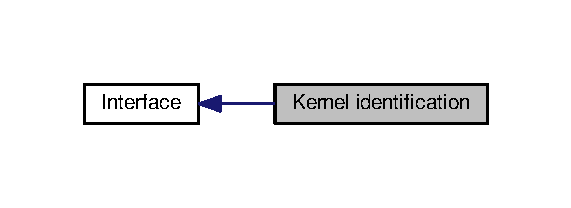
\includegraphics[width=274pt]{group__kern__id}
\end{center}
\end{figure}
\subsubsection*{Macros}
\begin{DoxyCompactItemize}
\item 
\#define \hyperlink{group__kern__id_ga06861cd0f6159ea9578193418c4eedf3}{E\-S\-\_\-\-K\-E\-R\-N\-\_\-\-V\-E\-R\-\_\-\-M\-A\-J\-O\-R}~1ul
\begin{DoxyCompactList}\small\item\em Identifies kernel major version number. \end{DoxyCompactList}\item 
\#define \hyperlink{group__kern__id_gaba74930b21c9c629a2589437f1e2584c}{E\-S\-\_\-\-K\-E\-R\-N\-\_\-\-V\-E\-R\-\_\-\-M\-I\-N\-O\-R}~0ul
\begin{DoxyCompactList}\small\item\em Identifies kernel minor version number. \end{DoxyCompactList}\item 
\#define \hyperlink{group__kern__id_gaa04466b958eeef9d02afadd6481abe5f}{E\-S\-\_\-\-K\-E\-R\-N\-\_\-\-V\-E\-R\-\_\-\-P\-A\-T\-C\-H}~0ul
\begin{DoxyCompactList}\small\item\em Identifies kernel patch level. \end{DoxyCompactList}\item 
\#define \hyperlink{group__kern__id_gacde22f7336a3c1c032dfc0ee3b94f506}{E\-S\-\_\-\-K\-E\-R\-N\-\_\-\-V\-E\-R}~(((\hyperlink{group__kern__id_ga06861cd0f6159ea9578193418c4eedf3}{E\-S\-\_\-\-K\-E\-R\-N\-\_\-\-V\-E\-R\-\_\-\-M\-A\-J\-O\-R}) $<$$<$ 24) $|$ (\hyperlink{group__kern__id_gaba74930b21c9c629a2589437f1e2584c}{E\-S\-\_\-\-K\-E\-R\-N\-\_\-\-V\-E\-R\-\_\-\-M\-I\-N\-O\-R} $<$$<$ 16) $|$ (\hyperlink{group__kern__id_gaa04466b958eeef9d02afadd6481abe5f}{E\-S\-\_\-\-K\-E\-R\-N\-\_\-\-V\-E\-R\-\_\-\-P\-A\-T\-C\-H}))
\begin{DoxyCompactList}\small\item\em Identifies the underlying kernel version number. \end{DoxyCompactList}\item 
\#define \hyperlink{group__kern__id_ga7a9484c6b09349e4eb82ba67c0989e25}{E\-S\-\_\-\-K\-E\-R\-N\-\_\-\-I\-D}~\char`\"{}e\-Solid -\/ R\-T Kernel\char`\"{}
\begin{DoxyCompactList}\small\item\em Kernel identification string. \end{DoxyCompactList}\end{DoxyCompactItemize}


\subsubsection{Detailed Description}
Kernel unique identification and current version number. 

\subsubsection{Macro Definition Documentation}
\hypertarget{group__kern__id_ga06861cd0f6159ea9578193418c4eedf3}{\index{Kernel identification@{Kernel identification}!E\-S\-\_\-\-K\-E\-R\-N\-\_\-\-V\-E\-R\-\_\-\-M\-A\-J\-O\-R@{E\-S\-\_\-\-K\-E\-R\-N\-\_\-\-V\-E\-R\-\_\-\-M\-A\-J\-O\-R}}
\index{E\-S\-\_\-\-K\-E\-R\-N\-\_\-\-V\-E\-R\-\_\-\-M\-A\-J\-O\-R@{E\-S\-\_\-\-K\-E\-R\-N\-\_\-\-V\-E\-R\-\_\-\-M\-A\-J\-O\-R}!Kernel identification@{Kernel identification}}
\paragraph[{E\-S\-\_\-\-K\-E\-R\-N\-\_\-\-V\-E\-R\-\_\-\-M\-A\-J\-O\-R}]{\setlength{\rightskip}{0pt plus 5cm}\#define E\-S\-\_\-\-K\-E\-R\-N\-\_\-\-V\-E\-R\-\_\-\-M\-A\-J\-O\-R~1ul}}\label{group__kern__id_ga06861cd0f6159ea9578193418c4eedf3}


Identifies kernel major version number. 

\hypertarget{group__kern__id_gaba74930b21c9c629a2589437f1e2584c}{\index{Kernel identification@{Kernel identification}!E\-S\-\_\-\-K\-E\-R\-N\-\_\-\-V\-E\-R\-\_\-\-M\-I\-N\-O\-R@{E\-S\-\_\-\-K\-E\-R\-N\-\_\-\-V\-E\-R\-\_\-\-M\-I\-N\-O\-R}}
\index{E\-S\-\_\-\-K\-E\-R\-N\-\_\-\-V\-E\-R\-\_\-\-M\-I\-N\-O\-R@{E\-S\-\_\-\-K\-E\-R\-N\-\_\-\-V\-E\-R\-\_\-\-M\-I\-N\-O\-R}!Kernel identification@{Kernel identification}}
\paragraph[{E\-S\-\_\-\-K\-E\-R\-N\-\_\-\-V\-E\-R\-\_\-\-M\-I\-N\-O\-R}]{\setlength{\rightskip}{0pt plus 5cm}\#define E\-S\-\_\-\-K\-E\-R\-N\-\_\-\-V\-E\-R\-\_\-\-M\-I\-N\-O\-R~0ul}}\label{group__kern__id_gaba74930b21c9c629a2589437f1e2584c}


Identifies kernel minor version number. 

\hypertarget{group__kern__id_gaa04466b958eeef9d02afadd6481abe5f}{\index{Kernel identification@{Kernel identification}!E\-S\-\_\-\-K\-E\-R\-N\-\_\-\-V\-E\-R\-\_\-\-P\-A\-T\-C\-H@{E\-S\-\_\-\-K\-E\-R\-N\-\_\-\-V\-E\-R\-\_\-\-P\-A\-T\-C\-H}}
\index{E\-S\-\_\-\-K\-E\-R\-N\-\_\-\-V\-E\-R\-\_\-\-P\-A\-T\-C\-H@{E\-S\-\_\-\-K\-E\-R\-N\-\_\-\-V\-E\-R\-\_\-\-P\-A\-T\-C\-H}!Kernel identification@{Kernel identification}}
\paragraph[{E\-S\-\_\-\-K\-E\-R\-N\-\_\-\-V\-E\-R\-\_\-\-P\-A\-T\-C\-H}]{\setlength{\rightskip}{0pt plus 5cm}\#define E\-S\-\_\-\-K\-E\-R\-N\-\_\-\-V\-E\-R\-\_\-\-P\-A\-T\-C\-H~0ul}}\label{group__kern__id_gaa04466b958eeef9d02afadd6481abe5f}


Identifies kernel patch level. 

\hypertarget{group__kern__id_gacde22f7336a3c1c032dfc0ee3b94f506}{\index{Kernel identification@{Kernel identification}!E\-S\-\_\-\-K\-E\-R\-N\-\_\-\-V\-E\-R@{E\-S\-\_\-\-K\-E\-R\-N\-\_\-\-V\-E\-R}}
\index{E\-S\-\_\-\-K\-E\-R\-N\-\_\-\-V\-E\-R@{E\-S\-\_\-\-K\-E\-R\-N\-\_\-\-V\-E\-R}!Kernel identification@{Kernel identification}}
\paragraph[{E\-S\-\_\-\-K\-E\-R\-N\-\_\-\-V\-E\-R}]{\setlength{\rightskip}{0pt plus 5cm}\#define E\-S\-\_\-\-K\-E\-R\-N\-\_\-\-V\-E\-R~((({\bf E\-S\-\_\-\-K\-E\-R\-N\-\_\-\-V\-E\-R\-\_\-\-M\-A\-J\-O\-R}) $<$$<$ 24) $|$ ({\bf E\-S\-\_\-\-K\-E\-R\-N\-\_\-\-V\-E\-R\-\_\-\-M\-I\-N\-O\-R} $<$$<$ 16) $|$ ({\bf E\-S\-\_\-\-K\-E\-R\-N\-\_\-\-V\-E\-R\-\_\-\-P\-A\-T\-C\-H}))}}\label{group__kern__id_gacde22f7336a3c1c032dfc0ee3b94f506}


Identifies the underlying kernel version number. 

\hypertarget{group__kern__id_ga7a9484c6b09349e4eb82ba67c0989e25}{\index{Kernel identification@{Kernel identification}!E\-S\-\_\-\-K\-E\-R\-N\-\_\-\-I\-D@{E\-S\-\_\-\-K\-E\-R\-N\-\_\-\-I\-D}}
\index{E\-S\-\_\-\-K\-E\-R\-N\-\_\-\-I\-D@{E\-S\-\_\-\-K\-E\-R\-N\-\_\-\-I\-D}!Kernel identification@{Kernel identification}}
\paragraph[{E\-S\-\_\-\-K\-E\-R\-N\-\_\-\-I\-D}]{\setlength{\rightskip}{0pt plus 5cm}\#define E\-S\-\_\-\-K\-E\-R\-N\-\_\-\-I\-D~\char`\"{}e\-Solid -\/ R\-T Kernel\char`\"{}}}\label{group__kern__id_ga7a9484c6b09349e4eb82ba67c0989e25}


Kernel identification string. 


\hypertarget{group__kern__thd}{\subsection{Thread}
\label{group__kern__thd}\index{Thread@{Thread}}
}


Thread management services.  


Collaboration diagram for Thread\-:\nopagebreak
\begin{figure}[H]
\begin{center}
\leavevmode
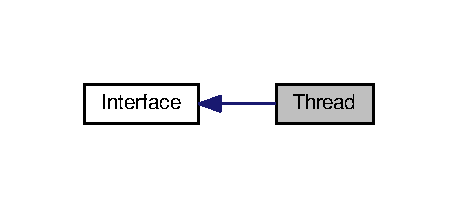
\includegraphics[width=220pt]{group__kern__thd}
\end{center}
\end{figure}
\subsubsection*{Data Structures}
\begin{DoxyCompactItemize}
\item 
struct \hyperlink{structesThd}{es\-Thd}
\begin{DoxyCompactList}\small\item\em Thread structure. \end{DoxyCompactList}\end{DoxyCompactItemize}
\subsubsection*{Macros}
\begin{DoxyCompactItemize}
\item 
\#define \hyperlink{group__kern__thd_gaa707debebe3f98439911212b0cc8b3d1}{E\-S\-\_\-\-S\-T\-C\-K\-\_\-\-S\-I\-Z\-E}(elem)~\hyperlink{group__template__cpu__intf_gacb3a46e89d327fbaf5c122fe23877b24}{P\-O\-R\-T\-\_\-\-S\-T\-C\-K\-\_\-\-S\-I\-Z\-E}(elem)
\begin{DoxyCompactList}\small\item\em Converts the required stack elements into the stack array index. \end{DoxyCompactList}\item 
\#define \hyperlink{group__kern__thd_gaa9562c0ae61ad207e40486f952c5c7b3}{E\-S\-\_\-\-D\-E\-F\-\_\-\-T\-H\-D\-\_\-\-P\-R\-I\-O\-\_\-\-M\-A\-X}~(\hyperlink{group__template__kern__cfg_ga56bd89fe76f7fe22f3d8805bc3c68892}{C\-F\-G\-\_\-\-S\-C\-H\-E\-D\-\_\-\-P\-R\-I\-O\-\_\-\-L\-V\-L} -\/ 2u)
\begin{DoxyCompactList}\small\item\em Maximum level of priority possible for application thread. \end{DoxyCompactList}\item 
\#define \hyperlink{group__kern__thd_ga4dc54b2d44aa0656de70c7357733f4e4}{E\-S\-\_\-\-D\-E\-F\-\_\-\-T\-H\-D\-\_\-\-P\-R\-I\-O\-\_\-\-M\-I\-N}~(1u)
\begin{DoxyCompactList}\small\item\em Minimum level of priority possible for application thread. \end{DoxyCompactList}\end{DoxyCompactItemize}
\subsubsection*{Typedefs}
\begin{DoxyCompactItemize}
\item 
typedef struct \hyperlink{structesThd}{es\-Thd} \hyperlink{group__kern__thd_ga62e3a3ca0a4597a19c43cb8868810d82}{es\-Thd\-\_\-\-T}
\begin{DoxyCompactList}\small\item\em Thread type. \end{DoxyCompactList}\item 
typedef \hyperlink{group__template__cpu__intf_ga13cc91970e3e05fe4210440c068d3f4a}{port\-Stck\-\_\-\-T} \hyperlink{group__kern__thd_ga24160ddd0cb0327108cc652bfe6a49e5}{es\-Stck\-\_\-\-T}
\begin{DoxyCompactList}\small\item\em Stack type. \end{DoxyCompactList}\end{DoxyCompactItemize}
\subsubsection*{Functions}
\begin{DoxyCompactItemize}
\item 
void \hyperlink{group__kern__thd_gac91734f3ee867b519f59bf81cc7fde88}{es\-Thd\-Init} (\hyperlink{group__kern__thd_ga62e3a3ca0a4597a19c43cb8868810d82}{es\-Thd\-\_\-\-T} $\ast$thd, void($\ast$fn)(void $\ast$), void $\ast$arg, \hyperlink{group__template__cpu__intf_ga13cc91970e3e05fe4210440c068d3f4a}{port\-Stck\-\_\-\-T} $\ast$stck, size\-\_\-t stck\-Size, uint8\-\_\-t prio)
\begin{DoxyCompactList}\small\item\em Initialize the specified thread. \end{DoxyCompactList}\item 
void \hyperlink{group__kern__thd_gac9d1eac76f26096614e8196bcfd8b905}{es\-Thd\-Term} (\hyperlink{group__kern__thd_ga62e3a3ca0a4597a19c43cb8868810d82}{es\-Thd\-\_\-\-T} $\ast$thd)
\begin{DoxyCompactList}\small\item\em Terminate the specified thread. \end{DoxyCompactList}\item 
static \hyperlink{group__template__compiler_ga87952d6e574c7f437503926e833ba345}{P\-O\-R\-T\-\_\-\-C\-\_\-\-I\-N\-L\-I\-N\-E} \hyperlink{group__kern__thd_ga62e3a3ca0a4597a19c43cb8868810d82}{es\-Thd\-\_\-\-T} $\ast$ \hyperlink{group__kern__thd_gae2a2c5fe0128d446a64512b0714bfb6d}{es\-Thd\-Get\-Id} (void)
\begin{DoxyCompactList}\small\item\em Get the current thread I\-D. \end{DoxyCompactList}\item 
static \hyperlink{group__template__compiler_ga87952d6e574c7f437503926e833ba345}{P\-O\-R\-T\-\_\-\-C\-\_\-\-I\-N\-L\-I\-N\-E} uint8\-\_\-t \hyperlink{group__kern__thd_ga6d2d033dc7e1226eccf4a51c666678ad}{es\-Thd\-Get\-Prio} (\hyperlink{group__kern__thd_ga62e3a3ca0a4597a19c43cb8868810d82}{es\-Thd\-\_\-\-T} $\ast$thd)
\begin{DoxyCompactList}\small\item\em Get the priority of a thread. \end{DoxyCompactList}\item 
void \hyperlink{group__kern__thd_ga8eaa731d0026a8a1667d4422d5031df6}{es\-Thd\-Set\-Prio\-I} (\hyperlink{group__kern__thd_ga62e3a3ca0a4597a19c43cb8868810d82}{es\-Thd\-\_\-\-T} $\ast$thd, uint8\-\_\-t prio)
\begin{DoxyCompactList}\small\item\em Set the priority of a thread. \end{DoxyCompactList}\end{DoxyCompactItemize}


\subsubsection{Detailed Description}
Thread management services. For more details see \hyperlink{threads}{Thread Management}. 

\subsubsection{Macro Definition Documentation}
\hypertarget{group__kern__thd_gaa707debebe3f98439911212b0cc8b3d1}{\index{Thread@{Thread}!E\-S\-\_\-\-S\-T\-C\-K\-\_\-\-S\-I\-Z\-E@{E\-S\-\_\-\-S\-T\-C\-K\-\_\-\-S\-I\-Z\-E}}
\index{E\-S\-\_\-\-S\-T\-C\-K\-\_\-\-S\-I\-Z\-E@{E\-S\-\_\-\-S\-T\-C\-K\-\_\-\-S\-I\-Z\-E}!Thread@{Thread}}
\paragraph[{E\-S\-\_\-\-S\-T\-C\-K\-\_\-\-S\-I\-Z\-E}]{\setlength{\rightskip}{0pt plus 5cm}\#define E\-S\-\_\-\-S\-T\-C\-K\-\_\-\-S\-I\-Z\-E(
\begin{DoxyParamCaption}
\item[{}]{elem}
\end{DoxyParamCaption}
)~{\bf P\-O\-R\-T\-\_\-\-S\-T\-C\-K\-\_\-\-S\-I\-Z\-E}(elem)}}\label{group__kern__thd_gaa707debebe3f98439911212b0cc8b3d1}


Converts the required stack elements into the stack array index. 


\begin{DoxyParams}{Parameters}
{\em elem} & Number of stack elements\-: the stack size is expressed in number of elements regardless of the size of port general purpose registers. \\
\hline
\end{DoxyParams}
\begin{DoxyReturn}{Returns}
Number of stack elements needed for stack usage. 
\end{DoxyReturn}
\hypertarget{group__kern__thd_gaa9562c0ae61ad207e40486f952c5c7b3}{\index{Thread@{Thread}!E\-S\-\_\-\-D\-E\-F\-\_\-\-T\-H\-D\-\_\-\-P\-R\-I\-O\-\_\-\-M\-A\-X@{E\-S\-\_\-\-D\-E\-F\-\_\-\-T\-H\-D\-\_\-\-P\-R\-I\-O\-\_\-\-M\-A\-X}}
\index{E\-S\-\_\-\-D\-E\-F\-\_\-\-T\-H\-D\-\_\-\-P\-R\-I\-O\-\_\-\-M\-A\-X@{E\-S\-\_\-\-D\-E\-F\-\_\-\-T\-H\-D\-\_\-\-P\-R\-I\-O\-\_\-\-M\-A\-X}!Thread@{Thread}}
\paragraph[{E\-S\-\_\-\-D\-E\-F\-\_\-\-T\-H\-D\-\_\-\-P\-R\-I\-O\-\_\-\-M\-A\-X}]{\setlength{\rightskip}{0pt plus 5cm}\#define E\-S\-\_\-\-D\-E\-F\-\_\-\-T\-H\-D\-\_\-\-P\-R\-I\-O\-\_\-\-M\-A\-X~({\bf C\-F\-G\-\_\-\-S\-C\-H\-E\-D\-\_\-\-P\-R\-I\-O\-\_\-\-L\-V\-L} -\/ 2u)}}\label{group__kern__thd_gaa9562c0ae61ad207e40486f952c5c7b3}


Maximum level of priority possible for application thread. 

\hypertarget{group__kern__thd_ga4dc54b2d44aa0656de70c7357733f4e4}{\index{Thread@{Thread}!E\-S\-\_\-\-D\-E\-F\-\_\-\-T\-H\-D\-\_\-\-P\-R\-I\-O\-\_\-\-M\-I\-N@{E\-S\-\_\-\-D\-E\-F\-\_\-\-T\-H\-D\-\_\-\-P\-R\-I\-O\-\_\-\-M\-I\-N}}
\index{E\-S\-\_\-\-D\-E\-F\-\_\-\-T\-H\-D\-\_\-\-P\-R\-I\-O\-\_\-\-M\-I\-N@{E\-S\-\_\-\-D\-E\-F\-\_\-\-T\-H\-D\-\_\-\-P\-R\-I\-O\-\_\-\-M\-I\-N}!Thread@{Thread}}
\paragraph[{E\-S\-\_\-\-D\-E\-F\-\_\-\-T\-H\-D\-\_\-\-P\-R\-I\-O\-\_\-\-M\-I\-N}]{\setlength{\rightskip}{0pt plus 5cm}\#define E\-S\-\_\-\-D\-E\-F\-\_\-\-T\-H\-D\-\_\-\-P\-R\-I\-O\-\_\-\-M\-I\-N~(1u)}}\label{group__kern__thd_ga4dc54b2d44aa0656de70c7357733f4e4}


Minimum level of priority possible for application thread. 



\subsubsection{Typedef Documentation}
\hypertarget{group__kern__thd_ga62e3a3ca0a4597a19c43cb8868810d82}{\index{Thread@{Thread}!es\-Thd\-\_\-\-T@{es\-Thd\-\_\-\-T}}
\index{es\-Thd\-\_\-\-T@{es\-Thd\-\_\-\-T}!Thread@{Thread}}
\paragraph[{es\-Thd\-\_\-\-T}]{\setlength{\rightskip}{0pt plus 5cm}typedef struct {\bf es\-Thd} {\bf es\-Thd\-\_\-\-T}}}\label{group__kern__thd_ga62e3a3ca0a4597a19c43cb8868810d82}


Thread type. 

\hypertarget{group__kern__thd_ga24160ddd0cb0327108cc652bfe6a49e5}{\index{Thread@{Thread}!es\-Stck\-\_\-\-T@{es\-Stck\-\_\-\-T}}
\index{es\-Stck\-\_\-\-T@{es\-Stck\-\_\-\-T}!Thread@{Thread}}
\paragraph[{es\-Stck\-\_\-\-T}]{\setlength{\rightskip}{0pt plus 5cm}typedef {\bf port\-Stck\-\_\-\-T} {\bf es\-Stck\-\_\-\-T}}}\label{group__kern__thd_ga24160ddd0cb0327108cc652bfe6a49e5}


Stack type. 



\subsubsection{Function Documentation}
\hypertarget{group__kern__thd_gac91734f3ee867b519f59bf81cc7fde88}{\index{Thread@{Thread}!es\-Thd\-Init@{es\-Thd\-Init}}
\index{es\-Thd\-Init@{es\-Thd\-Init}!Thread@{Thread}}
\paragraph[{es\-Thd\-Init}]{\setlength{\rightskip}{0pt plus 5cm}void es\-Thd\-Init (
\begin{DoxyParamCaption}
\item[{{\bf es\-Thd\-\_\-\-T} $\ast$}]{thd, }
\item[{void($\ast$)(void $\ast$)}]{fn, }
\item[{void $\ast$}]{arg, }
\item[{{\bf port\-Stck\-\_\-\-T} $\ast$}]{stck, }
\item[{size\-\_\-t}]{stck\-Size, }
\item[{uint8\-\_\-t}]{prio}
\end{DoxyParamCaption}
)}}\label{group__kern__thd_gac91734f3ee867b519f59bf81cc7fde88}


Initialize the specified thread. 


\begin{DoxyParams}{Parameters}
{\em thd} & Thread\-: is a pointer to the thread structure, \hyperlink{structesThd}{es\-Thd}. The structure will be used as information container for the thread. It is assumed that storage for the {\ttfamily \hyperlink{structesThd}{es\-Thd}} structure is allocated by the user code. \\
\hline
{\em fn} & Function\-: is a pointer to thread function. Thread function must have the following signature\-: {\ttfamily void thread (void $\ast$ arg)}. \\
\hline
{\em arg} & Argument\-: is a void pointer to an optional data area. It's usage is application defined and it is intended to pass arguments to thread when it is started for the first time. \\
\hline
{\em stck} & Stack\-: is a pointer to a allocated memory for thread stack. The pointer always points to the first element in the array, regardless of what type of stack the C\-P\-U is using. The thread's stack is used to store local variables, function parameters, return addresses. Each thread has its own stack and different sized stack. The stack type must be an array of \hyperlink{structportStck}{port\-Stck}. \\
\hline
{\em stck\-Size} & Stack Size\-: specifies the size of allocated stack memory. Size is expressed in bytes. Please see port documentation about minimal stack size. Usage of C unary operator {\ttfamily sizeof} is the recommended way of specifying stack size. Another way of specifying required stack size is through the usage of \hyperlink{group__kern__thd_gaa707debebe3f98439911212b0cc8b3d1}{E\-S\-\_\-\-S\-T\-C\-K\-\_\-\-S\-I\-Z\-E} macro. \\
\hline
{\em prio} & Priority\-: is the priority of the thread. The higher the number, the higher the priority (the importance) of the thread. Several threads can have the same priority. Note that lowest (0) and highest (C\-F\-G\-\_\-\-S\-C\-H\-E\-D\-\_\-\-P\-R\-I\-O\-\_\-\-L\-V\-L -\/ 1) levels are reserved for kernel threads only. \\
\hline
\end{DoxyParams}
\begin{DoxyPrecond}{Precondition}
1) {\ttfamily The kernel state E\-S\-\_\-\-K\-E\-R\-N\-\_\-\-I\-N\-A\-C\-T\-I\-V\-E}, see \hyperlink{states}{Kernel states}. 

2) {\ttfamily thd != N\-U\-L\-L} 

3) {\ttfamily thd-\/$>$signature != D\-E\-F\-\_\-\-T\-H\-D\-\_\-\-C\-O\-N\-T\-R\-A\-C\-T\-\_\-\-S\-I\-G\-N\-A\-T\-U\-R\-E}, the thread structure can't be initialized more than once. 

4) {\ttfamily fn != N\-U\-L\-L} 

5) {\ttfamily stck\-Size $>$= P\-O\-R\-T\-\_\-\-D\-E\-F\-\_\-\-S\-T\-C\-K\-\_\-\-M\-I\-N\-S\-I\-Z\-E}, see \hyperlink{group__template__cpu__intf_ga5a629fee11006b5b0b97f7cb7176efd4}{P\-O\-R\-T\-\_\-\-D\-E\-F\-\_\-\-S\-T\-C\-K\-\_\-\-M\-I\-N\-S\-I\-Z\-E}. 

6) {\ttfamily 0 $<$ prio $<$ C\-F\-G\-\_\-\-S\-C\-H\-E\-D\-\_\-\-P\-R\-I\-O\-\_\-\-L\-V\-L -\/ 1}, see \hyperlink{group__template__kern__cfg_ga56bd89fe76f7fe22f3d8805bc3c68892}{C\-F\-G\-\_\-\-S\-C\-H\-E\-D\-\_\-\-P\-R\-I\-O\-\_\-\-L\-V\-L}. 
\end{DoxyPrecond}
\begin{DoxyPostcond}{Postcondition}
1) {\ttfamily thd-\/$>$signature == D\-E\-F\-\_\-\-T\-H\-D\-\_\-\-C\-O\-N\-T\-R\-A\-C\-T\-\_\-\-S\-I\-G\-N\-A\-T\-U\-R\-E}, each \hyperlink{structesThd}{es\-Thd} structure will have valid signature after initialization.
\end{DoxyPostcond}
Threads must be created in order for kernel to recognize them as threads. Initialize a thread by calling \hyperlink{group__kern__thd_gac91734f3ee867b519f59bf81cc7fde88}{es\-Thd\-Init()} and provide arguments specifying to kernel how the thread will be managed. Threads are always created in the {\ttfamily ready-\/to-\/run} state. Threads can be created either prior to the start of multi-\/threading (before calling \hyperlink{group__kern__general_ga0e7a0a6b9c02df58de0f98de0229a09d}{es\-Kern\-Start()}), or by a running thread. \begin{DoxyParagraph}{This service can be called from\-:}

\begin{DoxyItemize}
\item Application initialization code
\item Application thread code 
\end{DoxyItemize}
\end{DoxyParagraph}
\begin{DoxyParagraph}{Rescheduling\-:}

\begin{DoxyItemize}
\item possible 
\end{DoxyItemize}
\end{DoxyParagraph}
\begin{DoxyParagraph}{Object class\-:}
Regular {\bfseries A\-P\-I} object, this object is part of the application programming interface. 
\end{DoxyParagraph}
\hypertarget{group__kern__thd_gac9d1eac76f26096614e8196bcfd8b905}{\index{Thread@{Thread}!es\-Thd\-Term@{es\-Thd\-Term}}
\index{es\-Thd\-Term@{es\-Thd\-Term}!Thread@{Thread}}
\paragraph[{es\-Thd\-Term}]{\setlength{\rightskip}{0pt plus 5cm}void es\-Thd\-Term (
\begin{DoxyParamCaption}
\item[{{\bf es\-Thd\-\_\-\-T} $\ast$}]{thd}
\end{DoxyParamCaption}
)}}\label{group__kern__thd_gac9d1eac76f26096614e8196bcfd8b905}


Terminate the specified thread. 


\begin{DoxyParams}{Parameters}
{\em thd} & Thread\-: is a pointer to the thread structure, \hyperlink{structesThd}{es\-Thd}. \\
\hline
\end{DoxyParams}
\begin{DoxyPrecond}{Precondition}
1) {\ttfamily The kernel state E\-S\-\_\-\-K\-E\-R\-N\-\_\-\-I\-N\-A\-C\-T\-I\-V\-E}, see \hyperlink{states}{Kernel states}. 

2) {\ttfamily thd != N\-U\-L\-L} 

3) {\ttfamily thd-\/$>$signature == D\-E\-F\-\_\-\-T\-H\-D\-\_\-\-C\-O\-N\-T\-R\-A\-C\-T\-\_\-\-S\-I\-G\-N\-A\-T\-U\-R\-E}, the pointer must point to a valid \hyperlink{structesThd}{es\-Thd} structure. 

4) {\ttfamily (thd-\/$>$thd\-L\-\_\-.\-q == N\-U\-L\-L) O\-R (thd-\/$>$thd\-L\-\_\-.\-q == g\-Rdy\-Queue)}, thread must be either in Ready Threads Queue or not be in any queue (e.\-g. not waiting for a synchronization mechanism). 
\end{DoxyPrecond}
\begin{DoxyPostcond}{Postcondition}
1) {\ttfamily thd-\/$>$signature == $\sim$\-D\-E\-F\-\_\-\-T\-H\-D\-\_\-\-C\-O\-N\-T\-R\-A\-C\-T\-\_\-\-S\-I\-G\-N\-A\-T\-U\-R\-E}, each \hyperlink{structesThd}{es\-Thd} structure will have invalid signature after termination. 
\end{DoxyPostcond}
\begin{DoxyParagraph}{This service can be called from\-:}

\begin{DoxyItemize}
\item Application initialization code
\item Application thread code 
\end{DoxyItemize}
\end{DoxyParagraph}
\begin{DoxyParagraph}{Rescheduling\-:}

\begin{DoxyItemize}
\item possible 
\end{DoxyItemize}
\end{DoxyParagraph}
\begin{DoxyParagraph}{Object class\-:}
Regular {\bfseries A\-P\-I} object, this object is part of the application programming interface. 
\end{DoxyParagraph}
\hypertarget{group__kern__thd_gae2a2c5fe0128d446a64512b0714bfb6d}{\index{Thread@{Thread}!es\-Thd\-Get\-Id@{es\-Thd\-Get\-Id}}
\index{es\-Thd\-Get\-Id@{es\-Thd\-Get\-Id}!Thread@{Thread}}
\paragraph[{es\-Thd\-Get\-Id}]{\setlength{\rightskip}{0pt plus 5cm}static {\bf P\-O\-R\-T\-\_\-\-C\-\_\-\-I\-N\-L\-I\-N\-E} {\bf es\-Thd\-\_\-\-T}$\ast$ es\-Thd\-Get\-Id (
\begin{DoxyParamCaption}
\item[{void}]{}
\end{DoxyParamCaption}
)\hspace{0.3cm}{\ttfamily [static]}}}\label{group__kern__thd_gae2a2c5fe0128d446a64512b0714bfb6d}


Get the current thread I\-D. 

\begin{DoxyReturn}{Returns}
Pointer to current thread I\-D structure \hyperlink{structesThd}{es\-Thd}. 
\end{DoxyReturn}
\begin{DoxyNote}{Note}
This is {\ttfamily inline} function. 
\end{DoxyNote}
\begin{DoxyParagraph}{This service can be called from\-:}

\begin{DoxyItemize}
\item Application initialization code
\item Application thread code
\item Interrupt service routine 
\end{DoxyItemize}
\end{DoxyParagraph}
\begin{DoxyParagraph}{Rescheduling\-:}

\begin{DoxyItemize}
\item never 
\end{DoxyItemize}
\end{DoxyParagraph}
\begin{DoxyParagraph}{Object class\-:}
Regular {\bfseries A\-P\-I} object, this object is part of the application programming interface. 
\end{DoxyParagraph}
\hypertarget{group__kern__thd_ga6d2d033dc7e1226eccf4a51c666678ad}{\index{Thread@{Thread}!es\-Thd\-Get\-Prio@{es\-Thd\-Get\-Prio}}
\index{es\-Thd\-Get\-Prio@{es\-Thd\-Get\-Prio}!Thread@{Thread}}
\paragraph[{es\-Thd\-Get\-Prio}]{\setlength{\rightskip}{0pt plus 5cm}static {\bf P\-O\-R\-T\-\_\-\-C\-\_\-\-I\-N\-L\-I\-N\-E} uint8\-\_\-t es\-Thd\-Get\-Prio (
\begin{DoxyParamCaption}
\item[{{\bf es\-Thd\-\_\-\-T} $\ast$}]{thd}
\end{DoxyParamCaption}
)\hspace{0.3cm}{\ttfamily [static]}}}\label{group__kern__thd_ga6d2d033dc7e1226eccf4a51c666678ad}


Get the priority of a thread. 


\begin{DoxyParams}{Parameters}
{\em thd} & Thread\-: is pointer to the thread structure, \hyperlink{structesThd}{es\-Thd}. \\
\hline
\end{DoxyParams}
\begin{DoxyReturn}{Returns}
The priority of the thread pointed by {\ttfamily thd}. 
\end{DoxyReturn}
\begin{DoxyNote}{Note}
This is {\ttfamily inline} function. 
\end{DoxyNote}
\begin{DoxyParagraph}{This service can be called from\-:}

\begin{DoxyItemize}
\item Application initialization code
\item Application thread code
\item Interrupt service routine 
\end{DoxyItemize}
\end{DoxyParagraph}
\begin{DoxyParagraph}{Rescheduling\-:}

\begin{DoxyItemize}
\item never 
\end{DoxyItemize}
\end{DoxyParagraph}
\begin{DoxyParagraph}{Object class\-:}
Regular {\bfseries A\-P\-I} object, this object is part of the application programming interface. 
\end{DoxyParagraph}
\hypertarget{group__kern__thd_ga8eaa731d0026a8a1667d4422d5031df6}{\index{Thread@{Thread}!es\-Thd\-Set\-Prio\-I@{es\-Thd\-Set\-Prio\-I}}
\index{es\-Thd\-Set\-Prio\-I@{es\-Thd\-Set\-Prio\-I}!Thread@{Thread}}
\paragraph[{es\-Thd\-Set\-Prio\-I}]{\setlength{\rightskip}{0pt plus 5cm}void es\-Thd\-Set\-Prio\-I (
\begin{DoxyParamCaption}
\item[{{\bf es\-Thd\-\_\-\-T} $\ast$}]{thd, }
\item[{uint8\-\_\-t}]{prio}
\end{DoxyParamCaption}
)}}\label{group__kern__thd_ga8eaa731d0026a8a1667d4422d5031df6}


Set the priority of a thread. 


\begin{DoxyParams}{Parameters}
{\em thd} & Thread\-: is pointer to the thread structure, \hyperlink{structesThd}{es\-Thd}. \\
\hline
{\em prio} & Priority\-: is new priority of the thread pointed by {\ttfamily thd}. \\
\hline
\end{DoxyParams}
\begin{DoxyPrecond}{Precondition}
1) {\ttfamily The kernel state $<$ E\-S\-\_\-\-K\-E\-R\-N\-\_\-\-I\-N\-A\-C\-T\-I\-V\-E}, see \hyperlink{states}{Kernel states}. 

2) {\ttfamily thd != N\-U\-L\-L} 

3) {\ttfamily thd-\/$>$signature == D\-E\-F\-\_\-\-T\-H\-D\-\_\-\-C\-O\-N\-T\-R\-A\-C\-T\-\_\-\-S\-I\-G\-N\-A\-T\-U\-R\-E}, the pointer must point to a valid \hyperlink{structesThd}{es\-Thd} structure. 

4) {\ttfamily 0 $<$ prio $<$ C\-F\-G\-\_\-\-S\-C\-H\-E\-D\-\_\-\-P\-R\-I\-O\-\_\-\-L\-V\-L -\/ 1}, see \hyperlink{group__template__kern__cfg_ga56bd89fe76f7fe22f3d8805bc3c68892}{C\-F\-G\-\_\-\-S\-C\-H\-E\-D\-\_\-\-P\-R\-I\-O\-\_\-\-L\-V\-L}. 
\end{DoxyPrecond}
\begin{DoxyParagraph}{This service can be called from\-:}

\begin{DoxyItemize}
\item Application initialization code
\item Application thread code
\item Interrupt service routine 
\end{DoxyItemize}
\end{DoxyParagraph}
\begin{DoxyParagraph}{Rescheduling\-:}

\begin{DoxyItemize}
\item possible 
\end{DoxyItemize}
\end{DoxyParagraph}
\begin{DoxyParagraph}{Function class\-:}
{\bfseries I class}, Interrupt-\/lock A\-P\-I function, this function can be called only from interrupts locked code sections. 
\end{DoxyParagraph}

\hypertarget{group__kern__thdq}{\subsection{Thread Queue}
\label{group__kern__thdq}\index{Thread Queue@{Thread Queue}}
}


Thread Queue management services.  


Collaboration diagram for Thread Queue\-:\nopagebreak
\begin{figure}[H]
\begin{center}
\leavevmode
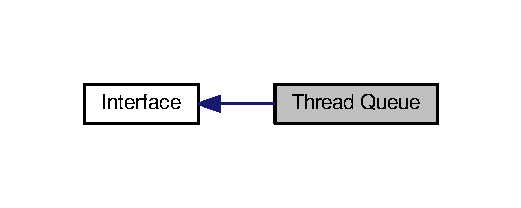
\includegraphics[width=250pt]{group__kern__thdq}
\end{center}
\end{figure}
\subsubsection*{Data Structures}
\begin{DoxyCompactItemize}
\item 
struct \hyperlink{structesThdQ}{es\-Thd\-Q}
\begin{DoxyCompactList}\small\item\em Thread Queue structure. \end{DoxyCompactList}\end{DoxyCompactItemize}
\subsubsection*{Typedefs}
\begin{DoxyCompactItemize}
\item 
typedef struct \hyperlink{structesThdQ}{es\-Thd\-Q} \hyperlink{group__kern__thdq_ga7a1a060699e83a01512ebb5540019556}{es\-Thd\-Q\-\_\-\-T}
\begin{DoxyCompactList}\small\item\em Thread queue type. \end{DoxyCompactList}\end{DoxyCompactItemize}
\subsubsection*{Functions}
\begin{DoxyCompactItemize}
\item 
void \hyperlink{group__kern__thdq_gaddd5fe0557c91559b9452beb0fc236fd}{es\-Thd\-Q\-Init} (\hyperlink{group__kern__thdq_ga7a1a060699e83a01512ebb5540019556}{es\-Thd\-Q\-\_\-\-T} $\ast$thd\-Q)
\begin{DoxyCompactList}\small\item\em Initialize Thread Queue. \end{DoxyCompactList}\item 
void \hyperlink{group__kern__thdq_gaa5f19b32a7f0c42616b5270dcbd73a3e}{es\-Thd\-Q\-Term} (\hyperlink{group__kern__thdq_ga7a1a060699e83a01512ebb5540019556}{es\-Thd\-Q\-\_\-\-T} $\ast$thd\-Q)
\begin{DoxyCompactList}\small\item\em Terminate Thread Queue. \end{DoxyCompactList}\item 
void \hyperlink{group__kern__thdq_ga9da1e71c137d8adb8c9bdead7052b5fa}{es\-Thd\-Q\-Add\-I} (\hyperlink{group__kern__thdq_ga7a1a060699e83a01512ebb5540019556}{es\-Thd\-Q\-\_\-\-T} $\ast$thd\-Q, \hyperlink{group__kern__thd_ga62e3a3ca0a4597a19c43cb8868810d82}{es\-Thd\-\_\-\-T} $\ast$thd)
\begin{DoxyCompactList}\small\item\em Add a thread to the Thread Queue. \end{DoxyCompactList}\item 
void \hyperlink{group__kern__thdq_gaa18afa95e34035da03c5cb7ea3a96320}{es\-Thd\-Q\-Rm\-I} (\hyperlink{group__kern__thdq_ga7a1a060699e83a01512ebb5540019556}{es\-Thd\-Q\-\_\-\-T} $\ast$thd\-Q, \hyperlink{group__kern__thd_ga62e3a3ca0a4597a19c43cb8868810d82}{es\-Thd\-\_\-\-T} $\ast$thd)
\begin{DoxyCompactList}\small\item\em Removes the thread from the Thread Queue. \end{DoxyCompactList}\item 
\hyperlink{group__kern__thd_ga62e3a3ca0a4597a19c43cb8868810d82}{es\-Thd\-\_\-\-T} $\ast$ \hyperlink{group__kern__thdq_ga1670c123f31c346b24ec9d2b7ae35f88}{es\-Thd\-Q\-Fetch\-I} (const \hyperlink{group__kern__thdq_ga7a1a060699e83a01512ebb5540019556}{es\-Thd\-Q\-\_\-\-T} $\ast$thd\-Q)
\begin{DoxyCompactList}\small\item\em Fetch the first high priority thread from the Thread Queue. \end{DoxyCompactList}\item 
\hyperlink{group__kern__thd_ga62e3a3ca0a4597a19c43cb8868810d82}{es\-Thd\-\_\-\-T} $\ast$ \hyperlink{group__kern__thdq_gae365b14292f1496a90d876baec84fb4e}{es\-Thd\-Q\-Fetch\-Rotate\-I} (\hyperlink{group__kern__thdq_ga7a1a060699e83a01512ebb5540019556}{es\-Thd\-Q\-\_\-\-T} $\ast$thd\-Q, uint\-\_\-fast8\-\_\-t prio)
\begin{DoxyCompactList}\small\item\em Fetch the next thread and rotate thread linked list. \end{DoxyCompactList}\item 
\hyperlink{group__template__compiler_ga74fbee312f9185efb602f89d21b53404}{bool\-\_\-\-T} \hyperlink{group__kern__thdq_gacf2687b82ce64e2154d97fd3b69a4ab5}{es\-Thd\-Q\-Is\-Empty} (const \hyperlink{group__kern__thdq_ga7a1a060699e83a01512ebb5540019556}{es\-Thd\-Q\-\_\-\-T} $\ast$thd\-Q)
\begin{DoxyCompactList}\small\item\em Is thread queue empty. \end{DoxyCompactList}\end{DoxyCompactItemize}


\subsubsection{Detailed Description}
Thread Queue management services. 

\subsubsection{Typedef Documentation}
\hypertarget{group__kern__thdq_ga7a1a060699e83a01512ebb5540019556}{\index{Thread Queue@{Thread Queue}!es\-Thd\-Q\-\_\-\-T@{es\-Thd\-Q\-\_\-\-T}}
\index{es\-Thd\-Q\-\_\-\-T@{es\-Thd\-Q\-\_\-\-T}!Thread Queue@{Thread Queue}}
\paragraph[{es\-Thd\-Q\-\_\-\-T}]{\setlength{\rightskip}{0pt plus 5cm}typedef struct {\bf es\-Thd\-Q} {\bf es\-Thd\-Q\-\_\-\-T}}}\label{group__kern__thdq_ga7a1a060699e83a01512ebb5540019556}


Thread queue type. 



\subsubsection{Function Documentation}
\hypertarget{group__kern__thdq_gaddd5fe0557c91559b9452beb0fc236fd}{\index{Thread Queue@{Thread Queue}!es\-Thd\-Q\-Init@{es\-Thd\-Q\-Init}}
\index{es\-Thd\-Q\-Init@{es\-Thd\-Q\-Init}!Thread Queue@{Thread Queue}}
\paragraph[{es\-Thd\-Q\-Init}]{\setlength{\rightskip}{0pt plus 5cm}void es\-Thd\-Q\-Init (
\begin{DoxyParamCaption}
\item[{{\bf es\-Thd\-Q\-\_\-\-T} $\ast$}]{thd\-Q}
\end{DoxyParamCaption}
)}}\label{group__kern__thdq_gaddd5fe0557c91559b9452beb0fc236fd}


Initialize Thread Queue. 


\begin{DoxyParams}{Parameters}
{\em thd\-Q} & Thread Queue\-: is a pointer to thread queue structure, \hyperlink{structesThdQ}{es\-Thd\-Q}. \\
\hline
\end{DoxyParams}
\begin{DoxyPrecond}{Precondition}
1) {\ttfamily thd\-Q != N\-U\-L\-L} 

2) {\ttfamily thd\-Q-\/$>$signature != D\-E\-F\-\_\-\-T\-H\-D\-Q\-\_\-\-C\-O\-N\-T\-R\-A\-C\-T\-\_\-\-S\-I\-G\-N\-A\-T\-U\-R\-E}, the thread queue structure can't be initialized more than once. 
\end{DoxyPrecond}
\begin{DoxyPostcond}{Postcondition}
1) {\ttfamily thd\-Q-\/$>$signature == D\-E\-F\-\_\-\-T\-H\-D\-Q\-\_\-\-C\-O\-N\-T\-R\-A\-C\-T\-\_\-\-S\-I\-G\-N\-A\-T\-U\-R\-E}, each \hyperlink{structesThdQ}{es\-Thd\-Q} structure will have valid signature after initialization. 
\end{DoxyPostcond}
\begin{DoxyParagraph}{This service can be called from\-:}

\begin{DoxyItemize}
\item Application initialization code
\item Application thread code
\item Interrupt service routine 
\end{DoxyItemize}
\end{DoxyParagraph}
\begin{DoxyParagraph}{Rescheduling\-:}

\begin{DoxyItemize}
\item never 
\end{DoxyItemize}
\end{DoxyParagraph}
\begin{DoxyParagraph}{Object class\-:}
Regular {\bfseries A\-P\-I} object, this object is part of the application programming interface. 
\end{DoxyParagraph}
\hypertarget{group__kern__thdq_gaa5f19b32a7f0c42616b5270dcbd73a3e}{\index{Thread Queue@{Thread Queue}!es\-Thd\-Q\-Term@{es\-Thd\-Q\-Term}}
\index{es\-Thd\-Q\-Term@{es\-Thd\-Q\-Term}!Thread Queue@{Thread Queue}}
\paragraph[{es\-Thd\-Q\-Term}]{\setlength{\rightskip}{0pt plus 5cm}void es\-Thd\-Q\-Term (
\begin{DoxyParamCaption}
\item[{{\bf es\-Thd\-Q\-\_\-\-T} $\ast$}]{thd\-Q}
\end{DoxyParamCaption}
)}}\label{group__kern__thdq_gaa5f19b32a7f0c42616b5270dcbd73a3e}


Terminate Thread Queue. 


\begin{DoxyParams}{Parameters}
{\em thd\-Q} & Thread Queue\-: is a pointer to thread queue structure, \hyperlink{structesThdQ}{es\-Thd\-Q}. \\
\hline
\end{DoxyParams}
\begin{DoxyPrecond}{Precondition}
1) {\ttfamily thd\-Q != N\-U\-L\-L} 

2) {\ttfamily thd\-Q-\/$>$signature == D\-E\-F\-\_\-\-T\-H\-D\-Q\-\_\-\-C\-O\-N\-T\-R\-A\-C\-T\-\_\-\-S\-I\-G\-N\-A\-T\-U\-R\-E}, the thread queue structure must be already initialized. 
\end{DoxyPrecond}
\begin{DoxyPostcond}{Postcondition}
1) {\ttfamily thd\-Q-\/$>$signature == $\sim$\-D\-E\-F\-\_\-\-T\-H\-D\-Q\-\_\-\-C\-O\-N\-T\-R\-A\-C\-T\-\_\-\-S\-I\-G\-N\-A\-T\-U\-R\-E}, each \hyperlink{structesThdQ}{es\-Thd\-Q} structure will have invalid signature after termination. 
\end{DoxyPostcond}
\begin{DoxyParagraph}{This service can be called from\-:}

\begin{DoxyItemize}
\item Application initialization code
\item Application thread code
\item Interrupt service routine 
\end{DoxyItemize}
\end{DoxyParagraph}
\begin{DoxyParagraph}{Rescheduling\-:}

\begin{DoxyItemize}
\item never 
\end{DoxyItemize}
\end{DoxyParagraph}
\begin{DoxyParagraph}{Object class\-:}
Regular {\bfseries A\-P\-I} object, this object is part of the application programming interface. 
\end{DoxyParagraph}
\hypertarget{group__kern__thdq_ga9da1e71c137d8adb8c9bdead7052b5fa}{\index{Thread Queue@{Thread Queue}!es\-Thd\-Q\-Add\-I@{es\-Thd\-Q\-Add\-I}}
\index{es\-Thd\-Q\-Add\-I@{es\-Thd\-Q\-Add\-I}!Thread Queue@{Thread Queue}}
\paragraph[{es\-Thd\-Q\-Add\-I}]{\setlength{\rightskip}{0pt plus 5cm}void es\-Thd\-Q\-Add\-I (
\begin{DoxyParamCaption}
\item[{{\bf es\-Thd\-Q\-\_\-\-T} $\ast$}]{thd\-Q, }
\item[{{\bf es\-Thd\-\_\-\-T} $\ast$}]{thd}
\end{DoxyParamCaption}
)}}\label{group__kern__thdq_ga9da1e71c137d8adb8c9bdead7052b5fa}


Add a thread to the Thread Queue. 


\begin{DoxyParams}{Parameters}
{\em thd\-Q} & Thread Queue\-: is a pointer to thread queue structure, \hyperlink{structesThdQ}{es\-Thd\-Q}. \\
\hline
{\em thd} & Thread\-: is a pointer to the thread I\-D structure, \hyperlink{structesThd}{es\-Thd}. \\
\hline
\end{DoxyParams}
\begin{DoxyPrecond}{Precondition}
1) {\ttfamily thd\-Q != N\-U\-L\-L} 

2) {\ttfamily thd\-Q-\/$>$signature == D\-E\-F\-\_\-\-T\-H\-D\-Q\-\_\-\-C\-O\-N\-T\-R\-A\-C\-T\-\_\-\-S\-I\-G\-N\-A\-T\-U\-R\-E}, the pointer must point to a valid \hyperlink{structesThdQ}{es\-Thd\-Q} structure. 

3) {\ttfamily thd != N\-U\-L\-L} 

4) {\ttfamily thd-\/$>$signature == D\-E\-F\-\_\-\-T\-H\-D\-\_\-\-C\-O\-N\-T\-R\-A\-C\-T\-\_\-\-S\-I\-G\-N\-A\-T\-U\-R\-E}, the pointer must point to a valid \hyperlink{structesThd}{es\-Thd} structure. 

5) {\ttfamily thd-\/$>$thd\-L\-\_\-.\-q == N\-U\-L\-L}, thread must not be in any queue.
\end{DoxyPrecond}
This function adds a thread at the specified Thread Queue. \begin{DoxyParagraph}{This service can be called from\-:}

\begin{DoxyItemize}
\item Application initialization code
\item Application thread code
\item Interrupt service routine 
\end{DoxyItemize}
\end{DoxyParagraph}
\begin{DoxyParagraph}{Rescheduling\-:}

\begin{DoxyItemize}
\item never 
\end{DoxyItemize}
\end{DoxyParagraph}
\begin{DoxyParagraph}{Function class\-:}
{\bfseries I class}, Interrupt-\/lock A\-P\-I function, this function can be called only from interrupts locked code sections. 
\end{DoxyParagraph}
\hypertarget{group__kern__thdq_gaa18afa95e34035da03c5cb7ea3a96320}{\index{Thread Queue@{Thread Queue}!es\-Thd\-Q\-Rm\-I@{es\-Thd\-Q\-Rm\-I}}
\index{es\-Thd\-Q\-Rm\-I@{es\-Thd\-Q\-Rm\-I}!Thread Queue@{Thread Queue}}
\paragraph[{es\-Thd\-Q\-Rm\-I}]{\setlength{\rightskip}{0pt plus 5cm}void es\-Thd\-Q\-Rm\-I (
\begin{DoxyParamCaption}
\item[{{\bf es\-Thd\-Q\-\_\-\-T} $\ast$}]{thd\-Q, }
\item[{{\bf es\-Thd\-\_\-\-T} $\ast$}]{thd}
\end{DoxyParamCaption}
)}}\label{group__kern__thdq_gaa18afa95e34035da03c5cb7ea3a96320}


Removes the thread from the Thread Queue. 


\begin{DoxyParams}{Parameters}
{\em thd\-Q} & Thread Queue\-: is a pointer to thread queue structure, \hyperlink{structesThdQ}{es\-Thd\-Q}. \\
\hline
{\em thd} & Thread\-: is a pointer to the thread I\-D structure, \hyperlink{structesThd}{es\-Thd}. \\
\hline
\end{DoxyParams}
\begin{DoxyPrecond}{Precondition}
1) {\ttfamily thd != N\-U\-L\-L} 

2) {\ttfamily thd-\/$>$signature == D\-E\-F\-\_\-\-T\-H\-D\-\_\-\-C\-O\-N\-T\-R\-A\-C\-T\-\_\-\-S\-I\-G\-N\-A\-T\-U\-R\-E}, the pointer must point to a valid \hyperlink{structesThd}{es\-Thd} structure. 

3) {\ttfamily thd\-Q != N\-U\-L\-L} 

4) {\ttfamily thd\-Q-\/$>$signature == D\-E\-F\-\_\-\-T\-H\-D\-Q\-\_\-\-C\-O\-N\-T\-R\-A\-C\-T\-\_\-\-S\-I\-G\-N\-A\-T\-U\-R\-E}, the pointer must point to a valid \hyperlink{structesThdQ}{es\-Thd\-Q} structure. 

5) {\ttfamily thd-\/$>$thd\-L\-\_\-.\-q == thd\-Q}, thread must be in the {\ttfamily thd\-Q} queue. 
\end{DoxyPrecond}
\begin{DoxyParagraph}{This service can be called from\-:}

\begin{DoxyItemize}
\item Application initialization code
\item Application thread code
\item Interrupt service routine 
\end{DoxyItemize}
\end{DoxyParagraph}
\begin{DoxyParagraph}{Rescheduling\-:}

\begin{DoxyItemize}
\item never 
\end{DoxyItemize}
\end{DoxyParagraph}
\begin{DoxyParagraph}{Function class\-:}
{\bfseries I class}, Interrupt-\/lock A\-P\-I function, this function can be called only from interrupts locked code sections. 
\end{DoxyParagraph}
\hypertarget{group__kern__thdq_ga1670c123f31c346b24ec9d2b7ae35f88}{\index{Thread Queue@{Thread Queue}!es\-Thd\-Q\-Fetch\-I@{es\-Thd\-Q\-Fetch\-I}}
\index{es\-Thd\-Q\-Fetch\-I@{es\-Thd\-Q\-Fetch\-I}!Thread Queue@{Thread Queue}}
\paragraph[{es\-Thd\-Q\-Fetch\-I}]{\setlength{\rightskip}{0pt plus 5cm}{\bf es\-Thd\-\_\-\-T}$\ast$ es\-Thd\-Q\-Fetch\-I (
\begin{DoxyParamCaption}
\item[{const {\bf es\-Thd\-Q\-\_\-\-T} $\ast$}]{thd\-Q}
\end{DoxyParamCaption}
)}}\label{group__kern__thdq_ga1670c123f31c346b24ec9d2b7ae35f88}


Fetch the first high priority thread from the Thread Queue. 


\begin{DoxyParams}{Parameters}
{\em thd\-Q} & Thread Queue\-: is a pointer to thread queue structure, \hyperlink{structesThdQ}{es\-Thd\-Q}. \\
\hline
\end{DoxyParams}
\begin{DoxyReturn}{Returns}
A pointer to the thread I\-D structure with the highest priority. 
\end{DoxyReturn}
\begin{DoxyPrecond}{Precondition}
1) {\ttfamily thd\-Q != N\-U\-L\-L} 

2) {\ttfamily thd\-Q-\/$>$signature == D\-E\-F\-\_\-\-T\-H\-D\-Q\-\_\-\-C\-O\-N\-T\-R\-A\-C\-T\-\_\-\-S\-I\-G\-N\-A\-T\-U\-R\-E}, the pointer must point to a valid \hyperlink{structesThdQ}{es\-Thd\-Q} structure. 

3) {\ttfamily pbm\-\_\- != 0}, priority bit map must not be empty 
\end{DoxyPrecond}
\begin{DoxyParagraph}{This service can be called from\-:}

\begin{DoxyItemize}
\item Application initialization code
\item Application thread code
\item Interrupt service routine 
\end{DoxyItemize}
\end{DoxyParagraph}
\begin{DoxyParagraph}{Rescheduling\-:}

\begin{DoxyItemize}
\item never 
\end{DoxyItemize}
\end{DoxyParagraph}
\begin{DoxyParagraph}{Function class\-:}
{\bfseries I class}, Interrupt-\/lock A\-P\-I function, this function can be called only from interrupts locked code sections. 
\end{DoxyParagraph}
\hypertarget{group__kern__thdq_gae365b14292f1496a90d876baec84fb4e}{\index{Thread Queue@{Thread Queue}!es\-Thd\-Q\-Fetch\-Rotate\-I@{es\-Thd\-Q\-Fetch\-Rotate\-I}}
\index{es\-Thd\-Q\-Fetch\-Rotate\-I@{es\-Thd\-Q\-Fetch\-Rotate\-I}!Thread Queue@{Thread Queue}}
\paragraph[{es\-Thd\-Q\-Fetch\-Rotate\-I}]{\setlength{\rightskip}{0pt plus 5cm}{\bf es\-Thd\-\_\-\-T}$\ast$ es\-Thd\-Q\-Fetch\-Rotate\-I (
\begin{DoxyParamCaption}
\item[{{\bf es\-Thd\-Q\-\_\-\-T} $\ast$}]{thd\-Q, }
\item[{uint\-\_\-fast8\-\_\-t}]{prio}
\end{DoxyParamCaption}
)}}\label{group__kern__thdq_gae365b14292f1496a90d876baec84fb4e}


Fetch the next thread and rotate thread linked list. 


\begin{DoxyParams}{Parameters}
{\em thd\-Q} & Thread Queue\-: is a pointer to thread queue structure, \hyperlink{structesThdQ}{es\-Thd\-Q}. This is the thread queue to fetch from. \\
\hline
{\em prio} & Priority\-: is the priority level to fetch and rotate. \\
\hline
\end{DoxyParams}
\begin{DoxyReturn}{Returns}
Pointer to the next thread in queue. 
\end{DoxyReturn}
\begin{DoxyPrecond}{Precondition}
1) {\ttfamily thd\-Q != N\-U\-L\-L} 

2) {\ttfamily thd\-Q-\/$>$signature == D\-E\-F\-\_\-\-T\-H\-D\-Q\-\_\-\-C\-O\-N\-T\-R\-A\-C\-T\-\_\-\-S\-I\-G\-N\-A\-T\-U\-R\-E}, the pointer must point to a valid \hyperlink{structesThdQ}{es\-Thd\-Q} structure. 

3) {\ttfamily 0 $<$= prio $<$= C\-F\-G\-\_\-\-S\-C\-H\-E\-D\-\_\-\-P\-R\-I\-O\-\_\-\-L\-V\-L}, see \hyperlink{group__template__kern__cfg_ga56bd89fe76f7fe22f3d8805bc3c68892}{C\-F\-G\-\_\-\-S\-C\-H\-E\-D\-\_\-\-P\-R\-I\-O\-\_\-\-L\-V\-L}. 

4) {\ttfamily sentinel != N\-U\-L\-L}, at least one thread must be in the selected priority level 
\end{DoxyPrecond}
\begin{DoxyParagraph}{This service can be called from\-:}

\begin{DoxyItemize}
\item Application initialization code
\item Application thread code
\item Interrupt service routine 
\end{DoxyItemize}
\end{DoxyParagraph}
\begin{DoxyParagraph}{Rescheduling\-:}

\begin{DoxyItemize}
\item never 
\end{DoxyItemize}
\end{DoxyParagraph}
\begin{DoxyParagraph}{Function class\-:}
{\bfseries I class}, Interrupt-\/lock A\-P\-I function, this function can be called only from interrupts locked code sections. 
\end{DoxyParagraph}
\hypertarget{group__kern__thdq_gacf2687b82ce64e2154d97fd3b69a4ab5}{\index{Thread Queue@{Thread Queue}!es\-Thd\-Q\-Is\-Empty@{es\-Thd\-Q\-Is\-Empty}}
\index{es\-Thd\-Q\-Is\-Empty@{es\-Thd\-Q\-Is\-Empty}!Thread Queue@{Thread Queue}}
\paragraph[{es\-Thd\-Q\-Is\-Empty}]{\setlength{\rightskip}{0pt plus 5cm}{\bf bool\-\_\-\-T} es\-Thd\-Q\-Is\-Empty (
\begin{DoxyParamCaption}
\item[{const {\bf es\-Thd\-Q\-\_\-\-T} $\ast$}]{thd\-Q}
\end{DoxyParamCaption}
)}}\label{group__kern__thdq_gacf2687b82ce64e2154d97fd3b69a4ab5}


Is thread queue empty. 


\begin{DoxyParams}{Parameters}
{\em thd\-Q} & Thread Queue\-: is a pointer to thread queue structure, \hyperlink{structesThdQ}{es\-Thd\-Q}. \\
\hline
\end{DoxyParams}
\begin{DoxyReturn}{Returns}
The state of thread queue 
\end{DoxyReturn}

\begin{DoxyRetVals}{Return values}
{\em T\-R\-U\-E} & -\/ thread queue is empty \\
\hline
{\em F\-A\-L\-S\-E} & -\/ thread queue is not empty \\
\hline
\end{DoxyRetVals}
\begin{DoxyPrecond}{Precondition}
1) {\ttfamily thd\-Q != N\-U\-L\-L} 

2) {\ttfamily thd\-Q-\/$>$signature == D\-E\-F\-\_\-\-T\-H\-D\-Q\-\_\-\-C\-O\-N\-T\-R\-A\-C\-T\-\_\-\-S\-I\-G\-N\-A\-T\-U\-R\-E}, the pointer must point to a valid \hyperlink{structesThdQ}{es\-Thd\-Q} structure. 
\end{DoxyPrecond}
\begin{DoxyParagraph}{This service can be called from\-:}

\begin{DoxyItemize}
\item Application initialization code
\item Application thread code
\item Interrupt service routine 
\end{DoxyItemize}
\end{DoxyParagraph}
\begin{DoxyParagraph}{Rescheduling\-:}

\begin{DoxyItemize}
\item never 
\end{DoxyItemize}
\end{DoxyParagraph}
\begin{DoxyParagraph}{Object class\-:}
Regular {\bfseries A\-P\-I} object, this object is part of the application programming interface. 
\end{DoxyParagraph}

\hypertarget{group__kern__vtmr}{\subsection{Virtual Timer}
\label{group__kern__vtmr}\index{Virtual Timer@{Virtual Timer}}
}


Virtual Timer management services.  


Collaboration diagram for Virtual Timer\-:\nopagebreak
\begin{figure}[H]
\begin{center}
\leavevmode
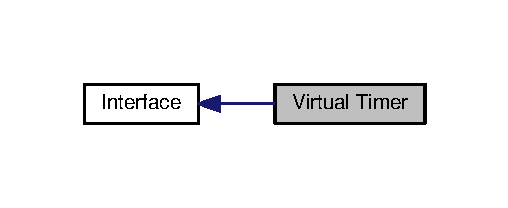
\includegraphics[width=244pt]{group__kern__vtmr}
\end{center}
\end{figure}
\subsubsection*{Data Structures}
\begin{DoxyCompactItemize}
\item 
struct \hyperlink{structesVTmr}{es\-V\-Tmr}
\begin{DoxyCompactList}\small\item\em Virtual Timer structure. \end{DoxyCompactList}\end{DoxyCompactItemize}
\subsubsection*{Typedefs}
\begin{DoxyCompactItemize}
\item 
typedef uint\-\_\-fast32\-\_\-t \hyperlink{group__kern__vtmr_ga844873888c186ee81eb66620dadb0451}{es\-Tick\-\_\-\-T}
\begin{DoxyCompactList}\small\item\em Timer tick type. \end{DoxyCompactList}\item 
typedef struct \hyperlink{structesVTmr}{es\-V\-Tmr} \hyperlink{group__kern__vtmr_ga3c020f0ca54ff412bc1d1505502d2afc}{es\-V\-Tmr\-\_\-\-T}
\begin{DoxyCompactList}\small\item\em Virtual Timer type. \end{DoxyCompactList}\end{DoxyCompactItemize}
\subsubsection*{Functions}
\begin{DoxyCompactItemize}
\item 
void \hyperlink{group__kern__vtmr_ga45fe650eac73e7fe203cc81565401555}{es\-V\-Tmr\-Init\-I} (\hyperlink{group__kern__vtmr_ga3c020f0ca54ff412bc1d1505502d2afc}{es\-V\-Tmr\-\_\-\-T} $\ast$v\-Tmr, \hyperlink{group__kern__vtmr_ga844873888c186ee81eb66620dadb0451}{es\-Tick\-\_\-\-T} tick, void($\ast$fn)(void $\ast$), void $\ast$arg)
\begin{DoxyCompactList}\small\item\em Add and start a new virtual timer. \end{DoxyCompactList}\item 
void \hyperlink{group__kern__vtmr_gad932cf00aec4ba03a0df02ccc493c4c2}{es\-V\-Tmr\-Init} (\hyperlink{group__kern__vtmr_ga3c020f0ca54ff412bc1d1505502d2afc}{es\-V\-Tmr\-\_\-\-T} $\ast$v\-Tmr, \hyperlink{group__kern__vtmr_ga844873888c186ee81eb66620dadb0451}{es\-Tick\-\_\-\-T} tick, void($\ast$fn)(void $\ast$), void $\ast$arg)
\begin{DoxyCompactList}\small\item\em Add and start a new virtual timer. \end{DoxyCompactList}\item 
void \hyperlink{group__kern__vtmr_ga96bb2c81f649c0305dfd08d1c79b2e37}{es\-V\-Tmr\-Term\-I} (\hyperlink{group__kern__vtmr_ga3c020f0ca54ff412bc1d1505502d2afc}{es\-V\-Tmr\-\_\-\-T} $\ast$v\-Tmr)
\begin{DoxyCompactList}\small\item\em Cancel and remove a virtual timer. \end{DoxyCompactList}\item 
void \hyperlink{group__kern__vtmr_gad6ec93a68e3526f18ed926cd441878cd}{es\-V\-Tmr\-Term} (\hyperlink{group__kern__vtmr_ga3c020f0ca54ff412bc1d1505502d2afc}{es\-V\-Tmr\-\_\-\-T} $\ast$v\-Tmr)
\begin{DoxyCompactList}\small\item\em Cancel and remove a virtual timer. \end{DoxyCompactList}\item 
void \hyperlink{group__kern__vtmr_ga26d10c6aaa0cd1d04261d2c9911e890d}{es\-V\-Tmr\-Delay} (\hyperlink{group__kern__vtmr_ga844873888c186ee81eb66620dadb0451}{es\-Tick\-\_\-\-T} tick)
\begin{DoxyCompactList}\small\item\em Delay for specified amount of ticks. \end{DoxyCompactList}\end{DoxyCompactItemize}


\subsubsection{Detailed Description}
Virtual Timer management services. 

\subsubsection{Typedef Documentation}
\hypertarget{group__kern__vtmr_ga844873888c186ee81eb66620dadb0451}{\index{Virtual Timer@{Virtual Timer}!es\-Tick\-\_\-\-T@{es\-Tick\-\_\-\-T}}
\index{es\-Tick\-\_\-\-T@{es\-Tick\-\_\-\-T}!Virtual Timer@{Virtual Timer}}
\paragraph[{es\-Tick\-\_\-\-T}]{\setlength{\rightskip}{0pt plus 5cm}typedef uint\-\_\-fast32\-\_\-t {\bf es\-Tick\-\_\-\-T}}}\label{group__kern__vtmr_ga844873888c186ee81eb66620dadb0451}


Timer tick type. 

\hypertarget{group__kern__vtmr_ga3c020f0ca54ff412bc1d1505502d2afc}{\index{Virtual Timer@{Virtual Timer}!es\-V\-Tmr\-\_\-\-T@{es\-V\-Tmr\-\_\-\-T}}
\index{es\-V\-Tmr\-\_\-\-T@{es\-V\-Tmr\-\_\-\-T}!Virtual Timer@{Virtual Timer}}
\paragraph[{es\-V\-Tmr\-\_\-\-T}]{\setlength{\rightskip}{0pt plus 5cm}typedef struct {\bf es\-V\-Tmr} {\bf es\-V\-Tmr\-\_\-\-T}}}\label{group__kern__vtmr_ga3c020f0ca54ff412bc1d1505502d2afc}


Virtual Timer type. 



\subsubsection{Function Documentation}
\hypertarget{group__kern__vtmr_ga45fe650eac73e7fe203cc81565401555}{\index{Virtual Timer@{Virtual Timer}!es\-V\-Tmr\-Init\-I@{es\-V\-Tmr\-Init\-I}}
\index{es\-V\-Tmr\-Init\-I@{es\-V\-Tmr\-Init\-I}!Virtual Timer@{Virtual Timer}}
\paragraph[{es\-V\-Tmr\-Init\-I}]{\setlength{\rightskip}{0pt plus 5cm}void es\-V\-Tmr\-Init\-I (
\begin{DoxyParamCaption}
\item[{{\bf es\-V\-Tmr\-\_\-\-T} $\ast$}]{v\-Tmr, }
\item[{{\bf es\-Tick\-\_\-\-T}}]{tick, }
\item[{void($\ast$)(void $\ast$)}]{fn, }
\item[{void $\ast$}]{arg}
\end{DoxyParamCaption}
)}}\label{group__kern__vtmr_ga45fe650eac73e7fe203cc81565401555}


Add and start a new virtual timer. 


\begin{DoxyParams}{Parameters}
{\em v\-Tmr} & Virtual Timer\-: is pointer to the timer I\-D structure, \hyperlink{structesVTmr}{es\-V\-Tmr}. \\
\hline
{\em tick} & Tick\-: the timer delay expressed in system ticks \\
\hline
{\em fn} & Function\-: is pointer to the callback function \\
\hline
{\em arg} & Argument\-: is pointer to the arguments of callback function \\
\hline
\end{DoxyParams}
\begin{DoxyPrecond}{Precondition}
1) {\ttfamily The kernel state $<$ E\-S\-\_\-\-K\-E\-R\-N\-\_\-\-I\-N\-A\-C\-T\-I\-V\-E}, see \hyperlink{states}{Kernel states}. 

2) {\ttfamily v\-Tmr != N\-U\-L\-L} 

3) {\ttfamily v\-Tmr-\/$>$signature != D\-E\-F\-\_\-\-V\-T\-M\-R\-\_\-\-C\-O\-N\-T\-R\-A\-C\-T\-\_\-\-S\-I\-G\-N\-A\-T\-U\-R\-E}, the timer structure can't be initialized more than once. 

4) {\ttfamily tick $>$ 1\-U} 

5) {\ttfamily fn != N\-U\-L\-L} 
\end{DoxyPrecond}
\begin{DoxyPostcond}{Postcondition}
1) {\ttfamily v\-Tmr-\/$>$signature == D\-E\-F\-\_\-\-V\-T\-M\-R\-\_\-\-C\-O\-N\-T\-R\-A\-C\-T\-\_\-\-S\-I\-G\-N\-A\-T\-U\-R\-E}, each \hyperlink{structesVTmr}{es\-V\-Tmr} structure will have valid signature after initialization. 
\end{DoxyPostcond}
\begin{DoxyNote}{Note}
The callback function is invoked from interrupt context. 
\end{DoxyNote}
\begin{DoxyParagraph}{This service can be called from\-:}

\begin{DoxyItemize}
\item Application initialization code
\item Application thread code
\item Interrupt service routine 
\end{DoxyItemize}
\end{DoxyParagraph}
\begin{DoxyParagraph}{Rescheduling\-:}

\begin{DoxyItemize}
\item never 
\end{DoxyItemize}
\end{DoxyParagraph}
\begin{DoxyParagraph}{Function class\-:}
{\bfseries I class}, Interrupt-\/lock A\-P\-I function, this function can be called only from interrupts locked code sections. 
\end{DoxyParagraph}
\hypertarget{group__kern__vtmr_gad932cf00aec4ba03a0df02ccc493c4c2}{\index{Virtual Timer@{Virtual Timer}!es\-V\-Tmr\-Init@{es\-V\-Tmr\-Init}}
\index{es\-V\-Tmr\-Init@{es\-V\-Tmr\-Init}!Virtual Timer@{Virtual Timer}}
\paragraph[{es\-V\-Tmr\-Init}]{\setlength{\rightskip}{0pt plus 5cm}void es\-V\-Tmr\-Init (
\begin{DoxyParamCaption}
\item[{{\bf es\-V\-Tmr\-\_\-\-T} $\ast$}]{v\-Tmr, }
\item[{{\bf es\-Tick\-\_\-\-T}}]{tick, }
\item[{void($\ast$)(void $\ast$)}]{fn, }
\item[{void $\ast$}]{arg}
\end{DoxyParamCaption}
)}}\label{group__kern__vtmr_gad932cf00aec4ba03a0df02ccc493c4c2}


Add and start a new virtual timer. 


\begin{DoxyParams}{Parameters}
{\em v\-Tmr} & Virtual Timer\-: is pointer to the timer I\-D structure, \hyperlink{structesVTmr}{es\-V\-Tmr}. \\
\hline
{\em tick} & Tick\-: the timer delay expressed in system ticks \\
\hline
{\em fn} & Function\-: is pointer to the callback function \\
\hline
{\em arg} & Argument\-: is pointer to the arguments of callback function \\
\hline
\end{DoxyParams}
\begin{DoxyPrecond}{Precondition}
1) {\ttfamily The kernel state $<$ E\-S\-\_\-\-K\-E\-R\-N\-\_\-\-I\-N\-A\-C\-T\-I\-V\-E}, see \hyperlink{states}{Kernel states}. 

2) {\ttfamily v\-Tmr != N\-U\-L\-L} 

3) {\ttfamily v\-Tmr-\/$>$signature != D\-E\-F\-\_\-\-V\-T\-M\-R\-\_\-\-C\-O\-N\-T\-R\-A\-C\-T\-\_\-\-S\-I\-G\-N\-A\-T\-U\-R\-E}, the timer structure can't be initialized more than once. 

4) {\ttfamily tick $>$ 1\-U} 

5) {\ttfamily fn != N\-U\-L\-L} 
\end{DoxyPrecond}
\begin{DoxyPostcond}{Postcondition}
1) {\ttfamily v\-Tmr-\/$>$signature == D\-E\-F\-\_\-\-V\-T\-M\-R\-\_\-\-C\-O\-N\-T\-R\-A\-C\-T\-\_\-\-S\-I\-G\-N\-A\-T\-U\-R\-E}, each \hyperlink{structesVTmr}{es\-V\-Tmr} structure will have valid signature after initialization. 
\end{DoxyPostcond}
\begin{DoxyNote}{Note}
The callback function is invoked from interrupt context. 
\end{DoxyNote}
\begin{DoxyParagraph}{This service can be called from\-:}

\begin{DoxyItemize}
\item Application initialization code
\item Application thread code
\item Interrupt service routine 
\end{DoxyItemize}
\end{DoxyParagraph}
\begin{DoxyParagraph}{Rescheduling\-:}

\begin{DoxyItemize}
\item never 
\end{DoxyItemize}
\end{DoxyParagraph}
\begin{DoxyParagraph}{Object class\-:}
Regular {\bfseries A\-P\-I} object, this object is part of the application programming interface. 
\end{DoxyParagraph}
\hypertarget{group__kern__vtmr_ga96bb2c81f649c0305dfd08d1c79b2e37}{\index{Virtual Timer@{Virtual Timer}!es\-V\-Tmr\-Term\-I@{es\-V\-Tmr\-Term\-I}}
\index{es\-V\-Tmr\-Term\-I@{es\-V\-Tmr\-Term\-I}!Virtual Timer@{Virtual Timer}}
\paragraph[{es\-V\-Tmr\-Term\-I}]{\setlength{\rightskip}{0pt plus 5cm}void es\-V\-Tmr\-Term\-I (
\begin{DoxyParamCaption}
\item[{{\bf es\-V\-Tmr\-\_\-\-T} $\ast$}]{v\-Tmr}
\end{DoxyParamCaption}
)}}\label{group__kern__vtmr_ga96bb2c81f649c0305dfd08d1c79b2e37}


Cancel and remove a virtual timer. 


\begin{DoxyParams}{Parameters}
{\em v\-Tmr} & Timer\-: is pointer to the timer I\-D structure, \hyperlink{structesVTmr}{es\-V\-Tmr}. \\
\hline
\end{DoxyParams}
\begin{DoxyPrecond}{Precondition}
1) {\ttfamily The kernel state $<$ E\-S\-\_\-\-K\-E\-R\-N\-\_\-\-I\-N\-A\-C\-T\-I\-V\-E}, see \hyperlink{states}{Kernel states}. 

2) {\ttfamily v\-Tmr != N\-U\-L\-L} 

3) {\ttfamily v\-Tmr-\/$>$signature == D\-E\-F\-\_\-\-V\-T\-M\-R\-\_\-\-C\-O\-N\-T\-R\-A\-C\-T\-\_\-\-S\-I\-G\-N\-A\-T\-U\-R\-E}, the pointer must point to a valid \hyperlink{structesVTmr}{es\-V\-Tmr} structure. 
\end{DoxyPrecond}
\begin{DoxyPostcond}{Postcondition}
1) {\ttfamily v\-Tmr-\/$>$signature = $\sim$\-D\-E\-F\-\_\-\-V\-T\-M\-R\-\_\-\-C\-O\-N\-T\-R\-A\-C\-T\-\_\-\-S\-I\-G\-N\-A\-T\-U\-R\-E}, each \hyperlink{structesVTmr}{es\-V\-Tmr} structure will have invalid signature after termination. 
\end{DoxyPostcond}
\begin{DoxyParagraph}{This service can be called from\-:}

\begin{DoxyItemize}
\item Application initialization code
\item Application thread code
\item Interrupt service routine 
\end{DoxyItemize}
\end{DoxyParagraph}
\begin{DoxyParagraph}{Rescheduling\-:}

\begin{DoxyItemize}
\item never 
\end{DoxyItemize}
\end{DoxyParagraph}
\begin{DoxyParagraph}{Function class\-:}
{\bfseries I class}, Interrupt-\/lock A\-P\-I function, this function can be called only from interrupts locked code sections. 
\end{DoxyParagraph}
\hypertarget{group__kern__vtmr_gad6ec93a68e3526f18ed926cd441878cd}{\index{Virtual Timer@{Virtual Timer}!es\-V\-Tmr\-Term@{es\-V\-Tmr\-Term}}
\index{es\-V\-Tmr\-Term@{es\-V\-Tmr\-Term}!Virtual Timer@{Virtual Timer}}
\paragraph[{es\-V\-Tmr\-Term}]{\setlength{\rightskip}{0pt plus 5cm}void es\-V\-Tmr\-Term (
\begin{DoxyParamCaption}
\item[{{\bf es\-V\-Tmr\-\_\-\-T} $\ast$}]{v\-Tmr}
\end{DoxyParamCaption}
)}}\label{group__kern__vtmr_gad6ec93a68e3526f18ed926cd441878cd}


Cancel and remove a virtual timer. 


\begin{DoxyParams}{Parameters}
{\em v\-Tmr} & Timer\-: is pointer to the timer I\-D structure, \hyperlink{structesVTmr}{es\-V\-Tmr}. \\
\hline
\end{DoxyParams}
\begin{DoxyPrecond}{Precondition}
1) {\ttfamily The kernel state $<$ E\-S\-\_\-\-K\-E\-R\-N\-\_\-\-I\-N\-A\-C\-T\-I\-V\-E}, see \hyperlink{states}{Kernel states}. 

2) {\ttfamily v\-Tmr != N\-U\-L\-L} 

3) {\ttfamily v\-Tmr-\/$>$signature == D\-E\-F\-\_\-\-V\-T\-M\-R\-\_\-\-C\-O\-N\-T\-R\-A\-C\-T\-\_\-\-S\-I\-G\-N\-A\-T\-U\-R\-E}, the pointer must point to a valid \hyperlink{structesVTmr}{es\-V\-Tmr} structure. 
\end{DoxyPrecond}
\begin{DoxyPostcond}{Postcondition}
1) {\ttfamily v\-Tmr-\/$>$signature = $\sim$\-D\-E\-F\-\_\-\-V\-T\-M\-R\-\_\-\-C\-O\-N\-T\-R\-A\-C\-T\-\_\-\-S\-I\-G\-N\-A\-T\-U\-R\-E}, each \hyperlink{structesVTmr}{es\-V\-Tmr} structure will have invalid signature after termination. 
\end{DoxyPostcond}
\begin{DoxyParagraph}{This service can be called from\-:}

\begin{DoxyItemize}
\item Application initialization code
\item Application thread code
\item Interrupt service routine 
\end{DoxyItemize}
\end{DoxyParagraph}
\begin{DoxyParagraph}{Rescheduling\-:}

\begin{DoxyItemize}
\item never 
\end{DoxyItemize}
\end{DoxyParagraph}
\begin{DoxyParagraph}{Object class\-:}
Regular {\bfseries A\-P\-I} object, this object is part of the application programming interface. 
\end{DoxyParagraph}
\hypertarget{group__kern__vtmr_ga26d10c6aaa0cd1d04261d2c9911e890d}{\index{Virtual Timer@{Virtual Timer}!es\-V\-Tmr\-Delay@{es\-V\-Tmr\-Delay}}
\index{es\-V\-Tmr\-Delay@{es\-V\-Tmr\-Delay}!Virtual Timer@{Virtual Timer}}
\paragraph[{es\-V\-Tmr\-Delay}]{\setlength{\rightskip}{0pt plus 5cm}void es\-V\-Tmr\-Delay (
\begin{DoxyParamCaption}
\item[{{\bf es\-Tick\-\_\-\-T}}]{tick}
\end{DoxyParamCaption}
)}}\label{group__kern__vtmr_ga26d10c6aaa0cd1d04261d2c9911e890d}


Delay for specified amount of ticks. 


\begin{DoxyParams}{Parameters}
{\em tick} & Tick\-: number of system ticks to delay.\\
\hline
\end{DoxyParams}
This function will create a virtual timer with count down time specified in argument {\ttfamily tick} and put the calling thread into {\ttfamily sleep} state. When timeout expires the thread will be placed back into {\ttfamily ready} state. \begin{DoxyNote}{Note}
The sleeping thread can not be safely awaken until the specified time does not expire. 
\end{DoxyNote}
\begin{DoxyPrecond}{Precondition}
1) {\ttfamily tick $>$ 1u} 
\end{DoxyPrecond}
\begin{DoxyParagraph}{This service can be called from\-:}

\begin{DoxyItemize}
\item Application initialization code
\item Application thread code
\item Interrupt service routine 
\end{DoxyItemize}
\end{DoxyParagraph}
\begin{DoxyParagraph}{Rescheduling\-:}

\begin{DoxyItemize}
\item always 
\end{DoxyItemize}
\end{DoxyParagraph}
\begin{DoxyParagraph}{Object class\-:}
Regular {\bfseries A\-P\-I} object, this object is part of the application programming interface. 
\end{DoxyParagraph}

\hypertarget{group__kern__ctrl}{\subsection{Kernel control block}
\label{group__kern__ctrl}\index{Kernel control block@{Kernel control block}}
}


Low-\/level kernel information and status access.  


Collaboration diagram for Kernel control block\-:\nopagebreak
\begin{figure}[H]
\begin{center}
\leavevmode
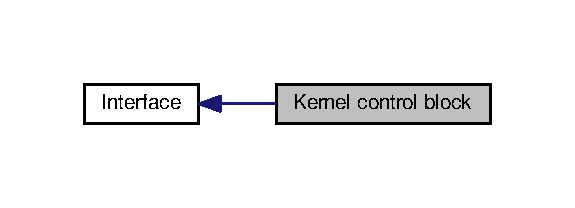
\includegraphics[width=276pt]{group__kern__ctrl}
\end{center}
\end{figure}
\subsubsection*{Data Structures}
\begin{DoxyCompactItemize}
\item 
struct \hyperlink{structkernCtrl__}{kern\-Ctrl\-\_\-}
\begin{DoxyCompactList}\small\item\em Kernel control block structure. \end{DoxyCompactList}\end{DoxyCompactItemize}
\subsubsection*{Typedefs}
\begin{DoxyCompactItemize}
\item 
typedef enum \hyperlink{group__kern__ctrl_gac9be6bfeddbd6af148cdb3867fbc24af}{es\-Kern\-State} \hyperlink{group__kern__ctrl_gab5edef44fe53303f96dc5e9f567babaf}{es\-Kern\-State\-\_\-\-T}
\begin{DoxyCompactList}\small\item\em Kernel state type. \end{DoxyCompactList}\end{DoxyCompactItemize}
\subsubsection*{Enumerations}
\begin{DoxyCompactItemize}
\item 
enum \hyperlink{group__kern__ctrl_gac9be6bfeddbd6af148cdb3867fbc24af}{es\-Kern\-State} \{ \\*
\hyperlink{group__kern__ctrl_ggac9be6bfeddbd6af148cdb3867fbc24afa31a7e1ee10bcd82aaf8f5eca06ecdbe8}{E\-S\-\_\-\-K\-E\-R\-N\-\_\-\-R\-U\-N} = 0x00u, 
\\*
\hyperlink{group__kern__ctrl_ggac9be6bfeddbd6af148cdb3867fbc24afa62e34103bea61ea0b7a9816180a43905}{E\-S\-\_\-\-K\-E\-R\-N\-\_\-\-I\-N\-T\-S\-R\-V\-\_\-\-R\-U\-N} = 0x01u, 
\\*
\hyperlink{group__kern__ctrl_ggac9be6bfeddbd6af148cdb3867fbc24afa4e5b5c809ea9cdbae536b701003278cc}{E\-S\-\_\-\-K\-E\-R\-N\-\_\-\-L\-O\-C\-K} = 0x02u, 
\\*
\hyperlink{group__kern__ctrl_ggac9be6bfeddbd6af148cdb3867fbc24afa2b35c503975df4c289e9cbff3e815f8b}{E\-S\-\_\-\-K\-E\-R\-N\-\_\-\-I\-N\-T\-S\-R\-V\-\_\-\-L\-O\-C\-K} = 0x03u, 
\\*
\hyperlink{group__kern__ctrl_ggac9be6bfeddbd6af148cdb3867fbc24afad45a94c8b4975fd162d683201a75cceb}{E\-S\-\_\-\-K\-E\-R\-N\-\_\-\-S\-L\-E\-E\-P} = 0x06u, 
\\*
\hyperlink{group__kern__ctrl_ggac9be6bfeddbd6af148cdb3867fbc24afacad35dc43528f96d27696db584f05cff}{E\-S\-\_\-\-K\-E\-R\-N\-\_\-\-I\-N\-I\-T} = 0x08u, 
\\*
\hyperlink{group__kern__ctrl_ggac9be6bfeddbd6af148cdb3867fbc24afa089165cac55f315953335f5ffe41b7c4}{E\-S\-\_\-\-K\-E\-R\-N\-\_\-\-I\-N\-A\-C\-T\-I\-V\-E} = 0x10u
 \}
\begin{DoxyCompactList}\small\item\em Kernel state enumeration. \end{DoxyCompactList}\end{DoxyCompactItemize}
\subsubsection*{Variables}
\begin{DoxyCompactItemize}
\item 
const struct \hyperlink{structkernCtrl__}{kern\-Ctrl\-\_\-} \hyperlink{group__kern__ctrl_ga93a7ee7768ffd94201bf1795a543194b}{Kern\-Ctrl}
\begin{DoxyCompactList}\small\item\em Kernel control block. \end{DoxyCompactList}\end{DoxyCompactItemize}


\subsubsection{Detailed Description}
Low-\/level kernel information and status access. 

\subsubsection{Typedef Documentation}
\hypertarget{group__kern__ctrl_gab5edef44fe53303f96dc5e9f567babaf}{\index{Kernel control block@{Kernel control block}!es\-Kern\-State\-\_\-\-T@{es\-Kern\-State\-\_\-\-T}}
\index{es\-Kern\-State\-\_\-\-T@{es\-Kern\-State\-\_\-\-T}!Kernel control block@{Kernel control block}}
\paragraph[{es\-Kern\-State\-\_\-\-T}]{\setlength{\rightskip}{0pt plus 5cm}typedef enum {\bf es\-Kern\-State} {\bf es\-Kern\-State\-\_\-\-T}}}\label{group__kern__ctrl_gab5edef44fe53303f96dc5e9f567babaf}


Kernel state type. 



\subsubsection{Enumeration Type Documentation}
\hypertarget{group__kern__ctrl_gac9be6bfeddbd6af148cdb3867fbc24af}{\index{Kernel control block@{Kernel control block}!es\-Kern\-State@{es\-Kern\-State}}
\index{es\-Kern\-State@{es\-Kern\-State}!Kernel control block@{Kernel control block}}
\paragraph[{es\-Kern\-State}]{\setlength{\rightskip}{0pt plus 5cm}enum {\bf es\-Kern\-State}}}\label{group__kern__ctrl_gac9be6bfeddbd6af148cdb3867fbc24af}


Kernel state enumeration. 

For more details see\-: \hyperlink{states}{Kernel states} \begin{DoxyParagraph}{Object class\-:}
Regular {\bfseries A\-P\-I} object, this object is part of the application programming interface. 
\end{DoxyParagraph}
\begin{Desc}
\item[Enumerator]\par
\begin{description}
\index{E\-S\-\_\-\-K\-E\-R\-N\-\_\-\-R\-U\-N@{E\-S\-\_\-\-K\-E\-R\-N\-\_\-\-R\-U\-N}!Kernel control block@{Kernel control block}}\index{Kernel control block@{Kernel control block}!E\-S\-\_\-\-K\-E\-R\-N\-\_\-\-R\-U\-N@{E\-S\-\_\-\-K\-E\-R\-N\-\_\-\-R\-U\-N}}\item[{\em 
\hypertarget{group__kern__ctrl_ggac9be6bfeddbd6af148cdb3867fbc24afa31a7e1ee10bcd82aaf8f5eca06ecdbe8}{E\-S\-\_\-\-K\-E\-R\-N\-\_\-\-R\-U\-N}\label{group__kern__ctrl_ggac9be6bfeddbd6af148cdb3867fbc24afa31a7e1ee10bcd82aaf8f5eca06ecdbe8}
}]Kernel is active \index{E\-S\-\_\-\-K\-E\-R\-N\-\_\-\-I\-N\-T\-S\-R\-V\-\_\-\-R\-U\-N@{E\-S\-\_\-\-K\-E\-R\-N\-\_\-\-I\-N\-T\-S\-R\-V\-\_\-\-R\-U\-N}!Kernel control block@{Kernel control block}}\index{Kernel control block@{Kernel control block}!E\-S\-\_\-\-K\-E\-R\-N\-\_\-\-I\-N\-T\-S\-R\-V\-\_\-\-R\-U\-N@{E\-S\-\_\-\-K\-E\-R\-N\-\_\-\-I\-N\-T\-S\-R\-V\-\_\-\-R\-U\-N}}\item[{\em 
\hypertarget{group__kern__ctrl_ggac9be6bfeddbd6af148cdb3867fbc24afa62e34103bea61ea0b7a9816180a43905}{E\-S\-\_\-\-K\-E\-R\-N\-\_\-\-I\-N\-T\-S\-R\-V\-\_\-\-R\-U\-N}\label{group__kern__ctrl_ggac9be6bfeddbd6af148cdb3867fbc24afa62e34103bea61ea0b7a9816180a43905}
}]Servicing an interrupt, return to E\-S\-\_\-\-K\-E\-R\-N\-\_\-\-R\-U\-N state \index{E\-S\-\_\-\-K\-E\-R\-N\-\_\-\-L\-O\-C\-K@{E\-S\-\_\-\-K\-E\-R\-N\-\_\-\-L\-O\-C\-K}!Kernel control block@{Kernel control block}}\index{Kernel control block@{Kernel control block}!E\-S\-\_\-\-K\-E\-R\-N\-\_\-\-L\-O\-C\-K@{E\-S\-\_\-\-K\-E\-R\-N\-\_\-\-L\-O\-C\-K}}\item[{\em 
\hypertarget{group__kern__ctrl_ggac9be6bfeddbd6af148cdb3867fbc24afa4e5b5c809ea9cdbae536b701003278cc}{E\-S\-\_\-\-K\-E\-R\-N\-\_\-\-L\-O\-C\-K}\label{group__kern__ctrl_ggac9be6bfeddbd6af148cdb3867fbc24afa4e5b5c809ea9cdbae536b701003278cc}
}]Kernel is locked \index{E\-S\-\_\-\-K\-E\-R\-N\-\_\-\-I\-N\-T\-S\-R\-V\-\_\-\-L\-O\-C\-K@{E\-S\-\_\-\-K\-E\-R\-N\-\_\-\-I\-N\-T\-S\-R\-V\-\_\-\-L\-O\-C\-K}!Kernel control block@{Kernel control block}}\index{Kernel control block@{Kernel control block}!E\-S\-\_\-\-K\-E\-R\-N\-\_\-\-I\-N\-T\-S\-R\-V\-\_\-\-L\-O\-C\-K@{E\-S\-\_\-\-K\-E\-R\-N\-\_\-\-I\-N\-T\-S\-R\-V\-\_\-\-L\-O\-C\-K}}\item[{\em 
\hypertarget{group__kern__ctrl_ggac9be6bfeddbd6af148cdb3867fbc24afa2b35c503975df4c289e9cbff3e815f8b}{E\-S\-\_\-\-K\-E\-R\-N\-\_\-\-I\-N\-T\-S\-R\-V\-\_\-\-L\-O\-C\-K}\label{group__kern__ctrl_ggac9be6bfeddbd6af148cdb3867fbc24afa2b35c503975df4c289e9cbff3e815f8b}
}]Servicing an interrupt, return to E\-S\-\_\-\-K\-E\-R\-N\-\_\-\-L\-O\-C\-K state \index{E\-S\-\_\-\-K\-E\-R\-N\-\_\-\-S\-L\-E\-E\-P@{E\-S\-\_\-\-K\-E\-R\-N\-\_\-\-S\-L\-E\-E\-P}!Kernel control block@{Kernel control block}}\index{Kernel control block@{Kernel control block}!E\-S\-\_\-\-K\-E\-R\-N\-\_\-\-S\-L\-E\-E\-P@{E\-S\-\_\-\-K\-E\-R\-N\-\_\-\-S\-L\-E\-E\-P}}\item[{\em 
\hypertarget{group__kern__ctrl_ggac9be6bfeddbd6af148cdb3867fbc24afad45a94c8b4975fd162d683201a75cceb}{E\-S\-\_\-\-K\-E\-R\-N\-\_\-\-S\-L\-E\-E\-P}\label{group__kern__ctrl_ggac9be6bfeddbd6af148cdb3867fbc24afad45a94c8b4975fd162d683201a75cceb}
}]Kernel is sleeping \index{E\-S\-\_\-\-K\-E\-R\-N\-\_\-\-I\-N\-I\-T@{E\-S\-\_\-\-K\-E\-R\-N\-\_\-\-I\-N\-I\-T}!Kernel control block@{Kernel control block}}\index{Kernel control block@{Kernel control block}!E\-S\-\_\-\-K\-E\-R\-N\-\_\-\-I\-N\-I\-T@{E\-S\-\_\-\-K\-E\-R\-N\-\_\-\-I\-N\-I\-T}}\item[{\em 
\hypertarget{group__kern__ctrl_ggac9be6bfeddbd6af148cdb3867fbc24afacad35dc43528f96d27696db584f05cff}{E\-S\-\_\-\-K\-E\-R\-N\-\_\-\-I\-N\-I\-T}\label{group__kern__ctrl_ggac9be6bfeddbd6af148cdb3867fbc24afacad35dc43528f96d27696db584f05cff}
}]Kernel is in initialization state \index{E\-S\-\_\-\-K\-E\-R\-N\-\_\-\-I\-N\-A\-C\-T\-I\-V\-E@{E\-S\-\_\-\-K\-E\-R\-N\-\_\-\-I\-N\-A\-C\-T\-I\-V\-E}!Kernel control block@{Kernel control block}}\index{Kernel control block@{Kernel control block}!E\-S\-\_\-\-K\-E\-R\-N\-\_\-\-I\-N\-A\-C\-T\-I\-V\-E@{E\-S\-\_\-\-K\-E\-R\-N\-\_\-\-I\-N\-A\-C\-T\-I\-V\-E}}\item[{\em 
\hypertarget{group__kern__ctrl_ggac9be6bfeddbd6af148cdb3867fbc24afa089165cac55f315953335f5ffe41b7c4}{E\-S\-\_\-\-K\-E\-R\-N\-\_\-\-I\-N\-A\-C\-T\-I\-V\-E}\label{group__kern__ctrl_ggac9be6bfeddbd6af148cdb3867fbc24afa089165cac55f315953335f5ffe41b7c4}
}]Kernel data structures are not initialized \end{description}
\end{Desc}


\subsubsection{Variable Documentation}
\hypertarget{group__kern__ctrl_ga93a7ee7768ffd94201bf1795a543194b}{\index{Kernel control block@{Kernel control block}!Kern\-Ctrl@{Kern\-Ctrl}}
\index{Kern\-Ctrl@{Kern\-Ctrl}!Kernel control block@{Kernel control block}}
\paragraph[{Kern\-Ctrl}]{\setlength{\rightskip}{0pt plus 5cm}const struct {\bf kern\-Ctrl\-\_\-} Kern\-Ctrl}}\label{group__kern__ctrl_ga93a7ee7768ffd94201bf1795a543194b}


Kernel control block. 

\begin{DoxyNote}{Note}
This variable has Read-\/\-Only access rights for application.
\end{DoxyNote}
Kernel control block. 
\hypertarget{group__kern__lock}{\subsection{Kernel lock}
\label{group__kern__lock}\index{Kernel lock@{Kernel lock}}
}


Kernel lock management.  


Collaboration diagram for Kernel lock\-:\nopagebreak
\begin{figure}[H]
\begin{center}
\leavevmode
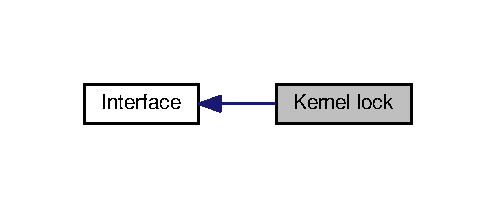
\includegraphics[width=238pt]{group__kern__lock}
\end{center}
\end{figure}
\subsubsection*{Typedefs}
\begin{DoxyCompactItemize}
\item 
typedef port\-Reg\-\_\-\-T \hyperlink{group__kern__lock_gad8b2b8257c3bf42c064adb66c0d45e2e}{es\-Lock\-Ctx\-\_\-\-T}
\begin{DoxyCompactList}\small\item\em Kernel lock context type. \end{DoxyCompactList}\end{DoxyCompactItemize}
\subsubsection*{Functions}
\begin{DoxyCompactItemize}
\item 
void \hyperlink{group__kern__lock_gaa3ca4a02fafcfb840442506f42175a13}{es\-Kern\-Lock\-Int\-Enter} (\hyperlink{group__kern__lock_gad8b2b8257c3bf42c064adb66c0d45e2e}{es\-Lock\-Ctx\-\_\-\-T} $\ast$lock\-Ctx)
\begin{DoxyCompactList}\small\item\em Enter a critical code lock. \end{DoxyCompactList}\item 
void \hyperlink{group__kern__lock_gad8cb192a48802804cc12162edd18668d}{es\-Kern\-Lock\-Int\-Exit} (\hyperlink{group__kern__lock_gad8b2b8257c3bf42c064adb66c0d45e2e}{es\-Lock\-Ctx\-\_\-\-T} lock\-Ctx)
\begin{DoxyCompactList}\small\item\em Exit a critical code lock. \end{DoxyCompactList}\item 
void \hyperlink{group__kern__lock_ga6dd45355c20a10f7272bd39670353428}{es\-Kern\-Lock\-Enter\-I} (void)
\begin{DoxyCompactList}\small\item\em Lock the scheduler. \end{DoxyCompactList}\item 
void \hyperlink{group__kern__lock_ga3287aefb2c7dd24672c716d86a008ad3}{es\-Kern\-Lock\-Exit\-I} (void)
\begin{DoxyCompactList}\small\item\em Unlock the scheduler. \end{DoxyCompactList}\item 
void \hyperlink{group__kern__lock_ga86ec4f4cbaa889b0f23c7e2ebdcbbb97}{es\-Kern\-Lock\-Enter} (void)
\begin{DoxyCompactList}\small\item\em Lock the scheduler. \end{DoxyCompactList}\item 
void \hyperlink{group__kern__lock_gaf1eec663f7cc5c414b113901382ccd82}{es\-Kern\-Lock\-Exit} (void)
\begin{DoxyCompactList}\small\item\em Unlock the scheduler. \end{DoxyCompactList}\end{DoxyCompactItemize}


\subsubsection{Detailed Description}
Kernel lock management. These methods provide the most basic mechanism to protect concurrent access to a shared resource.

For more details see \hyperlink{critical_section}{Critical sections}. 

\subsubsection{Typedef Documentation}
\hypertarget{group__kern__lock_gad8b2b8257c3bf42c064adb66c0d45e2e}{\index{Kernel lock@{Kernel lock}!es\-Lock\-Ctx\-\_\-\-T@{es\-Lock\-Ctx\-\_\-\-T}}
\index{es\-Lock\-Ctx\-\_\-\-T@{es\-Lock\-Ctx\-\_\-\-T}!Kernel lock@{Kernel lock}}
\paragraph[{es\-Lock\-Ctx\-\_\-\-T}]{\setlength{\rightskip}{0pt plus 5cm}typedef port\-Reg\-\_\-\-T {\bf es\-Lock\-Ctx\-\_\-\-T}}}\label{group__kern__lock_gad8b2b8257c3bf42c064adb66c0d45e2e}


Kernel lock context type. 

Variables declared using this type can hold current lock context which can be restored after a critical code section is exited. 

\subsubsection{Function Documentation}
\hypertarget{group__kern__lock_gaa3ca4a02fafcfb840442506f42175a13}{\index{Kernel lock@{Kernel lock}!es\-Kern\-Lock\-Int\-Enter@{es\-Kern\-Lock\-Int\-Enter}}
\index{es\-Kern\-Lock\-Int\-Enter@{es\-Kern\-Lock\-Int\-Enter}!Kernel lock@{Kernel lock}}
\paragraph[{es\-Kern\-Lock\-Int\-Enter}]{\setlength{\rightskip}{0pt plus 5cm}void es\-Kern\-Lock\-Int\-Enter (
\begin{DoxyParamCaption}
\item[{{\bf es\-Lock\-Ctx\-\_\-\-T} $\ast$}]{lock\-Ctx}
\end{DoxyParamCaption}
)}}\label{group__kern__lock_gaa3ca4a02fafcfb840442506f42175a13}


Enter a critical code lock. 


\begin{DoxyParams}{Parameters}
{\em lock\-Ctx} & Pointer to context variable where to store the current lock context. \\
\hline
\end{DoxyParams}
\begin{DoxyParagraph}{This service can be called from\-:}

\begin{DoxyItemize}
\item Application initialization code
\item Application thread code 
\end{DoxyItemize}
\end{DoxyParagraph}
\begin{DoxyParagraph}{Rescheduling\-:}

\begin{DoxyItemize}
\item never 
\end{DoxyItemize}
\end{DoxyParagraph}
\begin{DoxyParagraph}{Object class\-:}
Regular {\bfseries A\-P\-I} object, this object is part of the application programming interface. 
\end{DoxyParagraph}
\hypertarget{group__kern__lock_gad8cb192a48802804cc12162edd18668d}{\index{Kernel lock@{Kernel lock}!es\-Kern\-Lock\-Int\-Exit@{es\-Kern\-Lock\-Int\-Exit}}
\index{es\-Kern\-Lock\-Int\-Exit@{es\-Kern\-Lock\-Int\-Exit}!Kernel lock@{Kernel lock}}
\paragraph[{es\-Kern\-Lock\-Int\-Exit}]{\setlength{\rightskip}{0pt plus 5cm}void es\-Kern\-Lock\-Int\-Exit (
\begin{DoxyParamCaption}
\item[{{\bf es\-Lock\-Ctx\-\_\-\-T}}]{lock\-Ctx}
\end{DoxyParamCaption}
)}}\label{group__kern__lock_gad8cb192a48802804cc12162edd18668d}


Exit a critical code lock. 


\begin{DoxyParams}{Parameters}
{\em lock\-Ctx} & Context variable value\\
\hline
\end{DoxyParams}
Restores the lock context to state before the \hyperlink{group__kern__lock_gaa3ca4a02fafcfb840442506f42175a13}{es\-Kern\-Lock\-Int\-Enter()} was called. \begin{DoxyParagraph}{This service can be called from\-:}

\begin{DoxyItemize}
\item Application initialization code
\item Application thread code 
\end{DoxyItemize}
\end{DoxyParagraph}
\begin{DoxyParagraph}{Rescheduling\-:}

\begin{DoxyItemize}
\item possible 
\end{DoxyItemize}
\end{DoxyParagraph}
\begin{DoxyParagraph}{Object class\-:}
Regular {\bfseries A\-P\-I} object, this object is part of the application programming interface. 
\end{DoxyParagraph}
\hypertarget{group__kern__lock_ga6dd45355c20a10f7272bd39670353428}{\index{Kernel lock@{Kernel lock}!es\-Kern\-Lock\-Enter\-I@{es\-Kern\-Lock\-Enter\-I}}
\index{es\-Kern\-Lock\-Enter\-I@{es\-Kern\-Lock\-Enter\-I}!Kernel lock@{Kernel lock}}
\paragraph[{es\-Kern\-Lock\-Enter\-I}]{\setlength{\rightskip}{0pt plus 5cm}void es\-Kern\-Lock\-Enter\-I (
\begin{DoxyParamCaption}
\item[{void}]{}
\end{DoxyParamCaption}
)}}\label{group__kern__lock_ga6dd45355c20a10f7272bd39670353428}


Lock the scheduler. 

\begin{DoxyPrecond}{Precondition}
1) {\ttfamily The kernel state $<$ E\-S\-\_\-\-K\-E\-R\-N\-\_\-\-I\-N\-I\-T}, see \hyperlink{states}{Kernel states}. 
\end{DoxyPrecond}
\begin{DoxyParagraph}{This service can be called from\-:}

\begin{DoxyItemize}
\item Application thread code 
\end{DoxyItemize}
\end{DoxyParagraph}
\begin{DoxyParagraph}{Rescheduling\-:}

\begin{DoxyItemize}
\item never 
\end{DoxyItemize}
\end{DoxyParagraph}
\begin{DoxyParagraph}{Function class\-:}
{\bfseries I class}, Interrupt-\/lock A\-P\-I function, this function can be called only from interrupts locked code sections. 
\end{DoxyParagraph}
\hypertarget{group__kern__lock_ga3287aefb2c7dd24672c716d86a008ad3}{\index{Kernel lock@{Kernel lock}!es\-Kern\-Lock\-Exit\-I@{es\-Kern\-Lock\-Exit\-I}}
\index{es\-Kern\-Lock\-Exit\-I@{es\-Kern\-Lock\-Exit\-I}!Kernel lock@{Kernel lock}}
\paragraph[{es\-Kern\-Lock\-Exit\-I}]{\setlength{\rightskip}{0pt plus 5cm}void es\-Kern\-Lock\-Exit\-I (
\begin{DoxyParamCaption}
\item[{void}]{}
\end{DoxyParamCaption}
)}}\label{group__kern__lock_ga3287aefb2c7dd24672c716d86a008ad3}


Unlock the scheduler. 

\begin{DoxyPrecond}{Precondition}
1) {\ttfamily The kernel state $<$ E\-S\-\_\-\-K\-E\-R\-N\-\_\-\-I\-N\-I\-T}, see \hyperlink{states}{Kernel states}. 

2) {\ttfamily g\-Kern\-Lock\-Cnt $>$ 0u}, current number of locks must be greater than zero, in other words\-: each call to kernel lock function must have its matching call to kernel unlock function. 
\end{DoxyPrecond}
\begin{DoxyParagraph}{This service can be called from\-:}

\begin{DoxyItemize}
\item Application thread code 
\end{DoxyItemize}
\end{DoxyParagraph}
\begin{DoxyParagraph}{Rescheduling\-:}

\begin{DoxyItemize}
\item possible 
\end{DoxyItemize}
\end{DoxyParagraph}
\begin{DoxyParagraph}{Function class\-:}
{\bfseries I class}, Interrupt-\/lock A\-P\-I function, this function can be called only from interrupts locked code sections. 
\end{DoxyParagraph}
\hypertarget{group__kern__lock_ga86ec4f4cbaa889b0f23c7e2ebdcbbb97}{\index{Kernel lock@{Kernel lock}!es\-Kern\-Lock\-Enter@{es\-Kern\-Lock\-Enter}}
\index{es\-Kern\-Lock\-Enter@{es\-Kern\-Lock\-Enter}!Kernel lock@{Kernel lock}}
\paragraph[{es\-Kern\-Lock\-Enter}]{\setlength{\rightskip}{0pt plus 5cm}void es\-Kern\-Lock\-Enter (
\begin{DoxyParamCaption}
\item[{void}]{}
\end{DoxyParamCaption}
)}}\label{group__kern__lock_ga86ec4f4cbaa889b0f23c7e2ebdcbbb97}


Lock the scheduler. 

\begin{DoxyPrecond}{Precondition}
1) {\ttfamily The kernel state $<$ E\-S\-\_\-\-K\-E\-R\-N\-\_\-\-I\-N\-I\-T}, see \hyperlink{states}{Kernel states}. 
\end{DoxyPrecond}
\begin{DoxyParagraph}{This service can be called from\-:}

\begin{DoxyItemize}
\item Application thread code 
\end{DoxyItemize}
\end{DoxyParagraph}
\begin{DoxyParagraph}{Rescheduling\-:}

\begin{DoxyItemize}
\item never 
\end{DoxyItemize}
\end{DoxyParagraph}
\begin{DoxyParagraph}{Object class\-:}
Regular {\bfseries A\-P\-I} object, this object is part of the application programming interface. 
\end{DoxyParagraph}
\hypertarget{group__kern__lock_gaf1eec663f7cc5c414b113901382ccd82}{\index{Kernel lock@{Kernel lock}!es\-Kern\-Lock\-Exit@{es\-Kern\-Lock\-Exit}}
\index{es\-Kern\-Lock\-Exit@{es\-Kern\-Lock\-Exit}!Kernel lock@{Kernel lock}}
\paragraph[{es\-Kern\-Lock\-Exit}]{\setlength{\rightskip}{0pt plus 5cm}void es\-Kern\-Lock\-Exit (
\begin{DoxyParamCaption}
\item[{void}]{}
\end{DoxyParamCaption}
)}}\label{group__kern__lock_gaf1eec663f7cc5c414b113901382ccd82}


Unlock the scheduler. 

\begin{DoxyPrecond}{Precondition}
1) {\ttfamily The kernel state $<$ E\-S\-\_\-\-K\-E\-R\-N\-\_\-\-I\-N\-I\-T}, see \hyperlink{states}{Kernel states}. 

2) {\ttfamily g\-Kern\-Lock\-Cnt $>$ 0u}, current number of locks must be greater than zero, in other words\-: each call to kernel lock function must have its matching call to kernel unlock function. 
\end{DoxyPrecond}
\begin{DoxyParagraph}{This service can be called from\-:}

\begin{DoxyItemize}
\item Application thread code 
\end{DoxyItemize}
\end{DoxyParagraph}
\begin{DoxyParagraph}{Rescheduling\-:}

\begin{DoxyItemize}
\item possible 
\end{DoxyItemize}
\end{DoxyParagraph}
\begin{DoxyParagraph}{Object class\-:}
Regular {\bfseries A\-P\-I} object, this object is part of the application programming interface. 
\end{DoxyParagraph}

\hypertarget{group__kern__general}{\subsection{General kernel functions}
\label{group__kern__general}\index{General kernel functions@{General kernel functions}}
}


Kernel initialization, start-\/up, I\-S\-R management.  


Collaboration diagram for General kernel functions\-:\nopagebreak
\begin{figure}[H]
\begin{center}
\leavevmode
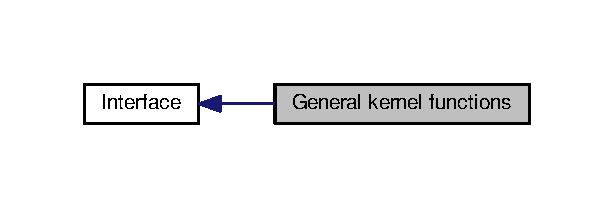
\includegraphics[width=294pt]{group__kern__general}
\end{center}
\end{figure}
\subsubsection*{Functions}
\begin{DoxyCompactItemize}
\item 
void \hyperlink{group__kern__general_ga9e9ff699d62d6035cd51121bb3140704}{es\-Kern\-Init} (void)
\begin{DoxyCompactList}\small\item\em Initialize kernel internal data structures. \end{DoxyCompactList}\item 
P\-O\-R\-T\-\_\-\-C\-\_\-\-N\-O\-R\-E\-T\-U\-R\-N void \hyperlink{group__kern__general_ga0e7a0a6b9c02df58de0f98de0229a09d}{es\-Kern\-Start} (void)
\begin{DoxyCompactList}\small\item\em Start the multi-\/threading. \end{DoxyCompactList}\item 
void \hyperlink{group__kern__general_ga3182e4c1a47897109d0a429b10a2483e}{es\-Kern\-Sys\-Tmr} (void)
\begin{DoxyCompactList}\small\item\em Process the system timer event. \end{DoxyCompactList}\item 
void \hyperlink{group__kern__general_gac0d578bcd4a10b2c8e5fc90f0b86ccec}{es\-Kern\-Isr\-Enter\-I} (void)
\begin{DoxyCompactList}\small\item\em Enter Interrupt Service Routine. \end{DoxyCompactList}\item 
void \hyperlink{group__kern__general_gaa6347925fff1684b5425dd2857c27129}{es\-Kern\-Isr\-Exit\-I} (void)
\begin{DoxyCompactList}\small\item\em Exit Interrupt Service Routine. \end{DoxyCompactList}\end{DoxyCompactItemize}


\subsubsection{Detailed Description}
Kernel initialization, start-\/up, I\-S\-R management. There are several groups of functions\-:
\begin{DoxyItemize}
\item kernel initialization and start
\item I\-S\-R enter and exit 
\end{DoxyItemize}

\subsubsection{Function Documentation}
\hypertarget{group__kern__general_ga9e9ff699d62d6035cd51121bb3140704}{\index{General kernel functions@{General kernel functions}!es\-Kern\-Init@{es\-Kern\-Init}}
\index{es\-Kern\-Init@{es\-Kern\-Init}!General kernel functions@{General kernel functions}}
\paragraph[{es\-Kern\-Init}]{\setlength{\rightskip}{0pt plus 5cm}void es\-Kern\-Init (
\begin{DoxyParamCaption}
\item[{void}]{}
\end{DoxyParamCaption}
)}}\label{group__kern__general_ga9e9ff699d62d6035cd51121bb3140704}


Initialize kernel internal data structures. 

\begin{DoxyPrecond}{Precondition}
1) {\ttfamily The kernel state == E\-S\-\_\-\-K\-E\-R\-N\-\_\-\-I\-N\-A\-C\-T\-I\-V\-E}, see \hyperlink{states}{Kernel states}. 
\end{DoxyPrecond}
\begin{DoxyPostcond}{Postcondition}
1) {\ttfamily The kernel state == E\-S\-\_\-\-K\-E\-R\-N\-\_\-\-I\-N\-I\-T}. 
\end{DoxyPostcond}
\begin{DoxyNote}{Note}
1) This function may be invoked only once.
\end{DoxyNote}
This function must be called first before any other kernel A\-P\-I. It initializes internal data structures that are used by other A\-P\-I functions. \begin{DoxyParagraph}{This service can be called from\-:}

\begin{DoxyItemize}
\item Application initialization code 
\end{DoxyItemize}
\end{DoxyParagraph}
\begin{DoxyParagraph}{Rescheduling\-:}

\begin{DoxyItemize}
\item never 
\end{DoxyItemize}
\end{DoxyParagraph}
\begin{DoxyParagraph}{Object class\-:}
Regular {\bfseries A\-P\-I} object, this object is part of the application programming interface. 
\end{DoxyParagraph}
\hypertarget{group__kern__general_ga0e7a0a6b9c02df58de0f98de0229a09d}{\index{General kernel functions@{General kernel functions}!es\-Kern\-Start@{es\-Kern\-Start}}
\index{es\-Kern\-Start@{es\-Kern\-Start}!General kernel functions@{General kernel functions}}
\paragraph[{es\-Kern\-Start}]{\setlength{\rightskip}{0pt plus 5cm}P\-O\-R\-T\-\_\-\-C\-\_\-\-N\-O\-R\-E\-T\-U\-R\-N void es\-Kern\-Start (
\begin{DoxyParamCaption}
\item[{void}]{}
\end{DoxyParamCaption}
)}}\label{group__kern__general_ga0e7a0a6b9c02df58de0f98de0229a09d}


Start the multi-\/threading. 

\begin{DoxyPrecond}{Precondition}
1) {\ttfamily The kernel state == E\-S\-\_\-\-K\-E\-R\-N\-\_\-\-I\-N\-I\-T}, see \hyperlink{states}{Kernel states}. 
\end{DoxyPrecond}
\begin{DoxyPostcond}{Postcondition}
1) {\ttfamily The kernel state == E\-S\-\_\-\-K\-E\-R\-N\-\_\-\-R\-U\-N} 

2) The multi-\/threading execution will commence. 
\end{DoxyPostcond}
\begin{DoxyNote}{Note}
1) Once this function is called the execution of threads will start and this function will never return.
\end{DoxyNote}
This function will start multi-\/threading. Once the multi-\/threading has started the execution will never return to this function again (this function never returns). \begin{DoxyParagraph}{This service can be called from\-:}

\begin{DoxyItemize}
\item Application initialization code 
\end{DoxyItemize}
\end{DoxyParagraph}
\begin{DoxyParagraph}{Rescheduling\-:}

\begin{DoxyItemize}
\item always 
\end{DoxyItemize}
\end{DoxyParagraph}
\begin{DoxyParagraph}{Object class\-:}
Regular {\bfseries A\-P\-I} object, this object is part of the application programming interface. 
\end{DoxyParagraph}
\hypertarget{group__kern__general_ga3182e4c1a47897109d0a429b10a2483e}{\index{General kernel functions@{General kernel functions}!es\-Kern\-Sys\-Tmr@{es\-Kern\-Sys\-Tmr}}
\index{es\-Kern\-Sys\-Tmr@{es\-Kern\-Sys\-Tmr}!General kernel functions@{General kernel functions}}
\paragraph[{es\-Kern\-Sys\-Tmr}]{\setlength{\rightskip}{0pt plus 5cm}void es\-Kern\-Sys\-Tmr (
\begin{DoxyParamCaption}
\item[{void}]{}
\end{DoxyParamCaption}
)}}\label{group__kern__general_ga3182e4c1a47897109d0a429b10a2483e}


Process the system timer event. 

\begin{DoxyPrecond}{Precondition}
1) {\ttfamily The kernel state $<$ E\-S\-\_\-\-K\-E\-R\-N\-\_\-\-I\-N\-I\-T}, see \hyperlink{states}{Kernel states}.
\end{DoxyPrecond}
This function will be called only by port system timer interrupt. \begin{DoxyParagraph}{Object class\-:}
{\bfseries Not A\-P\-I} object, this object is not part of the application programming interface and it is intended for internal use only. 
\end{DoxyParagraph}
\hypertarget{group__kern__general_gac0d578bcd4a10b2c8e5fc90f0b86ccec}{\index{General kernel functions@{General kernel functions}!es\-Kern\-Isr\-Enter\-I@{es\-Kern\-Isr\-Enter\-I}}
\index{es\-Kern\-Isr\-Enter\-I@{es\-Kern\-Isr\-Enter\-I}!General kernel functions@{General kernel functions}}
\paragraph[{es\-Kern\-Isr\-Enter\-I}]{\setlength{\rightskip}{0pt plus 5cm}void es\-Kern\-Isr\-Enter\-I (
\begin{DoxyParamCaption}
\item[{void}]{}
\end{DoxyParamCaption}
)}}\label{group__kern__general_gac0d578bcd4a10b2c8e5fc90f0b86ccec}


Enter Interrupt Service Routine. 

\begin{DoxyPrecond}{Precondition}
1) {\ttfamily The kernel state $<$ E\-S\-\_\-\-K\-E\-R\-N\-\_\-\-I\-N\-I\-T}, see \hyperlink{states}{Kernel states}. 
\end{DoxyPrecond}
\begin{DoxyNote}{Note}
1) You must call \hyperlink{group__kern__general_gaa6347925fff1684b5425dd2857c27129}{es\-Kern\-Isr\-Exit\-I()} at the exit of I\-S\-R. 

2) You must invoke \hyperlink{group__kern__general_gac0d578bcd4a10b2c8e5fc90f0b86ccec}{es\-Kern\-Isr\-Enter\-I()} and \hyperlink{group__kern__general_gaa6347925fff1684b5425dd2857c27129}{es\-Kern\-Isr\-Exit\-I()} in pair. In other words, for every call to \hyperlink{group__kern__general_gac0d578bcd4a10b2c8e5fc90f0b86ccec}{es\-Kern\-Isr\-Enter\-I()} at the beginning of the I\-S\-R you must have a call to \hyperlink{group__kern__general_gaa6347925fff1684b5425dd2857c27129}{es\-Kern\-Isr\-Exit\-I()} at the end of the I\-S\-R.
\end{DoxyNote}
Function will notify kernel that you are about to enter interrupt service routine (I\-S\-R). This allows kernel to keep track of interrupt nesting and then only perform rescheduling at the last nested I\-S\-R. \begin{DoxyParagraph}{This service can be called from\-:}

\begin{DoxyItemize}
\item Interrupt service routine 
\end{DoxyItemize}
\end{DoxyParagraph}
\begin{DoxyParagraph}{Rescheduling\-:}

\begin{DoxyItemize}
\item never 
\end{DoxyItemize}
\end{DoxyParagraph}
\begin{DoxyParagraph}{Function class\-:}
{\bfseries I class}, Interrupt-\/lock A\-P\-I function, this function can be called only from interrupts locked code sections. 
\end{DoxyParagraph}
\hypertarget{group__kern__general_gaa6347925fff1684b5425dd2857c27129}{\index{General kernel functions@{General kernel functions}!es\-Kern\-Isr\-Exit\-I@{es\-Kern\-Isr\-Exit\-I}}
\index{es\-Kern\-Isr\-Exit\-I@{es\-Kern\-Isr\-Exit\-I}!General kernel functions@{General kernel functions}}
\paragraph[{es\-Kern\-Isr\-Exit\-I}]{\setlength{\rightskip}{0pt plus 5cm}void es\-Kern\-Isr\-Exit\-I (
\begin{DoxyParamCaption}
\item[{void}]{}
\end{DoxyParamCaption}
)}}\label{group__kern__general_gaa6347925fff1684b5425dd2857c27129}


Exit Interrupt Service Routine. 

\begin{DoxyPrecond}{Precondition}
1) {\ttfamily The kernel state $<$ E\-S\-\_\-\-K\-E\-R\-N\-\_\-\-I\-N\-I\-T}, see \hyperlink{states}{Kernel states}. 
\end{DoxyPrecond}
\begin{DoxyNote}{Note}
1) You must invoke \hyperlink{group__kern__general_gac0d578bcd4a10b2c8e5fc90f0b86ccec}{es\-Kern\-Isr\-Enter\-I()} and \hyperlink{group__kern__general_gaa6347925fff1684b5425dd2857c27129}{es\-Kern\-Isr\-Exit\-I()} in pair. In other words, for every call to \hyperlink{group__kern__general_gac0d578bcd4a10b2c8e5fc90f0b86ccec}{es\-Kern\-Isr\-Enter\-I()} at the beginning of the I\-S\-R you must have a call to \hyperlink{group__kern__general_gaa6347925fff1684b5425dd2857c27129}{es\-Kern\-Isr\-Exit\-I()} at the end of the I\-S\-R. 

2) Rescheduling is prevented when the scheduler is locked (see \hyperlink{group__kern__lock_ga6dd45355c20a10f7272bd39670353428}{es\-Kern\-Lock\-Enter\-I()})
\end{DoxyNote}
This function is used to notify kernel that you have completed servicing an interrupt. When the last nested I\-S\-R has completed, the function will call the scheduler to determine whether a new, high-\/priority task, is ready to run. \begin{DoxyParagraph}{This service can be called from\-:}

\begin{DoxyItemize}
\item Interrupt service routine 
\end{DoxyItemize}
\end{DoxyParagraph}
\begin{DoxyParagraph}{Rescheduling\-:}

\begin{DoxyItemize}
\item possible 
\end{DoxyItemize}
\end{DoxyParagraph}
\begin{DoxyParagraph}{Function class\-:}
{\bfseries I class}, Interrupt-\/lock A\-P\-I function, this function can be called only from interrupts locked code sections. 
\end{DoxyParagraph}

\hypertarget{group__kern__sched}{\subsection{Scheduler notification and invocation}
\label{group__kern__sched}\index{Scheduler notification and invocation@{Scheduler notification and invocation}}
}


Low-\/level scheduler services.  


Collaboration diagram for Scheduler notification and invocation\-:\nopagebreak
\begin{figure}[H]
\begin{center}
\leavevmode
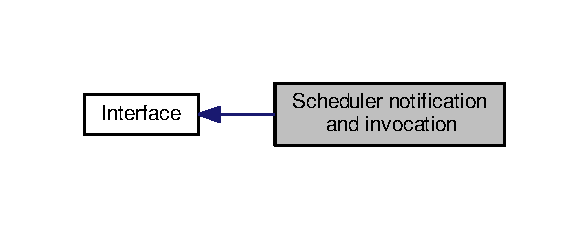
\includegraphics[width=282pt]{group__kern__sched}
\end{center}
\end{figure}
\subsubsection*{Functions}
\begin{DoxyCompactItemize}
\item 
void \hyperlink{group__kern__sched_ga73e14b1860ce824c822adc407aee0977}{es\-Sched\-Rdy\-Add\-I} (\hyperlink{group__kern__thd_ga62e3a3ca0a4597a19c43cb8868810d82}{es\-Thd\-\_\-\-T} $\ast$thd)
\begin{DoxyCompactList}\small\item\em Add thread {\ttfamily thd} to the ready thread list and notify the scheduler. \end{DoxyCompactList}\item 
void \hyperlink{group__kern__sched_ga0b8263c5024ebb59cd9b95cc9253b44d}{es\-Sched\-Rdy\-Rm\-I} (\hyperlink{group__kern__thd_ga62e3a3ca0a4597a19c43cb8868810d82}{es\-Thd\-\_\-\-T} $\ast$thd)
\begin{DoxyCompactList}\small\item\em Remove thread {\ttfamily thd} from the ready thread list and notify the scheduler. \end{DoxyCompactList}\item 
void \hyperlink{group__kern__sched_gaf90e487bfce974dafaeed5009e189810}{es\-Sched\-Yield\-I} (void)
\begin{DoxyCompactList}\small\item\em Force the scheduler invocation which will evaluate all ready threads and switch to ready thread with the highest priority. \end{DoxyCompactList}\item 
void \hyperlink{group__kern__sched_gafbea29b376b29f11bbfc48a0f5144e9a}{es\-Sched\-Yield\-Isr\-I} (void)
\begin{DoxyCompactList}\small\item\em Force the scheduler invocation which will evaluate all ready threads and switch to ready thread with the highest priority. \end{DoxyCompactList}\end{DoxyCompactItemize}


\subsubsection{Detailed Description}
Low-\/level scheduler services. 

\subsubsection{Function Documentation}
\hypertarget{group__kern__sched_ga73e14b1860ce824c822adc407aee0977}{\index{Scheduler notification and invocation@{Scheduler notification and invocation}!es\-Sched\-Rdy\-Add\-I@{es\-Sched\-Rdy\-Add\-I}}
\index{es\-Sched\-Rdy\-Add\-I@{es\-Sched\-Rdy\-Add\-I}!Scheduler notification and invocation@{Scheduler notification and invocation}}
\paragraph[{es\-Sched\-Rdy\-Add\-I}]{\setlength{\rightskip}{0pt plus 5cm}void es\-Sched\-Rdy\-Add\-I (
\begin{DoxyParamCaption}
\item[{{\bf es\-Thd\-\_\-\-T} $\ast$}]{thd}
\end{DoxyParamCaption}
)}}\label{group__kern__sched_ga73e14b1860ce824c822adc407aee0977}


Add thread {\ttfamily thd} to the ready thread list and notify the scheduler. 


\begin{DoxyParams}{Parameters}
{\em thd} & Pointer to the initialized thread I\-D structure, \hyperlink{structesThd}{es\-Thd}. \\
\hline
\end{DoxyParams}
\begin{DoxyPrecond}{Precondition}
1) {\ttfamily The kernel state $<$ E\-S\-\_\-\-K\-E\-R\-N\-\_\-\-I\-N\-A\-C\-T\-I\-V\-E}, see \hyperlink{states}{Kernel states}. 

2) {\ttfamily thd != N\-U\-L\-L} 

3) {\ttfamily thd-\/$>$signature == D\-E\-F\-\_\-\-T\-H\-D\-\_\-\-C\-O\-N\-T\-R\-A\-C\-T\-\_\-\-S\-I\-G\-N\-A\-T\-U\-R\-E}, the pointer must point to a valid \hyperlink{structesThd}{es\-Thd} structure. 

4) {\ttfamily thd-\/$>$thd\-L\-\_\-.\-q == N\-U\-L\-L}, thread must not be in a queue. 
\end{DoxyPrecond}
\begin{DoxyParagraph}{This service can be called from\-:}

\begin{DoxyItemize}
\item Application initialization code
\item Application thread code
\item Interrupt service routine 
\end{DoxyItemize}
\end{DoxyParagraph}
\begin{DoxyParagraph}{Rescheduling\-:}

\begin{DoxyItemize}
\item never 
\end{DoxyItemize}
\end{DoxyParagraph}
\begin{DoxyParagraph}{Function class\-:}
{\bfseries I class}, Interrupt-\/lock A\-P\-I function, this function can be called only from interrupts locked code sections. 
\end{DoxyParagraph}
\hypertarget{group__kern__sched_ga0b8263c5024ebb59cd9b95cc9253b44d}{\index{Scheduler notification and invocation@{Scheduler notification and invocation}!es\-Sched\-Rdy\-Rm\-I@{es\-Sched\-Rdy\-Rm\-I}}
\index{es\-Sched\-Rdy\-Rm\-I@{es\-Sched\-Rdy\-Rm\-I}!Scheduler notification and invocation@{Scheduler notification and invocation}}
\paragraph[{es\-Sched\-Rdy\-Rm\-I}]{\setlength{\rightskip}{0pt plus 5cm}void es\-Sched\-Rdy\-Rm\-I (
\begin{DoxyParamCaption}
\item[{{\bf es\-Thd\-\_\-\-T} $\ast$}]{thd}
\end{DoxyParamCaption}
)}}\label{group__kern__sched_ga0b8263c5024ebb59cd9b95cc9253b44d}


Remove thread {\ttfamily thd} from the ready thread list and notify the scheduler. 


\begin{DoxyParams}{Parameters}
{\em thd} & Pointer to the initialized thread I\-D structure, \hyperlink{structesThd}{es\-Thd}. \\
\hline
\end{DoxyParams}
\begin{DoxyPrecond}{Precondition}
1) {\ttfamily The kernel state $<$ E\-S\-\_\-\-K\-E\-R\-N\-\_\-\-I\-N\-A\-C\-T\-I\-V\-E}, see \hyperlink{states}{Kernel states}. 

2) {\ttfamily thd != N\-U\-L\-L} 

3) {\ttfamily thd-\/$>$signature == D\-E\-F\-\_\-\-T\-H\-D\-\_\-\-C\-O\-N\-T\-R\-A\-C\-T\-\_\-\-S\-I\-G\-N\-A\-T\-U\-R\-E}, the pointer must point to a valid \hyperlink{structesThd}{es\-Thd} structure. 

4) {\ttfamily thd-\/$>$thd\-L\-\_\-.\-q == \&g\-Rdy\-Queue}, thread must be in Ready Threads queue. 
\end{DoxyPrecond}
\begin{DoxyParagraph}{This service can be called from\-:}

\begin{DoxyItemize}
\item Application initialization code
\item Application thread code
\item Interrupt service routine 
\end{DoxyItemize}
\end{DoxyParagraph}
\begin{DoxyParagraph}{Rescheduling\-:}

\begin{DoxyItemize}
\item never 
\end{DoxyItemize}
\end{DoxyParagraph}
\begin{DoxyParagraph}{Function class\-:}
{\bfseries I class}, Interrupt-\/lock A\-P\-I function, this function can be called only from interrupts locked code sections. 
\end{DoxyParagraph}
\hypertarget{group__kern__sched_gaf90e487bfce974dafaeed5009e189810}{\index{Scheduler notification and invocation@{Scheduler notification and invocation}!es\-Sched\-Yield\-I@{es\-Sched\-Yield\-I}}
\index{es\-Sched\-Yield\-I@{es\-Sched\-Yield\-I}!Scheduler notification and invocation@{Scheduler notification and invocation}}
\paragraph[{es\-Sched\-Yield\-I}]{\setlength{\rightskip}{0pt plus 5cm}void es\-Sched\-Yield\-I (
\begin{DoxyParamCaption}
\item[{void}]{}
\end{DoxyParamCaption}
)}}\label{group__kern__sched_gaf90e487bfce974dafaeed5009e189810}


Force the scheduler invocation which will evaluate all ready threads and switch to ready thread with the highest priority. 

\begin{DoxyPrecond}{Precondition}
1) {\ttfamily The kernel state $<$ E\-S\-\_\-\-K\-E\-R\-N\-\_\-\-I\-N\-A\-C\-T\-I\-V\-E}, see \hyperlink{states}{Kernel states}. 
\end{DoxyPrecond}
\begin{DoxyParagraph}{This service can be called from\-:}

\begin{DoxyItemize}
\item Application thread code 
\end{DoxyItemize}
\end{DoxyParagraph}
\begin{DoxyParagraph}{Rescheduling\-:}

\begin{DoxyItemize}
\item possible 
\end{DoxyItemize}
\end{DoxyParagraph}
\begin{DoxyParagraph}{Function class\-:}
{\bfseries I class}, Interrupt-\/lock A\-P\-I function, this function can be called only from interrupts locked code sections. 
\end{DoxyParagraph}
\hypertarget{group__kern__sched_gafbea29b376b29f11bbfc48a0f5144e9a}{\index{Scheduler notification and invocation@{Scheduler notification and invocation}!es\-Sched\-Yield\-Isr\-I@{es\-Sched\-Yield\-Isr\-I}}
\index{es\-Sched\-Yield\-Isr\-I@{es\-Sched\-Yield\-Isr\-I}!Scheduler notification and invocation@{Scheduler notification and invocation}}
\paragraph[{es\-Sched\-Yield\-Isr\-I}]{\setlength{\rightskip}{0pt plus 5cm}void es\-Sched\-Yield\-Isr\-I (
\begin{DoxyParamCaption}
\item[{void}]{}
\end{DoxyParamCaption}
)}}\label{group__kern__sched_gafbea29b376b29f11bbfc48a0f5144e9a}


Force the scheduler invocation which will evaluate all ready threads and switch to ready thread with the highest priority. 

\begin{DoxyPrecond}{Precondition}
1) {\ttfamily The kernel state $<$ E\-S\-\_\-\-K\-E\-R\-N\-\_\-\-I\-N\-A\-C\-T\-I\-V\-E}, see \hyperlink{states}{Kernel states}. 
\end{DoxyPrecond}
\begin{DoxyParagraph}{This service can be called from\-:}

\begin{DoxyItemize}
\item Interrupt service routine 
\end{DoxyItemize}
\end{DoxyParagraph}
\begin{DoxyParagraph}{Rescheduling\-:}

\begin{DoxyItemize}
\item possible 
\end{DoxyItemize}
\end{DoxyParagraph}
\begin{DoxyParagraph}{Function class\-:}
{\bfseries I class}, Interrupt-\/lock A\-P\-I function, this function can be called only from interrupts locked code sections. 
\end{DoxyParagraph}

\hypertarget{group__kern__time}{\subsection{Kernel time}
\label{group__kern__time}\index{Kernel time@{Kernel time}}
}


Kernel time management.  


Collaboration diagram for Kernel time\-:\nopagebreak
\begin{figure}[H]
\begin{center}
\leavevmode
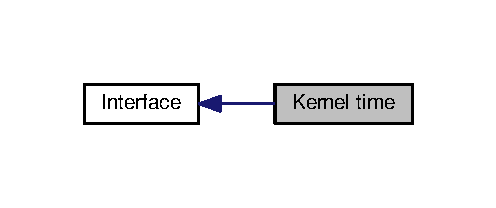
\includegraphics[width=238pt]{group__kern__time}
\end{center}
\end{figure}
\subsubsection*{Functions}
\begin{DoxyCompactItemize}
\item 
\hyperlink{group__kern__vtmr_ga844873888c186ee81eb66620dadb0451}{es\-Tick\-\_\-\-T} \hyperlink{group__kern__time_gacb0d88d6a7e467dc37a6a9a85945aaa6}{es\-Sys\-Tmr\-Tick\-Get} (void)
\begin{DoxyCompactList}\small\item\em Get the current tick value. \end{DoxyCompactList}\end{DoxyCompactItemize}


\subsubsection{Detailed Description}
Kernel time management. 

\subsubsection{Function Documentation}
\hypertarget{group__kern__time_gacb0d88d6a7e467dc37a6a9a85945aaa6}{\index{Kernel time@{Kernel time}!es\-Sys\-Tmr\-Tick\-Get@{es\-Sys\-Tmr\-Tick\-Get}}
\index{es\-Sys\-Tmr\-Tick\-Get@{es\-Sys\-Tmr\-Tick\-Get}!Kernel time@{Kernel time}}
\paragraph[{es\-Sys\-Tmr\-Tick\-Get}]{\setlength{\rightskip}{0pt plus 5cm}{\bf es\-Tick\-\_\-\-T} es\-Sys\-Tmr\-Tick\-Get (
\begin{DoxyParamCaption}
\item[{void}]{}
\end{DoxyParamCaption}
)}}\label{group__kern__time_gacb0d88d6a7e467dc37a6a9a85945aaa6}


Get the current tick value. 

\begin{DoxyReturn}{Returns}
Current tick value 
\end{DoxyReturn}
\begin{DoxyPrecond}{Precondition}
1) {\ttfamily The kernel state $<$ E\-S\-\_\-\-K\-E\-R\-N\-\_\-\-I\-N\-A\-C\-T\-I\-V\-E}, see \hyperlink{states}{Kernel states}. 
\end{DoxyPrecond}
\begin{DoxyParagraph}{This service can be called from\-:}

\begin{DoxyItemize}
\item Application initialization code
\item Application thread code
\item Interrupt service routine 
\end{DoxyItemize}
\end{DoxyParagraph}
\begin{DoxyParagraph}{Rescheduling\-:}

\begin{DoxyItemize}
\item never 
\end{DoxyItemize}
\end{DoxyParagraph}
\begin{DoxyParagraph}{Object class\-:}
Regular {\bfseries A\-P\-I} object, this object is part of the application programming interface. 
\end{DoxyParagraph}

\hypertarget{group__kern__hook}{\subsection{Kernel hook functions}
\label{group__kern__hook}\index{Kernel hook functions@{Kernel hook functions}}
}


User defined hook (callback) function prototypes.  


Collaboration diagram for Kernel hook functions\-:\nopagebreak
\begin{figure}[H]
\begin{center}
\leavevmode
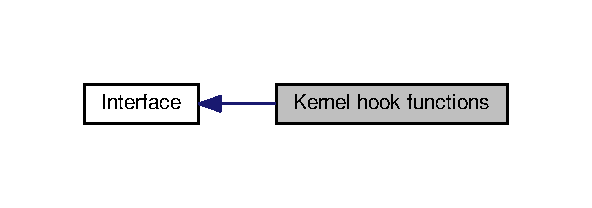
\includegraphics[width=284pt]{group__kern__hook}
\end{center}
\end{figure}
\subsubsection*{Functions}
\begin{DoxyCompactItemize}
\item 
void \hyperlink{group__kern__hook_ga9a0d562969acef0121136b11be7b4728}{user\-Pre\-Sys\-Tmr} (void)
\begin{DoxyCompactList}\small\item\em System timer hook function, called from system system timer I\-S\-R function before the kernel functions. \end{DoxyCompactList}\item 
void \hyperlink{group__kern__hook_gaac77966856c9a299cda4794cbcc87edf}{user\-Pre\-Kern\-Init} (void)
\begin{DoxyCompactList}\small\item\em Kernel initialization hook function, called from \hyperlink{group__kern__general_ga9e9ff699d62d6035cd51121bb3140704}{es\-Kern\-Init()} function before kernel initialization. \end{DoxyCompactList}\item 
void \hyperlink{group__kern__hook_ga3579ac6964a314ad03d13da0507f57e8}{user\-Post\-Kern\-Init} (void)
\begin{DoxyCompactList}\small\item\em Kernel initialization hook function, called from \hyperlink{group__kern__general_ga9e9ff699d62d6035cd51121bb3140704}{es\-Kern\-Init()} function after kernel initialization. \end{DoxyCompactList}\item 
void \hyperlink{group__kern__hook_gaac505ab4c72e0fb346ca441d6def327d}{user\-Pre\-Kern\-Start} (void)
\begin{DoxyCompactList}\small\item\em Kernel start hook function, called from \hyperlink{group__kern__general_ga0e7a0a6b9c02df58de0f98de0229a09d}{es\-Kern\-Start()} function. \end{DoxyCompactList}\item 
void \hyperlink{group__kern__hook_ga64ca864d0ff2aaa532208d7c2b88bdb3}{user\-Post\-Thd\-Init} (\hyperlink{group__kern__thd_ga62e3a3ca0a4597a19c43cb8868810d82}{es\-Thd\-\_\-\-T} $\ast$thd)
\begin{DoxyCompactList}\small\item\em Thread initialization end hook function, called from \hyperlink{group__kern__thd_gac91734f3ee867b519f59bf81cc7fde88}{es\-Thd\-Init()} function. \end{DoxyCompactList}\item 
void \hyperlink{group__kern__hook_ga076ad76633999c9d5e245e3b5c6e0c09}{user\-Pre\-Thd\-Term} (void)
\begin{DoxyCompactList}\small\item\em Thread terminate hook function, called from \hyperlink{group__kern__thd_gac9d1eac76f26096614e8196bcfd8b905}{es\-Thd\-Term()} or when a thread terminates itself. \end{DoxyCompactList}\item 
void \hyperlink{group__kern__hook_ga2bd40d82f768787c3dab2f4df336685e}{user\-Pre\-Idle} (void)
\begin{DoxyCompactList}\small\item\em Pre Idle hook function, called from idle thread, just before entering idle period. \end{DoxyCompactList}\item 
void \hyperlink{group__kern__hook_ga7ca4a96cbe5064d633298d1d172fd4e7}{user\-Post\-Idle} (void)
\begin{DoxyCompactList}\small\item\em Post idle hook function, called from idle thread, just after exiting idle period. \end{DoxyCompactList}\item 
void \hyperlink{group__kern__hook_ga74a38c965110d0f2f2e44e13571fe3fc}{user\-Pre\-Ctx\-Sw} (\hyperlink{group__kern__thd_ga62e3a3ca0a4597a19c43cb8868810d82}{es\-Thd\-\_\-\-T} $\ast$old\-Thd, \hyperlink{group__kern__thd_ga62e3a3ca0a4597a19c43cb8868810d82}{es\-Thd\-\_\-\-T} $\ast$new\-Thd)
\begin{DoxyCompactList}\small\item\em Kernel context switch hook function, called from \hyperlink{group__kern__sched_gaf90e487bfce974dafaeed5009e189810}{es\-Sched\-Yield\-I()} and \hyperlink{group__kern__sched_gafbea29b376b29f11bbfc48a0f5144e9a}{es\-Sched\-Yield\-Isr\-I()} functions just before context switch. \end{DoxyCompactList}\end{DoxyCompactItemize}


\subsubsection{Detailed Description}
User defined hook (callback) function prototypes. \begin{DoxyNote}{Note}
1) The definition of this functions must be written by the user. 
\end{DoxyNote}


\subsubsection{Function Documentation}
\hypertarget{group__kern__hook_ga9a0d562969acef0121136b11be7b4728}{\index{Kernel hook functions@{Kernel hook functions}!user\-Pre\-Sys\-Tmr@{user\-Pre\-Sys\-Tmr}}
\index{user\-Pre\-Sys\-Tmr@{user\-Pre\-Sys\-Tmr}!Kernel hook functions@{Kernel hook functions}}
\paragraph[{user\-Pre\-Sys\-Tmr}]{\setlength{\rightskip}{0pt plus 5cm}void user\-Pre\-Sys\-Tmr (
\begin{DoxyParamCaption}
\item[{void}]{}
\end{DoxyParamCaption}
)}}\label{group__kern__hook_ga9a0d562969acef0121136b11be7b4728}


System timer hook function, called from system system timer I\-S\-R function before the kernel functions. 

\begin{DoxyNote}{Note}
1) This function is called only if \hyperlink{group__template__kern__cfg_gaa130bc9f72010b44b4b06618d8f8d0bc}{C\-F\-G\-\_\-\-H\-O\-O\-K\-\_\-\-P\-R\-E\-\_\-\-S\-Y\-S\-T\-M\-R\-\_\-\-E\-V\-E\-N\-T} is active.
\end{DoxyNote}
This function is called whenever a system event is generated. \hypertarget{group__kern__hook_gaac77966856c9a299cda4794cbcc87edf}{\index{Kernel hook functions@{Kernel hook functions}!user\-Pre\-Kern\-Init@{user\-Pre\-Kern\-Init}}
\index{user\-Pre\-Kern\-Init@{user\-Pre\-Kern\-Init}!Kernel hook functions@{Kernel hook functions}}
\paragraph[{user\-Pre\-Kern\-Init}]{\setlength{\rightskip}{0pt plus 5cm}void user\-Pre\-Kern\-Init (
\begin{DoxyParamCaption}
\item[{void}]{}
\end{DoxyParamCaption}
)}}\label{group__kern__hook_gaac77966856c9a299cda4794cbcc87edf}


Kernel initialization hook function, called from \hyperlink{group__kern__general_ga9e9ff699d62d6035cd51121bb3140704}{es\-Kern\-Init()} function before kernel initialization. 

\begin{DoxyNote}{Note}
1) This function is called only if \hyperlink{group__template__kern__cfg_ga4093113f2105d2716f86c6509a6e643a}{C\-F\-G\-\_\-\-H\-O\-O\-K\-\_\-\-P\-R\-E\-\_\-\-K\-E\-R\-N\-\_\-\-I\-N\-I\-T} is active.
\end{DoxyNote}
This function is called before the kernel initialization. \hypertarget{group__kern__hook_ga3579ac6964a314ad03d13da0507f57e8}{\index{Kernel hook functions@{Kernel hook functions}!user\-Post\-Kern\-Init@{user\-Post\-Kern\-Init}}
\index{user\-Post\-Kern\-Init@{user\-Post\-Kern\-Init}!Kernel hook functions@{Kernel hook functions}}
\paragraph[{user\-Post\-Kern\-Init}]{\setlength{\rightskip}{0pt plus 5cm}void user\-Post\-Kern\-Init (
\begin{DoxyParamCaption}
\item[{void}]{}
\end{DoxyParamCaption}
)}}\label{group__kern__hook_ga3579ac6964a314ad03d13da0507f57e8}


Kernel initialization hook function, called from \hyperlink{group__kern__general_ga9e9ff699d62d6035cd51121bb3140704}{es\-Kern\-Init()} function after kernel initialization. 

\begin{DoxyNote}{Note}
1) This function is called only if \hyperlink{group__template__kern__cfg_ga85dea823714335c2ec9e9f7750996e83}{C\-F\-G\-\_\-\-H\-O\-O\-K\-\_\-\-P\-O\-S\-T\-\_\-\-K\-E\-R\-N\-\_\-\-I\-N\-I\-T} is active.
\end{DoxyNote}
This function is called after the kernel initialization. \hypertarget{group__kern__hook_gaac505ab4c72e0fb346ca441d6def327d}{\index{Kernel hook functions@{Kernel hook functions}!user\-Pre\-Kern\-Start@{user\-Pre\-Kern\-Start}}
\index{user\-Pre\-Kern\-Start@{user\-Pre\-Kern\-Start}!Kernel hook functions@{Kernel hook functions}}
\paragraph[{user\-Pre\-Kern\-Start}]{\setlength{\rightskip}{0pt plus 5cm}void user\-Pre\-Kern\-Start (
\begin{DoxyParamCaption}
\item[{void}]{}
\end{DoxyParamCaption}
)}}\label{group__kern__hook_gaac505ab4c72e0fb346ca441d6def327d}


Kernel start hook function, called from \hyperlink{group__kern__general_ga0e7a0a6b9c02df58de0f98de0229a09d}{es\-Kern\-Start()} function. 

\begin{DoxyNote}{Note}
1) This function is called only if \hyperlink{group__template__kern__cfg_gad67d998118375811b0f3e63543311661}{C\-F\-G\-\_\-\-H\-O\-O\-K\-\_\-\-P\-R\-E\-\_\-\-K\-E\-R\-N\-\_\-\-S\-T\-A\-R\-T} is active.
\end{DoxyNote}
This function is called before kernel start. \hypertarget{group__kern__hook_ga64ca864d0ff2aaa532208d7c2b88bdb3}{\index{Kernel hook functions@{Kernel hook functions}!user\-Post\-Thd\-Init@{user\-Post\-Thd\-Init}}
\index{user\-Post\-Thd\-Init@{user\-Post\-Thd\-Init}!Kernel hook functions@{Kernel hook functions}}
\paragraph[{user\-Post\-Thd\-Init}]{\setlength{\rightskip}{0pt plus 5cm}void user\-Post\-Thd\-Init (
\begin{DoxyParamCaption}
\item[{{\bf es\-Thd\-\_\-\-T} $\ast$}]{thd}
\end{DoxyParamCaption}
)}}\label{group__kern__hook_ga64ca864d0ff2aaa532208d7c2b88bdb3}


Thread initialization end hook function, called from \hyperlink{group__kern__thd_gac91734f3ee867b519f59bf81cc7fde88}{es\-Thd\-Init()} function. 


\begin{DoxyParams}{Parameters}
{\em thd} & Thread\-: pointer to thread Id structure that has just been initialized. \\
\hline
\end{DoxyParams}
\begin{DoxyNote}{Note}
1) This function is called only if \hyperlink{group__template__kern__cfg_ga23deae306171d1a8dda4d0e33efdb6bb}{C\-F\-G\-\_\-\-H\-O\-O\-K\-\_\-\-P\-O\-S\-T\-\_\-\-T\-H\-D\-\_\-\-I\-N\-I\-T} is active.
\end{DoxyNote}
This function is called after the thread initialization. \hypertarget{group__kern__hook_ga076ad76633999c9d5e245e3b5c6e0c09}{\index{Kernel hook functions@{Kernel hook functions}!user\-Pre\-Thd\-Term@{user\-Pre\-Thd\-Term}}
\index{user\-Pre\-Thd\-Term@{user\-Pre\-Thd\-Term}!Kernel hook functions@{Kernel hook functions}}
\paragraph[{user\-Pre\-Thd\-Term}]{\setlength{\rightskip}{0pt plus 5cm}void user\-Pre\-Thd\-Term (
\begin{DoxyParamCaption}
\item[{void}]{}
\end{DoxyParamCaption}
)}}\label{group__kern__hook_ga076ad76633999c9d5e245e3b5c6e0c09}


Thread terminate hook function, called from \hyperlink{group__kern__thd_gac9d1eac76f26096614e8196bcfd8b905}{es\-Thd\-Term()} or when a thread terminates itself. 

\begin{DoxyNote}{Note}
1) This function is called only if \hyperlink{group__template__kern__cfg_ga9c7dd4e009a89e9cffb0f9b404bc6250}{C\-F\-G\-\_\-\-H\-O\-O\-K\-\_\-\-P\-R\-E\-\_\-\-T\-H\-D\-\_\-\-T\-E\-R\-M} is active. 
\end{DoxyNote}
\hypertarget{group__kern__hook_ga2bd40d82f768787c3dab2f4df336685e}{\index{Kernel hook functions@{Kernel hook functions}!user\-Pre\-Idle@{user\-Pre\-Idle}}
\index{user\-Pre\-Idle@{user\-Pre\-Idle}!Kernel hook functions@{Kernel hook functions}}
\paragraph[{user\-Pre\-Idle}]{\setlength{\rightskip}{0pt plus 5cm}void user\-Pre\-Idle (
\begin{DoxyParamCaption}
\item[{void}]{}
\end{DoxyParamCaption}
)}}\label{group__kern__hook_ga2bd40d82f768787c3dab2f4df336685e}


Pre Idle hook function, called from idle thread, just before entering idle period. 

\begin{DoxyNote}{Note}
1) This function is called only if \hyperlink{group__template__kern__cfg_ga7c2b0410404256c4804758090401f7e4}{C\-F\-G\-\_\-\-H\-O\-O\-K\-\_\-\-P\-R\-E\-\_\-\-I\-D\-L\-E} and \hyperlink{group__template__kern__cfg_ga4e6ab4994b34501bb71e75717b093376}{C\-F\-G\-\_\-\-S\-C\-H\-E\-D\-\_\-\-P\-O\-W\-E\-R\-\_\-\-S\-A\-V\-E} are active. 

2) This function is called with interrupts and scheduler locked. 
\end{DoxyNote}
\hypertarget{group__kern__hook_ga7ca4a96cbe5064d633298d1d172fd4e7}{\index{Kernel hook functions@{Kernel hook functions}!user\-Post\-Idle@{user\-Post\-Idle}}
\index{user\-Post\-Idle@{user\-Post\-Idle}!Kernel hook functions@{Kernel hook functions}}
\paragraph[{user\-Post\-Idle}]{\setlength{\rightskip}{0pt plus 5cm}void user\-Post\-Idle (
\begin{DoxyParamCaption}
\item[{void}]{}
\end{DoxyParamCaption}
)}}\label{group__kern__hook_ga7ca4a96cbe5064d633298d1d172fd4e7}


Post idle hook function, called from idle thread, just after exiting idle period. 

\begin{DoxyNote}{Note}
1) This function is called only if \hyperlink{group__template__kern__cfg_ga8f8751efe94964bef25673deca6b9b26}{C\-F\-G\-\_\-\-H\-O\-O\-K\-\_\-\-P\-O\-S\-T\-\_\-\-I\-D\-L\-E} and \hyperlink{group__template__kern__cfg_ga4e6ab4994b34501bb71e75717b093376}{C\-F\-G\-\_\-\-S\-C\-H\-E\-D\-\_\-\-P\-O\-W\-E\-R\-\_\-\-S\-A\-V\-E} are active. 

2) This function is called with scheduler locked. 
\end{DoxyNote}
\hypertarget{group__kern__hook_ga74a38c965110d0f2f2e44e13571fe3fc}{\index{Kernel hook functions@{Kernel hook functions}!user\-Pre\-Ctx\-Sw@{user\-Pre\-Ctx\-Sw}}
\index{user\-Pre\-Ctx\-Sw@{user\-Pre\-Ctx\-Sw}!Kernel hook functions@{Kernel hook functions}}
\paragraph[{user\-Pre\-Ctx\-Sw}]{\setlength{\rightskip}{0pt plus 5cm}void user\-Pre\-Ctx\-Sw (
\begin{DoxyParamCaption}
\item[{{\bf es\-Thd\-\_\-\-T} $\ast$}]{old\-Thd, }
\item[{{\bf es\-Thd\-\_\-\-T} $\ast$}]{new\-Thd}
\end{DoxyParamCaption}
)}}\label{group__kern__hook_ga74a38c965110d0f2f2e44e13571fe3fc}


Kernel context switch hook function, called from \hyperlink{group__kern__sched_gaf90e487bfce974dafaeed5009e189810}{es\-Sched\-Yield\-I()} and \hyperlink{group__kern__sched_gafbea29b376b29f11bbfc48a0f5144e9a}{es\-Sched\-Yield\-Isr\-I()} functions just before context switch. 


\begin{DoxyParams}{Parameters}
{\em old\-Thd} & Pointer to the thread being switched out. \\
\hline
{\em new\-Thd} & Pointer to the thread being switched in. \\
\hline
\end{DoxyParams}
\begin{DoxyNote}{Note}
1) This function is called only if \hyperlink{group__template__kern__cfg_gac84acbf84222018398089920dd429635}{C\-F\-G\-\_\-\-H\-O\-O\-K\-\_\-\-P\-R\-E\-\_\-\-C\-T\-X\-\_\-\-S\-W} is active.
\end{DoxyNote}
This function is called at each context switch. 
\hypertarget{group__kern__impl}{\subsection{Internals}
\label{group__kern__impl}\index{Internals@{Internals}}
}


Kernel inner work.  


Collaboration diagram for Internals\-:\nopagebreak
\begin{figure}[H]
\begin{center}
\leavevmode
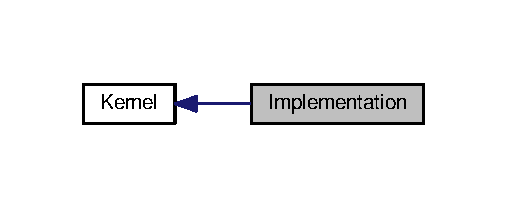
\includegraphics[width=214pt]{group__kern__impl}
\end{center}
\end{figure}
\subsubsection*{Data Structures}
\begin{DoxyCompactItemize}
\item 
struct \hyperlink{structsysTmr}{sys\-Tmr}
\begin{DoxyCompactList}\small\item\em Main System Timer structure. \end{DoxyCompactList}\end{DoxyCompactItemize}
\subsubsection*{Macros}
\begin{DoxyCompactItemize}
\item 
\#define \hyperlink{group__kern__impl_ga4a1ac440197aa9f2d77edf92c5b3b83c}{P\-R\-I\-O\-\_\-\-B\-M\-\_\-\-D\-A\-T\-A\-\_\-\-W\-I\-D\-T\-H\-\_\-\-L\-O\-G2}
\begin{DoxyCompactList}\small\item\em Priority Bit Map log base 2\-: {\ttfamily log2(\-P\-O\-R\-T\-\_\-\-D\-E\-F\-\_\-\-D\-A\-T\-A\-\_\-\-W\-I\-D\-T\-H)} \end{DoxyCompactList}\item 
\#define \hyperlink{group__kern__impl_ga11143896be344ab4dd20f6eb690918e7}{S\-C\-H\-E\-D\-\_\-\-S\-T\-A\-T\-E\-\_\-\-I\-N\-T\-S\-R\-V\-\_\-\-M\-S\-K}~(1u $<$$<$ 0)
\begin{DoxyCompactList}\small\item\em Kernel state variable bit position which defines if the kernel is in interrupt servicing state. \end{DoxyCompactList}\item 
\#define \hyperlink{group__kern__impl_gaf22f5679cd32d7dca7986d48b438b374}{S\-C\-H\-E\-D\-\_\-\-S\-T\-A\-T\-E\-\_\-\-L\-O\-C\-K\-\_\-\-M\-S\-K}~(1u $<$$<$ 1)
\begin{DoxyCompactList}\small\item\em Kernel state variable bit position which defines if the kernel is locked or not. \end{DoxyCompactList}\item 
\#define \hyperlink{group__kern__impl_ga9b9c4658370f93af1dc12ff6fda1f747}{P\-O\-R\-T\-\_\-\-D\-E\-F\-\_\-\-S\-Y\-S\-T\-M\-R\-\_\-\-O\-N\-E\-\_\-\-T\-I\-C\-K}~(\hyperlink{group__template__cpu__cfg_gac85c592962ba2c968d13f867533196a1}{C\-F\-G\-\_\-\-S\-Y\-S\-T\-M\-R\-\_\-\-C\-L\-O\-C\-K\-\_\-\-F\-R\-E\-Q\-U\-E\-N\-C\-Y} / \hyperlink{group__template__kern__cfg_ga4e46164ae5a37bfc54c67b6f01d93eb1}{C\-F\-G\-\_\-\-S\-Y\-S\-T\-M\-R\-\_\-\-E\-V\-E\-N\-T\-\_\-\-F\-R\-E\-Q\-U\-E\-N\-C\-Y})
\begin{DoxyCompactList}\small\item\em System timer one tick value. \end{DoxyCompactList}\item 
\#define \hyperlink{group__kern__impl_ga5fa3cbd45a4d6d49ec0018de3165ff6a}{T\-H\-D\-\_\-\-C\-O\-N\-T\-R\-A\-C\-T\-\_\-\-S\-I\-G\-N\-A\-T\-U\-R\-E}~((\hyperlink{group__template__cpu__intf_ga99980ab56ce9857e7380210d12e3d41f}{port\-Reg\-\_\-\-T})0x\-F\-E\-E\-D\-B\-E\-E\-F\-U\-L)
\begin{DoxyCompactList}\small\item\em Thread structure signature. \end{DoxyCompactList}\item 
\#define \hyperlink{group__kern__impl_ga756c92b6edae711c63d57f634a5b09f8}{T\-H\-D\-Q\-\_\-\-C\-O\-N\-T\-R\-A\-C\-T\-\_\-\-S\-I\-G\-N\-A\-T\-U\-R\-E}~((\hyperlink{group__template__cpu__intf_ga99980ab56ce9857e7380210d12e3d41f}{port\-Reg\-\_\-\-T})0x\-F\-E\-E\-D\-B\-E\-E\-E\-U\-L)
\begin{DoxyCompactList}\small\item\em Thread Queue structure signature. \end{DoxyCompactList}\item 
\#define \hyperlink{group__kern__impl_ga8b83b7d73295898ffe900f8f37dcb3a9}{V\-T\-M\-R\-\_\-\-C\-O\-N\-T\-R\-A\-C\-T\-\_\-\-S\-I\-G\-N\-A\-T\-U\-R\-E}~((\hyperlink{group__template__cpu__intf_ga99980ab56ce9857e7380210d12e3d41f}{port\-Reg\-\_\-\-T})0x\-F\-E\-E\-D\-B\-C\-C\-C\-U\-L)
\begin{DoxyCompactList}\small\item\em Timer structure signature. \end{DoxyCompactList}\item 
\#define \hyperlink{group__kern__impl_ga177fc11d78c08db1f70168bf971e0059}{D\-L\-I\-S\-T\-\_\-\-I\-S\-\_\-\-E\-N\-T\-R\-Y\-\_\-\-F\-I\-R\-S\-T}(list, entry)~((entry) == (entry)-\/$>$list.\-next)
\begin{DoxyCompactList}\small\item\em D\-List macro\-: is the thread the first one in the list. \end{DoxyCompactList}\item 
\#define \hyperlink{group__kern__impl_gaad48325fff9eb7b4c41788e190a28cf2}{D\-L\-I\-S\-T\-\_\-\-I\-S\-\_\-\-E\-N\-T\-R\-Y\-\_\-\-L\-A\-S\-T}(list, entry)~\hyperlink{group__kern__impl_ga177fc11d78c08db1f70168bf971e0059}{D\-L\-I\-S\-T\-\_\-\-I\-S\-\_\-\-E\-N\-T\-R\-Y\-\_\-\-F\-I\-R\-S\-T}(list, entry)
\begin{DoxyCompactList}\small\item\em D\-List macro\-: is the thread the last one in the list. \end{DoxyCompactList}\item 
\#define \hyperlink{group__kern__impl_ga77e64b5c52cb61e2bb7f6a4c6b0c9acc}{D\-L\-I\-S\-T\-\_\-\-I\-S\-\_\-\-E\-N\-T\-R\-Y\-\_\-\-S\-I\-N\-G\-L\-E}(list, entry)~\hyperlink{group__kern__impl_ga177fc11d78c08db1f70168bf971e0059}{D\-L\-I\-S\-T\-\_\-\-I\-S\-\_\-\-E\-N\-T\-R\-Y\-\_\-\-F\-I\-R\-S\-T}(list, entry)
\begin{DoxyCompactList}\small\item\em D\-List macro\-: is the thread single in the list. \end{DoxyCompactList}\item 
\#define \hyperlink{group__kern__impl_gab4b1b58e436cff32fc080493dfa35619}{D\-L\-I\-S\-T\-\_\-\-E\-N\-T\-R\-Y\-\_\-\-N\-E\-X\-T}(list, entry)~(entry)-\/$>$list.\-next
\begin{DoxyCompactList}\small\item\em D\-List macro\-: get the next entry. \end{DoxyCompactList}\item 
\#define \hyperlink{group__kern__impl_ga23a7667839eb576ddc4f55f2fcf77d65}{D\-L\-I\-S\-T\-\_\-\-E\-N\-T\-R\-Y\-\_\-\-I\-N\-I\-T}(list, entry)
\begin{DoxyCompactList}\small\item\em D\-List macro\-: initialize entry. \end{DoxyCompactList}\item 
\#define \hyperlink{group__kern__impl_gaff514b213c2cd3ad388fd5479275834f}{D\-L\-I\-S\-T\-\_\-\-E\-N\-T\-R\-Y\-\_\-\-A\-D\-D\-\_\-\-A\-F\-T\-E\-R}(list, current, entry)
\begin{DoxyCompactList}\small\item\em D\-List macro\-: add new {\ttfamily entry} after {\ttfamily current} entry. \end{DoxyCompactList}\item 
\#define \hyperlink{group__kern__impl_ga4a663d16206e95f1084af0a44e8518a0}{D\-L\-I\-S\-T\-\_\-\-E\-N\-T\-R\-Y\-\_\-\-R\-M}(list, entry)
\begin{DoxyCompactList}\small\item\em D\-List macro\-: remove the {\ttfamily entry} from a list. \end{DoxyCompactList}\item 
\hypertarget{group__kern__impl_ga4f1186117e99083012e835fb31b9f7a2}{\#define {\bfseries P\-O\-R\-T\-\_\-\-S\-Y\-S\-T\-M\-R\-\_\-\-W\-A\-K\-E\-U\-P\-\_\-\-T\-H\-\_\-\-V\-A\-L}~600\-U}\label{group__kern__impl_ga4f1186117e99083012e835fb31b9f7a2}

\end{DoxyCompactItemize}
\subsubsection*{Functions}
\begin{DoxyCompactItemize}
\item 
\hypertarget{group__kern__impl_gae9fe0e098459eaacd3282d7aa364f076}{{\bfseries D\-E\-C\-L\-\_\-\-M\-O\-D\-U\-L\-E\-\_\-\-I\-N\-F\-O} (\char`\"{}Kernel\char`\"{},\char`\"{}e\-Solid R\-T Kernel\char`\"{},\char`\"{}Nenad Radulovic\char`\"{})}\label{group__kern__impl_gae9fe0e098459eaacd3282d7aa364f076}

\item 
void \hyperlink{group__kern__impl_ga9e9ff699d62d6035cd51121bb3140704}{es\-Kern\-Init} (void)
\begin{DoxyCompactList}\small\item\em Initialize kernel internal data structures. \end{DoxyCompactList}\item 
P\-O\-R\-T\-\_\-\-C\-\_\-\-N\-O\-R\-E\-T\-U\-R\-N void \hyperlink{group__kern__impl_ga0e7a0a6b9c02df58de0f98de0229a09d}{es\-Kern\-Start} (void)
\begin{DoxyCompactList}\small\item\em Start the multi-\/threading. \end{DoxyCompactList}\item 
void \hyperlink{group__kern__impl_ga3182e4c1a47897109d0a429b10a2483e}{es\-Kern\-Sys\-Tmr} (void)
\begin{DoxyCompactList}\small\item\em Process the system timer event. \end{DoxyCompactList}\item 
void \hyperlink{group__kern__impl_ga194f9cbc5398fe0938504a378fcff810}{es\-Kern\-Isr\-Prologue\-I} (void)
\begin{DoxyCompactList}\small\item\em Enter Interrupt Service Routine. \end{DoxyCompactList}\item 
void \hyperlink{group__kern__impl_ga62d9b43eb8faf6c5df37e7b89811ac8d}{es\-Kern\-Isr\-Epilogue\-I} (void)
\begin{DoxyCompactList}\small\item\em Exit Interrupt Service Routine. \end{DoxyCompactList}\item 
void \hyperlink{group__kern__impl_gac91734f3ee867b519f59bf81cc7fde88}{es\-Thd\-Init} (\hyperlink{group__kern__intf_ga62e3a3ca0a4597a19c43cb8868810d82}{es\-Thd\-\_\-\-T} $\ast$thd, void($\ast$fn)(void $\ast$), void $\ast$arg, \hyperlink{group__template__cpu__intf_ga13cc91970e3e05fe4210440c068d3f4a}{port\-Stck\-\_\-\-T} $\ast$stck, size\-\_\-t stck\-Size, uint8\-\_\-t prio)
\begin{DoxyCompactList}\small\item\em Initialize the specified thread. \end{DoxyCompactList}\item 
void \hyperlink{group__kern__impl_gac9d1eac76f26096614e8196bcfd8b905}{es\-Thd\-Term} (\hyperlink{group__kern__intf_ga62e3a3ca0a4597a19c43cb8868810d82}{es\-Thd\-\_\-\-T} $\ast$thd)
\begin{DoxyCompactList}\small\item\em Terminate the specified thread. \end{DoxyCompactList}\item 
void \hyperlink{group__kern__impl_ga8eaa731d0026a8a1667d4422d5031df6}{es\-Thd\-Set\-Prio\-I} (\hyperlink{group__kern__intf_ga62e3a3ca0a4597a19c43cb8868810d82}{es\-Thd\-\_\-\-T} $\ast$thd, uint8\-\_\-t prio)
\begin{DoxyCompactList}\small\item\em Set the priority of a thread. \end{DoxyCompactList}\item 
void \hyperlink{group__kern__impl_ga1c846f96eb842774a35fb1f8f720a229}{es\-Thd\-Post\-I} (\hyperlink{group__kern__intf_ga62e3a3ca0a4597a19c43cb8868810d82}{es\-Thd\-\_\-\-T} $\ast$thd)
\begin{DoxyCompactList}\small\item\em Post to thread semaphore. \end{DoxyCompactList}\item 
void \hyperlink{group__kern__impl_ga2505a886a7bc006061317a4924651e7c}{es\-Thd\-Post} (\hyperlink{group__kern__intf_ga62e3a3ca0a4597a19c43cb8868810d82}{es\-Thd\-\_\-\-T} $\ast$thd)
\begin{DoxyCompactList}\small\item\em Post to thread semaphore. \end{DoxyCompactList}\item 
void \hyperlink{group__kern__impl_ga6835afa8c355e01dc35a83310770a47c}{es\-Thd\-Wait\-I} (void)
\begin{DoxyCompactList}\small\item\em Wait for thread semaphore. \end{DoxyCompactList}\item 
void \hyperlink{group__kern__impl_gabbe4d89d1eba04a007fc39a9db6a5db9}{es\-Thd\-Wait} (void)
\begin{DoxyCompactList}\small\item\em Wait for thread semaphore. \end{DoxyCompactList}\item 
void \hyperlink{group__kern__impl_gaddd5fe0557c91559b9452beb0fc236fd}{es\-Thd\-Q\-Init} (\hyperlink{group__kern__intf_ga7a1a060699e83a01512ebb5540019556}{es\-Thd\-Q\-\_\-\-T} $\ast$thd\-Q)
\begin{DoxyCompactList}\small\item\em Initialize Thread Queue. \end{DoxyCompactList}\item 
void \hyperlink{group__kern__impl_gaa5f19b32a7f0c42616b5270dcbd73a3e}{es\-Thd\-Q\-Term} (\hyperlink{group__kern__intf_ga7a1a060699e83a01512ebb5540019556}{es\-Thd\-Q\-\_\-\-T} $\ast$thd\-Q)
\begin{DoxyCompactList}\small\item\em Terminate Thread Queue. \end{DoxyCompactList}\item 
void \hyperlink{group__kern__impl_ga9da1e71c137d8adb8c9bdead7052b5fa}{es\-Thd\-Q\-Add\-I} (\hyperlink{group__kern__intf_ga7a1a060699e83a01512ebb5540019556}{es\-Thd\-Q\-\_\-\-T} $\ast$thd\-Q, \hyperlink{group__kern__intf_ga62e3a3ca0a4597a19c43cb8868810d82}{es\-Thd\-\_\-\-T} $\ast$thd)
\begin{DoxyCompactList}\small\item\em Add a thread to the Thread Queue. \end{DoxyCompactList}\item 
void \hyperlink{group__kern__impl_gaa18afa95e34035da03c5cb7ea3a96320}{es\-Thd\-Q\-Rm\-I} (\hyperlink{group__kern__intf_ga7a1a060699e83a01512ebb5540019556}{es\-Thd\-Q\-\_\-\-T} $\ast$thd\-Q, \hyperlink{group__kern__intf_ga62e3a3ca0a4597a19c43cb8868810d82}{es\-Thd\-\_\-\-T} $\ast$thd)
\begin{DoxyCompactList}\small\item\em Removes the thread from the Thread Queue. \end{DoxyCompactList}\item 
\hyperlink{group__kern__intf_ga62e3a3ca0a4597a19c43cb8868810d82}{es\-Thd\-\_\-\-T} $\ast$ \hyperlink{group__kern__impl_ga1670c123f31c346b24ec9d2b7ae35f88}{es\-Thd\-Q\-Fetch\-I} (const \hyperlink{group__kern__intf_ga7a1a060699e83a01512ebb5540019556}{es\-Thd\-Q\-\_\-\-T} $\ast$thd\-Q)
\begin{DoxyCompactList}\small\item\em Fetch the first high priority thread from the Thread Queue. \end{DoxyCompactList}\item 
\hyperlink{group__kern__intf_ga62e3a3ca0a4597a19c43cb8868810d82}{es\-Thd\-\_\-\-T} $\ast$ \hyperlink{group__kern__impl_gae365b14292f1496a90d876baec84fb4e}{es\-Thd\-Q\-Fetch\-Rotate\-I} (\hyperlink{group__kern__intf_ga7a1a060699e83a01512ebb5540019556}{es\-Thd\-Q\-\_\-\-T} $\ast$thd\-Q, uint\-\_\-fast8\-\_\-t prio)
\begin{DoxyCompactList}\small\item\em Fetch the next thread and rotate thread linked list. \end{DoxyCompactList}\item 
\hyperlink{group__template__compiler_ga74fbee312f9185efb602f89d21b53404}{bool\-\_\-\-T} \hyperlink{group__kern__impl_gacf2687b82ce64e2154d97fd3b69a4ab5}{es\-Thd\-Q\-Is\-Empty} (const \hyperlink{group__kern__intf_ga7a1a060699e83a01512ebb5540019556}{es\-Thd\-Q\-\_\-\-T} $\ast$thd\-Q)
\begin{DoxyCompactList}\small\item\em Is thread queue empty. \end{DoxyCompactList}\item 
void \hyperlink{group__kern__impl_ga73e14b1860ce824c822adc407aee0977}{es\-Sched\-Rdy\-Add\-I} (\hyperlink{group__kern__intf_ga62e3a3ca0a4597a19c43cb8868810d82}{es\-Thd\-\_\-\-T} $\ast$thd)
\begin{DoxyCompactList}\small\item\em Add thread {\ttfamily thd} to the ready thread list and notify the scheduler. \end{DoxyCompactList}\item 
void \hyperlink{group__kern__impl_ga0b8263c5024ebb59cd9b95cc9253b44d}{es\-Sched\-Rdy\-Rm\-I} (\hyperlink{group__kern__intf_ga62e3a3ca0a4597a19c43cb8868810d82}{es\-Thd\-\_\-\-T} $\ast$thd)
\begin{DoxyCompactList}\small\item\em Remove thread {\ttfamily thd} from the ready thread list and notify the scheduler. \end{DoxyCompactList}\item 
void \hyperlink{group__kern__impl_gaf90e487bfce974dafaeed5009e189810}{es\-Sched\-Yield\-I} (void)
\begin{DoxyCompactList}\small\item\em Force the scheduler invocation which will evaluate all ready threads and switch to ready thread with the highest priority. \end{DoxyCompactList}\item 
void \hyperlink{group__kern__impl_gafbea29b376b29f11bbfc48a0f5144e9a}{es\-Sched\-Yield\-Isr\-I} (void)
\begin{DoxyCompactList}\small\item\em Force the scheduler invocation which will evaluate all ready threads and switch to ready thread with the highest priority. \end{DoxyCompactList}\item 
void \hyperlink{group__kern__impl_ga1e60d9df6ad1712ed57cd4ca038fcad2}{es\-Sched\-Lock\-Enter\-I} (void)
\begin{DoxyCompactList}\small\item\em Lock the scheduler. \end{DoxyCompactList}\item 
void \hyperlink{group__kern__impl_gaddd9b2fcbc03765f63f81b64e6663934}{es\-Sched\-Lock\-Exit\-I} (void)
\begin{DoxyCompactList}\small\item\em Unlock the scheduler. \end{DoxyCompactList}\item 
void \hyperlink{group__kern__impl_ga4b70a0e213b791b4e51840352d144a22}{es\-Sched\-Lock\-Enter} (void)
\begin{DoxyCompactList}\small\item\em Lock the scheduler. \end{DoxyCompactList}\item 
void \hyperlink{group__kern__impl_gac4c263203fcf700d96fe21782cfde219}{es\-Sched\-Lock\-Exit} (void)
\begin{DoxyCompactList}\small\item\em Unlock the scheduler. \end{DoxyCompactList}\item 
void \hyperlink{group__kern__impl_ga45fe650eac73e7fe203cc81565401555}{es\-V\-Tmr\-Init\-I} (\hyperlink{group__kern__intf_ga3c020f0ca54ff412bc1d1505502d2afc}{es\-V\-Tmr\-\_\-\-T} $\ast$v\-Tmr, \hyperlink{group__kern__intf_ga844873888c186ee81eb66620dadb0451}{es\-Tick\-\_\-\-T} tick, void($\ast$fn)(void $\ast$), void $\ast$arg)
\begin{DoxyCompactList}\small\item\em Add and start a new virtual timer. \end{DoxyCompactList}\item 
void \hyperlink{group__kern__impl_gad932cf00aec4ba03a0df02ccc493c4c2}{es\-V\-Tmr\-Init} (\hyperlink{group__kern__intf_ga3c020f0ca54ff412bc1d1505502d2afc}{es\-V\-Tmr\-\_\-\-T} $\ast$v\-Tmr, \hyperlink{group__kern__intf_ga844873888c186ee81eb66620dadb0451}{es\-Tick\-\_\-\-T} tick, void($\ast$fn)(void $\ast$), void $\ast$arg)
\begin{DoxyCompactList}\small\item\em Add and start a new virtual timer. \end{DoxyCompactList}\item 
void \hyperlink{group__kern__impl_ga96bb2c81f649c0305dfd08d1c79b2e37}{es\-V\-Tmr\-Term\-I} (\hyperlink{group__kern__intf_ga3c020f0ca54ff412bc1d1505502d2afc}{es\-V\-Tmr\-\_\-\-T} $\ast$v\-Tmr)
\begin{DoxyCompactList}\small\item\em Cancel and remove a virtual timer. \end{DoxyCompactList}\item 
void \hyperlink{group__kern__impl_gad6ec93a68e3526f18ed926cd441878cd}{es\-V\-Tmr\-Term} (\hyperlink{group__kern__intf_ga3c020f0ca54ff412bc1d1505502d2afc}{es\-V\-Tmr\-\_\-\-T} $\ast$v\-Tmr)
\begin{DoxyCompactList}\small\item\em Cancel and remove a virtual timer. \end{DoxyCompactList}\item 
void \hyperlink{group__kern__impl_ga26d10c6aaa0cd1d04261d2c9911e890d}{es\-V\-Tmr\-Delay} (\hyperlink{group__kern__intf_ga844873888c186ee81eb66620dadb0451}{es\-Tick\-\_\-\-T} tick)
\begin{DoxyCompactList}\small\item\em Delay for specified amount of ticks. \end{DoxyCompactList}\item 
\hypertarget{group__kern__impl_gacb0d88d6a7e467dc37a6a9a85945aaa6}{\hyperlink{group__kern__intf_ga844873888c186ee81eb66620dadb0451}{es\-Tick\-\_\-\-T} {\bfseries es\-Sys\-Tmr\-Tick\-Get} (void)}\label{group__kern__impl_gacb0d88d6a7e467dc37a6a9a85945aaa6}

\end{DoxyCompactItemize}
\subsubsection*{Variables}
\begin{DoxyCompactItemize}
\item 
static uint\-\_\-fast8\-\_\-t \hyperlink{group__kern__impl_ga16a909b2eabeabadcfd3c8cd38437984}{g\-Kern\-Lock\-Cnt}
\begin{DoxyCompactList}\small\item\em Kernel Lock Counter. \end{DoxyCompactList}\item 
const volatile \hyperlink{group__kern__intf_gaae54a9918d92a2105b1d331b083d21b7}{es\-Kern\-Ctrl\-\_\-\-T} \hyperlink{group__kern__impl_ga299ac766f155bf1ef931627e2a0b895b}{g\-Kern\-Ctrl}
\begin{DoxyCompactList}\small\item\em Kernel control initialization. \end{DoxyCompactList}\end{DoxyCompactItemize}
\subsubsection*{System timer}
\begin{DoxyCompactItemize}
\item 
typedef struct \hyperlink{structsysTmr}{sys\-Tmr} \hyperlink{group__kern__impl_gae4999a40bf000fe53ce472e1f88233d2}{sys\-Tmr\-\_\-\-T}
\begin{DoxyCompactList}\small\item\em System Timer type. \end{DoxyCompactList}\item 
static \hyperlink{group__kern__impl_gae4999a40bf000fe53ce472e1f88233d2}{sys\-Tmr\-\_\-\-T} \hyperlink{group__kern__impl_ga7cf5c5d1e8a2f1ccf59d65bc409d82c3}{g\-Sys\-Tmr}
\begin{DoxyCompactList}\small\item\em Main System Timer structure. \end{DoxyCompactList}\item 
static \hyperlink{group__kern__intf_ga3c020f0ca54ff412bc1d1505502d2afc}{es\-V\-Tmr\-\_\-\-T} \hyperlink{group__kern__impl_ga69378b000a004da276419e5a394faaca}{g\-V\-Tmr\-Armed}
\begin{DoxyCompactList}\small\item\em List of virtual timers to armed expire. \end{DoxyCompactList}\item 
static \hyperlink{group__kern__intf_ga3c020f0ca54ff412bc1d1505502d2afc}{es\-V\-Tmr\-\_\-\-T} \hyperlink{group__kern__impl_gac3aa245b43e7f69c7e184756bc56af2c}{g\-V\-Tmr\-Pend}
\begin{DoxyCompactList}\small\item\em Virtual timers pending to be inserted into waiting list. \end{DoxyCompactList}\item 
static \hyperlink{group__kern__intf_ga62e3a3ca0a4597a19c43cb8868810d82}{es\-Thd\-\_\-\-T} \hyperlink{group__kern__impl_ga7725555010cb1e7f32842aa5755a6945}{g\-K\-V\-Tmr}
\begin{DoxyCompactList}\small\item\em Virtual timer thread I\-D. \end{DoxyCompactList}\item 
static \hyperlink{group__template__compiler_ga87952d6e574c7f437503926e833ba345}{P\-O\-R\-T\-\_\-\-C\-\_\-\-I\-N\-L\-I\-N\-E} void \hyperlink{group__kern__impl_gaa284b6ec458b79a49c54eedc738259fb}{sys\-Tmr\-Init} (void)
\begin{DoxyCompactList}\small\item\em Initialize system timer hardware. \end{DoxyCompactList}\item 
static \hyperlink{group__template__compiler_ga87952d6e574c7f437503926e833ba345}{P\-O\-R\-T\-\_\-\-C\-\_\-\-I\-N\-L\-I\-N\-E} void \hyperlink{group__kern__impl_gaac3698a7627e9d0b7b1f0d5f741d2816}{sys\-Tmr\-Activate} (void)
\begin{DoxyCompactList}\small\item\em Try to activate system timer. \end{DoxyCompactList}\item 
static \hyperlink{group__template__compiler_ga87952d6e574c7f437503926e833ba345}{P\-O\-R\-T\-\_\-\-C\-\_\-\-I\-N\-L\-I\-N\-E} void \hyperlink{group__kern__impl_gab564a700462dce0be7ba31f2d3022f7b}{sys\-Tmr\-Deactivate\-I} (void)
\begin{DoxyCompactList}\small\item\em Try to deactivate system timer. \end{DoxyCompactList}\end{DoxyCompactItemize}
\subsubsection*{Priority Bit Map}
\begin{DoxyCompactItemize}
\item 
typedef struct prio\-B\-M \hyperlink{group__kern__impl_gacd0176b76efe8eb30f7f4f3928afe256}{prio\-B\-M\-\_\-\-T}
\begin{DoxyCompactList}\small\item\em Priority Bit Map type. \end{DoxyCompactList}\item 
static \hyperlink{group__template__compiler_ga87952d6e574c7f437503926e833ba345}{P\-O\-R\-T\-\_\-\-C\-\_\-\-I\-N\-L\-I\-N\-E} void \hyperlink{group__kern__impl_gad7d7d37b75a64e9e5d8cd11c90aead11}{prio\-B\-M\-Init} (\hyperlink{group__kern__impl_gacd0176b76efe8eb30f7f4f3928afe256}{prio\-B\-M\-\_\-\-T} $\ast$bm)
\begin{DoxyCompactList}\small\item\em Initialize bitmap. \end{DoxyCompactList}\item 
static \hyperlink{group__template__compiler_ga87952d6e574c7f437503926e833ba345}{P\-O\-R\-T\-\_\-\-C\-\_\-\-I\-N\-L\-I\-N\-E} void \hyperlink{group__kern__impl_ga9f61fb23090012bfd439a6f95f06a011}{prio\-B\-M\-Set} (\hyperlink{group__kern__impl_gacd0176b76efe8eb30f7f4f3928afe256}{prio\-B\-M\-\_\-\-T} $\ast$bm, uint\-\_\-fast8\-\_\-t prio)
\begin{DoxyCompactList}\small\item\em Set the bit corresponding to the prio argument. \end{DoxyCompactList}\item 
static \hyperlink{group__template__compiler_ga87952d6e574c7f437503926e833ba345}{P\-O\-R\-T\-\_\-\-C\-\_\-\-I\-N\-L\-I\-N\-E} void \hyperlink{group__kern__impl_gaa42c02d556d0449ef990a088d0a1accb}{prio\-B\-M\-Clear} (\hyperlink{group__kern__impl_gacd0176b76efe8eb30f7f4f3928afe256}{prio\-B\-M\-\_\-\-T} $\ast$bm, uint\-\_\-fast8\-\_\-t prio)
\begin{DoxyCompactList}\small\item\em Clear the bit corresponding to the prio argument. \end{DoxyCompactList}\item 
static \hyperlink{group__template__compiler_ga87952d6e574c7f437503926e833ba345}{P\-O\-R\-T\-\_\-\-C\-\_\-\-I\-N\-L\-I\-N\-E} uint\-\_\-fast8\-\_\-t \hyperlink{group__kern__impl_gacd2270a57fb5dd534a8238274728332d}{prio\-B\-M\-Get} (const \hyperlink{group__kern__impl_gacd0176b76efe8eb30f7f4f3928afe256}{prio\-B\-M\-\_\-\-T} $\ast$bm)
\begin{DoxyCompactList}\small\item\em Get the highest priority set. \end{DoxyCompactList}\item 
static \hyperlink{group__template__compiler_ga87952d6e574c7f437503926e833ba345}{P\-O\-R\-T\-\_\-\-C\-\_\-\-I\-N\-L\-I\-N\-E} \hyperlink{group__template__compiler_ga74fbee312f9185efb602f89d21b53404}{bool\-\_\-\-T} \hyperlink{group__kern__impl_gacf4e2945165e95247a4dbaf740f575ed}{prio\-B\-M\-Is\-Empty} (const \hyperlink{group__kern__impl_gacd0176b76efe8eb30f7f4f3928afe256}{prio\-B\-M\-\_\-\-T} $\ast$bm)
\begin{DoxyCompactList}\small\item\em Is bit map empty? \end{DoxyCompactList}\end{DoxyCompactItemize}
\subsubsection*{Threads Queue}
\begin{DoxyCompactItemize}
\item 
typedef struct thd\-L\-Sentinel \hyperlink{group__kern__impl_ga4806631fb32fcff150e92b2172f870b8}{thd\-L\-Sentinel\-\_\-\-T}
\begin{DoxyCompactList}\small\item\em Thread list sentinel type. \end{DoxyCompactList}\end{DoxyCompactItemize}
\subsubsection*{Scheduler}
\begin{DoxyCompactItemize}
\item 
static \hyperlink{group__kern__intf_ga7a1a060699e83a01512ebb5540019556}{es\-Thd\-Q\-\_\-\-T} \hyperlink{group__kern__impl_ga185694d8732651c7426a7d1dbd2d6bb8}{g\-Rdy\-Queue}
\begin{DoxyCompactList}\small\item\em Ready Thread queue. \end{DoxyCompactList}\item 
static \hyperlink{group__template__compiler_ga87952d6e574c7f437503926e833ba345}{P\-O\-R\-T\-\_\-\-C\-\_\-\-I\-N\-L\-I\-N\-E} void \hyperlink{group__kern__impl_ga3a8d1dd61629856ac10022cd044591a3}{sched\-Init} (void)
\begin{DoxyCompactList}\small\item\em Initialize Ready Thread Queue structure \hyperlink{group__kern__impl_ga185694d8732651c7426a7d1dbd2d6bb8}{g\-Rdy\-Queue} and Kernel control structure \hyperlink{structesKernCtrl}{es\-Kern\-Ctrl}. \end{DoxyCompactList}\item 
static \hyperlink{group__template__compiler_ga87952d6e574c7f437503926e833ba345}{P\-O\-R\-T\-\_\-\-C\-\_\-\-I\-N\-L\-I\-N\-E} void \hyperlink{group__kern__impl_gaa2fd7336d999c956fa8b74a2405cffc7}{sched\-Start} (void)
\begin{DoxyCompactList}\small\item\em Set the scheduler data structures for multi-\/threading. \end{DoxyCompactList}\item 
static \hyperlink{group__template__compiler_ga87952d6e574c7f437503926e833ba345}{P\-O\-R\-T\-\_\-\-C\-\_\-\-I\-N\-L\-I\-N\-E} void \hyperlink{group__kern__impl_gaaab2c30affeef2604f69bea4d19f32e4}{sched\-Sleep} (void)
\begin{DoxyCompactList}\small\item\em Set the scheduler to sleep. \end{DoxyCompactList}\item 
static \hyperlink{group__template__compiler_ga87952d6e574c7f437503926e833ba345}{P\-O\-R\-T\-\_\-\-C\-\_\-\-I\-N\-L\-I\-N\-E} void \hyperlink{group__kern__impl_ga0ac09697c7f2168695a853598caac057}{sched\-Wake\-Up\-I} (void)
\begin{DoxyCompactList}\small\item\em Wake up the scheduler. \end{DoxyCompactList}\item 
static \hyperlink{group__template__compiler_ga87952d6e574c7f437503926e833ba345}{P\-O\-R\-T\-\_\-\-C\-\_\-\-I\-N\-L\-I\-N\-E} void \hyperlink{group__kern__impl_ga1317c12a1355ee8db4f104338f1df88d}{sched\-Rdy\-Add\-Init\-I} (\hyperlink{group__kern__intf_ga62e3a3ca0a4597a19c43cb8868810d82}{es\-Thd\-\_\-\-T} $\ast$thd)
\begin{DoxyCompactList}\small\item\em Initialize scheduler ready structure during the thread add operation. \end{DoxyCompactList}\item 
static \hyperlink{group__template__compiler_ga87952d6e574c7f437503926e833ba345}{P\-O\-R\-T\-\_\-\-C\-\_\-\-I\-N\-L\-I\-N\-E} void \hyperlink{group__kern__impl_ga56290a8f51b1d3babec91602292c8d61}{sched\-Qm\-Next\-I} (void)
\begin{DoxyCompactList}\small\item\em Fetch and try to schedule the next thread of the same priority as the current thread. \end{DoxyCompactList}\item 
static \hyperlink{group__template__compiler_ga87952d6e574c7f437503926e833ba345}{P\-O\-R\-T\-\_\-\-C\-\_\-\-I\-N\-L\-I\-N\-E} void \hyperlink{group__kern__impl_gaf57b17dda8d71ce9e7ef57ea0e7ef534}{sched\-Qm\-I} (void)
\begin{DoxyCompactList}\small\item\em Do the Quantum (Round-\/\-Robin) scheduling. \end{DoxyCompactList}\end{DoxyCompactItemize}
\subsubsection*{Virtual Timer and Virtual Timer kernel thread}
\begin{DoxyCompactItemize}
\item 
static \hyperlink{group__template__compiler_ga87952d6e574c7f437503926e833ba345}{P\-O\-R\-T\-\_\-\-C\-\_\-\-I\-N\-L\-I\-N\-E} void \hyperlink{group__kern__impl_ga6ebc5795dbcc15e76f768133ba99ab17}{v\-Tmr\-Sleep} (\hyperlink{group__kern__intf_ga844873888c186ee81eb66620dadb0451}{es\-Tick\-\_\-\-T} ticks)
\begin{DoxyCompactList}\small\item\em Set up system timer for different tick period during sleeping. \end{DoxyCompactList}\item 
static \hyperlink{group__template__compiler_ga87952d6e574c7f437503926e833ba345}{P\-O\-R\-T\-\_\-\-C\-\_\-\-I\-N\-L\-I\-N\-E} void \hyperlink{group__kern__impl_gab4f2cc4d4d36c36efb272306595a4474}{v\-Tmr\-Evaluate\-I} (void)
\begin{DoxyCompactList}\small\item\em Evaluate armed virtual timers. \end{DoxyCompactList}\item 
static void \hyperlink{group__kern__impl_ga653b749536e91933ea9b651dbb8d5962}{v\-Tmr\-Add\-Armed\-S} (\hyperlink{group__kern__intf_ga3c020f0ca54ff412bc1d1505502d2afc}{es\-V\-Tmr\-\_\-\-T} $\ast$v\-Tmr)
\begin{DoxyCompactList}\small\item\em Add a virtual timer into sorted list. \end{DoxyCompactList}\item 
static \hyperlink{group__template__compiler_ga87952d6e574c7f437503926e833ba345}{P\-O\-R\-T\-\_\-\-C\-\_\-\-I\-N\-L\-I\-N\-E} void \hyperlink{group__kern__impl_ga0ac5061b01fd5124dc99cba3a10b6025}{v\-Tmr\-Import\-Pend\-Sleep\-I} (void)
\begin{DoxyCompactList}\small\item\em Import timers from pending list to armed list. \end{DoxyCompactList}\item 
static void \hyperlink{group__kern__impl_ga9ae79f667b0f7420b31e8a609c3150a0}{v\-Tmr\-Import\-Pend} (void)
\begin{DoxyCompactList}\small\item\em Import timers from pending list to armed list. \end{DoxyCompactList}\item 
static void \hyperlink{group__kern__impl_gaa03a91aeb99719724bc64c292f1a5959}{k\-V\-Tmr\-Init} (void)
\begin{DoxyCompactList}\small\item\em Initialization of Virtual Timer kernel thread. \end{DoxyCompactList}\item 
static void \hyperlink{group__kern__impl_gadef1fcf2218955344b2e1d5027f80bee}{k\-V\-Tmr} (void $\ast$arg)
\begin{DoxyCompactList}\small\item\em Virtual Timer thread code. \end{DoxyCompactList}\end{DoxyCompactItemize}
\subsubsection*{Idle kernel thread}
\begin{DoxyCompactItemize}
\item 
static \hyperlink{group__kern__intf_ga62e3a3ca0a4597a19c43cb8868810d82}{es\-Thd\-\_\-\-T} \hyperlink{group__kern__impl_gad32c3bee0b16ff9c156476f04200fc0a}{g\-K\-Idle}
\begin{DoxyCompactList}\small\item\em Idle thread I\-D. \end{DoxyCompactList}\item 
static void \hyperlink{group__kern__impl_ga39cf986cee12aa37a066532e80a5f72a}{k\-Idle\-Init} (void)
\begin{DoxyCompactList}\small\item\em Initialization of Idle thread. \end{DoxyCompactList}\item 
static void \hyperlink{group__kern__impl_ga4e968162935156b6617ff0d5cbccbe1c}{k\-Idle} (void $\ast$arg)
\begin{DoxyCompactList}\small\item\em Idle thread code. \end{DoxyCompactList}\end{DoxyCompactItemize}


\subsubsection{Detailed Description}
Kernel inner work. 

\subsubsection{Macro Definition Documentation}
\hypertarget{group__kern__impl_ga4a1ac440197aa9f2d77edf92c5b3b83c}{\index{Internals@{Internals}!P\-R\-I\-O\-\_\-\-B\-M\-\_\-\-D\-A\-T\-A\-\_\-\-W\-I\-D\-T\-H\-\_\-\-L\-O\-G2@{P\-R\-I\-O\-\_\-\-B\-M\-\_\-\-D\-A\-T\-A\-\_\-\-W\-I\-D\-T\-H\-\_\-\-L\-O\-G2}}
\index{P\-R\-I\-O\-\_\-\-B\-M\-\_\-\-D\-A\-T\-A\-\_\-\-W\-I\-D\-T\-H\-\_\-\-L\-O\-G2@{P\-R\-I\-O\-\_\-\-B\-M\-\_\-\-D\-A\-T\-A\-\_\-\-W\-I\-D\-T\-H\-\_\-\-L\-O\-G2}!Internals@{Internals}}
\paragraph[{P\-R\-I\-O\-\_\-\-B\-M\-\_\-\-D\-A\-T\-A\-\_\-\-W\-I\-D\-T\-H\-\_\-\-L\-O\-G2}]{\setlength{\rightskip}{0pt plus 5cm}\#define P\-R\-I\-O\-\_\-\-B\-M\-\_\-\-D\-A\-T\-A\-\_\-\-W\-I\-D\-T\-H\-\_\-\-L\-O\-G2}}\label{group__kern__impl_ga4a1ac440197aa9f2d77edf92c5b3b83c}
{\bfseries Value\-:}
\begin{DoxyCode}
(PORT\_DEF\_DATA\_WIDTH <   2u ? 0u :                                          \(\backslash\)
     (PORT\_DEF\_DATA\_WIDTH <   4u ? 1u :                                         \(\backslash\)
      (PORT\_DEF\_DATA\_WIDTH <   8u ? 2u :                                        \(\backslash\)
       (PORT\_DEF\_DATA\_WIDTH <  16u ? 3u :                                       \(\backslash\)
        (PORT\_DEF\_DATA\_WIDTH <  32u ? 4u :                                      \(\backslash\)
         (PORT\_DEF\_DATA\_WIDTH <  64u ? 5u :                                     \(\backslash\)
          (PORT\_DEF\_DATA\_WIDTH < 128u ? 6u : 7u)))))))
\end{DoxyCode}


Priority Bit Map log base 2\-: {\ttfamily log2(\-P\-O\-R\-T\-\_\-\-D\-E\-F\-\_\-\-D\-A\-T\-A\-\_\-\-W\-I\-D\-T\-H)} 

\hypertarget{group__kern__impl_ga11143896be344ab4dd20f6eb690918e7}{\index{Internals@{Internals}!S\-C\-H\-E\-D\-\_\-\-S\-T\-A\-T\-E\-\_\-\-I\-N\-T\-S\-R\-V\-\_\-\-M\-S\-K@{S\-C\-H\-E\-D\-\_\-\-S\-T\-A\-T\-E\-\_\-\-I\-N\-T\-S\-R\-V\-\_\-\-M\-S\-K}}
\index{S\-C\-H\-E\-D\-\_\-\-S\-T\-A\-T\-E\-\_\-\-I\-N\-T\-S\-R\-V\-\_\-\-M\-S\-K@{S\-C\-H\-E\-D\-\_\-\-S\-T\-A\-T\-E\-\_\-\-I\-N\-T\-S\-R\-V\-\_\-\-M\-S\-K}!Internals@{Internals}}
\paragraph[{S\-C\-H\-E\-D\-\_\-\-S\-T\-A\-T\-E\-\_\-\-I\-N\-T\-S\-R\-V\-\_\-\-M\-S\-K}]{\setlength{\rightskip}{0pt plus 5cm}\#define S\-C\-H\-E\-D\-\_\-\-S\-T\-A\-T\-E\-\_\-\-I\-N\-T\-S\-R\-V\-\_\-\-M\-S\-K~(1u $<$$<$ 0)}}\label{group__kern__impl_ga11143896be344ab4dd20f6eb690918e7}


Kernel state variable bit position which defines if the kernel is in interrupt servicing state. 

\hypertarget{group__kern__impl_gaf22f5679cd32d7dca7986d48b438b374}{\index{Internals@{Internals}!S\-C\-H\-E\-D\-\_\-\-S\-T\-A\-T\-E\-\_\-\-L\-O\-C\-K\-\_\-\-M\-S\-K@{S\-C\-H\-E\-D\-\_\-\-S\-T\-A\-T\-E\-\_\-\-L\-O\-C\-K\-\_\-\-M\-S\-K}}
\index{S\-C\-H\-E\-D\-\_\-\-S\-T\-A\-T\-E\-\_\-\-L\-O\-C\-K\-\_\-\-M\-S\-K@{S\-C\-H\-E\-D\-\_\-\-S\-T\-A\-T\-E\-\_\-\-L\-O\-C\-K\-\_\-\-M\-S\-K}!Internals@{Internals}}
\paragraph[{S\-C\-H\-E\-D\-\_\-\-S\-T\-A\-T\-E\-\_\-\-L\-O\-C\-K\-\_\-\-M\-S\-K}]{\setlength{\rightskip}{0pt plus 5cm}\#define S\-C\-H\-E\-D\-\_\-\-S\-T\-A\-T\-E\-\_\-\-L\-O\-C\-K\-\_\-\-M\-S\-K~(1u $<$$<$ 1)}}\label{group__kern__impl_gaf22f5679cd32d7dca7986d48b438b374}


Kernel state variable bit position which defines if the kernel is locked or not. 

\hypertarget{group__kern__impl_ga9b9c4658370f93af1dc12ff6fda1f747}{\index{Internals@{Internals}!P\-O\-R\-T\-\_\-\-D\-E\-F\-\_\-\-S\-Y\-S\-T\-M\-R\-\_\-\-O\-N\-E\-\_\-\-T\-I\-C\-K@{P\-O\-R\-T\-\_\-\-D\-E\-F\-\_\-\-S\-Y\-S\-T\-M\-R\-\_\-\-O\-N\-E\-\_\-\-T\-I\-C\-K}}
\index{P\-O\-R\-T\-\_\-\-D\-E\-F\-\_\-\-S\-Y\-S\-T\-M\-R\-\_\-\-O\-N\-E\-\_\-\-T\-I\-C\-K@{P\-O\-R\-T\-\_\-\-D\-E\-F\-\_\-\-S\-Y\-S\-T\-M\-R\-\_\-\-O\-N\-E\-\_\-\-T\-I\-C\-K}!Internals@{Internals}}
\paragraph[{P\-O\-R\-T\-\_\-\-D\-E\-F\-\_\-\-S\-Y\-S\-T\-M\-R\-\_\-\-O\-N\-E\-\_\-\-T\-I\-C\-K}]{\setlength{\rightskip}{0pt plus 5cm}\#define P\-O\-R\-T\-\_\-\-D\-E\-F\-\_\-\-S\-Y\-S\-T\-M\-R\-\_\-\-O\-N\-E\-\_\-\-T\-I\-C\-K~({\bf C\-F\-G\-\_\-\-S\-Y\-S\-T\-M\-R\-\_\-\-C\-L\-O\-C\-K\-\_\-\-F\-R\-E\-Q\-U\-E\-N\-C\-Y} / {\bf C\-F\-G\-\_\-\-S\-Y\-S\-T\-M\-R\-\_\-\-E\-V\-E\-N\-T\-\_\-\-F\-R\-E\-Q\-U\-E\-N\-C\-Y})}}\label{group__kern__impl_ga9b9c4658370f93af1dc12ff6fda1f747}


System timer one tick value. 

\hypertarget{group__kern__impl_ga5fa3cbd45a4d6d49ec0018de3165ff6a}{\index{Internals@{Internals}!T\-H\-D\-\_\-\-C\-O\-N\-T\-R\-A\-C\-T\-\_\-\-S\-I\-G\-N\-A\-T\-U\-R\-E@{T\-H\-D\-\_\-\-C\-O\-N\-T\-R\-A\-C\-T\-\_\-\-S\-I\-G\-N\-A\-T\-U\-R\-E}}
\index{T\-H\-D\-\_\-\-C\-O\-N\-T\-R\-A\-C\-T\-\_\-\-S\-I\-G\-N\-A\-T\-U\-R\-E@{T\-H\-D\-\_\-\-C\-O\-N\-T\-R\-A\-C\-T\-\_\-\-S\-I\-G\-N\-A\-T\-U\-R\-E}!Internals@{Internals}}
\paragraph[{T\-H\-D\-\_\-\-C\-O\-N\-T\-R\-A\-C\-T\-\_\-\-S\-I\-G\-N\-A\-T\-U\-R\-E}]{\setlength{\rightskip}{0pt plus 5cm}\#define T\-H\-D\-\_\-\-C\-O\-N\-T\-R\-A\-C\-T\-\_\-\-S\-I\-G\-N\-A\-T\-U\-R\-E~(({\bf port\-Reg\-\_\-\-T})0x\-F\-E\-E\-D\-B\-E\-E\-F\-U\-L)}}\label{group__kern__impl_ga5fa3cbd45a4d6d49ec0018de3165ff6a}


Thread structure signature. 

The signature is used to confirm that a structure passed to a kernel function is indeed a es\-Thd\-\_\-\-T thread structure. \hypertarget{group__kern__impl_ga756c92b6edae711c63d57f634a5b09f8}{\index{Internals@{Internals}!T\-H\-D\-Q\-\_\-\-C\-O\-N\-T\-R\-A\-C\-T\-\_\-\-S\-I\-G\-N\-A\-T\-U\-R\-E@{T\-H\-D\-Q\-\_\-\-C\-O\-N\-T\-R\-A\-C\-T\-\_\-\-S\-I\-G\-N\-A\-T\-U\-R\-E}}
\index{T\-H\-D\-Q\-\_\-\-C\-O\-N\-T\-R\-A\-C\-T\-\_\-\-S\-I\-G\-N\-A\-T\-U\-R\-E@{T\-H\-D\-Q\-\_\-\-C\-O\-N\-T\-R\-A\-C\-T\-\_\-\-S\-I\-G\-N\-A\-T\-U\-R\-E}!Internals@{Internals}}
\paragraph[{T\-H\-D\-Q\-\_\-\-C\-O\-N\-T\-R\-A\-C\-T\-\_\-\-S\-I\-G\-N\-A\-T\-U\-R\-E}]{\setlength{\rightskip}{0pt plus 5cm}\#define T\-H\-D\-Q\-\_\-\-C\-O\-N\-T\-R\-A\-C\-T\-\_\-\-S\-I\-G\-N\-A\-T\-U\-R\-E~(({\bf port\-Reg\-\_\-\-T})0x\-F\-E\-E\-D\-B\-E\-E\-E\-U\-L)}}\label{group__kern__impl_ga756c92b6edae711c63d57f634a5b09f8}


Thread Queue structure signature. 

The signature is used to confirm that a structure passed to a kernel function is indeed a es\-Thd\-Q\-\_\-\-T thread queue structure. \hypertarget{group__kern__impl_ga8b83b7d73295898ffe900f8f37dcb3a9}{\index{Internals@{Internals}!V\-T\-M\-R\-\_\-\-C\-O\-N\-T\-R\-A\-C\-T\-\_\-\-S\-I\-G\-N\-A\-T\-U\-R\-E@{V\-T\-M\-R\-\_\-\-C\-O\-N\-T\-R\-A\-C\-T\-\_\-\-S\-I\-G\-N\-A\-T\-U\-R\-E}}
\index{V\-T\-M\-R\-\_\-\-C\-O\-N\-T\-R\-A\-C\-T\-\_\-\-S\-I\-G\-N\-A\-T\-U\-R\-E@{V\-T\-M\-R\-\_\-\-C\-O\-N\-T\-R\-A\-C\-T\-\_\-\-S\-I\-G\-N\-A\-T\-U\-R\-E}!Internals@{Internals}}
\paragraph[{V\-T\-M\-R\-\_\-\-C\-O\-N\-T\-R\-A\-C\-T\-\_\-\-S\-I\-G\-N\-A\-T\-U\-R\-E}]{\setlength{\rightskip}{0pt plus 5cm}\#define V\-T\-M\-R\-\_\-\-C\-O\-N\-T\-R\-A\-C\-T\-\_\-\-S\-I\-G\-N\-A\-T\-U\-R\-E~(({\bf port\-Reg\-\_\-\-T})0x\-F\-E\-E\-D\-B\-C\-C\-C\-U\-L)}}\label{group__kern__impl_ga8b83b7d73295898ffe900f8f37dcb3a9}


Timer structure signature. 

The signature is used to confirm that a structure passed to a timer function is indeed a es\-V\-Tmr\-\_\-\-T timer structure. \hypertarget{group__kern__impl_ga177fc11d78c08db1f70168bf971e0059}{\index{Internals@{Internals}!D\-L\-I\-S\-T\-\_\-\-I\-S\-\_\-\-E\-N\-T\-R\-Y\-\_\-\-F\-I\-R\-S\-T@{D\-L\-I\-S\-T\-\_\-\-I\-S\-\_\-\-E\-N\-T\-R\-Y\-\_\-\-F\-I\-R\-S\-T}}
\index{D\-L\-I\-S\-T\-\_\-\-I\-S\-\_\-\-E\-N\-T\-R\-Y\-\_\-\-F\-I\-R\-S\-T@{D\-L\-I\-S\-T\-\_\-\-I\-S\-\_\-\-E\-N\-T\-R\-Y\-\_\-\-F\-I\-R\-S\-T}!Internals@{Internals}}
\paragraph[{D\-L\-I\-S\-T\-\_\-\-I\-S\-\_\-\-E\-N\-T\-R\-Y\-\_\-\-F\-I\-R\-S\-T}]{\setlength{\rightskip}{0pt plus 5cm}\#define D\-L\-I\-S\-T\-\_\-\-I\-S\-\_\-\-E\-N\-T\-R\-Y\-\_\-\-F\-I\-R\-S\-T(
\begin{DoxyParamCaption}
\item[{}]{list, }
\item[{}]{entry}
\end{DoxyParamCaption}
)~((entry) == (entry)-\/$>$list.\-next)}}\label{group__kern__impl_ga177fc11d78c08db1f70168bf971e0059}


D\-List macro\-: is the thread the first one in the list. 

\hypertarget{group__kern__impl_gaad48325fff9eb7b4c41788e190a28cf2}{\index{Internals@{Internals}!D\-L\-I\-S\-T\-\_\-\-I\-S\-\_\-\-E\-N\-T\-R\-Y\-\_\-\-L\-A\-S\-T@{D\-L\-I\-S\-T\-\_\-\-I\-S\-\_\-\-E\-N\-T\-R\-Y\-\_\-\-L\-A\-S\-T}}
\index{D\-L\-I\-S\-T\-\_\-\-I\-S\-\_\-\-E\-N\-T\-R\-Y\-\_\-\-L\-A\-S\-T@{D\-L\-I\-S\-T\-\_\-\-I\-S\-\_\-\-E\-N\-T\-R\-Y\-\_\-\-L\-A\-S\-T}!Internals@{Internals}}
\paragraph[{D\-L\-I\-S\-T\-\_\-\-I\-S\-\_\-\-E\-N\-T\-R\-Y\-\_\-\-L\-A\-S\-T}]{\setlength{\rightskip}{0pt plus 5cm}\#define D\-L\-I\-S\-T\-\_\-\-I\-S\-\_\-\-E\-N\-T\-R\-Y\-\_\-\-L\-A\-S\-T(
\begin{DoxyParamCaption}
\item[{}]{list, }
\item[{}]{entry}
\end{DoxyParamCaption}
)~{\bf D\-L\-I\-S\-T\-\_\-\-I\-S\-\_\-\-E\-N\-T\-R\-Y\-\_\-\-F\-I\-R\-S\-T}(list, entry)}}\label{group__kern__impl_gaad48325fff9eb7b4c41788e190a28cf2}


D\-List macro\-: is the thread the last one in the list. 

\hypertarget{group__kern__impl_ga77e64b5c52cb61e2bb7f6a4c6b0c9acc}{\index{Internals@{Internals}!D\-L\-I\-S\-T\-\_\-\-I\-S\-\_\-\-E\-N\-T\-R\-Y\-\_\-\-S\-I\-N\-G\-L\-E@{D\-L\-I\-S\-T\-\_\-\-I\-S\-\_\-\-E\-N\-T\-R\-Y\-\_\-\-S\-I\-N\-G\-L\-E}}
\index{D\-L\-I\-S\-T\-\_\-\-I\-S\-\_\-\-E\-N\-T\-R\-Y\-\_\-\-S\-I\-N\-G\-L\-E@{D\-L\-I\-S\-T\-\_\-\-I\-S\-\_\-\-E\-N\-T\-R\-Y\-\_\-\-S\-I\-N\-G\-L\-E}!Internals@{Internals}}
\paragraph[{D\-L\-I\-S\-T\-\_\-\-I\-S\-\_\-\-E\-N\-T\-R\-Y\-\_\-\-S\-I\-N\-G\-L\-E}]{\setlength{\rightskip}{0pt plus 5cm}\#define D\-L\-I\-S\-T\-\_\-\-I\-S\-\_\-\-E\-N\-T\-R\-Y\-\_\-\-S\-I\-N\-G\-L\-E(
\begin{DoxyParamCaption}
\item[{}]{list, }
\item[{}]{entry}
\end{DoxyParamCaption}
)~{\bf D\-L\-I\-S\-T\-\_\-\-I\-S\-\_\-\-E\-N\-T\-R\-Y\-\_\-\-F\-I\-R\-S\-T}(list, entry)}}\label{group__kern__impl_ga77e64b5c52cb61e2bb7f6a4c6b0c9acc}


D\-List macro\-: is the thread single in the list. 

\hypertarget{group__kern__impl_gab4b1b58e436cff32fc080493dfa35619}{\index{Internals@{Internals}!D\-L\-I\-S\-T\-\_\-\-E\-N\-T\-R\-Y\-\_\-\-N\-E\-X\-T@{D\-L\-I\-S\-T\-\_\-\-E\-N\-T\-R\-Y\-\_\-\-N\-E\-X\-T}}
\index{D\-L\-I\-S\-T\-\_\-\-E\-N\-T\-R\-Y\-\_\-\-N\-E\-X\-T@{D\-L\-I\-S\-T\-\_\-\-E\-N\-T\-R\-Y\-\_\-\-N\-E\-X\-T}!Internals@{Internals}}
\paragraph[{D\-L\-I\-S\-T\-\_\-\-E\-N\-T\-R\-Y\-\_\-\-N\-E\-X\-T}]{\setlength{\rightskip}{0pt plus 5cm}\#define D\-L\-I\-S\-T\-\_\-\-E\-N\-T\-R\-Y\-\_\-\-N\-E\-X\-T(
\begin{DoxyParamCaption}
\item[{}]{list, }
\item[{}]{entry}
\end{DoxyParamCaption}
)~(entry)-\/$>$list.\-next}}\label{group__kern__impl_gab4b1b58e436cff32fc080493dfa35619}


D\-List macro\-: get the next entry. 

\hypertarget{group__kern__impl_ga23a7667839eb576ddc4f55f2fcf77d65}{\index{Internals@{Internals}!D\-L\-I\-S\-T\-\_\-\-E\-N\-T\-R\-Y\-\_\-\-I\-N\-I\-T@{D\-L\-I\-S\-T\-\_\-\-E\-N\-T\-R\-Y\-\_\-\-I\-N\-I\-T}}
\index{D\-L\-I\-S\-T\-\_\-\-E\-N\-T\-R\-Y\-\_\-\-I\-N\-I\-T@{D\-L\-I\-S\-T\-\_\-\-E\-N\-T\-R\-Y\-\_\-\-I\-N\-I\-T}!Internals@{Internals}}
\paragraph[{D\-L\-I\-S\-T\-\_\-\-E\-N\-T\-R\-Y\-\_\-\-I\-N\-I\-T}]{\setlength{\rightskip}{0pt plus 5cm}\#define D\-L\-I\-S\-T\-\_\-\-E\-N\-T\-R\-Y\-\_\-\-I\-N\-I\-T(
\begin{DoxyParamCaption}
\item[{}]{list, }
\item[{}]{entry}
\end{DoxyParamCaption}
)}}\label{group__kern__impl_ga23a7667839eb576ddc4f55f2fcf77d65}
{\bfseries Value\-:}
\begin{DoxyCode}
\textcolor{keywordflow}{do} \{                                                                        \(\backslash\)
        (entry)->list.next = (entry);                                           \(\backslash\)
        (entry)->list.prev = (entry);                                           \(\backslash\)
    \} \textcolor{keywordflow}{while} (0u)
\end{DoxyCode}


D\-List macro\-: initialize entry. 

\hypertarget{group__kern__impl_gaff514b213c2cd3ad388fd5479275834f}{\index{Internals@{Internals}!D\-L\-I\-S\-T\-\_\-\-E\-N\-T\-R\-Y\-\_\-\-A\-D\-D\-\_\-\-A\-F\-T\-E\-R@{D\-L\-I\-S\-T\-\_\-\-E\-N\-T\-R\-Y\-\_\-\-A\-D\-D\-\_\-\-A\-F\-T\-E\-R}}
\index{D\-L\-I\-S\-T\-\_\-\-E\-N\-T\-R\-Y\-\_\-\-A\-D\-D\-\_\-\-A\-F\-T\-E\-R@{D\-L\-I\-S\-T\-\_\-\-E\-N\-T\-R\-Y\-\_\-\-A\-D\-D\-\_\-\-A\-F\-T\-E\-R}!Internals@{Internals}}
\paragraph[{D\-L\-I\-S\-T\-\_\-\-E\-N\-T\-R\-Y\-\_\-\-A\-D\-D\-\_\-\-A\-F\-T\-E\-R}]{\setlength{\rightskip}{0pt plus 5cm}\#define D\-L\-I\-S\-T\-\_\-\-E\-N\-T\-R\-Y\-\_\-\-A\-D\-D\-\_\-\-A\-F\-T\-E\-R(
\begin{DoxyParamCaption}
\item[{}]{list, }
\item[{}]{current, }
\item[{}]{entry}
\end{DoxyParamCaption}
)}}\label{group__kern__impl_gaff514b213c2cd3ad388fd5479275834f}
{\bfseries Value\-:}
\begin{DoxyCode}
\textcolor{keywordflow}{do} \{                                                                        \(\backslash\)
        (entry)->list.next = (current);                                         \(\backslash\)
        (entry)->list.prev = (entry)->list.next->list.prev;                     \(\backslash\)
        (entry)->list.next->list.prev = (entry);                                \(\backslash\)
        (entry)->list.prev->list.next = (entry);                                \(\backslash\)
    \} \textcolor{keywordflow}{while} (0u)
\end{DoxyCode}


D\-List macro\-: add new {\ttfamily entry} after {\ttfamily current} entry. 

\hypertarget{group__kern__impl_ga4a663d16206e95f1084af0a44e8518a0}{\index{Internals@{Internals}!D\-L\-I\-S\-T\-\_\-\-E\-N\-T\-R\-Y\-\_\-\-R\-M@{D\-L\-I\-S\-T\-\_\-\-E\-N\-T\-R\-Y\-\_\-\-R\-M}}
\index{D\-L\-I\-S\-T\-\_\-\-E\-N\-T\-R\-Y\-\_\-\-R\-M@{D\-L\-I\-S\-T\-\_\-\-E\-N\-T\-R\-Y\-\_\-\-R\-M}!Internals@{Internals}}
\paragraph[{D\-L\-I\-S\-T\-\_\-\-E\-N\-T\-R\-Y\-\_\-\-R\-M}]{\setlength{\rightskip}{0pt plus 5cm}\#define D\-L\-I\-S\-T\-\_\-\-E\-N\-T\-R\-Y\-\_\-\-R\-M(
\begin{DoxyParamCaption}
\item[{}]{list, }
\item[{}]{entry}
\end{DoxyParamCaption}
)}}\label{group__kern__impl_ga4a663d16206e95f1084af0a44e8518a0}
{\bfseries Value\-:}
\begin{DoxyCode}
\textcolor{keywordflow}{do} \{                                                                        \(\backslash\)
        (entry)->list.next->list.prev = (entry)->list.prev;                     \(\backslash\)
        (entry)->list.prev->list.next = (entry)->list.next;                     \(\backslash\)
    \} \textcolor{keywordflow}{while} (0u)
\end{DoxyCode}


D\-List macro\-: remove the {\ttfamily entry} from a list. 



\subsubsection{Typedef Documentation}
\hypertarget{group__kern__impl_gae4999a40bf000fe53ce472e1f88233d2}{\index{Internals@{Internals}!sys\-Tmr\-\_\-\-T@{sys\-Tmr\-\_\-\-T}}
\index{sys\-Tmr\-\_\-\-T@{sys\-Tmr\-\_\-\-T}!Internals@{Internals}}
\paragraph[{sys\-Tmr\-\_\-\-T}]{\setlength{\rightskip}{0pt plus 5cm}typedef struct {\bf sys\-Tmr} {\bf sys\-Tmr\-\_\-\-T}}}\label{group__kern__impl_gae4999a40bf000fe53ce472e1f88233d2}


System Timer type. 

\hypertarget{group__kern__impl_gacd0176b76efe8eb30f7f4f3928afe256}{\index{Internals@{Internals}!prio\-B\-M\-\_\-\-T@{prio\-B\-M\-\_\-\-T}}
\index{prio\-B\-M\-\_\-\-T@{prio\-B\-M\-\_\-\-T}!Internals@{Internals}}
\paragraph[{prio\-B\-M\-\_\-\-T}]{\setlength{\rightskip}{0pt plus 5cm}typedef struct prio\-B\-M {\bf prio\-B\-M\-\_\-\-T}}}\label{group__kern__impl_gacd0176b76efe8eb30f7f4f3928afe256}


Priority Bit Map type. 

\hypertarget{group__kern__impl_ga4806631fb32fcff150e92b2172f870b8}{\index{Internals@{Internals}!thd\-L\-Sentinel\-\_\-\-T@{thd\-L\-Sentinel\-\_\-\-T}}
\index{thd\-L\-Sentinel\-\_\-\-T@{thd\-L\-Sentinel\-\_\-\-T}!Internals@{Internals}}
\paragraph[{thd\-L\-Sentinel\-\_\-\-T}]{\setlength{\rightskip}{0pt plus 5cm}typedef struct thd\-L\-Sentinel {\bf thd\-L\-Sentinel\-\_\-\-T}}}\label{group__kern__impl_ga4806631fb32fcff150e92b2172f870b8}


Thread list sentinel type. 



\subsubsection{Function Documentation}
\hypertarget{group__kern__impl_gad7d7d37b75a64e9e5d8cd11c90aead11}{\index{Internals@{Internals}!prio\-B\-M\-Init@{prio\-B\-M\-Init}}
\index{prio\-B\-M\-Init@{prio\-B\-M\-Init}!Internals@{Internals}}
\paragraph[{prio\-B\-M\-Init}]{\setlength{\rightskip}{0pt plus 5cm}static {\bf P\-O\-R\-T\-\_\-\-C\-\_\-\-I\-N\-L\-I\-N\-E} void prio\-B\-M\-Init (
\begin{DoxyParamCaption}
\item[{{\bf prio\-B\-M\-\_\-\-T} $\ast$}]{bm}
\end{DoxyParamCaption}
)\hspace{0.3cm}{\ttfamily [static]}}}\label{group__kern__impl_gad7d7d37b75a64e9e5d8cd11c90aead11}


Initialize bitmap. 


\begin{DoxyParams}{Parameters}
{\em bm} & Pointer to the bit map structure \\
\hline
\end{DoxyParams}
\hypertarget{group__kern__impl_ga9f61fb23090012bfd439a6f95f06a011}{\index{Internals@{Internals}!prio\-B\-M\-Set@{prio\-B\-M\-Set}}
\index{prio\-B\-M\-Set@{prio\-B\-M\-Set}!Internals@{Internals}}
\paragraph[{prio\-B\-M\-Set}]{\setlength{\rightskip}{0pt plus 5cm}static {\bf P\-O\-R\-T\-\_\-\-C\-\_\-\-I\-N\-L\-I\-N\-E} void prio\-B\-M\-Set (
\begin{DoxyParamCaption}
\item[{{\bf prio\-B\-M\-\_\-\-T} $\ast$}]{bm, }
\item[{uint\-\_\-fast8\-\_\-t}]{prio}
\end{DoxyParamCaption}
)\hspace{0.3cm}{\ttfamily [static]}}}\label{group__kern__impl_ga9f61fb23090012bfd439a6f95f06a011}


Set the bit corresponding to the prio argument. 


\begin{DoxyParams}{Parameters}
{\em bm} & Pointer to the bit map structure \\
\hline
{\em prio} & Priority which will be marked as used \\
\hline
\end{DoxyParams}
\hypertarget{group__kern__impl_gaa42c02d556d0449ef990a088d0a1accb}{\index{Internals@{Internals}!prio\-B\-M\-Clear@{prio\-B\-M\-Clear}}
\index{prio\-B\-M\-Clear@{prio\-B\-M\-Clear}!Internals@{Internals}}
\paragraph[{prio\-B\-M\-Clear}]{\setlength{\rightskip}{0pt plus 5cm}static {\bf P\-O\-R\-T\-\_\-\-C\-\_\-\-I\-N\-L\-I\-N\-E} void prio\-B\-M\-Clear (
\begin{DoxyParamCaption}
\item[{{\bf prio\-B\-M\-\_\-\-T} $\ast$}]{bm, }
\item[{uint\-\_\-fast8\-\_\-t}]{prio}
\end{DoxyParamCaption}
)\hspace{0.3cm}{\ttfamily [static]}}}\label{group__kern__impl_gaa42c02d556d0449ef990a088d0a1accb}


Clear the bit corresponding to the prio argument. 


\begin{DoxyParams}{Parameters}
{\em bm} & Pointer to the bit map structure \\
\hline
{\em prio} & Priority which will be marked as unused \\
\hline
\end{DoxyParams}
\hypertarget{group__kern__impl_gacd2270a57fb5dd534a8238274728332d}{\index{Internals@{Internals}!prio\-B\-M\-Get@{prio\-B\-M\-Get}}
\index{prio\-B\-M\-Get@{prio\-B\-M\-Get}!Internals@{Internals}}
\paragraph[{prio\-B\-M\-Get}]{\setlength{\rightskip}{0pt plus 5cm}static {\bf P\-O\-R\-T\-\_\-\-C\-\_\-\-I\-N\-L\-I\-N\-E} uint\-\_\-fast8\-\_\-t prio\-B\-M\-Get (
\begin{DoxyParamCaption}
\item[{const {\bf prio\-B\-M\-\_\-\-T} $\ast$}]{bm}
\end{DoxyParamCaption}
)\hspace{0.3cm}{\ttfamily [static]}}}\label{group__kern__impl_gacd2270a57fb5dd534a8238274728332d}


Get the highest priority set. 


\begin{DoxyParams}{Parameters}
{\em bm} & Pointer to the bit map structure \\
\hline
\end{DoxyParams}
\begin{DoxyReturn}{Returns}
The number of the highest priority marked as used 
\end{DoxyReturn}
\hypertarget{group__kern__impl_gacf4e2945165e95247a4dbaf740f575ed}{\index{Internals@{Internals}!prio\-B\-M\-Is\-Empty@{prio\-B\-M\-Is\-Empty}}
\index{prio\-B\-M\-Is\-Empty@{prio\-B\-M\-Is\-Empty}!Internals@{Internals}}
\paragraph[{prio\-B\-M\-Is\-Empty}]{\setlength{\rightskip}{0pt plus 5cm}static {\bf P\-O\-R\-T\-\_\-\-C\-\_\-\-I\-N\-L\-I\-N\-E} {\bf bool\-\_\-\-T} prio\-B\-M\-Is\-Empty (
\begin{DoxyParamCaption}
\item[{const {\bf prio\-B\-M\-\_\-\-T} $\ast$}]{bm}
\end{DoxyParamCaption}
)\hspace{0.3cm}{\ttfamily [static]}}}\label{group__kern__impl_gacf4e2945165e95247a4dbaf740f575ed}


Is bit map empty? 


\begin{DoxyParams}{Parameters}
{\em bm} & Pointer to the bit map structure \\
\hline
\end{DoxyParams}
\begin{DoxyReturn}{Returns}
The status of the bit map 
\end{DoxyReturn}

\begin{DoxyRetVals}{Return values}
{\em T\-R\-U\-E} & -\/ bit map is empty \\
\hline
{\em F\-A\-L\-S\-E} & -\/ there is at least one bit set \\
\hline
\end{DoxyRetVals}
\hypertarget{group__kern__impl_ga3a8d1dd61629856ac10022cd044591a3}{\index{Internals@{Internals}!sched\-Init@{sched\-Init}}
\index{sched\-Init@{sched\-Init}!Internals@{Internals}}
\paragraph[{sched\-Init}]{\setlength{\rightskip}{0pt plus 5cm}static {\bf P\-O\-R\-T\-\_\-\-C\-\_\-\-I\-N\-L\-I\-N\-E} void sched\-Init (
\begin{DoxyParamCaption}
\item[{void}]{}
\end{DoxyParamCaption}
)\hspace{0.3cm}{\ttfamily [static]}}}\label{group__kern__impl_ga3a8d1dd61629856ac10022cd044591a3}


Initialize Ready Thread Queue structure \hyperlink{group__kern__impl_ga185694d8732651c7426a7d1dbd2d6bb8}{g\-Rdy\-Queue} and Kernel control structure \hyperlink{structesKernCtrl}{es\-Kern\-Ctrl}. 

\hypertarget{group__kern__impl_gaa2fd7336d999c956fa8b74a2405cffc7}{\index{Internals@{Internals}!sched\-Start@{sched\-Start}}
\index{sched\-Start@{sched\-Start}!Internals@{Internals}}
\paragraph[{sched\-Start}]{\setlength{\rightskip}{0pt plus 5cm}static {\bf P\-O\-R\-T\-\_\-\-C\-\_\-\-I\-N\-L\-I\-N\-E} void sched\-Start (
\begin{DoxyParamCaption}
\item[{void}]{}
\end{DoxyParamCaption}
)\hspace{0.3cm}{\ttfamily [static]}}}\label{group__kern__impl_gaa2fd7336d999c956fa8b74a2405cffc7}


Set the scheduler data structures for multi-\/threading. 

This function is called just before multi-\/threading will start. \hypertarget{group__kern__impl_gaaab2c30affeef2604f69bea4d19f32e4}{\index{Internals@{Internals}!sched\-Sleep@{sched\-Sleep}}
\index{sched\-Sleep@{sched\-Sleep}!Internals@{Internals}}
\paragraph[{sched\-Sleep}]{\setlength{\rightskip}{0pt plus 5cm}static {\bf P\-O\-R\-T\-\_\-\-C\-\_\-\-I\-N\-L\-I\-N\-E} void sched\-Sleep (
\begin{DoxyParamCaption}
\item[{void}]{}
\end{DoxyParamCaption}
)\hspace{0.3cm}{\ttfamily [static]}}}\label{group__kern__impl_gaaab2c30affeef2604f69bea4d19f32e4}


Set the scheduler to sleep. 

\begin{DoxyNote}{Note}
This function is used only when \hyperlink{group__template__kern__cfg_ga4e6ab4994b34501bb71e75717b093376}{C\-F\-G\-\_\-\-S\-C\-H\-E\-D\-\_\-\-P\-O\-W\-E\-R\-\_\-\-S\-A\-V\-E} option is active. 
\end{DoxyNote}
\hypertarget{group__kern__impl_ga0ac09697c7f2168695a853598caac057}{\index{Internals@{Internals}!sched\-Wake\-Up\-I@{sched\-Wake\-Up\-I}}
\index{sched\-Wake\-Up\-I@{sched\-Wake\-Up\-I}!Internals@{Internals}}
\paragraph[{sched\-Wake\-Up\-I}]{\setlength{\rightskip}{0pt plus 5cm}static {\bf P\-O\-R\-T\-\_\-\-C\-\_\-\-I\-N\-L\-I\-N\-E} void sched\-Wake\-Up\-I (
\begin{DoxyParamCaption}
\item[{void}]{}
\end{DoxyParamCaption}
)\hspace{0.3cm}{\ttfamily [static]}}}\label{group__kern__impl_ga0ac09697c7f2168695a853598caac057}


Wake up the scheduler. 

\begin{DoxyNote}{Note}
This function is used only when \hyperlink{group__template__kern__cfg_ga4e6ab4994b34501bb71e75717b093376}{C\-F\-G\-\_\-\-S\-C\-H\-E\-D\-\_\-\-P\-O\-W\-E\-R\-\_\-\-S\-A\-V\-E} option is active. 
\end{DoxyNote}
\hypertarget{group__kern__impl_ga1317c12a1355ee8db4f104338f1df88d}{\index{Internals@{Internals}!sched\-Rdy\-Add\-Init\-I@{sched\-Rdy\-Add\-Init\-I}}
\index{sched\-Rdy\-Add\-Init\-I@{sched\-Rdy\-Add\-Init\-I}!Internals@{Internals}}
\paragraph[{sched\-Rdy\-Add\-Init\-I}]{\setlength{\rightskip}{0pt plus 5cm}static {\bf P\-O\-R\-T\-\_\-\-C\-\_\-\-I\-N\-L\-I\-N\-E} void sched\-Rdy\-Add\-Init\-I (
\begin{DoxyParamCaption}
\item[{{\bf es\-Thd\-\_\-\-T} $\ast$}]{thd}
\end{DoxyParamCaption}
)\hspace{0.3cm}{\ttfamily [static]}}}\label{group__kern__impl_ga1317c12a1355ee8db4f104338f1df88d}


Initialize scheduler ready structure during the thread add operation. 


\begin{DoxyParams}{Parameters}
{\em thd} & Pointer to the thread currently being initialized.\\
\hline
\end{DoxyParams}
Function will initialize scheduler structures during the init phase of the kernel. \hypertarget{group__kern__impl_ga56290a8f51b1d3babec91602292c8d61}{\index{Internals@{Internals}!sched\-Qm\-Next\-I@{sched\-Qm\-Next\-I}}
\index{sched\-Qm\-Next\-I@{sched\-Qm\-Next\-I}!Internals@{Internals}}
\paragraph[{sched\-Qm\-Next\-I}]{\setlength{\rightskip}{0pt plus 5cm}static {\bf P\-O\-R\-T\-\_\-\-C\-\_\-\-I\-N\-L\-I\-N\-E} void sched\-Qm\-Next\-I (
\begin{DoxyParamCaption}
\item[{void}]{}
\end{DoxyParamCaption}
)\hspace{0.3cm}{\ttfamily [static]}}}\label{group__kern__impl_ga56290a8f51b1d3babec91602292c8d61}


Fetch and try to schedule the next thread of the same priority as the current thread. 

\hypertarget{group__kern__impl_gaf57b17dda8d71ce9e7ef57ea0e7ef534}{\index{Internals@{Internals}!sched\-Qm\-I@{sched\-Qm\-I}}
\index{sched\-Qm\-I@{sched\-Qm\-I}!Internals@{Internals}}
\paragraph[{sched\-Qm\-I}]{\setlength{\rightskip}{0pt plus 5cm}static {\bf P\-O\-R\-T\-\_\-\-C\-\_\-\-I\-N\-L\-I\-N\-E} void sched\-Qm\-I (
\begin{DoxyParamCaption}
\item[{void}]{}
\end{DoxyParamCaption}
)\hspace{0.3cm}{\ttfamily [static]}}}\label{group__kern__impl_gaf57b17dda8d71ce9e7ef57ea0e7ef534}


Do the Quantum (Round-\/\-Robin) scheduling. 

\hypertarget{group__kern__impl_gaa284b6ec458b79a49c54eedc738259fb}{\index{Internals@{Internals}!sys\-Tmr\-Init@{sys\-Tmr\-Init}}
\index{sys\-Tmr\-Init@{sys\-Tmr\-Init}!Internals@{Internals}}
\paragraph[{sys\-Tmr\-Init}]{\setlength{\rightskip}{0pt plus 5cm}static {\bf P\-O\-R\-T\-\_\-\-C\-\_\-\-I\-N\-L\-I\-N\-E} void sys\-Tmr\-Init (
\begin{DoxyParamCaption}
\item[{void}]{}
\end{DoxyParamCaption}
)\hspace{0.3cm}{\ttfamily [static]}}}\label{group__kern__impl_gaa284b6ec458b79a49c54eedc738259fb}


Initialize system timer hardware. 

\hypertarget{group__kern__impl_gaac3698a7627e9d0b7b1f0d5f741d2816}{\index{Internals@{Internals}!sys\-Tmr\-Activate@{sys\-Tmr\-Activate}}
\index{sys\-Tmr\-Activate@{sys\-Tmr\-Activate}!Internals@{Internals}}
\paragraph[{sys\-Tmr\-Activate}]{\setlength{\rightskip}{0pt plus 5cm}static {\bf P\-O\-R\-T\-\_\-\-C\-\_\-\-I\-N\-L\-I\-N\-E} void sys\-Tmr\-Activate (
\begin{DoxyParamCaption}
\item[{void}]{}
\end{DoxyParamCaption}
)\hspace{0.3cm}{\ttfamily [static]}}}\label{group__kern__impl_gaac3698a7627e9d0b7b1f0d5f741d2816}


Try to activate system timer. 

\begin{DoxyNote}{Note}
This function is used only when \hyperlink{group__template__kern__cfg_ga5f07eea2a4be92cf0358f52eba6800c9}{C\-F\-G\-\_\-\-S\-Y\-S\-T\-M\-R\-\_\-\-A\-D\-A\-P\-T\-I\-V\-E\-\_\-\-M\-O\-D\-E} option is active. 
\end{DoxyNote}
\hypertarget{group__kern__impl_gab564a700462dce0be7ba31f2d3022f7b}{\index{Internals@{Internals}!sys\-Tmr\-Deactivate\-I@{sys\-Tmr\-Deactivate\-I}}
\index{sys\-Tmr\-Deactivate\-I@{sys\-Tmr\-Deactivate\-I}!Internals@{Internals}}
\paragraph[{sys\-Tmr\-Deactivate\-I}]{\setlength{\rightskip}{0pt plus 5cm}static {\bf P\-O\-R\-T\-\_\-\-C\-\_\-\-I\-N\-L\-I\-N\-E} void sys\-Tmr\-Deactivate\-I (
\begin{DoxyParamCaption}
\item[{void}]{}
\end{DoxyParamCaption}
)\hspace{0.3cm}{\ttfamily [static]}}}\label{group__kern__impl_gab564a700462dce0be7ba31f2d3022f7b}


Try to deactivate system timer. 

\begin{DoxyNote}{Note}
This function is used only when \hyperlink{group__template__kern__cfg_ga5f07eea2a4be92cf0358f52eba6800c9}{C\-F\-G\-\_\-\-S\-Y\-S\-T\-M\-R\-\_\-\-A\-D\-A\-P\-T\-I\-V\-E\-\_\-\-M\-O\-D\-E} option is active. 
\end{DoxyNote}
\hypertarget{group__kern__impl_ga6ebc5795dbcc15e76f768133ba99ab17}{\index{Internals@{Internals}!v\-Tmr\-Sleep@{v\-Tmr\-Sleep}}
\index{v\-Tmr\-Sleep@{v\-Tmr\-Sleep}!Internals@{Internals}}
\paragraph[{v\-Tmr\-Sleep}]{\setlength{\rightskip}{0pt plus 5cm}static {\bf P\-O\-R\-T\-\_\-\-C\-\_\-\-I\-N\-L\-I\-N\-E} void v\-Tmr\-Sleep (
\begin{DoxyParamCaption}
\item[{{\bf es\-Tick\-\_\-\-T}}]{ticks}
\end{DoxyParamCaption}
)\hspace{0.3cm}{\ttfamily [static]}}}\label{group__kern__impl_ga6ebc5795dbcc15e76f768133ba99ab17}


Set up system timer for different tick period during sleeping. 


\begin{DoxyParams}{Parameters}
{\em ticks} & Number of ticks to sleep \\
\hline
\end{DoxyParams}
\begin{DoxyNote}{Note}
This function is used only when \hyperlink{group__template__kern__cfg_ga5f07eea2a4be92cf0358f52eba6800c9}{C\-F\-G\-\_\-\-S\-Y\-S\-T\-M\-R\-\_\-\-A\-D\-A\-P\-T\-I\-V\-E\-\_\-\-M\-O\-D\-E} option is active. 
\end{DoxyNote}
\hypertarget{group__kern__impl_gab4f2cc4d4d36c36efb272306595a4474}{\index{Internals@{Internals}!v\-Tmr\-Evaluate\-I@{v\-Tmr\-Evaluate\-I}}
\index{v\-Tmr\-Evaluate\-I@{v\-Tmr\-Evaluate\-I}!Internals@{Internals}}
\paragraph[{v\-Tmr\-Evaluate\-I}]{\setlength{\rightskip}{0pt plus 5cm}static {\bf P\-O\-R\-T\-\_\-\-C\-\_\-\-I\-N\-L\-I\-N\-E} void v\-Tmr\-Evaluate\-I (
\begin{DoxyParamCaption}
\item[{void}]{}
\end{DoxyParamCaption}
)\hspace{0.3cm}{\ttfamily [static]}}}\label{group__kern__impl_gab4f2cc4d4d36c36efb272306595a4474}


Evaluate armed virtual timers. 

\hypertarget{group__kern__impl_ga653b749536e91933ea9b651dbb8d5962}{\index{Internals@{Internals}!v\-Tmr\-Add\-Armed\-S@{v\-Tmr\-Add\-Armed\-S}}
\index{v\-Tmr\-Add\-Armed\-S@{v\-Tmr\-Add\-Armed\-S}!Internals@{Internals}}
\paragraph[{v\-Tmr\-Add\-Armed\-S}]{\setlength{\rightskip}{0pt plus 5cm}static void v\-Tmr\-Add\-Armed\-S (
\begin{DoxyParamCaption}
\item[{{\bf es\-V\-Tmr\-\_\-\-T} $\ast$}]{v\-Tmr}
\end{DoxyParamCaption}
)\hspace{0.3cm}{\ttfamily [static]}}}\label{group__kern__impl_ga653b749536e91933ea9b651dbb8d5962}


Add a virtual timer into sorted list. 


\begin{DoxyParams}{Parameters}
{\em v\-Tmr} & Virtual timer\-: pointer to virtual timer to add \\
\hline
\end{DoxyParams}
\hypertarget{group__kern__impl_ga0ac5061b01fd5124dc99cba3a10b6025}{\index{Internals@{Internals}!v\-Tmr\-Import\-Pend\-Sleep\-I@{v\-Tmr\-Import\-Pend\-Sleep\-I}}
\index{v\-Tmr\-Import\-Pend\-Sleep\-I@{v\-Tmr\-Import\-Pend\-Sleep\-I}!Internals@{Internals}}
\paragraph[{v\-Tmr\-Import\-Pend\-Sleep\-I}]{\setlength{\rightskip}{0pt plus 5cm}static {\bf P\-O\-R\-T\-\_\-\-C\-\_\-\-I\-N\-L\-I\-N\-E} void v\-Tmr\-Import\-Pend\-Sleep\-I (
\begin{DoxyParamCaption}
\item[{void}]{}
\end{DoxyParamCaption}
)\hspace{0.3cm}{\ttfamily [static]}}}\label{group__kern__impl_ga0ac5061b01fd5124dc99cba3a10b6025}


Import timers from pending list to armed list. 

\begin{DoxyNote}{Note}
This function is used only when \hyperlink{group__template__kern__cfg_ga5f07eea2a4be92cf0358f52eba6800c9}{C\-F\-G\-\_\-\-S\-Y\-S\-T\-M\-R\-\_\-\-A\-D\-A\-P\-T\-I\-V\-E\-\_\-\-M\-O\-D\-E} option is active. 
\end{DoxyNote}
\hypertarget{group__kern__impl_ga9ae79f667b0f7420b31e8a609c3150a0}{\index{Internals@{Internals}!v\-Tmr\-Import\-Pend@{v\-Tmr\-Import\-Pend}}
\index{v\-Tmr\-Import\-Pend@{v\-Tmr\-Import\-Pend}!Internals@{Internals}}
\paragraph[{v\-Tmr\-Import\-Pend}]{\setlength{\rightskip}{0pt plus 5cm}static void v\-Tmr\-Import\-Pend (
\begin{DoxyParamCaption}
\item[{void}]{}
\end{DoxyParamCaption}
)\hspace{0.3cm}{\ttfamily [static]}}}\label{group__kern__impl_ga9ae79f667b0f7420b31e8a609c3150a0}


Import timers from pending list to armed list. 

\hypertarget{group__kern__impl_gaa03a91aeb99719724bc64c292f1a5959}{\index{Internals@{Internals}!k\-V\-Tmr\-Init@{k\-V\-Tmr\-Init}}
\index{k\-V\-Tmr\-Init@{k\-V\-Tmr\-Init}!Internals@{Internals}}
\paragraph[{k\-V\-Tmr\-Init}]{\setlength{\rightskip}{0pt plus 5cm}static void k\-V\-Tmr\-Init (
\begin{DoxyParamCaption}
\item[{void}]{}
\end{DoxyParamCaption}
)\hspace{0.3cm}{\ttfamily [static]}}}\label{group__kern__impl_gaa03a91aeb99719724bc64c292f1a5959}


Initialization of Virtual Timer kernel thread. 

\hypertarget{group__kern__impl_gadef1fcf2218955344b2e1d5027f80bee}{\index{Internals@{Internals}!k\-V\-Tmr@{k\-V\-Tmr}}
\index{k\-V\-Tmr@{k\-V\-Tmr}!Internals@{Internals}}
\paragraph[{k\-V\-Tmr}]{\setlength{\rightskip}{0pt plus 5cm}static void k\-V\-Tmr (
\begin{DoxyParamCaption}
\item[{void $\ast$}]{arg}
\end{DoxyParamCaption}
)\hspace{0.3cm}{\ttfamily [static]}}}\label{group__kern__impl_gadef1fcf2218955344b2e1d5027f80bee}


Virtual Timer thread code. 


\begin{DoxyParams}{Parameters}
{\em arg} & Argument\-: thread does not use argument\\
\hline
\end{DoxyParams}
This thread is responsible for virtual timer callback invocation and to import pending timers into armed linked list. \hypertarget{group__kern__impl_ga39cf986cee12aa37a066532e80a5f72a}{\index{Internals@{Internals}!k\-Idle\-Init@{k\-Idle\-Init}}
\index{k\-Idle\-Init@{k\-Idle\-Init}!Internals@{Internals}}
\paragraph[{k\-Idle\-Init}]{\setlength{\rightskip}{0pt plus 5cm}static void k\-Idle\-Init (
\begin{DoxyParamCaption}
\item[{void}]{}
\end{DoxyParamCaption}
)\hspace{0.3cm}{\ttfamily [static]}}}\label{group__kern__impl_ga39cf986cee12aa37a066532e80a5f72a}


Initialization of Idle thread. 

\hypertarget{group__kern__impl_ga4e968162935156b6617ff0d5cbccbe1c}{\index{Internals@{Internals}!k\-Idle@{k\-Idle}}
\index{k\-Idle@{k\-Idle}!Internals@{Internals}}
\paragraph[{k\-Idle}]{\setlength{\rightskip}{0pt plus 5cm}static void k\-Idle (
\begin{DoxyParamCaption}
\item[{void $\ast$}]{arg}
\end{DoxyParamCaption}
)\hspace{0.3cm}{\ttfamily [static]}}}\label{group__kern__impl_ga4e968162935156b6617ff0d5cbccbe1c}


Idle thread code. 


\begin{DoxyParams}{Parameters}
{\em arg} & Argument\-: thread does not use argument \\
\hline
\end{DoxyParams}
\hypertarget{group__kern__impl_ga9e9ff699d62d6035cd51121bb3140704}{\index{Internals@{Internals}!es\-Kern\-Init@{es\-Kern\-Init}}
\index{es\-Kern\-Init@{es\-Kern\-Init}!Internals@{Internals}}
\paragraph[{es\-Kern\-Init}]{\setlength{\rightskip}{0pt plus 5cm}void es\-Kern\-Init (
\begin{DoxyParamCaption}
\item[{void}]{}
\end{DoxyParamCaption}
)}}\label{group__kern__impl_ga9e9ff699d62d6035cd51121bb3140704}


Initialize kernel internal data structures. 

\begin{DoxyPrecond}{Precondition}
1) {\ttfamily The kernel state == E\-S\-\_\-\-K\-E\-R\-N\-\_\-\-I\-N\-A\-C\-T\-I\-V\-E}, see \hyperlink{states}{Kernel states}. 
\end{DoxyPrecond}
\begin{DoxyPostcond}{Postcondition}
1) {\ttfamily The kernel state == E\-S\-\_\-\-K\-E\-R\-N\-\_\-\-I\-N\-I\-T}. 
\end{DoxyPostcond}
\begin{DoxyNote}{Note}
1) This function may be invoked only once.
\end{DoxyNote}
This function must be called first before any other kernel A\-P\-I. It initializes internal data structures that are used by other A\-P\-I functions. \begin{DoxyParagraph}{This service can be called from\-:}

\begin{DoxyItemize}
\item Application initialization code 
\end{DoxyItemize}
\end{DoxyParagraph}
\begin{DoxyParagraph}{Rescheduling\-:}

\begin{DoxyItemize}
\item never 
\end{DoxyItemize}
\end{DoxyParagraph}
\begin{DoxyParagraph}{Object class\-:}
Regular {\bfseries A\-P\-I} object, this object is part of the application programming interface. 
\end{DoxyParagraph}
\hypertarget{group__kern__impl_ga0e7a0a6b9c02df58de0f98de0229a09d}{\index{Internals@{Internals}!es\-Kern\-Start@{es\-Kern\-Start}}
\index{es\-Kern\-Start@{es\-Kern\-Start}!Internals@{Internals}}
\paragraph[{es\-Kern\-Start}]{\setlength{\rightskip}{0pt plus 5cm}P\-O\-R\-T\-\_\-\-C\-\_\-\-N\-O\-R\-E\-T\-U\-R\-N void es\-Kern\-Start (
\begin{DoxyParamCaption}
\item[{void}]{}
\end{DoxyParamCaption}
)}}\label{group__kern__impl_ga0e7a0a6b9c02df58de0f98de0229a09d}


Start the multi-\/threading. 

\begin{DoxyPrecond}{Precondition}
1) {\ttfamily The kernel state == E\-S\-\_\-\-K\-E\-R\-N\-\_\-\-I\-N\-I\-T}, see \hyperlink{states}{Kernel states}. 
\end{DoxyPrecond}
\begin{DoxyPostcond}{Postcondition}
1) {\ttfamily The kernel state == E\-S\-\_\-\-K\-E\-R\-N\-\_\-\-R\-U\-N} 

2) The multi-\/threading execution will commence. 
\end{DoxyPostcond}
\begin{DoxyNote}{Note}
1) Once this function is called the execution of threads will start and this function will never return.
\end{DoxyNote}
This function will start multi-\/threading. Once the multi-\/threading has started the execution will never return to this function again (this function never returns). \begin{DoxyParagraph}{This service can be called from\-:}

\begin{DoxyItemize}
\item Application initialization code 
\end{DoxyItemize}
\end{DoxyParagraph}
\begin{DoxyParagraph}{Rescheduling\-:}

\begin{DoxyItemize}
\item always 
\end{DoxyItemize}
\end{DoxyParagraph}
\begin{DoxyParagraph}{Object class\-:}
Regular {\bfseries A\-P\-I} object, this object is part of the application programming interface. 
\end{DoxyParagraph}
\hypertarget{group__kern__impl_ga3182e4c1a47897109d0a429b10a2483e}{\index{Internals@{Internals}!es\-Kern\-Sys\-Tmr@{es\-Kern\-Sys\-Tmr}}
\index{es\-Kern\-Sys\-Tmr@{es\-Kern\-Sys\-Tmr}!Internals@{Internals}}
\paragraph[{es\-Kern\-Sys\-Tmr}]{\setlength{\rightskip}{0pt plus 5cm}void es\-Kern\-Sys\-Tmr (
\begin{DoxyParamCaption}
\item[{void}]{}
\end{DoxyParamCaption}
)}}\label{group__kern__impl_ga3182e4c1a47897109d0a429b10a2483e}


Process the system timer event. 

\begin{DoxyPrecond}{Precondition}
1) {\ttfamily The kernel state $<$ E\-S\-\_\-\-K\-E\-R\-N\-\_\-\-I\-N\-I\-T}, see \hyperlink{states}{Kernel states}.
\end{DoxyPrecond}
This function will be called only by port system timer interrupt. \begin{DoxyParagraph}{Object class\-:}
{\bfseries Not A\-P\-I} object, this object is not part of the application programming interface and it is intended for internal use only. 
\end{DoxyParagraph}
\hypertarget{group__kern__impl_ga194f9cbc5398fe0938504a378fcff810}{\index{Internals@{Internals}!es\-Kern\-Isr\-Prologue\-I@{es\-Kern\-Isr\-Prologue\-I}}
\index{es\-Kern\-Isr\-Prologue\-I@{es\-Kern\-Isr\-Prologue\-I}!Internals@{Internals}}
\paragraph[{es\-Kern\-Isr\-Prologue\-I}]{\setlength{\rightskip}{0pt plus 5cm}void es\-Kern\-Isr\-Prologue\-I (
\begin{DoxyParamCaption}
\item[{void}]{}
\end{DoxyParamCaption}
)}}\label{group__kern__impl_ga194f9cbc5398fe0938504a378fcff810}


Enter Interrupt Service Routine. 

\begin{DoxyPrecond}{Precondition}
1) {\ttfamily The kernel state $<$ E\-S\-\_\-\-K\-E\-R\-N\-\_\-\-I\-N\-I\-T}, see \hyperlink{states}{Kernel states}. 
\end{DoxyPrecond}
\begin{DoxyNote}{Note}
1) You must call \hyperlink{group__kern__intf_ga62d9b43eb8faf6c5df37e7b89811ac8d}{es\-Kern\-Isr\-Epilogue\-I()} at the exit of I\-S\-R. 

2) You must invoke \hyperlink{group__kern__intf_ga194f9cbc5398fe0938504a378fcff810}{es\-Kern\-Isr\-Prologue\-I()} and \hyperlink{group__kern__intf_ga62d9b43eb8faf6c5df37e7b89811ac8d}{es\-Kern\-Isr\-Epilogue\-I()} in pair. In other words, for every call to \hyperlink{group__kern__intf_ga194f9cbc5398fe0938504a378fcff810}{es\-Kern\-Isr\-Prologue\-I()} at the beginning of the I\-S\-R you must have a call to \hyperlink{group__kern__intf_ga62d9b43eb8faf6c5df37e7b89811ac8d}{es\-Kern\-Isr\-Epilogue\-I()} at the end of the I\-S\-R.
\end{DoxyNote}
Function will notify kernel that you are about to enter interrupt service routine (I\-S\-R). This allows kernel to keep track of interrupt nesting and then only perform rescheduling at the last nested I\-S\-R. \begin{DoxyParagraph}{This service can be called from\-:}

\begin{DoxyItemize}
\item Interrupt service routine 
\end{DoxyItemize}
\end{DoxyParagraph}
\begin{DoxyParagraph}{Rescheduling\-:}

\begin{DoxyItemize}
\item never 
\end{DoxyItemize}
\end{DoxyParagraph}
\begin{DoxyParagraph}{Function class\-:}
{\bfseries I class}, Interrupt-\/lock A\-P\-I function, this function can be called only from interrupts locked code sections. 
\end{DoxyParagraph}
\hypertarget{group__kern__impl_ga62d9b43eb8faf6c5df37e7b89811ac8d}{\index{Internals@{Internals}!es\-Kern\-Isr\-Epilogue\-I@{es\-Kern\-Isr\-Epilogue\-I}}
\index{es\-Kern\-Isr\-Epilogue\-I@{es\-Kern\-Isr\-Epilogue\-I}!Internals@{Internals}}
\paragraph[{es\-Kern\-Isr\-Epilogue\-I}]{\setlength{\rightskip}{0pt plus 5cm}void es\-Kern\-Isr\-Epilogue\-I (
\begin{DoxyParamCaption}
\item[{void}]{}
\end{DoxyParamCaption}
)}}\label{group__kern__impl_ga62d9b43eb8faf6c5df37e7b89811ac8d}


Exit Interrupt Service Routine. 

\begin{DoxyPrecond}{Precondition}
1) {\ttfamily The kernel state $<$ E\-S\-\_\-\-K\-E\-R\-N\-\_\-\-I\-N\-I\-T}, see \hyperlink{states}{Kernel states}. 
\end{DoxyPrecond}
\begin{DoxyNote}{Note}
1) You must invoke \hyperlink{group__kern__intf_ga194f9cbc5398fe0938504a378fcff810}{es\-Kern\-Isr\-Prologue\-I()} and \hyperlink{group__kern__intf_ga62d9b43eb8faf6c5df37e7b89811ac8d}{es\-Kern\-Isr\-Epilogue\-I()} in pair. In other words, for every call to \hyperlink{group__kern__intf_ga194f9cbc5398fe0938504a378fcff810}{es\-Kern\-Isr\-Prologue\-I()} at the beginning of the I\-S\-R you must have a call to \hyperlink{group__kern__intf_ga62d9b43eb8faf6c5df37e7b89811ac8d}{es\-Kern\-Isr\-Epilogue\-I()} at the end of the I\-S\-R. 

2) Rescheduling is prevented when the scheduler is locked (see \hyperlink{group__kern__intf_ga1e60d9df6ad1712ed57cd4ca038fcad2}{es\-Sched\-Lock\-Enter\-I()})
\end{DoxyNote}
This function is used to notify kernel that you have completed servicing an interrupt. When the last nested I\-S\-R has completed, the function will call the scheduler to determine whether a new, high-\/priority task, is ready to run. \begin{DoxyParagraph}{This service can be called from\-:}

\begin{DoxyItemize}
\item Interrupt service routine 
\end{DoxyItemize}
\end{DoxyParagraph}
\begin{DoxyParagraph}{Rescheduling\-:}

\begin{DoxyItemize}
\item possible 
\end{DoxyItemize}
\end{DoxyParagraph}
\begin{DoxyParagraph}{Function class\-:}
{\bfseries I class}, Interrupt-\/lock A\-P\-I function, this function can be called only from interrupts locked code sections. 
\end{DoxyParagraph}
\hypertarget{group__kern__impl_gac91734f3ee867b519f59bf81cc7fde88}{\index{Internals@{Internals}!es\-Thd\-Init@{es\-Thd\-Init}}
\index{es\-Thd\-Init@{es\-Thd\-Init}!Internals@{Internals}}
\paragraph[{es\-Thd\-Init}]{\setlength{\rightskip}{0pt plus 5cm}void es\-Thd\-Init (
\begin{DoxyParamCaption}
\item[{{\bf es\-Thd\-\_\-\-T} $\ast$}]{thd, }
\item[{void($\ast$)(void $\ast$)}]{fn, }
\item[{void $\ast$}]{arg, }
\item[{{\bf port\-Stck\-\_\-\-T} $\ast$}]{stck, }
\item[{size\-\_\-t}]{stck\-Size, }
\item[{uint8\-\_\-t}]{prio}
\end{DoxyParamCaption}
)}}\label{group__kern__impl_gac91734f3ee867b519f59bf81cc7fde88}


Initialize the specified thread. 


\begin{DoxyParams}{Parameters}
{\em thd} & Thread\-: is a pointer to the thread structure, \hyperlink{structesThd}{es\-Thd}. The structure will be used as information container for the thread. It is assumed that storage for the {\ttfamily \hyperlink{structesThd}{es\-Thd}} structure is allocated by the user code. \\
\hline
{\em fn} & Function\-: is a pointer to thread function. Thread function must have the following signature\-: {\ttfamily void thread (void $\ast$ arg)}. \\
\hline
{\em arg} & Argument\-: is a void pointer to an optional data area. It's usage is application defined and it is intended to pass arguments to thread when it is started for the first time. \\
\hline
{\em stck} & Stack\-: is a pointer to a allocated memory for thread stack. The pointer always points to the first element in the array, regardless of what type of stack the C\-P\-U is using. The thread's stack is used to store local variables, function parameters, return addresses. Each thread has its own stack and different sized stack. The stack type must be an array of \hyperlink{structportStck}{port\-Stck}. \\
\hline
{\em stck\-Size} & Stack Size\-: specifies the size of allocated stack memory. Size is expressed in bytes. Please see port documentation about minimal stack size. Usage of C unary operator {\ttfamily sizeof} is the recommended way of specifying stack size. \\
\hline
{\em prio} & Priority\-: is the priority of the thread. The higher the number, the higher the priority (the importance) of the thread. Several threads can have the same priority. Note that lowest (0) and highest (C\-F\-G\-\_\-\-S\-C\-H\-E\-D\-\_\-\-P\-R\-I\-O\-\_\-\-L\-V\-L -\/ 1) levels are reserved for kernel threads only. \\
\hline
\end{DoxyParams}
\begin{DoxyPrecond}{Precondition}
1) {\ttfamily The kernel state E\-S\-\_\-\-K\-E\-R\-N\-\_\-\-I\-N\-A\-C\-T\-I\-V\-E}, see \hyperlink{states}{Kernel states}. 

2) {\ttfamily thd != N\-U\-L\-L} 

3) {\ttfamily thd-\/$>$signature != T\-H\-D\-\_\-\-C\-O\-N\-T\-R\-A\-C\-T\-\_\-\-S\-I\-G\-N\-A\-T\-U\-R\-E}, the thread structure can't be initialized more than once. 

4) {\ttfamily fn != N\-U\-L\-L} 

5) {\ttfamily stck\-Size $>$= P\-O\-R\-T\-\_\-\-D\-E\-F\-\_\-\-S\-T\-C\-K\-\_\-\-M\-I\-N\-S\-I\-Z\-E}, see P\-O\-R\-T\-\_\-\-D\-E\-F\-\_\-\-S\-T\-C\-K\-\_\-\-M\-I\-N\-S\-I\-Z\-E. 

6) {\ttfamily 0 $<$ prio $<$ C\-F\-G\-\_\-\-S\-C\-H\-E\-D\-\_\-\-P\-R\-I\-O\-\_\-\-L\-V\-L -\/ 1}, see \hyperlink{group__template__kern__cfg_ga56bd89fe76f7fe22f3d8805bc3c68892}{C\-F\-G\-\_\-\-S\-C\-H\-E\-D\-\_\-\-P\-R\-I\-O\-\_\-\-L\-V\-L}. 
\end{DoxyPrecond}
\begin{DoxyPostcond}{Postcondition}
1) {\ttfamily thd-\/$>$signature == T\-H\-D\-\_\-\-C\-O\-N\-T\-R\-A\-C\-T\-\_\-\-S\-I\-G\-N\-A\-T\-U\-R\-E}, each \hyperlink{structesThd}{es\-Thd} structure will have valid signature after initialization.
\end{DoxyPostcond}
Threads must be created in order for kernel to recognize them as threads. Initialize a thread by calling \hyperlink{group__kern__intf_gac91734f3ee867b519f59bf81cc7fde88}{es\-Thd\-Init()} and provide arguments specifying to kernel how the thread will be managed. Threads are always created in the {\ttfamily ready-\/to-\/run} state. Threads can be created either prior to the start of multi-\/threading (before calling \hyperlink{group__kern__intf_ga0e7a0a6b9c02df58de0f98de0229a09d}{es\-Kern\-Start()}), or by a running thread. \begin{DoxyParagraph}{This service can be called from\-:}

\begin{DoxyItemize}
\item Application initialization code
\item Application thread code 
\end{DoxyItemize}
\end{DoxyParagraph}
\begin{DoxyParagraph}{Rescheduling\-:}

\begin{DoxyItemize}
\item possible 
\end{DoxyItemize}
\end{DoxyParagraph}
\begin{DoxyParagraph}{Object class\-:}
Regular {\bfseries A\-P\-I} object, this object is part of the application programming interface. 
\end{DoxyParagraph}
\hypertarget{group__kern__impl_gac9d1eac76f26096614e8196bcfd8b905}{\index{Internals@{Internals}!es\-Thd\-Term@{es\-Thd\-Term}}
\index{es\-Thd\-Term@{es\-Thd\-Term}!Internals@{Internals}}
\paragraph[{es\-Thd\-Term}]{\setlength{\rightskip}{0pt plus 5cm}void es\-Thd\-Term (
\begin{DoxyParamCaption}
\item[{{\bf es\-Thd\-\_\-\-T} $\ast$}]{thd}
\end{DoxyParamCaption}
)}}\label{group__kern__impl_gac9d1eac76f26096614e8196bcfd8b905}


Terminate the specified thread. 


\begin{DoxyParams}{Parameters}
{\em thd} & Thread\-: is a pointer to the thread structure, \hyperlink{structesThd}{es\-Thd}. \\
\hline
\end{DoxyParams}
\begin{DoxyPrecond}{Precondition}
1) {\ttfamily The kernel state E\-S\-\_\-\-K\-E\-R\-N\-\_\-\-I\-N\-A\-C\-T\-I\-V\-E}, see \hyperlink{states}{Kernel states}. 

2) {\ttfamily thd != N\-U\-L\-L} 

3) {\ttfamily thd-\/$>$signature == T\-H\-D\-\_\-\-C\-O\-N\-T\-R\-A\-C\-T\-\_\-\-S\-I\-G\-N\-A\-T\-U\-R\-E}, the pointer must point to a valid \hyperlink{structesThd}{es\-Thd} structure. 

4) {\ttfamily (thd-\/$>$thd\-L.\-q == N\-U\-L\-L) O\-R (thd-\/$>$thd\-L.\-q == g\-Rdy\-Queue)}, thread must be either in Ready Threads Queue or not be in any queue (e.\-g. not waiting for a synchronization mechanism). 
\end{DoxyPrecond}
\begin{DoxyPostcond}{Postcondition}
1) {\ttfamily thd-\/$>$signature == $\sim$\-T\-H\-D\-\_\-\-C\-O\-N\-T\-R\-A\-C\-T\-\_\-\-S\-I\-G\-N\-A\-T\-U\-R\-E}, each \hyperlink{structesThd}{es\-Thd} structure will have invalid signature after termination. 
\end{DoxyPostcond}
\begin{DoxyParagraph}{This service can be called from\-:}

\begin{DoxyItemize}
\item Application initialization code
\item Application thread code 
\end{DoxyItemize}
\end{DoxyParagraph}
\begin{DoxyParagraph}{Rescheduling\-:}

\begin{DoxyItemize}
\item possible 
\end{DoxyItemize}
\end{DoxyParagraph}
\begin{DoxyParagraph}{Object class\-:}
Regular {\bfseries A\-P\-I} object, this object is part of the application programming interface. 
\end{DoxyParagraph}
\hypertarget{group__kern__impl_ga8eaa731d0026a8a1667d4422d5031df6}{\index{Internals@{Internals}!es\-Thd\-Set\-Prio\-I@{es\-Thd\-Set\-Prio\-I}}
\index{es\-Thd\-Set\-Prio\-I@{es\-Thd\-Set\-Prio\-I}!Internals@{Internals}}
\paragraph[{es\-Thd\-Set\-Prio\-I}]{\setlength{\rightskip}{0pt plus 5cm}void es\-Thd\-Set\-Prio\-I (
\begin{DoxyParamCaption}
\item[{{\bf es\-Thd\-\_\-\-T} $\ast$}]{thd, }
\item[{uint8\-\_\-t}]{prio}
\end{DoxyParamCaption}
)}}\label{group__kern__impl_ga8eaa731d0026a8a1667d4422d5031df6}


Set the priority of a thread. 


\begin{DoxyParams}{Parameters}
{\em thd} & Thread\-: is pointer to the thread structure, \hyperlink{structesThd}{es\-Thd}. \\
\hline
{\em prio} & Priority\-: is new priority of the thread pointed by {\ttfamily thd}. \\
\hline
\end{DoxyParams}
\begin{DoxyPrecond}{Precondition}
1) {\ttfamily The kernel state $<$ E\-S\-\_\-\-K\-E\-R\-N\-\_\-\-I\-N\-A\-C\-T\-I\-V\-E}, see \hyperlink{states}{Kernel states}. 

2) {\ttfamily thd != N\-U\-L\-L} 

3) {\ttfamily thd-\/$>$signature == T\-H\-D\-\_\-\-C\-O\-N\-T\-R\-A\-C\-T\-\_\-\-S\-I\-G\-N\-A\-T\-U\-R\-E}, the pointer must point to a valid \hyperlink{structesThd}{es\-Thd} structure. 

4) {\ttfamily 0 $<$ prio $<$ C\-F\-G\-\_\-\-S\-C\-H\-E\-D\-\_\-\-P\-R\-I\-O\-\_\-\-L\-V\-L -\/ 1}, see \hyperlink{group__template__kern__cfg_ga56bd89fe76f7fe22f3d8805bc3c68892}{C\-F\-G\-\_\-\-S\-C\-H\-E\-D\-\_\-\-P\-R\-I\-O\-\_\-\-L\-V\-L}. 
\end{DoxyPrecond}
\begin{DoxyParagraph}{This service can be called from\-:}

\begin{DoxyItemize}
\item Application initialization code
\item Application thread code
\item Interrupt service routine 
\end{DoxyItemize}
\end{DoxyParagraph}
\begin{DoxyParagraph}{Rescheduling\-:}

\begin{DoxyItemize}
\item possible 
\end{DoxyItemize}
\end{DoxyParagraph}
\begin{DoxyParagraph}{Function class\-:}
{\bfseries I class}, Interrupt-\/lock A\-P\-I function, this function can be called only from interrupts locked code sections. 
\end{DoxyParagraph}
\hypertarget{group__kern__impl_ga1c846f96eb842774a35fb1f8f720a229}{\index{Internals@{Internals}!es\-Thd\-Post\-I@{es\-Thd\-Post\-I}}
\index{es\-Thd\-Post\-I@{es\-Thd\-Post\-I}!Internals@{Internals}}
\paragraph[{es\-Thd\-Post\-I}]{\setlength{\rightskip}{0pt plus 5cm}void es\-Thd\-Post\-I (
\begin{DoxyParamCaption}
\item[{{\bf es\-Thd\-\_\-\-T} $\ast$}]{thd}
\end{DoxyParamCaption}
)}}\label{group__kern__impl_ga1c846f96eb842774a35fb1f8f720a229}


Post to thread semaphore. 


\begin{DoxyParams}{Parameters}
{\em thd} & Pointer to the thread I\-D structure \\
\hline
\end{DoxyParams}
\begin{DoxyPrecond}{Precondition}
1) {\ttfamily The kernel state $<$ E\-S\-\_\-\-K\-E\-R\-N\-\_\-\-I\-N\-A\-C\-T\-I\-V\-E}, see \hyperlink{states}{Kernel states}. 

2) {\ttfamily thd != N\-U\-L\-L} 

3) {\ttfamily thd-\/$>$signature == T\-H\-D\-\_\-\-C\-O\-N\-T\-R\-A\-C\-T\-\_\-\-S\-I\-G\-N\-A\-T\-U\-R\-E}, the pointer must point to a valid \hyperlink{structesThd}{es\-Thd} structure. 
\end{DoxyPrecond}
\begin{DoxyParagraph}{This service can be called from\-:}

\begin{DoxyItemize}
\item Application initialization code
\item Application thread code
\item Interrupt service routine 
\end{DoxyItemize}
\end{DoxyParagraph}
\begin{DoxyParagraph}{Rescheduling\-:}

\begin{DoxyItemize}
\item possible 
\end{DoxyItemize}
\end{DoxyParagraph}
\begin{DoxyParagraph}{Function class\-:}
{\bfseries I class}, Interrupt-\/lock A\-P\-I function, this function can be called only from interrupts locked code sections. 
\end{DoxyParagraph}
\hypertarget{group__kern__impl_ga2505a886a7bc006061317a4924651e7c}{\index{Internals@{Internals}!es\-Thd\-Post@{es\-Thd\-Post}}
\index{es\-Thd\-Post@{es\-Thd\-Post}!Internals@{Internals}}
\paragraph[{es\-Thd\-Post}]{\setlength{\rightskip}{0pt plus 5cm}void es\-Thd\-Post (
\begin{DoxyParamCaption}
\item[{{\bf es\-Thd\-\_\-\-T} $\ast$}]{thd}
\end{DoxyParamCaption}
)}}\label{group__kern__impl_ga2505a886a7bc006061317a4924651e7c}


Post to thread semaphore. 


\begin{DoxyParams}{Parameters}
{\em thd} & Pointer to the thread I\-D structure \\
\hline
\end{DoxyParams}
\begin{DoxyPrecond}{Precondition}
1) {\ttfamily The kernel state $<$ E\-S\-\_\-\-K\-E\-R\-N\-\_\-\-I\-N\-A\-C\-T\-I\-V\-E}, see \hyperlink{states}{Kernel states}. 

2) {\ttfamily thd != N\-U\-L\-L} 

3) {\ttfamily thd-\/$>$signature == T\-H\-D\-\_\-\-C\-O\-N\-T\-R\-A\-C\-T\-\_\-\-S\-I\-G\-N\-A\-T\-U\-R\-E}, the pointer must point to a valid \hyperlink{structesThd}{es\-Thd} structure. 
\end{DoxyPrecond}
\begin{DoxyParagraph}{This service can be called from\-:}

\begin{DoxyItemize}
\item Application initialization code
\item Application thread code 
\end{DoxyItemize}
\end{DoxyParagraph}
\begin{DoxyParagraph}{Rescheduling\-:}

\begin{DoxyItemize}
\item possible 
\end{DoxyItemize}
\end{DoxyParagraph}
\begin{DoxyParagraph}{Object class\-:}
Regular {\bfseries A\-P\-I} object, this object is part of the application programming interface. 
\end{DoxyParagraph}
\hypertarget{group__kern__impl_ga6835afa8c355e01dc35a83310770a47c}{\index{Internals@{Internals}!es\-Thd\-Wait\-I@{es\-Thd\-Wait\-I}}
\index{es\-Thd\-Wait\-I@{es\-Thd\-Wait\-I}!Internals@{Internals}}
\paragraph[{es\-Thd\-Wait\-I}]{\setlength{\rightskip}{0pt plus 5cm}void es\-Thd\-Wait\-I (
\begin{DoxyParamCaption}
\item[{void}]{}
\end{DoxyParamCaption}
)}}\label{group__kern__impl_ga6835afa8c355e01dc35a83310770a47c}


Wait for thread semaphore. 

\begin{DoxyPrecond}{Precondition}
1) {\ttfamily The kernel state == E\-S\-\_\-\-K\-E\-R\-N\-\_\-\-R\-U\-N}, see \hyperlink{states}{Kernel states}. 
\end{DoxyPrecond}
\begin{DoxyParagraph}{This service can be called from\-:}

\begin{DoxyItemize}
\item Application thread code 
\end{DoxyItemize}
\end{DoxyParagraph}
\begin{DoxyParagraph}{Rescheduling\-:}

\begin{DoxyItemize}
\item always 
\end{DoxyItemize}
\end{DoxyParagraph}
\begin{DoxyParagraph}{Function class\-:}
{\bfseries I class}, Interrupt-\/lock A\-P\-I function, this function can be called only from interrupts locked code sections. 
\end{DoxyParagraph}
\hypertarget{group__kern__impl_gabbe4d89d1eba04a007fc39a9db6a5db9}{\index{Internals@{Internals}!es\-Thd\-Wait@{es\-Thd\-Wait}}
\index{es\-Thd\-Wait@{es\-Thd\-Wait}!Internals@{Internals}}
\paragraph[{es\-Thd\-Wait}]{\setlength{\rightskip}{0pt plus 5cm}void es\-Thd\-Wait (
\begin{DoxyParamCaption}
\item[{void}]{}
\end{DoxyParamCaption}
)}}\label{group__kern__impl_gabbe4d89d1eba04a007fc39a9db6a5db9}


Wait for thread semaphore. 

\begin{DoxyPrecond}{Precondition}
1) {\ttfamily The kernel state == E\-S\-\_\-\-K\-E\-R\-N\-\_\-\-R\-U\-N}, see \hyperlink{states}{Kernel states}. 
\end{DoxyPrecond}
\begin{DoxyParagraph}{This service can be called from\-:}

\begin{DoxyItemize}
\item Application thread code 
\end{DoxyItemize}
\end{DoxyParagraph}
\begin{DoxyParagraph}{Rescheduling\-:}

\begin{DoxyItemize}
\item always 
\end{DoxyItemize}
\end{DoxyParagraph}
\begin{DoxyParagraph}{Object class\-:}
Regular {\bfseries A\-P\-I} object, this object is part of the application programming interface. 
\end{DoxyParagraph}
\hypertarget{group__kern__impl_gaddd5fe0557c91559b9452beb0fc236fd}{\index{Internals@{Internals}!es\-Thd\-Q\-Init@{es\-Thd\-Q\-Init}}
\index{es\-Thd\-Q\-Init@{es\-Thd\-Q\-Init}!Internals@{Internals}}
\paragraph[{es\-Thd\-Q\-Init}]{\setlength{\rightskip}{0pt plus 5cm}void es\-Thd\-Q\-Init (
\begin{DoxyParamCaption}
\item[{{\bf es\-Thd\-Q\-\_\-\-T} $\ast$}]{thd\-Q}
\end{DoxyParamCaption}
)}}\label{group__kern__impl_gaddd5fe0557c91559b9452beb0fc236fd}


Initialize Thread Queue. 


\begin{DoxyParams}{Parameters}
{\em thd\-Q} & Thread Queue\-: is a pointer to thread queue structure, \hyperlink{structesThdQ}{es\-Thd\-Q}. \\
\hline
\end{DoxyParams}
\begin{DoxyPrecond}{Precondition}
1) {\ttfamily thd\-Q != N\-U\-L\-L} 

2) {\ttfamily thd\-Q-\/$>$signature != T\-H\-D\-Q\-\_\-\-C\-O\-N\-T\-R\-A\-C\-T\-\_\-\-S\-I\-G\-N\-A\-T\-U\-R\-E}, the thread queue structure can't be initialized more than once. 
\end{DoxyPrecond}
\begin{DoxyPostcond}{Postcondition}
1) {\ttfamily thd\-Q-\/$>$signature == T\-H\-D\-Q\-\_\-\-C\-O\-N\-T\-R\-A\-C\-T\-\_\-\-S\-I\-G\-N\-A\-T\-U\-R\-E}, each \hyperlink{structesThdQ}{es\-Thd\-Q} structure will have valid signature after initialization. 
\end{DoxyPostcond}
\begin{DoxyParagraph}{Object class\-:}
Regular {\bfseries A\-P\-I} object, this object is part of the application programming interface. 
\end{DoxyParagraph}
\hypertarget{group__kern__impl_gaa5f19b32a7f0c42616b5270dcbd73a3e}{\index{Internals@{Internals}!es\-Thd\-Q\-Term@{es\-Thd\-Q\-Term}}
\index{es\-Thd\-Q\-Term@{es\-Thd\-Q\-Term}!Internals@{Internals}}
\paragraph[{es\-Thd\-Q\-Term}]{\setlength{\rightskip}{0pt plus 5cm}void es\-Thd\-Q\-Term (
\begin{DoxyParamCaption}
\item[{{\bf es\-Thd\-Q\-\_\-\-T} $\ast$}]{thd\-Q}
\end{DoxyParamCaption}
)}}\label{group__kern__impl_gaa5f19b32a7f0c42616b5270dcbd73a3e}


Terminate Thread Queue. 


\begin{DoxyParams}{Parameters}
{\em thd\-Q} & Thread Queue\-: is a pointer to thread queue structure, \hyperlink{structesThdQ}{es\-Thd\-Q}. \\
\hline
\end{DoxyParams}
\begin{DoxyPrecond}{Precondition}
1) {\ttfamily thd\-Q != N\-U\-L\-L} 

2) {\ttfamily thd\-Q-\/$>$signature == T\-H\-D\-Q\-\_\-\-C\-O\-N\-T\-R\-A\-C\-T\-\_\-\-S\-I\-G\-N\-A\-T\-U\-R\-E}, the thread queue structure must be already initialized. 
\end{DoxyPrecond}
\begin{DoxyPostcond}{Postcondition}
1) {\ttfamily thd\-Q-\/$>$signature == $\sim$\-T\-H\-D\-Q\-\_\-\-C\-O\-N\-T\-R\-A\-C\-T\-\_\-\-S\-I\-G\-N\-A\-T\-U\-R\-E}, each \hyperlink{structesThdQ}{es\-Thd\-Q} structure will have invalid signature after termination. 
\end{DoxyPostcond}
\begin{DoxyParagraph}{Object class\-:}
Regular {\bfseries A\-P\-I} object, this object is part of the application programming interface. 
\end{DoxyParagraph}
\hypertarget{group__kern__impl_ga9da1e71c137d8adb8c9bdead7052b5fa}{\index{Internals@{Internals}!es\-Thd\-Q\-Add\-I@{es\-Thd\-Q\-Add\-I}}
\index{es\-Thd\-Q\-Add\-I@{es\-Thd\-Q\-Add\-I}!Internals@{Internals}}
\paragraph[{es\-Thd\-Q\-Add\-I}]{\setlength{\rightskip}{0pt plus 5cm}void es\-Thd\-Q\-Add\-I (
\begin{DoxyParamCaption}
\item[{{\bf es\-Thd\-Q\-\_\-\-T} $\ast$}]{thd\-Q, }
\item[{{\bf es\-Thd\-\_\-\-T} $\ast$}]{thd}
\end{DoxyParamCaption}
)}}\label{group__kern__impl_ga9da1e71c137d8adb8c9bdead7052b5fa}


Add a thread to the Thread Queue. 


\begin{DoxyParams}{Parameters}
{\em thd\-Q} & Thread Queue\-: is a pointer to thread queue structure, \hyperlink{structesThdQ}{es\-Thd\-Q}. \\
\hline
{\em thd} & Thread\-: is a pointer to the thread I\-D structure, \hyperlink{structesThd}{es\-Thd}. \\
\hline
\end{DoxyParams}
\begin{DoxyPrecond}{Precondition}
1) {\ttfamily thd\-Q != N\-U\-L\-L} 

2) {\ttfamily thd\-Q-\/$>$signature == T\-H\-D\-Q\-\_\-\-C\-O\-N\-T\-R\-A\-C\-T\-\_\-\-S\-I\-G\-N\-A\-T\-U\-R\-E}, the pointer must point to a valid \hyperlink{structesThdQ}{es\-Thd\-Q} structure. 

3) {\ttfamily thd != N\-U\-L\-L} 

4) {\ttfamily thd-\/$>$signature == T\-H\-D\-\_\-\-C\-O\-N\-T\-R\-A\-C\-T\-\_\-\-S\-I\-G\-N\-A\-T\-U\-R\-E}, the pointer must point to a valid \hyperlink{structesThd}{es\-Thd} structure. 

5) {\ttfamily thd-\/$>$thd\-L.\-q == N\-U\-L\-L}, thread must not be in any queue.
\end{DoxyPrecond}
This function adds a thread at the specified Thread Queue. \begin{DoxyParagraph}{Function class\-:}
{\bfseries I class}, Interrupt-\/lock A\-P\-I function, this function can be called only from interrupts locked code sections. 
\end{DoxyParagraph}
\hypertarget{group__kern__impl_gaa18afa95e34035da03c5cb7ea3a96320}{\index{Internals@{Internals}!es\-Thd\-Q\-Rm\-I@{es\-Thd\-Q\-Rm\-I}}
\index{es\-Thd\-Q\-Rm\-I@{es\-Thd\-Q\-Rm\-I}!Internals@{Internals}}
\paragraph[{es\-Thd\-Q\-Rm\-I}]{\setlength{\rightskip}{0pt plus 5cm}void es\-Thd\-Q\-Rm\-I (
\begin{DoxyParamCaption}
\item[{{\bf es\-Thd\-Q\-\_\-\-T} $\ast$}]{thd\-Q, }
\item[{{\bf es\-Thd\-\_\-\-T} $\ast$}]{thd}
\end{DoxyParamCaption}
)}}\label{group__kern__impl_gaa18afa95e34035da03c5cb7ea3a96320}


Removes the thread from the Thread Queue. 


\begin{DoxyParams}{Parameters}
{\em thd\-Q} & Thread Queue\-: is a pointer to thread queue structure, \hyperlink{structesThdQ}{es\-Thd\-Q}. \\
\hline
{\em thd} & Thread\-: is a pointer to the thread I\-D structure, \hyperlink{structesThd}{es\-Thd}. \\
\hline
\end{DoxyParams}
\begin{DoxyPrecond}{Precondition}
1) {\ttfamily thd != N\-U\-L\-L} 

2) {\ttfamily thd-\/$>$signature == T\-H\-D\-\_\-\-C\-O\-N\-T\-R\-A\-C\-T\-\_\-\-S\-I\-G\-N\-A\-T\-U\-R\-E}, the pointer must point to a valid \hyperlink{structesThd}{es\-Thd} structure. 

3) {\ttfamily thd\-Q != N\-U\-L\-L} 

4) {\ttfamily thd\-Q-\/$>$signature == T\-H\-D\-Q\-\_\-\-C\-O\-N\-T\-R\-A\-C\-T\-\_\-\-S\-I\-G\-N\-A\-T\-U\-R\-E}, the pointer must point to a valid \hyperlink{structesThdQ}{es\-Thd\-Q} structure. 

5) {\ttfamily thd-\/$>$thd\-L.\-q == thd\-Q}, thread must be in the {\ttfamily thd\-Q} queue. 
\end{DoxyPrecond}
\begin{DoxyParagraph}{Function class\-:}
{\bfseries I class}, Interrupt-\/lock A\-P\-I function, this function can be called only from interrupts locked code sections. 
\end{DoxyParagraph}
\hypertarget{group__kern__impl_ga1670c123f31c346b24ec9d2b7ae35f88}{\index{Internals@{Internals}!es\-Thd\-Q\-Fetch\-I@{es\-Thd\-Q\-Fetch\-I}}
\index{es\-Thd\-Q\-Fetch\-I@{es\-Thd\-Q\-Fetch\-I}!Internals@{Internals}}
\paragraph[{es\-Thd\-Q\-Fetch\-I}]{\setlength{\rightskip}{0pt plus 5cm}{\bf es\-Thd\-\_\-\-T}$\ast$ es\-Thd\-Q\-Fetch\-I (
\begin{DoxyParamCaption}
\item[{const {\bf es\-Thd\-Q\-\_\-\-T} $\ast$}]{thd\-Q}
\end{DoxyParamCaption}
)}}\label{group__kern__impl_ga1670c123f31c346b24ec9d2b7ae35f88}


Fetch the first high priority thread from the Thread Queue. 


\begin{DoxyParams}{Parameters}
{\em thd\-Q} & Thread Queue\-: is a pointer to thread queue structure, \hyperlink{structesThdQ}{es\-Thd\-Q}. \\
\hline
\end{DoxyParams}
\begin{DoxyReturn}{Returns}
A pointer to the thread I\-D structure with the highest priority. 
\end{DoxyReturn}
\begin{DoxyPrecond}{Precondition}
1) {\ttfamily thd\-Q != N\-U\-L\-L} 

2) {\ttfamily thd\-Q-\/$>$signature == T\-H\-D\-Q\-\_\-\-C\-O\-N\-T\-R\-A\-C\-T\-\_\-\-S\-I\-G\-N\-A\-T\-U\-R\-E}, the pointer must point to a valid \hyperlink{structesThdQ}{es\-Thd\-Q} structure. 

3) {\ttfamily prio\-B\-M != 0}, priority bit map must not be empty 
\end{DoxyPrecond}
\begin{DoxyParagraph}{Function class\-:}
{\bfseries I class}, Interrupt-\/lock A\-P\-I function, this function can be called only from interrupts locked code sections. 
\end{DoxyParagraph}
\hypertarget{group__kern__impl_gae365b14292f1496a90d876baec84fb4e}{\index{Internals@{Internals}!es\-Thd\-Q\-Fetch\-Rotate\-I@{es\-Thd\-Q\-Fetch\-Rotate\-I}}
\index{es\-Thd\-Q\-Fetch\-Rotate\-I@{es\-Thd\-Q\-Fetch\-Rotate\-I}!Internals@{Internals}}
\paragraph[{es\-Thd\-Q\-Fetch\-Rotate\-I}]{\setlength{\rightskip}{0pt plus 5cm}{\bf es\-Thd\-\_\-\-T}$\ast$ es\-Thd\-Q\-Fetch\-Rotate\-I (
\begin{DoxyParamCaption}
\item[{{\bf es\-Thd\-Q\-\_\-\-T} $\ast$}]{thd\-Q, }
\item[{uint\-\_\-fast8\-\_\-t}]{prio}
\end{DoxyParamCaption}
)}}\label{group__kern__impl_gae365b14292f1496a90d876baec84fb4e}


Fetch the next thread and rotate thread linked list. 


\begin{DoxyParams}{Parameters}
{\em thd\-Q} & Thread Queue\-: is a pointer to thread queue structure, \hyperlink{structesThdQ}{es\-Thd\-Q}. This is the thread queue to fetch from. \\
\hline
{\em prio} & Priority\-: is the priority level to fetch and rotate. \\
\hline
\end{DoxyParams}
\begin{DoxyReturn}{Returns}
Pointer to the next thread in queue. 
\end{DoxyReturn}
\begin{DoxyPrecond}{Precondition}
1) {\ttfamily thd\-Q != N\-U\-L\-L} 

2) {\ttfamily thd\-Q-\/$>$signature == T\-H\-D\-Q\-\_\-\-C\-O\-N\-T\-R\-A\-C\-T\-\_\-\-S\-I\-G\-N\-A\-T\-U\-R\-E}, the pointer must point to a valid \hyperlink{structesThdQ}{es\-Thd\-Q} structure. 

3) {\ttfamily 0 $<$= prio $<$= C\-F\-G\-\_\-\-S\-C\-H\-E\-D\-\_\-\-P\-R\-I\-O\-\_\-\-L\-V\-L}, see \hyperlink{group__template__kern__cfg_ga56bd89fe76f7fe22f3d8805bc3c68892}{C\-F\-G\-\_\-\-S\-C\-H\-E\-D\-\_\-\-P\-R\-I\-O\-\_\-\-L\-V\-L}. 

4) {\ttfamily sentinel != N\-U\-L\-L}, at least one thread must be in the selected priority level 
\end{DoxyPrecond}
\begin{DoxyParagraph}{Function class\-:}
{\bfseries I class}, Interrupt-\/lock A\-P\-I function, this function can be called only from interrupts locked code sections. 
\end{DoxyParagraph}
\hypertarget{group__kern__impl_gacf2687b82ce64e2154d97fd3b69a4ab5}{\index{Internals@{Internals}!es\-Thd\-Q\-Is\-Empty@{es\-Thd\-Q\-Is\-Empty}}
\index{es\-Thd\-Q\-Is\-Empty@{es\-Thd\-Q\-Is\-Empty}!Internals@{Internals}}
\paragraph[{es\-Thd\-Q\-Is\-Empty}]{\setlength{\rightskip}{0pt plus 5cm}{\bf bool\-\_\-\-T} es\-Thd\-Q\-Is\-Empty (
\begin{DoxyParamCaption}
\item[{const {\bf es\-Thd\-Q\-\_\-\-T} $\ast$}]{thd\-Q}
\end{DoxyParamCaption}
)}}\label{group__kern__impl_gacf2687b82ce64e2154d97fd3b69a4ab5}


Is thread queue empty. 


\begin{DoxyParams}{Parameters}
{\em thd\-Q} & Thread Queue\-: is a pointer to thread queue structure, \hyperlink{structesThdQ}{es\-Thd\-Q}. \\
\hline
\end{DoxyParams}
\begin{DoxyReturn}{Returns}
The state of thread queue 
\end{DoxyReturn}

\begin{DoxyRetVals}{Return values}
{\em T\-R\-U\-E} & -\/ thread queue is empty \\
\hline
{\em F\-A\-L\-S\-E} & -\/ thread queue is not empty \\
\hline
\end{DoxyRetVals}
\begin{DoxyPrecond}{Precondition}
1) {\ttfamily thd\-Q != N\-U\-L\-L} 

2) {\ttfamily thd\-Q-\/$>$signature == T\-H\-D\-Q\-\_\-\-C\-O\-N\-T\-R\-A\-C\-T\-\_\-\-S\-I\-G\-N\-A\-T\-U\-R\-E}, the pointer must point to a valid \hyperlink{structesThdQ}{es\-Thd\-Q} structure. 
\end{DoxyPrecond}
\begin{DoxyParagraph}{Object class\-:}
Regular {\bfseries A\-P\-I} object, this object is part of the application programming interface. 
\end{DoxyParagraph}
\hypertarget{group__kern__impl_ga73e14b1860ce824c822adc407aee0977}{\index{Internals@{Internals}!es\-Sched\-Rdy\-Add\-I@{es\-Sched\-Rdy\-Add\-I}}
\index{es\-Sched\-Rdy\-Add\-I@{es\-Sched\-Rdy\-Add\-I}!Internals@{Internals}}
\paragraph[{es\-Sched\-Rdy\-Add\-I}]{\setlength{\rightskip}{0pt plus 5cm}void es\-Sched\-Rdy\-Add\-I (
\begin{DoxyParamCaption}
\item[{{\bf es\-Thd\-\_\-\-T} $\ast$}]{thd}
\end{DoxyParamCaption}
)}}\label{group__kern__impl_ga73e14b1860ce824c822adc407aee0977}


Add thread {\ttfamily thd} to the ready thread list and notify the scheduler. 


\begin{DoxyParams}{Parameters}
{\em thd} & Pointer to the initialized thread I\-D structure, \hyperlink{structesThd}{es\-Thd}. \\
\hline
\end{DoxyParams}
\begin{DoxyPrecond}{Precondition}
1) {\ttfamily The kernel state $<$ E\-S\-\_\-\-K\-E\-R\-N\-\_\-\-I\-N\-A\-C\-T\-I\-V\-E}, see \hyperlink{states}{Kernel states}. 

2) {\ttfamily thd != N\-U\-L\-L} 

3) {\ttfamily thd-\/$>$signature == T\-H\-D\-\_\-\-C\-O\-N\-T\-R\-A\-C\-T\-\_\-\-S\-I\-G\-N\-A\-T\-U\-R\-E}, the pointer must point to a valid \hyperlink{structesThd}{es\-Thd} structure. 

4) {\ttfamily thd-\/$>$thd\-L.\-q == N\-U\-L\-L}, thread must not be in a queue. 
\end{DoxyPrecond}
\begin{DoxyParagraph}{Function class\-:}
{\bfseries I class}, Interrupt-\/lock A\-P\-I function, this function can be called only from interrupts locked code sections. 
\end{DoxyParagraph}
\hypertarget{group__kern__impl_ga0b8263c5024ebb59cd9b95cc9253b44d}{\index{Internals@{Internals}!es\-Sched\-Rdy\-Rm\-I@{es\-Sched\-Rdy\-Rm\-I}}
\index{es\-Sched\-Rdy\-Rm\-I@{es\-Sched\-Rdy\-Rm\-I}!Internals@{Internals}}
\paragraph[{es\-Sched\-Rdy\-Rm\-I}]{\setlength{\rightskip}{0pt plus 5cm}void es\-Sched\-Rdy\-Rm\-I (
\begin{DoxyParamCaption}
\item[{{\bf es\-Thd\-\_\-\-T} $\ast$}]{thd}
\end{DoxyParamCaption}
)}}\label{group__kern__impl_ga0b8263c5024ebb59cd9b95cc9253b44d}


Remove thread {\ttfamily thd} from the ready thread list and notify the scheduler. 


\begin{DoxyParams}{Parameters}
{\em thd} & Pointer to the initialized thread I\-D structure, \hyperlink{structesThd}{es\-Thd}. \\
\hline
\end{DoxyParams}
\begin{DoxyPrecond}{Precondition}
1) {\ttfamily The kernel state $<$ E\-S\-\_\-\-K\-E\-R\-N\-\_\-\-I\-N\-A\-C\-T\-I\-V\-E}, see \hyperlink{states}{Kernel states}. 

2) {\ttfamily thd != N\-U\-L\-L} 

3) {\ttfamily thd-\/$>$signature == T\-H\-D\-\_\-\-C\-O\-N\-T\-R\-A\-C\-T\-\_\-\-S\-I\-G\-N\-A\-T\-U\-R\-E}, the pointer must point to a valid \hyperlink{structesThd}{es\-Thd} structure. 

4) {\ttfamily thd-\/$>$thd\-L.\-q == \&g\-Rdy\-Queue}, thread must be in Ready Threads queue. 
\end{DoxyPrecond}
\begin{DoxyParagraph}{Function class\-:}
{\bfseries I class}, Interrupt-\/lock A\-P\-I function, this function can be called only from interrupts locked code sections. 
\end{DoxyParagraph}
\hypertarget{group__kern__impl_gaf90e487bfce974dafaeed5009e189810}{\index{Internals@{Internals}!es\-Sched\-Yield\-I@{es\-Sched\-Yield\-I}}
\index{es\-Sched\-Yield\-I@{es\-Sched\-Yield\-I}!Internals@{Internals}}
\paragraph[{es\-Sched\-Yield\-I}]{\setlength{\rightskip}{0pt plus 5cm}void es\-Sched\-Yield\-I (
\begin{DoxyParamCaption}
\item[{void}]{}
\end{DoxyParamCaption}
)}}\label{group__kern__impl_gaf90e487bfce974dafaeed5009e189810}


Force the scheduler invocation which will evaluate all ready threads and switch to ready thread with the highest priority. 

\begin{DoxyPrecond}{Precondition}
1) {\ttfamily The kernel state $<$ E\-S\-\_\-\-K\-E\-R\-N\-\_\-\-I\-N\-A\-C\-T\-I\-V\-E}, see \hyperlink{states}{Kernel states}. 
\end{DoxyPrecond}
\begin{DoxyParagraph}{Function class\-:}
{\bfseries I class}, Interrupt-\/lock A\-P\-I function, this function can be called only from interrupts locked code sections. 
\end{DoxyParagraph}
\hypertarget{group__kern__impl_gafbea29b376b29f11bbfc48a0f5144e9a}{\index{Internals@{Internals}!es\-Sched\-Yield\-Isr\-I@{es\-Sched\-Yield\-Isr\-I}}
\index{es\-Sched\-Yield\-Isr\-I@{es\-Sched\-Yield\-Isr\-I}!Internals@{Internals}}
\paragraph[{es\-Sched\-Yield\-Isr\-I}]{\setlength{\rightskip}{0pt plus 5cm}void es\-Sched\-Yield\-Isr\-I (
\begin{DoxyParamCaption}
\item[{void}]{}
\end{DoxyParamCaption}
)}}\label{group__kern__impl_gafbea29b376b29f11bbfc48a0f5144e9a}


Force the scheduler invocation which will evaluate all ready threads and switch to ready thread with the highest priority. 

\begin{DoxyPrecond}{Precondition}
1) {\ttfamily The kernel state $<$ E\-S\-\_\-\-K\-E\-R\-N\-\_\-\-I\-N\-A\-C\-T\-I\-V\-E}, see \hyperlink{states}{Kernel states}. 
\end{DoxyPrecond}
\begin{DoxyParagraph}{Function class\-:}
{\bfseries I class}, Interrupt-\/lock A\-P\-I function, this function can be called only from interrupts locked code sections. 
\end{DoxyParagraph}
\hypertarget{group__kern__impl_ga1e60d9df6ad1712ed57cd4ca038fcad2}{\index{Internals@{Internals}!es\-Sched\-Lock\-Enter\-I@{es\-Sched\-Lock\-Enter\-I}}
\index{es\-Sched\-Lock\-Enter\-I@{es\-Sched\-Lock\-Enter\-I}!Internals@{Internals}}
\paragraph[{es\-Sched\-Lock\-Enter\-I}]{\setlength{\rightskip}{0pt plus 5cm}void es\-Sched\-Lock\-Enter\-I (
\begin{DoxyParamCaption}
\item[{void}]{}
\end{DoxyParamCaption}
)}}\label{group__kern__impl_ga1e60d9df6ad1712ed57cd4ca038fcad2}


Lock the scheduler. 

\begin{DoxyPrecond}{Precondition}
1) {\ttfamily The kernel state $<$ E\-S\-\_\-\-K\-E\-R\-N\-\_\-\-I\-N\-I\-T}, see \hyperlink{states}{Kernel states}. 
\end{DoxyPrecond}
\begin{DoxyParagraph}{Function class\-:}
{\bfseries I class}, Interrupt-\/lock A\-P\-I function, this function can be called only from interrupts locked code sections. 
\end{DoxyParagraph}
\hypertarget{group__kern__impl_gaddd9b2fcbc03765f63f81b64e6663934}{\index{Internals@{Internals}!es\-Sched\-Lock\-Exit\-I@{es\-Sched\-Lock\-Exit\-I}}
\index{es\-Sched\-Lock\-Exit\-I@{es\-Sched\-Lock\-Exit\-I}!Internals@{Internals}}
\paragraph[{es\-Sched\-Lock\-Exit\-I}]{\setlength{\rightskip}{0pt plus 5cm}void es\-Sched\-Lock\-Exit\-I (
\begin{DoxyParamCaption}
\item[{void}]{}
\end{DoxyParamCaption}
)}}\label{group__kern__impl_gaddd9b2fcbc03765f63f81b64e6663934}


Unlock the scheduler. 

\begin{DoxyPrecond}{Precondition}
1) {\ttfamily The kernel state $<$ E\-S\-\_\-\-K\-E\-R\-N\-\_\-\-I\-N\-I\-T}, see \hyperlink{states}{Kernel states}. 

2) {\ttfamily g\-Kern\-Lock\-Cnt $>$ 0\-U}, current number of locks must be greater than zero, in other words\-: each call to kernel lock function must have its matching call to kernel unlock function. 
\end{DoxyPrecond}
\begin{DoxyParagraph}{Function class\-:}
{\bfseries I class}, Interrupt-\/lock A\-P\-I function, this function can be called only from interrupts locked code sections. 
\end{DoxyParagraph}
\hypertarget{group__kern__impl_ga4b70a0e213b791b4e51840352d144a22}{\index{Internals@{Internals}!es\-Sched\-Lock\-Enter@{es\-Sched\-Lock\-Enter}}
\index{es\-Sched\-Lock\-Enter@{es\-Sched\-Lock\-Enter}!Internals@{Internals}}
\paragraph[{es\-Sched\-Lock\-Enter}]{\setlength{\rightskip}{0pt plus 5cm}void es\-Sched\-Lock\-Enter (
\begin{DoxyParamCaption}
\item[{void}]{}
\end{DoxyParamCaption}
)}}\label{group__kern__impl_ga4b70a0e213b791b4e51840352d144a22}


Lock the scheduler. 

\begin{DoxyPrecond}{Precondition}
1) {\ttfamily The kernel state $<$ E\-S\-\_\-\-K\-E\-R\-N\-\_\-\-I\-N\-I\-T}, see \hyperlink{states}{Kernel states}. 
\end{DoxyPrecond}
\begin{DoxyParagraph}{Object class\-:}
Regular {\bfseries A\-P\-I} object, this object is part of the application programming interface. 
\end{DoxyParagraph}
\hypertarget{group__kern__impl_gac4c263203fcf700d96fe21782cfde219}{\index{Internals@{Internals}!es\-Sched\-Lock\-Exit@{es\-Sched\-Lock\-Exit}}
\index{es\-Sched\-Lock\-Exit@{es\-Sched\-Lock\-Exit}!Internals@{Internals}}
\paragraph[{es\-Sched\-Lock\-Exit}]{\setlength{\rightskip}{0pt plus 5cm}void es\-Sched\-Lock\-Exit (
\begin{DoxyParamCaption}
\item[{void}]{}
\end{DoxyParamCaption}
)}}\label{group__kern__impl_gac4c263203fcf700d96fe21782cfde219}


Unlock the scheduler. 

\begin{DoxyPrecond}{Precondition}
1) {\ttfamily The kernel state $<$ E\-S\-\_\-\-K\-E\-R\-N\-\_\-\-I\-N\-I\-T}, see \hyperlink{states}{Kernel states}. 

2) {\ttfamily g\-Kern\-Lock\-Cnt $>$ 0\-U}, current number of locks must be greater than zero, in other words\-: each call to kernel lock function must have its matching call to kernel unlock function. 
\end{DoxyPrecond}
\begin{DoxyParagraph}{Object class\-:}
Regular {\bfseries A\-P\-I} object, this object is part of the application programming interface. 
\end{DoxyParagraph}
\hypertarget{group__kern__impl_ga45fe650eac73e7fe203cc81565401555}{\index{Internals@{Internals}!es\-V\-Tmr\-Init\-I@{es\-V\-Tmr\-Init\-I}}
\index{es\-V\-Tmr\-Init\-I@{es\-V\-Tmr\-Init\-I}!Internals@{Internals}}
\paragraph[{es\-V\-Tmr\-Init\-I}]{\setlength{\rightskip}{0pt plus 5cm}void es\-V\-Tmr\-Init\-I (
\begin{DoxyParamCaption}
\item[{{\bf es\-V\-Tmr\-\_\-\-T} $\ast$}]{v\-Tmr, }
\item[{{\bf es\-Tick\-\_\-\-T}}]{tick, }
\item[{void($\ast$)(void $\ast$)}]{fn, }
\item[{void $\ast$}]{arg}
\end{DoxyParamCaption}
)}}\label{group__kern__impl_ga45fe650eac73e7fe203cc81565401555}


Add and start a new virtual timer. 


\begin{DoxyParams}{Parameters}
{\em v\-Tmr} & Virtual Timer\-: is pointer to the timer I\-D structure, \hyperlink{structesVTmr}{es\-V\-Tmr}. \\
\hline
{\em tick} & Tick\-: the timer delay expressed in system ticks \\
\hline
{\em fn} & Function\-: is pointer to the callback function \\
\hline
{\em arg} & Argument\-: is pointer to the arguments of callback function \\
\hline
\end{DoxyParams}
\begin{DoxyPrecond}{Precondition}
1) {\ttfamily The kernel state $<$ E\-S\-\_\-\-K\-E\-R\-N\-\_\-\-I\-N\-A\-C\-T\-I\-V\-E}, see \hyperlink{states}{Kernel states}. 

2) {\ttfamily v\-Tmr != N\-U\-L\-L} 

3) {\ttfamily v\-Tmr-\/$>$signature != V\-T\-M\-R\-\_\-\-C\-O\-N\-T\-R\-A\-C\-T\-\_\-\-S\-I\-G\-N\-A\-T\-U\-R\-E}, the timer structure can't be initialized more than once. 

4) {\ttfamily tick $>$ 1\-U} 

5) {\ttfamily fn != N\-U\-L\-L} 
\end{DoxyPrecond}
\begin{DoxyPostcond}{Postcondition}
1) {\ttfamily v\-Tmr-\/$>$signature == V\-T\-M\-R\-\_\-\-C\-O\-N\-T\-R\-A\-C\-T\-\_\-\-S\-I\-G\-N\-A\-T\-U\-R\-E}, each \hyperlink{structesVTmr}{es\-V\-Tmr} structure will have valid signature after initialization. 
\end{DoxyPostcond}
\begin{DoxyParagraph}{Function class\-:}
{\bfseries I class}, Interrupt-\/lock A\-P\-I function, this function can be called only from interrupts locked code sections. 
\end{DoxyParagraph}
\hypertarget{group__kern__impl_gad932cf00aec4ba03a0df02ccc493c4c2}{\index{Internals@{Internals}!es\-V\-Tmr\-Init@{es\-V\-Tmr\-Init}}
\index{es\-V\-Tmr\-Init@{es\-V\-Tmr\-Init}!Internals@{Internals}}
\paragraph[{es\-V\-Tmr\-Init}]{\setlength{\rightskip}{0pt plus 5cm}void es\-V\-Tmr\-Init (
\begin{DoxyParamCaption}
\item[{{\bf es\-V\-Tmr\-\_\-\-T} $\ast$}]{v\-Tmr, }
\item[{{\bf es\-Tick\-\_\-\-T}}]{tick, }
\item[{void($\ast$)(void $\ast$)}]{fn, }
\item[{void $\ast$}]{arg}
\end{DoxyParamCaption}
)}}\label{group__kern__impl_gad932cf00aec4ba03a0df02ccc493c4c2}


Add and start a new virtual timer. 


\begin{DoxyParams}{Parameters}
{\em v\-Tmr} & Virtual Timer\-: is pointer to the timer I\-D structure, \hyperlink{structesVTmr}{es\-V\-Tmr}. \\
\hline
{\em tick} & Tick\-: the timer delay expressed in system ticks \\
\hline
{\em fn} & Function\-: is pointer to the callback function \\
\hline
{\em arg} & Argument\-: is pointer to the arguments of callback function \\
\hline
\end{DoxyParams}
\begin{DoxyPrecond}{Precondition}
1) {\ttfamily The kernel state $<$ E\-S\-\_\-\-K\-E\-R\-N\-\_\-\-I\-N\-A\-C\-T\-I\-V\-E}, see \hyperlink{states}{Kernel states}. 

2) {\ttfamily v\-Tmr != N\-U\-L\-L} 

3) {\ttfamily v\-Tmr-\/$>$signature != V\-T\-M\-R\-\_\-\-C\-O\-N\-T\-R\-A\-C\-T\-\_\-\-S\-I\-G\-N\-A\-T\-U\-R\-E}, the timer structure can't be initialized more than once. 

4) {\ttfamily tick $>$ 1\-U} 

5) {\ttfamily fn != N\-U\-L\-L} 
\end{DoxyPrecond}
\begin{DoxyPostcond}{Postcondition}
1) {\ttfamily v\-Tmr-\/$>$signature == V\-T\-M\-R\-\_\-\-C\-O\-N\-T\-R\-A\-C\-T\-\_\-\-S\-I\-G\-N\-A\-T\-U\-R\-E}, each \hyperlink{structesVTmr}{es\-V\-Tmr} structure will have valid signature after initialization. 
\end{DoxyPostcond}
\begin{DoxyParagraph}{Object class\-:}
Regular {\bfseries A\-P\-I} object, this object is part of the application programming interface. 
\end{DoxyParagraph}
\hypertarget{group__kern__impl_ga96bb2c81f649c0305dfd08d1c79b2e37}{\index{Internals@{Internals}!es\-V\-Tmr\-Term\-I@{es\-V\-Tmr\-Term\-I}}
\index{es\-V\-Tmr\-Term\-I@{es\-V\-Tmr\-Term\-I}!Internals@{Internals}}
\paragraph[{es\-V\-Tmr\-Term\-I}]{\setlength{\rightskip}{0pt plus 5cm}void es\-V\-Tmr\-Term\-I (
\begin{DoxyParamCaption}
\item[{{\bf es\-V\-Tmr\-\_\-\-T} $\ast$}]{v\-Tmr}
\end{DoxyParamCaption}
)}}\label{group__kern__impl_ga96bb2c81f649c0305dfd08d1c79b2e37}


Cancel and remove a virtual timer. 


\begin{DoxyParams}{Parameters}
{\em v\-Tmr} & Timer\-: is pointer to the timer I\-D structure, \hyperlink{structesVTmr}{es\-V\-Tmr}. \\
\hline
\end{DoxyParams}
\begin{DoxyPrecond}{Precondition}
1) {\ttfamily The kernel state $<$ E\-S\-\_\-\-K\-E\-R\-N\-\_\-\-I\-N\-A\-C\-T\-I\-V\-E}, see \hyperlink{states}{Kernel states}. 

2) {\ttfamily v\-Tmr != N\-U\-L\-L} 

3) {\ttfamily v\-Tmr-\/$>$signature == V\-T\-M\-R\-\_\-\-C\-O\-N\-T\-R\-A\-C\-T\-\_\-\-S\-I\-G\-N\-A\-T\-U\-R\-E}, the pointer must point to a valid \hyperlink{structesVTmr}{es\-V\-Tmr} structure. 
\end{DoxyPrecond}
\begin{DoxyPostcond}{Postcondition}
1) {\ttfamily v\-Tmr-\/$>$signature = $\sim$\-V\-T\-M\-R\-\_\-\-C\-O\-N\-T\-R\-A\-C\-T\-\_\-\-S\-I\-G\-N\-A\-T\-U\-R\-E}, each \hyperlink{structesVTmr}{es\-V\-Tmr} structure will have invalid signature after termination. 
\end{DoxyPostcond}
\begin{DoxyParagraph}{Function class\-:}
{\bfseries I class}, Interrupt-\/lock A\-P\-I function, this function can be called only from interrupts locked code sections. 
\end{DoxyParagraph}
\hypertarget{group__kern__impl_gad6ec93a68e3526f18ed926cd441878cd}{\index{Internals@{Internals}!es\-V\-Tmr\-Term@{es\-V\-Tmr\-Term}}
\index{es\-V\-Tmr\-Term@{es\-V\-Tmr\-Term}!Internals@{Internals}}
\paragraph[{es\-V\-Tmr\-Term}]{\setlength{\rightskip}{0pt plus 5cm}void es\-V\-Tmr\-Term (
\begin{DoxyParamCaption}
\item[{{\bf es\-V\-Tmr\-\_\-\-T} $\ast$}]{v\-Tmr}
\end{DoxyParamCaption}
)}}\label{group__kern__impl_gad6ec93a68e3526f18ed926cd441878cd}


Cancel and remove a virtual timer. 


\begin{DoxyParams}{Parameters}
{\em v\-Tmr} & Timer\-: is pointer to the timer I\-D structure, \hyperlink{structesVTmr}{es\-V\-Tmr}. \\
\hline
\end{DoxyParams}
\begin{DoxyPrecond}{Precondition}
1) {\ttfamily The kernel state $<$ E\-S\-\_\-\-K\-E\-R\-N\-\_\-\-I\-N\-A\-C\-T\-I\-V\-E}, see \hyperlink{states}{Kernel states}. 

2) {\ttfamily v\-Tmr != N\-U\-L\-L} 

3) {\ttfamily v\-Tmr-\/$>$signature == V\-T\-M\-R\-\_\-\-C\-O\-N\-T\-R\-A\-C\-T\-\_\-\-S\-I\-G\-N\-A\-T\-U\-R\-E}, the pointer must point to a valid \hyperlink{structesVTmr}{es\-V\-Tmr} structure. 
\end{DoxyPrecond}
\begin{DoxyPostcond}{Postcondition}
1) {\ttfamily v\-Tmr-\/$>$signature = $\sim$\-V\-T\-M\-R\-\_\-\-C\-O\-N\-T\-R\-A\-C\-T\-\_\-\-S\-I\-G\-N\-A\-T\-U\-R\-E}, each \hyperlink{structesVTmr}{es\-V\-Tmr} structure will have invalid signature after termination. 
\end{DoxyPostcond}
\begin{DoxyParagraph}{Object class\-:}
Regular {\bfseries A\-P\-I} object, this object is part of the application programming interface. 
\end{DoxyParagraph}
\hypertarget{group__kern__impl_ga26d10c6aaa0cd1d04261d2c9911e890d}{\index{Internals@{Internals}!es\-V\-Tmr\-Delay@{es\-V\-Tmr\-Delay}}
\index{es\-V\-Tmr\-Delay@{es\-V\-Tmr\-Delay}!Internals@{Internals}}
\paragraph[{es\-V\-Tmr\-Delay}]{\setlength{\rightskip}{0pt plus 5cm}void es\-V\-Tmr\-Delay (
\begin{DoxyParamCaption}
\item[{{\bf es\-Tick\-\_\-\-T}}]{tick}
\end{DoxyParamCaption}
)}}\label{group__kern__impl_ga26d10c6aaa0cd1d04261d2c9911e890d}


Delay for specified amount of ticks. 


\begin{DoxyParams}{Parameters}
{\em tick} & Tick\-: number of system ticks to delay.\\
\hline
\end{DoxyParams}
This function will create a virtual timer with count down time specified in argument {\ttfamily tick} and put the calling thread into {\ttfamily sleep} state. When timeout expires the thread will be placed back into {\ttfamily ready} state. \begin{DoxyPrecond}{Precondition}
1) {\ttfamily tick $>$ 1\-U} 
\end{DoxyPrecond}
\begin{DoxyParagraph}{Object class\-:}
Regular {\bfseries A\-P\-I} object, this object is part of the application programming interface. 
\end{DoxyParagraph}


\subsubsection{Variable Documentation}
\hypertarget{group__kern__impl_ga185694d8732651c7426a7d1dbd2d6bb8}{\index{Internals@{Internals}!g\-Rdy\-Queue@{g\-Rdy\-Queue}}
\index{g\-Rdy\-Queue@{g\-Rdy\-Queue}!Internals@{Internals}}
\paragraph[{g\-Rdy\-Queue}]{\setlength{\rightskip}{0pt plus 5cm}{\bf es\-Thd\-Q\-\_\-\-T} g\-Rdy\-Queue\hspace{0.3cm}{\ttfamily [static]}}}\label{group__kern__impl_ga185694d8732651c7426a7d1dbd2d6bb8}


Ready Thread queue. 

\hypertarget{group__kern__impl_ga7cf5c5d1e8a2f1ccf59d65bc409d82c3}{\index{Internals@{Internals}!g\-Sys\-Tmr@{g\-Sys\-Tmr}}
\index{g\-Sys\-Tmr@{g\-Sys\-Tmr}!Internals@{Internals}}
\paragraph[{g\-Sys\-Tmr}]{\setlength{\rightskip}{0pt plus 5cm}{\bf sys\-Tmr\-\_\-\-T} g\-Sys\-Tmr\hspace{0.3cm}{\ttfamily [static]}}}\label{group__kern__impl_ga7cf5c5d1e8a2f1ccf59d65bc409d82c3}
{\bfseries Initial value\-:}
\begin{DoxyCode}
= \{
    0u,
    0u,
    0u,



\}
\end{DoxyCode}


Main System Timer structure. 

\hypertarget{group__kern__impl_ga69378b000a004da276419e5a394faaca}{\index{Internals@{Internals}!g\-V\-Tmr\-Armed@{g\-V\-Tmr\-Armed}}
\index{g\-V\-Tmr\-Armed@{g\-V\-Tmr\-Armed}!Internals@{Internals}}
\paragraph[{g\-V\-Tmr\-Armed}]{\setlength{\rightskip}{0pt plus 5cm}{\bf es\-V\-Tmr\-\_\-\-T} g\-V\-Tmr\-Armed\hspace{0.3cm}{\ttfamily [static]}}}\label{group__kern__impl_ga69378b000a004da276419e5a394faaca}
{\bfseries Initial value\-:}
\begin{DoxyCode}
= \{
   \{    &\hyperlink{group__kern__impl_ga69378b000a004da276419e5a394faaca}{gVTmrArmed},
        &\hyperlink{group__kern__impl_ga69378b000a004da276419e5a394faaca}{gVTmrArmed},
        &gVTmrArmed
   \},


   UINT\_FAST8\_MAX,





   NULL,
   NULL,



\}
\end{DoxyCode}


List of virtual timers to armed expire. 

\hypertarget{group__kern__impl_gac3aa245b43e7f69c7e184756bc56af2c}{\index{Internals@{Internals}!g\-V\-Tmr\-Pend@{g\-V\-Tmr\-Pend}}
\index{g\-V\-Tmr\-Pend@{g\-V\-Tmr\-Pend}!Internals@{Internals}}
\paragraph[{g\-V\-Tmr\-Pend}]{\setlength{\rightskip}{0pt plus 5cm}{\bf es\-V\-Tmr\-\_\-\-T} g\-V\-Tmr\-Pend\hspace{0.3cm}{\ttfamily [static]}}}\label{group__kern__impl_gac3aa245b43e7f69c7e184756bc56af2c}
{\bfseries Initial value\-:}
\begin{DoxyCode}
= \{
   \{    &\hyperlink{group__kern__impl_gac3aa245b43e7f69c7e184756bc56af2c}{gVTmrPend},
        &\hyperlink{group__kern__impl_gac3aa245b43e7f69c7e184756bc56af2c}{gVTmrPend},
        &gVTmrPend
   \},
   0u,
   NULL,
   NULL,



\}
\end{DoxyCode}


Virtual timers pending to be inserted into waiting list. 

\hypertarget{group__kern__impl_ga7725555010cb1e7f32842aa5755a6945}{\index{Internals@{Internals}!g\-K\-V\-Tmr@{g\-K\-V\-Tmr}}
\index{g\-K\-V\-Tmr@{g\-K\-V\-Tmr}!Internals@{Internals}}
\paragraph[{g\-K\-V\-Tmr}]{\setlength{\rightskip}{0pt plus 5cm}{\bf es\-Thd\-\_\-\-T} g\-K\-V\-Tmr\hspace{0.3cm}{\ttfamily [static]}}}\label{group__kern__impl_ga7725555010cb1e7f32842aa5755a6945}


Virtual timer thread I\-D. 

\hypertarget{group__kern__impl_gad32c3bee0b16ff9c156476f04200fc0a}{\index{Internals@{Internals}!g\-K\-Idle@{g\-K\-Idle}}
\index{g\-K\-Idle@{g\-K\-Idle}!Internals@{Internals}}
\paragraph[{g\-K\-Idle}]{\setlength{\rightskip}{0pt plus 5cm}{\bf es\-Thd\-\_\-\-T} g\-K\-Idle\hspace{0.3cm}{\ttfamily [static]}}}\label{group__kern__impl_gad32c3bee0b16ff9c156476f04200fc0a}


Idle thread I\-D. 

\hypertarget{group__kern__impl_ga16a909b2eabeabadcfd3c8cd38437984}{\index{Internals@{Internals}!g\-Kern\-Lock\-Cnt@{g\-Kern\-Lock\-Cnt}}
\index{g\-Kern\-Lock\-Cnt@{g\-Kern\-Lock\-Cnt}!Internals@{Internals}}
\paragraph[{g\-Kern\-Lock\-Cnt}]{\setlength{\rightskip}{0pt plus 5cm}uint\-\_\-fast8\-\_\-t g\-Kern\-Lock\-Cnt\hspace{0.3cm}{\ttfamily [static]}}}\label{group__kern__impl_ga16a909b2eabeabadcfd3c8cd38437984}


Kernel Lock Counter. 

\hypertarget{group__kern__impl_ga299ac766f155bf1ef931627e2a0b895b}{\index{Internals@{Internals}!g\-Kern\-Ctrl@{g\-Kern\-Ctrl}}
\index{g\-Kern\-Ctrl@{g\-Kern\-Ctrl}!Internals@{Internals}}
\paragraph[{g\-Kern\-Ctrl}]{\setlength{\rightskip}{0pt plus 5cm}const volatile {\bf es\-Kern\-Ctrl\-\_\-\-T} g\-Kern\-Ctrl}}\label{group__kern__impl_ga299ac766f155bf1ef931627e2a0b895b}
{\bfseries Initial value\-:}
\begin{DoxyCode}
= \{
    NULL,                                                                       
    NULL,                                                                       
    \hyperlink{group__kern__intf_ggac9be6bfeddbd6af148cdb3867fbc24afa089165cac55f315953335f5ffe41b7c4}{ES\_KERN\_INACTIVE}                                                            
\}
\end{DoxyCode}


Kernel control initialization. 

Kernel control block. 
\section{Data Structure Documentation}
\hypertarget{structesThd}{\subsection{es\-Thd Struct Reference}
\label{structesThd}\index{es\-Thd@{es\-Thd}}
}


Thread structure.  




{\ttfamily \#include $<$kernel.\-h$>$}



Collaboration diagram for es\-Thd\-:\nopagebreak
\begin{figure}[H]
\begin{center}
\leavevmode
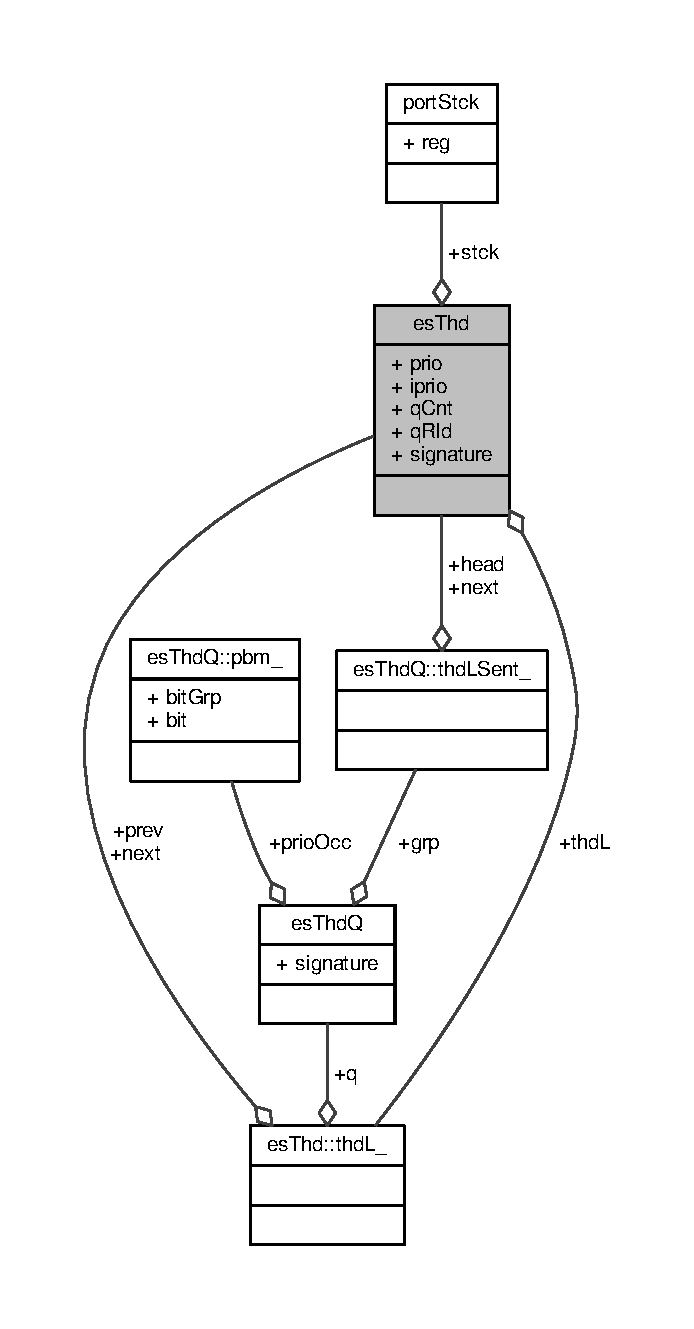
\includegraphics[height=550pt]{structesThd__coll__graph}
\end{center}
\end{figure}
\subsubsection*{Data Structures}
\begin{DoxyCompactItemize}
\item 
struct \hyperlink{structesThd_1_1thdL__}{thd\-L\-\_\-}
\begin{DoxyCompactList}\small\item\em Thread linked List structure. \end{DoxyCompactList}\end{DoxyCompactItemize}
\subsubsection*{Data Fields}
\begin{DoxyCompactItemize}
\item 
\hyperlink{group__template__cpu__intf_ga13cc91970e3e05fe4210440c068d3f4a}{port\-Stck\-\_\-\-T} $\ast$ \hyperlink{structesThd_a5a7906c650bc81f3f0639f6f8565316b}{stck}
\begin{DoxyCompactList}\small\item\em Pointer to thread's Top Of Stack. \end{DoxyCompactList}\item 
struct \hyperlink{structesThd_1_1thdL__}{es\-Thd\-::thd\-L\-\_\-} \hyperlink{structesThd_a69f72ac3b1f6199da48b41804f353325}{thd\-L}
\begin{DoxyCompactList}\small\item\em Thread linked list. \end{DoxyCompactList}\item 
uint\-\_\-fast8\-\_\-t \hyperlink{structesThd_a8d1877cabc7d4e637f96f4b4d5b0da09}{prio}
\begin{DoxyCompactList}\small\item\em Thread priority level. \end{DoxyCompactList}\item 
uint\-\_\-fast8\-\_\-t \hyperlink{structesThd_ad21505b1a302ea26fd073f7f67da3e84}{iprio}
\begin{DoxyCompactList}\small\item\em Initial Thread Priority level. \end{DoxyCompactList}\item 
uint\-\_\-fast8\-\_\-t \hyperlink{structesThd_a5721e76b02321c6701e52a9788d9bf1e}{q\-Cnt}
\begin{DoxyCompactList}\small\item\em Quantum counter. \end{DoxyCompactList}\item 
uint\-\_\-fast8\-\_\-t \hyperlink{structesThd_a3c2c5e4b699e3c990e37000650f031ba}{q\-Rld}
\begin{DoxyCompactList}\small\item\em Quantum counter reload value. \end{DoxyCompactList}\item 
port\-Reg\-\_\-\-T \hyperlink{structesThd_a72e6c4660e827aae5a621894756a5eb2}{signature}
\begin{DoxyCompactList}\small\item\em Thread structure signature. \end{DoxyCompactList}\end{DoxyCompactItemize}


\subsubsection{Detailed Description}
Thread structure. 

A thread structure is a data structure used by kernel to maintain information about a thread. Each thread requires its own I\-D structure and the structure is allocated in user memory space (R\-A\-M). The address of the thread’s I\-D structure is provided to O\-S thread-\/related services.

Thread structure is used as thread I\-D and a thread is always referenced using this structure. \begin{DoxyParagraph}{Object class\-:}
Regular {\bfseries A\-P\-I} object, this object is part of the application programming interface. 
\end{DoxyParagraph}


\subsubsection{Field Documentation}
\hypertarget{structesThd_a5a7906c650bc81f3f0639f6f8565316b}{\index{es\-Thd@{es\-Thd}!stck@{stck}}
\index{stck@{stck}!esThd@{es\-Thd}}
\paragraph[{stck}]{\setlength{\rightskip}{0pt plus 5cm}{\bf port\-Stck\-\_\-\-T}$\ast$ es\-Thd\-::stck}}\label{structesThd_a5a7906c650bc81f3f0639f6f8565316b}


Pointer to thread's Top Of Stack. 

\hypertarget{structesThd_a69f72ac3b1f6199da48b41804f353325}{\index{es\-Thd@{es\-Thd}!thd\-L@{thd\-L}}
\index{thd\-L@{thd\-L}!esThd@{es\-Thd}}
\paragraph[{thd\-L}]{\setlength{\rightskip}{0pt plus 5cm}struct {\bf es\-Thd\-::thd\-L\-\_\-}                es\-Thd\-::thd\-L}}\label{structesThd_a69f72ac3b1f6199da48b41804f353325}


Thread linked list. 

\hypertarget{structesThd_a8d1877cabc7d4e637f96f4b4d5b0da09}{\index{es\-Thd@{es\-Thd}!prio@{prio}}
\index{prio@{prio}!esThd@{es\-Thd}}
\paragraph[{prio}]{\setlength{\rightskip}{0pt plus 5cm}uint\-\_\-fast8\-\_\-t es\-Thd\-::prio}}\label{structesThd_a8d1877cabc7d4e637f96f4b4d5b0da09}


Thread priority level. 

\hypertarget{structesThd_ad21505b1a302ea26fd073f7f67da3e84}{\index{es\-Thd@{es\-Thd}!iprio@{iprio}}
\index{iprio@{iprio}!esThd@{es\-Thd}}
\paragraph[{iprio}]{\setlength{\rightskip}{0pt plus 5cm}uint\-\_\-fast8\-\_\-t es\-Thd\-::iprio}}\label{structesThd_ad21505b1a302ea26fd073f7f67da3e84}


Initial Thread Priority level. 

\hypertarget{structesThd_a5721e76b02321c6701e52a9788d9bf1e}{\index{es\-Thd@{es\-Thd}!q\-Cnt@{q\-Cnt}}
\index{q\-Cnt@{q\-Cnt}!esThd@{es\-Thd}}
\paragraph[{q\-Cnt}]{\setlength{\rightskip}{0pt plus 5cm}uint\-\_\-fast8\-\_\-t es\-Thd\-::q\-Cnt}}\label{structesThd_a5721e76b02321c6701e52a9788d9bf1e}


Quantum counter. 

\hypertarget{structesThd_a3c2c5e4b699e3c990e37000650f031ba}{\index{es\-Thd@{es\-Thd}!q\-Rld@{q\-Rld}}
\index{q\-Rld@{q\-Rld}!esThd@{es\-Thd}}
\paragraph[{q\-Rld}]{\setlength{\rightskip}{0pt plus 5cm}uint\-\_\-fast8\-\_\-t es\-Thd\-::q\-Rld}}\label{structesThd_a3c2c5e4b699e3c990e37000650f031ba}


Quantum counter reload value. 

\hypertarget{structesThd_a72e6c4660e827aae5a621894756a5eb2}{\index{es\-Thd@{es\-Thd}!signature@{signature}}
\index{signature@{signature}!esThd@{es\-Thd}}
\paragraph[{signature}]{\setlength{\rightskip}{0pt plus 5cm}port\-Reg\-\_\-\-T es\-Thd\-::signature}}\label{structesThd_a72e6c4660e827aae5a621894756a5eb2}


Thread structure signature. 



The documentation for this struct was generated from the following file\-:\begin{DoxyCompactItemize}
\item 
\hyperlink{kernel_8h}{kernel.\-h}\end{DoxyCompactItemize}

\hypertarget{structesThdQ}{\subsection{es\-Thd\-Q Struct Reference}
\label{structesThdQ}\index{es\-Thd\-Q@{es\-Thd\-Q}}
}


Thread Queue structure.  




{\ttfamily \#include $<$kernel.\-h$>$}



Collaboration diagram for es\-Thd\-Q\-:\nopagebreak
\begin{figure}[H]
\begin{center}
\leavevmode
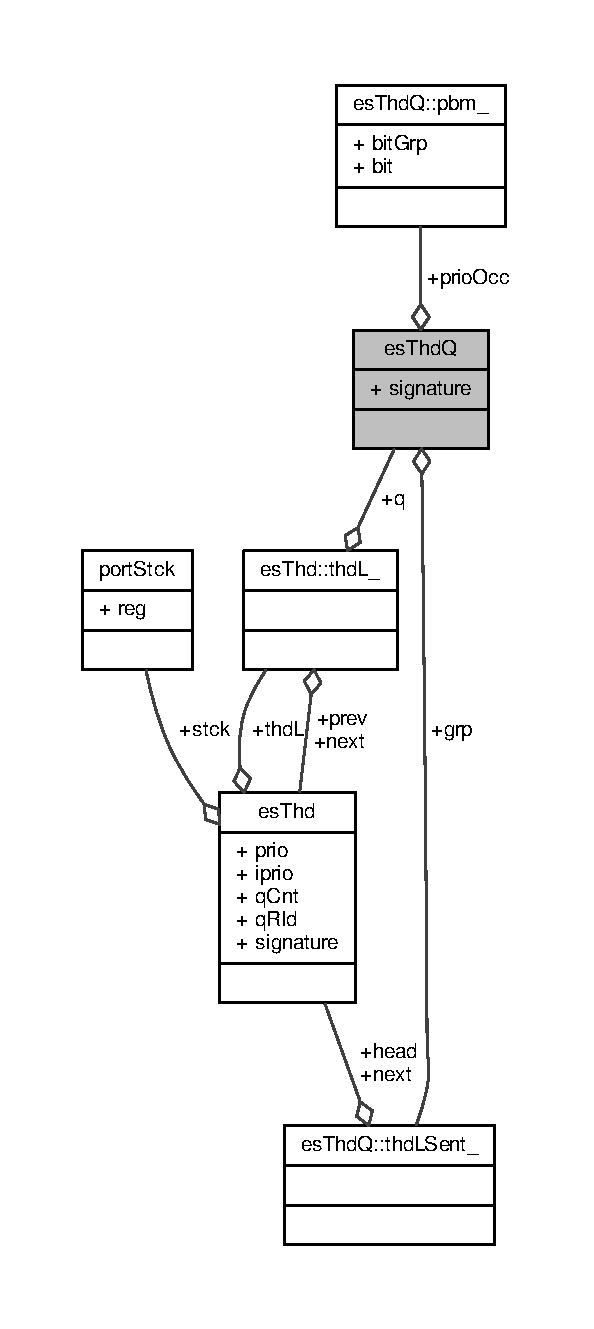
\includegraphics[height=550pt]{structesThdQ__coll__graph}
\end{center}
\end{figure}
\subsubsection*{Data Structures}
\begin{DoxyCompactItemize}
\item 
struct \hyperlink{structesThdQ_1_1pbm__}{pbm\-\_\-}
\begin{DoxyCompactList}\small\item\em Priority Bit Map structure. \end{DoxyCompactList}\item 
struct \hyperlink{structesThdQ_1_1thdLSent__}{thd\-L\-Sent\-\_\-}
\begin{DoxyCompactList}\small\item\em Thread linked list sentinel structure. \end{DoxyCompactList}\end{DoxyCompactItemize}
\subsubsection*{Data Fields}
\begin{DoxyCompactItemize}
\item 
struct \hyperlink{structesThdQ_1_1pbm__}{es\-Thd\-Q\-::pbm\-\_\-} \hyperlink{structesThdQ_a3ded234a55356bb708c55339d8438b0a}{prio\-Occ}
\begin{DoxyCompactList}\small\item\em Priority Occupancy. \end{DoxyCompactList}\item 
struct \hyperlink{structesThdQ_1_1thdLSent__}{es\-Thd\-Q\-::thd\-L\-Sent\-\_\-} \hyperlink{structesThdQ_ac658d22a97cdceefa9d72c3e9e1a675e}{grp} \mbox{[}\hyperlink{group__template__kern__cfg_ga56bd89fe76f7fe22f3d8805bc3c68892}{C\-F\-G\-\_\-\-S\-C\-H\-E\-D\-\_\-\-P\-R\-I\-O\-\_\-\-L\-V\-L}\mbox{]}
\begin{DoxyCompactList}\small\item\em Array of thread linked list sentinel structures. \end{DoxyCompactList}\item 
port\-Reg\-\_\-\-T \hyperlink{structesThdQ_a2756407c94319267cbf5d30814182b4d}{signature}
\begin{DoxyCompactList}\small\item\em Thread Queue struct signature. \end{DoxyCompactList}\end{DoxyCompactItemize}


\subsubsection{Detailed Description}
Thread Queue structure. 

\begin{DoxyParagraph}{Object class\-:}
Regular {\bfseries A\-P\-I} object, this object is part of the application programming interface. 
\end{DoxyParagraph}


\subsubsection{Field Documentation}
\hypertarget{structesThdQ_a3ded234a55356bb708c55339d8438b0a}{\index{es\-Thd\-Q@{es\-Thd\-Q}!prio\-Occ@{prio\-Occ}}
\index{prio\-Occ@{prio\-Occ}!esThdQ@{es\-Thd\-Q}}
\paragraph[{prio\-Occ}]{\setlength{\rightskip}{0pt plus 5cm}struct {\bf es\-Thd\-Q\-::pbm\-\_\-}                es\-Thd\-Q\-::prio\-Occ}}\label{structesThdQ_a3ded234a55356bb708c55339d8438b0a}


Priority Occupancy. 

\hypertarget{structesThdQ_ac658d22a97cdceefa9d72c3e9e1a675e}{\index{es\-Thd\-Q@{es\-Thd\-Q}!grp@{grp}}
\index{grp@{grp}!esThdQ@{es\-Thd\-Q}}
\paragraph[{grp}]{\setlength{\rightskip}{0pt plus 5cm}struct {\bf es\-Thd\-Q\-::thd\-L\-Sent\-\_\-}                es\-Thd\-Q\-::grp\mbox{[}{\bf C\-F\-G\-\_\-\-S\-C\-H\-E\-D\-\_\-\-P\-R\-I\-O\-\_\-\-L\-V\-L}\mbox{]}}}\label{structesThdQ_ac658d22a97cdceefa9d72c3e9e1a675e}


Array of thread linked list sentinel structures. 

\hypertarget{structesThdQ_a2756407c94319267cbf5d30814182b4d}{\index{es\-Thd\-Q@{es\-Thd\-Q}!signature@{signature}}
\index{signature@{signature}!esThdQ@{es\-Thd\-Q}}
\paragraph[{signature}]{\setlength{\rightskip}{0pt plus 5cm}port\-Reg\-\_\-\-T es\-Thd\-Q\-::signature}}\label{structesThdQ_a2756407c94319267cbf5d30814182b4d}


Thread Queue struct signature. 



The documentation for this struct was generated from the following file\-:\begin{DoxyCompactItemize}
\item 
\hyperlink{kernel_8h}{kernel.\-h}\end{DoxyCompactItemize}

\hypertarget{structesVTmr}{\subsection{es\-V\-Tmr Struct Reference}
\label{structesVTmr}\index{es\-V\-Tmr@{es\-V\-Tmr}}
}


Virtual Timer structure.  




{\ttfamily \#include $<$kernel.\-h$>$}



Collaboration diagram for es\-V\-Tmr\-:\nopagebreak
\begin{figure}[H]
\begin{center}
\leavevmode
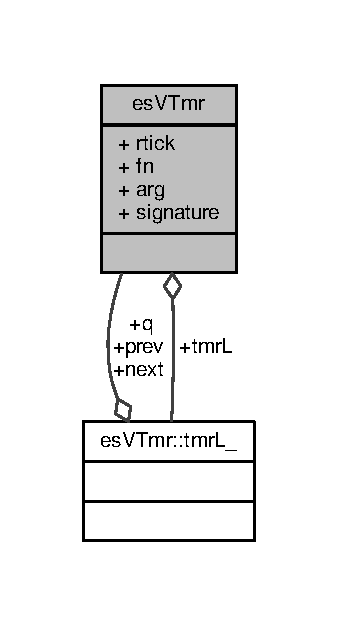
\includegraphics[width=156pt]{structesVTmr__coll__graph}
\end{center}
\end{figure}
\subsubsection*{Data Structures}
\begin{DoxyCompactItemize}
\item 
struct \hyperlink{structesVTmr_1_1tmrL}{tmr\-L}
\begin{DoxyCompactList}\small\item\em Virtual Timer linked list structure. \end{DoxyCompactList}\end{DoxyCompactItemize}
\subsubsection*{Data Fields}
\begin{DoxyCompactItemize}
\item 
struct \hyperlink{structesVTmr_1_1tmrL}{es\-V\-Tmr\-::tmr\-L} \hyperlink{structesVTmr_aa361779ab411157047bb0933acf2f9ab}{tmr\-L}
\begin{DoxyCompactList}\small\item\em Virtual Timer linked List. \end{DoxyCompactList}\item 
\hyperlink{group__kern__intf_ga844873888c186ee81eb66620dadb0451}{es\-Tick\-\_\-\-T} \hyperlink{structesVTmr_a4bbde49720b6aa0cc97e932ccb0383ea}{rtick}
\begin{DoxyCompactList}\small\item\em Relative tick value. \end{DoxyCompactList}\item 
void($\ast$ \hyperlink{structesVTmr_a17137ebfaf21de24d136b7d9b1390ddc}{fn} )(void $\ast$)
\begin{DoxyCompactList}\small\item\em Callback function pointer. \end{DoxyCompactList}\item 
void $\ast$ \hyperlink{structesVTmr_a4bd88651471b32f1fe71b4cec22756c0}{arg}
\begin{DoxyCompactList}\small\item\em Callback function argument. \end{DoxyCompactList}\item 
\hyperlink{group__template__cpu__intf_ga99980ab56ce9857e7380210d12e3d41f}{port\-Reg\-\_\-\-T} \hyperlink{structesVTmr_a8a620761f277b95ead5fc6f52c898daf}{signature}
\begin{DoxyCompactList}\small\item\em Timer structure signature, see \hyperlink{errors}{Debug\-: Error checking}. \end{DoxyCompactList}\end{DoxyCompactItemize}


\subsubsection{Detailed Description}
Virtual Timer structure. 

\subsubsection{Field Documentation}
\hypertarget{structesVTmr_aa361779ab411157047bb0933acf2f9ab}{\index{es\-V\-Tmr@{es\-V\-Tmr}!tmr\-L@{tmr\-L}}
\index{tmr\-L@{tmr\-L}!esVTmr@{es\-V\-Tmr}}
\paragraph[{tmr\-L}]{\setlength{\rightskip}{0pt plus 5cm}struct {\bf es\-V\-Tmr\-::tmr\-L}                {\bf es\-V\-Tmr\-::tmr\-L}}}\label{structesVTmr_aa361779ab411157047bb0933acf2f9ab}


Virtual Timer linked List. 

\hypertarget{structesVTmr_a4bbde49720b6aa0cc97e932ccb0383ea}{\index{es\-V\-Tmr@{es\-V\-Tmr}!rtick@{rtick}}
\index{rtick@{rtick}!esVTmr@{es\-V\-Tmr}}
\paragraph[{rtick}]{\setlength{\rightskip}{0pt plus 5cm}{\bf es\-Tick\-\_\-\-T} es\-V\-Tmr\-::rtick}}\label{structesVTmr_a4bbde49720b6aa0cc97e932ccb0383ea}


Relative tick value. 

\hypertarget{structesVTmr_a17137ebfaf21de24d136b7d9b1390ddc}{\index{es\-V\-Tmr@{es\-V\-Tmr}!fn@{fn}}
\index{fn@{fn}!esVTmr@{es\-V\-Tmr}}
\paragraph[{fn}]{\setlength{\rightskip}{0pt plus 5cm}void($\ast$  es\-V\-Tmr\-::fn)(void $\ast$)}}\label{structesVTmr_a17137ebfaf21de24d136b7d9b1390ddc}


Callback function pointer. 

\hypertarget{structesVTmr_a4bd88651471b32f1fe71b4cec22756c0}{\index{es\-V\-Tmr@{es\-V\-Tmr}!arg@{arg}}
\index{arg@{arg}!esVTmr@{es\-V\-Tmr}}
\paragraph[{arg}]{\setlength{\rightskip}{0pt plus 5cm}void$\ast$ es\-V\-Tmr\-::arg}}\label{structesVTmr_a4bd88651471b32f1fe71b4cec22756c0}


Callback function argument. 

\hypertarget{structesVTmr_a8a620761f277b95ead5fc6f52c898daf}{\index{es\-V\-Tmr@{es\-V\-Tmr}!signature@{signature}}
\index{signature@{signature}!esVTmr@{es\-V\-Tmr}}
\paragraph[{signature}]{\setlength{\rightskip}{0pt plus 5cm}{\bf port\-Reg\-\_\-\-T} es\-V\-Tmr\-::signature}}\label{structesVTmr_a8a620761f277b95ead5fc6f52c898daf}


Timer structure signature, see \hyperlink{errors}{Debug\-: Error checking}. 



The documentation for this struct was generated from the following file\-:\begin{DoxyCompactItemize}
\item 
\hyperlink{kernel_8h}{kernel.\-h}\end{DoxyCompactItemize}

\hypertarget{structkernCtrl__}{\subsection{kern\-Ctrl\-\_\- Struct Reference}
\label{structkernCtrl__}\index{kern\-Ctrl\-\_\-@{kern\-Ctrl\-\_\-}}
}


Kernel control block structure.  




{\ttfamily \#include $<$kernel.\-h$>$}



Collaboration diagram for kern\-Ctrl\-\_\-\-:\nopagebreak
\begin{figure}[H]
\begin{center}
\leavevmode
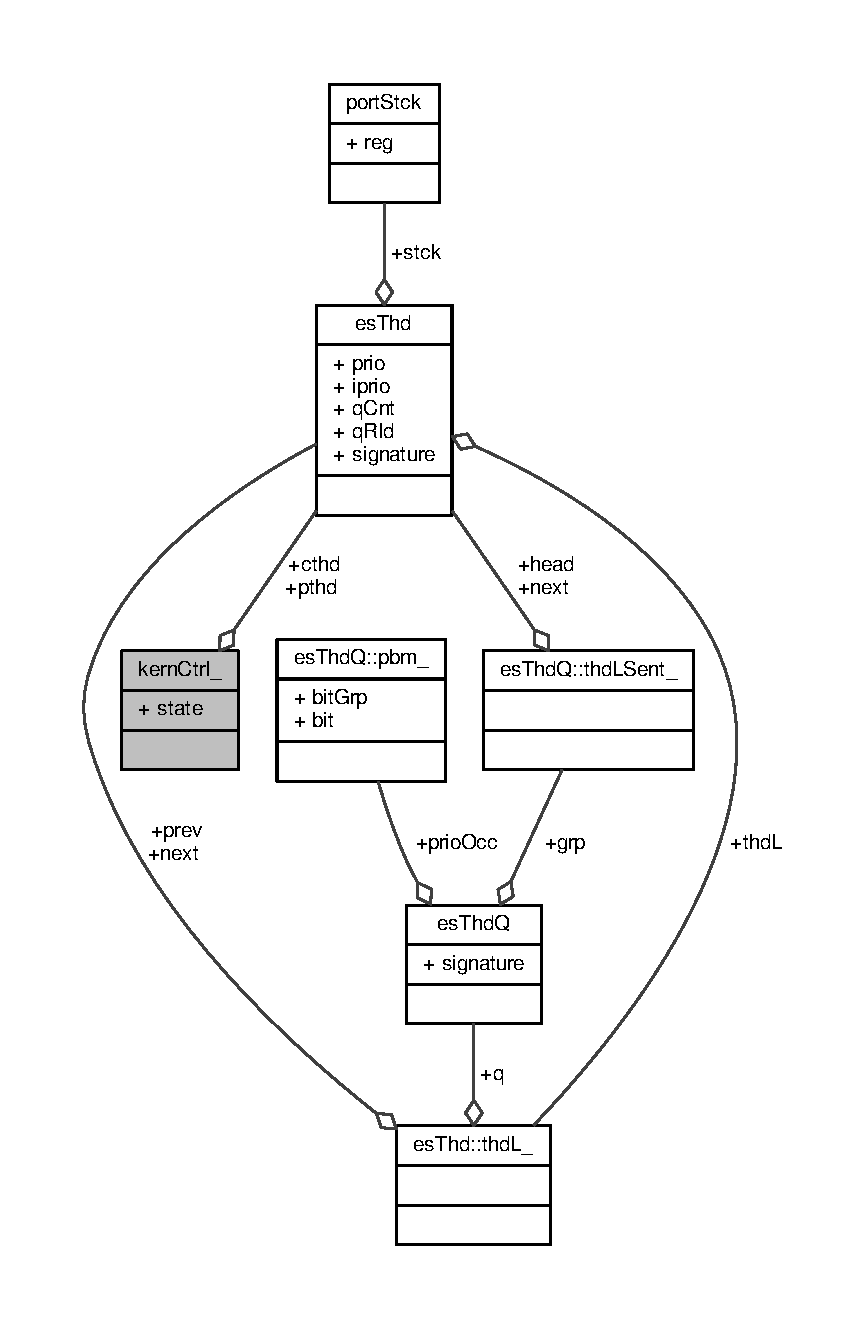
\includegraphics[width=350pt]{structkernCtrl____coll__graph}
\end{center}
\end{figure}
\subsubsection*{Data Fields}
\begin{DoxyCompactItemize}
\item 
struct \hyperlink{structesThd}{es\-Thd} $\ast$ \hyperlink{structkernCtrl___ada8492a441474dd8243f9b3d6440b931}{cthd}
\begin{DoxyCompactList}\small\item\em Pointer to the Current Thread. \end{DoxyCompactList}\item 
struct \hyperlink{structesThd}{es\-Thd} $\ast$ \hyperlink{structkernCtrl___aba053a184d6eedce8df1788a0ca5955e}{pthd}
\begin{DoxyCompactList}\small\item\em Pointer to the Pending Thread to be switched. \end{DoxyCompactList}\item 
enum \hyperlink{group__kern__ctrl_gac9be6bfeddbd6af148cdb3867fbc24af}{es\-Kern\-State} \hyperlink{structkernCtrl___af9186609ce09f0a53278e95ccd5c36ec}{state}
\begin{DoxyCompactList}\small\item\em State of kernel. \end{DoxyCompactList}\end{DoxyCompactItemize}


\subsubsection{Detailed Description}
Kernel control block structure. 

This structure holds important status data about the kernel. Since all data within the structure is somewhat related and accessed within the same pieces of code it was decided it is better to group all kernel data into the structure. This way the compiler can generate code that gets the address of the structure and then use relative indirect addressing to access all members of the structure. This results in more efficient code on architectures that have relative indirect addressing capability. \begin{DoxyParagraph}{Object class\-:}
{\bfseries Not A\-P\-I} object, this object is not part of the application programming interface and it is intended for internal use only. 
\end{DoxyParagraph}


\subsubsection{Field Documentation}
\hypertarget{structkernCtrl___ada8492a441474dd8243f9b3d6440b931}{\index{kern\-Ctrl\-\_\-@{kern\-Ctrl\-\_\-}!cthd@{cthd}}
\index{cthd@{cthd}!kernCtrl_@{kern\-Ctrl\-\_\-}}
\paragraph[{cthd}]{\setlength{\rightskip}{0pt plus 5cm}struct {\bf es\-Thd}$\ast$ kern\-Ctrl\-\_\-\-::cthd}}\label{structkernCtrl___ada8492a441474dd8243f9b3d6440b931}


Pointer to the Current Thread. 

\hypertarget{structkernCtrl___aba053a184d6eedce8df1788a0ca5955e}{\index{kern\-Ctrl\-\_\-@{kern\-Ctrl\-\_\-}!pthd@{pthd}}
\index{pthd@{pthd}!kernCtrl_@{kern\-Ctrl\-\_\-}}
\paragraph[{pthd}]{\setlength{\rightskip}{0pt plus 5cm}struct {\bf es\-Thd}$\ast$ kern\-Ctrl\-\_\-\-::pthd}}\label{structkernCtrl___aba053a184d6eedce8df1788a0ca5955e}


Pointer to the Pending Thread to be switched. 

\hypertarget{structkernCtrl___af9186609ce09f0a53278e95ccd5c36ec}{\index{kern\-Ctrl\-\_\-@{kern\-Ctrl\-\_\-}!state@{state}}
\index{state@{state}!kernCtrl_@{kern\-Ctrl\-\_\-}}
\paragraph[{state}]{\setlength{\rightskip}{0pt plus 5cm}enum {\bf es\-Kern\-State} kern\-Ctrl\-\_\-\-::state}}\label{structkernCtrl___af9186609ce09f0a53278e95ccd5c36ec}


State of kernel. 



The documentation for this struct was generated from the following file\-:\begin{DoxyCompactItemize}
\item 
\hyperlink{kernel_8h}{kernel.\-h}\end{DoxyCompactItemize}

\hypertarget{structesThdQ_1_1pbm__}{\subsection{es\-Thd\-Q\-:\-:pbm\-\_\- Struct Reference}
\label{structesThdQ_1_1pbm__}\index{es\-Thd\-Q\-::pbm\-\_\-@{es\-Thd\-Q\-::pbm\-\_\-}}
}


Priority Bit Map structure.  




{\ttfamily \#include $<$kernel.\-h$>$}



Collaboration diagram for es\-Thd\-Q\-:\-:pbm\-\_\-\-:\nopagebreak
\begin{figure}[H]
\begin{center}
\leavevmode
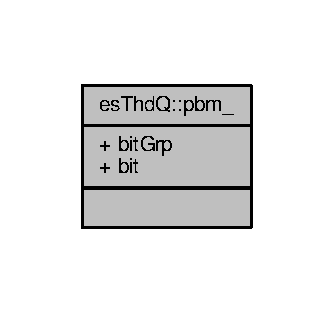
\includegraphics[width=160pt]{structesThdQ_1_1pbm____coll__graph}
\end{center}
\end{figure}
\subsubsection*{Data Fields}
\begin{DoxyCompactItemize}
\item 
port\-Reg\-\_\-\-T \hyperlink{structesThdQ_1_1pbm___aa24f418263c2f73a4a38d7f01fa3460a}{bit\-Grp}
\begin{DoxyCompactList}\small\item\em Bit group indicator. \end{DoxyCompactList}\item 
port\-Reg\-\_\-\-T \hyperlink{structesThdQ_1_1pbm___a3ba3044daa9e71d5e38acd0277dc9c58}{bit} \mbox{[}E\-S\-\_\-\-D\-I\-V\-\_\-\-R\-O\-U\-N\-D\-U\-P(\hyperlink{group__template__kern__cfg_ga56bd89fe76f7fe22f3d8805bc3c68892}{C\-F\-G\-\_\-\-S\-C\-H\-E\-D\-\_\-\-P\-R\-I\-O\-\_\-\-L\-V\-L}, P\-O\-R\-T\-\_\-\-D\-E\-F\-\_\-\-D\-A\-T\-A\-\_\-\-W\-I\-D\-T\-H)\mbox{]}
\begin{DoxyCompactList}\small\item\em Bit priority indicator. \end{DoxyCompactList}\end{DoxyCompactItemize}


\subsubsection{Detailed Description}
Priority Bit Map structure. 

\begin{DoxyParagraph}{Object class\-:}
{\bfseries Not A\-P\-I} object, this object is not part of the application programming interface and it is intended for internal use only. 
\end{DoxyParagraph}


\subsubsection{Field Documentation}
\hypertarget{structesThdQ_1_1pbm___aa24f418263c2f73a4a38d7f01fa3460a}{\index{es\-Thd\-Q\-::pbm\-\_\-@{es\-Thd\-Q\-::pbm\-\_\-}!bit\-Grp@{bit\-Grp}}
\index{bit\-Grp@{bit\-Grp}!esThdQ::pbm_@{es\-Thd\-Q\-::pbm\-\_\-}}
\paragraph[{bit\-Grp}]{\setlength{\rightskip}{0pt plus 5cm}port\-Reg\-\_\-\-T es\-Thd\-Q\-::pbm\-\_\-\-::bit\-Grp}}\label{structesThdQ_1_1pbm___aa24f418263c2f73a4a38d7f01fa3460a}


Bit group indicator. 

\hypertarget{structesThdQ_1_1pbm___a3ba3044daa9e71d5e38acd0277dc9c58}{\index{es\-Thd\-Q\-::pbm\-\_\-@{es\-Thd\-Q\-::pbm\-\_\-}!bit@{bit}}
\index{bit@{bit}!esThdQ::pbm_@{es\-Thd\-Q\-::pbm\-\_\-}}
\paragraph[{bit}]{\setlength{\rightskip}{0pt plus 5cm}port\-Reg\-\_\-\-T es\-Thd\-Q\-::pbm\-\_\-\-::bit\mbox{[}E\-S\-\_\-\-D\-I\-V\-\_\-\-R\-O\-U\-N\-D\-U\-P({\bf C\-F\-G\-\_\-\-S\-C\-H\-E\-D\-\_\-\-P\-R\-I\-O\-\_\-\-L\-V\-L}, P\-O\-R\-T\-\_\-\-D\-E\-F\-\_\-\-D\-A\-T\-A\-\_\-\-W\-I\-D\-T\-H)\mbox{]}}}\label{structesThdQ_1_1pbm___a3ba3044daa9e71d5e38acd0277dc9c58}


Bit priority indicator. 



The documentation for this struct was generated from the following file\-:\begin{DoxyCompactItemize}
\item 
\hyperlink{kernel_8h}{kernel.\-h}\end{DoxyCompactItemize}

\hypertarget{structportCtx}{\subsection{port\-Ctx Struct Reference}
\label{structportCtx}\index{port\-Ctx@{port\-Ctx}}
}


Port context structure.  




{\ttfamily \#include $<$kcore.\-h$>$}



Collaboration diagram for port\-Ctx\-:\nopagebreak
\begin{figure}[H]
\begin{center}
\leavevmode
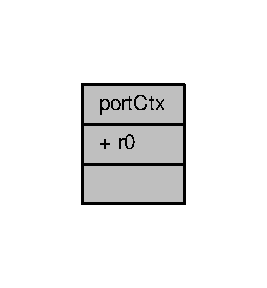
\includegraphics[width=128pt]{structportCtx__coll__graph}
\end{center}
\end{figure}
\subsubsection*{Data Fields}
\begin{DoxyCompactItemize}
\item 
port\-Reg\-\_\-\-T \hyperlink{structportCtx_a0ee17f42c9b473ddb96365e05c71f086}{r0}
\begin{DoxyCompactList}\small\item\em Data pushed on stack during context switching. \end{DoxyCompactList}\end{DoxyCompactItemize}


\subsubsection{Detailed Description}
Port context structure. 

\subsubsection{Field Documentation}
\hypertarget{structportCtx_a0ee17f42c9b473ddb96365e05c71f086}{\index{port\-Ctx@{port\-Ctx}!r0@{r0}}
\index{r0@{r0}!portCtx@{port\-Ctx}}
\paragraph[{r0}]{\setlength{\rightskip}{0pt plus 5cm}port\-Reg\-\_\-\-T port\-Ctx\-::r0}}\label{structportCtx_a0ee17f42c9b473ddb96365e05c71f086}


Data pushed on stack during context switching. 



The documentation for this struct was generated from the following file\-:\begin{DoxyCompactItemize}
\item 
\hyperlink{kcore_8h}{kcore.\-h}\end{DoxyCompactItemize}

\hypertarget{structportStck}{\subsection{port\-Stck Struct Reference}
\label{structportStck}\index{port\-Stck@{port\-Stck}}
}


Stack structure used for stack declaration in order to force the alignment Alignment of stack structure.  




{\ttfamily \#include $<$cpu.\-h$>$}



Collaboration diagram for port\-Stck\-:\nopagebreak
\begin{figure}[H]
\begin{center}
\leavevmode
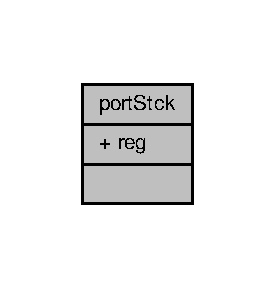
\includegraphics[width=132pt]{structportStck__coll__graph}
\end{center}
\end{figure}
\subsubsection*{Data Fields}
\begin{DoxyCompactItemize}
\item 
\hyperlink{group__template__cpu__intf_ga99980ab56ce9857e7380210d12e3d41f}{port\-Reg\-\_\-\-T} \hyperlink{structportStck_a52e715773895c635b3e8ddb30d582d9c}{reg}
\begin{DoxyCompactList}\small\item\em A structure field representing stack data. \end{DoxyCompactList}\end{DoxyCompactItemize}


\subsubsection{Detailed Description}
Stack structure used for stack declaration in order to force the alignment Alignment of stack structure. 

\subsubsection{Field Documentation}
\hypertarget{structportStck_a52e715773895c635b3e8ddb30d582d9c}{\index{port\-Stck@{port\-Stck}!reg@{reg}}
\index{reg@{reg}!portStck@{port\-Stck}}
\paragraph[{reg}]{\setlength{\rightskip}{0pt plus 5cm}{\bf port\-Reg\-\_\-\-T} port\-Stck\-::reg}}\label{structportStck_a52e715773895c635b3e8ddb30d582d9c}


A structure field representing stack data. 



The documentation for this struct was generated from the following file\-:\begin{DoxyCompactItemize}
\item 
\hyperlink{cpu_8h}{cpu.\-h}\end{DoxyCompactItemize}

\hypertarget{structsysTmr}{\subsection{sys\-Tmr Struct Reference}
\label{structsysTmr}\index{sys\-Tmr@{sys\-Tmr}}
}


Main System Timer structure.  




Collaboration diagram for sys\-Tmr\-:\nopagebreak
\begin{figure}[H]
\begin{center}
\leavevmode
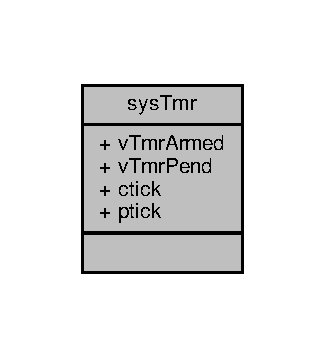
\includegraphics[width=156pt]{structsysTmr__coll__graph}
\end{center}
\end{figure}
\subsubsection*{Data Fields}
\begin{DoxyCompactItemize}
\item 
uint\-\_\-fast16\-\_\-t \hyperlink{structsysTmr_a3fb347fcb0b2bda6795f5dd8c4413873}{v\-Tmr\-Armed}
\begin{DoxyCompactList}\small\item\em The number of armed virtual timers in system. \end{DoxyCompactList}\item 
uint\-\_\-fast16\-\_\-t \hyperlink{structsysTmr_a63badc568f8fde1dd566e1f456aab008}{v\-Tmr\-Pend}
\begin{DoxyCompactList}\small\item\em The number of pending timers for arming. \end{DoxyCompactList}\item 
\hyperlink{group__kern__vtmr_ga844873888c186ee81eb66620dadb0451}{es\-Tick\-\_\-\-T} \hyperlink{structsysTmr_a1f1fac425438fad41278db9f2865d0a3}{ctick}
\begin{DoxyCompactList}\small\item\em Current system timer tick value. \end{DoxyCompactList}\item 
\hyperlink{group__kern__vtmr_ga844873888c186ee81eb66620dadb0451}{es\-Tick\-\_\-\-T} \hyperlink{structsysTmr_a338f10146bdac2bdd69447fca0fe75f8}{ptick}
\begin{DoxyCompactList}\small\item\em Pending ticks during the timer sleep mode. \end{DoxyCompactList}\end{DoxyCompactItemize}


\subsubsection{Detailed Description}
Main System Timer structure. 

\begin{DoxyNote}{Note}
1) Member {\ttfamily ptick} exists only if A\-D\-A\-P\-T\-I\-V\-E mode is selected. When this mode is selected then kernel supports more aggressive power savings. 
\end{DoxyNote}


\subsubsection{Field Documentation}
\hypertarget{structsysTmr_a3fb347fcb0b2bda6795f5dd8c4413873}{\index{sys\-Tmr@{sys\-Tmr}!v\-Tmr\-Armed@{v\-Tmr\-Armed}}
\index{v\-Tmr\-Armed@{v\-Tmr\-Armed}!sysTmr@{sys\-Tmr}}
\paragraph[{v\-Tmr\-Armed}]{\setlength{\rightskip}{0pt plus 5cm}uint\-\_\-fast16\-\_\-t sys\-Tmr\-::v\-Tmr\-Armed}}\label{structsysTmr_a3fb347fcb0b2bda6795f5dd8c4413873}


The number of armed virtual timers in system. 

\hypertarget{structsysTmr_a63badc568f8fde1dd566e1f456aab008}{\index{sys\-Tmr@{sys\-Tmr}!v\-Tmr\-Pend@{v\-Tmr\-Pend}}
\index{v\-Tmr\-Pend@{v\-Tmr\-Pend}!sysTmr@{sys\-Tmr}}
\paragraph[{v\-Tmr\-Pend}]{\setlength{\rightskip}{0pt plus 5cm}uint\-\_\-fast16\-\_\-t sys\-Tmr\-::v\-Tmr\-Pend}}\label{structsysTmr_a63badc568f8fde1dd566e1f456aab008}


The number of pending timers for arming. 

\hypertarget{structsysTmr_a1f1fac425438fad41278db9f2865d0a3}{\index{sys\-Tmr@{sys\-Tmr}!ctick@{ctick}}
\index{ctick@{ctick}!sysTmr@{sys\-Tmr}}
\paragraph[{ctick}]{\setlength{\rightskip}{0pt plus 5cm}{\bf es\-Tick\-\_\-\-T} sys\-Tmr\-::ctick}}\label{structsysTmr_a1f1fac425438fad41278db9f2865d0a3}


Current system timer tick value. 

\hypertarget{structsysTmr_a338f10146bdac2bdd69447fca0fe75f8}{\index{sys\-Tmr@{sys\-Tmr}!ptick@{ptick}}
\index{ptick@{ptick}!sysTmr@{sys\-Tmr}}
\paragraph[{ptick}]{\setlength{\rightskip}{0pt plus 5cm}{\bf es\-Tick\-\_\-\-T} sys\-Tmr\-::ptick}}\label{structsysTmr_a338f10146bdac2bdd69447fca0fe75f8}


Pending ticks during the timer sleep mode. 



The documentation for this struct was generated from the following file\-:\begin{DoxyCompactItemize}
\item 
\hyperlink{kernel_8c}{kernel.\-c}\end{DoxyCompactItemize}

\hypertarget{structesThd_1_1thdL__}{\subsection{es\-Thd\-:\-:thd\-L\-\_\- Struct Reference}
\label{structesThd_1_1thdL__}\index{es\-Thd\-::thd\-L\-\_\-@{es\-Thd\-::thd\-L\-\_\-}}
}


Thread linked List structure.  




{\ttfamily \#include $<$kernel.\-h$>$}



Collaboration diagram for es\-Thd\-:\-:thd\-L\-\_\-\-:\nopagebreak
\begin{figure}[H]
\begin{center}
\leavevmode
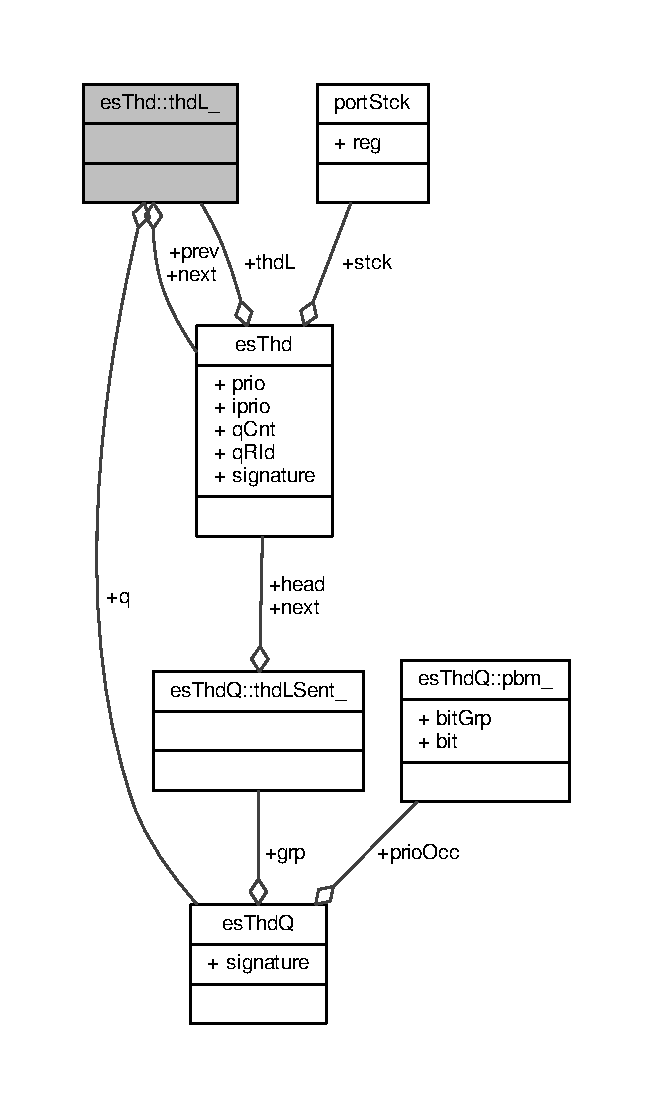
\includegraphics[width=313pt]{structesThd_1_1thdL____coll__graph}
\end{center}
\end{figure}
\subsubsection*{Data Fields}
\begin{DoxyCompactItemize}
\item 
struct \hyperlink{structesThdQ}{es\-Thd\-Q} $\ast$ \hyperlink{structesThd_1_1thdL___a4f8a154ac7c5423b1ff21521ba25fd0b}{q}
\begin{DoxyCompactList}\small\item\em Points to parent thread queue. \end{DoxyCompactList}\item 
struct \hyperlink{structesThd}{es\-Thd} $\ast$ \hyperlink{structesThd_1_1thdL___accf72efa113ca485b742791d680d92bb}{next}
\begin{DoxyCompactList}\small\item\em Next thread in linked list. \end{DoxyCompactList}\item 
struct \hyperlink{structesThd}{es\-Thd} $\ast$ \hyperlink{structesThd_1_1thdL___a1c3a34dae1d17063950b672684c5917e}{prev}
\begin{DoxyCompactList}\small\item\em Previous thread in linked list. \end{DoxyCompactList}\end{DoxyCompactItemize}


\subsubsection{Detailed Description}
Thread linked List structure. 

\begin{DoxyParagraph}{Object class\-:}
{\bfseries Not A\-P\-I} object, this object is not part of the application programming interface and it is intended for internal use only. 
\end{DoxyParagraph}


\subsubsection{Field Documentation}
\hypertarget{structesThd_1_1thdL___a4f8a154ac7c5423b1ff21521ba25fd0b}{\index{es\-Thd\-::thd\-L\-\_\-@{es\-Thd\-::thd\-L\-\_\-}!q@{q}}
\index{q@{q}!esThd::thdL_@{es\-Thd\-::thd\-L\-\_\-}}
\paragraph[{q}]{\setlength{\rightskip}{0pt plus 5cm}struct {\bf es\-Thd\-Q}$\ast$ es\-Thd\-::thd\-L\-\_\-\-::q}}\label{structesThd_1_1thdL___a4f8a154ac7c5423b1ff21521ba25fd0b}


Points to parent thread queue. 

\hypertarget{structesThd_1_1thdL___accf72efa113ca485b742791d680d92bb}{\index{es\-Thd\-::thd\-L\-\_\-@{es\-Thd\-::thd\-L\-\_\-}!next@{next}}
\index{next@{next}!esThd::thdL_@{es\-Thd\-::thd\-L\-\_\-}}
\paragraph[{next}]{\setlength{\rightskip}{0pt plus 5cm}struct {\bf es\-Thd}$\ast$ es\-Thd\-::thd\-L\-\_\-\-::next}}\label{structesThd_1_1thdL___accf72efa113ca485b742791d680d92bb}


Next thread in linked list. 

\hypertarget{structesThd_1_1thdL___a1c3a34dae1d17063950b672684c5917e}{\index{es\-Thd\-::thd\-L\-\_\-@{es\-Thd\-::thd\-L\-\_\-}!prev@{prev}}
\index{prev@{prev}!esThd::thdL_@{es\-Thd\-::thd\-L\-\_\-}}
\paragraph[{prev}]{\setlength{\rightskip}{0pt plus 5cm}struct {\bf es\-Thd}$\ast$ es\-Thd\-::thd\-L\-\_\-\-::prev}}\label{structesThd_1_1thdL___a1c3a34dae1d17063950b672684c5917e}


Previous thread in linked list. 



The documentation for this struct was generated from the following file\-:\begin{DoxyCompactItemize}
\item 
\hyperlink{kernel_8h}{kernel.\-h}\end{DoxyCompactItemize}

\hypertarget{structesThdQ_1_1thdLSent__}{\subsection{es\-Thd\-Q\-:\-:thd\-L\-Sent\-\_\- Struct Reference}
\label{structesThdQ_1_1thdLSent__}\index{es\-Thd\-Q\-::thd\-L\-Sent\-\_\-@{es\-Thd\-Q\-::thd\-L\-Sent\-\_\-}}
}


Thread linked list sentinel structure.  




{\ttfamily \#include $<$kernel.\-h$>$}



Collaboration diagram for es\-Thd\-Q\-:\-:thd\-L\-Sent\-\_\-\-:\nopagebreak
\begin{figure}[H]
\begin{center}
\leavevmode
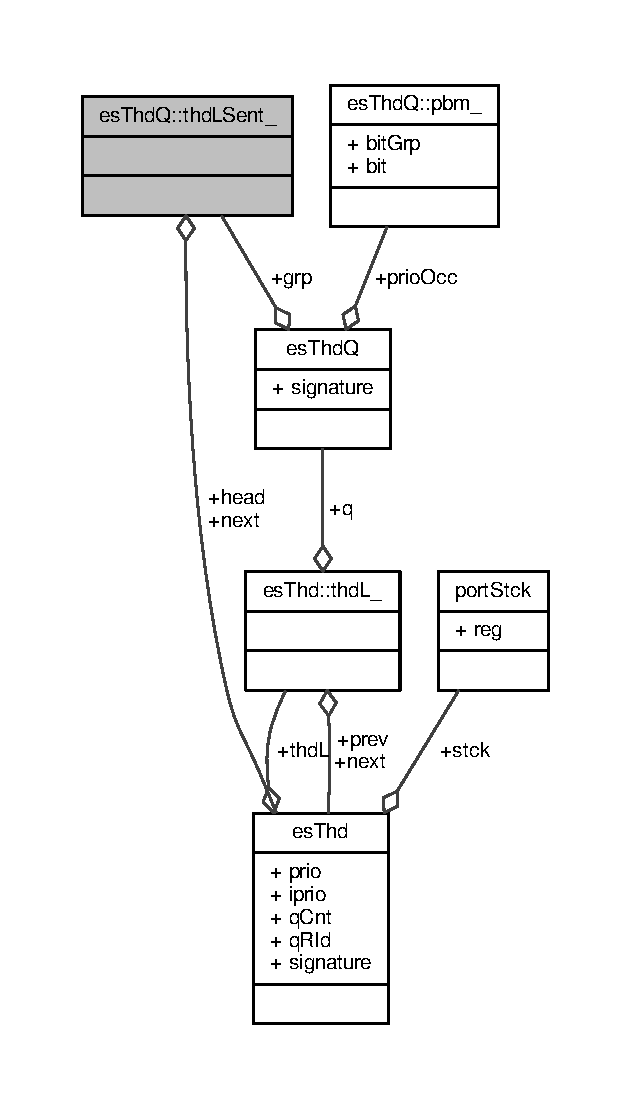
\includegraphics[width=303pt]{structesThdQ_1_1thdLSent____coll__graph}
\end{center}
\end{figure}
\subsubsection*{Data Fields}
\begin{DoxyCompactItemize}
\item 
struct \hyperlink{structesThd}{es\-Thd} $\ast$ \hyperlink{structesThdQ_1_1thdLSent___a88776574b11b8c0b27f97f9ef9a48a46}{head}
\begin{DoxyCompactList}\small\item\em Points to the first thread in linked list. \end{DoxyCompactList}\item 
struct \hyperlink{structesThd}{es\-Thd} $\ast$ \hyperlink{structesThdQ_1_1thdLSent___a0597468d0cfc6ac195d330d8ec7dde13}{next}
\begin{DoxyCompactList}\small\item\em Points to the next thread in linked list. \end{DoxyCompactList}\end{DoxyCompactItemize}


\subsubsection{Detailed Description}
Thread linked list sentinel structure. 

\begin{DoxyParagraph}{Object class\-:}
{\bfseries Not A\-P\-I} object, this object is not part of the application programming interface and it is intended for internal use only. 
\end{DoxyParagraph}


\subsubsection{Field Documentation}
\hypertarget{structesThdQ_1_1thdLSent___a88776574b11b8c0b27f97f9ef9a48a46}{\index{es\-Thd\-Q\-::thd\-L\-Sent\-\_\-@{es\-Thd\-Q\-::thd\-L\-Sent\-\_\-}!head@{head}}
\index{head@{head}!esThdQ::thdLSent_@{es\-Thd\-Q\-::thd\-L\-Sent\-\_\-}}
\paragraph[{head}]{\setlength{\rightskip}{0pt plus 5cm}struct {\bf es\-Thd}$\ast$ es\-Thd\-Q\-::thd\-L\-Sent\-\_\-\-::head}}\label{structesThdQ_1_1thdLSent___a88776574b11b8c0b27f97f9ef9a48a46}


Points to the first thread in linked list. 

\hypertarget{structesThdQ_1_1thdLSent___a0597468d0cfc6ac195d330d8ec7dde13}{\index{es\-Thd\-Q\-::thd\-L\-Sent\-\_\-@{es\-Thd\-Q\-::thd\-L\-Sent\-\_\-}!next@{next}}
\index{next@{next}!esThdQ::thdLSent_@{es\-Thd\-Q\-::thd\-L\-Sent\-\_\-}}
\paragraph[{next}]{\setlength{\rightskip}{0pt plus 5cm}struct {\bf es\-Thd}$\ast$ es\-Thd\-Q\-::thd\-L\-Sent\-\_\-\-::next}}\label{structesThdQ_1_1thdLSent___a0597468d0cfc6ac195d330d8ec7dde13}


Points to the next thread in linked list. 



The documentation for this struct was generated from the following file\-:\begin{DoxyCompactItemize}
\item 
\hyperlink{kernel_8h}{kernel.\-h}\end{DoxyCompactItemize}

\hypertarget{structesVTmr_1_1tmrL__}{\subsection{es\-V\-Tmr\-:\-:tmr\-L\-\_\- Struct Reference}
\label{structesVTmr_1_1tmrL__}\index{es\-V\-Tmr\-::tmr\-L\-\_\-@{es\-V\-Tmr\-::tmr\-L\-\_\-}}
}


Virtual Timer linked list structure.  




{\ttfamily \#include $<$kernel.\-h$>$}



Collaboration diagram for es\-V\-Tmr\-:\-:tmr\-L\-\_\-\-:\nopagebreak
\begin{figure}[H]
\begin{center}
\leavevmode
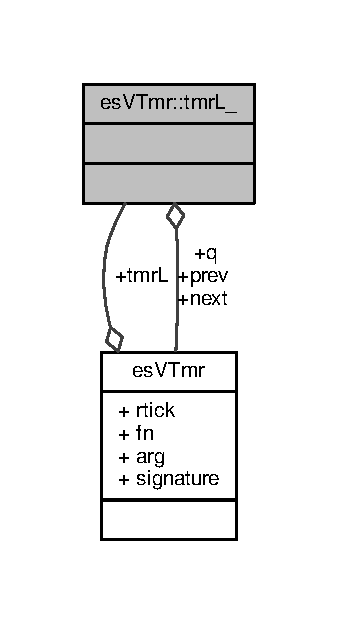
\includegraphics[width=162pt]{structesVTmr_1_1tmrL____coll__graph}
\end{center}
\end{figure}
\subsubsection*{Data Fields}
\begin{DoxyCompactItemize}
\item 
struct \hyperlink{structesVTmr}{es\-V\-Tmr} $\ast$ \hyperlink{structesVTmr_1_1tmrL___ac94cbec591cfa91217281a5a5eb58a18}{q}
\begin{DoxyCompactList}\small\item\em Points to parent timer queue. \end{DoxyCompactList}\item 
struct \hyperlink{structesVTmr}{es\-V\-Tmr} $\ast$ \hyperlink{structesVTmr_1_1tmrL___aecec9d50fcf431357a3d03428a56f97c}{next}
\begin{DoxyCompactList}\small\item\em Next thread in Virtual Timer linked list. \end{DoxyCompactList}\item 
struct \hyperlink{structesVTmr}{es\-V\-Tmr} $\ast$ \hyperlink{structesVTmr_1_1tmrL___af796db79ea86f16a9c976f0546e0dee5}{prev}
\begin{DoxyCompactList}\small\item\em Previous thread in virtual timer linked list. \end{DoxyCompactList}\end{DoxyCompactItemize}


\subsubsection{Detailed Description}
Virtual Timer linked list structure. 

\begin{DoxyParagraph}{Object class\-:}
{\bfseries Not A\-P\-I} object, this object is not part of the application programming interface and it is intended for internal use only. 
\end{DoxyParagraph}


\subsubsection{Field Documentation}
\hypertarget{structesVTmr_1_1tmrL___ac94cbec591cfa91217281a5a5eb58a18}{\index{es\-V\-Tmr\-::tmr\-L\-\_\-@{es\-V\-Tmr\-::tmr\-L\-\_\-}!q@{q}}
\index{q@{q}!esVTmr::tmrL_@{es\-V\-Tmr\-::tmr\-L\-\_\-}}
\paragraph[{q}]{\setlength{\rightskip}{0pt plus 5cm}struct {\bf es\-V\-Tmr}$\ast$ es\-V\-Tmr\-::tmr\-L\-\_\-\-::q}}\label{structesVTmr_1_1tmrL___ac94cbec591cfa91217281a5a5eb58a18}


Points to parent timer queue. 

\hypertarget{structesVTmr_1_1tmrL___aecec9d50fcf431357a3d03428a56f97c}{\index{es\-V\-Tmr\-::tmr\-L\-\_\-@{es\-V\-Tmr\-::tmr\-L\-\_\-}!next@{next}}
\index{next@{next}!esVTmr::tmrL_@{es\-V\-Tmr\-::tmr\-L\-\_\-}}
\paragraph[{next}]{\setlength{\rightskip}{0pt plus 5cm}struct {\bf es\-V\-Tmr}$\ast$ es\-V\-Tmr\-::tmr\-L\-\_\-\-::next}}\label{structesVTmr_1_1tmrL___aecec9d50fcf431357a3d03428a56f97c}


Next thread in Virtual Timer linked list. 

\hypertarget{structesVTmr_1_1tmrL___af796db79ea86f16a9c976f0546e0dee5}{\index{es\-V\-Tmr\-::tmr\-L\-\_\-@{es\-V\-Tmr\-::tmr\-L\-\_\-}!prev@{prev}}
\index{prev@{prev}!esVTmr::tmrL_@{es\-V\-Tmr\-::tmr\-L\-\_\-}}
\paragraph[{prev}]{\setlength{\rightskip}{0pt plus 5cm}struct {\bf es\-V\-Tmr}$\ast$ es\-V\-Tmr\-::tmr\-L\-\_\-\-::prev}}\label{structesVTmr_1_1tmrL___af796db79ea86f16a9c976f0546e0dee5}


Previous thread in virtual timer linked list. 



The documentation for this struct was generated from the following file\-:\begin{DoxyCompactItemize}
\item 
\hyperlink{kernel_8h}{kernel.\-h}\end{DoxyCompactItemize}

\section{File Documentation}
\hypertarget{abbreviations_8dox}{\subsection{abbreviations.\-dox File Reference}
\label{abbreviations_8dox}\index{abbreviations.\-dox@{abbreviations.\-dox}}
}

\hypertarget{changelog_8dox}{\subsection{changelog.\-dox File Reference}
\label{changelog_8dox}\index{changelog.\-dox@{changelog.\-dox}}
}

\hypertarget{compiler_8h}{\subsection{compiler.\-h File Reference}
\label{compiler_8h}\index{compiler.\-h@{compiler.\-h}}
}


Interface of Compiler port -\/ Template.  


{\ttfamily \#include $<$stdint.\-h$>$}\\*
{\ttfamily \#include $<$stddef.\-h$>$}\\*
Include dependency graph for compiler.\-h\-:\nopagebreak
\begin{figure}[H]
\begin{center}
\leavevmode
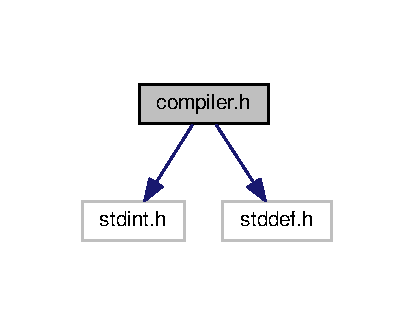
\includegraphics[width=199pt]{compiler_8h__incl}
\end{center}
\end{figure}
This graph shows which files directly or indirectly include this file\-:\nopagebreak
\begin{figure}[H]
\begin{center}
\leavevmode
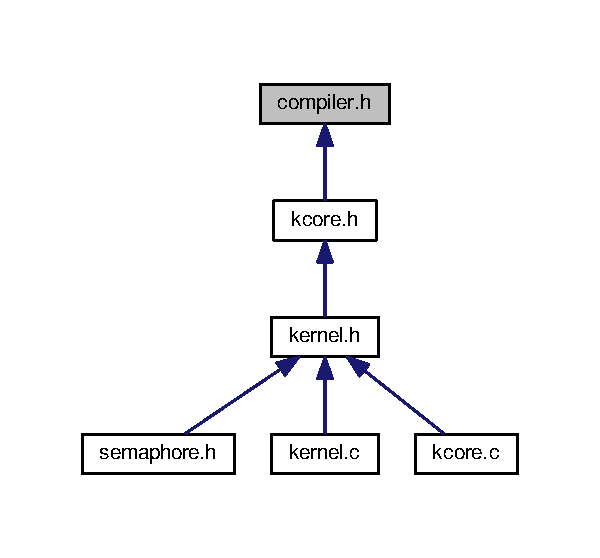
\includegraphics[width=288pt]{compiler_8h__dep__incl}
\end{center}
\end{figure}
\subsubsection*{Macros}
\begin{Indent}{\bf Compiler provided macros}\par
{\em Port interface macros and port specific macros

These macros are used to ease the writing of ports. All macros prefixed with {\bfseries P\-O\-R\-T\-\_\-} are part of the port interface. }\begin{DoxyCompactItemize}
\item 
\#define \hyperlink{group__template__compiler_ga87952d6e574c7f437503926e833ba345}{P\-O\-R\-T\-\_\-\-C\-\_\-\-I\-N\-L\-I\-N\-E}~inline
\begin{DoxyCompactList}\small\item\em C extension -\/ make a function inline. \end{DoxyCompactList}\item 
\#define \hyperlink{group__template__compiler_ga89152d5aab4045f552113b32920741ce}{P\-O\-R\-T\-\_\-\-C\-\_\-\-I\-N\-L\-I\-N\-E\-\_\-\-A\-L\-W\-A\-Y\-S}~inline
\begin{DoxyCompactList}\small\item\em C extension -\/ make a function inline -\/ always. \end{DoxyCompactList}\item 
\#define \hyperlink{group__template__compiler_gaf50b092bb255c796c99927cebbdb8631}{P\-O\-R\-T\-\_\-\-C\-\_\-\-N\-A\-K\-E\-D}
\begin{DoxyCompactList}\small\item\em Omit function prologue/epilogue sequences. \end{DoxyCompactList}\item 
\#define \hyperlink{group__template__compiler_ga6fe63660c6d0ccbabb032c026714863e}{P\-O\-R\-T\-\_\-\-C\-\_\-\-F\-U\-N\-C}~\char`\"{}unknown\char`\"{}
\begin{DoxyCompactList}\small\item\em Provides function name for assert macros. \end{DoxyCompactList}\item 
\#define \hyperlink{group__template__compiler_ga70c3ad4cff78229fae591d039b59f4d1}{P\-O\-R\-T\-\_\-\-C\-\_\-\-W\-E\-A\-K}
\begin{DoxyCompactList}\small\item\em Declares a weak function. \end{DoxyCompactList}\item 
\#define \hyperlink{group__template__compiler_ga4d6b8bd33e54fa5af4c5291c92dda288}{P\-O\-R\-T\-\_\-\-C\-\_\-\-A\-L\-I\-G\-N\-E\-D}(expr)
\begin{DoxyCompactList}\small\item\em This attribute specifies a minimum alignment (in bytes) for variables of the specified type. \end{DoxyCompactList}\item 
\#define \hyperlink{group__template__compiler_ga47fdf2153dba3df8c6a840829f02bd66}{P\-O\-R\-T\-\_\-\-H\-W\-R\-E\-G\-\_\-\-S\-E\-T}(reg, mask, val)
\begin{DoxyCompactList}\small\item\em A standardized way of properly setting the value of H\-W register. \end{DoxyCompactList}\end{DoxyCompactItemize}
\end{Indent}
\subsubsection*{Compiler provided data types}
\label{_amgrp0fa76376c1171116a77221ec211612f0}%
The compiler port must provide some C90 (C99) data types

The compiler port must\-:
\begin{DoxyItemize}
\item declare sets of integer types having specified widths, standard type definitions and shall define corresponding sets of macros.
\end{DoxyItemize}

Types are defined in the following categories\-:
\begin{DoxyItemize}
\item Integer types having certain exact widths
\item Fastest integer types having at least certain specified widths
\item Integer types wide enough to hold pointers to objects
\item standard type definitions
\end{DoxyItemize}

The following exact-\/width integer types are required\-:
\begin{DoxyItemize}
\item int8\-\_\-t
\item int16\-\_\-t
\item int32\-\_\-t
\item uint8\-\_\-t
\item uint16\-\_\-t
\item uint32\-\_\-t
\end{DoxyItemize}

The following fastest minimum-\/width integer types are required\-:
\begin{DoxyItemize}
\item int\-\_\-fast8\-\_\-t
\item int\-\_\-fast16\-\_\-t
\item int\-\_\-fast32\-\_\-t
\item uint\-\_\-fast8\-\_\-t
\item uint\-\_\-fast16\-\_\-t
\item uint\-\_\-fast32\-\_\-t
\end{DoxyItemize}

The following integer types capable of holding object pointers are required\-:
\begin{DoxyItemize}
\item intptr\-\_\-t
\item uintptr\-\_\-t
\end{DoxyItemize}

The following standard type definitions are required\-:
\begin{DoxyItemize}
\item N\-U\-L\-L
\item ptrdiff\-\_\-t
\item size\-\_\-t 
\end{DoxyItemize}\begin{DoxyCompactItemize}
\item 
enum \hyperlink{group__template__compiler_ga05f6c3f21a0d28271ad754637673d8fa}{bool\-Type} \{ \\*
\hyperlink{group__template__compiler_gga05f6c3f21a0d28271ad754637673d8faaa82764c3079aea4e60c80e45befbb839}{T\-R\-U\-E} = 1\-U, 
\\*
\hyperlink{group__template__compiler_gga05f6c3f21a0d28271ad754637673d8faaa1e095cc966dbecf6a0d8aad75348d1a}{F\-A\-L\-S\-E} = 0\-U
 \}
\begin{DoxyCompactList}\small\item\em Bool data type. \end{DoxyCompactList}\item 
typedef enum \hyperlink{group__template__compiler_ga05f6c3f21a0d28271ad754637673d8fa}{bool\-Type} \hyperlink{group__template__compiler_ga74fbee312f9185efb602f89d21b53404}{bool\-\_\-\-T}
\begin{DoxyCompactList}\small\item\em Bool data type. \end{DoxyCompactList}\end{DoxyCompactItemize}


\subsubsection{Detailed Description}
Interface of Compiler port -\/ Template. \begin{DoxyAuthor}{Author}
Nenad Radulovic 
\end{DoxyAuthor}

\hypertarget{kcore_8c}{\subsection{kcore.\-c File Reference}
\label{kcore_8c}\index{kcore.\-c@{kcore.\-c}}
}


Implementation of C\-P\-U port -\/ Template.  


{\ttfamily \#include \char`\"{}kernel/kernel.\-h\char`\"{}}\\*
Include dependency graph for kcore.\-c\-:\nopagebreak
\begin{figure}[H]
\begin{center}
\leavevmode
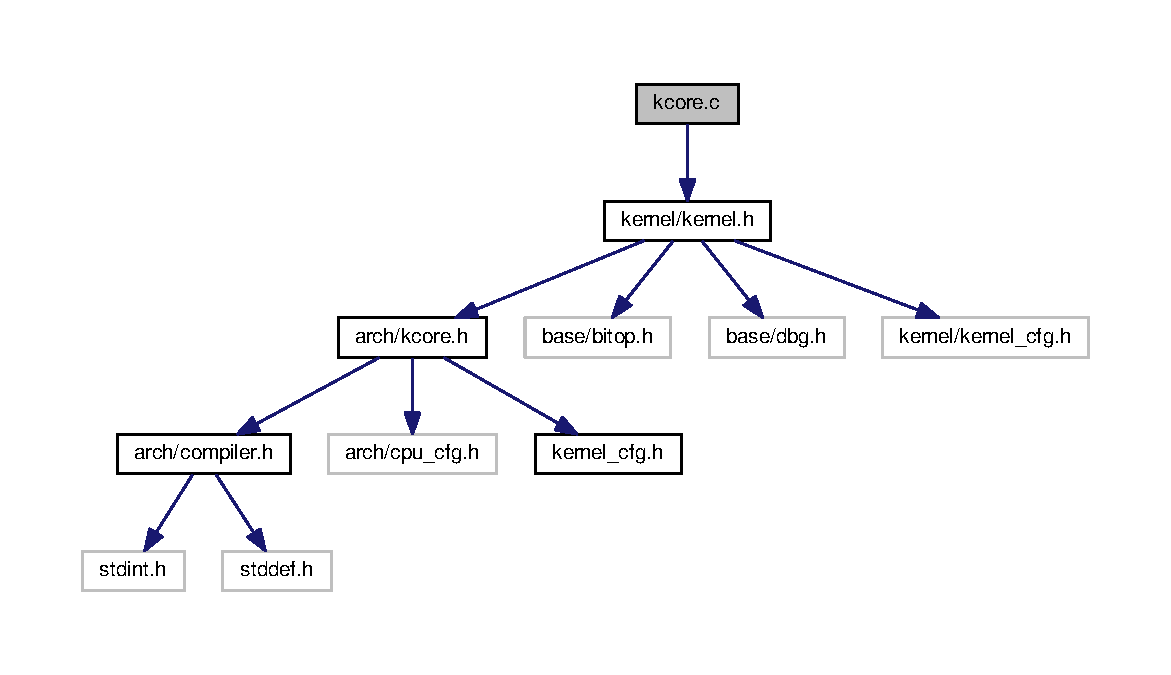
\includegraphics[width=350pt]{kcore_8c__incl}
\end{center}
\end{figure}
\subsubsection*{Functions}
\begin{DoxyCompactItemize}
\item 
void $\ast$ \hyperlink{group__template__cpu__impl_gaa097ec2ead487892969bcd2806539822}{port\-Ctx\-Init} (void $\ast$stck, size\-\_\-t stck\-Size, void($\ast$fn)(void $\ast$), void $\ast$arg)
\begin{DoxyCompactList}\small\item\em Initialize the thread context. \end{DoxyCompactList}\end{DoxyCompactItemize}


\subsubsection{Detailed Description}
Implementation of C\-P\-U port -\/ Template. \begin{DoxyAuthor}{Author}
Nenad Radulovic 
\end{DoxyAuthor}

\hypertarget{kcore_8h}{\subsection{kcore.\-h File Reference}
\label{kcore_8h}\index{kcore.\-h@{kcore.\-h}}
}


Interface of C\-P\-U port -\/ Template.  


{\ttfamily \#include \char`\"{}arch/compiler.\-h\char`\"{}}\\*
{\ttfamily \#include \char`\"{}arch/cpu\-\_\-cfg.\-h\char`\"{}}\\*
{\ttfamily \#include \char`\"{}kernel\-\_\-cfg.\-h\char`\"{}}\\*
Include dependency graph for kcore.\-h\-:\nopagebreak
\begin{figure}[H]
\begin{center}
\leavevmode
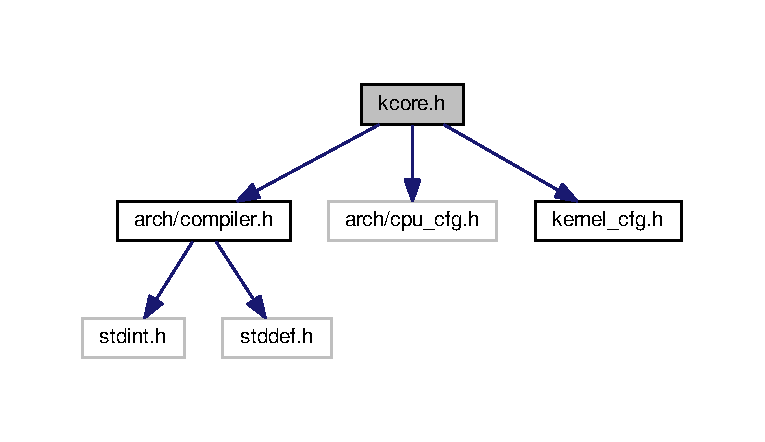
\includegraphics[width=350pt]{kcore_8h__incl}
\end{center}
\end{figure}
This graph shows which files directly or indirectly include this file\-:\nopagebreak
\begin{figure}[H]
\begin{center}
\leavevmode
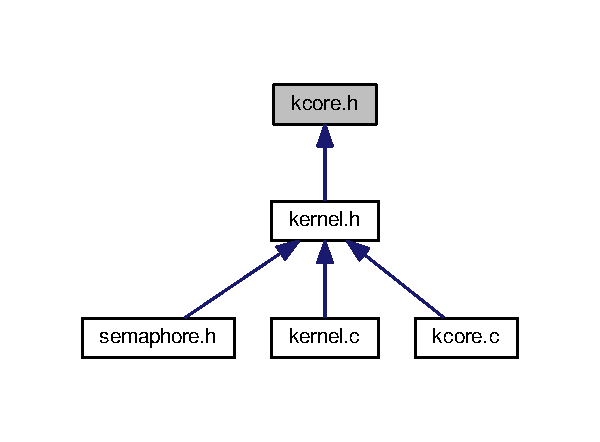
\includegraphics[width=288pt]{kcore_8h__dep__incl}
\end{center}
\end{figure}
\subsubsection*{Data Structures}
\begin{DoxyCompactItemize}
\item 
struct \hyperlink{structportStck}{port\-Stck}
\begin{DoxyCompactList}\small\item\em Stack structure used for stack declaration in order to force the alignment Alignment of stack structure. \end{DoxyCompactList}\item 
struct \hyperlink{structportCtx}{port\-Ctx}
\begin{DoxyCompactList}\small\item\em Port context structure. \end{DoxyCompactList}\end{DoxyCompactItemize}
\subsubsection*{Macros}
\begin{Indent}{\bf Port constants}\par
\begin{DoxyCompactItemize}
\item 
\#define \hyperlink{group__template__cpu__intf_ga5a629fee11006b5b0b97f7cb7176efd4}{P\-O\-R\-T\-\_\-\-D\-E\-F\-\_\-\-S\-T\-C\-K\-\_\-\-M\-I\-N\-S\-I\-Z\-E}~(sizeof(struct \hyperlink{structportCtx}{port\-Ctx}) / sizeof(port\-Reg\-\_\-\-T))
\begin{DoxyCompactList}\small\item\em This macro specifies the minimal size of the thread stack. \end{DoxyCompactList}\end{DoxyCompactItemize}
\end{Indent}
\begin{Indent}{\bf System timer constants}\par
\begin{DoxyCompactItemize}
\item 
\#define \hyperlink{group__template__cpu__intf_ga96e15dd16b285b0feb6e225b0834ad10}{P\-O\-R\-T\-\_\-\-D\-E\-F\-\_\-\-S\-Y\-S\-T\-M\-R\-\_\-\-W\-A\-K\-E\-U\-P\-\_\-\-T\-H\-\_\-\-V\-A\-L}~600u
\begin{DoxyCompactList}\small\item\em Threshold system timer value for new tick. \end{DoxyCompactList}\end{DoxyCompactItemize}
\end{Indent}
\begin{Indent}{\bf Kernel threads port dependent settings}\par
{\em Kernel uses several threads for system management. This section defines port dependent settings for the threads. }\begin{DoxyCompactItemize}
\item 
\#define \hyperlink{group__template__cpu__intf_gabaa296d76c28043a60531ad8ed81504b}{P\-O\-R\-T\-\_\-\-D\-E\-F\-\_\-\-K\-V\-T\-M\-R\-\_\-\-S\-T\-C\-K\-\_\-\-S\-I\-Z\-E}~40u
\begin{DoxyCompactList}\small\item\em Kernel Virtual Timer Thread stack size. \end{DoxyCompactList}\item 
\#define \hyperlink{group__template__cpu__intf_ga31d47ffb78c3755575e66821b3a72a62}{P\-O\-R\-T\-\_\-\-D\-E\-F\-\_\-\-K\-I\-D\-L\-E\-\_\-\-S\-T\-C\-K\-\_\-\-S\-I\-Z\-E}~40u
\begin{DoxyCompactList}\small\item\em Kernel Idle Thread stack size. \end{DoxyCompactList}\end{DoxyCompactItemize}
\end{Indent}
\begin{Indent}{\bf Interrupt management}\par
{\em P\-O\-R\-T\-\_\-\-I\-S\-R\-\_\-... macros are used by es\-Kern\-Isr\-Enter() and es\-Kern\-Isr\-Exit() functions. They are used to keep the current level of I\-S\-R nesting. Scheduler should be invoked only from the last I\-S\-R that is executing. }\begin{DoxyCompactItemize}
\item 
\#define \hyperlink{group__template__cpu__intf_gaccad9298c874b29753b318d4f900cb75}{P\-O\-R\-T\-\_\-\-I\-S\-R\-\_\-\-E\-N\-T\-E\-R}()
\begin{DoxyCompactList}\small\item\em Enter I\-S\-R. Increment Port\-Isr\-Nesting variable to keep track of I\-S\-R nesting. \end{DoxyCompactList}\item 
\#define \hyperlink{group__template__cpu__intf_ga267c312d7321e9361b454f4274bbc087}{P\-O\-R\-T\-\_\-\-I\-S\-R\-\_\-\-E\-X\-I\-T}()
\begin{DoxyCompactList}\small\item\em Exit I\-S\-R. Decrement Port\-Isr\-Nesting variable to keep track of I\-S\-R nesting. \end{DoxyCompactList}\item 
\#define \hyperlink{group__template__cpu__intf_ga6c0ea20c8e1f6b9751f51916da8e2aee}{P\-O\-R\-T\-\_\-\-I\-S\-R\-\_\-\-I\-S\-\_\-\-L\-A\-S\-T}()~(0u == Port\-Isr\-Nesting ? T\-R\-U\-E \-: F\-A\-L\-S\-E)
\begin{DoxyCompactList}\small\item\em If isr\-Nesting variable is zero then the last I\-S\-R is executing and scheduler should be invoked. \end{DoxyCompactList}\end{DoxyCompactItemize}
\end{Indent}
\begin{Indent}{\bf General port macros}\par
\begin{DoxyCompactItemize}
\item 
\#define \hyperlink{group__template__cpu__intf_gabf0ea7d36355a7133ee9e9f8abafa6ff}{P\-O\-R\-T\-\_\-\-K\-C\-O\-R\-E\-\_\-\-I\-N\-I\-T\-\_\-\-E\-A\-R\-L\-Y}()
\begin{DoxyCompactList}\small\item\em Early port initialization. \end{DoxyCompactList}\item 
\#define \hyperlink{group__template__cpu__intf_ga682a913f5439544d4f0ee14ae68507fd}{P\-O\-R\-T\-\_\-\-K\-C\-O\-R\-E\-\_\-\-I\-N\-I\-T}()
\begin{DoxyCompactList}\small\item\em Port initialization. \end{DoxyCompactList}\item 
\#define \hyperlink{group__template__cpu__intf_ga5c133105168261f1744abf3c5917a515}{P\-O\-R\-T\-\_\-\-K\-C\-O\-R\-E\-\_\-\-I\-N\-I\-T\-\_\-\-L\-A\-T\-E}()
\begin{DoxyCompactList}\small\item\em Late port initialization. \end{DoxyCompactList}\item 
\#define \hyperlink{group__template__cpu__intf_gac386e206a8b5225c9aa56be88b625837}{P\-O\-R\-T\-\_\-\-K\-C\-O\-R\-E\-\_\-\-T\-E\-R\-M}()
\begin{DoxyCompactList}\small\item\em Terminate port. \end{DoxyCompactList}\item 
\#define \hyperlink{group__template__cpu__intf_gacb3a46e89d327fbaf5c122fe23877b24}{P\-O\-R\-T\-\_\-\-S\-T\-C\-K\-\_\-\-S\-I\-Z\-E}(size)~(size + \hyperlink{group__template__cpu__intf_ga5a629fee11006b5b0b97f7cb7176efd4}{P\-O\-R\-T\-\_\-\-D\-E\-F\-\_\-\-S\-T\-C\-K\-\_\-\-M\-I\-N\-S\-I\-Z\-E})
\begin{DoxyCompactList}\small\item\em Calculate the stack size. \end{DoxyCompactList}\item 
\#define \hyperlink{group__template__cpu__intf_gad699a79233d442ae90a69c113e314542}{P\-O\-R\-T\-\_\-\-C\-R\-I\-T\-I\-C\-A\-L\-\_\-\-E\-X\-I\-T\-\_\-\-S\-L\-E\-E\-P}()~port\-Int\-Set\-Sleep\-Enter\-\_\-(int\-Status\-\_\-)
\begin{DoxyCompactList}\small\item\em Exit critical section and enter sleep state. \end{DoxyCompactList}\end{DoxyCompactItemize}
\end{Indent}
\subsubsection*{Typedefs}
\begin{DoxyCompactItemize}
\item 
typedef struct \hyperlink{structportStck}{port\-Stck} \hyperlink{group__template__cpu__intf_ga13cc91970e3e05fe4210440c068d3f4a}{port\-Stck\-\_\-\-T}
\begin{DoxyCompactList}\small\item\em Stack type. \end{DoxyCompactList}\end{DoxyCompactItemize}
\subsubsection*{Variables}
\begin{DoxyCompactItemize}
\item 
port\-Reg\-\_\-\-T \hyperlink{group__template__cpu__intf_gab0ad3c664e66a9a334daa4109c14e585}{Port\-Isr\-Nesting}
\begin{DoxyCompactList}\small\item\em Variable to keep track of I\-S\-R nesting. \end{DoxyCompactList}\end{DoxyCompactItemize}
\subsubsection*{Dispatcher context switching}
\begin{DoxyCompactItemize}
\item 
\#define \hyperlink{group__template__cpu__intf_ga80d15a56d61c9d4e786e52006ff4ac43}{P\-O\-R\-T\-\_\-\-C\-T\-X\-\_\-\-I\-N\-I\-T}(stck, stack\-Size, thread, arg)
\begin{DoxyCompactList}\small\item\em Initialize the thread context. \end{DoxyCompactList}\item 
\#define \hyperlink{group__template__cpu__intf_ga50a3b72a7f2065922811f0d6dedda01a}{P\-O\-R\-T\-\_\-\-C\-T\-X\-\_\-\-S\-W}()
\begin{DoxyCompactList}\small\item\em Do the context switch -\/ invoked from A\-P\-I level. \end{DoxyCompactList}\item 
\#define \hyperlink{group__template__cpu__intf_ga20bba8f9c5a2f38fd7c63b9d2320e511}{P\-O\-R\-T\-\_\-\-C\-T\-X\-\_\-\-S\-W\-\_\-\-I\-S\-R}()
\begin{DoxyCompactList}\small\item\em Do the context switch -\/ invoked from I\-S\-R level. \end{DoxyCompactList}\item 
\#define \hyperlink{group__template__cpu__intf_ga58056289ebeda87723f99f5431c6239e}{P\-O\-R\-T\-\_\-\-C\-T\-X\-\_\-\-S\-W\-\_\-\-S\-T\-A\-R\-T}()
\begin{DoxyCompactList}\small\item\em Start the first thread. \end{DoxyCompactList}\item 
void $\ast$ \hyperlink{group__template__cpu__intf_gaa097ec2ead487892969bcd2806539822}{port\-Ctx\-Init} (void $\ast$stck, size\-\_\-t stck\-Size, void($\ast$fn)(void $\ast$), void $\ast$arg)
\begin{DoxyCompactList}\small\item\em Initialize the thread context. \end{DoxyCompactList}\end{DoxyCompactItemize}


\subsubsection{Detailed Description}
Interface of C\-P\-U port -\/ Template. \begin{DoxyAuthor}{Author}
Nenad Radulovic 
\end{DoxyAuthor}

\hypertarget{kernel-example_8dox}{\subsection{kernel-\/example.dox File Reference}
\label{kernel-example_8dox}\index{kernel-\/example.\-dox@{kernel-\/example.\-dox}}
}

\hypertarget{kernel_8c}{\subsection{kernel.\-c File Reference}
\label{kernel_8c}\index{kernel.\-c@{kernel.\-c}}
}


Implementation of kernel port independent code.  


{\ttfamily \#include \char`\"{}kernel/kernel.\-h\char`\"{}}\\*
{\ttfamily \#include \char`\"{}base/critical.\-h\char`\"{}}\\*
Include dependency graph for kernel.\-c\-:\nopagebreak
\begin{figure}[H]
\begin{center}
\leavevmode
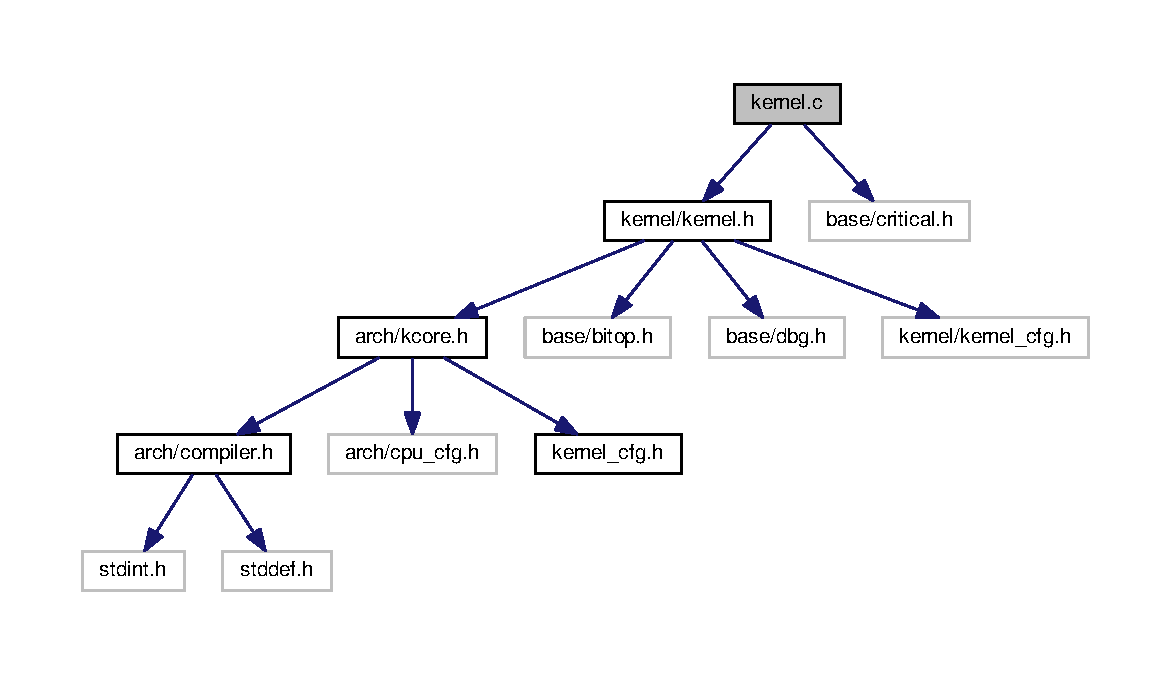
\includegraphics[width=350pt]{kernel_8c__incl}
\end{center}
\end{figure}
\subsubsection*{Data Structures}
\begin{DoxyCompactItemize}
\item 
struct \hyperlink{structsysTmr}{sys\-Tmr}
\begin{DoxyCompactList}\small\item\em Main System Timer structure. \end{DoxyCompactList}\end{DoxyCompactItemize}
\subsubsection*{Macros}
\begin{DoxyCompactItemize}
\item 
\#define \hyperlink{group__kern__impl_ga8558d079ebfe8a9af11fc796d46d9ab5}{D\-E\-F\-\_\-\-S\-C\-H\-E\-D\-\_\-\-S\-T\-A\-T\-E\-\_\-\-I\-N\-T\-S\-R\-V\-\_\-\-M\-S\-K}~(0x01u $<$$<$ 0)
\begin{DoxyCompactList}\small\item\em Kernel state variable bit position which defines if the kernel is in interrupt servicing state. \end{DoxyCompactList}\item 
\#define \hyperlink{group__kern__impl_gaaf8217f5d1bfca8caecc2206fa74abc7}{D\-E\-F\-\_\-\-S\-C\-H\-E\-D\-\_\-\-S\-T\-A\-T\-E\-\_\-\-L\-O\-C\-K\-\_\-\-M\-S\-K}~(0x01u $<$$<$ 1)
\begin{DoxyCompactList}\small\item\em Kernel state variable bit position which defines if the kernel is locked or not. \end{DoxyCompactList}\item 
\#define \hyperlink{group__kern__impl_ga19da32f7a4f44e5a4bddb5a588d73677}{D\-E\-F\-\_\-\-T\-H\-D\-\_\-\-C\-O\-N\-T\-R\-A\-C\-T\-\_\-\-S\-I\-G\-N\-A\-T\-U\-R\-E}~((port\-Reg\-\_\-\-T)0xfeedbeeful)
\begin{DoxyCompactList}\small\item\em Thread structure signature. \end{DoxyCompactList}\item 
\#define \hyperlink{group__kern__impl_ga7f087a59efb2fe7078a7479aa674b7b4}{D\-E\-F\-\_\-\-T\-H\-D\-Q\-\_\-\-C\-O\-N\-T\-R\-A\-C\-T\-\_\-\-S\-I\-G\-N\-A\-T\-U\-R\-E}~((port\-Reg\-\_\-\-T)0xfeedbef0ul)
\begin{DoxyCompactList}\small\item\em Thread Queue structure signature. \end{DoxyCompactList}\item 
\#define \hyperlink{group__kern__impl_gaed6b30b1e098b37a398f58e2a5b73b8b}{D\-E\-F\-\_\-\-V\-T\-M\-R\-\_\-\-C\-O\-N\-T\-R\-A\-C\-T\-\_\-\-S\-I\-G\-N\-A\-T\-U\-R\-E}~((port\-Reg\-\_\-\-T)0xfeedbef1ul)
\begin{DoxyCompactList}\small\item\em Timer structure signature. \end{DoxyCompactList}\item 
\#define \hyperlink{group__kern__impl_ga177fc11d78c08db1f70168bf971e0059}{D\-L\-I\-S\-T\-\_\-\-I\-S\-\_\-\-E\-N\-T\-R\-Y\-\_\-\-F\-I\-R\-S\-T}(list, entry)~((entry) == (entry)-\/$>$list.\-next)
\begin{DoxyCompactList}\small\item\em D\-List macro\-: is the thread the first one in the list. \end{DoxyCompactList}\item 
\#define \hyperlink{group__kern__impl_gaad48325fff9eb7b4c41788e190a28cf2}{D\-L\-I\-S\-T\-\_\-\-I\-S\-\_\-\-E\-N\-T\-R\-Y\-\_\-\-L\-A\-S\-T}(list, entry)~\hyperlink{group__kern__impl_ga177fc11d78c08db1f70168bf971e0059}{D\-L\-I\-S\-T\-\_\-\-I\-S\-\_\-\-E\-N\-T\-R\-Y\-\_\-\-F\-I\-R\-S\-T}(list, entry)
\begin{DoxyCompactList}\small\item\em D\-List macro\-: is the thread the last one in the list. \end{DoxyCompactList}\item 
\#define \hyperlink{group__kern__impl_ga77e64b5c52cb61e2bb7f6a4c6b0c9acc}{D\-L\-I\-S\-T\-\_\-\-I\-S\-\_\-\-E\-N\-T\-R\-Y\-\_\-\-S\-I\-N\-G\-L\-E}(list, entry)~\hyperlink{group__kern__impl_ga177fc11d78c08db1f70168bf971e0059}{D\-L\-I\-S\-T\-\_\-\-I\-S\-\_\-\-E\-N\-T\-R\-Y\-\_\-\-F\-I\-R\-S\-T}(list, entry)
\begin{DoxyCompactList}\small\item\em D\-List macro\-: is the thread single in the list. \end{DoxyCompactList}\item 
\#define \hyperlink{group__kern__impl_gab4b1b58e436cff32fc080493dfa35619}{D\-L\-I\-S\-T\-\_\-\-E\-N\-T\-R\-Y\-\_\-\-N\-E\-X\-T}(list, entry)~(entry)-\/$>$list.\-next
\begin{DoxyCompactList}\small\item\em D\-List macro\-: get the next entry. \end{DoxyCompactList}\item 
\#define \hyperlink{group__kern__impl_ga23a7667839eb576ddc4f55f2fcf77d65}{D\-L\-I\-S\-T\-\_\-\-E\-N\-T\-R\-Y\-\_\-\-I\-N\-I\-T}(list, entry)
\begin{DoxyCompactList}\small\item\em D\-List macro\-: initialize entry. \end{DoxyCompactList}\item 
\#define \hyperlink{group__kern__impl_gaff514b213c2cd3ad388fd5479275834f}{D\-L\-I\-S\-T\-\_\-\-E\-N\-T\-R\-Y\-\_\-\-A\-D\-D\-\_\-\-A\-F\-T\-E\-R}(list, current, entry)
\begin{DoxyCompactList}\small\item\em D\-List macro\-: add new {\ttfamily entry} after {\ttfamily current} entry. \end{DoxyCompactList}\item 
\#define \hyperlink{group__kern__impl_ga4a663d16206e95f1084af0a44e8518a0}{D\-L\-I\-S\-T\-\_\-\-E\-N\-T\-R\-Y\-\_\-\-R\-M}(list, entry)
\begin{DoxyCompactList}\small\item\em D\-List macro\-: remove the {\ttfamily entry} from a list. \end{DoxyCompactList}\end{DoxyCompactItemize}
\subsubsection*{Functions}
\begin{DoxyCompactItemize}
\item 
\hyperlink{group__kern__impl_ga52b5266d709bc1ce3ca9b1838f389023}{D\-E\-C\-L\-\_\-\-M\-O\-D\-U\-L\-E\-\_\-\-I\-N\-F\-O} (\char`\"{}Kernel\char`\"{}, E\-S\-\_\-\-K\-E\-R\-N\-\_\-\-I\-D,\char`\"{}Nenad Radulovic\char`\"{})
\begin{DoxyCompactList}\small\item\em Module identification info. \end{DoxyCompactList}\item 
void \hyperlink{group__kern__impl_ga9e9ff699d62d6035cd51121bb3140704}{es\-Kern\-Init} (void)
\begin{DoxyCompactList}\small\item\em Initialize kernel internal data structures. \end{DoxyCompactList}\item 
P\-O\-R\-T\-\_\-\-C\-\_\-\-N\-O\-R\-E\-T\-U\-R\-N void \hyperlink{group__kern__impl_ga0e7a0a6b9c02df58de0f98de0229a09d}{es\-Kern\-Start} (void)
\begin{DoxyCompactList}\small\item\em Start the multi-\/threading. \end{DoxyCompactList}\item 
void \hyperlink{group__kern__impl_ga3182e4c1a47897109d0a429b10a2483e}{es\-Kern\-Sys\-Tmr} (void)
\begin{DoxyCompactList}\small\item\em Process the system timer event. \end{DoxyCompactList}\item 
void \hyperlink{group__kern__impl_gac0d578bcd4a10b2c8e5fc90f0b86ccec}{es\-Kern\-Isr\-Enter\-I} (void)
\begin{DoxyCompactList}\small\item\em Enter Interrupt Service Routine. \end{DoxyCompactList}\item 
void \hyperlink{group__kern__impl_gaa6347925fff1684b5425dd2857c27129}{es\-Kern\-Isr\-Exit\-I} (void)
\begin{DoxyCompactList}\small\item\em Exit Interrupt Service Routine. \end{DoxyCompactList}\item 
void \hyperlink{group__kern__impl_gaa3ca4a02fafcfb840442506f42175a13}{es\-Kern\-Lock\-Int\-Enter} (\hyperlink{group__kern__lock_gad8b2b8257c3bf42c064adb66c0d45e2e}{es\-Lock\-Ctx\-\_\-\-T} $\ast$lock\-Ctx)
\begin{DoxyCompactList}\small\item\em Enter a critical code lock. \end{DoxyCompactList}\item 
void \hyperlink{group__kern__impl_gad8cb192a48802804cc12162edd18668d}{es\-Kern\-Lock\-Int\-Exit} (\hyperlink{group__kern__lock_gad8b2b8257c3bf42c064adb66c0d45e2e}{es\-Lock\-Ctx\-\_\-\-T} lock\-Ctx)
\begin{DoxyCompactList}\small\item\em Exit a critical code lock. \end{DoxyCompactList}\item 
void \hyperlink{group__kern__impl_ga6dd45355c20a10f7272bd39670353428}{es\-Kern\-Lock\-Enter\-I} (void)
\begin{DoxyCompactList}\small\item\em Lock the scheduler. \end{DoxyCompactList}\item 
void \hyperlink{group__kern__impl_ga3287aefb2c7dd24672c716d86a008ad3}{es\-Kern\-Lock\-Exit\-I} (void)
\begin{DoxyCompactList}\small\item\em Unlock the scheduler. \end{DoxyCompactList}\item 
void \hyperlink{group__kern__impl_ga86ec4f4cbaa889b0f23c7e2ebdcbbb97}{es\-Kern\-Lock\-Enter} (void)
\begin{DoxyCompactList}\small\item\em Lock the scheduler. \end{DoxyCompactList}\item 
void \hyperlink{group__kern__impl_gaf1eec663f7cc5c414b113901382ccd82}{es\-Kern\-Lock\-Exit} (void)
\begin{DoxyCompactList}\small\item\em Unlock the scheduler. \end{DoxyCompactList}\item 
void \hyperlink{group__kern__impl_gac91734f3ee867b519f59bf81cc7fde88}{es\-Thd\-Init} (\hyperlink{group__kern__thd_ga62e3a3ca0a4597a19c43cb8868810d82}{es\-Thd\-\_\-\-T} $\ast$thd, void($\ast$fn)(void $\ast$), void $\ast$arg, \hyperlink{group__template__cpu__intf_ga13cc91970e3e05fe4210440c068d3f4a}{port\-Stck\-\_\-\-T} $\ast$stck, size\-\_\-t stck\-Size, uint8\-\_\-t prio)
\begin{DoxyCompactList}\small\item\em Initialize the specified thread. \end{DoxyCompactList}\item 
void \hyperlink{group__kern__impl_gac9d1eac76f26096614e8196bcfd8b905}{es\-Thd\-Term} (\hyperlink{group__kern__thd_ga62e3a3ca0a4597a19c43cb8868810d82}{es\-Thd\-\_\-\-T} $\ast$thd)
\begin{DoxyCompactList}\small\item\em Terminate the specified thread. \end{DoxyCompactList}\item 
void \hyperlink{group__kern__impl_ga8eaa731d0026a8a1667d4422d5031df6}{es\-Thd\-Set\-Prio\-I} (\hyperlink{group__kern__thd_ga62e3a3ca0a4597a19c43cb8868810d82}{es\-Thd\-\_\-\-T} $\ast$thd, uint8\-\_\-t prio)
\begin{DoxyCompactList}\small\item\em Set the priority of a thread. \end{DoxyCompactList}\item 
void \hyperlink{group__kern__impl_gaddd5fe0557c91559b9452beb0fc236fd}{es\-Thd\-Q\-Init} (\hyperlink{group__kern__thdq_ga7a1a060699e83a01512ebb5540019556}{es\-Thd\-Q\-\_\-\-T} $\ast$thd\-Q)
\begin{DoxyCompactList}\small\item\em Initialize Thread Queue. \end{DoxyCompactList}\item 
void \hyperlink{group__kern__impl_gaa5f19b32a7f0c42616b5270dcbd73a3e}{es\-Thd\-Q\-Term} (\hyperlink{group__kern__thdq_ga7a1a060699e83a01512ebb5540019556}{es\-Thd\-Q\-\_\-\-T} $\ast$thd\-Q)
\begin{DoxyCompactList}\small\item\em Terminate Thread Queue. \end{DoxyCompactList}\item 
void \hyperlink{group__kern__impl_ga9da1e71c137d8adb8c9bdead7052b5fa}{es\-Thd\-Q\-Add\-I} (\hyperlink{group__kern__thdq_ga7a1a060699e83a01512ebb5540019556}{es\-Thd\-Q\-\_\-\-T} $\ast$thd\-Q, \hyperlink{group__kern__thd_ga62e3a3ca0a4597a19c43cb8868810d82}{es\-Thd\-\_\-\-T} $\ast$thd)
\begin{DoxyCompactList}\small\item\em Add a thread to the Thread Queue. \end{DoxyCompactList}\item 
void \hyperlink{group__kern__impl_gaa18afa95e34035da03c5cb7ea3a96320}{es\-Thd\-Q\-Rm\-I} (\hyperlink{group__kern__thdq_ga7a1a060699e83a01512ebb5540019556}{es\-Thd\-Q\-\_\-\-T} $\ast$thd\-Q, \hyperlink{group__kern__thd_ga62e3a3ca0a4597a19c43cb8868810d82}{es\-Thd\-\_\-\-T} $\ast$thd)
\begin{DoxyCompactList}\small\item\em Removes the thread from the Thread Queue. \end{DoxyCompactList}\item 
\hyperlink{group__kern__thd_ga62e3a3ca0a4597a19c43cb8868810d82}{es\-Thd\-\_\-\-T} $\ast$ \hyperlink{group__kern__impl_ga1670c123f31c346b24ec9d2b7ae35f88}{es\-Thd\-Q\-Fetch\-I} (const \hyperlink{group__kern__thdq_ga7a1a060699e83a01512ebb5540019556}{es\-Thd\-Q\-\_\-\-T} $\ast$thd\-Q)
\begin{DoxyCompactList}\small\item\em Fetch the first high priority thread from the Thread Queue. \end{DoxyCompactList}\item 
\hyperlink{group__kern__thd_ga62e3a3ca0a4597a19c43cb8868810d82}{es\-Thd\-\_\-\-T} $\ast$ \hyperlink{group__kern__impl_gae365b14292f1496a90d876baec84fb4e}{es\-Thd\-Q\-Fetch\-Rotate\-I} (\hyperlink{group__kern__thdq_ga7a1a060699e83a01512ebb5540019556}{es\-Thd\-Q\-\_\-\-T} $\ast$thd\-Q, uint\-\_\-fast8\-\_\-t prio)
\begin{DoxyCompactList}\small\item\em Fetch the next thread and rotate thread linked list. \end{DoxyCompactList}\item 
\hyperlink{group__template__compiler_ga74fbee312f9185efb602f89d21b53404}{bool\-\_\-\-T} \hyperlink{group__kern__impl_gacf2687b82ce64e2154d97fd3b69a4ab5}{es\-Thd\-Q\-Is\-Empty} (const \hyperlink{group__kern__thdq_ga7a1a060699e83a01512ebb5540019556}{es\-Thd\-Q\-\_\-\-T} $\ast$thd\-Q)
\begin{DoxyCompactList}\small\item\em Is thread queue empty. \end{DoxyCompactList}\item 
void \hyperlink{group__kern__impl_ga73e14b1860ce824c822adc407aee0977}{es\-Sched\-Rdy\-Add\-I} (\hyperlink{group__kern__thd_ga62e3a3ca0a4597a19c43cb8868810d82}{es\-Thd\-\_\-\-T} $\ast$thd)
\begin{DoxyCompactList}\small\item\em Add thread {\ttfamily thd} to the ready thread list and notify the scheduler. \end{DoxyCompactList}\item 
void \hyperlink{group__kern__impl_ga0b8263c5024ebb59cd9b95cc9253b44d}{es\-Sched\-Rdy\-Rm\-I} (\hyperlink{group__kern__thd_ga62e3a3ca0a4597a19c43cb8868810d82}{es\-Thd\-\_\-\-T} $\ast$thd)
\begin{DoxyCompactList}\small\item\em Remove thread {\ttfamily thd} from the ready thread list and notify the scheduler. \end{DoxyCompactList}\item 
void \hyperlink{group__kern__impl_gaf90e487bfce974dafaeed5009e189810}{es\-Sched\-Yield\-I} (void)
\begin{DoxyCompactList}\small\item\em Force the scheduler invocation which will evaluate all ready threads and switch to ready thread with the highest priority. \end{DoxyCompactList}\item 
void \hyperlink{group__kern__impl_gafbea29b376b29f11bbfc48a0f5144e9a}{es\-Sched\-Yield\-Isr\-I} (void)
\begin{DoxyCompactList}\small\item\em Force the scheduler invocation which will evaluate all ready threads and switch to ready thread with the highest priority. \end{DoxyCompactList}\item 
void \hyperlink{group__kern__impl_ga45fe650eac73e7fe203cc81565401555}{es\-V\-Tmr\-Init\-I} (\hyperlink{group__kern__vtmr_ga3c020f0ca54ff412bc1d1505502d2afc}{es\-V\-Tmr\-\_\-\-T} $\ast$v\-Tmr, \hyperlink{group__kern__vtmr_ga844873888c186ee81eb66620dadb0451}{es\-Tick\-\_\-\-T} tick, void($\ast$fn)(void $\ast$), void $\ast$arg)
\begin{DoxyCompactList}\small\item\em Add and start a new virtual timer. \end{DoxyCompactList}\item 
void \hyperlink{group__kern__impl_gad932cf00aec4ba03a0df02ccc493c4c2}{es\-V\-Tmr\-Init} (\hyperlink{group__kern__vtmr_ga3c020f0ca54ff412bc1d1505502d2afc}{es\-V\-Tmr\-\_\-\-T} $\ast$v\-Tmr, \hyperlink{group__kern__vtmr_ga844873888c186ee81eb66620dadb0451}{es\-Tick\-\_\-\-T} tick, void($\ast$fn)(void $\ast$), void $\ast$arg)
\begin{DoxyCompactList}\small\item\em Add and start a new virtual timer. \end{DoxyCompactList}\item 
void \hyperlink{group__kern__impl_ga96bb2c81f649c0305dfd08d1c79b2e37}{es\-V\-Tmr\-Term\-I} (\hyperlink{group__kern__vtmr_ga3c020f0ca54ff412bc1d1505502d2afc}{es\-V\-Tmr\-\_\-\-T} $\ast$v\-Tmr)
\begin{DoxyCompactList}\small\item\em Cancel and remove a virtual timer. \end{DoxyCompactList}\item 
void \hyperlink{group__kern__impl_gad6ec93a68e3526f18ed926cd441878cd}{es\-V\-Tmr\-Term} (\hyperlink{group__kern__vtmr_ga3c020f0ca54ff412bc1d1505502d2afc}{es\-V\-Tmr\-\_\-\-T} $\ast$v\-Tmr)
\begin{DoxyCompactList}\small\item\em Cancel and remove a virtual timer. \end{DoxyCompactList}\item 
void \hyperlink{group__kern__impl_ga26d10c6aaa0cd1d04261d2c9911e890d}{es\-V\-Tmr\-Delay} (\hyperlink{group__kern__vtmr_ga844873888c186ee81eb66620dadb0451}{es\-Tick\-\_\-\-T} tick)
\begin{DoxyCompactList}\small\item\em Delay for specified amount of ticks. \end{DoxyCompactList}\item 
\hyperlink{group__kern__vtmr_ga844873888c186ee81eb66620dadb0451}{es\-Tick\-\_\-\-T} \hyperlink{group__kern__impl_gacb0d88d6a7e467dc37a6a9a85945aaa6}{es\-Sys\-Tmr\-Tick\-Get} (void)
\begin{DoxyCompactList}\small\item\em Get the current tick value. \end{DoxyCompactList}\end{DoxyCompactItemize}
\begin{Indent}{\bf Priority Bit Map}\par
\begin{DoxyCompactItemize}
\item 
static \hyperlink{group__template__compiler_ga87952d6e574c7f437503926e833ba345}{P\-O\-R\-T\-\_\-\-C\-\_\-\-I\-N\-L\-I\-N\-E} void \hyperlink{group__kern__impl_gaccc724ae39d88a6fcf21891c390ea845}{pbm\-Init} (struct pbm\-\_\- $\ast$pbm)
\begin{DoxyCompactList}\small\item\em Initialize bitmap. \end{DoxyCompactList}\item 
static \hyperlink{group__template__compiler_ga87952d6e574c7f437503926e833ba345}{P\-O\-R\-T\-\_\-\-C\-\_\-\-I\-N\-L\-I\-N\-E} void \hyperlink{group__kern__impl_gabd45c91981a68e1b23c765e8eb59b07b}{pbm\-Set} (struct pbm\-\_\- $\ast$pbm, uint\-\_\-fast8\-\_\-t prio)
\begin{DoxyCompactList}\small\item\em Set the bit corresponding to the prio argument. \end{DoxyCompactList}\item 
static \hyperlink{group__template__compiler_ga87952d6e574c7f437503926e833ba345}{P\-O\-R\-T\-\_\-\-C\-\_\-\-I\-N\-L\-I\-N\-E} void \hyperlink{group__kern__impl_ga53b46c788cfe6e4cc27ee6a3b6c1dfea}{pbm\-Clear} (struct pbm\-\_\- $\ast$pbm, uint\-\_\-fast8\-\_\-t prio)
\begin{DoxyCompactList}\small\item\em Clear the bit corresponding to the prio argument. \end{DoxyCompactList}\item 
static \hyperlink{group__template__compiler_ga87952d6e574c7f437503926e833ba345}{P\-O\-R\-T\-\_\-\-C\-\_\-\-I\-N\-L\-I\-N\-E} uint\-\_\-fast8\-\_\-t \hyperlink{group__kern__impl_ga126e2a40ac85cba9f8ce32b803cb8906}{pbm\-Get\-Highest} (const struct pbm\-\_\- $\ast$pbm)
\begin{DoxyCompactList}\small\item\em Get the highest priority set. \end{DoxyCompactList}\item 
static \hyperlink{group__template__compiler_ga87952d6e574c7f437503926e833ba345}{P\-O\-R\-T\-\_\-\-C\-\_\-\-I\-N\-L\-I\-N\-E} \hyperlink{group__template__compiler_ga74fbee312f9185efb602f89d21b53404}{bool\-\_\-\-T} \hyperlink{group__kern__impl_gae681fb07746d91e97533dfcd9d7b9a9c}{pbm\-Is\-Empty} (const struct pbm\-\_\- $\ast$pbm)
\begin{DoxyCompactList}\small\item\em Is bit map empty? \end{DoxyCompactList}\end{DoxyCompactItemize}
\end{Indent}
\begin{Indent}{\bf Virtual Timer and Virtual Timer kernel thread}\par
\begin{DoxyCompactItemize}
\item 
static \hyperlink{group__template__compiler_ga87952d6e574c7f437503926e833ba345}{P\-O\-R\-T\-\_\-\-C\-\_\-\-I\-N\-L\-I\-N\-E} void \hyperlink{group__kern__impl_ga6ebc5795dbcc15e76f768133ba99ab17}{v\-Tmr\-Sleep} (\hyperlink{group__kern__vtmr_ga844873888c186ee81eb66620dadb0451}{es\-Tick\-\_\-\-T} ticks)
\begin{DoxyCompactList}\small\item\em Set up system timer for different tick period during sleeping. \end{DoxyCompactList}\item 
static \hyperlink{group__template__compiler_ga87952d6e574c7f437503926e833ba345}{P\-O\-R\-T\-\_\-\-C\-\_\-\-I\-N\-L\-I\-N\-E} void \hyperlink{group__kern__impl_gab4f2cc4d4d36c36efb272306595a4474}{v\-Tmr\-Evaluate\-I} (void)
\begin{DoxyCompactList}\small\item\em Evaluate armed virtual timers. \end{DoxyCompactList}\item 
static void \hyperlink{group__kern__impl_ga653b749536e91933ea9b651dbb8d5962}{v\-Tmr\-Add\-Armed\-S} (\hyperlink{group__kern__vtmr_ga3c020f0ca54ff412bc1d1505502d2afc}{es\-V\-Tmr\-\_\-\-T} $\ast$v\-Tmr)
\begin{DoxyCompactList}\small\item\em Add a virtual timer into sorted list. \end{DoxyCompactList}\item 
static \hyperlink{group__template__compiler_ga87952d6e574c7f437503926e833ba345}{P\-O\-R\-T\-\_\-\-C\-\_\-\-I\-N\-L\-I\-N\-E} void \hyperlink{group__kern__impl_ga0ac5061b01fd5124dc99cba3a10b6025}{v\-Tmr\-Import\-Pend\-Sleep\-I} (void)
\begin{DoxyCompactList}\small\item\em Import timers from pending list to armed list. \end{DoxyCompactList}\item 
static void \hyperlink{group__kern__impl_ga9ae79f667b0f7420b31e8a609c3150a0}{v\-Tmr\-Import\-Pend} (void)
\begin{DoxyCompactList}\small\item\em Import timers from pending list to armed list. \end{DoxyCompactList}\item 
static void \hyperlink{group__kern__impl_gaa03a91aeb99719724bc64c292f1a5959}{k\-V\-Tmr\-Init} (void)
\begin{DoxyCompactList}\small\item\em Initialization of Virtual Timer kernel thread. \end{DoxyCompactList}\item 
static void \hyperlink{group__kern__impl_gadef1fcf2218955344b2e1d5027f80bee}{k\-V\-Tmr} (void $\ast$arg)
\begin{DoxyCompactList}\small\item\em Virtual Timer thread code. \end{DoxyCompactList}\end{DoxyCompactItemize}
\end{Indent}
\begin{Indent}{\bf Basic thread synchronization}\par
\begin{DoxyCompactItemize}
\item 
void \hyperlink{group__kern__impl_gaae0a028e9f472994def9358f16cc40d3}{thd\-Post} (\hyperlink{group__kern__thd_ga62e3a3ca0a4597a19c43cb8868810d82}{es\-Thd\-\_\-\-T} $\ast$thd)
\begin{DoxyCompactList}\small\item\em Post a signal to a thread which is waiting. \end{DoxyCompactList}\item 
void \hyperlink{group__kern__impl_ga59935809f83133fb909c513fb72576b7}{thd\-Wait} (void)
\begin{DoxyCompactList}\small\item\em Wait for a signal. \end{DoxyCompactList}\end{DoxyCompactItemize}
\end{Indent}
\subsubsection*{Variables}
\begin{DoxyCompactItemize}
\item 
static uint\-\_\-fast8\-\_\-t \hyperlink{group__kern__impl_gad8535f99414ea3e0e37a91fd6600246e}{Kern\-Lock\-Cnt}
\begin{DoxyCompactList}\small\item\em Kernel Lock Counter. \end{DoxyCompactList}\item 
const struct \hyperlink{structkernCtrl__}{kern\-Ctrl\-\_\-} \hyperlink{group__kern__impl_ga93a7ee7768ffd94201bf1795a543194b}{Kern\-Ctrl}
\begin{DoxyCompactList}\small\item\em Kernel control initialization. \end{DoxyCompactList}\end{DoxyCompactItemize}
\subsubsection*{System timer}
\begin{DoxyCompactItemize}
\item 
static struct \hyperlink{structsysTmr}{sys\-Tmr} \hyperlink{group__kern__impl_gaf4fd8bfc453bbab3d94186c863a180c0}{Sys\-Tmr}
\begin{DoxyCompactList}\small\item\em Main System Timer structure. \end{DoxyCompactList}\item 
static struct \hyperlink{structesVTmr}{es\-V\-Tmr} \hyperlink{group__kern__impl_ga49813e0a9a014d99d076943e96b2408c}{V\-Tmr\-Armed}
\begin{DoxyCompactList}\small\item\em List of virtual armed timers waiting to expire. \end{DoxyCompactList}\item 
static struct \hyperlink{structesVTmr}{es\-V\-Tmr} \hyperlink{group__kern__impl_gac27c4e18276b392295b973fc00f31765}{V\-Tmr\-Pend}
\begin{DoxyCompactList}\small\item\em Virtual timers pending to be inserted into waiting list. \end{DoxyCompactList}\item 
static struct \hyperlink{structesThd}{es\-Thd} \hyperlink{group__kern__impl_gaab82048477ffd940e6eff13d4280eb72}{K\-V\-Tmr}
\begin{DoxyCompactList}\small\item\em Virtual timer thread I\-D. \end{DoxyCompactList}\item 
static \hyperlink{group__template__compiler_ga87952d6e574c7f437503926e833ba345}{P\-O\-R\-T\-\_\-\-C\-\_\-\-I\-N\-L\-I\-N\-E} void \hyperlink{group__kern__impl_gaa284b6ec458b79a49c54eedc738259fb}{sys\-Tmr\-Init} (void)
\begin{DoxyCompactList}\small\item\em Initialize system timer hardware. \end{DoxyCompactList}\item 
static \hyperlink{group__template__compiler_ga87952d6e574c7f437503926e833ba345}{P\-O\-R\-T\-\_\-\-C\-\_\-\-I\-N\-L\-I\-N\-E} void \hyperlink{group__kern__impl_gaac3698a7627e9d0b7b1f0d5f741d2816}{sys\-Tmr\-Activate} (void)
\begin{DoxyCompactList}\small\item\em Try to activate system timer. \end{DoxyCompactList}\item 
static \hyperlink{group__template__compiler_ga87952d6e574c7f437503926e833ba345}{P\-O\-R\-T\-\_\-\-C\-\_\-\-I\-N\-L\-I\-N\-E} void \hyperlink{group__kern__impl_gab564a700462dce0be7ba31f2d3022f7b}{sys\-Tmr\-Deactivate\-I} (void)
\begin{DoxyCompactList}\small\item\em Try to deactivate system timer. \end{DoxyCompactList}\end{DoxyCompactItemize}
\subsubsection*{Scheduler}
\begin{DoxyCompactItemize}
\item 
static struct \hyperlink{structesThdQ}{es\-Thd\-Q} \hyperlink{group__kern__impl_gafa3f26429f0f60e0d50eb119de1c8f49}{Rdy\-Queue}
\begin{DoxyCompactList}\small\item\em Ready Thread queue. \end{DoxyCompactList}\item 
static \hyperlink{group__template__compiler_ga87952d6e574c7f437503926e833ba345}{P\-O\-R\-T\-\_\-\-C\-\_\-\-I\-N\-L\-I\-N\-E} void \hyperlink{group__kern__impl_ga3a8d1dd61629856ac10022cd044591a3}{sched\-Init} (void)
\begin{DoxyCompactList}\small\item\em Initialize Ready Thread Queue structure \hyperlink{group__kern__impl_gafa3f26429f0f60e0d50eb119de1c8f49}{Rdy\-Queue} and Kernel control structure \hyperlink{structkernCtrl__}{kern\-Ctrl\-\_\-}. \end{DoxyCompactList}\item 
static \hyperlink{group__template__compiler_ga87952d6e574c7f437503926e833ba345}{P\-O\-R\-T\-\_\-\-C\-\_\-\-I\-N\-L\-I\-N\-E} void \hyperlink{group__kern__impl_gaa2fd7336d999c956fa8b74a2405cffc7}{sched\-Start} (void)
\begin{DoxyCompactList}\small\item\em Set the scheduler data structures for multi-\/threading. \end{DoxyCompactList}\item 
static \hyperlink{group__template__compiler_ga87952d6e574c7f437503926e833ba345}{P\-O\-R\-T\-\_\-\-C\-\_\-\-I\-N\-L\-I\-N\-E} void \hyperlink{group__kern__impl_gaaab2c30affeef2604f69bea4d19f32e4}{sched\-Sleep} (void)
\begin{DoxyCompactList}\small\item\em Set the scheduler to sleep. \end{DoxyCompactList}\item 
static \hyperlink{group__template__compiler_ga87952d6e574c7f437503926e833ba345}{P\-O\-R\-T\-\_\-\-C\-\_\-\-I\-N\-L\-I\-N\-E} void \hyperlink{group__kern__impl_ga0ac09697c7f2168695a853598caac057}{sched\-Wake\-Up\-I} (void)
\begin{DoxyCompactList}\small\item\em Wake up the scheduler. \end{DoxyCompactList}\item 
static \hyperlink{group__template__compiler_ga87952d6e574c7f437503926e833ba345}{P\-O\-R\-T\-\_\-\-C\-\_\-\-I\-N\-L\-I\-N\-E} void \hyperlink{group__kern__impl_ga1317c12a1355ee8db4f104338f1df88d}{sched\-Rdy\-Add\-Init\-I} (\hyperlink{group__kern__thd_ga62e3a3ca0a4597a19c43cb8868810d82}{es\-Thd\-\_\-\-T} $\ast$thd)
\begin{DoxyCompactList}\small\item\em Initialize scheduler ready structure during the thread add operation. \end{DoxyCompactList}\item 
static \hyperlink{group__template__compiler_ga87952d6e574c7f437503926e833ba345}{P\-O\-R\-T\-\_\-\-C\-\_\-\-I\-N\-L\-I\-N\-E} void \hyperlink{group__kern__impl_ga56290a8f51b1d3babec91602292c8d61}{sched\-Qm\-Next\-I} (void)
\begin{DoxyCompactList}\small\item\em Fetch and try to schedule the next thread of the same priority as the current thread. \end{DoxyCompactList}\item 
static \hyperlink{group__template__compiler_ga87952d6e574c7f437503926e833ba345}{P\-O\-R\-T\-\_\-\-C\-\_\-\-I\-N\-L\-I\-N\-E} void \hyperlink{group__kern__impl_gaf57b17dda8d71ce9e7ef57ea0e7ef534}{sched\-Qm\-I} (void)
\begin{DoxyCompactList}\small\item\em Do the Quantum (Round-\/\-Robin) scheduling. \end{DoxyCompactList}\end{DoxyCompactItemize}
\subsubsection*{Idle kernel thread}
\begin{DoxyCompactItemize}
\item 
static struct \hyperlink{structesThd}{es\-Thd} \hyperlink{group__kern__impl_ga639ded61b40c01f4a1f54814c4b94513}{K\-Idle}
\begin{DoxyCompactList}\small\item\em Idle thread I\-D. \end{DoxyCompactList}\item 
static void \hyperlink{group__kern__impl_ga39cf986cee12aa37a066532e80a5f72a}{k\-Idle\-Init} (void)
\begin{DoxyCompactList}\small\item\em Initialization of Idle thread. \end{DoxyCompactList}\item 
static void \hyperlink{group__kern__impl_ga4e968162935156b6617ff0d5cbccbe1c}{k\-Idle} (void $\ast$arg)
\begin{DoxyCompactList}\small\item\em Idle thread code. \end{DoxyCompactList}\end{DoxyCompactItemize}


\subsubsection{Detailed Description}
Implementation of kernel port independent code. \begin{DoxyAuthor}{Author}
Nenad Radulovic 
\end{DoxyAuthor}

\hypertarget{kernel_8dox}{\subsection{kernel.\-dox File Reference}
\label{kernel_8dox}\index{kernel.\-dox@{kernel.\-dox}}
}

\hypertarget{kernel_8h}{\subsection{kernel.\-h File Reference}
\label{kernel_8h}\index{kernel.\-h@{kernel.\-h}}
}


Main kernel interface.  


{\ttfamily \#include \char`\"{}arch/kcore.\-h\char`\"{}}\\*
{\ttfamily \#include \char`\"{}base/bitop.\-h\char`\"{}}\\*
{\ttfamily \#include \char`\"{}base/dbg.\-h\char`\"{}}\\*
{\ttfamily \#include \char`\"{}kernel/kernel\-\_\-cfg.\-h\char`\"{}}\\*
Include dependency graph for kernel.\-h\-:\nopagebreak
\begin{figure}[H]
\begin{center}
\leavevmode
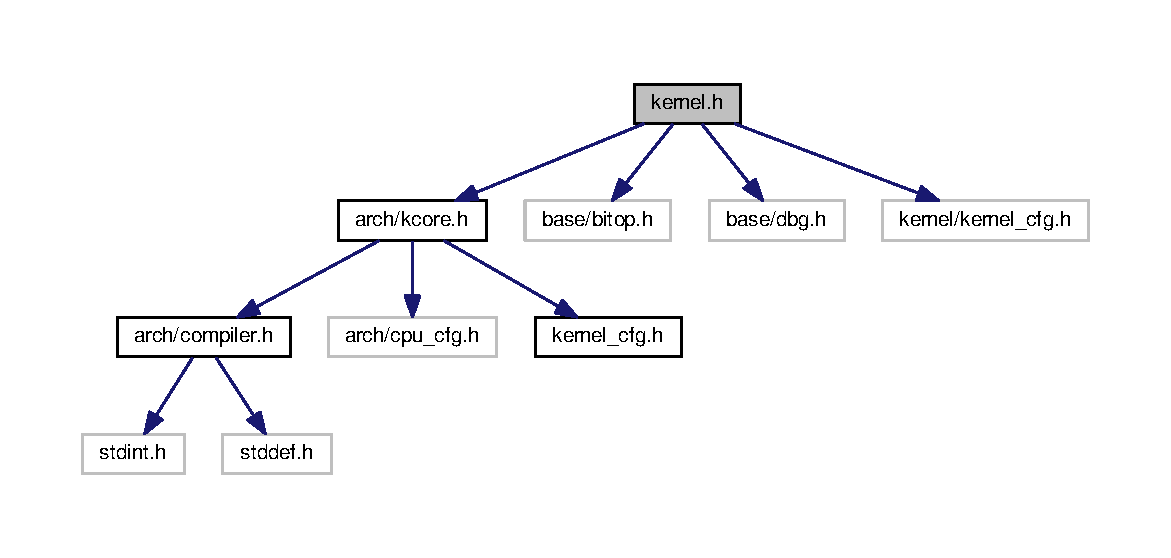
\includegraphics[width=350pt]{kernel_8h__incl}
\end{center}
\end{figure}
This graph shows which files directly or indirectly include this file\-:\nopagebreak
\begin{figure}[H]
\begin{center}
\leavevmode
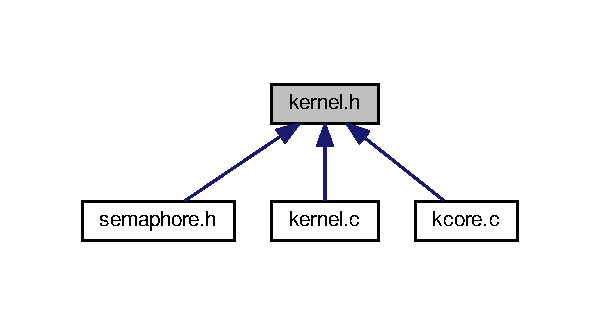
\includegraphics[width=288pt]{kernel_8h__dep__incl}
\end{center}
\end{figure}
\subsubsection*{Data Structures}
\begin{DoxyCompactItemize}
\item 
struct \hyperlink{structesThd}{es\-Thd}
\begin{DoxyCompactList}\small\item\em Thread structure. \end{DoxyCompactList}\item 
struct \hyperlink{structesThd_1_1thdL__}{es\-Thd\-::thd\-L\-\_\-}
\begin{DoxyCompactList}\small\item\em Thread linked List structure. \end{DoxyCompactList}\item 
struct \hyperlink{structesThdQ}{es\-Thd\-Q}
\begin{DoxyCompactList}\small\item\em Thread Queue structure. \end{DoxyCompactList}\item 
struct \hyperlink{structesThdQ_1_1pbm__}{es\-Thd\-Q\-::pbm\-\_\-}
\begin{DoxyCompactList}\small\item\em Priority Bit Map structure. \end{DoxyCompactList}\item 
struct \hyperlink{structesThdQ_1_1thdLSent__}{es\-Thd\-Q\-::thd\-L\-Sent\-\_\-}
\begin{DoxyCompactList}\small\item\em Thread linked list sentinel structure. \end{DoxyCompactList}\item 
struct \hyperlink{structesVTmr}{es\-V\-Tmr}
\begin{DoxyCompactList}\small\item\em Virtual Timer structure. \end{DoxyCompactList}\item 
struct \hyperlink{structesVTmr_1_1tmrL__}{es\-V\-Tmr\-::tmr\-L\-\_\-}
\begin{DoxyCompactList}\small\item\em Virtual Timer linked list structure. \end{DoxyCompactList}\item 
struct \hyperlink{structkernCtrl__}{kern\-Ctrl\-\_\-}
\begin{DoxyCompactList}\small\item\em Kernel control block structure. \end{DoxyCompactList}\end{DoxyCompactItemize}
\subsubsection*{Macros}
\begin{DoxyCompactItemize}
\item 
\#define \hyperlink{group__kern__id_ga06861cd0f6159ea9578193418c4eedf3}{E\-S\-\_\-\-K\-E\-R\-N\-\_\-\-V\-E\-R\-\_\-\-M\-A\-J\-O\-R}~1ul
\begin{DoxyCompactList}\small\item\em Identifies kernel major version number. \end{DoxyCompactList}\item 
\#define \hyperlink{group__kern__id_gaba74930b21c9c629a2589437f1e2584c}{E\-S\-\_\-\-K\-E\-R\-N\-\_\-\-V\-E\-R\-\_\-\-M\-I\-N\-O\-R}~0ul
\begin{DoxyCompactList}\small\item\em Identifies kernel minor version number. \end{DoxyCompactList}\item 
\#define \hyperlink{group__kern__id_gaa04466b958eeef9d02afadd6481abe5f}{E\-S\-\_\-\-K\-E\-R\-N\-\_\-\-V\-E\-R\-\_\-\-P\-A\-T\-C\-H}~0ul
\begin{DoxyCompactList}\small\item\em Identifies kernel patch level. \end{DoxyCompactList}\item 
\#define \hyperlink{group__kern__id_gacde22f7336a3c1c032dfc0ee3b94f506}{E\-S\-\_\-\-K\-E\-R\-N\-\_\-\-V\-E\-R}~(((\hyperlink{group__kern__id_ga06861cd0f6159ea9578193418c4eedf3}{E\-S\-\_\-\-K\-E\-R\-N\-\_\-\-V\-E\-R\-\_\-\-M\-A\-J\-O\-R}) $<$$<$ 24) $|$ (\hyperlink{group__kern__id_gaba74930b21c9c629a2589437f1e2584c}{E\-S\-\_\-\-K\-E\-R\-N\-\_\-\-V\-E\-R\-\_\-\-M\-I\-N\-O\-R} $<$$<$ 16) $|$ (\hyperlink{group__kern__id_gaa04466b958eeef9d02afadd6481abe5f}{E\-S\-\_\-\-K\-E\-R\-N\-\_\-\-V\-E\-R\-\_\-\-P\-A\-T\-C\-H}))
\begin{DoxyCompactList}\small\item\em Identifies the underlying kernel version number. \end{DoxyCompactList}\item 
\#define \hyperlink{group__kern__id_ga7a9484c6b09349e4eb82ba67c0989e25}{E\-S\-\_\-\-K\-E\-R\-N\-\_\-\-I\-D}~\char`\"{}e\-Solid -\/ R\-T Kernel\char`\"{}
\begin{DoxyCompactList}\small\item\em Kernel identification string. \end{DoxyCompactList}\item 
\#define \hyperlink{group__kern__thd_gaa707debebe3f98439911212b0cc8b3d1}{E\-S\-\_\-\-S\-T\-C\-K\-\_\-\-S\-I\-Z\-E}(elem)~\hyperlink{group__template__cpu__intf_gacb3a46e89d327fbaf5c122fe23877b24}{P\-O\-R\-T\-\_\-\-S\-T\-C\-K\-\_\-\-S\-I\-Z\-E}(elem)
\begin{DoxyCompactList}\small\item\em Converts the required stack elements into the stack array index. \end{DoxyCompactList}\item 
\#define \hyperlink{group__kern__thd_gaa9562c0ae61ad207e40486f952c5c7b3}{E\-S\-\_\-\-D\-E\-F\-\_\-\-T\-H\-D\-\_\-\-P\-R\-I\-O\-\_\-\-M\-A\-X}~(\hyperlink{group__template__kern__cfg_ga56bd89fe76f7fe22f3d8805bc3c68892}{C\-F\-G\-\_\-\-S\-C\-H\-E\-D\-\_\-\-P\-R\-I\-O\-\_\-\-L\-V\-L} -\/ 2u)
\begin{DoxyCompactList}\small\item\em Maximum level of priority possible for application thread. \end{DoxyCompactList}\item 
\#define \hyperlink{group__kern__thd_ga4dc54b2d44aa0656de70c7357733f4e4}{E\-S\-\_\-\-D\-E\-F\-\_\-\-T\-H\-D\-\_\-\-P\-R\-I\-O\-\_\-\-M\-I\-N}~(1u)
\begin{DoxyCompactList}\small\item\em Minimum level of priority possible for application thread. \end{DoxyCompactList}\end{DoxyCompactItemize}
\subsubsection*{Typedefs}
\begin{DoxyCompactItemize}
\item 
typedef struct \hyperlink{structesThd}{es\-Thd} \hyperlink{group__kern__thd_ga62e3a3ca0a4597a19c43cb8868810d82}{es\-Thd\-\_\-\-T}
\begin{DoxyCompactList}\small\item\em Thread type. \end{DoxyCompactList}\item 
typedef \hyperlink{group__template__cpu__intf_ga13cc91970e3e05fe4210440c068d3f4a}{port\-Stck\-\_\-\-T} \hyperlink{group__kern__thd_ga24160ddd0cb0327108cc652bfe6a49e5}{es\-Stck\-\_\-\-T}
\begin{DoxyCompactList}\small\item\em Stack type. \end{DoxyCompactList}\item 
typedef struct \hyperlink{structesThdQ}{es\-Thd\-Q} \hyperlink{group__kern__thdq_ga7a1a060699e83a01512ebb5540019556}{es\-Thd\-Q\-\_\-\-T}
\begin{DoxyCompactList}\small\item\em Thread queue type. \end{DoxyCompactList}\item 
typedef uint\-\_\-fast32\-\_\-t \hyperlink{group__kern__vtmr_ga844873888c186ee81eb66620dadb0451}{es\-Tick\-\_\-\-T}
\begin{DoxyCompactList}\small\item\em Timer tick type. \end{DoxyCompactList}\item 
typedef struct \hyperlink{structesVTmr}{es\-V\-Tmr} \hyperlink{group__kern__vtmr_ga3c020f0ca54ff412bc1d1505502d2afc}{es\-V\-Tmr\-\_\-\-T}
\begin{DoxyCompactList}\small\item\em Virtual Timer type. \end{DoxyCompactList}\item 
typedef enum \hyperlink{group__kern__ctrl_gac9be6bfeddbd6af148cdb3867fbc24af}{es\-Kern\-State} \hyperlink{group__kern__ctrl_gab5edef44fe53303f96dc5e9f567babaf}{es\-Kern\-State\-\_\-\-T}
\begin{DoxyCompactList}\small\item\em Kernel state type. \end{DoxyCompactList}\item 
typedef port\-Reg\-\_\-\-T \hyperlink{group__kern__lock_gad8b2b8257c3bf42c064adb66c0d45e2e}{es\-Lock\-Ctx\-\_\-\-T}
\begin{DoxyCompactList}\small\item\em Kernel lock context type. \end{DoxyCompactList}\end{DoxyCompactItemize}
\subsubsection*{Enumerations}
\begin{DoxyCompactItemize}
\item 
enum \hyperlink{group__kern__ctrl_gac9be6bfeddbd6af148cdb3867fbc24af}{es\-Kern\-State} \{ \\*
\hyperlink{group__kern__ctrl_ggac9be6bfeddbd6af148cdb3867fbc24afa31a7e1ee10bcd82aaf8f5eca06ecdbe8}{E\-S\-\_\-\-K\-E\-R\-N\-\_\-\-R\-U\-N} = 0x00u, 
\\*
\hyperlink{group__kern__ctrl_ggac9be6bfeddbd6af148cdb3867fbc24afa62e34103bea61ea0b7a9816180a43905}{E\-S\-\_\-\-K\-E\-R\-N\-\_\-\-I\-N\-T\-S\-R\-V\-\_\-\-R\-U\-N} = 0x01u, 
\\*
\hyperlink{group__kern__ctrl_ggac9be6bfeddbd6af148cdb3867fbc24afa4e5b5c809ea9cdbae536b701003278cc}{E\-S\-\_\-\-K\-E\-R\-N\-\_\-\-L\-O\-C\-K} = 0x02u, 
\\*
\hyperlink{group__kern__ctrl_ggac9be6bfeddbd6af148cdb3867fbc24afa2b35c503975df4c289e9cbff3e815f8b}{E\-S\-\_\-\-K\-E\-R\-N\-\_\-\-I\-N\-T\-S\-R\-V\-\_\-\-L\-O\-C\-K} = 0x03u, 
\\*
\hyperlink{group__kern__ctrl_ggac9be6bfeddbd6af148cdb3867fbc24afad45a94c8b4975fd162d683201a75cceb}{E\-S\-\_\-\-K\-E\-R\-N\-\_\-\-S\-L\-E\-E\-P} = 0x06u, 
\\*
\hyperlink{group__kern__ctrl_ggac9be6bfeddbd6af148cdb3867fbc24afacad35dc43528f96d27696db584f05cff}{E\-S\-\_\-\-K\-E\-R\-N\-\_\-\-I\-N\-I\-T} = 0x08u, 
\\*
\hyperlink{group__kern__ctrl_ggac9be6bfeddbd6af148cdb3867fbc24afa089165cac55f315953335f5ffe41b7c4}{E\-S\-\_\-\-K\-E\-R\-N\-\_\-\-I\-N\-A\-C\-T\-I\-V\-E} = 0x10u
 \}
\begin{DoxyCompactList}\small\item\em Kernel state enumeration. \end{DoxyCompactList}\end{DoxyCompactItemize}
\subsubsection*{Functions}
\begin{DoxyCompactItemize}
\item 
void \hyperlink{group__kern__general_ga9e9ff699d62d6035cd51121bb3140704}{es\-Kern\-Init} (void)
\begin{DoxyCompactList}\small\item\em Initialize kernel internal data structures. \end{DoxyCompactList}\item 
P\-O\-R\-T\-\_\-\-C\-\_\-\-N\-O\-R\-E\-T\-U\-R\-N void \hyperlink{group__kern__general_ga0e7a0a6b9c02df58de0f98de0229a09d}{es\-Kern\-Start} (void)
\begin{DoxyCompactList}\small\item\em Start the multi-\/threading. \end{DoxyCompactList}\item 
void \hyperlink{group__kern__general_ga3182e4c1a47897109d0a429b10a2483e}{es\-Kern\-Sys\-Tmr} (void)
\begin{DoxyCompactList}\small\item\em Process the system timer event. \end{DoxyCompactList}\item 
void \hyperlink{group__kern__general_gac0d578bcd4a10b2c8e5fc90f0b86ccec}{es\-Kern\-Isr\-Enter\-I} (void)
\begin{DoxyCompactList}\small\item\em Enter Interrupt Service Routine. \end{DoxyCompactList}\item 
void \hyperlink{group__kern__general_gaa6347925fff1684b5425dd2857c27129}{es\-Kern\-Isr\-Exit\-I} (void)
\begin{DoxyCompactList}\small\item\em Exit Interrupt Service Routine. \end{DoxyCompactList}\item 
void \hyperlink{group__kern__lock_gaa3ca4a02fafcfb840442506f42175a13}{es\-Kern\-Lock\-Int\-Enter} (\hyperlink{group__kern__lock_gad8b2b8257c3bf42c064adb66c0d45e2e}{es\-Lock\-Ctx\-\_\-\-T} $\ast$lock\-Ctx)
\begin{DoxyCompactList}\small\item\em Enter a critical code lock. \end{DoxyCompactList}\item 
void \hyperlink{group__kern__lock_gad8cb192a48802804cc12162edd18668d}{es\-Kern\-Lock\-Int\-Exit} (\hyperlink{group__kern__lock_gad8b2b8257c3bf42c064adb66c0d45e2e}{es\-Lock\-Ctx\-\_\-\-T} lock\-Ctx)
\begin{DoxyCompactList}\small\item\em Exit a critical code lock. \end{DoxyCompactList}\item 
void \hyperlink{group__kern__lock_ga6dd45355c20a10f7272bd39670353428}{es\-Kern\-Lock\-Enter\-I} (void)
\begin{DoxyCompactList}\small\item\em Lock the scheduler. \end{DoxyCompactList}\item 
void \hyperlink{group__kern__lock_ga3287aefb2c7dd24672c716d86a008ad3}{es\-Kern\-Lock\-Exit\-I} (void)
\begin{DoxyCompactList}\small\item\em Unlock the scheduler. \end{DoxyCompactList}\item 
void \hyperlink{group__kern__lock_ga86ec4f4cbaa889b0f23c7e2ebdcbbb97}{es\-Kern\-Lock\-Enter} (void)
\begin{DoxyCompactList}\small\item\em Lock the scheduler. \end{DoxyCompactList}\item 
void \hyperlink{group__kern__lock_gaf1eec663f7cc5c414b113901382ccd82}{es\-Kern\-Lock\-Exit} (void)
\begin{DoxyCompactList}\small\item\em Unlock the scheduler. \end{DoxyCompactList}\item 
void \hyperlink{group__kern__thd_gac91734f3ee867b519f59bf81cc7fde88}{es\-Thd\-Init} (\hyperlink{group__kern__thd_ga62e3a3ca0a4597a19c43cb8868810d82}{es\-Thd\-\_\-\-T} $\ast$thd, void($\ast$fn)(void $\ast$), void $\ast$arg, \hyperlink{group__template__cpu__intf_ga13cc91970e3e05fe4210440c068d3f4a}{port\-Stck\-\_\-\-T} $\ast$stck, size\-\_\-t stck\-Size, uint8\-\_\-t prio)
\begin{DoxyCompactList}\small\item\em Initialize the specified thread. \end{DoxyCompactList}\item 
void \hyperlink{group__kern__thd_gac9d1eac76f26096614e8196bcfd8b905}{es\-Thd\-Term} (\hyperlink{group__kern__thd_ga62e3a3ca0a4597a19c43cb8868810d82}{es\-Thd\-\_\-\-T} $\ast$thd)
\begin{DoxyCompactList}\small\item\em Terminate the specified thread. \end{DoxyCompactList}\item 
static \hyperlink{group__template__compiler_ga87952d6e574c7f437503926e833ba345}{P\-O\-R\-T\-\_\-\-C\-\_\-\-I\-N\-L\-I\-N\-E} \hyperlink{group__kern__thd_ga62e3a3ca0a4597a19c43cb8868810d82}{es\-Thd\-\_\-\-T} $\ast$ \hyperlink{group__kern__thd_gae2a2c5fe0128d446a64512b0714bfb6d}{es\-Thd\-Get\-Id} (void)
\begin{DoxyCompactList}\small\item\em Get the current thread I\-D. \end{DoxyCompactList}\item 
static \hyperlink{group__template__compiler_ga87952d6e574c7f437503926e833ba345}{P\-O\-R\-T\-\_\-\-C\-\_\-\-I\-N\-L\-I\-N\-E} uint8\-\_\-t \hyperlink{group__kern__thd_ga6d2d033dc7e1226eccf4a51c666678ad}{es\-Thd\-Get\-Prio} (\hyperlink{group__kern__thd_ga62e3a3ca0a4597a19c43cb8868810d82}{es\-Thd\-\_\-\-T} $\ast$thd)
\begin{DoxyCompactList}\small\item\em Get the priority of a thread. \end{DoxyCompactList}\item 
void \hyperlink{group__kern__thd_ga8eaa731d0026a8a1667d4422d5031df6}{es\-Thd\-Set\-Prio\-I} (\hyperlink{group__kern__thd_ga62e3a3ca0a4597a19c43cb8868810d82}{es\-Thd\-\_\-\-T} $\ast$thd, uint8\-\_\-t prio)
\begin{DoxyCompactList}\small\item\em Set the priority of a thread. \end{DoxyCompactList}\item 
void \hyperlink{group__kern__thdq_gaddd5fe0557c91559b9452beb0fc236fd}{es\-Thd\-Q\-Init} (\hyperlink{group__kern__thdq_ga7a1a060699e83a01512ebb5540019556}{es\-Thd\-Q\-\_\-\-T} $\ast$thd\-Q)
\begin{DoxyCompactList}\small\item\em Initialize Thread Queue. \end{DoxyCompactList}\item 
void \hyperlink{group__kern__thdq_gaa5f19b32a7f0c42616b5270dcbd73a3e}{es\-Thd\-Q\-Term} (\hyperlink{group__kern__thdq_ga7a1a060699e83a01512ebb5540019556}{es\-Thd\-Q\-\_\-\-T} $\ast$thd\-Q)
\begin{DoxyCompactList}\small\item\em Terminate Thread Queue. \end{DoxyCompactList}\item 
void \hyperlink{group__kern__thdq_ga9da1e71c137d8adb8c9bdead7052b5fa}{es\-Thd\-Q\-Add\-I} (\hyperlink{group__kern__thdq_ga7a1a060699e83a01512ebb5540019556}{es\-Thd\-Q\-\_\-\-T} $\ast$thd\-Q, \hyperlink{group__kern__thd_ga62e3a3ca0a4597a19c43cb8868810d82}{es\-Thd\-\_\-\-T} $\ast$thd)
\begin{DoxyCompactList}\small\item\em Add a thread to the Thread Queue. \end{DoxyCompactList}\item 
void \hyperlink{group__kern__thdq_gaa18afa95e34035da03c5cb7ea3a96320}{es\-Thd\-Q\-Rm\-I} (\hyperlink{group__kern__thdq_ga7a1a060699e83a01512ebb5540019556}{es\-Thd\-Q\-\_\-\-T} $\ast$thd\-Q, \hyperlink{group__kern__thd_ga62e3a3ca0a4597a19c43cb8868810d82}{es\-Thd\-\_\-\-T} $\ast$thd)
\begin{DoxyCompactList}\small\item\em Removes the thread from the Thread Queue. \end{DoxyCompactList}\item 
\hyperlink{group__kern__thd_ga62e3a3ca0a4597a19c43cb8868810d82}{es\-Thd\-\_\-\-T} $\ast$ \hyperlink{group__kern__thdq_ga1670c123f31c346b24ec9d2b7ae35f88}{es\-Thd\-Q\-Fetch\-I} (const \hyperlink{group__kern__thdq_ga7a1a060699e83a01512ebb5540019556}{es\-Thd\-Q\-\_\-\-T} $\ast$thd\-Q)
\begin{DoxyCompactList}\small\item\em Fetch the first high priority thread from the Thread Queue. \end{DoxyCompactList}\item 
\hyperlink{group__kern__thd_ga62e3a3ca0a4597a19c43cb8868810d82}{es\-Thd\-\_\-\-T} $\ast$ \hyperlink{group__kern__thdq_gae365b14292f1496a90d876baec84fb4e}{es\-Thd\-Q\-Fetch\-Rotate\-I} (\hyperlink{group__kern__thdq_ga7a1a060699e83a01512ebb5540019556}{es\-Thd\-Q\-\_\-\-T} $\ast$thd\-Q, uint\-\_\-fast8\-\_\-t prio)
\begin{DoxyCompactList}\small\item\em Fetch the next thread and rotate thread linked list. \end{DoxyCompactList}\item 
\hyperlink{group__template__compiler_ga74fbee312f9185efb602f89d21b53404}{bool\-\_\-\-T} \hyperlink{group__kern__thdq_gacf2687b82ce64e2154d97fd3b69a4ab5}{es\-Thd\-Q\-Is\-Empty} (const \hyperlink{group__kern__thdq_ga7a1a060699e83a01512ebb5540019556}{es\-Thd\-Q\-\_\-\-T} $\ast$thd\-Q)
\begin{DoxyCompactList}\small\item\em Is thread queue empty. \end{DoxyCompactList}\item 
void \hyperlink{group__kern__sched_ga73e14b1860ce824c822adc407aee0977}{es\-Sched\-Rdy\-Add\-I} (\hyperlink{group__kern__thd_ga62e3a3ca0a4597a19c43cb8868810d82}{es\-Thd\-\_\-\-T} $\ast$thd)
\begin{DoxyCompactList}\small\item\em Add thread {\ttfamily thd} to the ready thread list and notify the scheduler. \end{DoxyCompactList}\item 
void \hyperlink{group__kern__sched_ga0b8263c5024ebb59cd9b95cc9253b44d}{es\-Sched\-Rdy\-Rm\-I} (\hyperlink{group__kern__thd_ga62e3a3ca0a4597a19c43cb8868810d82}{es\-Thd\-\_\-\-T} $\ast$thd)
\begin{DoxyCompactList}\small\item\em Remove thread {\ttfamily thd} from the ready thread list and notify the scheduler. \end{DoxyCompactList}\item 
void \hyperlink{group__kern__sched_gaf90e487bfce974dafaeed5009e189810}{es\-Sched\-Yield\-I} (void)
\begin{DoxyCompactList}\small\item\em Force the scheduler invocation which will evaluate all ready threads and switch to ready thread with the highest priority. \end{DoxyCompactList}\item 
void \hyperlink{group__kern__sched_gafbea29b376b29f11bbfc48a0f5144e9a}{es\-Sched\-Yield\-Isr\-I} (void)
\begin{DoxyCompactList}\small\item\em Force the scheduler invocation which will evaluate all ready threads and switch to ready thread with the highest priority. \end{DoxyCompactList}\item 
void \hyperlink{group__kern__vtmr_ga45fe650eac73e7fe203cc81565401555}{es\-V\-Tmr\-Init\-I} (\hyperlink{group__kern__vtmr_ga3c020f0ca54ff412bc1d1505502d2afc}{es\-V\-Tmr\-\_\-\-T} $\ast$v\-Tmr, \hyperlink{group__kern__vtmr_ga844873888c186ee81eb66620dadb0451}{es\-Tick\-\_\-\-T} tick, void($\ast$fn)(void $\ast$), void $\ast$arg)
\begin{DoxyCompactList}\small\item\em Add and start a new virtual timer. \end{DoxyCompactList}\item 
void \hyperlink{group__kern__vtmr_gad932cf00aec4ba03a0df02ccc493c4c2}{es\-V\-Tmr\-Init} (\hyperlink{group__kern__vtmr_ga3c020f0ca54ff412bc1d1505502d2afc}{es\-V\-Tmr\-\_\-\-T} $\ast$v\-Tmr, \hyperlink{group__kern__vtmr_ga844873888c186ee81eb66620dadb0451}{es\-Tick\-\_\-\-T} tick, void($\ast$fn)(void $\ast$), void $\ast$arg)
\begin{DoxyCompactList}\small\item\em Add and start a new virtual timer. \end{DoxyCompactList}\item 
void \hyperlink{group__kern__vtmr_ga96bb2c81f649c0305dfd08d1c79b2e37}{es\-V\-Tmr\-Term\-I} (\hyperlink{group__kern__vtmr_ga3c020f0ca54ff412bc1d1505502d2afc}{es\-V\-Tmr\-\_\-\-T} $\ast$v\-Tmr)
\begin{DoxyCompactList}\small\item\em Cancel and remove a virtual timer. \end{DoxyCompactList}\item 
void \hyperlink{group__kern__vtmr_gad6ec93a68e3526f18ed926cd441878cd}{es\-V\-Tmr\-Term} (\hyperlink{group__kern__vtmr_ga3c020f0ca54ff412bc1d1505502d2afc}{es\-V\-Tmr\-\_\-\-T} $\ast$v\-Tmr)
\begin{DoxyCompactList}\small\item\em Cancel and remove a virtual timer. \end{DoxyCompactList}\item 
void \hyperlink{group__kern__vtmr_ga26d10c6aaa0cd1d04261d2c9911e890d}{es\-V\-Tmr\-Delay} (\hyperlink{group__kern__vtmr_ga844873888c186ee81eb66620dadb0451}{es\-Tick\-\_\-\-T} tick)
\begin{DoxyCompactList}\small\item\em Delay for specified amount of ticks. \end{DoxyCompactList}\item 
\hyperlink{group__kern__vtmr_ga844873888c186ee81eb66620dadb0451}{es\-Tick\-\_\-\-T} \hyperlink{group__kern__time_gacb0d88d6a7e467dc37a6a9a85945aaa6}{es\-Sys\-Tmr\-Tick\-Get} (void)
\begin{DoxyCompactList}\small\item\em Get the current tick value. \end{DoxyCompactList}\item 
void \hyperlink{group__kern__hook_ga9a0d562969acef0121136b11be7b4728}{user\-Pre\-Sys\-Tmr} (void)
\begin{DoxyCompactList}\small\item\em System timer hook function, called from system system timer I\-S\-R function before the kernel functions. \end{DoxyCompactList}\item 
void \hyperlink{group__kern__hook_gaac77966856c9a299cda4794cbcc87edf}{user\-Pre\-Kern\-Init} (void)
\begin{DoxyCompactList}\small\item\em Kernel initialization hook function, called from \hyperlink{group__kern__general_ga9e9ff699d62d6035cd51121bb3140704}{es\-Kern\-Init()} function before kernel initialization. \end{DoxyCompactList}\item 
void \hyperlink{group__kern__hook_ga3579ac6964a314ad03d13da0507f57e8}{user\-Post\-Kern\-Init} (void)
\begin{DoxyCompactList}\small\item\em Kernel initialization hook function, called from \hyperlink{group__kern__general_ga9e9ff699d62d6035cd51121bb3140704}{es\-Kern\-Init()} function after kernel initialization. \end{DoxyCompactList}\item 
void \hyperlink{group__kern__hook_gaac505ab4c72e0fb346ca441d6def327d}{user\-Pre\-Kern\-Start} (void)
\begin{DoxyCompactList}\small\item\em Kernel start hook function, called from \hyperlink{group__kern__general_ga0e7a0a6b9c02df58de0f98de0229a09d}{es\-Kern\-Start()} function. \end{DoxyCompactList}\item 
void \hyperlink{group__kern__hook_ga64ca864d0ff2aaa532208d7c2b88bdb3}{user\-Post\-Thd\-Init} (\hyperlink{group__kern__thd_ga62e3a3ca0a4597a19c43cb8868810d82}{es\-Thd\-\_\-\-T} $\ast$thd)
\begin{DoxyCompactList}\small\item\em Thread initialization end hook function, called from \hyperlink{group__kern__thd_gac91734f3ee867b519f59bf81cc7fde88}{es\-Thd\-Init()} function. \end{DoxyCompactList}\item 
void \hyperlink{group__kern__hook_ga076ad76633999c9d5e245e3b5c6e0c09}{user\-Pre\-Thd\-Term} (void)
\begin{DoxyCompactList}\small\item\em Thread terminate hook function, called from \hyperlink{group__kern__thd_gac9d1eac76f26096614e8196bcfd8b905}{es\-Thd\-Term()} or when a thread terminates itself. \end{DoxyCompactList}\item 
void \hyperlink{group__kern__hook_ga2bd40d82f768787c3dab2f4df336685e}{user\-Pre\-Idle} (void)
\begin{DoxyCompactList}\small\item\em Pre Idle hook function, called from idle thread, just before entering idle period. \end{DoxyCompactList}\item 
void \hyperlink{group__kern__hook_ga7ca4a96cbe5064d633298d1d172fd4e7}{user\-Post\-Idle} (void)
\begin{DoxyCompactList}\small\item\em Post idle hook function, called from idle thread, just after exiting idle period. \end{DoxyCompactList}\item 
void \hyperlink{group__kern__hook_ga74a38c965110d0f2f2e44e13571fe3fc}{user\-Pre\-Ctx\-Sw} (\hyperlink{group__kern__thd_ga62e3a3ca0a4597a19c43cb8868810d82}{es\-Thd\-\_\-\-T} $\ast$old\-Thd, \hyperlink{group__kern__thd_ga62e3a3ca0a4597a19c43cb8868810d82}{es\-Thd\-\_\-\-T} $\ast$new\-Thd)
\begin{DoxyCompactList}\small\item\em Kernel context switch hook function, called from \hyperlink{group__kern__sched_gaf90e487bfce974dafaeed5009e189810}{es\-Sched\-Yield\-I()} and \hyperlink{group__kern__sched_gafbea29b376b29f11bbfc48a0f5144e9a}{es\-Sched\-Yield\-Isr\-I()} functions just before context switch. \end{DoxyCompactList}\end{DoxyCompactItemize}
\subsubsection*{Variables}
\begin{DoxyCompactItemize}
\item 
const struct \hyperlink{structkernCtrl__}{kern\-Ctrl\-\_\-} \hyperlink{group__kern__ctrl_ga93a7ee7768ffd94201bf1795a543194b}{Kern\-Ctrl}
\begin{DoxyCompactList}\small\item\em Kernel control block. \end{DoxyCompactList}\end{DoxyCompactItemize}


\subsubsection{Detailed Description}
Main kernel interface. \begin{DoxyAuthor}{Author}
Nenad Radulovic 
\end{DoxyAuthor}

\hypertarget{kernel__cfg_8h}{\subsection{kernel\-\_\-cfg.\-h File Reference}
\label{kernel__cfg_8h}\index{kernel\-\_\-cfg.\-h@{kernel\-\_\-cfg.\-h}}
}


Configuration of Kernel -\/ Template.  


This graph shows which files directly or indirectly include this file\-:\nopagebreak
\begin{figure}[H]
\begin{center}
\leavevmode
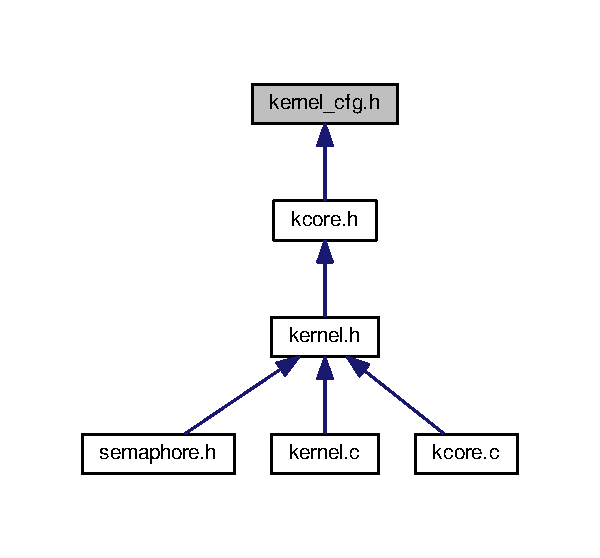
\includegraphics[width=288pt]{kernel__cfg_8h__dep__incl}
\end{center}
\end{figure}
\subsubsection*{Macros}
\begin{Indent}{\bf Kernel configuration options and settings}\par
{\em Kernel default configuration }\begin{DoxyCompactItemize}
\item 
\#define \hyperlink{group__template__kern__cfg_ga56bd89fe76f7fe22f3d8805bc3c68892}{C\-F\-G\-\_\-\-S\-C\-H\-E\-D\-\_\-\-P\-R\-I\-O\-\_\-\-L\-V\-L}~8\-U
\begin{DoxyCompactList}\small\item\em Scheduler priority levels. \end{DoxyCompactList}\item 
\#define \hyperlink{group__template__kern__cfg_ga0bd286f16bb67585f14c4d1e45be8ad1}{C\-F\-G\-\_\-\-S\-C\-H\-E\-D\-\_\-\-T\-I\-M\-E\-\_\-\-Q\-U\-A\-N\-T\-U\-M}~10\-U
\begin{DoxyCompactList}\small\item\em Scheduler Round-\/\-Robin time quantum. \end{DoxyCompactList}\item 
\#define \hyperlink{group__template__kern__cfg_ga4e6ab4994b34501bb71e75717b093376}{C\-F\-G\-\_\-\-S\-C\-H\-E\-D\-\_\-\-P\-O\-W\-E\-R\-\_\-\-S\-A\-V\-E}~0\-U
\begin{DoxyCompactList}\small\item\em Enable/disable scheduler power savings mode. \end{DoxyCompactList}\item 
\#define \hyperlink{group__template__kern__cfg_ga5f07eea2a4be92cf0358f52eba6800c9}{C\-F\-G\-\_\-\-S\-Y\-S\-T\-M\-R\-\_\-\-A\-D\-A\-P\-T\-I\-V\-E\-\_\-\-M\-O\-D\-E}~0\-U
\begin{DoxyCompactList}\small\item\em System timer mode. \end{DoxyCompactList}\item 
\#define \hyperlink{group__template__kern__cfg_ga4e46164ae5a37bfc54c67b6f01d93eb1}{C\-F\-G\-\_\-\-S\-Y\-S\-T\-M\-R\-\_\-\-E\-V\-E\-N\-T\-\_\-\-F\-R\-E\-Q\-U\-E\-N\-C\-Y}~100\-U\-L
\begin{DoxyCompactList}\small\item\em The frequency of system tick event. \end{DoxyCompactList}\item 
\#define \hyperlink{group__template__kern__cfg_gad69eef523459c5ab485ce2f62bddceca}{C\-F\-G\-\_\-\-S\-Y\-S\-T\-M\-R\-\_\-\-T\-I\-C\-K\-\_\-\-T\-Y\-P\-E}~2\-U
\begin{DoxyCompactList}\small\item\em The size of the system timer counter. \end{DoxyCompactList}\end{DoxyCompactItemize}
\end{Indent}
\begin{Indent}{\bf Kernel hooks}\par
\begin{DoxyCompactItemize}
\item 
\#define \hyperlink{group__template__kern__cfg_gaa130bc9f72010b44b4b06618d8f8d0bc}{C\-F\-G\-\_\-\-H\-O\-O\-K\-\_\-\-P\-R\-E\-\_\-\-S\-Y\-S\-T\-M\-R\-\_\-\-E\-V\-E\-N\-T}~0\-U
\begin{DoxyCompactList}\small\item\em System timer event hook function. \end{DoxyCompactList}\item 
\#define \hyperlink{group__template__kern__cfg_ga4093113f2105d2716f86c6509a6e643a}{C\-F\-G\-\_\-\-H\-O\-O\-K\-\_\-\-P\-R\-E\-\_\-\-K\-E\-R\-N\-\_\-\-I\-N\-I\-T}~0\-U
\begin{DoxyCompactList}\small\item\em Pre kernel initialization hook function. \end{DoxyCompactList}\item 
\#define \hyperlink{group__template__kern__cfg_ga85dea823714335c2ec9e9f7750996e83}{C\-F\-G\-\_\-\-H\-O\-O\-K\-\_\-\-P\-O\-S\-T\-\_\-\-K\-E\-R\-N\-\_\-\-I\-N\-I\-T}~0\-U
\begin{DoxyCompactList}\small\item\em Post kernel initialization hook function. \end{DoxyCompactList}\item 
\#define \hyperlink{group__template__kern__cfg_gad67d998118375811b0f3e63543311661}{C\-F\-G\-\_\-\-H\-O\-O\-K\-\_\-\-P\-R\-E\-\_\-\-K\-E\-R\-N\-\_\-\-S\-T\-A\-R\-T}~0\-U
\begin{DoxyCompactList}\small\item\em Pre kernel start hook function. \end{DoxyCompactList}\item 
\#define \hyperlink{group__template__kern__cfg_ga23deae306171d1a8dda4d0e33efdb6bb}{C\-F\-G\-\_\-\-H\-O\-O\-K\-\_\-\-P\-O\-S\-T\-\_\-\-T\-H\-D\-\_\-\-I\-N\-I\-T}~0\-U
\begin{DoxyCompactList}\small\item\em Post thread initialization hook function. \end{DoxyCompactList}\item 
\#define \hyperlink{group__template__kern__cfg_ga9c7dd4e009a89e9cffb0f9b404bc6250}{C\-F\-G\-\_\-\-H\-O\-O\-K\-\_\-\-P\-R\-E\-\_\-\-T\-H\-D\-\_\-\-T\-E\-R\-M}~0\-U
\begin{DoxyCompactList}\small\item\em Pre thread termination hook function. \end{DoxyCompactList}\item 
\#define \hyperlink{group__template__kern__cfg_ga7c2b0410404256c4804758090401f7e4}{C\-F\-G\-\_\-\-H\-O\-O\-K\-\_\-\-P\-R\-E\-\_\-\-I\-D\-L\-E}~0\-U
\begin{DoxyCompactList}\small\item\em Pre idle hook function. \end{DoxyCompactList}\item 
\#define \hyperlink{group__template__kern__cfg_ga8f8751efe94964bef25673deca6b9b26}{C\-F\-G\-\_\-\-H\-O\-O\-K\-\_\-\-P\-O\-S\-T\-\_\-\-I\-D\-L\-E}~0\-U
\begin{DoxyCompactList}\small\item\em Post idle hook function. \end{DoxyCompactList}\item 
\#define \hyperlink{group__template__kern__cfg_gac84acbf84222018398089920dd429635}{C\-F\-G\-\_\-\-H\-O\-O\-K\-\_\-\-P\-R\-E\-\_\-\-C\-T\-X\-\_\-\-S\-W}~0\-U
\begin{DoxyCompactList}\small\item\em Pre context switch hook function. \end{DoxyCompactList}\end{DoxyCompactItemize}
\end{Indent}


\subsubsection{Detailed Description}
Configuration of Kernel -\/ Template. \begin{DoxyAuthor}{Author}
Nenad Radulovic 
\end{DoxyAuthor}

\hypertarget{profile_8h}{\subsection{profile.\-h File Reference}
\label{profile_8h}\index{profile.\-h@{profile.\-h}}
}


Family port specific configuration options.  


\subsubsection*{Macros}
\begin{Indent}{\bf Generic family defaults}\par
\begin{DoxyCompactItemize}
\item 
\#define \hyperlink{group__template__family__cfg_gaed6437f330e7be6f8d5a04a19cbe8776}{C\-P\-U\-\_\-\-D\-E\-F\-\_\-\-S\-Y\-S\-T\-M\-R\-\_\-\-M\-A\-X\-\_\-\-V\-A\-L}~0xfful
\begin{DoxyCompactList}\small\item\em System timer maximum value. \end{DoxyCompactList}\end{DoxyCompactItemize}
\end{Indent}


\subsubsection{Detailed Description}
Family port specific configuration options. \begin{DoxyAuthor}{Author}
Nenad Radulovic 
\end{DoxyAuthor}

\hypertarget{semaphore_8h}{\subsection{semaphore.\-h File Reference}
\label{semaphore_8h}\index{semaphore.\-h@{semaphore.\-h}}
}


Interface of semaphore.  


{\ttfamily \#include \char`\"{}kernel/kernel.\-h\char`\"{}}\\*
Include dependency graph for semaphore.\-h\-:\nopagebreak
\begin{figure}[H]
\begin{center}
\leavevmode
\includegraphics[width=350pt]{semaphore_8h__incl}
\end{center}
\end{figure}
\subsubsection*{Functions}
\begin{Indent}{\bf Function group}\par
{\em brief description }\begin{DoxyCompactItemize}
\item 
void \hyperlink{group__sem__intf_gae4481945af3c671b99e87b151de98085}{es\-Sem\-Init} (es\-Sem\-\_\-\-T $\ast$sem, es\-Sem\-Cnt\-\_\-\-T cnt)
\begin{DoxyCompactList}\small\item\em Initialize a semaphore. \end{DoxyCompactList}\item 
\hypertarget{group__sem__intf_ga897ad9e48bcf3fea3fa68897cbcf33d9}{void {\bfseries es\-Sem\-Term} (es\-Sem\-\_\-\-T $\ast$sem)}\label{group__sem__intf_ga897ad9e48bcf3fea3fa68897cbcf33d9}

\item 
void \hyperlink{group__sem__intf_gaf742af1a3888b602a45e4cd394f28550}{es\-Sem\-Wait} (es\-Sem\-\_\-\-T $\ast$sem)
\begin{DoxyCompactList}\small\item\em Wait on a semaphore. \end{DoxyCompactList}\item 
void \hyperlink{group__sem__intf_ga4f11d79edca489a754f9385ca7c89b36}{es\-Sem\-Wait\-Timeout} (es\-Sem\-\_\-\-T $\ast$sem, \hyperlink{group__kern__vtmr_ga844873888c186ee81eb66620dadb0451}{es\-Tick\-\_\-\-T} time)
\begin{DoxyCompactList}\small\item\em Wait on a semaphore. \end{DoxyCompactList}\item 
void \hyperlink{group__sem__intf_ga372df852afd413b4fe2e65591da2fe79}{es\-Sem\-Post} (es\-Sem\-\_\-\-T $\ast$sem)
\begin{DoxyCompactList}\small\item\em Increment the value of a semaphore. \end{DoxyCompactList}\end{DoxyCompactItemize}
\end{Indent}
\subsubsection*{Data types group}
\label{_amgrpca30459c90d6b7a12b3df0a1317e654e}%
brief description \begin{DoxyCompactItemize}
\item 
\hypertarget{group__sem__intf_gaf38e40d531c3eb3d03ab29c0a116b235}{\#define {\bfseries C\-F\-G\-\_\-\-S\-E\-M\-A\-P\-H\-O\-R\-E\-\_\-\-C\-N\-T\-\_\-\-T}~int16\-\_\-t}\label{group__sem__intf_gaf38e40d531c3eb3d03ab29c0a116b235}

\item 
\hypertarget{group__sem__intf_gaa080a10f59ad14ffb1e27d577b10e870}{typedef C\-F\-G\-\_\-\-S\-E\-M\-A\-P\-H\-O\-R\-E\-\_\-\-C\-N\-T\-\_\-\-T {\bfseries es\-Sem\-Cnt\-\_\-\-T}}\label{group__sem__intf_gaa080a10f59ad14ffb1e27d577b10e870}

\item 
\hypertarget{group__sem__intf_ga076de09738f0febcd417f15a9ac15a7e}{typedef struct es\-Sem {\bfseries es\-Sem\-\_\-\-T}}\label{group__sem__intf_ga076de09738f0febcd417f15a9ac15a7e}

\end{DoxyCompactItemize}


\subsubsection{Detailed Description}
Interface of semaphore. \begin{DoxyAuthor}{Author}
Nenad Radulovic
\end{DoxyAuthor}
Detailed description 
\hypertarget{sync_8dox}{\subsection{sync.\-dox File Reference}
\label{sync_8dox}\index{sync.\-dox@{sync.\-dox}}
}

\hypertarget{template_8dox}{\subsection{template.\-dox File Reference}
\label{template_8dox}\index{template.\-dox@{template.\-dox}}
}

%--- End generated contents ---

% Index
\newpage
\phantomsection
\addcontentsline{toc}{part}{Index}
\printindex

\end{document}
